% Options for packages loaded elsewhere
\PassOptionsToPackage{unicode}{hyperref}
\PassOptionsToPackage{hyphens}{url}
%
\documentclass[
]{article}
\usepackage{amsmath,amssymb}
\usepackage{lmodern}
\usepackage{iftex}
\ifPDFTeX
  \usepackage[T1]{fontenc}
  \usepackage[utf8]{inputenc}
  \usepackage{textcomp} % provide euro and other symbols
\else % if luatex or xetex
  \usepackage{unicode-math}
  \defaultfontfeatures{Scale=MatchLowercase}
  \defaultfontfeatures[\rmfamily]{Ligatures=TeX,Scale=1}
\fi
% Use upquote if available, for straight quotes in verbatim environments
\IfFileExists{upquote.sty}{\usepackage{upquote}}{}
\IfFileExists{microtype.sty}{% use microtype if available
  \usepackage[]{microtype}
  \UseMicrotypeSet[protrusion]{basicmath} % disable protrusion for tt fonts
}{}
\makeatletter
\@ifundefined{KOMAClassName}{% if non-KOMA class
  \IfFileExists{parskip.sty}{%
    \usepackage{parskip}
  }{% else
    \setlength{\parindent}{0pt}
    \setlength{\parskip}{6pt plus 2pt minus 1pt}}
}{% if KOMA class
  \KOMAoptions{parskip=half}}
\makeatother
\usepackage{xcolor}
\usepackage[margin=1in]{geometry}
\usepackage{color}
\usepackage{fancyvrb}
\newcommand{\VerbBar}{|}
\newcommand{\VERB}{\Verb[commandchars=\\\{\}]}
\DefineVerbatimEnvironment{Highlighting}{Verbatim}{commandchars=\\\{\}}
% Add ',fontsize=\small' for more characters per line
\usepackage{framed}
\definecolor{shadecolor}{RGB}{248,248,248}
\newenvironment{Shaded}{\begin{snugshade}}{\end{snugshade}}
\newcommand{\AlertTok}[1]{\textcolor[rgb]{0.94,0.16,0.16}{#1}}
\newcommand{\AnnotationTok}[1]{\textcolor[rgb]{0.56,0.35,0.01}{\textbf{\textit{#1}}}}
\newcommand{\AttributeTok}[1]{\textcolor[rgb]{0.77,0.63,0.00}{#1}}
\newcommand{\BaseNTok}[1]{\textcolor[rgb]{0.00,0.00,0.81}{#1}}
\newcommand{\BuiltInTok}[1]{#1}
\newcommand{\CharTok}[1]{\textcolor[rgb]{0.31,0.60,0.02}{#1}}
\newcommand{\CommentTok}[1]{\textcolor[rgb]{0.56,0.35,0.01}{\textit{#1}}}
\newcommand{\CommentVarTok}[1]{\textcolor[rgb]{0.56,0.35,0.01}{\textbf{\textit{#1}}}}
\newcommand{\ConstantTok}[1]{\textcolor[rgb]{0.00,0.00,0.00}{#1}}
\newcommand{\ControlFlowTok}[1]{\textcolor[rgb]{0.13,0.29,0.53}{\textbf{#1}}}
\newcommand{\DataTypeTok}[1]{\textcolor[rgb]{0.13,0.29,0.53}{#1}}
\newcommand{\DecValTok}[1]{\textcolor[rgb]{0.00,0.00,0.81}{#1}}
\newcommand{\DocumentationTok}[1]{\textcolor[rgb]{0.56,0.35,0.01}{\textbf{\textit{#1}}}}
\newcommand{\ErrorTok}[1]{\textcolor[rgb]{0.64,0.00,0.00}{\textbf{#1}}}
\newcommand{\ExtensionTok}[1]{#1}
\newcommand{\FloatTok}[1]{\textcolor[rgb]{0.00,0.00,0.81}{#1}}
\newcommand{\FunctionTok}[1]{\textcolor[rgb]{0.00,0.00,0.00}{#1}}
\newcommand{\ImportTok}[1]{#1}
\newcommand{\InformationTok}[1]{\textcolor[rgb]{0.56,0.35,0.01}{\textbf{\textit{#1}}}}
\newcommand{\KeywordTok}[1]{\textcolor[rgb]{0.13,0.29,0.53}{\textbf{#1}}}
\newcommand{\NormalTok}[1]{#1}
\newcommand{\OperatorTok}[1]{\textcolor[rgb]{0.81,0.36,0.00}{\textbf{#1}}}
\newcommand{\OtherTok}[1]{\textcolor[rgb]{0.56,0.35,0.01}{#1}}
\newcommand{\PreprocessorTok}[1]{\textcolor[rgb]{0.56,0.35,0.01}{\textit{#1}}}
\newcommand{\RegionMarkerTok}[1]{#1}
\newcommand{\SpecialCharTok}[1]{\textcolor[rgb]{0.00,0.00,0.00}{#1}}
\newcommand{\SpecialStringTok}[1]{\textcolor[rgb]{0.31,0.60,0.02}{#1}}
\newcommand{\StringTok}[1]{\textcolor[rgb]{0.31,0.60,0.02}{#1}}
\newcommand{\VariableTok}[1]{\textcolor[rgb]{0.00,0.00,0.00}{#1}}
\newcommand{\VerbatimStringTok}[1]{\textcolor[rgb]{0.31,0.60,0.02}{#1}}
\newcommand{\WarningTok}[1]{\textcolor[rgb]{0.56,0.35,0.01}{\textbf{\textit{#1}}}}
\usepackage{graphicx}
\makeatletter
\def\maxwidth{\ifdim\Gin@nat@width>\linewidth\linewidth\else\Gin@nat@width\fi}
\def\maxheight{\ifdim\Gin@nat@height>\textheight\textheight\else\Gin@nat@height\fi}
\makeatother
% Scale images if necessary, so that they will not overflow the page
% margins by default, and it is still possible to overwrite the defaults
% using explicit options in \includegraphics[width, height, ...]{}
\setkeys{Gin}{width=\maxwidth,height=\maxheight,keepaspectratio}
% Set default figure placement to htbp
\makeatletter
\def\fps@figure{htbp}
\makeatother
\setlength{\emergencystretch}{3em} % prevent overfull lines
\providecommand{\tightlist}{%
  \setlength{\itemsep}{0pt}\setlength{\parskip}{0pt}}
\setcounter{secnumdepth}{-\maxdimen} % remove section numbering
\newlength{\cslhangindent}
\setlength{\cslhangindent}{1.5em}
\newlength{\csllabelwidth}
\setlength{\csllabelwidth}{3em}
\newlength{\cslentryspacingunit} % times entry-spacing
\setlength{\cslentryspacingunit}{\parskip}
\newenvironment{CSLReferences}[2] % #1 hanging-ident, #2 entry spacing
 {% don't indent paragraphs
  \setlength{\parindent}{0pt}
  % turn on hanging indent if param 1 is 1
  \ifodd #1
  \let\oldpar\par
  \def\par{\hangindent=\cslhangindent\oldpar}
  \fi
  % set entry spacing
  \setlength{\parskip}{#2\cslentryspacingunit}
 }%
 {}
\usepackage{calc}
\newcommand{\CSLBlock}[1]{#1\hfill\break}
\newcommand{\CSLLeftMargin}[1]{\parbox[t]{\csllabelwidth}{#1}}
\newcommand{\CSLRightInline}[1]{\parbox[t]{\linewidth - \csllabelwidth}{#1}\break}
\newcommand{\CSLIndent}[1]{\hspace{\cslhangindent}#1}
\usepackage{booktabs}
\usepackage{longtable}
\usepackage{array}
\usepackage{multirow}
\usepackage{wrapfig}
\usepackage{float}
\usepackage{colortbl}
\usepackage{pdflscape}
\usepackage{tabu}
\usepackage{threeparttable}
\usepackage{threeparttablex}
\usepackage[normalem]{ulem}
\usepackage{makecell}
\usepackage{xcolor}
\ifLuaTeX
  \usepackage{selnolig}  % disable illegal ligatures
\fi
\IfFileExists{bookmark.sty}{\usepackage{bookmark}}{\usepackage{hyperref}}
\IfFileExists{xurl.sty}{\usepackage{xurl}}{} % add URL line breaks if available
\urlstyle{same} % disable monospaced font for URLs
\hypersetup{
  pdftitle={PhD Chapter 1 - PatchSize},
  pdfauthor={Emanuele Giacomuzzo},
  hidelinks,
  pdfcreator={LaTeX via pandoc}}

\title{PhD Chapter 1 - PatchSize}
\author{Emanuele Giacomuzzo}
\date{2023-05-03 13:53:07}

\begin{document}
\maketitle

\begin{verbatim}
## [1] "!! low !! (this document showcases only the analysis done for the low disturbance)"
\end{verbatim}

\hypertarget{section}{%
\section{}\label{section}}

\begin{verbatim}
## Warning in !is.null(rmarkdown::metadata$output) && rmarkdown::metadata$output
## %in% : 'length(x) = 2 > 1' in coercion to 'logical(1)'
\end{verbatim}

\hypertarget{overview}{%
\subsection{Overview}\label{overview}}

\hypertarget{design}{%
\subsubsection{Design}\label{design}}

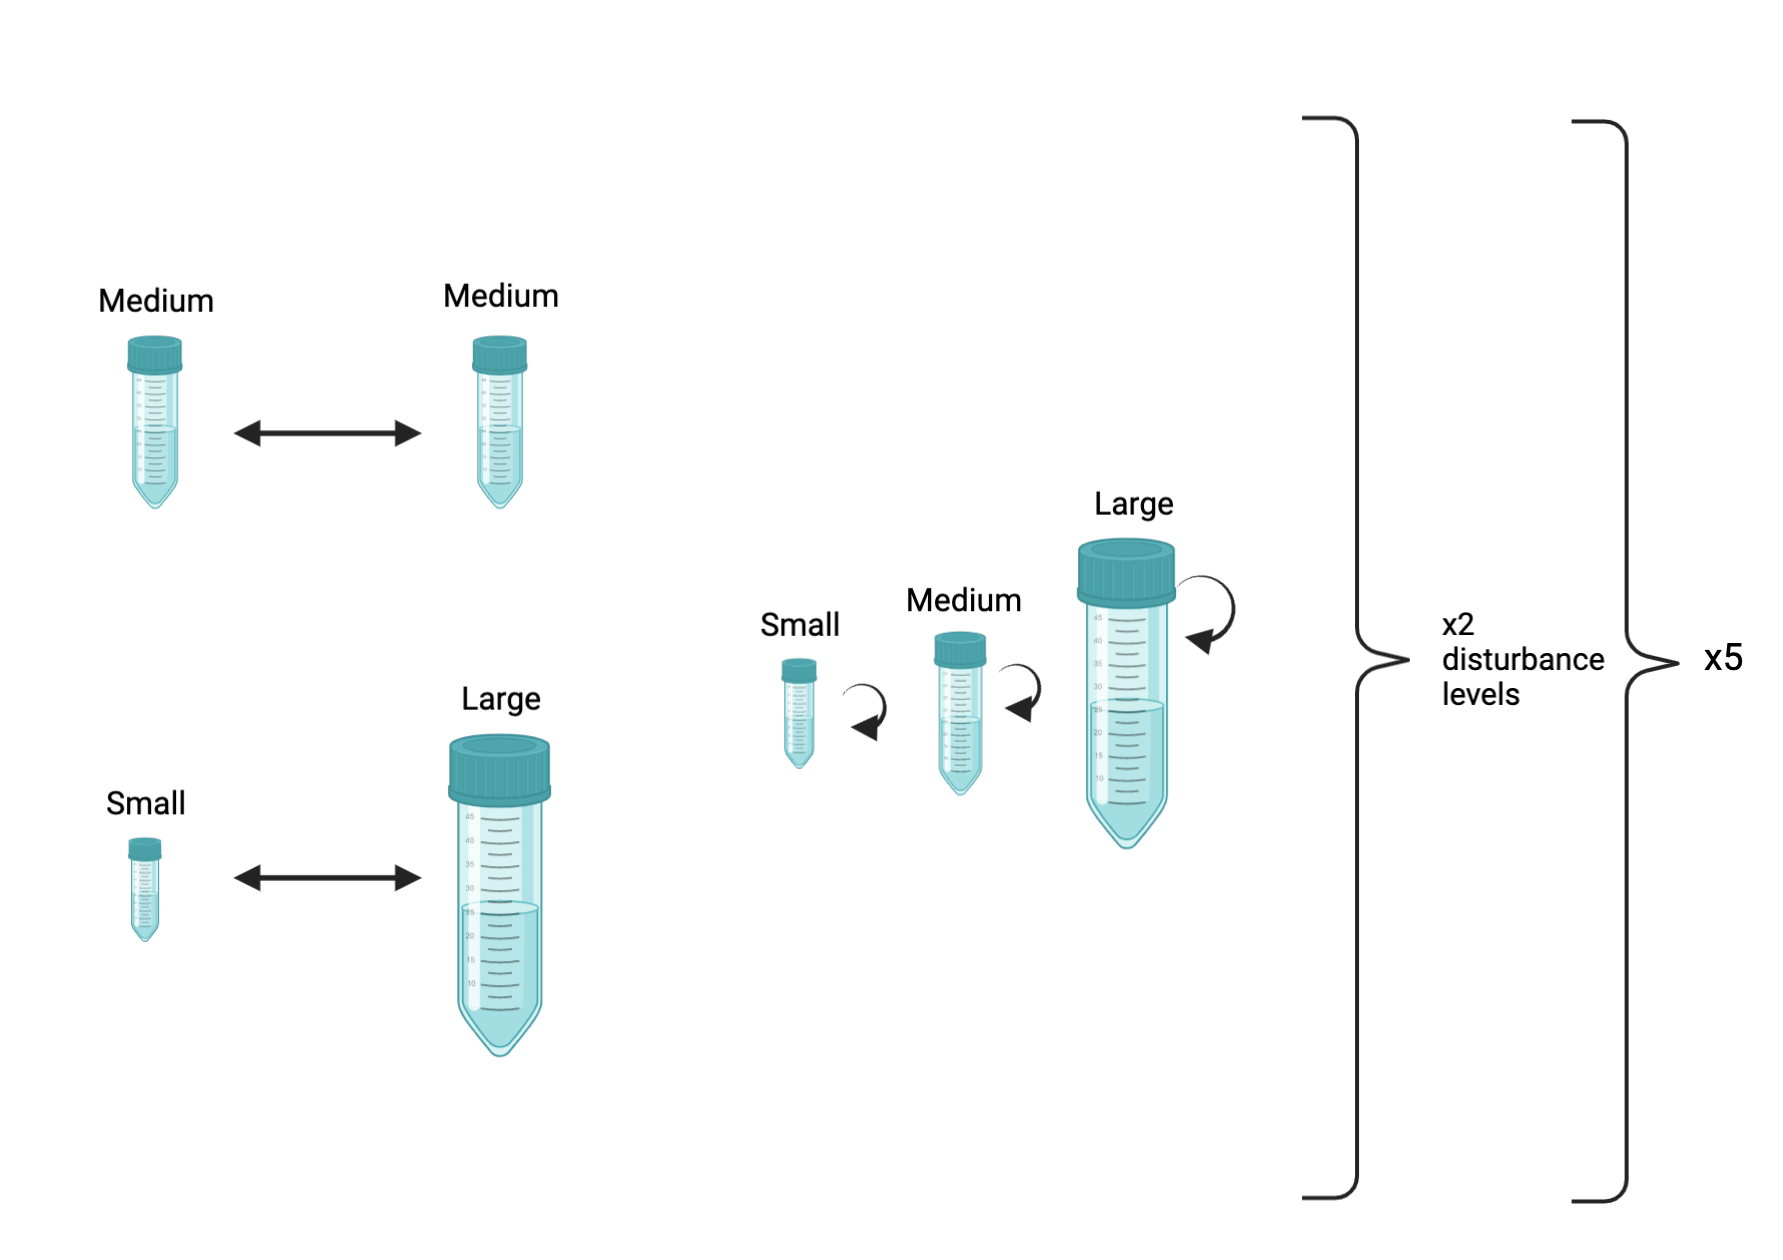
\includegraphics{images/Design.png}

\hypertarget{recap}{%
\subsubsection{Recap}\label{recap}}

Meta-ecosystems have been studied looking at meta-ecosystems in which
patch size was the same. However, of course, we know that
meta-ecosystems are mad out of patches that have different size. To see
the effects of patch size on meta-patch properties, we ran a four weeks
protist experiment in which different patches were connected through the
flow of nutrients. The flow of nutrients resulted from a perturbation of
the patches in which a fixed part of the cultures was boiled and then
poored into the receiving patch. This had a fixed volume (e.g., small
perturbation = 6.75 ml) and was the same across all patch sizes. The
experiment design consisted in crossing two disturbances with a small,
medium, and large isolated patches and with a small-small,
medium-medium, large-large, and small-large meta-patch. We took videos
every four days and we create this perturbation and resource flow the
day after taking videos. We skipped the perturbation the day after we
assembled the experiment so that we would start perturbing it when
population densities were already high.

We had mainly two research questions:

\begin{itemize}
\item
  Do patch properties of a patch depend upon the size of the patch it is
  connected to?
\item
  Do metaecosystem properties of a meta-patch depend upon the relative
  size of its patch?
\end{itemize}

\hypertarget{lab-work}{%
\subsubsection{Lab work}\label{lab-work}}

\hypertarget{creation-of-high-density-monocultures}{%
\paragraph{Creation of high-density
monocultures}\label{creation-of-high-density-monocultures}}

23/3/22 PPM for increasing the number of monocultures in the collection.

24/3/22 Collection control. See monoculture maintenance lab book p.~47.

26/3/22 Increase of number of monocultures in the collection. To do so,
take the best culture and make 3 new ones. See monoculture maintenance
lab book p.~47.

1/4/22 Make PPM for high density monocultures. See PatchSizePilot lab
book p.~5.

3/4/22 Make bacterial solution for high density monocultures. See
PatchSizePilot lab book p.~8.

5/4/22 Grow high density monocultures. Make 3 high density monocultures
for each protist species with 200 ml with 5\% bacterial solution, 85\%
PPM, 10\% protists, and 2 seeds. See PatchSizePilot lab book p.~10

10/4/2022 Check high density monocultures. Cep, Eup, Spi, Spi te were
really low.

13/4/2022 Start of the experiment. See PatchSizePilot p.~33.

\hypertarget{things-i-could-have-done-better}{%
\paragraph{Things I could have done
better}\label{things-i-could-have-done-better}}

- Autoclave all the material in advance

- Get more high-density monocultures

- Decide in advance the days in which you are going to check the
high-density monocultures and prepare bacteria in advance for that day
so that if some of them crashed you are still on time to make new ones.

- Use a single lab book for also when you create PPM and check the
collection.

- Make a really high amount of PPM, as you will need for so many
different things (\textgreater10 L). Maybe also autoclave 1 L Schott
bottles so that you don't have to oxygenate whole 5 L bottles of PPM. I
think that I should have maybe made even a 10 L bottle of PPM.

- According to Silvana protists take 4-7 days to grow. The fastest is
Tet (ca 4 days) and the slowest is Spi (ca 7 days). Once that you grow
them they should stay at carrying capacity for a bit of time I guess, as
you can see in the monoculture collection. I should make sure I'm
growing them in the right way. I think that maybe I should grow them 10
days in advance so that I could actually grow also the slow species if
they crashed. What should I do if all of them crashed?

\hypertarget{data}{%
\subsection{Data}\label{data}}

\hypertarget{experimental-cultures-culture_info}{%
\subsubsection{\texorpdfstring{Experimental cultures
(\texttt{culture\_info})}{Experimental cultures (culture\_info)}}\label{experimental-cultures-culture_info}}

This table contains information about the 110 cultures of the
experiment.

\begin{Shaded}
\begin{Highlighting}[]
\NormalTok{culture\_info }\OtherTok{=} \FunctionTok{read.csv}\NormalTok{(}\FunctionTok{here}\NormalTok{(}\StringTok{"data"}\NormalTok{, }\StringTok{"PatchSizePilot\_culture\_info.csv"}\NormalTok{), }\AttributeTok{header =} \ConstantTok{TRUE}\NormalTok{)}
\end{Highlighting}
\end{Shaded}

\hypertarget{individuals-ds_individuals}{%
\subsubsection{Individuals
(ds\_individuals)}\label{individuals-ds_individuals}}

\begin{Shaded}
\begin{Highlighting}[]
\NormalTok{ds\_individuals }\OtherTok{=} \FunctionTok{import.protist.morph.data}\NormalTok{(culture\_info,}
\NormalTok{                                           first\_time\_point,}
\NormalTok{                                           last\_time\_point)}
\end{Highlighting}
\end{Shaded}

\begin{Shaded}
\begin{Highlighting}[]
\CommentTok{\#Take off problematic videos}
\NormalTok{ds\_individuals\_before\_taking\_off\_videos }\OtherTok{=}\NormalTok{ ds\_individuals}

\NormalTok{ds\_individuals }\OtherTok{=}\NormalTok{ ds\_individuals }\SpecialCharTok{\%\textgreater{}\%}
  \FunctionTok{filter}\NormalTok{(}\SpecialCharTok{!}\NormalTok{(time\_point }\SpecialCharTok{\%in\%}\NormalTok{ videos\_to\_take\_off}\SpecialCharTok{$}\NormalTok{time\_point }\SpecialCharTok{\&} 
\NormalTok{           file }\SpecialCharTok{\%in\%}\NormalTok{ videos\_to\_take\_off}\SpecialCharTok{$}\NormalTok{file))}

\NormalTok{diff }\OtherTok{=} \FunctionTok{setdiff}\NormalTok{(ds\_individuals\_before\_taking\_off\_videos, ds\_individuals)}

\FunctionTok{expect\_equal}\NormalTok{(}\FunctionTok{nrow}\NormalTok{(videos\_to\_take\_off),}
             \FunctionTok{nrow}\NormalTok{(}\FunctionTok{expand.grid}\NormalTok{(diff}\SpecialCharTok{$}\NormalTok{culture\_ID, diff}\SpecialCharTok{$}\NormalTok{time\_point, diff}\SpecialCharTok{$}\NormalTok{file) }\SpecialCharTok{\%\textgreater{}\%} \FunctionTok{unique}\NormalTok{()))}

\CommentTok{\#Take off problematic cultures }
\NormalTok{ds\_individuals\_before\_taking\_off\_cultures }\OtherTok{=}\NormalTok{ ds\_individuals}

\NormalTok{ds\_individuals }\OtherTok{=}\NormalTok{ ds\_individuals }\SpecialCharTok{\%\textgreater{}\%}
  \FunctionTok{filter}\NormalTok{(}\SpecialCharTok{!}\NormalTok{ culture\_ID }\SpecialCharTok{\%in\%}\NormalTok{ patches\_to\_take\_off)}


\FunctionTok{expect\_equal}\NormalTok{(}\FunctionTok{setdiff}\NormalTok{(ds\_individuals\_before\_taking\_off\_cultures, ds\_individuals) }\SpecialCharTok{\%\textgreater{}\%} \FunctionTok{pull}\NormalTok{(culture\_ID) }\SpecialCharTok{\%\textgreater{}\%} \FunctionTok{unique}\NormalTok{(),}
\NormalTok{             patches\_to\_take\_off)}
\end{Highlighting}
\end{Shaded}

\begin{Shaded}
\begin{Highlighting}[]
\CommentTok{\#Rename columns}
\NormalTok{ds\_individuals }\OtherTok{=}\NormalTok{ ds\_individuals }\SpecialCharTok{\%\textgreater{}\%} 
  \FunctionTok{rename}\NormalTok{(}\AttributeTok{patch\_type =}\NormalTok{ eco\_metaeco\_type,}
         \AttributeTok{patch\_size\_ml =}\NormalTok{ patch\_size\_volume,}
\NormalTok{         body\_area\_µ}\AttributeTok{m2 =}\NormalTok{ mean\_area)}
\end{Highlighting}
\end{Shaded}

\begin{Shaded}
\begin{Highlighting}[]
\CommentTok{\#Rename the patches}
\NormalTok{ds\_individuals}\SpecialCharTok{$}\NormalTok{patch\_type[ds\_individuals}\SpecialCharTok{$}\NormalTok{patch\_type }\SpecialCharTok{==} \StringTok{"S"}\NormalTok{] }\OtherTok{=} \StringTok{"Small isolated"}
\NormalTok{ds\_individuals}\SpecialCharTok{$}\NormalTok{patch\_type[ds\_individuals}\SpecialCharTok{$}\NormalTok{patch\_type }\SpecialCharTok{==} \StringTok{"S (S\_S)"}\NormalTok{] }\OtherTok{=} \StringTok{"Small connected to small"}
\NormalTok{ds\_individuals}\SpecialCharTok{$}\NormalTok{patch\_type[ds\_individuals}\SpecialCharTok{$}\NormalTok{patch\_type }\SpecialCharTok{==} \StringTok{"S (S\_L)"}\NormalTok{] }\OtherTok{=} \StringTok{"Small connected to large"}
\NormalTok{ds\_individuals}\SpecialCharTok{$}\NormalTok{patch\_type[ds\_individuals}\SpecialCharTok{$}\NormalTok{patch\_type }\SpecialCharTok{==} \StringTok{"M"}\NormalTok{] }\OtherTok{=} \StringTok{"Medium isolated"}
\NormalTok{ds\_individuals}\SpecialCharTok{$}\NormalTok{patch\_type[ds\_individuals}\SpecialCharTok{$}\NormalTok{patch\_type }\SpecialCharTok{==} \StringTok{"M (M\_M)"}\NormalTok{] }\OtherTok{=} \StringTok{"Medium connected to medium"}
\NormalTok{ds\_individuals}\SpecialCharTok{$}\NormalTok{patch\_type[ds\_individuals}\SpecialCharTok{$}\NormalTok{patch\_type }\SpecialCharTok{==} \StringTok{"L"}\NormalTok{] }\OtherTok{=} \StringTok{"Large isolated"}
\NormalTok{ds\_individuals}\SpecialCharTok{$}\NormalTok{patch\_type[ds\_individuals}\SpecialCharTok{$}\NormalTok{patch\_type }\SpecialCharTok{==} \StringTok{"L (L\_L)"}\NormalTok{] }\OtherTok{=} \StringTok{"Large connected to large"}
\NormalTok{ds\_individuals}\SpecialCharTok{$}\NormalTok{patch\_type[ds\_individuals}\SpecialCharTok{$}\NormalTok{patch\_type }\SpecialCharTok{==} \StringTok{"L (S\_L)"}\NormalTok{] }\OtherTok{=} \StringTok{"Large connected to small"}

\CommentTok{\#Reorder the patches}
\NormalTok{ds\_individuals }\OtherTok{=}\NormalTok{ ds\_individuals }\SpecialCharTok{\%\textgreater{}\%}
  \FunctionTok{mutate}\NormalTok{(}\AttributeTok{patch\_type =} \FunctionTok{factor}\NormalTok{(}
\NormalTok{    patch\_type,}
    \AttributeTok{levels =} \FunctionTok{c}\NormalTok{(}
      \StringTok{"Small isolated"}\NormalTok{,}
      \StringTok{"Small connected to small"}\NormalTok{,}
      \StringTok{"Small connected to large"}\NormalTok{,}
      \StringTok{"Medium isolated"}\NormalTok{,}
      \StringTok{"Medium connected to medium"}\NormalTok{,}
      \StringTok{"Large isolated"}\NormalTok{,}
      \StringTok{"Large connected to large"}\NormalTok{,}
      \StringTok{"Large connected to small"}
\NormalTok{    )}
\NormalTok{  ))}
\end{Highlighting}
\end{Shaded}

\begin{Shaded}
\begin{Highlighting}[]
\CommentTok{\#Add the column size\_connected\_patch}
\NormalTok{ds\_individuals}\SpecialCharTok{$}\NormalTok{size\_connected\_patch }\OtherTok{=} \ConstantTok{NA}
\NormalTok{ds\_individuals}\SpecialCharTok{$}\NormalTok{size\_connected\_patch[ds\_individuals}\SpecialCharTok{$}\NormalTok{patch\_type }\SpecialCharTok{==} \StringTok{"Small connected to small"}\NormalTok{] }\OtherTok{=} \StringTok{"Small"}
\NormalTok{ds\_individuals}\SpecialCharTok{$}\NormalTok{size\_connected\_patch[ds\_individuals}\SpecialCharTok{$}\NormalTok{patch\_type }\SpecialCharTok{==} \StringTok{"Small connected to large"}\NormalTok{] }\OtherTok{=} \StringTok{"Large"}
\NormalTok{ds\_individuals}\SpecialCharTok{$}\NormalTok{size\_connected\_patch[ds\_individuals}\SpecialCharTok{$}\NormalTok{patch\_type }\SpecialCharTok{==} \StringTok{"Medium connected to medium"}\NormalTok{] }\OtherTok{=} \StringTok{"Medium"}
\NormalTok{ds\_individuals}\SpecialCharTok{$}\NormalTok{size\_connected\_patch[ds\_individuals}\SpecialCharTok{$}\NormalTok{patch\_type }\SpecialCharTok{==} \StringTok{"Large connected to large"}\NormalTok{] }\OtherTok{=} \StringTok{"Large"}
\NormalTok{ds\_individuals}\SpecialCharTok{$}\NormalTok{size\_connected\_patch[ds\_individuals}\SpecialCharTok{$}\NormalTok{patch\_type }\SpecialCharTok{==} \StringTok{"Large connected to small"}\NormalTok{] }\OtherTok{=} \StringTok{"Small"}
\end{Highlighting}
\end{Shaded}

\begin{Shaded}
\begin{Highlighting}[]
\CommentTok{\#Reorder columns}
\NormalTok{ds\_individuals }\OtherTok{=}\NormalTok{ ds\_individuals }\SpecialCharTok{\%\textgreater{}\%}
    \FunctionTok{select}\NormalTok{(time\_point,}
\NormalTok{           day, }
\NormalTok{           file, }
\NormalTok{           video\_replicate,}
\NormalTok{           disturbance, }
\NormalTok{           culture\_ID, }
\NormalTok{           system\_nr, }
\NormalTok{           patch\_type,}
\NormalTok{           patch\_size, }
\NormalTok{           patch\_size\_ml,}
\NormalTok{           size\_connected\_patch,}
\NormalTok{           metaecosystem, }
\NormalTok{           metaecosystem\_type, }
\NormalTok{           body\_area\_µm2,}
\NormalTok{           N\_frames}
\NormalTok{           )}
\end{Highlighting}
\end{Shaded}

\begin{Shaded}
\begin{Highlighting}[]
\FunctionTok{save}\NormalTok{(ds\_individuals, }\AttributeTok{file =} \FunctionTok{here}\NormalTok{(}\StringTok{"results"}\NormalTok{, }\StringTok{"ds"}\NormalTok{, }\StringTok{"ds\_individuals.RData"}\NormalTok{))}
\end{Highlighting}
\end{Shaded}

\hypertarget{patches-ds_patches}{%
\subsubsection{\texorpdfstring{Patches
(\texttt{ds\_patches})}{Patches (ds\_patches)}}\label{patches-ds_patches}}

After the dataset has been assembled

\begin{itemize}
\tightlist
\item
  Every row is a patch at a certain time point.
\item
  The value of different videos have been already averaged.
\end{itemize}

\begin{Shaded}
\begin{Highlighting}[]
\CommentTok{\#Assemble dataset (expected rows: sum(nr\_videos * n\_cultures))}
\NormalTok{ds\_patches }\OtherTok{=} \FunctionTok{import.protist.pop.data}\NormalTok{(culture\_info,}
\NormalTok{                                     first\_time\_point,}
\NormalTok{                                     last\_time\_point,}
\NormalTok{                                     protist\_species)}

\FunctionTok{expect\_equal}\NormalTok{(}\FunctionTok{nrow}\NormalTok{(ds\_patches), }
             \FunctionTok{sum}\NormalTok{(nr\_videos }\SpecialCharTok{*}\NormalTok{ n\_cultures))}
\end{Highlighting}
\end{Shaded}

\begin{Shaded}
\begin{Highlighting}[]
\CommentTok{\#Reorder dataset}
\NormalTok{ds\_patches }\OtherTok{=}\NormalTok{ ds\_patches }\SpecialCharTok{\%\textgreater{}\%}
  \FunctionTok{select}\NormalTok{(time\_point,}
\NormalTok{         day,}
\NormalTok{         file,}
\NormalTok{         video\_replicate,}
\NormalTok{         culture\_ID,}
\NormalTok{         system\_nr,}
\NormalTok{         disturbance,}
\NormalTok{         eco\_metaeco\_type,}
\NormalTok{         patch\_size,}
\NormalTok{         patch\_size\_volume,}
\NormalTok{         metaecosystem,}
\NormalTok{         metaecosystem\_type,}
\NormalTok{         bioarea\_per\_volume,}
         \FunctionTok{all\_of}\NormalTok{(protist\_species),}
\NormalTok{         Ble\_main\_analysis,}
\NormalTok{         Cep\_main\_analysis,}
\NormalTok{         Spi\_main\_analysis)}

\FunctionTok{expect\_equal}\NormalTok{(}\FunctionTok{nrow}\NormalTok{(ds\_patches), }
             \FunctionTok{sum}\NormalTok{(nr\_videos }\SpecialCharTok{*}\NormalTok{ n\_cultures))}
\end{Highlighting}
\end{Shaded}

\begin{Shaded}
\begin{Highlighting}[]
\CommentTok{\#Take off problematic videos}
\NormalTok{ds\_patches }\OtherTok{=}\NormalTok{ ds\_patches }\SpecialCharTok{\%\textgreater{}\%}
  \FunctionTok{filter}\NormalTok{(}\SpecialCharTok{!}\NormalTok{(time\_point }\SpecialCharTok{\%in\%}\NormalTok{ videos\_to\_take\_off}\SpecialCharTok{$}\NormalTok{time\_point }\SpecialCharTok{\&} 
\NormalTok{           file }\SpecialCharTok{\%in\%}\NormalTok{ videos\_to\_take\_off}\SpecialCharTok{$}\NormalTok{file))}

\FunctionTok{expect\_equal}\NormalTok{(}\FunctionTok{nrow}\NormalTok{(ds\_patches),}
             \FunctionTok{sum}\NormalTok{(nr\_videos }\SpecialCharTok{*}\NormalTok{ n\_cultures) }\SpecialCharTok{{-}} \FunctionTok{nrow}\NormalTok{(videos\_to\_take\_off))}

\CommentTok{\#Take off problematic cultures }
\NormalTok{ds\_patches }\OtherTok{=}\NormalTok{ ds\_patches }\SpecialCharTok{\%\textgreater{}\%}
  \FunctionTok{filter}\NormalTok{(}\SpecialCharTok{!}\NormalTok{ culture\_ID }\SpecialCharTok{\%in\%}\NormalTok{ patches\_to\_take\_off)}


\FunctionTok{expect\_equal}\NormalTok{(}\FunctionTok{nrow}\NormalTok{(ds\_patches),}
               \FunctionTok{sum}\NormalTok{(nr\_videos }\SpecialCharTok{*}\NormalTok{ n\_cultures) }\SpecialCharTok{{-}} \FunctionTok{nrow}\NormalTok{(videos\_to\_take\_off) }\SpecialCharTok{{-}}\NormalTok{ (}\FunctionTok{length}\NormalTok{(patches\_to\_take\_off) }\SpecialCharTok{*} \FunctionTok{sum}\NormalTok{(nr\_videos)))}

\ControlFlowTok{if}\NormalTok{(}\ConstantTok{TRUE} \SpecialCharTok{\%in\%} \FunctionTok{unique}\NormalTok{(videos\_to\_take\_off}\SpecialCharTok{$}\NormalTok{culture\_ID }\SpecialCharTok{==}\NormalTok{ patches\_to\_take\_off))\{}
  \FunctionTok{stop}\NormalTok{(}\StringTok{"Adjust your testing code, as the number of rows should consider that videos to take off are also in the patches to take off."}\NormalTok{)}
\NormalTok{\}}
\end{Highlighting}
\end{Shaded}

\begin{Shaded}
\begin{Highlighting}[]
\CommentTok{\#Rename columns}
\NormalTok{  ds\_patches }\OtherTok{=}\NormalTok{ ds\_patches }\SpecialCharTok{\%\textgreater{}\%}
    \FunctionTok{rename}\NormalTok{(}
      \AttributeTok{patch\_type =}\NormalTok{ eco\_metaeco\_type,}
\NormalTok{      bioarea\_µm2\_per\_μ}\AttributeTok{L =}\NormalTok{ bioarea\_per\_volume,}
      \AttributeTok{patch\_size\_ml =}\NormalTok{ patch\_size\_volume}
\NormalTok{    ) }\SpecialCharTok{\%\textgreater{}\%}
    \FunctionTok{rename\_with}\NormalTok{( }\SpecialCharTok{\textasciitilde{}} \FunctionTok{paste0}\NormalTok{(., }\StringTok{"\_indiv\_per\_μL"}\NormalTok{), }\FunctionTok{any\_of}\NormalTok{(}
      \FunctionTok{c}\NormalTok{(}
\NormalTok{        protist\_species,}
        \StringTok{"Ble\_low\_threshold\_analysis"}\NormalTok{,}
        \StringTok{"Cep\_low\_threshold\_analysis"}\NormalTok{,}
        \StringTok{"Spi\_low\_threshold\_analysis"}
\NormalTok{      )}
\NormalTok{    ))}

\CommentTok{\#Rename patches}
\NormalTok{ds\_patches}\SpecialCharTok{$}\NormalTok{patch\_type }\OtherTok{\textless{}{-}} \FunctionTok{recode}\NormalTok{(}
\NormalTok{  ds\_patches}\SpecialCharTok{$}\NormalTok{patch\_type,}
  \StringTok{"S"} \OtherTok{=} \StringTok{"Small isolated"}\NormalTok{,}
  \StringTok{"S (S\_S)"} \OtherTok{=} \StringTok{"Small connected to small"}\NormalTok{,}
  \StringTok{"S (S\_L)"} \OtherTok{=} \StringTok{"Small connected to large"}\NormalTok{,}
  \StringTok{"M"} \OtherTok{=} \StringTok{"Medium isolated"}\NormalTok{,}
  \StringTok{"M (M\_M)"} \OtherTok{=} \StringTok{"Medium connected to medium"}\NormalTok{,}
  \StringTok{"L"} \OtherTok{=} \StringTok{"Large isolated"}\NormalTok{,}
  \StringTok{"L (L\_L)"} \OtherTok{=} \StringTok{"Large connected to large"}\NormalTok{,}
  \StringTok{"L (S\_L)"} \OtherTok{=} \StringTok{"Large connected to small"}
\NormalTok{)}

\CommentTok{\#Rename patch sizes}
\NormalTok{ds\_patches}\SpecialCharTok{$}\NormalTok{patch\_size }\OtherTok{\textless{}{-}} \FunctionTok{recode}\NormalTok{(}
\NormalTok{  ds\_patches}\SpecialCharTok{$}\NormalTok{patch\_size,}
  \StringTok{"S"} \OtherTok{=} \StringTok{"Small"}\NormalTok{,}
  \StringTok{"M"} \OtherTok{=} \StringTok{"Medium"}\NormalTok{,}
  \StringTok{"L"} \OtherTok{=} \StringTok{"Large"}
\NormalTok{)}

\CommentTok{\#Rename the meta{-}ecosystems}
\NormalTok{ds\_patches}\SpecialCharTok{$}\NormalTok{metaecosystem\_type }\OtherTok{\textless{}{-}} \FunctionTok{recode}\NormalTok{(}
\NormalTok{  ds\_patches}\SpecialCharTok{$}\NormalTok{metaecosystem\_type,}
  \StringTok{"S\_S"} \OtherTok{=} \StringTok{"Small{-}Small meta{-}ecosystem"}\NormalTok{,}
  \StringTok{"M\_M"} \OtherTok{=} \StringTok{"Medium{-}Medium meta{-}ecosystem"}\NormalTok{,}
  \StringTok{"L\_L"} \OtherTok{=} \StringTok{"Large{-}Large meta{-}ecosystem"}\NormalTok{,}
  \StringTok{"S\_L"} \OtherTok{=} \StringTok{"Small{-}Large meta{-}ecosystem"}
\NormalTok{)}
\end{Highlighting}
\end{Shaded}

\begin{Shaded}
\begin{Highlighting}[]
\CommentTok{\#Reorder patches}
\NormalTok{ds\_patches }\OtherTok{=}\NormalTok{ ds\_patches }\SpecialCharTok{\%\textgreater{}\%}
  \FunctionTok{mutate}\NormalTok{(}\AttributeTok{patch\_type =} \FunctionTok{factor}\NormalTok{(}
\NormalTok{    patch\_type,}
    \AttributeTok{levels =} \FunctionTok{c}\NormalTok{(}
      \StringTok{"Small isolated"}\NormalTok{,}
      \StringTok{"Small connected to small"}\NormalTok{,}
      \StringTok{"Small connected to large"}\NormalTok{,}
      \StringTok{"Medium isolated"}\NormalTok{,}
      \StringTok{"Medium connected to medium"}\NormalTok{,}
      \StringTok{"Large isolated"}\NormalTok{,}
      \StringTok{"Large connected to large"}\NormalTok{,}
      \StringTok{"Large connected to small"}
\NormalTok{    )}
\NormalTok{  ))}

\CommentTok{\#Reorder the meta{-}ecosystems}
\NormalTok{ds\_patches }\OtherTok{=}\NormalTok{ ds\_patches }\SpecialCharTok{\%\textgreater{}\%}
  \FunctionTok{mutate}\NormalTok{(}\AttributeTok{metaecosystem\_type =} \FunctionTok{factor}\NormalTok{(}
\NormalTok{    metaecosystem\_type,}
    \AttributeTok{levels =} \FunctionTok{c}\NormalTok{(}
      \StringTok{"Small{-}Small meta{-}ecosystem"}\NormalTok{,}
      \StringTok{"Medium{-}Medium meta{-}ecosystem"}\NormalTok{,}
      \StringTok{"Medium{-}Medium isolated"}\NormalTok{,}
      \StringTok{"Large{-}Large meta{-}ecosystem"}\NormalTok{,}
      \StringTok{"Small{-}Large meta{-}ecosystem"}\NormalTok{,}
      \StringTok{"Small{-}Large isolated"}
\NormalTok{    )}
\NormalTok{  ))}
\end{Highlighting}
\end{Shaded}

\begin{Shaded}
\begin{Highlighting}[]
\CommentTok{\#Add the column size\_connected\_patch}
\NormalTok{ds\_patches}\SpecialCharTok{$}\NormalTok{size\_connected\_patch }\OtherTok{=} \ConstantTok{NA}
\NormalTok{ds\_patches}\SpecialCharTok{$}\NormalTok{size\_connected\_patch[ds\_patches}\SpecialCharTok{$}\NormalTok{patch\_type }\SpecialCharTok{==} \StringTok{"Small connected to small"}\NormalTok{] }\OtherTok{=} \StringTok{"Small"}
\NormalTok{ds\_patches}\SpecialCharTok{$}\NormalTok{size\_connected\_patch[ds\_patches}\SpecialCharTok{$}\NormalTok{patch\_type }\SpecialCharTok{==} \StringTok{"Small connected to large"}\NormalTok{] }\OtherTok{=} \StringTok{"Large"}
\NormalTok{ds\_patches}\SpecialCharTok{$}\NormalTok{size\_connected\_patch[ds\_patches}\SpecialCharTok{$}\NormalTok{patch\_type }\SpecialCharTok{==} \StringTok{"Medium connected to medium"}\NormalTok{] }\OtherTok{=} \StringTok{"Medium"}
\NormalTok{ds\_patches}\SpecialCharTok{$}\NormalTok{size\_connected\_patch[ds\_patches}\SpecialCharTok{$}\NormalTok{patch\_type }\SpecialCharTok{==} \StringTok{"Large connected to large"}\NormalTok{] }\OtherTok{=} \StringTok{"Large"}
\NormalTok{ds\_patches}\SpecialCharTok{$}\NormalTok{size\_connected\_patch[ds\_patches}\SpecialCharTok{$}\NormalTok{patch\_type }\SpecialCharTok{==} \StringTok{"Large connected to small"}\NormalTok{] }\OtherTok{=} \StringTok{"Small"}

\CommentTok{\#Change all the measures to ml}
\NormalTok{ds\_patches }\OtherTok{=}\NormalTok{ ds\_patches }\SpecialCharTok{\%\textgreater{}\%}
  \FunctionTok{mutate}\NormalTok{(bioarea\_µ}\AttributeTok{m2\_per\_ml =}\NormalTok{ bioarea\_µm2\_per\_μL }\SpecialCharTok{*}\NormalTok{ (}\DecValTok{10}\SpecialCharTok{\^{}}\DecValTok{3}\NormalTok{),}
         \AttributeTok{bioarea\_mm2\_per\_ml =}\NormalTok{ bioarea\_µm2\_per\_ml }\SpecialCharTok{/}\NormalTok{ (}\DecValTok{10}\SpecialCharTok{\^{}}\DecValTok{6}\NormalTok{),}
         \AttributeTok{Ble\_indiv\_per\_ml =}\NormalTok{ Ble\_indiv\_per\_μL }\SpecialCharTok{*}\NormalTok{ (}\DecValTok{10}\SpecialCharTok{\^{}}\DecValTok{3}\NormalTok{),}
         \AttributeTok{Cep\_indiv\_per\_ml =}\NormalTok{ Cep\_indiv\_per\_μL }\SpecialCharTok{*}\NormalTok{ (}\DecValTok{10}\SpecialCharTok{\^{}}\DecValTok{3}\NormalTok{),}
         \AttributeTok{Col\_indiv\_per\_ml =}\NormalTok{ Col\_indiv\_per\_μL }\SpecialCharTok{*}\NormalTok{ (}\DecValTok{10}\SpecialCharTok{\^{}}\DecValTok{3}\NormalTok{),}
         \AttributeTok{Eug\_indiv\_per\_ml =}\NormalTok{ Eug\_indiv\_per\_μL }\SpecialCharTok{*}\NormalTok{ (}\DecValTok{10}\SpecialCharTok{\^{}}\DecValTok{3}\NormalTok{),}
         \AttributeTok{Eup\_indiv\_per\_ml =}\NormalTok{ Eup\_indiv\_per\_μL }\SpecialCharTok{*}\NormalTok{ (}\DecValTok{10}\SpecialCharTok{\^{}}\DecValTok{3}\NormalTok{),}
         \AttributeTok{Lox\_indiv\_per\_ml =}\NormalTok{ Lox\_indiv\_per\_μL }\SpecialCharTok{*}\NormalTok{ (}\DecValTok{10}\SpecialCharTok{\^{}}\DecValTok{3}\NormalTok{),}
         \AttributeTok{Pau\_indiv\_per\_ml =}\NormalTok{ Pau\_indiv\_per\_μL }\SpecialCharTok{*}\NormalTok{ (}\DecValTok{10}\SpecialCharTok{\^{}}\DecValTok{3}\NormalTok{),}
         \AttributeTok{Pca\_indiv\_per\_ml =}\NormalTok{ Pca\_indiv\_per\_μL }\SpecialCharTok{*}\NormalTok{ (}\DecValTok{10}\SpecialCharTok{\^{}}\DecValTok{3}\NormalTok{),}
         \AttributeTok{Spi\_indiv\_per\_ml =}\NormalTok{ Spi\_indiv\_per\_μL }\SpecialCharTok{*}\NormalTok{ (}\DecValTok{10}\SpecialCharTok{\^{}}\DecValTok{3}\NormalTok{),}
         \AttributeTok{Spi\_te\_indiv\_per\_ml =}\NormalTok{ Spi\_te\_indiv\_per\_μL }\SpecialCharTok{*}\NormalTok{ (}\DecValTok{10}\SpecialCharTok{\^{}}\DecValTok{3}\NormalTok{),}
         \AttributeTok{Tet\_indiv\_per\_ml =}\NormalTok{ Tet\_indiv\_per\_μL }\SpecialCharTok{*}\NormalTok{ (}\DecValTok{10}\SpecialCharTok{\^{}}\DecValTok{3}\NormalTok{))}
\end{Highlighting}
\end{Shaded}

\begin{Shaded}
\begin{Highlighting}[]
\CommentTok{\#Rearrange}
\NormalTok{ds\_patches }\OtherTok{=}\NormalTok{ ds\_patches }\SpecialCharTok{\%\textgreater{}\%}
  \FunctionTok{select}\NormalTok{(time\_point,}
\NormalTok{         day,}
\NormalTok{         file,}
\NormalTok{         video\_replicate,}
\NormalTok{         culture\_ID,}
\NormalTok{         system\_nr,}
\NormalTok{         disturbance,}
\NormalTok{         patch\_type,}
\NormalTok{         patch\_size,}
\NormalTok{         patch\_size\_ml,}
\NormalTok{         size\_connected\_patch,}
\NormalTok{         metaecosystem,}
\NormalTok{         metaecosystem\_type,}
\NormalTok{         bioarea\_mm2\_per\_ml,}
         \FunctionTok{all\_of}\NormalTok{(protist\_species\_indiv\_per\_ml))}
\end{Highlighting}
\end{Shaded}

\begin{Shaded}
\begin{Highlighting}[]
\DocumentationTok{\#\#\# Average videos}
\NormalTok{ds\_patches }\OtherTok{=}\NormalTok{ ds\_patches }\SpecialCharTok{\%\textgreater{}\%}
  \FunctionTok{group\_by}\NormalTok{(}\FunctionTok{across}\NormalTok{(}\FunctionTok{all\_of}\NormalTok{(columns\_patches))) }\SpecialCharTok{\%\textgreater{}\%}
  \FunctionTok{summarise}\NormalTok{(}\FunctionTok{across}\NormalTok{(}\FunctionTok{contains}\NormalTok{(}\StringTok{"\_per\_ml"}\NormalTok{), mean),}
            \FunctionTok{across}\NormalTok{(}\FunctionTok{contains}\NormalTok{(}\StringTok{"\_tot"}\NormalTok{), mean)) }\SpecialCharTok{\%\textgreater{}\%}
  \FunctionTok{ungroup}\NormalTok{()}

\FunctionTok{expect\_equal}\NormalTok{(}\FunctionTok{nrow}\NormalTok{(ds\_patches),}
\NormalTok{             (n\_cultures }\SpecialCharTok{{-}} \FunctionTok{length}\NormalTok{(patches\_to\_take\_off)) }\SpecialCharTok{*} \FunctionTok{length}\NormalTok{(time\_points))}
\end{Highlighting}
\end{Shaded}

\begin{Shaded}
\begin{Highlighting}[]
\CommentTok{\#Calculate individuals per ml (based on a combination of the two analyses). }
\NormalTok{ds\_patches }\OtherTok{=}\NormalTok{ ds\_patches }\SpecialCharTok{\%\textgreater{}\%}
  \FunctionTok{mutate}\NormalTok{(}\AttributeTok{indiv\_per\_ml =} \SpecialCharTok{!!}\NormalTok{rlang}\SpecialCharTok{::}\FunctionTok{parse\_expr}\NormalTok{(}\FunctionTok{paste}\NormalTok{(}\FunctionTok{paste0}\NormalTok{(protist\_species, }\StringTok{"\_indiv\_per\_ml"}\NormalTok{), }\AttributeTok{collapse =} \StringTok{" + "}\NormalTok{)))}

\CommentTok{\#Calculate total response variable for the whole patch}
\NormalTok{ds\_patches }\OtherTok{=}\NormalTok{ ds\_patches }\SpecialCharTok{\%\textgreater{}\%}
  \FunctionTok{mutate}\NormalTok{(}\AttributeTok{bioarea\_tot\_mm2 =}\NormalTok{ bioarea\_mm2\_per\_ml }\SpecialCharTok{*}\NormalTok{ patch\_size\_ml,}
         \AttributeTok{indiv\_tot =}\NormalTok{ indiv\_per\_ml }\SpecialCharTok{*}\NormalTok{ patch\_size\_ml,}
         \AttributeTok{Ble\_tot\_indiv =}\NormalTok{ Ble\_indiv\_per\_ml }\SpecialCharTok{*}\NormalTok{ patch\_size\_ml,}
         \AttributeTok{Cep\_tot\_indiv =}\NormalTok{ Cep\_indiv\_per\_ml }\SpecialCharTok{*}\NormalTok{ patch\_size\_ml,}
         \AttributeTok{Col\_tot\_indiv =}\NormalTok{ Col\_indiv\_per\_ml }\SpecialCharTok{*}\NormalTok{ patch\_size\_ml,}
         \AttributeTok{Eug\_tot\_indiv =}\NormalTok{ Eug\_indiv\_per\_ml }\SpecialCharTok{*}\NormalTok{ patch\_size\_ml,}
         \AttributeTok{Eup\_tot\_indiv =}\NormalTok{ Eup\_indiv\_per\_ml }\SpecialCharTok{*}\NormalTok{ patch\_size\_ml,}
         \AttributeTok{Lox\_tot\_indiv =}\NormalTok{ Lox\_indiv\_per\_ml }\SpecialCharTok{*}\NormalTok{ patch\_size\_ml,}
         \AttributeTok{Pau\_tot\_indiv =}\NormalTok{ Pau\_indiv\_per\_ml }\SpecialCharTok{*}\NormalTok{ patch\_size\_ml,}
         \AttributeTok{Pca\_tot\_indiv =}\NormalTok{ Pca\_indiv\_per\_ml }\SpecialCharTok{*}\NormalTok{ patch\_size\_ml,}
         \AttributeTok{Spi\_tot\_indiv =}\NormalTok{ Spi\_indiv\_per\_ml }\SpecialCharTok{*}\NormalTok{ patch\_size\_ml,}
         \AttributeTok{Spi\_te\_tot\_indiv =}\NormalTok{ Spi\_te\_indiv\_per\_ml }\SpecialCharTok{*}\NormalTok{ patch\_size\_ml,}
         \AttributeTok{Tet\_tot\_indiv =}\NormalTok{ Tet\_indiv\_per\_ml }\SpecialCharTok{*}\NormalTok{ patch\_size\_ml)}


\CommentTok{\#Calculate species dominance}
\NormalTok{ds\_patches }\OtherTok{=}\NormalTok{ ds\_patches }\SpecialCharTok{\%\textgreater{}\%}
  \FunctionTok{mutate}\NormalTok{(}\FunctionTok{across}\NormalTok{(}\FunctionTok{all\_of}\NormalTok{(protist\_species\_indiv\_per\_ml), }
                \FunctionTok{list}\NormalTok{(}\AttributeTok{dominance =} \SpecialCharTok{\textasciitilde{}}\NormalTok{ (. }\SpecialCharTok{/}\NormalTok{ indiv\_per\_ml) }\SpecialCharTok{*} \DecValTok{100}\NormalTok{), }
                \AttributeTok{.names =} \StringTok{"\{col\}\_dominance"}\NormalTok{))}

\FunctionTok{expect\_equal}\NormalTok{(}\FunctionTok{unique}\NormalTok{(ds\_patches}\SpecialCharTok{$}\NormalTok{Ble\_indiv\_per\_ml\_dominance[ds\_patches}\SpecialCharTok{$}\NormalTok{indiv\_per\_ml }\SpecialCharTok{==} \DecValTok{0}\NormalTok{]),}
             \ConstantTok{NaN}\NormalTok{)}
\end{Highlighting}
\end{Shaded}

\begin{Shaded}
\begin{Highlighting}[]
\NormalTok{n\_rows\_ds\_patches\_before\_calculations }\OtherTok{=} \FunctionTok{nrow}\NormalTok{(ds\_patches)}
\end{Highlighting}
\end{Shaded}

\begin{Shaded}
\begin{Highlighting}[]
\CommentTok{\#Calculate alpha diversity.}
\CommentTok{\#This includes shannon, simpson, inv simpson, evenness.}
\NormalTok{ds\_patches }\OtherTok{=} \FunctionTok{calculate.alpha.diversity}\NormalTok{()}

\CommentTok{\#I\textquotesingle{}m not sure why this is not already done automatically in the previous step }
\NormalTok{ds\_patches}\SpecialCharTok{$}\NormalTok{shannon[ds\_patches}\SpecialCharTok{$}\NormalTok{species\_richness }\SpecialCharTok{==} \DecValTok{1}\NormalTok{] }\OtherTok{=} \DecValTok{0}

\FunctionTok{expect\_equal}\NormalTok{(}\FunctionTok{max}\NormalTok{(ds\_patches}\SpecialCharTok{$}\NormalTok{species\_richness),}
\NormalTok{             n\_protist\_species)}
\end{Highlighting}
\end{Shaded}

\begin{Shaded}
\begin{Highlighting}[]
\CommentTok{\#Calculate divergence from isolated. }
\CommentTok{\#This is the difference in community composition of each culture from the other isolated cultures (Bray{-}Curtis). The warning appears because in some cases we are comparing with a communities that has completely crashed and so Bray{-}Curtis is 1.}
\NormalTok{ds\_patches }\OtherTok{=} \FunctionTok{calculate.treatment.divergence}\NormalTok{()}

\FunctionTok{expect\_true}\NormalTok{(}\FunctionTok{max}\NormalTok{(ds\_patches}\SpecialCharTok{$}\NormalTok{beta\_diversity\_from\_isolated, }\AttributeTok{na.rm =}\NormalTok{ T) }\SpecialCharTok{\textless{}=} \DecValTok{1}\NormalTok{)}
\FunctionTok{expect\_true}\NormalTok{(}\FunctionTok{min}\NormalTok{(ds\_patches}\SpecialCharTok{$}\NormalTok{beta\_diversity\_from\_isolated, }\AttributeTok{na.rm =}\NormalTok{ T) }\SpecialCharTok{\textgreater{}=} \DecValTok{0}\NormalTok{)}

\FunctionTok{saveRDS}\NormalTok{(ds\_patches, }\AttributeTok{file =} \FunctionTok{here}\NormalTok{(}\StringTok{"results"}\NormalTok{, }\StringTok{"ds\_patches\_w\_treatment\_divergence.RData"}\NormalTok{))}
\end{Highlighting}
\end{Shaded}

\begin{Shaded}
\begin{Highlighting}[]
\NormalTok{ds\_patches }\OtherTok{=} \FunctionTok{readRDS}\NormalTok{(}\FunctionTok{here}\NormalTok{(}\StringTok{"results"}\NormalTok{, }\StringTok{"ds\_patches\_w\_treatment\_divergence.RData"}\NormalTok{))}
\end{Highlighting}
\end{Shaded}

Warning appear after the following code, as beta diversity is computed
for a culture between when it totally crashed and its previous time
point. Because the culture is totally crashed, the Bray-Curtis index is
1.

\begin{Shaded}
\begin{Highlighting}[]
\CommentTok{\#Calculate temporal divergence. }
\CommentTok{\#This is the difference in community composition of each culture from its previous time point (Bray{-}Curtis).}
\NormalTok{ds\_patches }\OtherTok{=} \FunctionTok{calculate.temporal.divergence}\NormalTok{()}
\end{Highlighting}
\end{Shaded}

\begin{verbatim}
## Warning in vegdist(., method = "bray"): you have empty rows: their dissimilarities may be
##                  meaningless in method "bray"

## Warning in vegdist(., method = "bray"): you have empty rows: their dissimilarities may be
##                  meaningless in method "bray"

## Warning in vegdist(., method = "bray"): you have empty rows: their dissimilarities may be
##                  meaningless in method "bray"

## Warning in vegdist(., method = "bray"): you have empty rows: their dissimilarities may be
##                  meaningless in method "bray"

## Warning in vegdist(., method = "bray"): you have empty rows: their dissimilarities may be
##                  meaningless in method "bray"

## Warning in vegdist(., method = "bray"): you have empty rows: their dissimilarities may be
##                  meaningless in method "bray"

## Warning in vegdist(., method = "bray"): you have empty rows: their dissimilarities may be
##                  meaningless in method "bray"

## Warning in vegdist(., method = "bray"): you have empty rows: their dissimilarities may be
##                  meaningless in method "bray"
\end{verbatim}

\begin{verbatim}
## Warning in vegdist(., method = "bray"): missing values in results
\end{verbatim}

\begin{verbatim}
## Warning in vegdist(., method = "bray"): you have empty rows: their dissimilarities may be
##                  meaningless in method "bray"

## Warning in vegdist(., method = "bray"): you have empty rows: their dissimilarities may be
##                  meaningless in method "bray"

## Warning in vegdist(., method = "bray"): you have empty rows: their dissimilarities may be
##                  meaningless in method "bray"

## Warning in vegdist(., method = "bray"): you have empty rows: their dissimilarities may be
##                  meaningless in method "bray"

## Warning in vegdist(., method = "bray"): you have empty rows: their dissimilarities may be
##                  meaningless in method "bray"

## Warning in vegdist(., method = "bray"): you have empty rows: their dissimilarities may be
##                  meaningless in method "bray"

## Warning in vegdist(., method = "bray"): you have empty rows: their dissimilarities may be
##                  meaningless in method "bray"

## Warning in vegdist(., method = "bray"): you have empty rows: their dissimilarities may be
##                  meaningless in method "bray"
\end{verbatim}

\begin{Shaded}
\begin{Highlighting}[]
\FunctionTok{expect\_true}\NormalTok{(}\FunctionTok{max}\NormalTok{(ds\_patches}\SpecialCharTok{$}\NormalTok{beta\_diversity\_from\_previous\_time, }\AttributeTok{na.rm =}\NormalTok{ T) }\SpecialCharTok{\textless{}=} \DecValTok{1}\NormalTok{)}
\FunctionTok{expect\_true}\NormalTok{(}\FunctionTok{min}\NormalTok{(ds\_patches}\SpecialCharTok{$}\NormalTok{beta\_diversity\_from\_previous\_time, }\AttributeTok{na.rm =}\NormalTok{ T) }\SpecialCharTok{\textgreater{}=} \DecValTok{0}\NormalTok{)}
\end{Highlighting}
\end{Shaded}

\begin{Shaded}
\begin{Highlighting}[]
\CommentTok{\#Calculate median body size}
\NormalTok{ds\_median\_body\_size }\OtherTok{=}\NormalTok{ ds\_individuals }\SpecialCharTok{\%\textgreater{}\%}
  \FunctionTok{group\_by}\NormalTok{(time\_point,}
\NormalTok{           culture\_ID,}
\NormalTok{           file) }\SpecialCharTok{\%\textgreater{}\%}
  \FunctionTok{summarise}\NormalTok{(median\_body\_area\_µ}\AttributeTok{m2 =} \FunctionTok{median}\NormalTok{(body\_area\_µm2)) }\SpecialCharTok{\%\textgreater{}\%}
  \FunctionTok{group\_by}\NormalTok{(time\_point,}
\NormalTok{           culture\_ID) }\SpecialCharTok{\%\textgreater{}\%}
  \FunctionTok{summarise}\NormalTok{(median\_body\_area\_µ}\AttributeTok{m2 =} \FunctionTok{mean}\NormalTok{(median\_body\_area\_µm2))}

\FunctionTok{expect\_true}\NormalTok{(}\FunctionTok{nrow}\NormalTok{(ds\_median\_body\_size) }\SpecialCharTok{\textless{}=} \FunctionTok{nrow}\NormalTok{(ds\_patches))}

\NormalTok{ds\_patches }\OtherTok{=} \FunctionTok{full\_join}\NormalTok{(ds\_patches, ds\_median\_body\_size)}

\FunctionTok{expect\_equal}\NormalTok{(}\FunctionTok{nrow}\NormalTok{(ds\_patches),}
\NormalTok{             n\_rows\_ds\_patches\_before\_calculations)}
\end{Highlighting}
\end{Shaded}

\begin{Shaded}
\begin{Highlighting}[]
\CommentTok{\#Calculate baselines. }
\CommentTok{\#To consider the initial values for different cultures when analyzing their temporal trends, we add baselines from time point 1. These baselines are used because at time point 0, we only measured the community of the large bottle that the experiment was assembled from. Additionally, the first perturbation had already occurred by time point 2, which is the starting point for our models.}
\NormalTok{baselines }\OtherTok{\textless{}{-}}\NormalTok{ ds\_patches }\SpecialCharTok{\%\textgreater{}\%}
  \FunctionTok{filter}\NormalTok{(time\_point }\SpecialCharTok{==} \DecValTok{1}\NormalTok{) }\SpecialCharTok{\%\textgreater{}\%}
  \FunctionTok{group\_by}\NormalTok{(culture\_ID) }\SpecialCharTok{\%\textgreater{}\%}
  \FunctionTok{summarise}\NormalTok{(}\FunctionTok{across}\NormalTok{(}\FunctionTok{all\_of}\NormalTok{(variables\_patches), }
                   \AttributeTok{.names =} \StringTok{"baseline\_\{.col\}"}\NormalTok{))}

\NormalTok{ds\_patches }\OtherTok{=} \FunctionTok{full\_join}\NormalTok{(ds\_patches, baselines)}

\FunctionTok{expect\_equal}\NormalTok{(}\FunctionTok{nrow}\NormalTok{(ds\_patches),}
\NormalTok{             n\_rows\_ds\_patches\_before\_calculations)}
\end{Highlighting}
\end{Shaded}

\begin{Shaded}
\begin{Highlighting}[]
\CommentTok{\#Finalise the dataset by arranging the columns in the order that makes the most sense.}
\NormalTok{ds\_patches }\OtherTok{=}\NormalTok{ ds\_patches }\SpecialCharTok{\%\textgreater{}\%}
  \FunctionTok{select}\NormalTok{(}\FunctionTok{any\_of}\NormalTok{(}\FunctionTok{c}\NormalTok{(}
\NormalTok{    columns\_patches,}
\NormalTok{    variables\_patches,}
\NormalTok{    baseline\_columns}
\NormalTok{  )))}
\end{Highlighting}
\end{Shaded}

\begin{Shaded}
\begin{Highlighting}[]
\FunctionTok{save}\NormalTok{(ds\_patches, }\AttributeTok{file =} \FunctionTok{here}\NormalTok{(}\StringTok{"results"}\NormalTok{, }\StringTok{"ds"}\NormalTok{, }\StringTok{"ds\_patches.RData"}\NormalTok{))}
\end{Highlighting}
\end{Shaded}

\hypertarget{patch-effect-sizes-ds_patches_effect_size}{%
\subsubsection{\texorpdfstring{Patch effect sizes
(\texttt{ds\_patches\_effect\_size})}{Patch effect sizes (ds\_patches\_effect\_size)}}\label{patch-effect-sizes-ds_patches_effect_size}}

\begin{Shaded}
\begin{Highlighting}[]
\NormalTok{vars\_to\_group\_by }\OtherTok{=}\NormalTok{ columns\_patches[columns\_patches }\SpecialCharTok{!=} \StringTok{"culture\_ID"} \SpecialCharTok{\&}\NormalTok{ columns\_patches }\SpecialCharTok{!=} \StringTok{"system\_nr"}\NormalTok{]}

\NormalTok{ds\_patches\_effect\_size }\OtherTok{=} \FunctionTok{calculate.effect.sizes}\NormalTok{(ds\_patches,}
\NormalTok{                                                vars\_to\_group\_by,}
\NormalTok{                                                variables\_patches) }\SpecialCharTok{\%\textgreater{}\%}
  \FunctionTok{filter}\NormalTok{(time\_point }\SpecialCharTok{\textgreater{}=} \DecValTok{1}\NormalTok{)}
\end{Highlighting}
\end{Shaded}

\begin{verbatim}
## Warning: Using `all_of()` outside of a selecting function was deprecated in tidyselect
## 1.2.0.
## i See details at
##   <https://tidyselect.r-lib.org/reference/faq-selection-context.html>
\end{verbatim}

\begin{Shaded}
\begin{Highlighting}[]
\FunctionTok{expect\_equal}\NormalTok{(}\FunctionTok{nrow}\NormalTok{(ds\_patches\_effect\_size), }
\NormalTok{             (n\_treatments }\SpecialCharTok{+}\NormalTok{ n\_controls) }\SpecialCharTok{*}\NormalTok{ (n\_time\_points }\SpecialCharTok{{-}} \DecValTok{1}\NormalTok{) }\SpecialCharTok{*}\NormalTok{ n\_disturbance\_levels)}
\end{Highlighting}
\end{Shaded}

\begin{Shaded}
\begin{Highlighting}[]
\CommentTok{\#Add baselines (from t1).}
\NormalTok{baselines }\OtherTok{\textless{}{-}}\NormalTok{ ds\_patches\_effect\_size }\SpecialCharTok{\%\textgreater{}\%}
  \FunctionTok{filter}\NormalTok{(time\_point }\SpecialCharTok{==} \DecValTok{1}\NormalTok{) }\SpecialCharTok{\%\textgreater{}\%}
  \FunctionTok{group\_by}\NormalTok{(patch\_type, disturbance) }\SpecialCharTok{\%\textgreater{}\%}
  \FunctionTok{summarise}\NormalTok{(}\FunctionTok{across}\NormalTok{(}\FunctionTok{paste0}\NormalTok{(variables\_patches, }\StringTok{"\_d"}\NormalTok{), }
                   \AttributeTok{.names =} \StringTok{"baseline\_\{.col\}"}\NormalTok{)) }\SpecialCharTok{\%\textgreater{}\%}
  \FunctionTok{select}\NormalTok{(patch\_type,}
\NormalTok{         disturbance,}
         \FunctionTok{paste0}\NormalTok{(}\StringTok{"baseline\_"}\NormalTok{, variables\_patches, }\StringTok{"\_d"}\NormalTok{))}


\FunctionTok{expect\_equal}\NormalTok{(}\FunctionTok{nrow}\NormalTok{(baselines), }
\NormalTok{             (n\_treatments }\SpecialCharTok{+}\NormalTok{ n\_controls) }\SpecialCharTok{*}\NormalTok{ n\_disturbance\_levels)}

\NormalTok{n\_rows\_ds\_patches\_ES\_before\_joining\_baselines }\OtherTok{=} \FunctionTok{nrow}\NormalTok{(ds\_patches\_effect\_size)}

\NormalTok{ds\_patches\_effect\_size }\OtherTok{=} \FunctionTok{full\_join}\NormalTok{(ds\_patches\_effect\_size, baselines)}

\FunctionTok{expect\_equal}\NormalTok{(n\_rows\_ds\_patches\_ES\_before\_joining\_baselines, }
               \FunctionTok{nrow}\NormalTok{(ds\_patches\_effect\_size))}
\end{Highlighting}
\end{Shaded}

\begin{Shaded}
\begin{Highlighting}[]
\FunctionTok{save}\NormalTok{(ds\_patches\_effect\_size, }\AttributeTok{file =} \FunctionTok{here}\NormalTok{(}\StringTok{"results"}\NormalTok{, }\StringTok{"ds"}\NormalTok{, }\StringTok{"ds\_patches\_effect\_size.RData"}\NormalTok{))}
\end{Highlighting}
\end{Shaded}

\hypertarget{meta-ecosystems-ds_metaecosystems}{%
\subsubsection{\texorpdfstring{Meta-ecosystems
(\texttt{ds\_metaecosystems})}{Meta-ecosystems (ds\_metaecosystems)}}\label{meta-ecosystems-ds_metaecosystems}}

\begin{Shaded}
\begin{Highlighting}[]
\DocumentationTok{\#\#\# Create a data frame with all the experimental meta{-}ecosystems and all the possible meta{-}ecosystems from isolated}
\NormalTok{culture\_ID\_isolated\_S\_low }\OtherTok{=}\NormalTok{ ds\_patches }\SpecialCharTok{\%\textgreater{}\%}
  \FunctionTok{filter}\NormalTok{(patch\_type }\SpecialCharTok{==} \StringTok{"Small isolated"}\NormalTok{,}
\NormalTok{         disturbance }\SpecialCharTok{==} \StringTok{"low"}\NormalTok{) }\SpecialCharTok{\%\textgreater{}\%}
  \FunctionTok{pull}\NormalTok{(culture\_ID) }\SpecialCharTok{\%\textgreater{}\%}
  \FunctionTok{unique}\NormalTok{()}

\NormalTok{culture\_ID\_isolated\_L\_low }\OtherTok{=}\NormalTok{ ds\_patches }\SpecialCharTok{\%\textgreater{}\%}
  \FunctionTok{filter}\NormalTok{(patch\_type }\SpecialCharTok{==} \StringTok{"Large isolated"}\NormalTok{,}
\NormalTok{         disturbance }\SpecialCharTok{==} \StringTok{"low"}\NormalTok{) }\SpecialCharTok{\%\textgreater{}\%}
  \FunctionTok{pull}\NormalTok{(culture\_ID) }\SpecialCharTok{\%\textgreater{}\%}
  \FunctionTok{unique}\NormalTok{()}

\NormalTok{culture\_ID\_isolated\_S\_high }\OtherTok{=}\NormalTok{ ds\_patches }\SpecialCharTok{\%\textgreater{}\%}
  \FunctionTok{filter}\NormalTok{(patch\_type }\SpecialCharTok{==} \StringTok{"Small isolated"}\NormalTok{,}
\NormalTok{         disturbance }\SpecialCharTok{==} \StringTok{"high"}\NormalTok{) }\SpecialCharTok{\%\textgreater{}\%}
  \FunctionTok{pull}\NormalTok{(culture\_ID) }\SpecialCharTok{\%\textgreater{}\%}
  \FunctionTok{unique}\NormalTok{()}

\NormalTok{culture\_ID\_isolated\_L\_high }\OtherTok{=}\NormalTok{ ds\_patches }\SpecialCharTok{\%\textgreater{}\%}
  \FunctionTok{filter}\NormalTok{(patch\_type }\SpecialCharTok{==} \StringTok{"Large isolated"}\NormalTok{,}
\NormalTok{         disturbance }\SpecialCharTok{==} \StringTok{"high"}\NormalTok{) }\SpecialCharTok{\%\textgreater{}\%}
  \FunctionTok{pull}\NormalTok{(culture\_ID) }\SpecialCharTok{\%\textgreater{}\%}
  \FunctionTok{unique}\NormalTok{()}

\NormalTok{culture\_ID\_isolated\_M\_low }\OtherTok{=}\NormalTok{ ds\_patches }\SpecialCharTok{\%\textgreater{}\%}
  \FunctionTok{filter}\NormalTok{(patch\_type }\SpecialCharTok{==} \StringTok{"Medium isolated"}\NormalTok{,}
\NormalTok{         disturbance }\SpecialCharTok{==} \StringTok{"low"}\NormalTok{) }\SpecialCharTok{\%\textgreater{}\%}
  \FunctionTok{pull}\NormalTok{(culture\_ID) }\SpecialCharTok{\%\textgreater{}\%}
  \FunctionTok{unique}\NormalTok{()}

\NormalTok{culture\_ID\_isolated\_M\_high }\OtherTok{=}\NormalTok{ ds\_patches }\SpecialCharTok{\%\textgreater{}\%}
  \FunctionTok{filter}\NormalTok{(patch\_type }\SpecialCharTok{==} \StringTok{"Medium isolated"}\NormalTok{,}
\NormalTok{         disturbance }\SpecialCharTok{==} \StringTok{"high"}\NormalTok{) }\SpecialCharTok{\%\textgreater{}\%}
  \FunctionTok{pull}\NormalTok{(culture\_ID) }\SpecialCharTok{\%\textgreater{}\%}
  \FunctionTok{unique}\NormalTok{()}

\NormalTok{combinations\_S\_and\_L\_low }\OtherTok{=} \FunctionTok{crossing}\NormalTok{(culture\_ID\_isolated\_S\_low,}
\NormalTok{                                    culture\_ID\_isolated\_L\_low) }\SpecialCharTok{\%\textgreater{}\%}
                            \FunctionTok{mutate}\NormalTok{(}\AttributeTok{disturbance =} \StringTok{"low"}\NormalTok{,}
                                   \AttributeTok{metaecosystem\_type =} \StringTok{"Small{-}Large isolated"}\NormalTok{) }\SpecialCharTok{\%\textgreater{}\%}
                            \FunctionTok{rename}\NormalTok{(}\AttributeTok{ID\_first\_patch =}\NormalTok{ culture\_ID\_isolated\_S\_low,}
                                   \AttributeTok{ID\_second\_patch =}\NormalTok{ culture\_ID\_isolated\_L\_low) }\SpecialCharTok{\%\textgreater{}\%}
                            \FunctionTok{select}\NormalTok{(disturbance,}
\NormalTok{                                   metaecosystem\_type,}
\NormalTok{                                   ID\_first\_patch,}
\NormalTok{                                   ID\_second\_patch)}

\NormalTok{combinations\_S\_and\_L\_high }\OtherTok{=} \FunctionTok{crossing}\NormalTok{(culture\_ID\_isolated\_S\_high,}
\NormalTok{                                    culture\_ID\_isolated\_L\_high) }\SpecialCharTok{\%\textgreater{}\%}
                            \FunctionTok{mutate}\NormalTok{(}\AttributeTok{disturbance =} \StringTok{"high"}\NormalTok{,}
                                   \AttributeTok{metaecosystem\_type =} \StringTok{"Small{-}Large isolated"}\NormalTok{) }\SpecialCharTok{\%\textgreater{}\%}
                            \FunctionTok{rename}\NormalTok{(}\AttributeTok{ID\_first\_patch =}\NormalTok{ culture\_ID\_isolated\_S\_high,}
                                   \AttributeTok{ID\_second\_patch =}\NormalTok{ culture\_ID\_isolated\_L\_high) }\SpecialCharTok{\%\textgreater{}\%}
                            \FunctionTok{select}\NormalTok{(disturbance,}
\NormalTok{                                   metaecosystem\_type,}
\NormalTok{                                   ID\_first\_patch,}
\NormalTok{                                   ID\_second\_patch)}

\NormalTok{combinations\_M\_and\_M\_low }\OtherTok{=}\NormalTok{ combinat}\SpecialCharTok{::}\FunctionTok{combn}\NormalTok{(culture\_ID\_isolated\_M\_low,}
                                   \AttributeTok{m =} \DecValTok{2}\NormalTok{) }\SpecialCharTok{\%\textgreater{}\%}
                            \FunctionTok{t}\NormalTok{() }\SpecialCharTok{\%\textgreater{}\%}
                            \FunctionTok{as.data.frame}\NormalTok{() }\SpecialCharTok{\%\textgreater{}\%}
                            \FunctionTok{rename}\NormalTok{(}\AttributeTok{ID\_first\_patch =}\NormalTok{ V1,}
                                   \AttributeTok{ID\_second\_patch =}\NormalTok{ V2) }\SpecialCharTok{\%\textgreater{}\%}
                            \FunctionTok{mutate}\NormalTok{(}\AttributeTok{disturbance =} \StringTok{"low"}\NormalTok{,}
                                   \AttributeTok{metaecosystem\_type =} \StringTok{"Medium{-}Medium isolated"}\NormalTok{) }\SpecialCharTok{\%\textgreater{}\%}
                            \FunctionTok{select}\NormalTok{(disturbance,}
\NormalTok{                                   metaecosystem\_type,}
\NormalTok{                                   ID\_first\_patch,}
\NormalTok{                                   ID\_second\_patch)}

\NormalTok{combinations\_M\_and\_M\_high }\OtherTok{=}\NormalTok{ combinat}\SpecialCharTok{::}\FunctionTok{combn}\NormalTok{(culture\_ID\_isolated\_M\_high,}
                                   \AttributeTok{m =} \DecValTok{2}\NormalTok{) }\SpecialCharTok{\%\textgreater{}\%}
                            \FunctionTok{t}\NormalTok{() }\SpecialCharTok{\%\textgreater{}\%}
                            \FunctionTok{as.data.frame}\NormalTok{() }\SpecialCharTok{\%\textgreater{}\%}
                            \FunctionTok{rename}\NormalTok{(}\AttributeTok{ID\_first\_patch =}\NormalTok{ V1,}
                                   \AttributeTok{ID\_second\_patch =}\NormalTok{ V2) }\SpecialCharTok{\%\textgreater{}\%}
                            \FunctionTok{mutate}\NormalTok{(}\AttributeTok{disturbance =} \StringTok{"high"}\NormalTok{,}
                                   \AttributeTok{metaecosystem\_type =} \StringTok{"Medium{-}Medium isolated"}\NormalTok{) }\SpecialCharTok{\%\textgreater{}\%}
                            \FunctionTok{select}\NormalTok{(disturbance,}
\NormalTok{                                   metaecosystem\_type,}
\NormalTok{                                   ID\_first\_patch,}
\NormalTok{                                   ID\_second\_patch)}

\FunctionTok{expect\_equal}\NormalTok{(}\FunctionTok{nrow}\NormalTok{(combinations\_S\_and\_L\_low),}
             \FunctionTok{length}\NormalTok{(culture\_ID\_isolated\_S\_low) }\SpecialCharTok{*} \FunctionTok{length}\NormalTok{(culture\_ID\_isolated\_L\_low))}

\FunctionTok{expect\_equal}\NormalTok{(}\FunctionTok{nrow}\NormalTok{(combinations\_S\_and\_L\_high),}
             \FunctionTok{length}\NormalTok{(culture\_ID\_isolated\_S\_high) }\SpecialCharTok{*} \FunctionTok{length}\NormalTok{(culture\_ID\_isolated\_L\_high))}

\FunctionTok{expect\_equal}\NormalTok{(}\FunctionTok{nrow}\NormalTok{(combinations\_M\_and\_M\_low),}
             \FunctionTok{sum}\NormalTok{(}\FunctionTok{seq}\NormalTok{(}\FunctionTok{length}\NormalTok{(culture\_ID\_isolated\_M\_low) }\SpecialCharTok{{-}} \DecValTok{1}\NormalTok{)))}

\FunctionTok{expect\_equal}\NormalTok{(}\FunctionTok{nrow}\NormalTok{(combinations\_M\_and\_M\_high),}
             \FunctionTok{sum}\NormalTok{(}\FunctionTok{seq}\NormalTok{(}\FunctionTok{length}\NormalTok{(culture\_ID\_isolated\_M\_high) }\SpecialCharTok{{-}} \DecValTok{1}\NormalTok{)))}

\NormalTok{ID\_combinations\_isolated }\OtherTok{=} \FunctionTok{rbind}\NormalTok{(}
\NormalTok{  combinations\_S\_and\_L\_low,}
\NormalTok{  combinations\_S\_and\_L\_high,}
\NormalTok{  combinations\_M\_and\_M\_low,}
\NormalTok{  combinations\_M\_and\_M\_high}
\NormalTok{) }

\NormalTok{ID\_combinations\_isolated }\OtherTok{=}\NormalTok{ ID\_combinations\_isolated }\SpecialCharTok{\%\textgreater{}\%}
  \FunctionTok{mutate}\NormalTok{(}\AttributeTok{system\_nr =} \DecValTok{1001}\SpecialCharTok{:}\NormalTok{(}\DecValTok{1000} \SpecialCharTok{+} \FunctionTok{nrow}\NormalTok{(ID\_combinations\_isolated))) }\SpecialCharTok{\%\textgreater{}\%}
  \FunctionTok{select}\NormalTok{(system\_nr,}
\NormalTok{         disturbance,}
\NormalTok{         metaecosystem\_type,}
\NormalTok{         ID\_first\_patch,}
\NormalTok{         ID\_second\_patch)}

\NormalTok{ID\_combinations\_metaecos }\OtherTok{=}\NormalTok{ ds\_patches }\SpecialCharTok{\%\textgreater{}\%}
  \FunctionTok{filter}\NormalTok{(time\_point }\SpecialCharTok{==} \DecValTok{0}\NormalTok{,}
\NormalTok{         metaecosystem }\SpecialCharTok{==} \StringTok{"yes"}\NormalTok{) }\SpecialCharTok{\%\textgreater{}\%}
  \FunctionTok{select}\NormalTok{(system\_nr,}
\NormalTok{         disturbance,}
\NormalTok{         metaecosystem\_type,}
\NormalTok{         culture\_ID) }\SpecialCharTok{\%\textgreater{}\%}
  \FunctionTok{group\_by}\NormalTok{(system\_nr,}
\NormalTok{           disturbance,}
\NormalTok{           metaecosystem\_type) }\SpecialCharTok{\%\textgreater{}\%}
  \FunctionTok{summarise}\NormalTok{(}\AttributeTok{ID\_first\_patch =}\NormalTok{ (}\FunctionTok{mean}\NormalTok{(culture\_ID) }\SpecialCharTok{{-}} \FloatTok{0.5}\NormalTok{),}
            \AttributeTok{ID\_second\_patch =}\NormalTok{ (}\FunctionTok{mean}\NormalTok{(culture\_ID) }\SpecialCharTok{+} \FloatTok{0.5}\NormalTok{)) }\SpecialCharTok{\%\textgreater{}\%}
  \FunctionTok{as.data.frame}\NormalTok{()}


\NormalTok{ID\_combinations }\OtherTok{=} \FunctionTok{rbind}\NormalTok{(ID\_combinations\_isolated,}
\NormalTok{                        ID\_combinations\_metaecos)}

\NormalTok{ID\_combinations}\SpecialCharTok{$}\NormalTok{connection }\OtherTok{\textless{}{-}}
  \FunctionTok{ifelse}\NormalTok{(}
\NormalTok{    ID\_combinations}\SpecialCharTok{$}\NormalTok{metaecosystem\_type }\SpecialCharTok{\%in\%} \FunctionTok{c}\NormalTok{(}\StringTok{"Medium{-}Medium isolated"}\NormalTok{,}
                                                \StringTok{"Small{-}Large isolated"}\NormalTok{),}
    \AttributeTok{yes =} \StringTok{"isolated"}\NormalTok{,}
    \AttributeTok{no =} \StringTok{"connected"}
\NormalTok{  )}

\NormalTok{n\_patches\_combinations }\OtherTok{=} \FunctionTok{nrow}\NormalTok{(ID\_combinations)}

\FunctionTok{expect\_equal}\NormalTok{(}\FunctionTok{nrow}\NormalTok{(ID\_combinations), }
             \FunctionTok{nrow}\NormalTok{(ID\_combinations\_isolated) }\SpecialCharTok{+} \FunctionTok{nrow}\NormalTok{(ID\_combinations\_metaecos))}
\end{Highlighting}
\end{Shaded}

\begin{Shaded}
\begin{Highlighting}[]
\CommentTok{\#Create combination sets (for SL isolated) where each sets contains each patch only one time. To find all combinations where all the patches are included, but only one at the time, I keep the small patches on the same order, but then I perform a permutation of the order in which large patches are arranged and coupled to the small patches. }

\NormalTok{disturbance\_nr }\OtherTok{=} \DecValTok{0}
\NormalTok{SL\_isolated\_sys\_sets\_low\_n\_high }\OtherTok{\textless{}{-}} \FunctionTok{vector}\NormalTok{(}\StringTok{"list"}\NormalTok{, }
                               \FunctionTok{length}\NormalTok{(disturbance\_levels))}

\ControlFlowTok{for}\NormalTok{ (disturbance\_input }\ControlFlowTok{in}\NormalTok{ disturbance\_levels) \{}
  
\NormalTok{  concat\_permutations\_large }\OtherTok{=} \ConstantTok{NULL}
\NormalTok{  disturbance\_nr }\OtherTok{=}\NormalTok{ disturbance\_nr }\SpecialCharTok{+} \DecValTok{1}
  
  \CommentTok{\#Find culture ID of small and large patches}
\NormalTok{  ID\_small\_patches }\OtherTok{=}\NormalTok{ ds\_patches }\SpecialCharTok{\%\textgreater{}\%}
    \FunctionTok{filter}\NormalTok{(disturbance }\SpecialCharTok{==}\NormalTok{ disturbance\_input,}
\NormalTok{           patch\_type }\SpecialCharTok{==} \StringTok{"Small isolated"}\NormalTok{) }\SpecialCharTok{\%\textgreater{}\%}
    \FunctionTok{pull}\NormalTok{(culture\_ID) }\SpecialCharTok{\%\textgreater{}\%}
    \FunctionTok{unique}\NormalTok{()}
  
\NormalTok{  ID\_large\_patches }\OtherTok{=}\NormalTok{ ds\_patches }\SpecialCharTok{\%\textgreater{}\%}
    \FunctionTok{filter}\NormalTok{(disturbance }\SpecialCharTok{==}\NormalTok{ disturbance\_input,}
\NormalTok{           patch\_type }\SpecialCharTok{==} \StringTok{"Large isolated"}\NormalTok{) }\SpecialCharTok{\%\textgreater{}\%}
    \FunctionTok{pull}\NormalTok{(culture\_ID) }\SpecialCharTok{\%\textgreater{}\%}
    \FunctionTok{unique}\NormalTok{()}
  
  \CommentTok{\#Force small and large patches vectors to have the same length }
  \ControlFlowTok{if}\NormalTok{(}\FunctionTok{length}\NormalTok{(ID\_large\_patches) }\SpecialCharTok{\textless{}} \FunctionTok{length}\NormalTok{(ID\_small\_patches)) \{}
\NormalTok{    ID\_large\_patches }\OtherTok{=} \FunctionTok{c}\NormalTok{(ID\_large\_patches,}
                         \FunctionTok{rep}\NormalTok{(}
                           \StringTok{"Patch taken off"}\NormalTok{,}
                           \AttributeTok{times =} \FunctionTok{length}\NormalTok{(ID\_small\_patches) }\SpecialCharTok{{-}} \FunctionTok{length}\NormalTok{(ID\_large\_patches)}
\NormalTok{                         ))}
\NormalTok{  \}}
  
  \ControlFlowTok{if}\NormalTok{(}\FunctionTok{length}\NormalTok{(ID\_small\_patches) }\SpecialCharTok{\textless{}} \FunctionTok{length}\NormalTok{(ID\_large\_patches)) \{}
\NormalTok{    ID\_small\_patches }\OtherTok{=} \FunctionTok{c}\NormalTok{(ID\_small\_patches,}
                         \FunctionTok{rep}\NormalTok{(}
                           \StringTok{"Patch taken off"}\NormalTok{,}
                           \AttributeTok{times =} \FunctionTok{length}\NormalTok{(ID\_large\_patches) }\SpecialCharTok{{-}} \FunctionTok{length}\NormalTok{(ID\_small\_patches)}
\NormalTok{                         ))}
\NormalTok{  \}}
  
  \CommentTok{\#Permutations of the large patches }
\NormalTok{  permutations\_large }\OtherTok{=} \FunctionTok{permn}\NormalTok{(ID\_large\_patches)}
  
  \ControlFlowTok{for}\NormalTok{(list\_element }\ControlFlowTok{in} \DecValTok{1}\SpecialCharTok{:}\FunctionTok{length}\NormalTok{(permutations\_large))\{}
\NormalTok{    concat\_permutations\_large }\OtherTok{=} \FunctionTok{c}\NormalTok{(concat\_permutations\_large, }
\NormalTok{                                  permutations\_large[[list\_element]])}
\NormalTok{  \}}
  
  \CommentTok{\#Assign small patches}
\NormalTok{  SL\_isolated\_sys\_sets\_low\_n\_high[[disturbance\_nr]]}\SpecialCharTok{$}\NormalTok{ID\_small\_patches }\OtherTok{=} \FunctionTok{rep}\NormalTok{(ID\_small\_patches,}
                                                 \AttributeTok{times =} \FunctionTok{length}\NormalTok{(permutations\_large))}
  
  \FunctionTok{expect\_equal}\NormalTok{(}\FunctionTok{length}\NormalTok{(SL\_isolated\_sys\_sets\_low\_n\_high[[disturbance\_nr]]}\SpecialCharTok{$}\NormalTok{ID\_small\_patches),}
               \FunctionTok{length}\NormalTok{(ID\_small\_patches) }\SpecialCharTok{*} \FunctionTok{length}\NormalTok{(permutations\_large))}
  
  \CommentTok{\#Assign large patches }
\NormalTok{  SL\_isolated\_sys\_sets\_low\_n\_high[[disturbance\_nr]]}\SpecialCharTok{$}\NormalTok{ID\_large\_patches }\OtherTok{=}\NormalTok{ concat\_permutations\_large}
  
  \FunctionTok{expect\_equal}\NormalTok{(}\FunctionTok{length}\NormalTok{(SL\_isolated\_sys\_sets\_low\_n\_high[[disturbance\_nr]]}\SpecialCharTok{$}\NormalTok{ID\_large\_patches),}
               \FunctionTok{length}\NormalTok{(ID\_large\_patches) }\SpecialCharTok{*} \FunctionTok{length}\NormalTok{(permutations\_large))}
  
  \CommentTok{\#Assign set }
\NormalTok{  SL\_isolated\_sys\_sets\_low\_n\_high[[disturbance\_nr]]}\SpecialCharTok{$}\NormalTok{set }\OtherTok{=} \FunctionTok{rep}\NormalTok{(}\DecValTok{1}\SpecialCharTok{:}\FunctionTok{length}\NormalTok{(permutations\_large), }
                                         \AttributeTok{each =} \FunctionTok{length}\NormalTok{(ID\_small\_patches))}
  
  \FunctionTok{expect\_equal}\NormalTok{(}\FunctionTok{length}\NormalTok{(SL\_isolated\_sys\_sets\_low\_n\_high[[disturbance\_nr]]}\SpecialCharTok{$}\NormalTok{set),}
               \FunctionTok{length}\NormalTok{(ID\_small\_patches) }\SpecialCharTok{*} \FunctionTok{length}\NormalTok{(permutations\_large))}
  
  \CommentTok{\#Finalise}
\NormalTok{  SL\_isolated\_sys\_sets\_low\_n\_high[[disturbance\_nr]] }\OtherTok{=}\NormalTok{ SL\_isolated\_sys\_sets\_low\_n\_high[[disturbance\_nr]] }\SpecialCharTok{\%\textgreater{}\%}
    \FunctionTok{as.data.frame}\NormalTok{() }\SpecialCharTok{\%\textgreater{}\%}
    \FunctionTok{mutate}\NormalTok{(}\AttributeTok{disturbance =}\NormalTok{ disturbance\_input,}
           \AttributeTok{metaecosystem\_type =} \StringTok{"Small{-}Large isolated"}\NormalTok{,}
           \AttributeTok{connection =} \StringTok{"isolated"}
\NormalTok{           ) }\SpecialCharTok{\%\textgreater{}\%}
    \FunctionTok{rename}\NormalTok{(}\AttributeTok{ID\_first\_patch =}\NormalTok{ ID\_small\_patches,}
           \AttributeTok{ID\_second\_patch =}\NormalTok{ ID\_large\_patches) }\SpecialCharTok{\%\textgreater{}\%}
    \FunctionTok{select}\NormalTok{(disturbance,}
\NormalTok{           metaecosystem\_type,}
\NormalTok{           ID\_first\_patch,}
\NormalTok{           ID\_second\_patch,}
\NormalTok{           connection,}
\NormalTok{           set)}
  
  \FunctionTok{expect\_equal}\NormalTok{(}\FunctionTok{nrow}\NormalTok{(SL\_isolated\_sys\_sets\_low\_n\_high[[disturbance\_nr]]),}
               \FunctionTok{length}\NormalTok{(ID\_small\_patches) }\SpecialCharTok{*} \FunctionTok{length}\NormalTok{(permutations\_large))}
  
\NormalTok{  SL\_isolated\_sys\_sets\_low\_n\_high[[disturbance\_nr]] }\OtherTok{=}\NormalTok{ SL\_isolated\_sys\_sets\_low\_n\_high[[disturbance\_nr]] }\SpecialCharTok{\%\textgreater{}\%}
    \FunctionTok{filter}\NormalTok{(}\SpecialCharTok{!}\NormalTok{ID\_first\_patch }\SpecialCharTok{==} \StringTok{"Patch taken off"}\NormalTok{, }
           \SpecialCharTok{!}\NormalTok{ID\_second\_patch }\SpecialCharTok{==} \StringTok{"Patch taken off"}\NormalTok{) }\SpecialCharTok{\%\textgreater{}\%}
    \FunctionTok{mutate}\NormalTok{(}\AttributeTok{ID\_first\_patch =} \FunctionTok{as.double}\NormalTok{(ID\_first\_patch),}
           \AttributeTok{ID\_second\_patch =} \FunctionTok{as.double}\NormalTok{(ID\_second\_patch))}
  
  \CommentTok{\#Add to the SL\_isolated\_sys\_sets\_low\_n\_high the system nr  }
\NormalTok{  ID\_combinations\_SL\_isolated }\OtherTok{=}\NormalTok{ ID\_combinations }\SpecialCharTok{\%\textgreater{}\%}
    \FunctionTok{filter}\NormalTok{(disturbance }\SpecialCharTok{==}\NormalTok{ disturbance\_input,}
\NormalTok{           metaecosystem\_type }\SpecialCharTok{==} \StringTok{"Small{-}Large isolated"}\NormalTok{)}
  
\NormalTok{  SL\_isolated\_sys\_sets\_low\_n\_high[[disturbance\_nr]] }\OtherTok{=} \FunctionTok{full\_join}\NormalTok{(SL\_isolated\_sys\_sets\_low\_n\_high[[disturbance\_nr]], }
\NormalTok{                                                     ID\_combinations\_SL\_isolated)}
\NormalTok{\}}

\NormalTok{SL\_isolated\_sys\_sets\_low\_n\_high\_binded }\OtherTok{=}\NormalTok{ SL\_isolated\_sys\_sets\_low\_n\_high }\SpecialCharTok{\%\textgreater{}\%}
  \FunctionTok{bind\_rows}\NormalTok{()}

\FunctionTok{expect\_equal}\NormalTok{(}\FunctionTok{nrow}\NormalTok{(SL\_isolated\_sys\_sets\_low\_n\_high\_binded),}
             \FunctionTok{nrow}\NormalTok{(SL\_isolated\_sys\_sets\_low\_n\_high[[}\DecValTok{1}\NormalTok{]]) }\SpecialCharTok{+} \FunctionTok{nrow}\NormalTok{(SL\_isolated\_sys\_sets\_low\_n\_high[[}\DecValTok{2}\NormalTok{]]))}

\FunctionTok{expect\_equal}\NormalTok{(}
  \FunctionTok{length}\NormalTok{(}
\NormalTok{    SL\_isolated\_sys\_sets\_low\_n\_high\_binded }\SpecialCharTok{\%\textgreater{}\%} 
      \FunctionTok{pull}\NormalTok{(system\_nr) }\SpecialCharTok{\%\textgreater{}\%} 
      \FunctionTok{unique}\NormalTok{()),}
  \FunctionTok{length}\NormalTok{(}
\NormalTok{    ID\_combinations }\SpecialCharTok{\%\textgreater{}\%} 
      \FunctionTok{filter}\NormalTok{(metaecosystem\_type }\SpecialCharTok{==} \StringTok{"Small{-}Large isolated"}\NormalTok{) }\SpecialCharTok{\%\textgreater{}\%} 
      \FunctionTok{pull}\NormalTok{(system\_nr) }\SpecialCharTok{\%\textgreater{}\%} 
      \FunctionTok{unique}\NormalTok{()}
\NormalTok{    )}
\NormalTok{  )}

\NormalTok{SL\_isolated\_sys\_sets\_low\_n\_high }\OtherTok{=}\NormalTok{ SL\_isolated\_sys\_sets\_low\_n\_high\_binded}
\end{Highlighting}
\end{Shaded}

\begin{Shaded}
\begin{Highlighting}[]
\CommentTok{\#Initiate}
\NormalTok{disturbance\_nr }\OtherTok{=} \DecValTok{0}
\NormalTok{MM\_isolated\_sys\_sets\_low\_n\_high }\OtherTok{\textless{}{-}} \FunctionTok{vector}\NormalTok{(}\StringTok{"list"}\NormalTok{, }
                                      \FunctionTok{length}\NormalTok{(disturbance\_levels))}

\CommentTok{\#Find all the combination sets }
\ControlFlowTok{for}\NormalTok{ (disturbance\_input }\ControlFlowTok{in}\NormalTok{ disturbance\_levels) \{}
\NormalTok{  disturbance\_nr }\OtherTok{=}\NormalTok{ disturbance\_nr }\SpecialCharTok{+} \DecValTok{1}
  
  \CommentTok{\#Find culture ID of medium patches}
\NormalTok{  ID\_medium\_patches }\OtherTok{=}\NormalTok{ ds\_patches }\SpecialCharTok{\%\textgreater{}\%}
    \FunctionTok{filter}\NormalTok{(disturbance }\SpecialCharTok{==}\NormalTok{ disturbance\_input,}
\NormalTok{           patch\_type }\SpecialCharTok{==} \StringTok{"Medium isolated"}\NormalTok{) }\SpecialCharTok{\%\textgreater{}\%}
    \FunctionTok{pull}\NormalTok{(culture\_ID) }\SpecialCharTok{\%\textgreater{}\%}
    \FunctionTok{unique}\NormalTok{()}
  
  \CommentTok{\#Find pairwise combinations}
\NormalTok{  ID\_MM\_isolated\_sys }\OtherTok{=} \FunctionTok{t}\NormalTok{(}\FunctionTok{combn}\NormalTok{(ID\_medium\_patches, }\DecValTok{2}\NormalTok{))}
\NormalTok{  n\_MM\_isolated\_sys }\OtherTok{=} \FunctionTok{nrow}\NormalTok{(ID\_MM\_isolated\_sys)}
  
  \CommentTok{\#Make dataset with all the patch combinations (MM\_isolated\_sys\_sets)}
\NormalTok{  MM\_isolated\_sys\_sets }\OtherTok{=} \FunctionTok{matrix}\NormalTok{(}\AttributeTok{nrow =} \DecValTok{10}\SpecialCharTok{\^{}}\DecValTok{4}\NormalTok{,}
                                \AttributeTok{ncol =} \DecValTok{4}\NormalTok{)}
\NormalTok{  matrix\_row }\OtherTok{=} \DecValTok{0}
  \ControlFlowTok{for}\NormalTok{ (combination\_n }\ControlFlowTok{in} \DecValTok{1}\SpecialCharTok{:}\NormalTok{n\_MM\_isolated\_sys) \{}
    
    \CommentTok{\#Find IDs of the first system }
\NormalTok{    ID\_first\_system }\OtherTok{=}\NormalTok{ ID\_MM\_isolated\_sys[combination\_n,]}
    
    \ControlFlowTok{for}\NormalTok{ (potential\_second\_sys }\ControlFlowTok{in} \DecValTok{1}\SpecialCharTok{:}\NormalTok{n\_MM\_isolated\_sys) \{}
      
      \CommentTok{\#Find IDs of the second system }
\NormalTok{      ID\_second\_system }\OtherTok{=}\NormalTok{ ID\_MM\_isolated\_sys[potential\_second\_sys,]}
      
\NormalTok{      shared\_elements\_first\_n\_second\_system }\OtherTok{=} \FunctionTok{intersect}\NormalTok{(ID\_first\_system, }
\NormalTok{                                                        ID\_second\_system)}
      
      \ControlFlowTok{if}\NormalTok{ (}\FunctionTok{length}\NormalTok{(shared\_elements\_first\_n\_second\_system) }\SpecialCharTok{==} \DecValTok{0}\NormalTok{) \{}
\NormalTok{        matrix\_row }\OtherTok{=}\NormalTok{ matrix\_row }\SpecialCharTok{+} \DecValTok{1}

        \CommentTok{\#Make first and second system into a set }
\NormalTok{        MM\_isolated\_sys\_sets[matrix\_row, ] }\OtherTok{=} \FunctionTok{c}\NormalTok{(ID\_first\_system,}
\NormalTok{                                               ID\_second\_system)}
        
\NormalTok{      \}}
\NormalTok{    \}}
\NormalTok{  \}}
  
  \CommentTok{\#Tidy the dataset with all the patch combinations }
\NormalTok{  MM\_isolated\_sys\_sets }\OtherTok{=}\NormalTok{ MM\_isolated\_sys\_sets }\SpecialCharTok{\%\textgreater{}\%} 
    \FunctionTok{as.data.frame}\NormalTok{() }\SpecialCharTok{\%\textgreater{}\%} 
    \FunctionTok{drop\_na}\NormalTok{()}
  
  \CommentTok{\#Test }
  \FunctionTok{expect\_equal}\NormalTok{(MM\_isolated\_sys\_sets }\SpecialCharTok{\%\textgreater{}\%} \FunctionTok{filter}\NormalTok{(V1 }\SpecialCharTok{==}\NormalTok{ V2 }\SpecialCharTok{|}\NormalTok{ V1 }\SpecialCharTok{==}\NormalTok{ V3 }\SpecialCharTok{|}\NormalTok{ V1 }\SpecialCharTok{==}\NormalTok{ V4 }\SpecialCharTok{|}\NormalTok{ V2 }\SpecialCharTok{==}\NormalTok{ V3 }\SpecialCharTok{|}\NormalTok{ V2 }\SpecialCharTok{==}\NormalTok{ V4 }\SpecialCharTok{|}\NormalTok{ V3 }\SpecialCharTok{==}\NormalTok{ V4) }\SpecialCharTok{\%\textgreater{}\%} \FunctionTok{nrow}\NormalTok{(),}
               \DecValTok{0}\NormalTok{)}
  
  \CommentTok{\#Reorder the dataset with all the patch combinations }
\NormalTok{  MM\_isolated\_sys\_sets\_reordered }\OtherTok{=} \FunctionTok{data.frame}\NormalTok{(}\AttributeTok{ID\_first\_patch =} \ConstantTok{NA}\NormalTok{,}
                                              \AttributeTok{ID\_second\_patch =} \ConstantTok{NA}\NormalTok{,}
                                              \AttributeTok{set =} \ConstantTok{NA}\NormalTok{)}
\NormalTok{  n\_sets }\OtherTok{=} \FunctionTok{nrow}\NormalTok{(MM\_isolated\_sys\_sets)}
  \ControlFlowTok{for}\NormalTok{ (set\_input }\ControlFlowTok{in} \DecValTok{1}\SpecialCharTok{:}\NormalTok{n\_sets) \{}
\NormalTok{    MM\_isolated\_sys\_sets\_reordered }\OtherTok{=}\NormalTok{ MM\_isolated\_sys\_sets\_reordered }\SpecialCharTok{\%\textgreater{}\%}
      \FunctionTok{add\_row}\NormalTok{(}\AttributeTok{ID\_first\_patch =}\NormalTok{ MM\_isolated\_sys\_sets[set\_input, }\DecValTok{1}\NormalTok{],}
              \AttributeTok{ID\_second\_patch =}\NormalTok{ MM\_isolated\_sys\_sets[set\_input, }\DecValTok{2}\NormalTok{],}
              \AttributeTok{set =}\NormalTok{ set\_input) }\SpecialCharTok{\%\textgreater{}\%}
      \FunctionTok{add\_row}\NormalTok{(}\AttributeTok{ID\_first\_patch =}\NormalTok{ MM\_isolated\_sys\_sets[set\_input, }\DecValTok{3}\NormalTok{],}
              \AttributeTok{ID\_second\_patch =}\NormalTok{ MM\_isolated\_sys\_sets[set\_input, }\DecValTok{4}\NormalTok{],}
              \AttributeTok{set =}\NormalTok{ set\_input)}
\NormalTok{  \}}
  
  \CommentTok{\#Add to a list}
\NormalTok{  MM\_isolated\_sys\_sets\_low\_n\_high[[disturbance\_nr]] }\OtherTok{=}\NormalTok{ MM\_isolated\_sys\_sets\_reordered }\SpecialCharTok{\%\textgreater{}\%}
    \FunctionTok{drop\_na}\NormalTok{() }\SpecialCharTok{\%\textgreater{}\%}
    \FunctionTok{mutate}\NormalTok{(}\AttributeTok{disturbance =}\NormalTok{ disturbance\_input,}
           \AttributeTok{metaecosystem\_type =} \StringTok{"Medium{-}Medium isolated"}\NormalTok{,}
           \AttributeTok{connection =} \StringTok{"isolated"}\NormalTok{)}
  
  \CommentTok{\#Add system nr }
\NormalTok{  ID\_combinations\_MM\_isolated }\OtherTok{=}\NormalTok{ ID\_combinations }\SpecialCharTok{\%\textgreater{}\%}
    \FunctionTok{filter}\NormalTok{(disturbance }\SpecialCharTok{==}\NormalTok{ disturbance\_input,}
\NormalTok{           metaecosystem\_type }\SpecialCharTok{==} \StringTok{"Medium{-}Medium isolated"}\NormalTok{)}
  
\NormalTok{  MM\_isolated\_sys\_sets\_low\_n\_high[[disturbance\_nr]] }\OtherTok{=} \FunctionTok{full\_join}\NormalTok{(MM\_isolated\_sys\_sets\_low\_n\_high[[disturbance\_nr]], }
\NormalTok{                                                                ID\_combinations\_MM\_isolated)}
  
\NormalTok{\}}

\CommentTok{\#Bind all sets of MM isolated}
\NormalTok{MM\_isolated\_sys\_sets\_low\_n\_high }\OtherTok{=}\NormalTok{ MM\_isolated\_sys\_sets\_low\_n\_high }\SpecialCharTok{\%\textgreater{}\%}
  \FunctionTok{bind\_rows}\NormalTok{()}
 
\FunctionTok{expect\_equal}\NormalTok{(}
  \FunctionTok{length}\NormalTok{(}
\NormalTok{    MM\_isolated\_sys\_sets\_low\_n\_high }\SpecialCharTok{\%\textgreater{}\%}
      \FunctionTok{pull}\NormalTok{(system\_nr) }\SpecialCharTok{\%\textgreater{}\%}
      \FunctionTok{unique}\NormalTok{()),}
  \FunctionTok{length}\NormalTok{(}
\NormalTok{    ID\_combinations }\SpecialCharTok{\%\textgreater{}\%}
      \FunctionTok{filter}\NormalTok{(metaecosystem\_type }\SpecialCharTok{==} \StringTok{"Medium{-}Medium isolated"}\NormalTok{) }\SpecialCharTok{\%\textgreater{}\%}
      \FunctionTok{pull}\NormalTok{(system\_nr) }\SpecialCharTok{\%\textgreater{}\%}
      \FunctionTok{unique}\NormalTok{()}
\NormalTok{    )}
\NormalTok{  )}
\end{Highlighting}
\end{Shaded}

\begin{Shaded}
\begin{Highlighting}[]
\NormalTok{isolated\_combinations\_sets }\OtherTok{=} \FunctionTok{rbind}\NormalTok{(SL\_isolated\_sys\_sets\_low\_n\_high, }
\NormalTok{                                   MM\_isolated\_sys\_sets\_low\_n\_high) }\SpecialCharTok{\%\textgreater{}\%}
  \FunctionTok{select}\NormalTok{(disturbance,}
\NormalTok{         metaecosystem\_type,}
\NormalTok{         connection,}
\NormalTok{         set,}
\NormalTok{         system\_nr,}
\NormalTok{         ID\_first\_patch,}
\NormalTok{         ID\_second\_patch)}
\end{Highlighting}
\end{Shaded}

\begin{itemize}
\item
  Each row is a meta-ecosystem.
\item
  It contains also ``fake'' meta-ecosystems which I created from
  isolated patches
  (\texttt{metaecosystem\ type\ =\ Small-Large\ isolated} \&
  \texttt{metaecosystem\ type\ =\ Medium-Medium\ isolated}).
\item
  Warning appear after the following code, as:
\end{itemize}

\begin{enumerate}
\def\labelenumi{(\roman{enumi})}
\tightlist
\item
  alpha diversity is computed for a culture that is totally crashed, so
  it has not meaning.
\item
  beta diversity is computed between a culture that is still alive and
  one that is totally crashed. Because one of the cultures is totally
  crashed, the Bray-Curtis index is 1.
\end{enumerate}

\begin{Shaded}
\begin{Highlighting}[]
\CommentTok{\#Create the ds\_metaecosystem dataset}
\NormalTok{ds\_metaecosystems }\OtherTok{=} \FunctionTok{create.meatecosystem.ds}\NormalTok{()}
\end{Highlighting}
\end{Shaded}

\begin{verbatim}
## Warning in vegdist(species_vector_two_patches, method = "jaccard"): you have empty rows: their dissimilarities may be
##                  meaningless in method "jaccard"
\end{verbatim}

\begin{verbatim}
## Warning in vegdist(species_vector_two_patches, method = "bray"): you have empty rows: their dissimilarities may be
##                  meaningless in method "bray"
\end{verbatim}

\begin{verbatim}
## Warning in vegdist(species_vector_two_patches, method = "jaccard"): you have empty rows: their dissimilarities may be
##                  meaningless in method "jaccard"
\end{verbatim}

\begin{verbatim}
## Warning in vegdist(species_vector_two_patches, method = "bray"): you have empty rows: their dissimilarities may be
##                  meaningless in method "bray"
\end{verbatim}

\begin{verbatim}
## Warning in vegdist(species_vector_two_patches, method = "jaccard"): you have empty rows: their dissimilarities may be
##                  meaningless in method "jaccard"
\end{verbatim}

\begin{verbatim}
## Warning in vegdist(species_vector_two_patches, method = "bray"): you have empty rows: their dissimilarities may be
##                  meaningless in method "bray"
\end{verbatim}

\begin{verbatim}
## Warning in vegdist(species_vector_two_patches, method = "jaccard"): you have empty rows: their dissimilarities may be
##                  meaningless in method "jaccard"
\end{verbatim}

\begin{verbatim}
## Warning in vegdist(species_vector_two_patches, method = "bray"): you have empty rows: their dissimilarities may be
##                  meaningless in method "bray"
\end{verbatim}

\begin{verbatim}
## Warning in vegdist(species_vector_two_patches, method = "jaccard"): you have empty rows: their dissimilarities may be
##                  meaningless in method "jaccard"
\end{verbatim}

\begin{verbatim}
## Warning in vegdist(species_vector_two_patches, method = "bray"): you have empty rows: their dissimilarities may be
##                  meaningless in method "bray"
\end{verbatim}

\begin{verbatim}
## Warning in vegdist(species_vector_two_patches, method = "jaccard"): you have empty rows: their dissimilarities may be
##                  meaningless in method "jaccard"
\end{verbatim}

\begin{verbatim}
## Warning in vegdist(species_vector_two_patches, method = "bray"): you have empty rows: their dissimilarities may be
##                  meaningless in method "bray"
\end{verbatim}

\begin{verbatim}
## Warning in vegdist(species_vector_two_patches, method = "jaccard"): you have empty rows: their dissimilarities may be
##                  meaningless in method "jaccard"
\end{verbatim}

\begin{verbatim}
## Warning in vegdist(species_vector_two_patches, method = "bray"): you have empty rows: their dissimilarities may be
##                  meaningless in method "bray"
\end{verbatim}

\begin{verbatim}
## Warning in vegdist(species_vector_two_patches, method = "jaccard"): you have empty rows: their dissimilarities may be
##                  meaningless in method "jaccard"
\end{verbatim}

\begin{verbatim}
## Warning in vegdist(species_vector_two_patches, method = "bray"): you have empty rows: their dissimilarities may be
##                  meaningless in method "bray"
\end{verbatim}

\begin{verbatim}
## Warning in vegdist(species_vector_two_patches, method = "jaccard"): you have empty rows: their dissimilarities may be
##                  meaningless in method "jaccard"
\end{verbatim}

\begin{verbatim}
## Warning in vegdist(species_vector_two_patches, method = "bray"): you have empty rows: their dissimilarities may be
##                  meaningless in method "bray"
\end{verbatim}

\begin{verbatim}
## Warning in vegdist(species_vector_two_patches, method = "jaccard"): you have empty rows: their dissimilarities may be
##                  meaningless in method "jaccard"
\end{verbatim}

\begin{verbatim}
## Warning in vegdist(species_vector_two_patches, method = "bray"): you have empty rows: their dissimilarities may be
##                  meaningless in method "bray"
\end{verbatim}

\begin{verbatim}
## Warning in vegdist(species_vector_two_patches, method = "jaccard"): you have empty rows: their dissimilarities may be
##                  meaningless in method "jaccard"
\end{verbatim}

\begin{verbatim}
## Warning in vegdist(species_vector_two_patches, method = "bray"): you have empty rows: their dissimilarities may be
##                  meaningless in method "bray"
\end{verbatim}

\begin{verbatim}
## Warning in vegdist(species_vector_two_patches, method = "jaccard"): you have empty rows: their dissimilarities may be
##                  meaningless in method "jaccard"
\end{verbatim}

\begin{verbatim}
## Warning in vegdist(species_vector_two_patches, method = "bray"): you have empty rows: their dissimilarities may be
##                  meaningless in method "bray"
\end{verbatim}

\begin{verbatim}
## Warning in vegdist(species_vector_two_patches, method = "jaccard"): you have empty rows: their dissimilarities may be
##                  meaningless in method "jaccard"
\end{verbatim}

\begin{verbatim}
## Warning in vegdist(species_vector_two_patches, method = "bray"): you have empty rows: their dissimilarities may be
##                  meaningless in method "bray"
\end{verbatim}

\begin{verbatim}
## Warning in vegdist(species_vector_two_patches, method = "jaccard"): you have empty rows: their dissimilarities may be
##                  meaningless in method "jaccard"
\end{verbatim}

\begin{verbatim}
## Warning in vegdist(species_vector_two_patches, method = "bray"): you have empty rows: their dissimilarities may be
##                  meaningless in method "bray"
\end{verbatim}

\begin{verbatim}
## Warning in vegdist(species_vector_two_patches, method = "jaccard"): you have empty rows: their dissimilarities may be
##                  meaningless in method "jaccard"
\end{verbatim}

\begin{verbatim}
## Warning in vegdist(species_vector_two_patches, method = "bray"): you have empty rows: their dissimilarities may be
##                  meaningless in method "bray"
\end{verbatim}

\begin{verbatim}
## Warning in vegdist(species_vector_two_patches, method = "jaccard"): you have empty rows: their dissimilarities may be
##                  meaningless in method "jaccard"
\end{verbatim}

\begin{verbatim}
## Warning in vegdist(species_vector_two_patches, method = "bray"): you have empty rows: their dissimilarities may be
##                  meaningless in method "bray"
\end{verbatim}

\begin{verbatim}
## Warning in vegdist(species_vector_two_patches, method = "jaccard"): you have empty rows: their dissimilarities may be
##                  meaningless in method "jaccard"
\end{verbatim}

\begin{verbatim}
## Warning in vegdist(species_vector_two_patches, method = "bray"): you have empty rows: their dissimilarities may be
##                  meaningless in method "bray"
\end{verbatim}

\begin{verbatim}
## Warning in vegdist(species_vector_two_patches, method = "jaccard"): you have empty rows: their dissimilarities may be
##                  meaningless in method "jaccard"
\end{verbatim}

\begin{verbatim}
## Warning in vegdist(species_vector_two_patches, method = "bray"): you have empty rows: their dissimilarities may be
##                  meaningless in method "bray"
\end{verbatim}

\begin{verbatim}
## Warning in vegdist(species_vector_two_patches, method = "jaccard"): you have empty rows: their dissimilarities may be
##                  meaningless in method "jaccard"
\end{verbatim}

\begin{verbatim}
## Warning in vegdist(species_vector_two_patches, method = "bray"): you have empty rows: their dissimilarities may be
##                  meaningless in method "bray"
\end{verbatim}

\begin{verbatim}
## Warning in vegdist(species_vector_two_patches, method = "jaccard"): you have empty rows: their dissimilarities may be
##                  meaningless in method "jaccard"
\end{verbatim}

\begin{verbatim}
## Warning in vegdist(species_vector_two_patches, method = "bray"): you have empty rows: their dissimilarities may be
##                  meaningless in method "bray"
\end{verbatim}

\begin{verbatim}
## Warning in vegdist(species_vector_two_patches, method = "jaccard"): you have empty rows: their dissimilarities may be
##                  meaningless in method "jaccard"
\end{verbatim}

\begin{verbatim}
## Warning in vegdist(species_vector_two_patches, method = "bray"): you have empty rows: their dissimilarities may be
##                  meaningless in method "bray"
\end{verbatim}

\begin{verbatim}
## Warning in vegdist(species_vector_two_patches, method = "jaccard"): you have empty rows: their dissimilarities may be
##                  meaningless in method "jaccard"
\end{verbatim}

\begin{verbatim}
## Warning in vegdist(species_vector_two_patches, method = "bray"): you have empty rows: their dissimilarities may be
##                  meaningless in method "bray"
\end{verbatim}

\begin{verbatim}
## Warning in vegdist(species_vector_two_patches, method = "jaccard"): you have empty rows: their dissimilarities may be
##                  meaningless in method "jaccard"
\end{verbatim}

\begin{verbatim}
## Warning in vegdist(species_vector_two_patches, method = "bray"): you have empty rows: their dissimilarities may be
##                  meaningless in method "bray"
\end{verbatim}

\begin{verbatim}
## Warning in vegdist(species_vector_two_patches, method = "jaccard"): you have empty rows: their dissimilarities may be
##                  meaningless in method "jaccard"
\end{verbatim}

\begin{verbatim}
## Warning in vegdist(species_vector_two_patches, method = "bray"): you have empty rows: their dissimilarities may be
##                  meaningless in method "bray"
\end{verbatim}

\begin{verbatim}
## Warning in vegdist(species_vector_two_patches, method = "jaccard"): you have empty rows: their dissimilarities may be
##                  meaningless in method "jaccard"
\end{verbatim}

\begin{verbatim}
## Warning in vegdist(species_vector_two_patches, method = "bray"): you have empty rows: their dissimilarities may be
##                  meaningless in method "bray"
\end{verbatim}

\begin{verbatim}
## Warning in vegdist(species_vector_two_patches, method = "jaccard"): you have empty rows: their dissimilarities may be
##                  meaningless in method "jaccard"
\end{verbatim}

\begin{verbatim}
## Warning in vegdist(species_vector_two_patches, method = "bray"): you have empty rows: their dissimilarities may be
##                  meaningless in method "bray"
\end{verbatim}

\begin{verbatim}
## Warning in vegdist(species_vector_two_patches, method = "jaccard"): you have empty rows: their dissimilarities may be
##                  meaningless in method "jaccard"
\end{verbatim}

\begin{verbatim}
## Warning in vegdist(species_vector_two_patches, method = "bray"): you have empty rows: their dissimilarities may be
##                  meaningless in method "bray"
\end{verbatim}

\begin{verbatim}
## Warning in vegdist(species_vector_two_patches, method = "jaccard"): you have empty rows: their dissimilarities may be
##                  meaningless in method "jaccard"
\end{verbatim}

\begin{verbatim}
## Warning in vegdist(species_vector_two_patches, method = "bray"): you have empty rows: their dissimilarities may be
##                  meaningless in method "bray"
\end{verbatim}

\begin{verbatim}
## Warning in vegdist(species_vector_two_patches, method = "jaccard"): you have empty rows: their dissimilarities may be
##                  meaningless in method "jaccard"
\end{verbatim}

\begin{verbatim}
## Warning in vegdist(species_vector_two_patches, method = "bray"): you have empty rows: their dissimilarities may be
##                  meaningless in method "bray"
\end{verbatim}

\begin{verbatim}
## Warning in vegdist(species_vector_two_patches, method = "jaccard"): you have empty rows: their dissimilarities may be
##                  meaningless in method "jaccard"
\end{verbatim}

\begin{verbatim}
## Warning in vegdist(species_vector_two_patches, method = "bray"): you have empty rows: their dissimilarities may be
##                  meaningless in method "bray"
\end{verbatim}

\begin{verbatim}
## Warning in vegdist(species_vector_two_patches, method = "jaccard"): you have empty rows: their dissimilarities may be
##                  meaningless in method "jaccard"
\end{verbatim}

\begin{verbatim}
## Warning in vegdist(species_vector_two_patches, method = "bray"): you have empty rows: their dissimilarities may be
##                  meaningless in method "bray"
\end{verbatim}

\begin{verbatim}
## Warning in vegdist(species_vector_two_patches, method = "jaccard"): you have empty rows: their dissimilarities may be
##                  meaningless in method "jaccard"
\end{verbatim}

\begin{verbatim}
## Warning in vegdist(species_vector_two_patches, method = "bray"): you have empty rows: their dissimilarities may be
##                  meaningless in method "bray"
\end{verbatim}

\begin{verbatim}
## Warning in vegdist(species_vector_two_patches, method = "jaccard"): you have empty rows: their dissimilarities may be
##                  meaningless in method "jaccard"
\end{verbatim}

\begin{verbatim}
## Warning in vegdist(species_vector_two_patches, method = "bray"): you have empty rows: their dissimilarities may be
##                  meaningless in method "bray"
\end{verbatim}

\begin{verbatim}
## Warning in vegdist(species_vector_two_patches, method = "jaccard"): you have empty rows: their dissimilarities may be
##                  meaningless in method "jaccard"
\end{verbatim}

\begin{verbatim}
## Warning in vegdist(species_vector_two_patches, method = "bray"): you have empty rows: their dissimilarities may be
##                  meaningless in method "bray"
\end{verbatim}

\begin{verbatim}
## Warning in vegdist(species_vector_two_patches, method = "jaccard"): you have empty rows: their dissimilarities may be
##                  meaningless in method "jaccard"
\end{verbatim}

\begin{verbatim}
## Warning in vegdist(species_vector_two_patches, method = "bray"): you have empty rows: their dissimilarities may be
##                  meaningless in method "bray"
\end{verbatim}

\begin{verbatim}
## Warning in vegdist(species_vector_two_patches, method = "jaccard"): you have empty rows: their dissimilarities may be
##                  meaningless in method "jaccard"
\end{verbatim}

\begin{verbatim}
## Warning in vegdist(species_vector_two_patches, method = "jaccard"): missing
## values in results
\end{verbatim}

\begin{verbatim}
## Warning in vegdist(species_vector_two_patches, method = "bray"): you have empty rows: their dissimilarities may be
##                  meaningless in method "bray"
\end{verbatim}

\begin{verbatim}
## Warning in vegdist(species_vector_two_patches, method = "bray"): missing values
## in results
\end{verbatim}

\begin{verbatim}
## Warning in vegdist(species_vector_two_patches, method = "jaccard"): you have empty rows: their dissimilarities may be
##                  meaningless in method "jaccard"
\end{verbatim}

\begin{verbatim}
## Warning in vegdist(species_vector_two_patches, method = "jaccard"): missing
## values in results
\end{verbatim}

\begin{verbatim}
## Warning in vegdist(species_vector_two_patches, method = "bray"): you have empty rows: their dissimilarities may be
##                  meaningless in method "bray"
\end{verbatim}

\begin{verbatim}
## Warning in vegdist(species_vector_two_patches, method = "bray"): missing values
## in results
\end{verbatim}

\begin{verbatim}
## Warning in vegdist(species_vector_two_patches, method = "jaccard"): you have empty rows: their dissimilarities may be
##                  meaningless in method "jaccard"
\end{verbatim}

\begin{verbatim}
## Warning in vegdist(species_vector_two_patches, method = "bray"): you have empty rows: their dissimilarities may be
##                  meaningless in method "bray"
\end{verbatim}

\begin{verbatim}
## Warning in vegdist(species_vector_two_patches, method = "jaccard"): you have empty rows: their dissimilarities may be
##                  meaningless in method "jaccard"
\end{verbatim}

\begin{verbatim}
## Warning in vegdist(species_vector_two_patches, method = "bray"): you have empty rows: their dissimilarities may be
##                  meaningless in method "bray"
\end{verbatim}

\begin{Shaded}
\begin{Highlighting}[]
\FunctionTok{expect\_equal}\NormalTok{(}\FunctionTok{nrow}\NormalTok{(ds\_metaecosystems), }
\NormalTok{             n\_time\_points }\SpecialCharTok{*}\NormalTok{ n\_patches\_combinations)}
\end{Highlighting}
\end{Shaded}

\begin{Shaded}
\begin{Highlighting}[]
\CommentTok{\#Add whether systems are connected or not }
\NormalTok{ds\_metaecosystems}\SpecialCharTok{$}\NormalTok{connection }\OtherTok{\textless{}{-}}
  \FunctionTok{ifelse}\NormalTok{(}
\NormalTok{    ds\_metaecosystems}\SpecialCharTok{$}\NormalTok{metaecosystem\_type }\SpecialCharTok{\%in\%} \FunctionTok{c}\NormalTok{(}\StringTok{"Medium{-}Medium isolated"}\NormalTok{,}
                                                \StringTok{"Small{-}Large isolated"}\NormalTok{),}
    \AttributeTok{yes =} \StringTok{"isolated"}\NormalTok{,}
    \AttributeTok{no =} \StringTok{"connected"}
\NormalTok{  )}

\CommentTok{\#Add whether patch sizes are symmetric or not}
\NormalTok{ds\_metaecosystems}\SpecialCharTok{$}\NormalTok{patch\_size\_symmetry }\OtherTok{\textless{}{-}}
  \FunctionTok{ifelse}\NormalTok{(}
\NormalTok{    ds\_metaecosystems}\SpecialCharTok{$}\NormalTok{metaecosystem\_type }\SpecialCharTok{\%in\%} \FunctionTok{c}\NormalTok{(}\StringTok{"Small{-}Large isolated"}\NormalTok{,}
                                                \StringTok{"Small{-}Large meta{-}ecosystem"}\NormalTok{),}
    \AttributeTok{yes =} \StringTok{"asymmetric"}\NormalTok{,}
    \AttributeTok{no =} \StringTok{"symmetric"}
\NormalTok{  )}
\end{Highlighting}
\end{Shaded}

\begin{Shaded}
\begin{Highlighting}[]
\CommentTok{\#Reorder the meta{-}ecosystems}
\NormalTok{ds\_metaecosystems }\OtherTok{=}\NormalTok{ ds\_metaecosystems }\SpecialCharTok{\%\textgreater{}\%}
  \FunctionTok{mutate}\NormalTok{(}\AttributeTok{metaecosystem\_type =} \FunctionTok{factor}\NormalTok{(}
\NormalTok{    metaecosystem\_type,}
    \AttributeTok{levels =} \FunctionTok{c}\NormalTok{(}
      \StringTok{"Small{-}Small meta{-}ecosystem"}\NormalTok{,}
      \StringTok{"Medium{-}Medium meta{-}ecosystem"}\NormalTok{,}
      \StringTok{"Medium{-}Medium isolated"}\NormalTok{,}
      \StringTok{"Large{-}Large meta{-}ecosystem"}\NormalTok{,}
      \StringTok{"Small{-}Large meta{-}ecosystem"}\NormalTok{,}
      \StringTok{"Small{-}Large isolated"}
\NormalTok{    )}
\NormalTok{  ))}
\end{Highlighting}
\end{Shaded}

\begin{Shaded}
\begin{Highlighting}[]
\CommentTok{\#Add baselines (from t1).}
\NormalTok{baselines }\OtherTok{\textless{}{-}}\NormalTok{ ds\_metaecosystems }\SpecialCharTok{\%\textgreater{}\%}
  \FunctionTok{filter}\NormalTok{(time\_point }\SpecialCharTok{==} \DecValTok{1}\NormalTok{) }\SpecialCharTok{\%\textgreater{}\%}
  \FunctionTok{group\_by}\NormalTok{(system\_nr) }\SpecialCharTok{\%\textgreater{}\%}
  \FunctionTok{summarise}\NormalTok{(}\FunctionTok{across}\NormalTok{(}\FunctionTok{all\_of}\NormalTok{(variables\_metaecos), }\AttributeTok{.names =} \StringTok{"baseline\_\{.col\}"}\NormalTok{))}

\NormalTok{n\_rows\_ds\_metaecosystems\_before\_join }\OtherTok{=} \FunctionTok{nrow}\NormalTok{(ds\_metaecosystems)}

\NormalTok{ds\_metaecosystems }\OtherTok{=} \FunctionTok{full\_join}\NormalTok{(ds\_metaecosystems, baselines)}

\FunctionTok{expect\_equal}\NormalTok{(}\FunctionTok{nrow}\NormalTok{(ds\_metaecosystems),}
\NormalTok{             n\_rows\_ds\_metaecosystems\_before\_join)}
\end{Highlighting}
\end{Shaded}

\begin{Shaded}
\begin{Highlighting}[]
\FunctionTok{save}\NormalTok{(ds\_metaecosystems, }\AttributeTok{file =} \FunctionTok{here}\NormalTok{(}\StringTok{"results"}\NormalTok{, }\StringTok{"ds"}\NormalTok{, }\StringTok{"ds\_metaecosystems.RData"}\NormalTok{))}
\end{Highlighting}
\end{Shaded}

\hypertarget{size-classes-ds_classes}{%
\subsubsection{\texorpdfstring{Size classes
(\texttt{ds\_classes})}{Size classes (ds\_classes)}}\label{size-classes-ds_classes}}

\begin{itemize}
\tightlist
\item
  Each row is the size class of a culture at a certain time point
\item
  I create 12 size classes (as Jacquet, Gounand, and Altermatt (2020)).
  The first class lower boundary is the smallest body size, the last
  size class upper boundary is the largest one. The logarithm of the
  largest individual in the experiment was 11.3795139 μm² compared to
  11.4 in Jacquet, Gounand, and Altermatt (2020).
\end{itemize}

\begin{Shaded}
\begin{Highlighting}[]
\NormalTok{ds\_classes }\OtherTok{=} \FunctionTok{create.classes.ds}\NormalTok{(ds\_individuals,}
\NormalTok{                               n\_size\_classes)}
\FunctionTok{saveRDS}\NormalTok{(ds\_classes, }\AttributeTok{file =} \FunctionTok{here}\NormalTok{(}\StringTok{"results"}\NormalTok{, }\StringTok{"ds\_classes.RData"}\NormalTok{))}
\end{Highlighting}
\end{Shaded}

\begin{Shaded}
\begin{Highlighting}[]
\NormalTok{ds\_classes }\OtherTok{=} \FunctionTok{readRDS}\NormalTok{(}\FunctionTok{here}\NormalTok{(}\StringTok{"results"}\NormalTok{, }\StringTok{"ds\_classes.RData"}\NormalTok{))}

\FunctionTok{expect\_equal}\NormalTok{(}\FunctionTok{nrow}\NormalTok{(ds\_classes),}
\NormalTok{             (n\_cultures }\SpecialCharTok{{-}} \FunctionTok{length}\NormalTok{(patches\_to\_take\_off)) }\SpecialCharTok{*}\NormalTok{ (n\_size\_classes }\SpecialCharTok{*} \FunctionTok{sum}\NormalTok{(nr\_videos)))}
\end{Highlighting}
\end{Shaded}

\begin{Shaded}
\begin{Highlighting}[]
\CommentTok{\#Video average}
\NormalTok{ds\_classes }\OtherTok{=}\NormalTok{ ds\_classes }\SpecialCharTok{\%\textgreater{}\%}
  \FunctionTok{group\_by\_at}\NormalTok{(}\FunctionTok{vars}\NormalTok{(}\SpecialCharTok{{-}}\NormalTok{class\_indiv\_per\_µl,}
                   \SpecialCharTok{{-}}\NormalTok{replicate\_video)) }\SpecialCharTok{\%\textgreater{}\%}
  \FunctionTok{summarise}\NormalTok{(class\_indiv\_per\_µ}\AttributeTok{l =} \FunctionTok{mean}\NormalTok{(class\_indiv\_per\_µl))}

\FunctionTok{expect\_equal}\NormalTok{(}\FunctionTok{nrow}\NormalTok{(ds\_classes),}
\NormalTok{             (}\FunctionTok{nrow}\NormalTok{(ds\_patches) }\SpecialCharTok{*}\NormalTok{ n\_size\_classes))}
\end{Highlighting}
\end{Shaded}

\begin{Shaded}
\begin{Highlighting}[]
\FunctionTok{save}\NormalTok{(ds\_classes, }\AttributeTok{file =} \FunctionTok{here}\NormalTok{(}\StringTok{"results"}\NormalTok{, }\StringTok{"ds"}\NormalTok{, }\StringTok{"ds\_classes.RData"}\NormalTok{))}
\end{Highlighting}
\end{Shaded}

\hypertarget{size-classes-effect-size-ds_classes_effect_size}{%
\subsubsection{\texorpdfstring{Size classes effect size
(\texttt{ds\_classes\_effect\_size})}{Size classes effect size (ds\_classes\_effect\_size)}}\label{size-classes-effect-size-ds_classes_effect_size}}

\begin{Shaded}
\begin{Highlighting}[]
\NormalTok{vars\_to\_group\_by }\OtherTok{=}\NormalTok{ columns\_classes[columns\_classes }\SpecialCharTok{!=} \StringTok{"culture\_ID"} \SpecialCharTok{\&}\NormalTok{ columns\_classes }\SpecialCharTok{!=} \StringTok{"system\_nr"}\NormalTok{]}

\NormalTok{ds\_classes\_effect\_size }\OtherTok{=} \FunctionTok{calculate.effect.sizes.classes}\NormalTok{(ds\_classes,}
\NormalTok{                                                        vars\_to\_group\_by,}
                                                        \StringTok{"class\_indiv\_per\_µl"}\NormalTok{)}

\FunctionTok{saveRDS}\NormalTok{(ds\_classes\_effect\_size, }\AttributeTok{file =} \FunctionTok{here}\NormalTok{(}\StringTok{"results"}\NormalTok{, }\StringTok{"ds\_classes\_effect\_size.RData"}\NormalTok{))}
\end{Highlighting}
\end{Shaded}

\begin{Shaded}
\begin{Highlighting}[]
\NormalTok{ds\_classes\_effect\_size }\OtherTok{=} \FunctionTok{readRDS}\NormalTok{(}\FunctionTok{here}\NormalTok{(}\StringTok{"results"}\NormalTok{, }\StringTok{"ds\_classes\_effect\_size.RData"}\NormalTok{)) }\SpecialCharTok{\%\textgreater{}\%}
  \FunctionTok{filter}\NormalTok{(metaecosystem }\SpecialCharTok{==} \StringTok{"yes"}\NormalTok{)}

\FunctionTok{expect\_equal}\NormalTok{(}\FunctionTok{nrow}\NormalTok{(ds\_classes\_effect\_size),}
\NormalTok{             n\_time\_points }\SpecialCharTok{*}\NormalTok{ n\_disturbance\_levels }\SpecialCharTok{*}\NormalTok{ n\_treatments }\SpecialCharTok{*}\NormalTok{ n\_size\_classes)}
\end{Highlighting}
\end{Shaded}

\begin{Shaded}
\begin{Highlighting}[]
\FunctionTok{save}\NormalTok{(ds\_classes\_effect\_size, }\AttributeTok{file =} \FunctionTok{here}\NormalTok{(}\StringTok{"results"}\NormalTok{, }\StringTok{"ds"}\NormalTok{, }\StringTok{"ds\_classes\_effect\_size.RData"}\NormalTok{))}
\end{Highlighting}
\end{Shaded}

\begin{Shaded}
\begin{Highlighting}[]
\NormalTok{files }\OtherTok{\textless{}{-}} \FunctionTok{list.files}\NormalTok{(}\AttributeTok{path =} \FunctionTok{here}\NormalTok{(}\StringTok{"results"}\NormalTok{, }\StringTok{"ds"}\NormalTok{))}
\ControlFlowTok{for}\NormalTok{ (i }\ControlFlowTok{in} \DecValTok{1}\SpecialCharTok{:}\FunctionTok{length}\NormalTok{(files)) \{}
  \FunctionTok{load}\NormalTok{(}\FunctionTok{here}\NormalTok{(}\StringTok{"results"}\NormalTok{, }\StringTok{"ds"}\NormalTok{, files[i]))}
\NormalTok{\}}
\end{Highlighting}
\end{Shaded}

\hypertarget{filter-according-to-disturbance}{%
\subsubsection{Filter according to
disturbance}\label{filter-according-to-disturbance}}

\begin{Shaded}
\begin{Highlighting}[]
\NormalTok{ds\_individuals }\OtherTok{=}\NormalTok{ ds\_individuals }\SpecialCharTok{\%\textgreater{}\%}
  \FunctionTok{filter}\NormalTok{(disturbance }\SpecialCharTok{==}\NormalTok{ disturbance\_global\_input)}
\NormalTok{ds\_patches }\OtherTok{=}\NormalTok{ ds\_patches }\SpecialCharTok{\%\textgreater{}\%}
  \FunctionTok{filter}\NormalTok{(disturbance }\SpecialCharTok{==}\NormalTok{ disturbance\_global\_input)}
\NormalTok{ds\_patches\_effect\_size }\OtherTok{=}\NormalTok{ ds\_patches\_effect\_size }\SpecialCharTok{\%\textgreater{}\%}
  \FunctionTok{filter}\NormalTok{(disturbance }\SpecialCharTok{==}\NormalTok{ disturbance\_global\_input)}
\NormalTok{ds\_metaecosystems }\OtherTok{=}\NormalTok{ ds\_metaecosystems }\SpecialCharTok{\%\textgreater{}\%}
  \FunctionTok{filter}\NormalTok{(disturbance }\SpecialCharTok{==}\NormalTok{ disturbance\_global\_input)}
\NormalTok{ds\_classes }\OtherTok{=}\NormalTok{ ds\_classes }\SpecialCharTok{\%\textgreater{}\%}
  \FunctionTok{filter}\NormalTok{(disturbance }\SpecialCharTok{==}\NormalTok{ disturbance\_global\_input)}
\NormalTok{ds\_classes\_effect\_size }\OtherTok{=}\NormalTok{ ds\_classes\_effect\_size }\SpecialCharTok{\%\textgreater{}\%}
  \FunctionTok{filter}\NormalTok{(disturbance }\SpecialCharTok{==}\NormalTok{ disturbance\_global\_input)}
\end{Highlighting}
\end{Shaded}

\hypertarget{meta-ecosystems}{%
\subsection{Meta-ecosystems}\label{meta-ecosystems}}

\hypertarget{all}{%
\subsubsection{All}\label{all}}

\begin{Shaded}
\begin{Highlighting}[]
\NormalTok{metaecosystem\_type\_input }\OtherTok{=} \FunctionTok{c}\NormalTok{(}\StringTok{"Small{-}Small meta{-}ecosystem"}\NormalTok{,}
                             \StringTok{"Medium{-}Medium meta{-}ecosystem"}\NormalTok{,}
                             \StringTok{"Medium{-}Medium isolated"}\NormalTok{,}
                             \StringTok{"Large{-}Large meta{-}ecosystem"}\NormalTok{,}
                             \StringTok{"Small{-}Large meta{-}ecosystem"}\NormalTok{,}
                             \StringTok{"Small{-}Large isolated"}\NormalTok{)}
\end{Highlighting}
\end{Shaded}

\hypertarget{biomass}{%
\paragraph{Biomass}\label{biomass}}

\begin{Shaded}
\begin{Highlighting}[]
\NormalTok{response\_variable }\OtherTok{=} \StringTok{"total\_metaecosystem\_bioarea\_mm2"}
\end{Highlighting}
\end{Shaded}

\hypertarget{means}{%
\subparagraph{Means}\label{means}}

\begin{Shaded}
\begin{Highlighting}[]
\FunctionTok{plot.metaecos.points}\NormalTok{(ds\_metaecosystems, metaecosystem\_type\_input,}
\NormalTok{                     response\_variable)}
\end{Highlighting}
\end{Shaded}

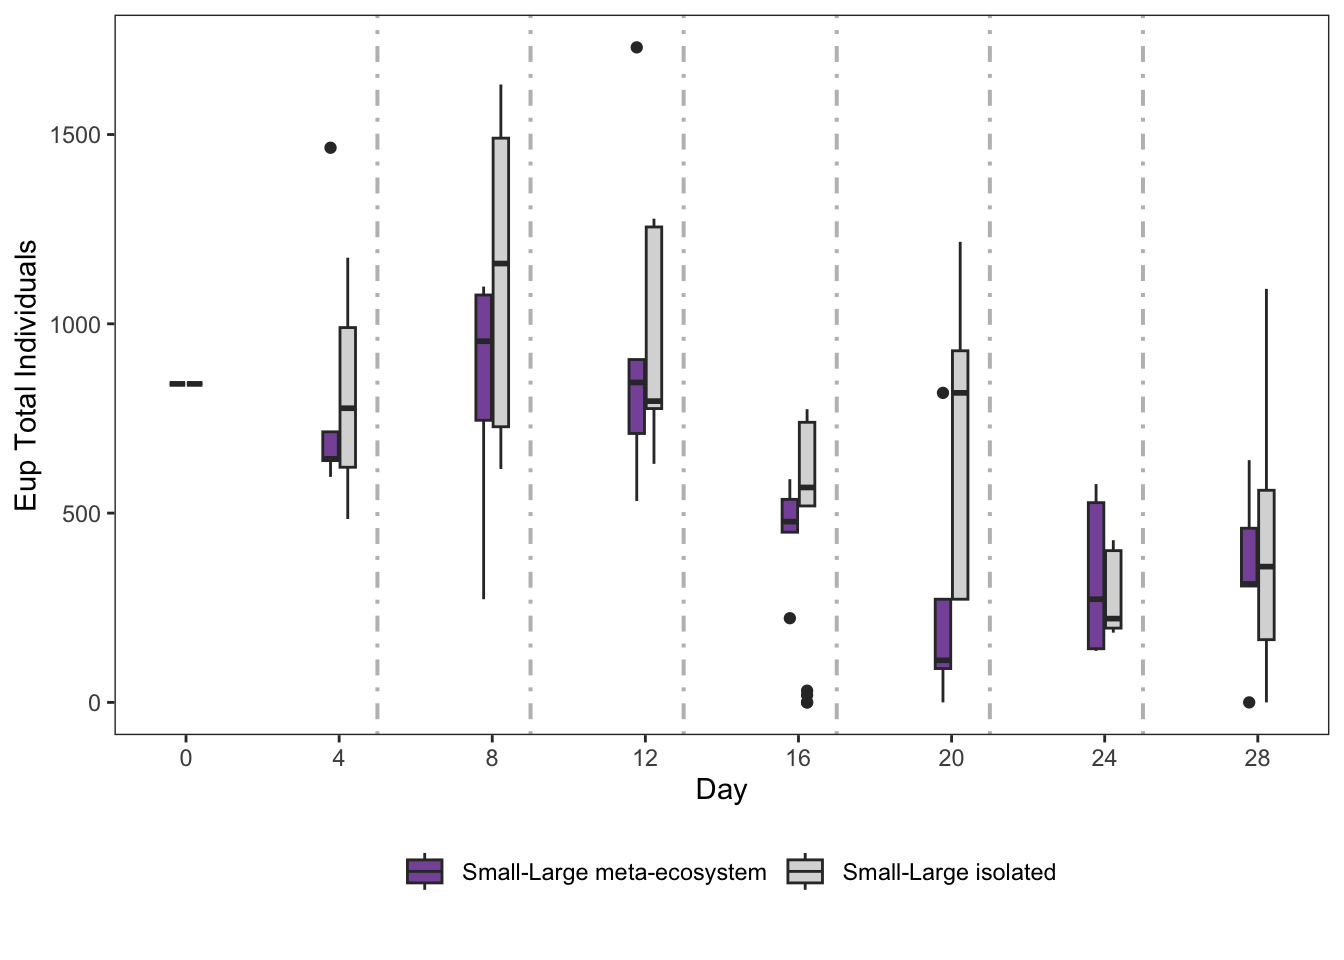
\includegraphics{index_files/figure-latex/unnamed-chunk-140-1.pdf}

\hypertarget{boxplots}{%
\subparagraph{Boxplots}\label{boxplots}}

\begin{Shaded}
\begin{Highlighting}[]
\FunctionTok{plot.metaecos.boxplots}\NormalTok{(ds\_metaecosystems, metaecosystem\_type\_input,}
\NormalTok{                       response\_variable)}
\end{Highlighting}
\end{Shaded}

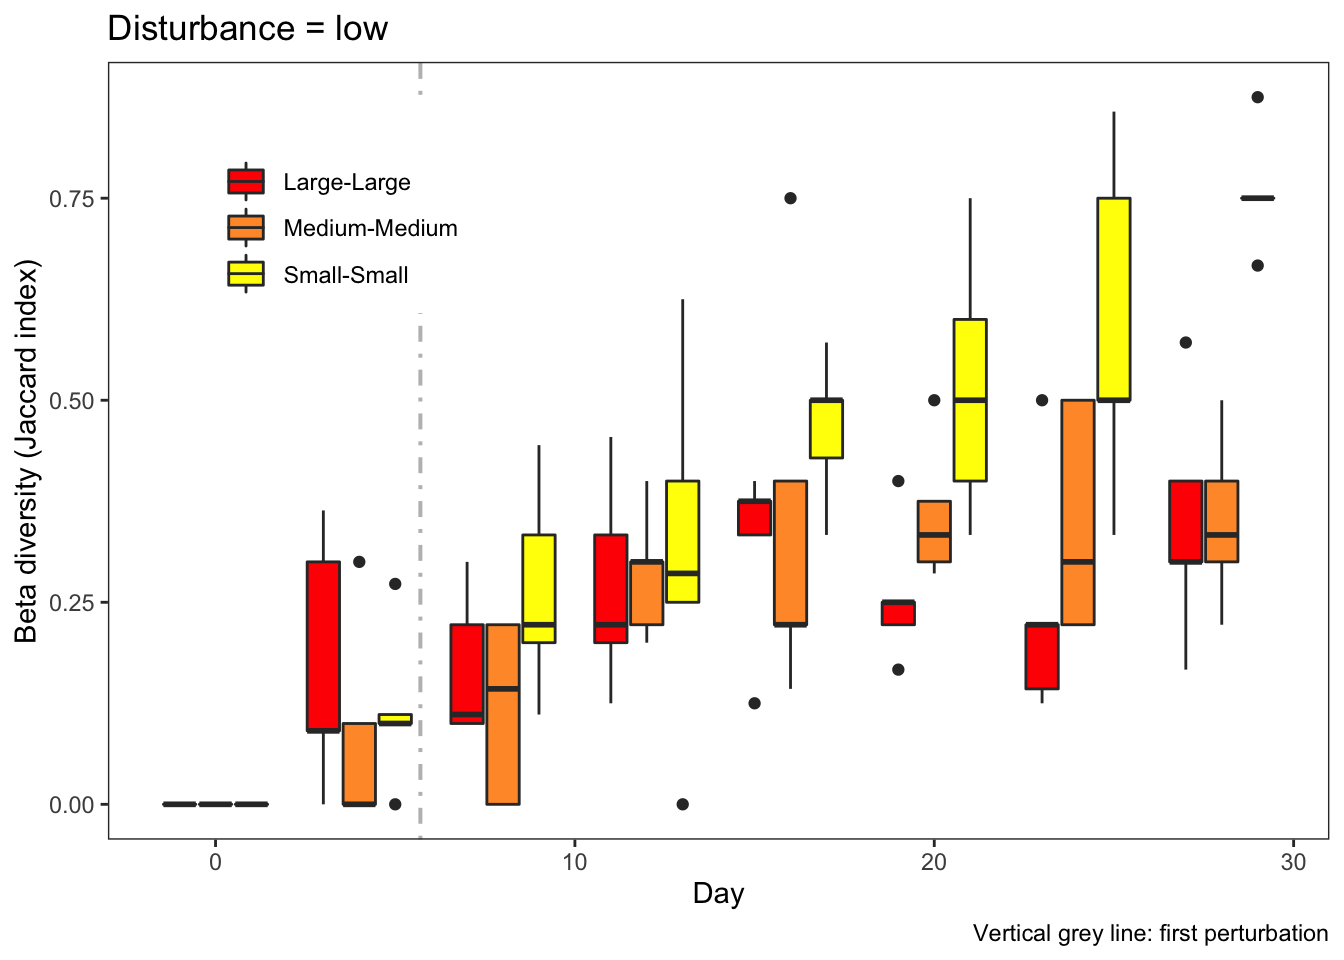
\includegraphics{index_files/figure-latex/unnamed-chunk-141-1.pdf}

\hypertarget{shannon}{%
\paragraph{Shannon}\label{shannon}}

\begin{Shaded}
\begin{Highlighting}[]
\NormalTok{response\_variable }\OtherTok{=} \StringTok{"mean\_shannon"}
\end{Highlighting}
\end{Shaded}

\hypertarget{means-1}{%
\subparagraph{Means}\label{means-1}}

\begin{Shaded}
\begin{Highlighting}[]
\FunctionTok{plot.metaecos.points}\NormalTok{(ds\_metaecosystems, metaecosystem\_type\_input,}
\NormalTok{                     response\_variable)}
\end{Highlighting}
\end{Shaded}

\begin{verbatim}
## Warning in grid.Call(C_textBounds, as.graphicsAnnot(x$label), x$x, x$y, :
## conversion failure on 'α Diversity' in 'mbcsToSbcs': dot substituted for <ce>
\end{verbatim}

\begin{verbatim}
## Warning in grid.Call(C_textBounds, as.graphicsAnnot(x$label), x$x, x$y, :
## conversion failure on 'α Diversity' in 'mbcsToSbcs': dot substituted for <b1>
\end{verbatim}

\begin{verbatim}
## Warning in grid.Call(C_textBounds, as.graphicsAnnot(x$label), x$x, x$y, :
## conversion failure on 'α Diversity' in 'mbcsToSbcs': dot substituted for <ce>
\end{verbatim}

\begin{verbatim}
## Warning in grid.Call(C_textBounds, as.graphicsAnnot(x$label), x$x, x$y, :
## conversion failure on 'α Diversity' in 'mbcsToSbcs': dot substituted for <b1>
\end{verbatim}

\begin{verbatim}
## Warning in grid.Call(C_textBounds, as.graphicsAnnot(x$label), x$x, x$y, :
## conversion failure on 'α Diversity' in 'mbcsToSbcs': dot substituted for <ce>
\end{verbatim}

\begin{verbatim}
## Warning in grid.Call(C_textBounds, as.graphicsAnnot(x$label), x$x, x$y, :
## conversion failure on 'α Diversity' in 'mbcsToSbcs': dot substituted for <b1>
\end{verbatim}

\begin{verbatim}
## Warning in grid.Call(C_textBounds, as.graphicsAnnot(x$label), x$x, x$y, :
## conversion failure on 'α Diversity' in 'mbcsToSbcs': dot substituted for <ce>
\end{verbatim}

\begin{verbatim}
## Warning in grid.Call(C_textBounds, as.graphicsAnnot(x$label), x$x, x$y, :
## conversion failure on 'α Diversity' in 'mbcsToSbcs': dot substituted for <b1>
\end{verbatim}

\begin{verbatim}
## Warning in grid.Call(C_textBounds, as.graphicsAnnot(x$label), x$x, x$y, :
## conversion failure on 'α Diversity' in 'mbcsToSbcs': dot substituted for <ce>
\end{verbatim}

\begin{verbatim}
## Warning in grid.Call(C_textBounds, as.graphicsAnnot(x$label), x$x, x$y, :
## conversion failure on 'α Diversity' in 'mbcsToSbcs': dot substituted for <b1>
\end{verbatim}

\begin{verbatim}
## Warning in grid.Call(C_textBounds, as.graphicsAnnot(x$label), x$x, x$y, :
## conversion failure on 'α Diversity' in 'mbcsToSbcs': dot substituted for <ce>
\end{verbatim}

\begin{verbatim}
## Warning in grid.Call(C_textBounds, as.graphicsAnnot(x$label), x$x, x$y, :
## conversion failure on 'α Diversity' in 'mbcsToSbcs': dot substituted for <b1>
\end{verbatim}

\begin{verbatim}
## Warning in grid.Call(C_textBounds, as.graphicsAnnot(x$label), x$x, x$y, :
## conversion failure on 'α Diversity' in 'mbcsToSbcs': dot substituted for <ce>
\end{verbatim}

\begin{verbatim}
## Warning in grid.Call(C_textBounds, as.graphicsAnnot(x$label), x$x, x$y, :
## conversion failure on 'α Diversity' in 'mbcsToSbcs': dot substituted for <b1>
\end{verbatim}

\begin{verbatim}
## Warning in grid.Call.graphics(C_text, as.graphicsAnnot(x$label), x$x, x$y, :
## conversion failure on 'α Diversity' in 'mbcsToSbcs': dot substituted for <ce>
\end{verbatim}

\begin{verbatim}
## Warning in grid.Call.graphics(C_text, as.graphicsAnnot(x$label), x$x, x$y, :
## conversion failure on 'α Diversity' in 'mbcsToSbcs': dot substituted for <b1>
\end{verbatim}

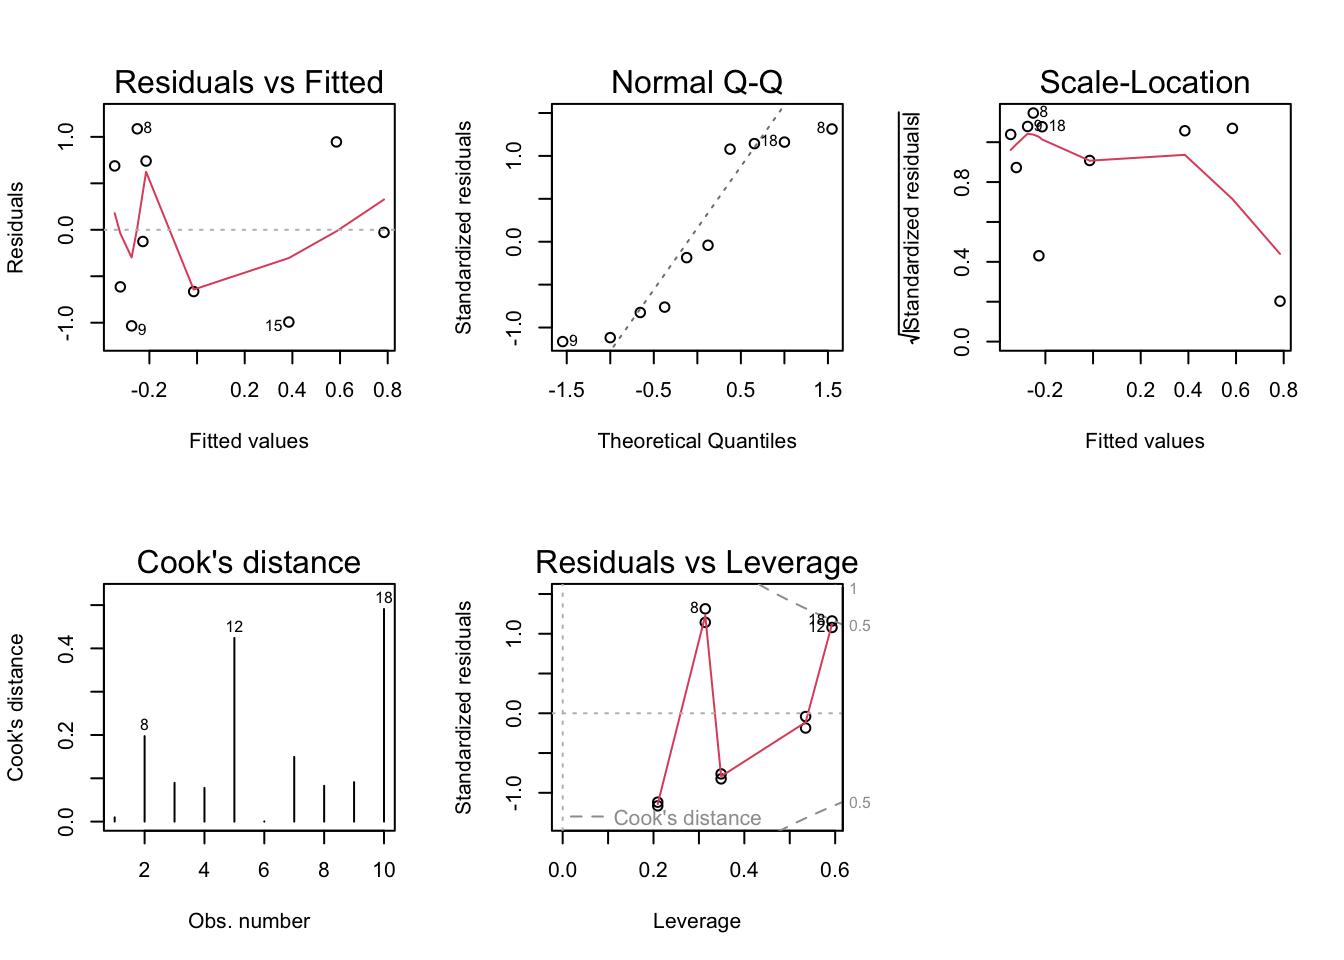
\includegraphics{index_files/figure-latex/unnamed-chunk-143-1.pdf}

\hypertarget{boxplots-1}{%
\subparagraph{Boxplots}\label{boxplots-1}}

\begin{Shaded}
\begin{Highlighting}[]
\FunctionTok{plot.metaecos.boxplots}\NormalTok{(ds\_metaecosystems, metaecosystem\_type\_input,}
\NormalTok{                       response\_variable)}
\end{Highlighting}
\end{Shaded}

\begin{verbatim}
## Warning in grid.Call(C_textBounds, as.graphicsAnnot(x$label), x$x, x$y, :
## conversion failure on 'α Diversity' in 'mbcsToSbcs': dot substituted for <ce>
\end{verbatim}

\begin{verbatim}
## Warning in grid.Call(C_textBounds, as.graphicsAnnot(x$label), x$x, x$y, :
## conversion failure on 'α Diversity' in 'mbcsToSbcs': dot substituted for <b1>
\end{verbatim}

\begin{verbatim}
## Warning in grid.Call(C_textBounds, as.graphicsAnnot(x$label), x$x, x$y, :
## conversion failure on 'α Diversity' in 'mbcsToSbcs': dot substituted for <ce>
\end{verbatim}

\begin{verbatim}
## Warning in grid.Call(C_textBounds, as.graphicsAnnot(x$label), x$x, x$y, :
## conversion failure on 'α Diversity' in 'mbcsToSbcs': dot substituted for <b1>
\end{verbatim}

\begin{verbatim}
## Warning in grid.Call(C_textBounds, as.graphicsAnnot(x$label), x$x, x$y, :
## conversion failure on 'α Diversity' in 'mbcsToSbcs': dot substituted for <ce>
\end{verbatim}

\begin{verbatim}
## Warning in grid.Call(C_textBounds, as.graphicsAnnot(x$label), x$x, x$y, :
## conversion failure on 'α Diversity' in 'mbcsToSbcs': dot substituted for <b1>
\end{verbatim}

\begin{verbatim}
## Warning in grid.Call(C_textBounds, as.graphicsAnnot(x$label), x$x, x$y, :
## conversion failure on 'α Diversity' in 'mbcsToSbcs': dot substituted for <ce>
\end{verbatim}

\begin{verbatim}
## Warning in grid.Call(C_textBounds, as.graphicsAnnot(x$label), x$x, x$y, :
## conversion failure on 'α Diversity' in 'mbcsToSbcs': dot substituted for <b1>
\end{verbatim}

\begin{verbatim}
## Warning in grid.Call(C_textBounds, as.graphicsAnnot(x$label), x$x, x$y, :
## conversion failure on 'α Diversity' in 'mbcsToSbcs': dot substituted for <ce>
\end{verbatim}

\begin{verbatim}
## Warning in grid.Call(C_textBounds, as.graphicsAnnot(x$label), x$x, x$y, :
## conversion failure on 'α Diversity' in 'mbcsToSbcs': dot substituted for <b1>
\end{verbatim}

\begin{verbatim}
## Warning in grid.Call(C_textBounds, as.graphicsAnnot(x$label), x$x, x$y, :
## conversion failure on 'α Diversity' in 'mbcsToSbcs': dot substituted for <ce>
\end{verbatim}

\begin{verbatim}
## Warning in grid.Call(C_textBounds, as.graphicsAnnot(x$label), x$x, x$y, :
## conversion failure on 'α Diversity' in 'mbcsToSbcs': dot substituted for <b1>
\end{verbatim}

\begin{verbatim}
## Warning in grid.Call(C_textBounds, as.graphicsAnnot(x$label), x$x, x$y, :
## conversion failure on 'α Diversity' in 'mbcsToSbcs': dot substituted for <ce>
\end{verbatim}

\begin{verbatim}
## Warning in grid.Call(C_textBounds, as.graphicsAnnot(x$label), x$x, x$y, :
## conversion failure on 'α Diversity' in 'mbcsToSbcs': dot substituted for <b1>
\end{verbatim}

\begin{verbatim}
## Warning in grid.Call.graphics(C_text, as.graphicsAnnot(x$label), x$x, x$y, :
## conversion failure on 'α Diversity' in 'mbcsToSbcs': dot substituted for <ce>
\end{verbatim}

\begin{verbatim}
## Warning in grid.Call.graphics(C_text, as.graphicsAnnot(x$label), x$x, x$y, :
## conversion failure on 'α Diversity' in 'mbcsToSbcs': dot substituted for <b1>
\end{verbatim}

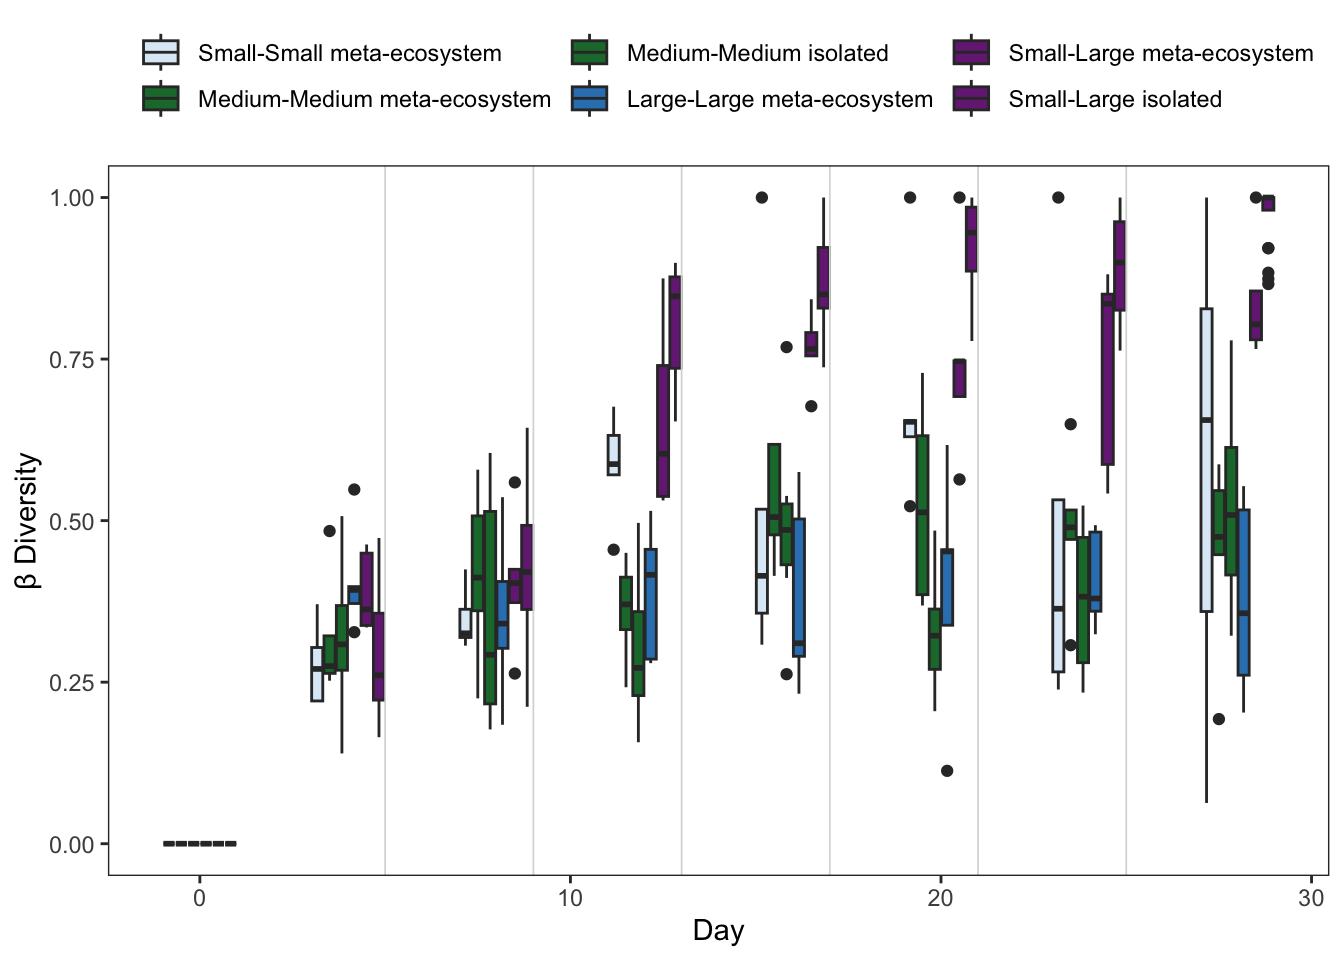
\includegraphics{index_files/figure-latex/unnamed-chunk-144-1.pdf}

\hypertarget{beta-diversity}{%
\paragraph{Beta diversity}\label{beta-diversity}}

\begin{Shaded}
\begin{Highlighting}[]
\NormalTok{response\_variable }\OtherTok{=} \StringTok{"bray\_curtis"}
\end{Highlighting}
\end{Shaded}

\hypertarget{means-2}{%
\subparagraph{Means}\label{means-2}}

\begin{Shaded}
\begin{Highlighting}[]
\FunctionTok{plot.metaecos.points}\NormalTok{(ds\_metaecosystems, metaecosystem\_type\_input,}
\NormalTok{                     response\_variable)}
\end{Highlighting}
\end{Shaded}

\begin{verbatim}
## Warning in grid.Call(C_textBounds, as.graphicsAnnot(x$label), x$x, x$y, :
## conversion failure on 'β Diversity' in 'mbcsToSbcs': dot substituted for <ce>
\end{verbatim}

\begin{verbatim}
## Warning in grid.Call(C_textBounds, as.graphicsAnnot(x$label), x$x, x$y, :
## conversion failure on 'β Diversity' in 'mbcsToSbcs': dot substituted for <b2>
\end{verbatim}

\begin{verbatim}
## Warning in grid.Call(C_textBounds, as.graphicsAnnot(x$label), x$x, x$y, :
## conversion failure on 'β Diversity' in 'mbcsToSbcs': dot substituted for <ce>
\end{verbatim}

\begin{verbatim}
## Warning in grid.Call(C_textBounds, as.graphicsAnnot(x$label), x$x, x$y, :
## conversion failure on 'β Diversity' in 'mbcsToSbcs': dot substituted for <b2>
\end{verbatim}

\begin{verbatim}
## Warning in grid.Call(C_textBounds, as.graphicsAnnot(x$label), x$x, x$y, :
## conversion failure on 'β Diversity' in 'mbcsToSbcs': dot substituted for <ce>
\end{verbatim}

\begin{verbatim}
## Warning in grid.Call(C_textBounds, as.graphicsAnnot(x$label), x$x, x$y, :
## conversion failure on 'β Diversity' in 'mbcsToSbcs': dot substituted for <b2>
\end{verbatim}

\begin{verbatim}
## Warning in grid.Call(C_textBounds, as.graphicsAnnot(x$label), x$x, x$y, :
## conversion failure on 'β Diversity' in 'mbcsToSbcs': dot substituted for <ce>
\end{verbatim}

\begin{verbatim}
## Warning in grid.Call(C_textBounds, as.graphicsAnnot(x$label), x$x, x$y, :
## conversion failure on 'β Diversity' in 'mbcsToSbcs': dot substituted for <b2>
\end{verbatim}

\begin{verbatim}
## Warning in grid.Call(C_textBounds, as.graphicsAnnot(x$label), x$x, x$y, :
## conversion failure on 'β Diversity' in 'mbcsToSbcs': dot substituted for <ce>
\end{verbatim}

\begin{verbatim}
## Warning in grid.Call(C_textBounds, as.graphicsAnnot(x$label), x$x, x$y, :
## conversion failure on 'β Diversity' in 'mbcsToSbcs': dot substituted for <b2>
\end{verbatim}

\begin{verbatim}
## Warning in grid.Call(C_textBounds, as.graphicsAnnot(x$label), x$x, x$y, :
## conversion failure on 'β Diversity' in 'mbcsToSbcs': dot substituted for <ce>
\end{verbatim}

\begin{verbatim}
## Warning in grid.Call(C_textBounds, as.graphicsAnnot(x$label), x$x, x$y, :
## conversion failure on 'β Diversity' in 'mbcsToSbcs': dot substituted for <b2>
\end{verbatim}

\begin{verbatim}
## Warning in grid.Call(C_textBounds, as.graphicsAnnot(x$label), x$x, x$y, :
## conversion failure on 'β Diversity' in 'mbcsToSbcs': dot substituted for <ce>
\end{verbatim}

\begin{verbatim}
## Warning in grid.Call(C_textBounds, as.graphicsAnnot(x$label), x$x, x$y, :
## conversion failure on 'β Diversity' in 'mbcsToSbcs': dot substituted for <b2>
\end{verbatim}

\begin{verbatim}
## Warning in grid.Call.graphics(C_text, as.graphicsAnnot(x$label), x$x, x$y, :
## conversion failure on 'β Diversity' in 'mbcsToSbcs': dot substituted for <ce>
\end{verbatim}

\begin{verbatim}
## Warning in grid.Call.graphics(C_text, as.graphicsAnnot(x$label), x$x, x$y, :
## conversion failure on 'β Diversity' in 'mbcsToSbcs': dot substituted for <b2>
\end{verbatim}

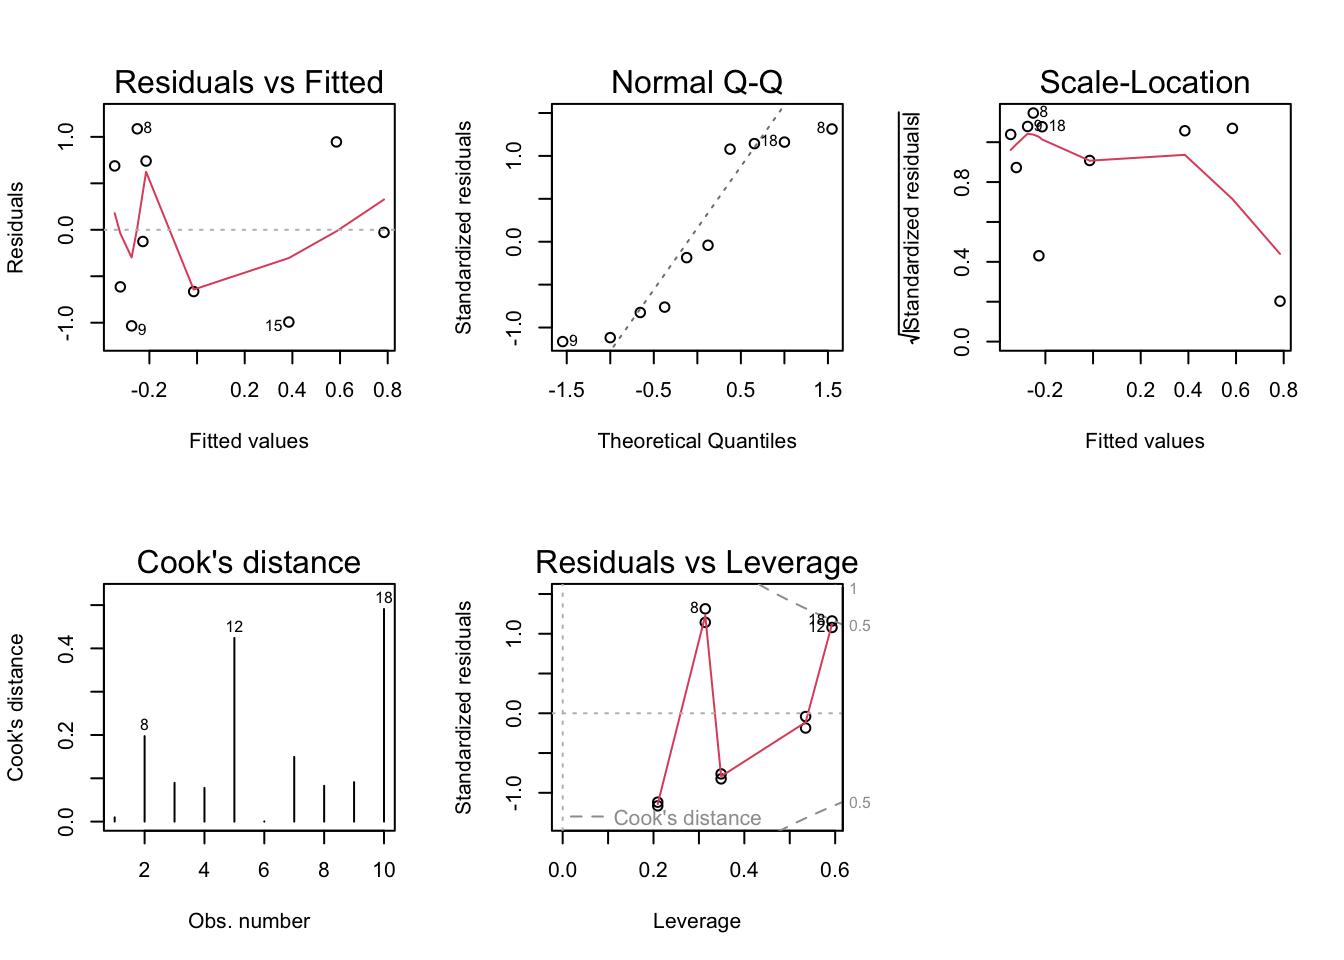
\includegraphics{index_files/figure-latex/unnamed-chunk-146-1.pdf}

\hypertarget{boxplots-2}{%
\subparagraph{Boxplots}\label{boxplots-2}}

\begin{Shaded}
\begin{Highlighting}[]
\FunctionTok{plot.metaecos.boxplots}\NormalTok{(ds\_metaecosystems, metaecosystem\_type\_input,}
\NormalTok{                       response\_variable)}
\end{Highlighting}
\end{Shaded}

\begin{verbatim}
## Warning in grid.Call(C_textBounds, as.graphicsAnnot(x$label), x$x, x$y, :
## conversion failure on 'β Diversity' in 'mbcsToSbcs': dot substituted for <ce>
\end{verbatim}

\begin{verbatim}
## Warning in grid.Call(C_textBounds, as.graphicsAnnot(x$label), x$x, x$y, :
## conversion failure on 'β Diversity' in 'mbcsToSbcs': dot substituted for <b2>
\end{verbatim}

\begin{verbatim}
## Warning in grid.Call(C_textBounds, as.graphicsAnnot(x$label), x$x, x$y, :
## conversion failure on 'β Diversity' in 'mbcsToSbcs': dot substituted for <ce>
\end{verbatim}

\begin{verbatim}
## Warning in grid.Call(C_textBounds, as.graphicsAnnot(x$label), x$x, x$y, :
## conversion failure on 'β Diversity' in 'mbcsToSbcs': dot substituted for <b2>
\end{verbatim}

\begin{verbatim}
## Warning in grid.Call(C_textBounds, as.graphicsAnnot(x$label), x$x, x$y, :
## conversion failure on 'β Diversity' in 'mbcsToSbcs': dot substituted for <ce>
\end{verbatim}

\begin{verbatim}
## Warning in grid.Call(C_textBounds, as.graphicsAnnot(x$label), x$x, x$y, :
## conversion failure on 'β Diversity' in 'mbcsToSbcs': dot substituted for <b2>
\end{verbatim}

\begin{verbatim}
## Warning in grid.Call(C_textBounds, as.graphicsAnnot(x$label), x$x, x$y, :
## conversion failure on 'β Diversity' in 'mbcsToSbcs': dot substituted for <ce>
\end{verbatim}

\begin{verbatim}
## Warning in grid.Call(C_textBounds, as.graphicsAnnot(x$label), x$x, x$y, :
## conversion failure on 'β Diversity' in 'mbcsToSbcs': dot substituted for <b2>
\end{verbatim}

\begin{verbatim}
## Warning in grid.Call(C_textBounds, as.graphicsAnnot(x$label), x$x, x$y, :
## conversion failure on 'β Diversity' in 'mbcsToSbcs': dot substituted for <ce>
\end{verbatim}

\begin{verbatim}
## Warning in grid.Call(C_textBounds, as.graphicsAnnot(x$label), x$x, x$y, :
## conversion failure on 'β Diversity' in 'mbcsToSbcs': dot substituted for <b2>
\end{verbatim}

\begin{verbatim}
## Warning in grid.Call(C_textBounds, as.graphicsAnnot(x$label), x$x, x$y, :
## conversion failure on 'β Diversity' in 'mbcsToSbcs': dot substituted for <ce>
\end{verbatim}

\begin{verbatim}
## Warning in grid.Call(C_textBounds, as.graphicsAnnot(x$label), x$x, x$y, :
## conversion failure on 'β Diversity' in 'mbcsToSbcs': dot substituted for <b2>
\end{verbatim}

\begin{verbatim}
## Warning in grid.Call(C_textBounds, as.graphicsAnnot(x$label), x$x, x$y, :
## conversion failure on 'β Diversity' in 'mbcsToSbcs': dot substituted for <ce>
\end{verbatim}

\begin{verbatim}
## Warning in grid.Call(C_textBounds, as.graphicsAnnot(x$label), x$x, x$y, :
## conversion failure on 'β Diversity' in 'mbcsToSbcs': dot substituted for <b2>
\end{verbatim}

\begin{verbatim}
## Warning in grid.Call.graphics(C_text, as.graphicsAnnot(x$label), x$x, x$y, :
## conversion failure on 'β Diversity' in 'mbcsToSbcs': dot substituted for <ce>
\end{verbatim}

\begin{verbatim}
## Warning in grid.Call.graphics(C_text, as.graphicsAnnot(x$label), x$x, x$y, :
## conversion failure on 'β Diversity' in 'mbcsToSbcs': dot substituted for <b2>
\end{verbatim}

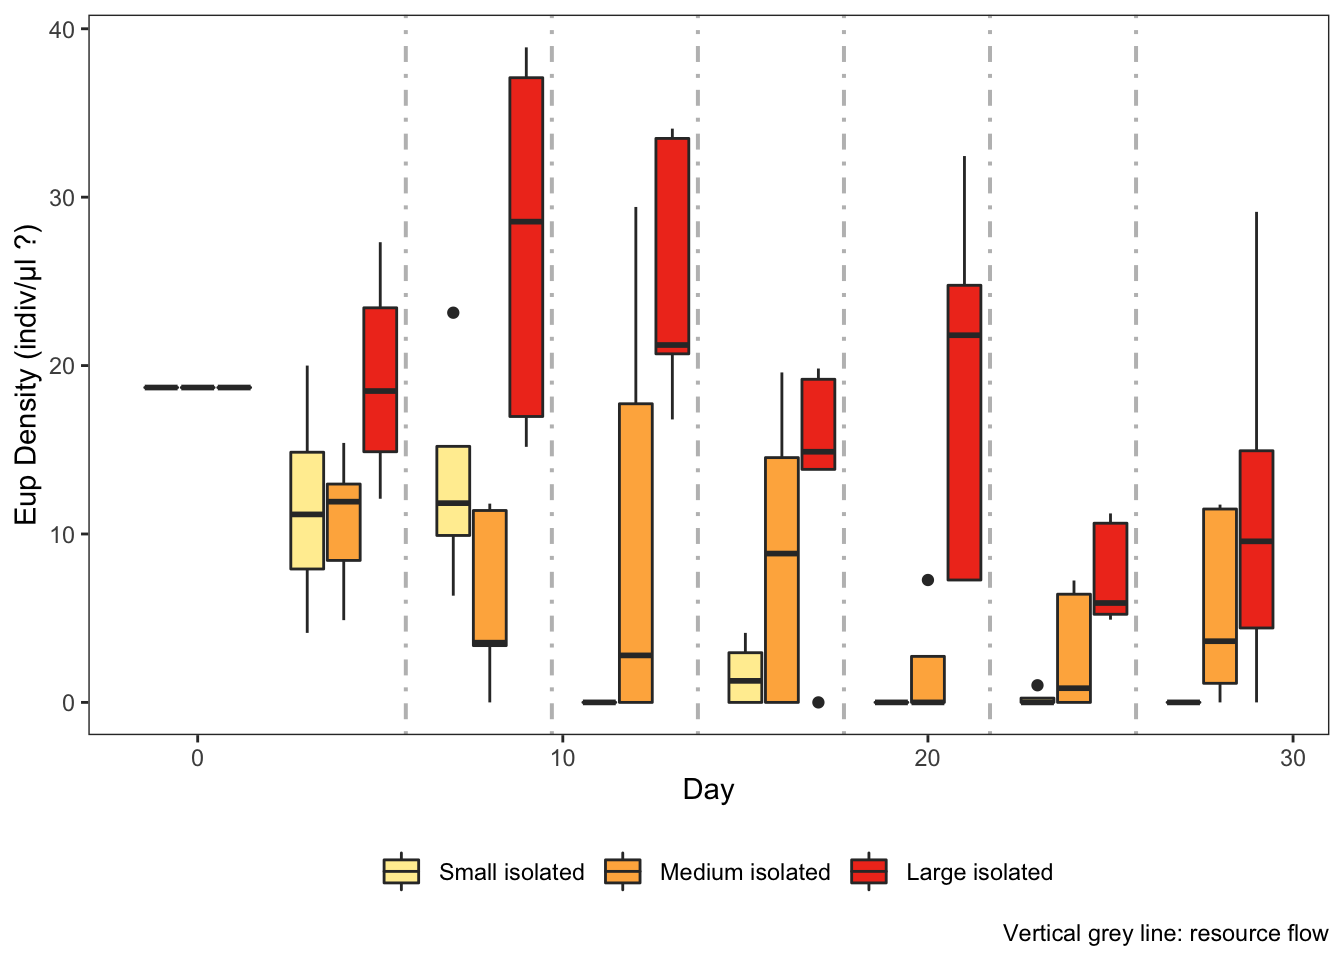
\includegraphics{index_files/figure-latex/unnamed-chunk-147-1.pdf}

\hypertarget{gamma-diversity}{%
\paragraph{Gamma diversity}\label{gamma-diversity}}

\begin{Shaded}
\begin{Highlighting}[]
\NormalTok{response\_variable }\OtherTok{=} \StringTok{"metaecosystem\_richness"}
\end{Highlighting}
\end{Shaded}

\hypertarget{means-3}{%
\subparagraph{Means}\label{means-3}}

\begin{Shaded}
\begin{Highlighting}[]
\FunctionTok{plot.metaecos.points}\NormalTok{(ds\_metaecosystems, metaecosystem\_type\_input,}
\NormalTok{                     response\_variable)}
\end{Highlighting}
\end{Shaded}

\begin{verbatim}
## Warning in grid.Call(C_textBounds, as.graphicsAnnot(x$label), x$x, x$y, :
## conversion failure on 'γ Diversity' in 'mbcsToSbcs': dot substituted for <ce>
\end{verbatim}

\begin{verbatim}
## Warning in grid.Call(C_textBounds, as.graphicsAnnot(x$label), x$x, x$y, :
## conversion failure on 'γ Diversity' in 'mbcsToSbcs': dot substituted for <b3>
\end{verbatim}

\begin{verbatim}
## Warning in grid.Call(C_textBounds, as.graphicsAnnot(x$label), x$x, x$y, :
## conversion failure on 'γ Diversity' in 'mbcsToSbcs': dot substituted for <ce>
\end{verbatim}

\begin{verbatim}
## Warning in grid.Call(C_textBounds, as.graphicsAnnot(x$label), x$x, x$y, :
## conversion failure on 'γ Diversity' in 'mbcsToSbcs': dot substituted for <b3>
\end{verbatim}

\begin{verbatim}
## Warning in grid.Call(C_textBounds, as.graphicsAnnot(x$label), x$x, x$y, :
## conversion failure on 'γ Diversity' in 'mbcsToSbcs': dot substituted for <ce>
\end{verbatim}

\begin{verbatim}
## Warning in grid.Call(C_textBounds, as.graphicsAnnot(x$label), x$x, x$y, :
## conversion failure on 'γ Diversity' in 'mbcsToSbcs': dot substituted for <b3>
\end{verbatim}

\begin{verbatim}
## Warning in grid.Call(C_textBounds, as.graphicsAnnot(x$label), x$x, x$y, :
## conversion failure on 'γ Diversity' in 'mbcsToSbcs': dot substituted for <ce>
\end{verbatim}

\begin{verbatim}
## Warning in grid.Call(C_textBounds, as.graphicsAnnot(x$label), x$x, x$y, :
## conversion failure on 'γ Diversity' in 'mbcsToSbcs': dot substituted for <b3>
\end{verbatim}

\begin{verbatim}
## Warning in grid.Call(C_textBounds, as.graphicsAnnot(x$label), x$x, x$y, :
## conversion failure on 'γ Diversity' in 'mbcsToSbcs': dot substituted for <ce>
\end{verbatim}

\begin{verbatim}
## Warning in grid.Call(C_textBounds, as.graphicsAnnot(x$label), x$x, x$y, :
## conversion failure on 'γ Diversity' in 'mbcsToSbcs': dot substituted for <b3>
\end{verbatim}

\begin{verbatim}
## Warning in grid.Call(C_textBounds, as.graphicsAnnot(x$label), x$x, x$y, :
## conversion failure on 'γ Diversity' in 'mbcsToSbcs': dot substituted for <ce>
\end{verbatim}

\begin{verbatim}
## Warning in grid.Call(C_textBounds, as.graphicsAnnot(x$label), x$x, x$y, :
## conversion failure on 'γ Diversity' in 'mbcsToSbcs': dot substituted for <b3>
\end{verbatim}

\begin{verbatim}
## Warning in grid.Call(C_textBounds, as.graphicsAnnot(x$label), x$x, x$y, :
## conversion failure on 'γ Diversity' in 'mbcsToSbcs': dot substituted for <ce>
\end{verbatim}

\begin{verbatim}
## Warning in grid.Call(C_textBounds, as.graphicsAnnot(x$label), x$x, x$y, :
## conversion failure on 'γ Diversity' in 'mbcsToSbcs': dot substituted for <b3>
\end{verbatim}

\begin{verbatim}
## Warning in grid.Call.graphics(C_text, as.graphicsAnnot(x$label), x$x, x$y, :
## conversion failure on 'γ Diversity' in 'mbcsToSbcs': dot substituted for <ce>
\end{verbatim}

\begin{verbatim}
## Warning in grid.Call.graphics(C_text, as.graphicsAnnot(x$label), x$x, x$y, :
## conversion failure on 'γ Diversity' in 'mbcsToSbcs': dot substituted for <b3>
\end{verbatim}

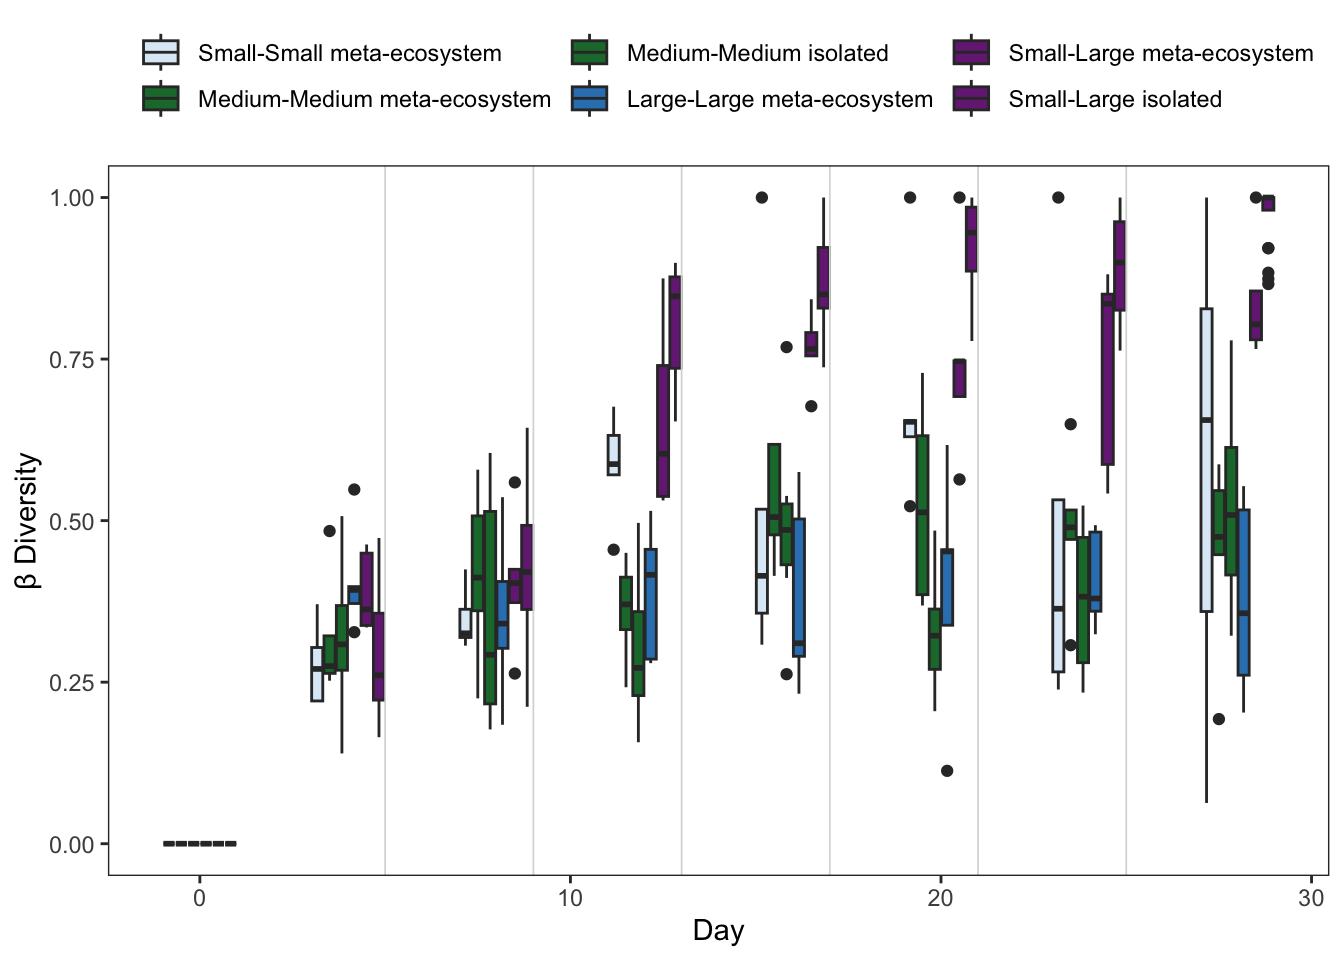
\includegraphics{index_files/figure-latex/unnamed-chunk-149-1.pdf}

\hypertarget{boxplots-3}{%
\subparagraph{Boxplots}\label{boxplots-3}}

\begin{Shaded}
\begin{Highlighting}[]
\FunctionTok{plot.metaecos.boxplots}\NormalTok{(ds\_metaecosystems, metaecosystem\_type\_input,}
\NormalTok{                       response\_variable)}
\end{Highlighting}
\end{Shaded}

\begin{verbatim}
## Warning in grid.Call(C_textBounds, as.graphicsAnnot(x$label), x$x, x$y, :
## conversion failure on 'γ Diversity' in 'mbcsToSbcs': dot substituted for <ce>
\end{verbatim}

\begin{verbatim}
## Warning in grid.Call(C_textBounds, as.graphicsAnnot(x$label), x$x, x$y, :
## conversion failure on 'γ Diversity' in 'mbcsToSbcs': dot substituted for <b3>
\end{verbatim}

\begin{verbatim}
## Warning in grid.Call(C_textBounds, as.graphicsAnnot(x$label), x$x, x$y, :
## conversion failure on 'γ Diversity' in 'mbcsToSbcs': dot substituted for <ce>
\end{verbatim}

\begin{verbatim}
## Warning in grid.Call(C_textBounds, as.graphicsAnnot(x$label), x$x, x$y, :
## conversion failure on 'γ Diversity' in 'mbcsToSbcs': dot substituted for <b3>
\end{verbatim}

\begin{verbatim}
## Warning in grid.Call(C_textBounds, as.graphicsAnnot(x$label), x$x, x$y, :
## conversion failure on 'γ Diversity' in 'mbcsToSbcs': dot substituted for <ce>
\end{verbatim}

\begin{verbatim}
## Warning in grid.Call(C_textBounds, as.graphicsAnnot(x$label), x$x, x$y, :
## conversion failure on 'γ Diversity' in 'mbcsToSbcs': dot substituted for <b3>
\end{verbatim}

\begin{verbatim}
## Warning in grid.Call(C_textBounds, as.graphicsAnnot(x$label), x$x, x$y, :
## conversion failure on 'γ Diversity' in 'mbcsToSbcs': dot substituted for <ce>
\end{verbatim}

\begin{verbatim}
## Warning in grid.Call(C_textBounds, as.graphicsAnnot(x$label), x$x, x$y, :
## conversion failure on 'γ Diversity' in 'mbcsToSbcs': dot substituted for <b3>
\end{verbatim}

\begin{verbatim}
## Warning in grid.Call(C_textBounds, as.graphicsAnnot(x$label), x$x, x$y, :
## conversion failure on 'γ Diversity' in 'mbcsToSbcs': dot substituted for <ce>
\end{verbatim}

\begin{verbatim}
## Warning in grid.Call(C_textBounds, as.graphicsAnnot(x$label), x$x, x$y, :
## conversion failure on 'γ Diversity' in 'mbcsToSbcs': dot substituted for <b3>
\end{verbatim}

\begin{verbatim}
## Warning in grid.Call(C_textBounds, as.graphicsAnnot(x$label), x$x, x$y, :
## conversion failure on 'γ Diversity' in 'mbcsToSbcs': dot substituted for <ce>
\end{verbatim}

\begin{verbatim}
## Warning in grid.Call(C_textBounds, as.graphicsAnnot(x$label), x$x, x$y, :
## conversion failure on 'γ Diversity' in 'mbcsToSbcs': dot substituted for <b3>
\end{verbatim}

\begin{verbatim}
## Warning in grid.Call(C_textBounds, as.graphicsAnnot(x$label), x$x, x$y, :
## conversion failure on 'γ Diversity' in 'mbcsToSbcs': dot substituted for <ce>
\end{verbatim}

\begin{verbatim}
## Warning in grid.Call(C_textBounds, as.graphicsAnnot(x$label), x$x, x$y, :
## conversion failure on 'γ Diversity' in 'mbcsToSbcs': dot substituted for <b3>
\end{verbatim}

\begin{verbatim}
## Warning in grid.Call.graphics(C_text, as.graphicsAnnot(x$label), x$x, x$y, :
## conversion failure on 'γ Diversity' in 'mbcsToSbcs': dot substituted for <ce>
\end{verbatim}

\begin{verbatim}
## Warning in grid.Call.graphics(C_text, as.graphicsAnnot(x$label), x$x, x$y, :
## conversion failure on 'γ Diversity' in 'mbcsToSbcs': dot substituted for <b3>
\end{verbatim}

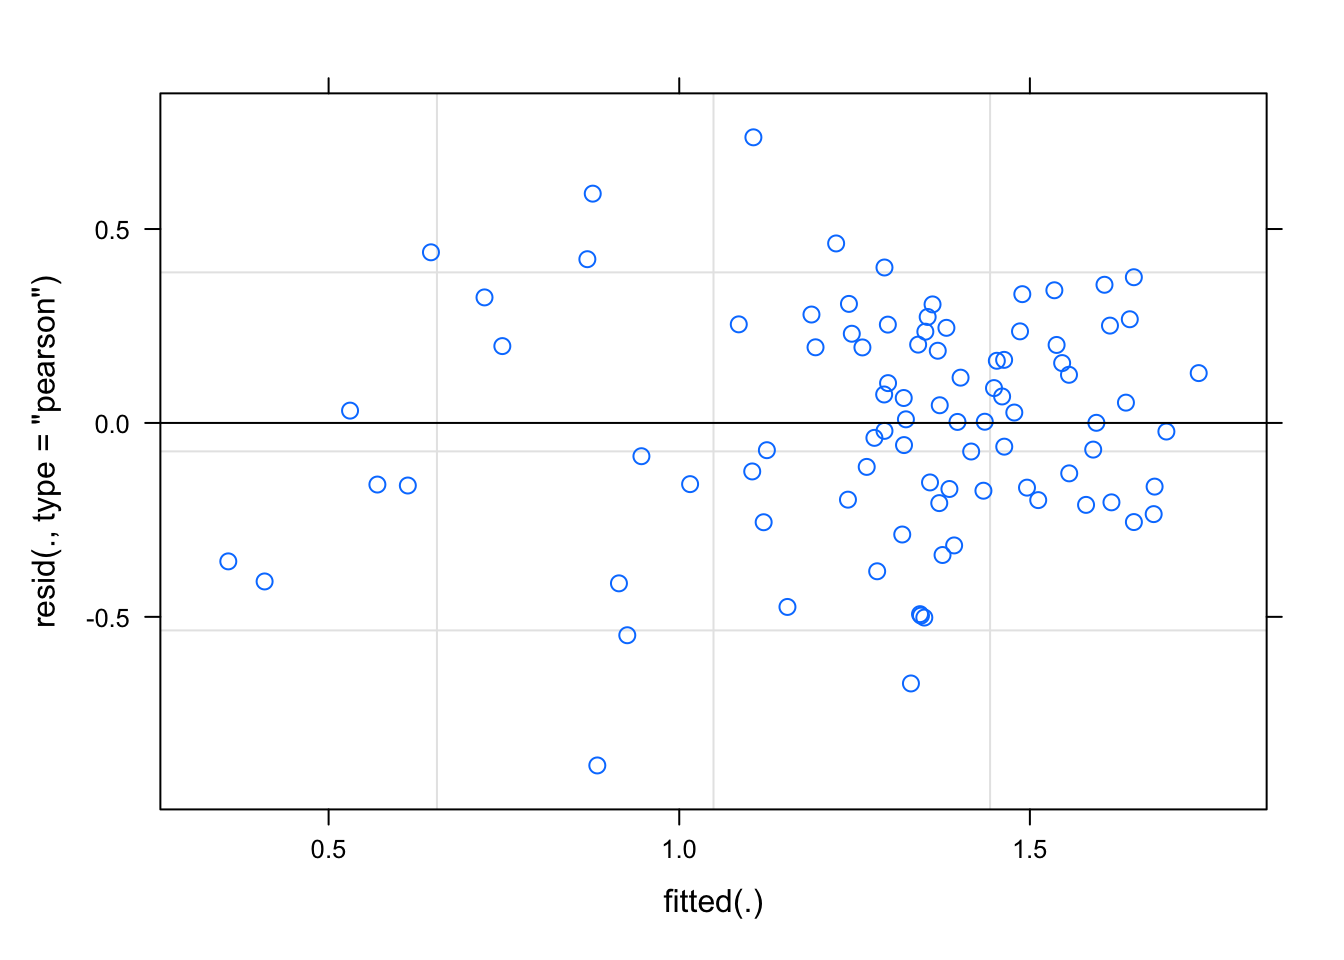
\includegraphics{index_files/figure-latex/unnamed-chunk-150-1.pdf}

\hypertarget{mm-vs-sl-meta-ecosystems-and-isolated}{%
\subsubsection{MM vs SL (meta-ecosystems and
isolated)}\label{mm-vs-sl-meta-ecosystems-and-isolated}}

\begin{Shaded}
\begin{Highlighting}[]
\NormalTok{metaecosystem\_type\_input }\OtherTok{=} \FunctionTok{c}\NormalTok{(}
  \StringTok{"Medium{-}Medium meta{-}ecosystem"}\NormalTok{,}
  \StringTok{"Medium{-}Medium isolated"}\NormalTok{,}
  \StringTok{"Small{-}Large meta{-}ecosystem"}\NormalTok{,}
  \StringTok{"Small{-}Large isolated"}
\NormalTok{)}
\end{Highlighting}
\end{Shaded}

\hypertarget{biomass-1}{%
\paragraph{Biomass}\label{biomass-1}}

\begin{Shaded}
\begin{Highlighting}[]
\NormalTok{response\_variable }\OtherTok{=} \StringTok{"total\_metaecosystem\_bioarea\_mm2"}
\end{Highlighting}
\end{Shaded}

\hypertarget{means-4}{%
\subparagraph{Means}\label{means-4}}

\begin{Shaded}
\begin{Highlighting}[]
\NormalTok{p\_MM\_SL\_metaecos\_biomass }\OtherTok{=} \FunctionTok{plot.metaecos.points}\NormalTok{(ds\_metaecosystems, }
\NormalTok{                                                metaecosystem\_type\_input,}
\NormalTok{                                                response\_variable) }\SpecialCharTok{\%\textgreater{}\%}
  \FunctionTok{print}\NormalTok{()}
\end{Highlighting}
\end{Shaded}

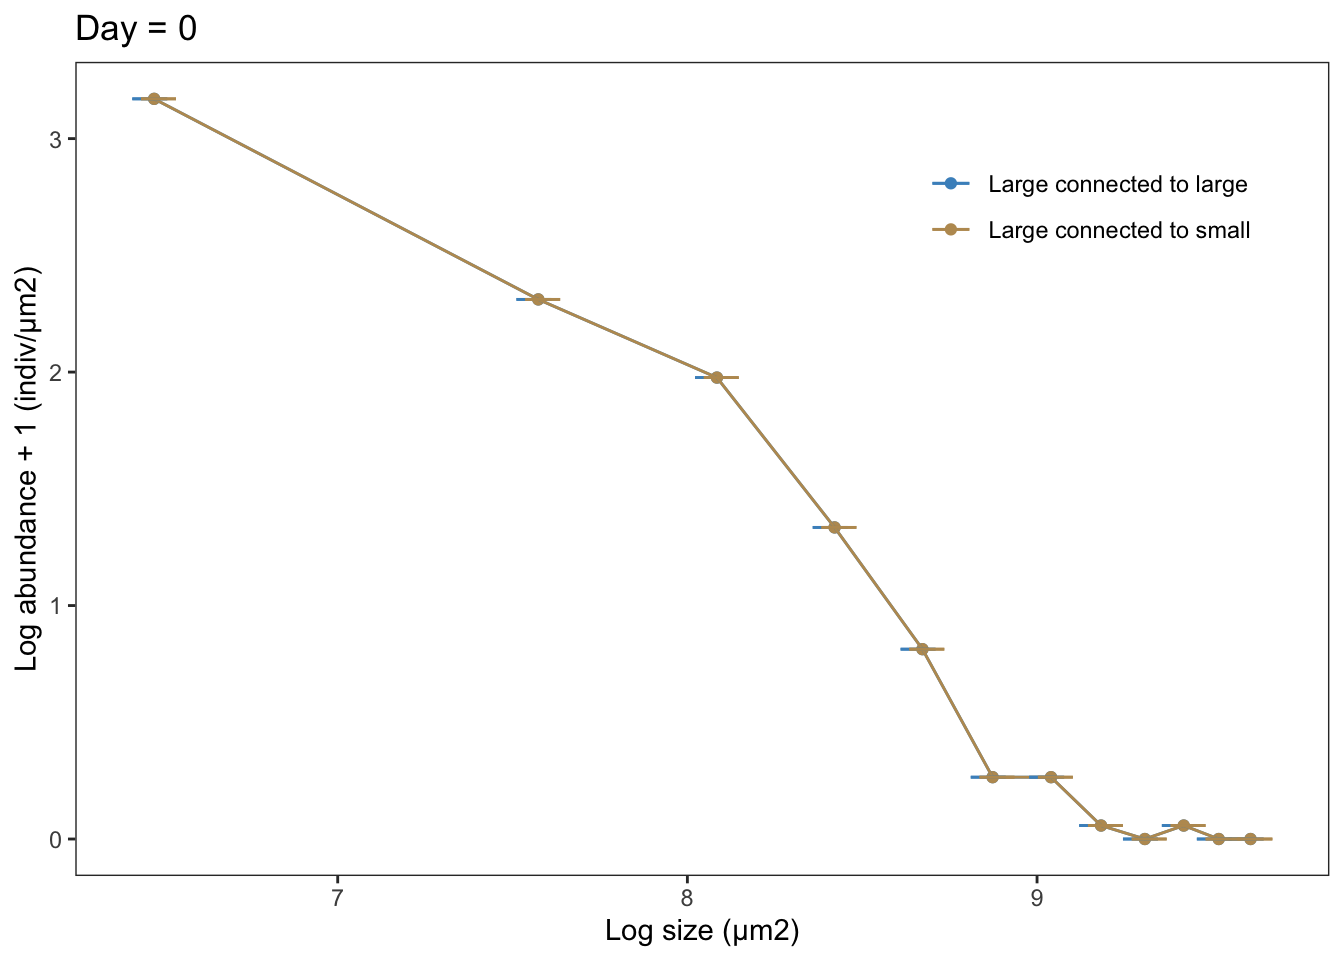
\includegraphics{index_files/figure-latex/unnamed-chunk-152-1.pdf}

Small-Large vs Medium-Medium meta-ecosystems

\begin{Shaded}
\begin{Highlighting}[]
\NormalTok{metaecosystem\_type\_input\_model }\OtherTok{=} \FunctionTok{c}\NormalTok{(}\StringTok{"Small{-}Large meta{-}ecosystem"}\NormalTok{,}
                                   \StringTok{"Medium{-}Medium meta{-}ecosystem"}\NormalTok{)}
\end{Highlighting}
\end{Shaded}

\begin{Shaded}
\begin{Highlighting}[]
\NormalTok{filtered\_data }\OtherTok{=}\NormalTok{ ds\_metaecosystems }\SpecialCharTok{\%\textgreater{}\%}
                         \FunctionTok{filter}\NormalTok{(time\_point }\SpecialCharTok{\textgreater{}=}\NormalTok{ first\_time\_point\_model,}
\NormalTok{                                time\_point }\SpecialCharTok{\textless{}=}\NormalTok{ last\_time\_point\_model,}
\NormalTok{                                metaecosystem\_type }\SpecialCharTok{\%in\%}\NormalTok{ metaecosystem\_type\_input\_model)}
\end{Highlighting}
\end{Shaded}

\begin{Shaded}
\begin{Highlighting}[]
\FunctionTok{plot.metaecos.points}\NormalTok{(filtered\_data,}
\NormalTok{                     metaecosystem\_type\_input\_model,}
\NormalTok{                     response\_variable)}
\end{Highlighting}
\end{Shaded}

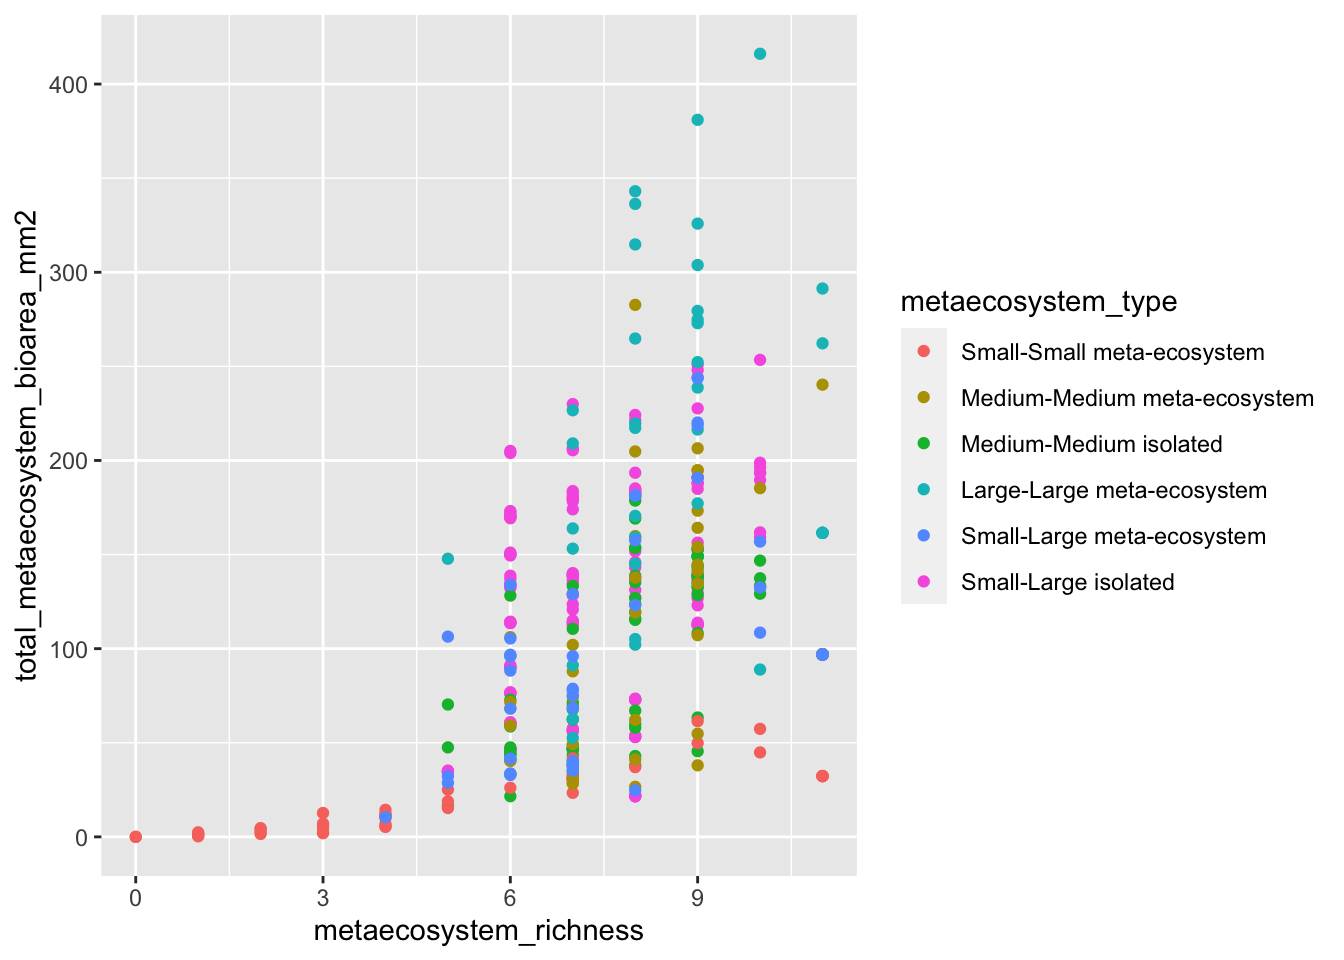
\includegraphics{index_files/figure-latex/unnamed-chunk-161-1.pdf}

\begin{itemize}
\tightlist
\item
  Null model
\end{itemize}

\begin{Shaded}
\begin{Highlighting}[]
\NormalTok{null\_model }\OtherTok{=} \FunctionTok{lmer}\NormalTok{(}
  \FunctionTok{get}\NormalTok{(response\_variable) }\SpecialCharTok{\textasciitilde{}}
\NormalTok{    day }\SpecialCharTok{+} 
\NormalTok{    (day }\SpecialCharTok{|}\NormalTok{ system\_nr), }
  \AttributeTok{data =}\NormalTok{ filtered\_data,}
  \AttributeTok{REML =} \ConstantTok{FALSE}\NormalTok{,}
  \AttributeTok{control =} \FunctionTok{lmerControl}\NormalTok{(}\AttributeTok{optimizer =} \StringTok{"Nelder\_Mead"}\NormalTok{)}
\NormalTok{)}

\FunctionTok{summary}\NormalTok{(null\_model)}
\end{Highlighting}
\end{Shaded}

\begin{verbatim}
## Linear mixed model fit by maximum likelihood  ['lmerMod']
## Formula: get(response_variable) ~ day + (day | system_nr)
##    Data: filtered_data
## Control: lmerControl(optimizer = "Nelder_Mead")
## 
##      AIC      BIC   logLik deviance df.resid 
##    598.5    611.1   -293.2    586.5       54 
## 
## Scaled residuals: 
##      Min       1Q   Median       3Q      Max 
## -3.06598 -0.39876  0.02834  0.55939  2.30337 
## 
## Random effects:
##  Groups    Name        Variance Std.Dev. Corr 
##  system_nr (Intercept) 1269.789 35.634        
##            day            1.603  1.266   -0.96
##  Residual               831.372 28.834        
## Number of obs: 60, groups:  system_nr, 10
## 
## Fixed effects:
##             Estimate Std. Error t value
## (Intercept) 256.7656    15.3960   16.68
## day          -7.4509     0.6762  -11.02
## 
## Correlation of Fixed Effects:
##     (Intr)
## day -0.929
\end{verbatim}

\begin{Shaded}
\begin{Highlighting}[]
\FunctionTok{plot}\NormalTok{(null\_model)}
\end{Highlighting}
\end{Shaded}

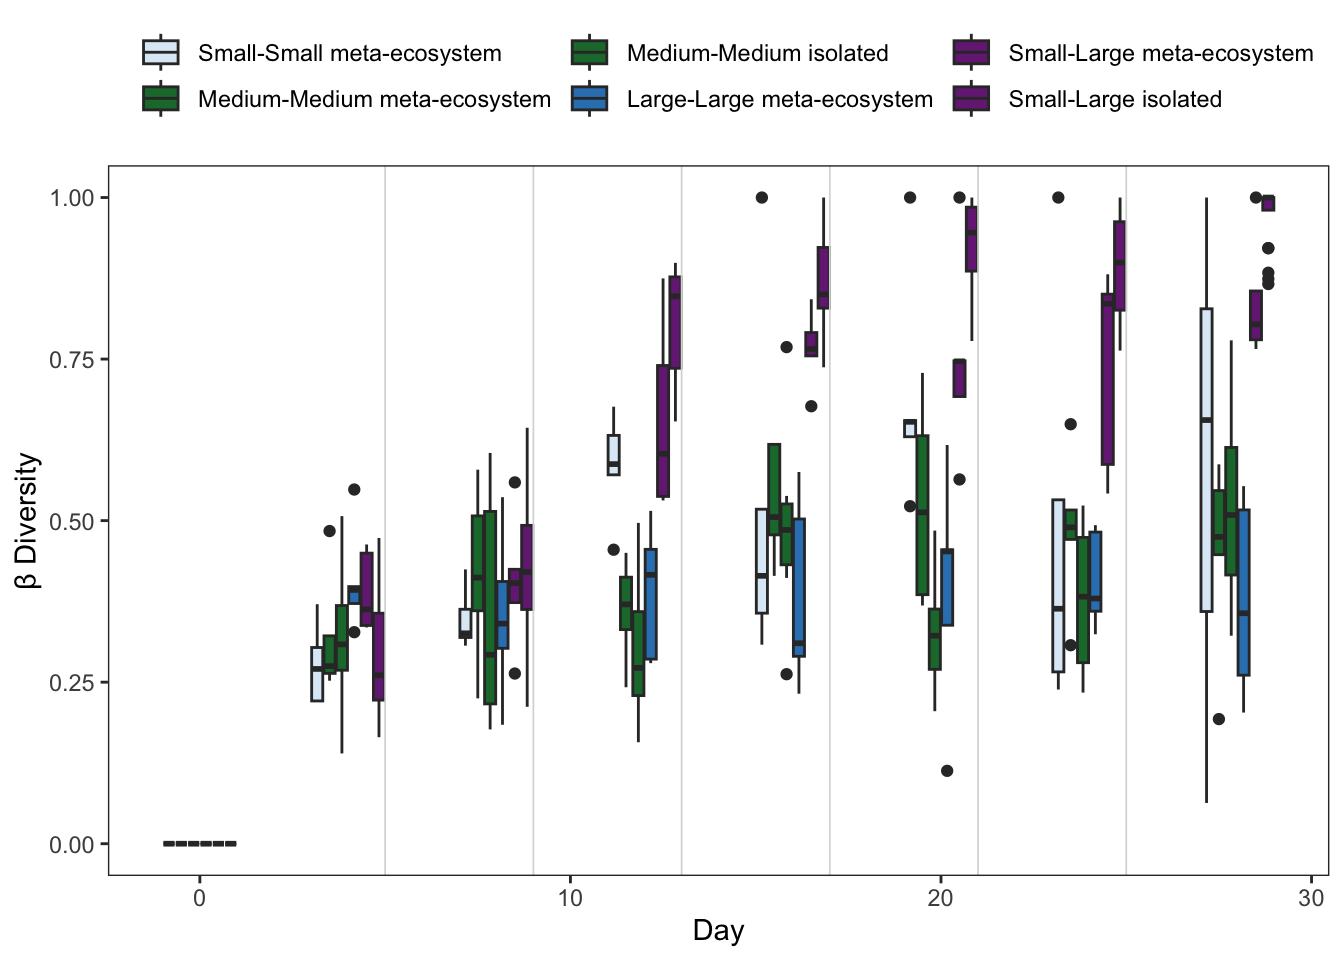
\includegraphics{index_files/figure-latex/unnamed-chunk-162-1.pdf}

\begin{Shaded}
\begin{Highlighting}[]
\FunctionTok{qqnorm}\NormalTok{(}\FunctionTok{resid}\NormalTok{(null\_model))}
\end{Highlighting}
\end{Shaded}

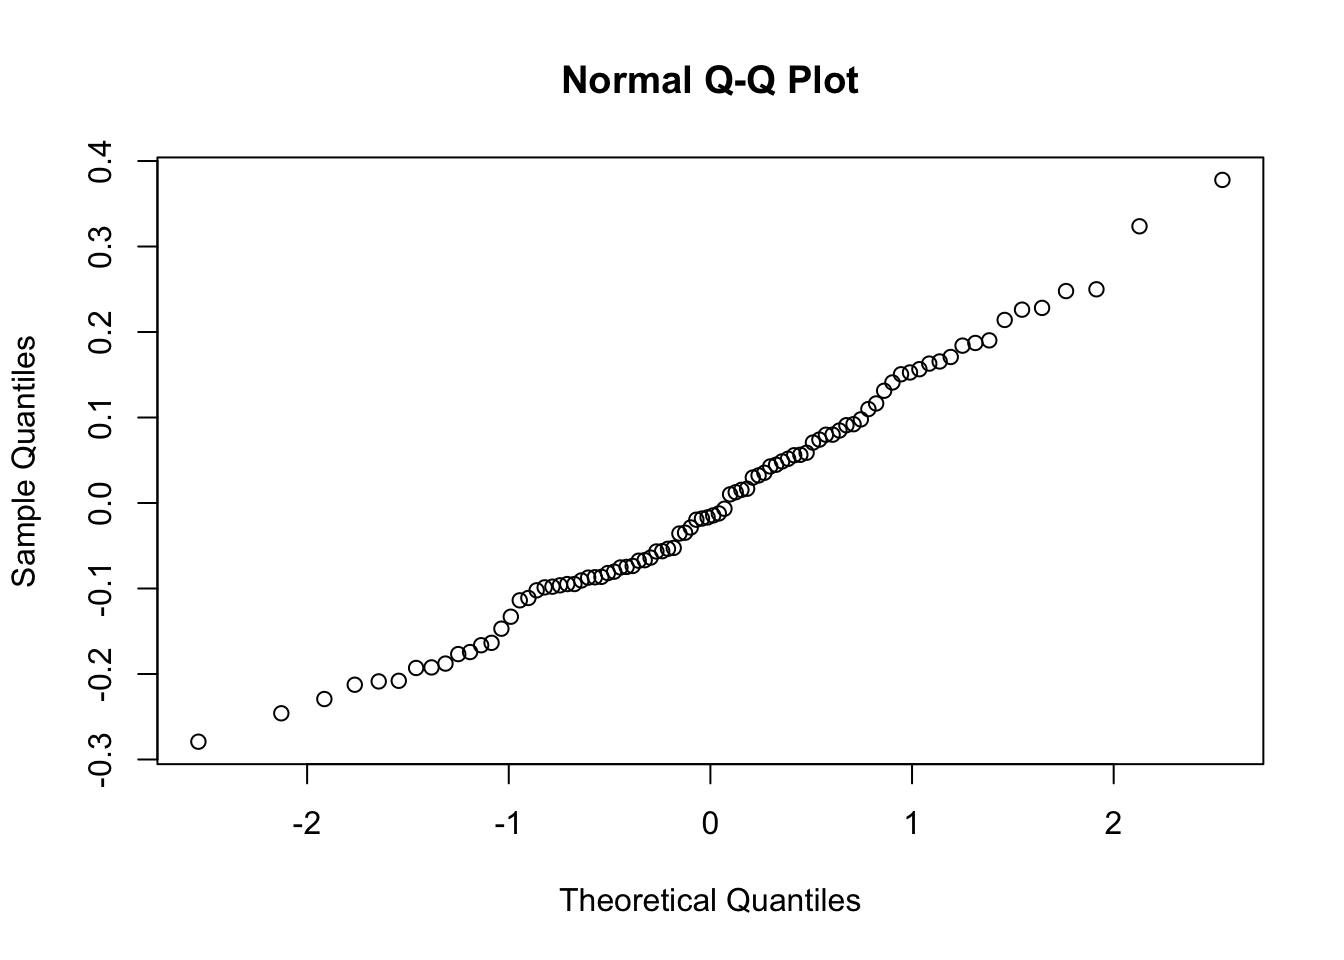
\includegraphics{index_files/figure-latex/unnamed-chunk-162-2.pdf}

\begin{itemize}
\tightlist
\item
  Full model (with \texttt{patch\_size\_symmetry} and
  \texttt{patch\_size\_symmetry:day})
\end{itemize}

\begin{Shaded}
\begin{Highlighting}[]
\NormalTok{full\_model }\OtherTok{=} \FunctionTok{lmer}\NormalTok{(}
  \FunctionTok{get}\NormalTok{(response\_variable) }\SpecialCharTok{\textasciitilde{}}
\NormalTok{    day }\SpecialCharTok{+} 
\NormalTok{    patch\_size\_symmetry }\SpecialCharTok{+}
\NormalTok{    patch\_size\_symmetry }\SpecialCharTok{:}\NormalTok{ day }\SpecialCharTok{+} 
\NormalTok{    (day }\SpecialCharTok{|}\NormalTok{ system\_nr), }
  \AttributeTok{data =}\NormalTok{ filtered\_data,}
  \AttributeTok{REML =} \ConstantTok{FALSE}\NormalTok{,}
  \AttributeTok{control =} \FunctionTok{lmerControl}\NormalTok{(}\AttributeTok{optimizer =} \StringTok{"Nelder\_Mead"}\NormalTok{)}
\NormalTok{)}

\FunctionTok{summary}\NormalTok{(full\_model)}
\end{Highlighting}
\end{Shaded}

\begin{verbatim}
## Linear mixed model fit by maximum likelihood  ['lmerMod']
## Formula: 
## get(response_variable) ~ day + patch_size_symmetry + patch_size_symmetry:day +  
##     (day | system_nr)
##    Data: filtered_data
## Control: lmerControl(optimizer = "Nelder_Mead")
## 
##      AIC      BIC   logLik deviance df.resid 
##    601.2    617.9   -292.6    585.2       52 
## 
## Scaled residuals: 
##      Min       1Q   Median       3Q      Max 
## -3.15415 -0.43689  0.04077  0.57459  2.17536 
## 
## Random effects:
##  Groups    Name        Variance Std.Dev. Corr 
##  system_nr (Intercept) 902.2492 30.0375       
##            day           0.8626  0.9288  -1.00
##  Residual              864.1128 29.3958       
## Number of obs: 60, groups:  system_nr, 10
## 
## Fixed effects:
##                                  Estimate Std. Error t value
## (Intercept)                      241.2323    20.2295  11.925
## day                               -6.9591     0.8887  -7.831
## patch_size_symmetrysymmetric      31.0667    28.6089   1.086
## day:patch_size_symmetrysymmetric  -0.9836     1.2568  -0.783
## 
## Correlation of Fixed Effects:
##             (Intr) day    ptch__
## day         -0.928              
## ptch_sz_sym -0.707  0.656       
## dy:ptch_sz_  0.656 -0.707 -0.928
## optimizer (Nelder_Mead) convergence code: 0 (OK)
## boundary (singular) fit: see help('isSingular')
\end{verbatim}

\begin{Shaded}
\begin{Highlighting}[]
\FunctionTok{plot}\NormalTok{(full\_model)}
\end{Highlighting}
\end{Shaded}

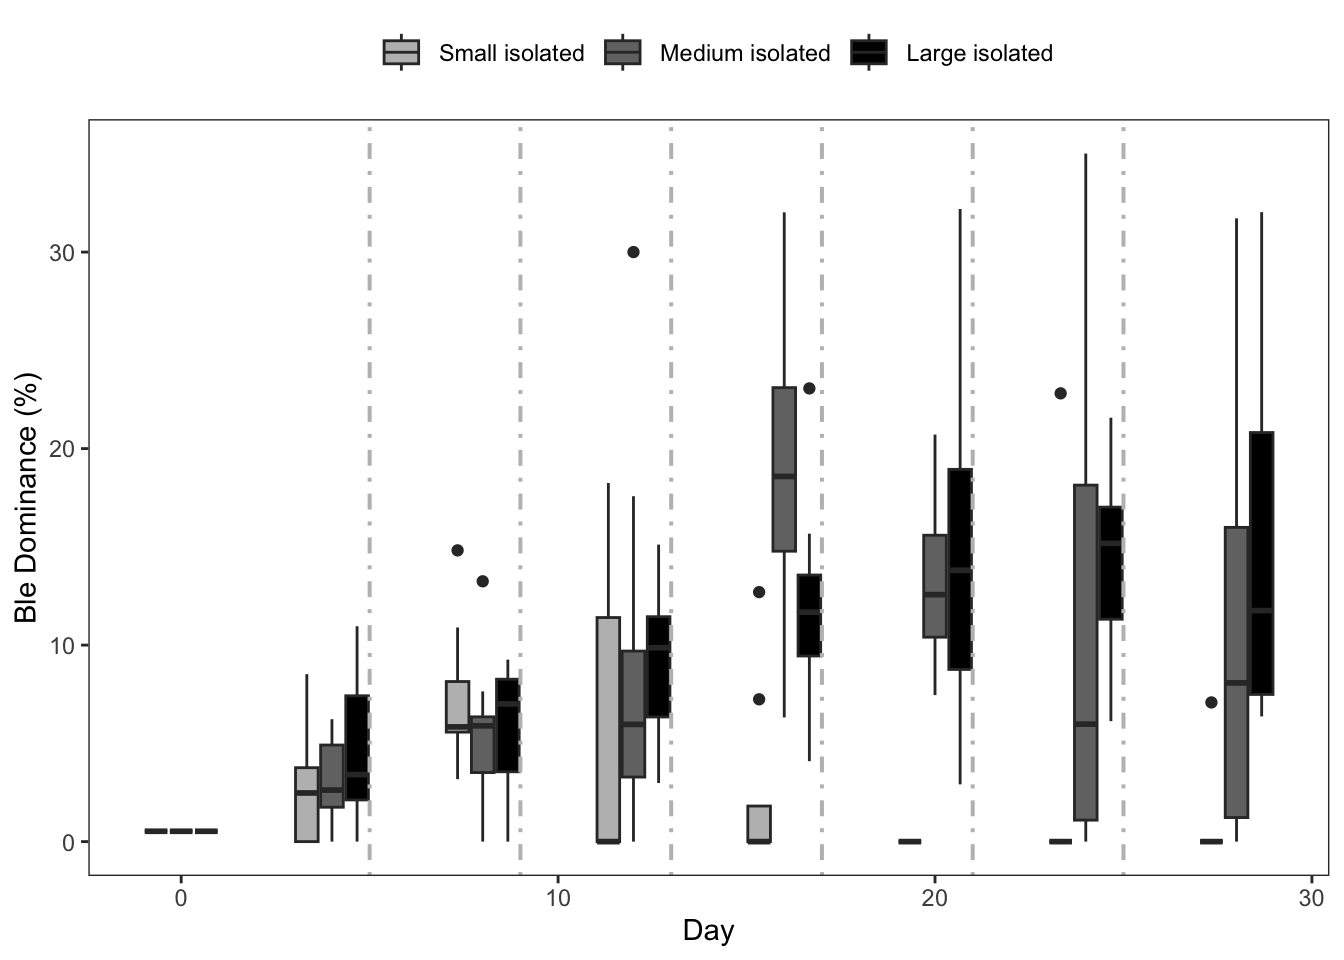
\includegraphics{index_files/figure-latex/unnamed-chunk-163-1.pdf}

\begin{Shaded}
\begin{Highlighting}[]
\FunctionTok{qqnorm}\NormalTok{(}\FunctionTok{resid}\NormalTok{(full\_model))}
\end{Highlighting}
\end{Shaded}

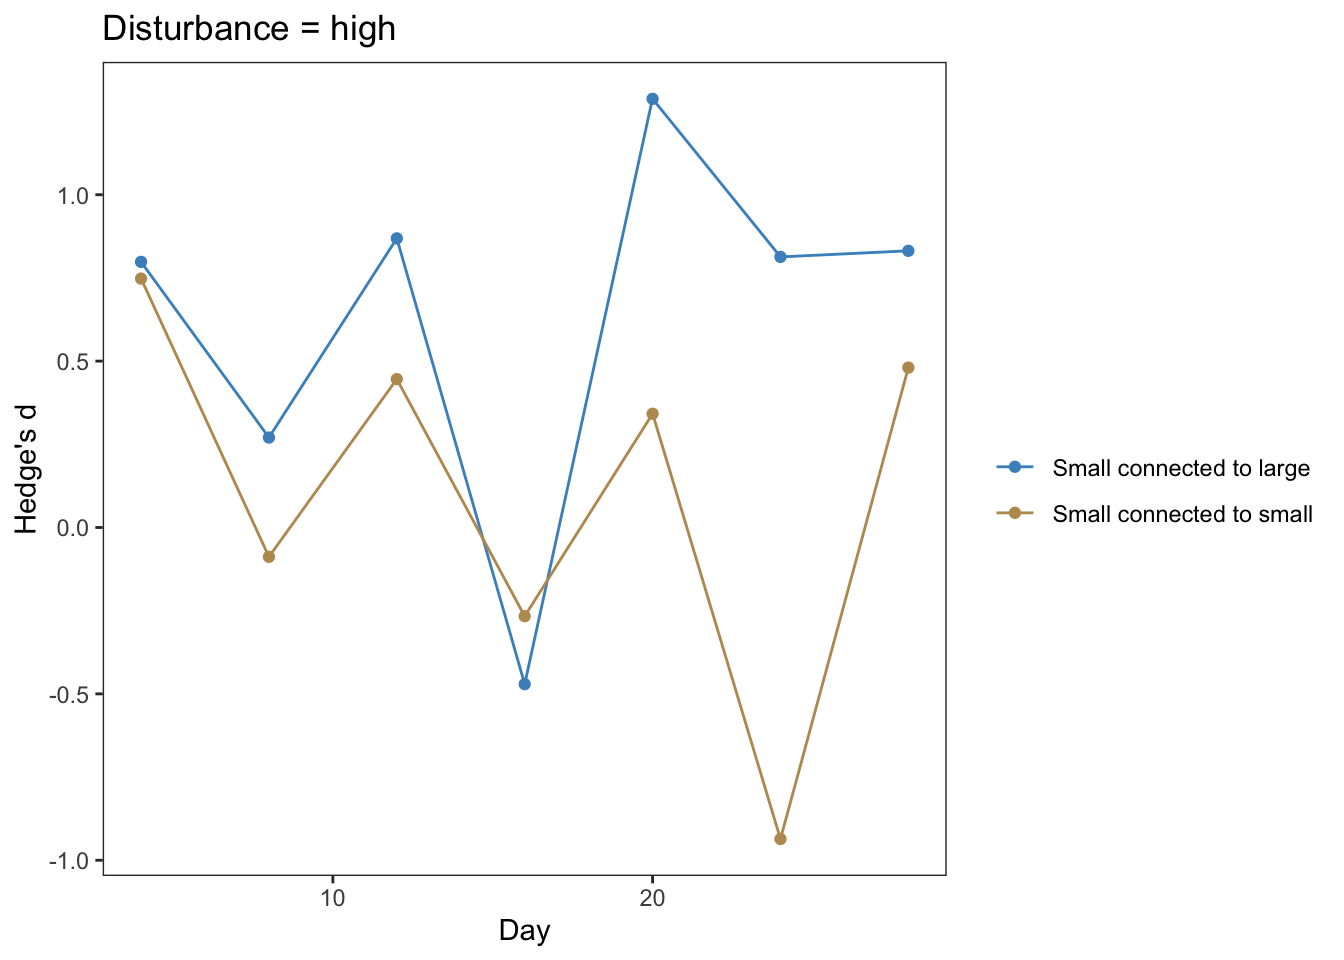
\includegraphics{index_files/figure-latex/unnamed-chunk-163-2.pdf}

\begin{Shaded}
\begin{Highlighting}[]
\NormalTok{model\_stats\_full }\OtherTok{=} \FunctionTok{compute.model.stats}\NormalTok{(full\_model,}
\NormalTok{                                       null\_model,}
                                       \StringTok{"mixed\_model"}\NormalTok{) }\SpecialCharTok{\%\textgreater{}\%}
  \FunctionTok{print}\NormalTok{()}
\end{Highlighting}
\end{Shaded}

\begin{verbatim}
##   deltaAIC   p_value R2
## 1 2.695563 0.5208889 NA
\end{verbatim}

\begin{itemize}
\tightlist
\item
  Interaction model (with \texttt{patch\_size\_symmetry:day})
\end{itemize}

\begin{Shaded}
\begin{Highlighting}[]
\NormalTok{interaction\_model }\OtherTok{=} \FunctionTok{lmer}\NormalTok{(}
  \FunctionTok{get}\NormalTok{(response\_variable) }\SpecialCharTok{\textasciitilde{}}
\NormalTok{    day }\SpecialCharTok{+} 
\NormalTok{    patch\_size\_symmetry }\SpecialCharTok{:}\NormalTok{ day }\SpecialCharTok{+} 
\NormalTok{    (day }\SpecialCharTok{|}\NormalTok{ system\_nr), }
  \AttributeTok{data =}\NormalTok{ filtered\_data,}
  \AttributeTok{REML =} \ConstantTok{FALSE}\NormalTok{,}
  \AttributeTok{control =} \FunctionTok{lmerControl}\NormalTok{(}\AttributeTok{optimizer =} \StringTok{"Nelder\_Mead"}\NormalTok{)}
\NormalTok{)}

\FunctionTok{summary}\NormalTok{(interaction\_model)}
\end{Highlighting}
\end{Shaded}

\begin{verbatim}
## Linear mixed model fit by maximum likelihood  ['lmerMod']
## Formula: get(response_variable) ~ day + patch_size_symmetry:day + (day |  
##     system_nr)
##    Data: filtered_data
## Control: lmerControl(optimizer = "Nelder_Mead")
## 
##      AIC      BIC   logLik deviance df.resid 
##    600.1    614.8   -293.1    586.1       53 
## 
## Scaled residuals: 
##      Min       1Q   Median       3Q      Max 
## -3.13504 -0.42711  0.03911  0.56709  2.24115 
## 
## Random effects:
##  Groups    Name        Variance Std.Dev. Corr 
##  system_nr (Intercept) 1269.765 35.634        
##            day            1.783  1.335   -0.96
##  Residual               831.373 28.834        
## Number of obs: 60, groups:  system_nr, 10
## 
## Fixed effects:
##                                  Estimate Std. Error t value
## (Intercept)                      256.7656    15.3959  16.678
## day                               -7.6089     0.7318 -10.397
## day:patch_size_symmetrysymmetric   0.3160     0.4914   0.643
## 
## Correlation of Fixed Effects:
##             (Intr) day   
## day         -0.880       
## dy:ptch_sz_  0.000 -0.336
\end{verbatim}

\begin{Shaded}
\begin{Highlighting}[]
\FunctionTok{plot}\NormalTok{(interaction\_model)}
\end{Highlighting}
\end{Shaded}

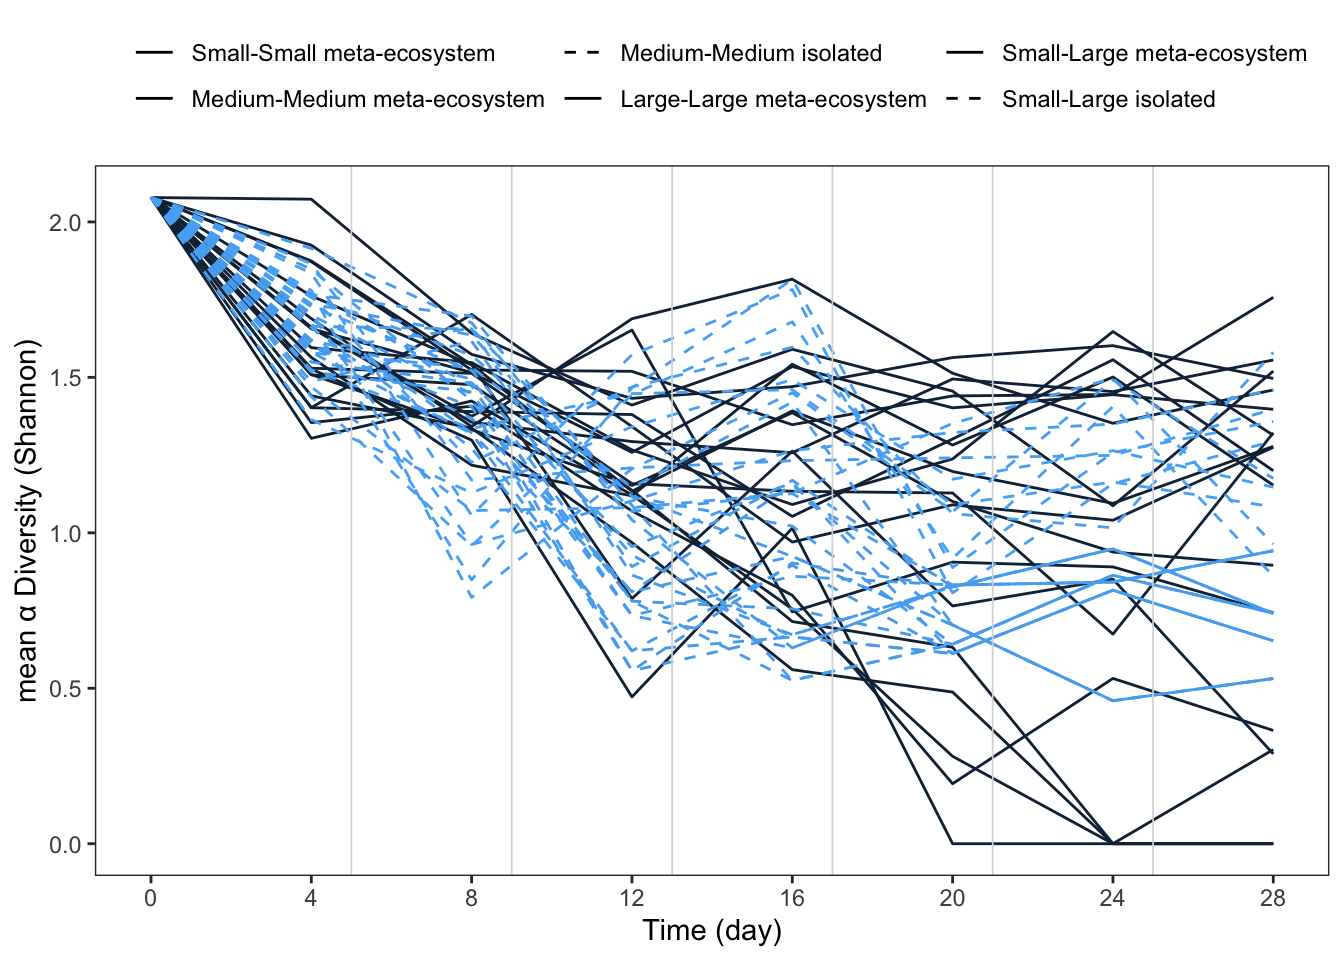
\includegraphics{index_files/figure-latex/unnamed-chunk-164-1.pdf}

\begin{Shaded}
\begin{Highlighting}[]
\FunctionTok{qqnorm}\NormalTok{(}\FunctionTok{resid}\NormalTok{(interaction\_model))}
\end{Highlighting}
\end{Shaded}

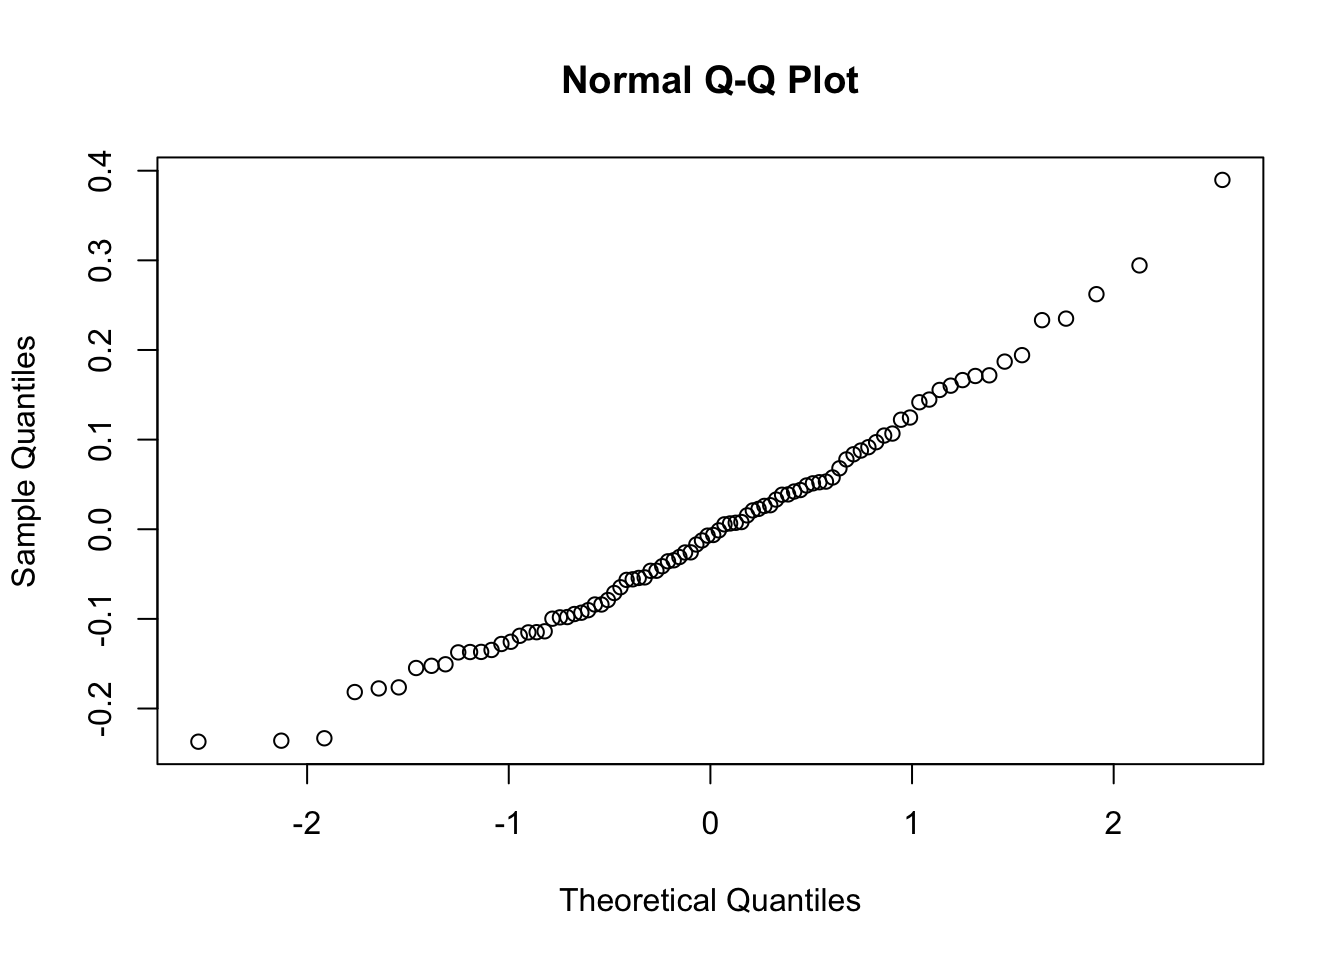
\includegraphics{index_files/figure-latex/unnamed-chunk-164-2.pdf}

\begin{Shaded}
\begin{Highlighting}[]
\NormalTok{model\_stats\_interaction }\OtherTok{=} \FunctionTok{compute.model.stats}\NormalTok{(interaction\_model,}
\NormalTok{                                              null\_model,}
                                              \StringTok{"mixed\_model"}\NormalTok{) }\SpecialCharTok{\%\textgreater{}\%}
  \FunctionTok{print}\NormalTok{()}
\end{Highlighting}
\end{Shaded}

\begin{verbatim}
##   deltaAIC   p_value R2
## 1 1.635225 0.5458665 NA
\end{verbatim}

\begin{itemize}
\tightlist
\item
  Fixed model (with \texttt{patch\_size\_symmetry})
\end{itemize}

\begin{Shaded}
\begin{Highlighting}[]
\NormalTok{fixed\_model }\OtherTok{=} \FunctionTok{lmer}\NormalTok{(}
  \FunctionTok{get}\NormalTok{(response\_variable) }\SpecialCharTok{\textasciitilde{}}
\NormalTok{    day }\SpecialCharTok{+} 
\NormalTok{    patch\_size\_symmetry }\SpecialCharTok{+} 
\NormalTok{    (day }\SpecialCharTok{|}\NormalTok{ system\_nr), }
  \AttributeTok{data =}\NormalTok{ filtered\_data,}
  \AttributeTok{REML =} \ConstantTok{FALSE}\NormalTok{,}
  \AttributeTok{control =} \FunctionTok{lmerControl}\NormalTok{(}\AttributeTok{optimizer =} \StringTok{"Nelder\_Mead"}\NormalTok{)}
\NormalTok{)}

\FunctionTok{summary}\NormalTok{(fixed\_model)}
\end{Highlighting}
\end{Shaded}

\begin{verbatim}
## Linear mixed model fit by maximum likelihood  ['lmerMod']
## Formula: get(response_variable) ~ day + patch_size_symmetry + (day | system_nr)
##    Data: filtered_data
## Control: lmerControl(optimizer = "Nelder_Mead")
## 
##      AIC      BIC   logLik deviance df.resid 
##    599.6    614.3   -292.8    585.6       53 
## 
## Scaled residuals: 
##     Min      1Q  Median      3Q     Max 
## -3.1638 -0.4251  0.0160  0.5549  2.2031 
## 
## Random effects:
##  Groups    Name        Variance Std.Dev. Corr 
##  system_nr (Intercept) 1130.828 33.628        
##            day            1.603  1.266   -0.95
##  Residual               831.372 28.834        
## Number of obs: 60, groups:  system_nr, 10
## 
## Fixed effects:
##                              Estimate Std. Error t value
## (Intercept)                  251.3493    15.9005  15.808
## day                           -7.4509     0.6762 -11.020
## patch_size_symmetrysymmetric  10.8327    10.8968   0.994
## 
## Correlation of Fixed Effects:
##             (Intr) day   
## day         -0.875       
## ptch_sz_sym -0.343  0.000
\end{verbatim}

\begin{Shaded}
\begin{Highlighting}[]
\FunctionTok{plot}\NormalTok{(fixed\_model)}
\end{Highlighting}
\end{Shaded}

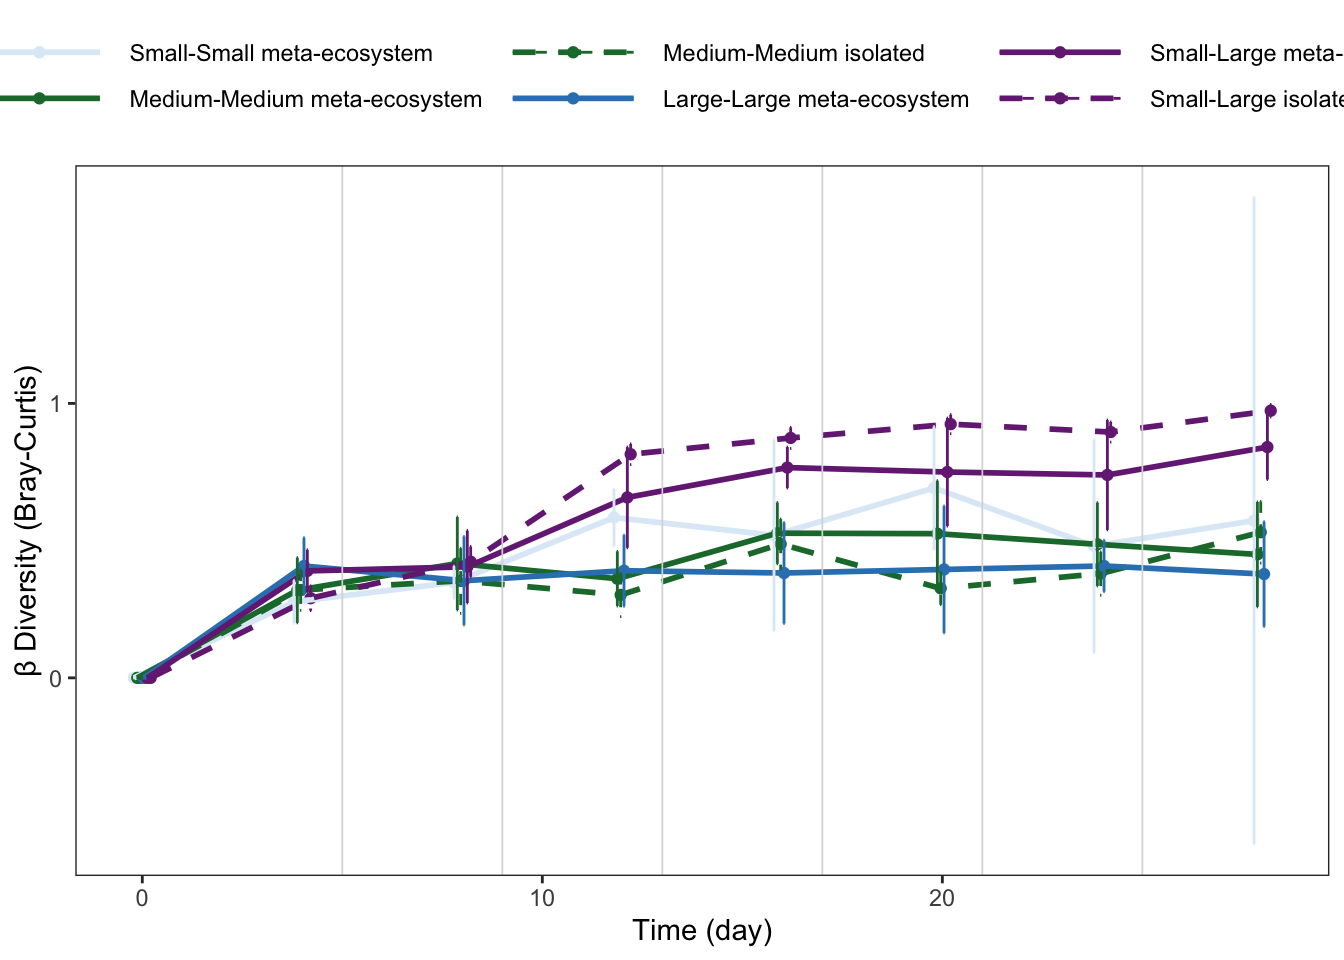
\includegraphics{index_files/figure-latex/unnamed-chunk-165-1.pdf}

\begin{Shaded}
\begin{Highlighting}[]
\FunctionTok{qqnorm}\NormalTok{(}\FunctionTok{resid}\NormalTok{(fixed\_model))}
\end{Highlighting}
\end{Shaded}

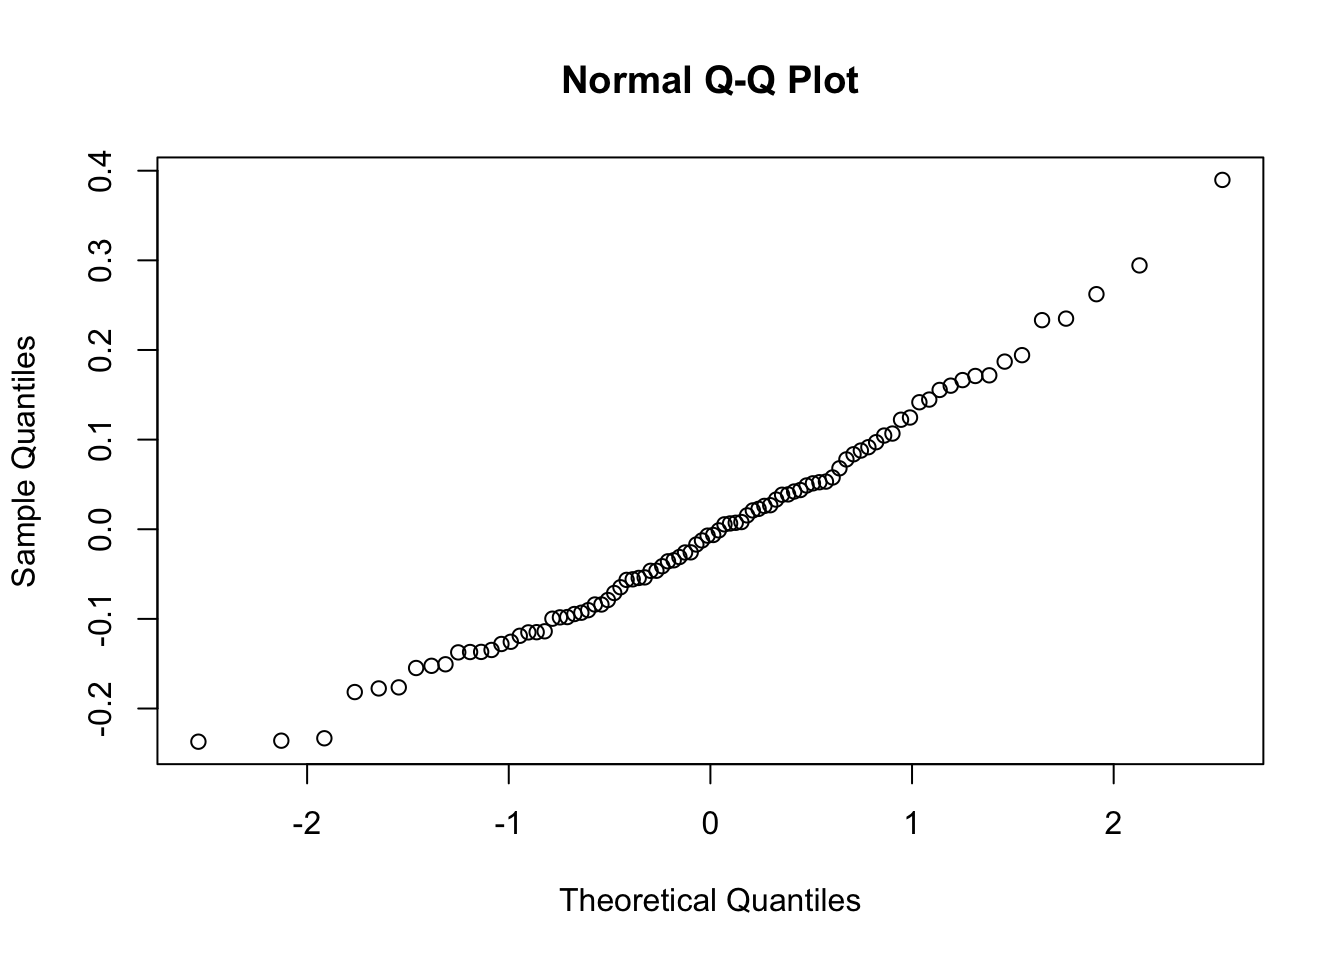
\includegraphics{index_files/figure-latex/unnamed-chunk-165-2.pdf}

\begin{Shaded}
\begin{Highlighting}[]
\NormalTok{model\_stats\_fixed }\OtherTok{=} \FunctionTok{compute.model.stats}\NormalTok{(fixed\_model,}
\NormalTok{                                              null\_model,}
                                              \StringTok{"mixed\_model"}\NormalTok{) }\SpecialCharTok{\%\textgreater{}\%}
  \FunctionTok{print}\NormalTok{()}
\end{Highlighting}
\end{Shaded}

\begin{verbatim}
##   deltaAIC   p_value R2
## 1 1.105268 0.3441981 NA
\end{verbatim}

\begin{Shaded}
\begin{Highlighting}[]
\NormalTok{results\_table }\OtherTok{=} \FunctionTok{fill.results.table}\NormalTok{(}
\NormalTok{  results\_table,}
\NormalTok{  response\_variable,}
\NormalTok{  metaecosystem\_type\_input\_model,}
\NormalTok{  model\_stats\_full,}
\NormalTok{  model\_stats\_interaction,}
\NormalTok{  model\_stats\_fixed}
\NormalTok{)}
\end{Highlighting}
\end{Shaded}

Small-Large connected vs isolated

\begin{Shaded}
\begin{Highlighting}[]
\NormalTok{metaecosystem\_type\_input\_model }\OtherTok{=} \FunctionTok{c}\NormalTok{(}\StringTok{"Small{-}Large meta{-}ecosystem"}\NormalTok{,}
                                   \StringTok{"Small{-}Large isolated"}\NormalTok{)}
\end{Highlighting}
\end{Shaded}

\begin{Shaded}
\begin{Highlighting}[]
\CommentTok{\#Compute stats for all patch combinations }
\NormalTok{isolated\_combinations\_sets\_filtered }\OtherTok{=}\NormalTok{  isolated\_combinations\_sets }\SpecialCharTok{\%\textgreater{}\%}
  \FunctionTok{filter}\NormalTok{(disturbance }\SpecialCharTok{==}\NormalTok{ disturbance\_global\_input,}
\NormalTok{         metaecosystem\_type }\SpecialCharTok{\%in\%}\NormalTok{ metaecosystem\_type\_input\_model)}

\NormalTok{n\_sets }\OtherTok{=}\NormalTok{ isolated\_combinations\_sets\_filtered }\SpecialCharTok{\%\textgreater{}\%}
  \FunctionTok{pull}\NormalTok{(set) }\SpecialCharTok{\%\textgreater{}\%}
  \FunctionTok{max}\NormalTok{()}

\ControlFlowTok{for}\NormalTok{ (set\_input }\ControlFlowTok{in} \DecValTok{1}\SpecialCharTok{:}\NormalTok{n\_sets) \{}
  
\NormalTok{  system\_nr\_isolated\_systems }\OtherTok{=}\NormalTok{ isolated\_combinations\_sets\_filtered }\SpecialCharTok{\%\textgreater{}\%}
    \FunctionTok{filter}\NormalTok{(}
\NormalTok{      metaecosystem\_type }\SpecialCharTok{\%in\%}\NormalTok{ metaecosystem\_type\_input\_model,}
\NormalTok{      connection }\SpecialCharTok{==} \StringTok{"isolated"}\NormalTok{,}
\NormalTok{      set }\SpecialCharTok{==}\NormalTok{ set\_input}
\NormalTok{    ) }\SpecialCharTok{\%\textgreater{}\%}
    \FunctionTok{pull}\NormalTok{(system\_nr)}
  
\NormalTok{  filtered\_data }\OtherTok{=}\NormalTok{ ds\_metaecosystems }\SpecialCharTok{\%\textgreater{}\%}
    \FunctionTok{filter}\NormalTok{(}
\NormalTok{      time\_point }\SpecialCharTok{\textgreater{}=}\NormalTok{ first\_time\_point\_model,}
\NormalTok{      time\_point }\SpecialCharTok{\textless{}=}\NormalTok{ last\_time\_point\_model,}
\NormalTok{      metaecosystem\_type }\SpecialCharTok{\%in\%}\NormalTok{ metaecosystem\_type\_input\_model,}
\NormalTok{      connection }\SpecialCharTok{==} \StringTok{"connected"} \SpecialCharTok{|}
\NormalTok{        (connection }\SpecialCharTok{==} \StringTok{"isolated"} \SpecialCharTok{\&}
\NormalTok{           system\_nr }\SpecialCharTok{\%in\%}\NormalTok{ system\_nr\_isolated\_systems)}
\NormalTok{    )}
  
\NormalTok{  null\_model }\OtherTok{=} \FunctionTok{lmer}\NormalTok{(}
    \FunctionTok{get}\NormalTok{(response\_variable) }\SpecialCharTok{\textasciitilde{}}
\NormalTok{      day }\SpecialCharTok{+}
\NormalTok{      (day }\SpecialCharTok{|}\NormalTok{ system\_nr),}
    \AttributeTok{data =}\NormalTok{ filtered\_data,}
    \AttributeTok{REML =} \ConstantTok{FALSE}\NormalTok{,}
    \AttributeTok{control =} \FunctionTok{lmerControl}\NormalTok{(}\AttributeTok{optimizer =} \StringTok{"Nelder\_Mead"}\NormalTok{)}
\NormalTok{  )}
  
\NormalTok{  full\_model }\OtherTok{=} \FunctionTok{lmer}\NormalTok{(}
    \FunctionTok{get}\NormalTok{(response\_variable) }\SpecialCharTok{\textasciitilde{}}
\NormalTok{      day }\SpecialCharTok{+}
\NormalTok{      connection }\SpecialCharTok{+}
\NormalTok{      connection}\SpecialCharTok{:}\NormalTok{day }\SpecialCharTok{+}
\NormalTok{      (day }\SpecialCharTok{|}\NormalTok{ system\_nr),}
    \AttributeTok{data =}\NormalTok{ filtered\_data,}
    \AttributeTok{REML =} \ConstantTok{FALSE}\NormalTok{,}
    \AttributeTok{control =} \FunctionTok{lmerControl}\NormalTok{(}\AttributeTok{optimizer =} \StringTok{"Nelder\_Mead"}\NormalTok{)}
\NormalTok{  )}
  
\NormalTok{  model\_stats\_full }\OtherTok{=} \FunctionTok{compute.model.stats}\NormalTok{(full\_model,}
\NormalTok{                                         null\_model,}
                                         \StringTok{"mixed\_model"}\NormalTok{)}
  
\NormalTok{  interaction\_model }\OtherTok{=} \FunctionTok{lmer}\NormalTok{(}
    \FunctionTok{get}\NormalTok{(response\_variable) }\SpecialCharTok{\textasciitilde{}}
\NormalTok{      day }\SpecialCharTok{+}
\NormalTok{      connection}\SpecialCharTok{:}\NormalTok{day }\SpecialCharTok{+}
\NormalTok{      (day }\SpecialCharTok{|}\NormalTok{ system\_nr),}
    \AttributeTok{data =}\NormalTok{ filtered\_data,}
    \AttributeTok{REML =} \ConstantTok{FALSE}\NormalTok{,}
    \AttributeTok{control =} \FunctionTok{lmerControl}\NormalTok{(}\AttributeTok{optimizer =} \StringTok{"Nelder\_Mead"}\NormalTok{)}
\NormalTok{  )}
  
\NormalTok{  model\_stats\_interaction }\OtherTok{=} \FunctionTok{compute.model.stats}\NormalTok{(interaction\_model,}
\NormalTok{                                                null\_model,}
                                                \StringTok{"mixed\_model"}\NormalTok{)}
  
\NormalTok{  fixed\_model }\OtherTok{=} \FunctionTok{lmer}\NormalTok{(}
    \FunctionTok{get}\NormalTok{(response\_variable) }\SpecialCharTok{\textasciitilde{}}
\NormalTok{      day }\SpecialCharTok{+}
\NormalTok{      connection }\SpecialCharTok{+}
\NormalTok{      (day }\SpecialCharTok{|}\NormalTok{ system\_nr),}
    \AttributeTok{data =}\NormalTok{ filtered\_data,}
    \AttributeTok{REML =} \ConstantTok{FALSE}\NormalTok{,}
    \AttributeTok{control =} \FunctionTok{lmerControl}\NormalTok{(}\AttributeTok{optimizer =} \StringTok{"Nelder\_Mead"}\NormalTok{)}
\NormalTok{  )}
  
\NormalTok{  model\_stats\_fixed }\OtherTok{=} \FunctionTok{compute.model.stats}\NormalTok{(fixed\_model,}
\NormalTok{                                          null\_model,}
                                          \StringTok{"mixed\_model"}\NormalTok{)}
  
\NormalTok{  iterated\_results\_table }\OtherTok{=} \FunctionTok{fill.results.table}\NormalTok{(}
\NormalTok{    iterated\_results\_table,}
\NormalTok{    response\_variable,}
\NormalTok{    metaecosystem\_type\_input\_model,}
\NormalTok{    model\_stats\_full,}
\NormalTok{    model\_stats\_interaction,}
\NormalTok{    model\_stats\_fixed}
\NormalTok{  )}
  
\NormalTok{  iterated\_results\_table}\SpecialCharTok{$}\NormalTok{set }\OtherTok{=}\NormalTok{ set\_input}
\NormalTok{\}}
\end{Highlighting}
\end{Shaded}

\begin{verbatim}
## Warning in checkConv(attr(opt, "derivs"), opt$par, ctrl = control$checkConv, :
## Model failed to converge with max|grad| = 3.51228 (tol = 0.002, component 1)
\end{verbatim}

\begin{Shaded}
\begin{Highlighting}[]
\CommentTok{\#Check that there\textquotesingle{}s nothing wired with the AIC and p{-}value distributions }
\FunctionTok{hist}\NormalTok{(iterated\_results\_table}\SpecialCharTok{$}\NormalTok{ΔAIC\_full, }\AttributeTok{main =} \StringTok{"Distribution of ΔAIC of the full model."}\NormalTok{) }
\end{Highlighting}
\end{Shaded}

\begin{verbatim}
## Warning in title(main = main, sub = sub, xlab = xlab, ylab = ylab, ...):
## conversion failure on 'Distribution of ΔAIC of the full model.' in 'mbcsToSbcs':
## dot substituted for <ce>
\end{verbatim}

\begin{verbatim}
## Warning in title(main = main, sub = sub, xlab = xlab, ylab = ylab, ...):
## conversion failure on 'Distribution of ΔAIC of the full model.' in 'mbcsToSbcs':
## dot substituted for <94>
\end{verbatim}

\begin{verbatim}
## Warning in title(main = main, sub = sub, xlab = xlab, ylab = ylab, ...):
## conversion failure on 'iterated_results_table$ΔAIC_full' in 'mbcsToSbcs': dot
## substituted for <ce>
\end{verbatim}

\begin{verbatim}
## Warning in title(main = main, sub = sub, xlab = xlab, ylab = ylab, ...):
## conversion failure on 'iterated_results_table$ΔAIC_full' in 'mbcsToSbcs': dot
## substituted for <94>
\end{verbatim}

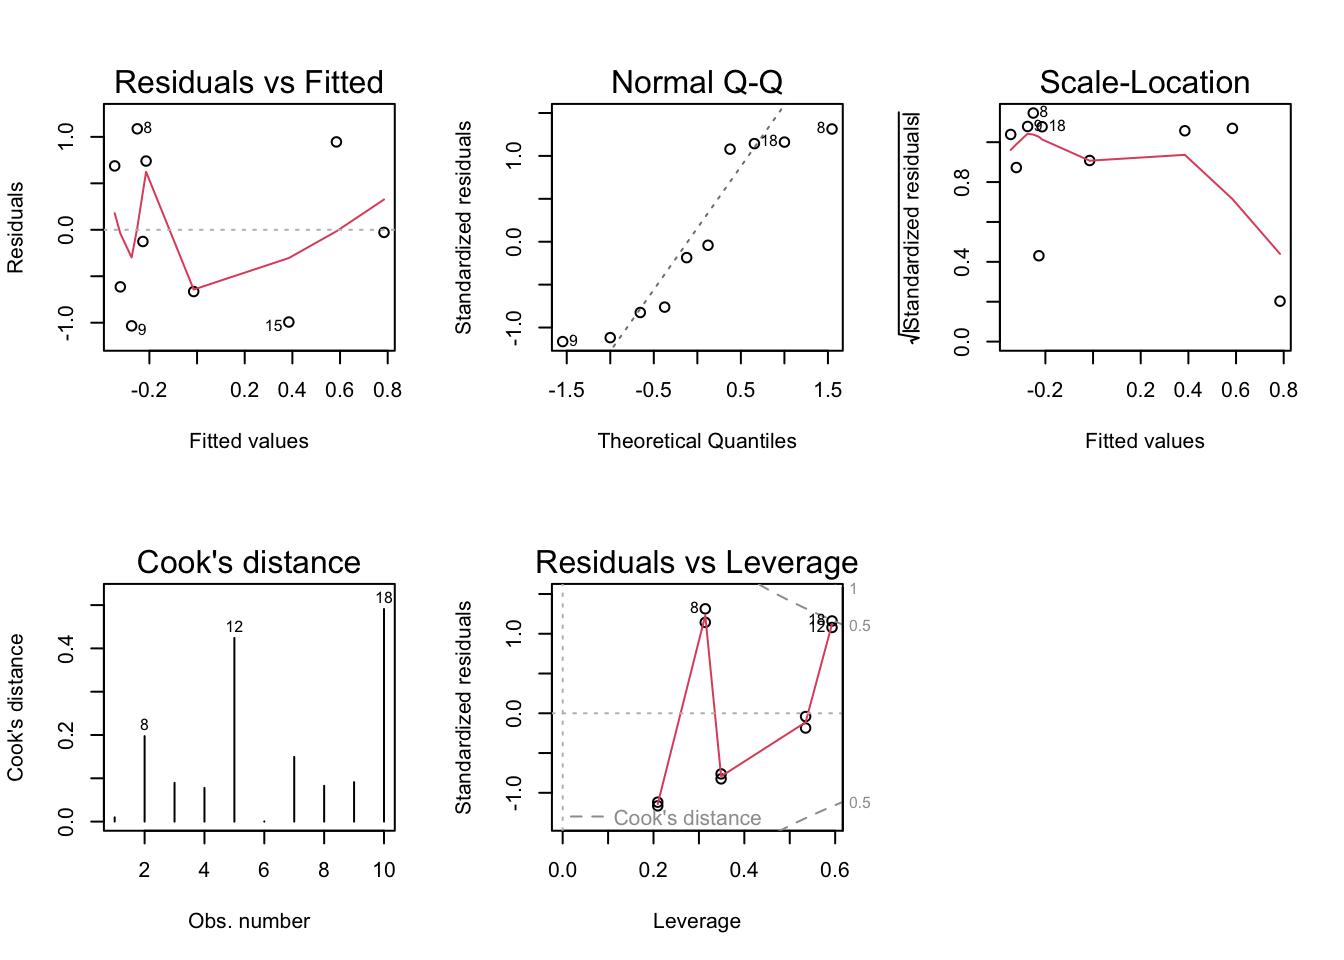
\includegraphics{index_files/figure-latex/unnamed-chunk-168-1.pdf}

\begin{Shaded}
\begin{Highlighting}[]
\FunctionTok{hist}\NormalTok{(iterated\_results\_table}\SpecialCharTok{$}\NormalTok{p\_full, }\AttributeTok{main =} \StringTok{"Distribution of p{-}values of the full model."}\NormalTok{) }
\end{Highlighting}
\end{Shaded}

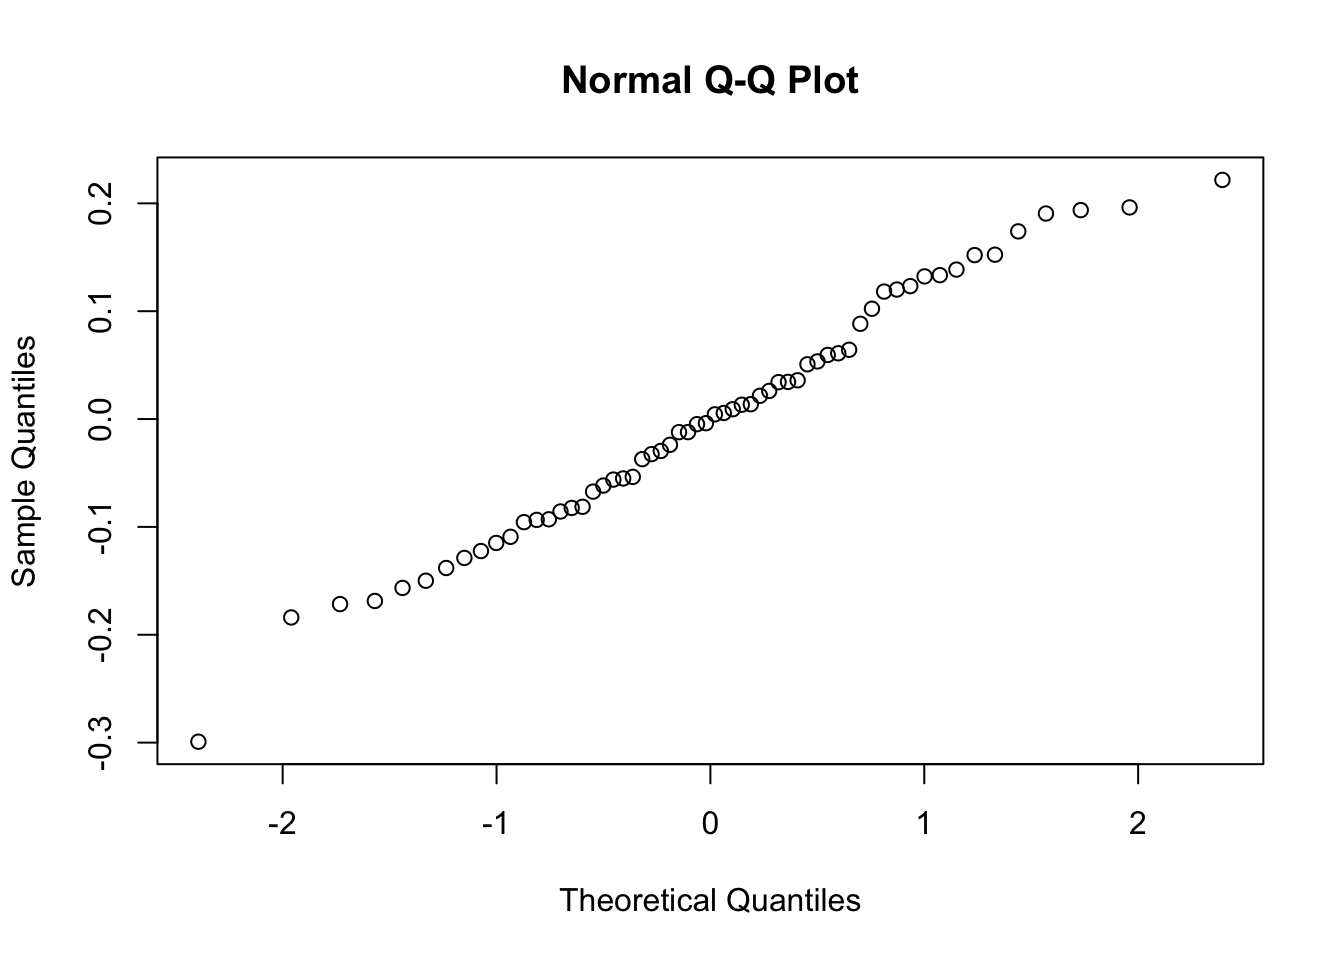
\includegraphics{index_files/figure-latex/unnamed-chunk-168-2.pdf}

\begin{Shaded}
\begin{Highlighting}[]
\FunctionTok{hist}\NormalTok{(iterated\_results\_table}\SpecialCharTok{$}\NormalTok{ΔAIC\_fix, }\AttributeTok{main =} \StringTok{"Distribution of ΔAIC of the fixed model."}\NormalTok{) }
\end{Highlighting}
\end{Shaded}

\begin{verbatim}
## Warning in title(main = main, sub = sub, xlab = xlab, ylab = ylab, ...):
## conversion failure on 'Distribution of ΔAIC of the fixed model.' in
## 'mbcsToSbcs': dot substituted for <ce>
\end{verbatim}

\begin{verbatim}
## Warning in title(main = main, sub = sub, xlab = xlab, ylab = ylab, ...):
## conversion failure on 'Distribution of ΔAIC of the fixed model.' in
## 'mbcsToSbcs': dot substituted for <94>
\end{verbatim}

\begin{verbatim}
## Warning in title(main = main, sub = sub, xlab = xlab, ylab = ylab, ...):
## conversion failure on 'iterated_results_table$ΔAIC_fix' in 'mbcsToSbcs': dot
## substituted for <ce>
\end{verbatim}

\begin{verbatim}
## Warning in title(main = main, sub = sub, xlab = xlab, ylab = ylab, ...):
## conversion failure on 'iterated_results_table$ΔAIC_fix' in 'mbcsToSbcs': dot
## substituted for <94>
\end{verbatim}

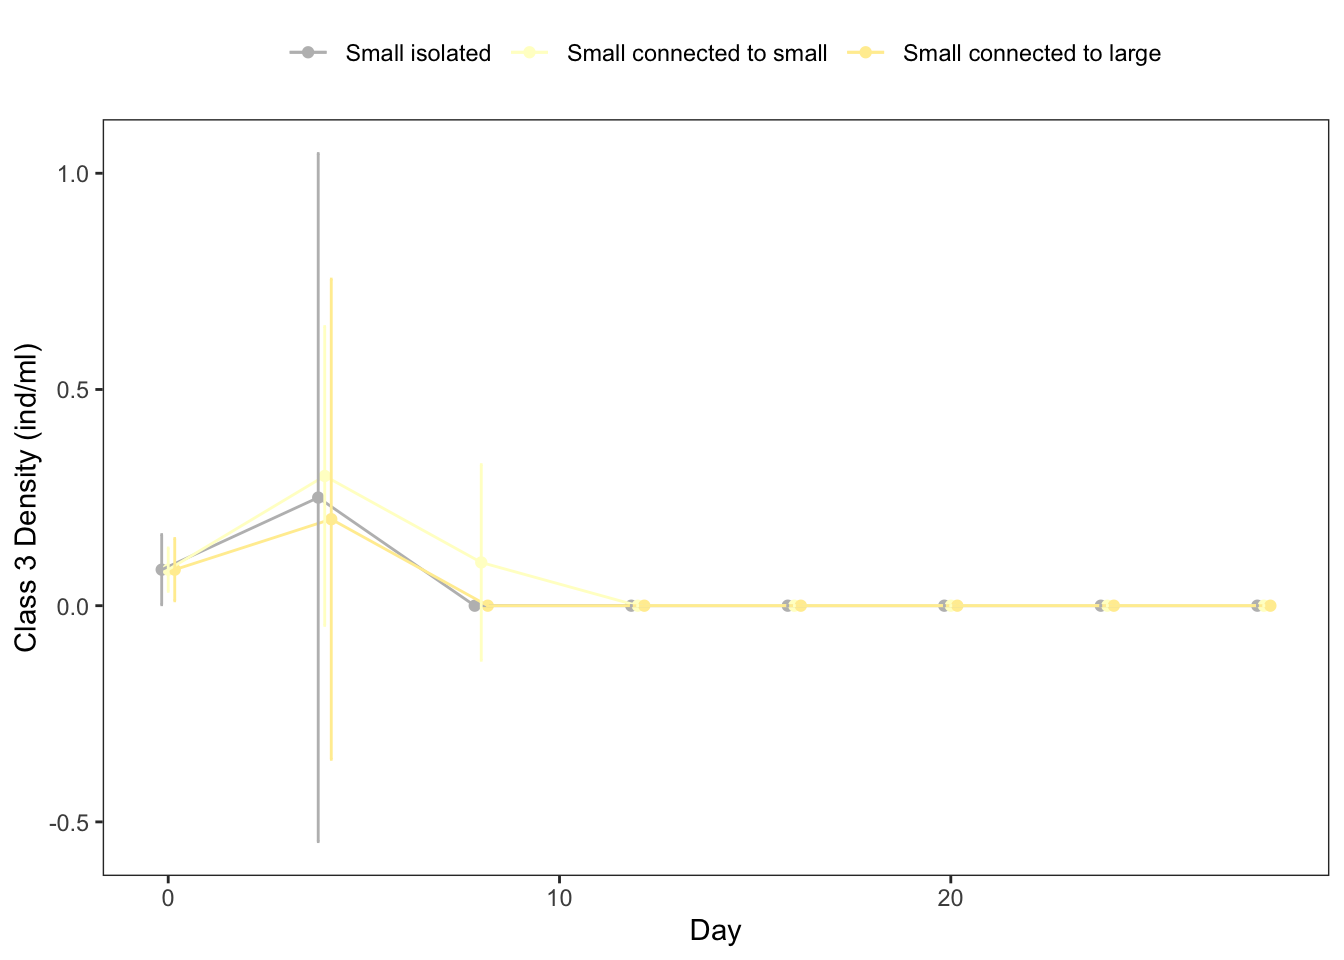
\includegraphics{index_files/figure-latex/unnamed-chunk-168-3.pdf}

\begin{Shaded}
\begin{Highlighting}[]
\FunctionTok{hist}\NormalTok{(iterated\_results\_table}\SpecialCharTok{$}\NormalTok{p\_fix, }\AttributeTok{main =} \StringTok{"Distribution of p{-}values of the fixed model."}\NormalTok{) }
\end{Highlighting}
\end{Shaded}

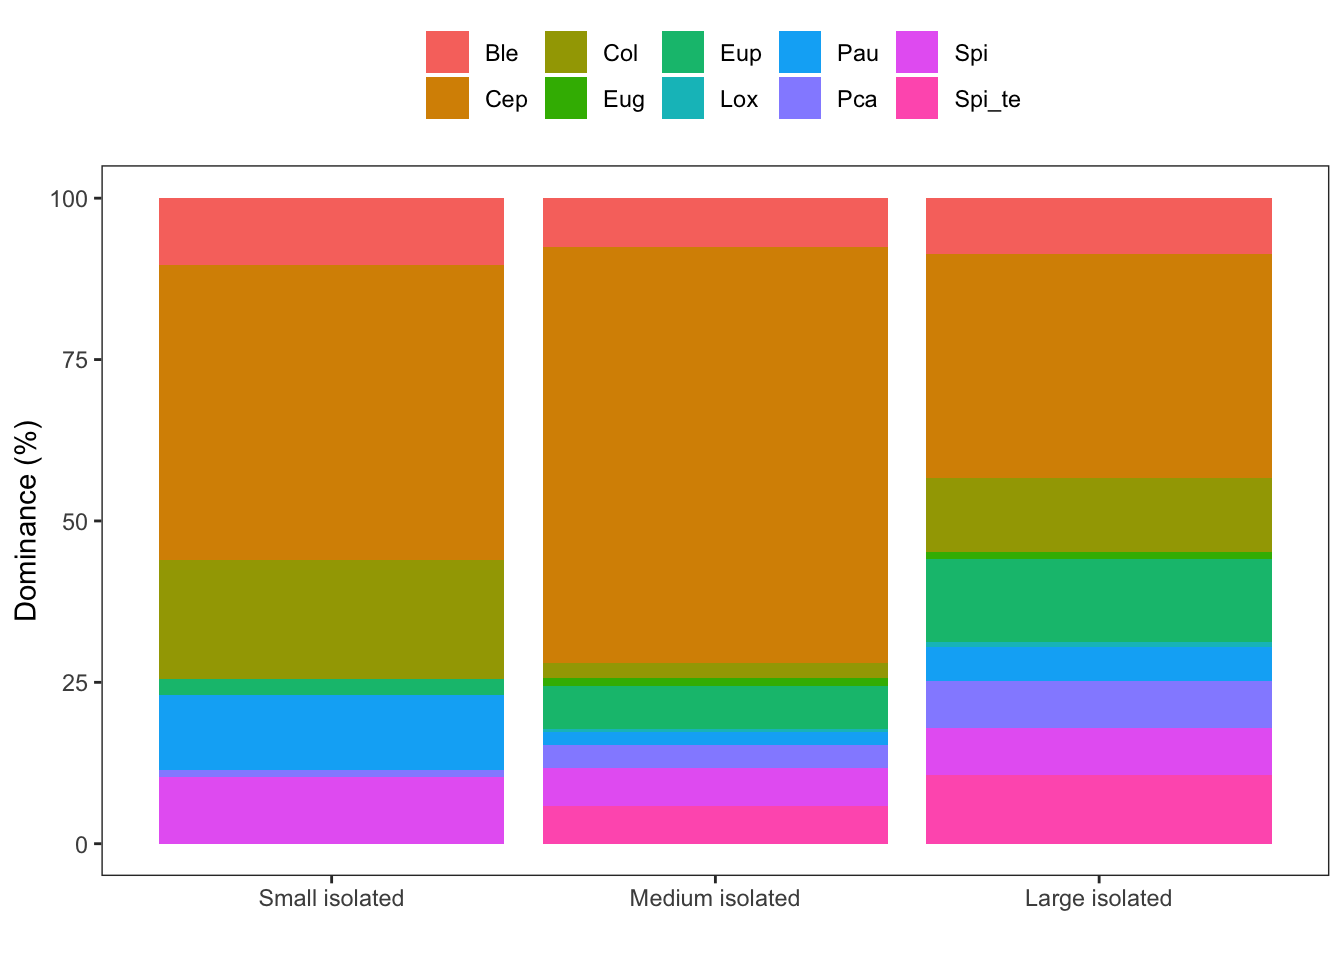
\includegraphics{index_files/figure-latex/unnamed-chunk-168-4.pdf}

\begin{Shaded}
\begin{Highlighting}[]
\FunctionTok{hist}\NormalTok{(iterated\_results\_table}\SpecialCharTok{$}\NormalTok{ΔAIC\_int, }\AttributeTok{main =} \StringTok{"Distribution of ΔAIC of the interation model."}\NormalTok{) }
\end{Highlighting}
\end{Shaded}

\begin{verbatim}
## Warning in title(main = main, sub = sub, xlab = xlab, ylab = ylab, ...):
## conversion failure on 'Distribution of ΔAIC of the interation model.' in
## 'mbcsToSbcs': dot substituted for <ce>
\end{verbatim}

\begin{verbatim}
## Warning in title(main = main, sub = sub, xlab = xlab, ylab = ylab, ...):
## conversion failure on 'Distribution of ΔAIC of the interation model.' in
## 'mbcsToSbcs': dot substituted for <94>
\end{verbatim}

\begin{verbatim}
## Warning in title(main = main, sub = sub, xlab = xlab, ylab = ylab, ...):
## conversion failure on 'iterated_results_table$ΔAIC_int' in 'mbcsToSbcs': dot
## substituted for <ce>
\end{verbatim}

\begin{verbatim}
## Warning in title(main = main, sub = sub, xlab = xlab, ylab = ylab, ...):
## conversion failure on 'iterated_results_table$ΔAIC_int' in 'mbcsToSbcs': dot
## substituted for <94>
\end{verbatim}

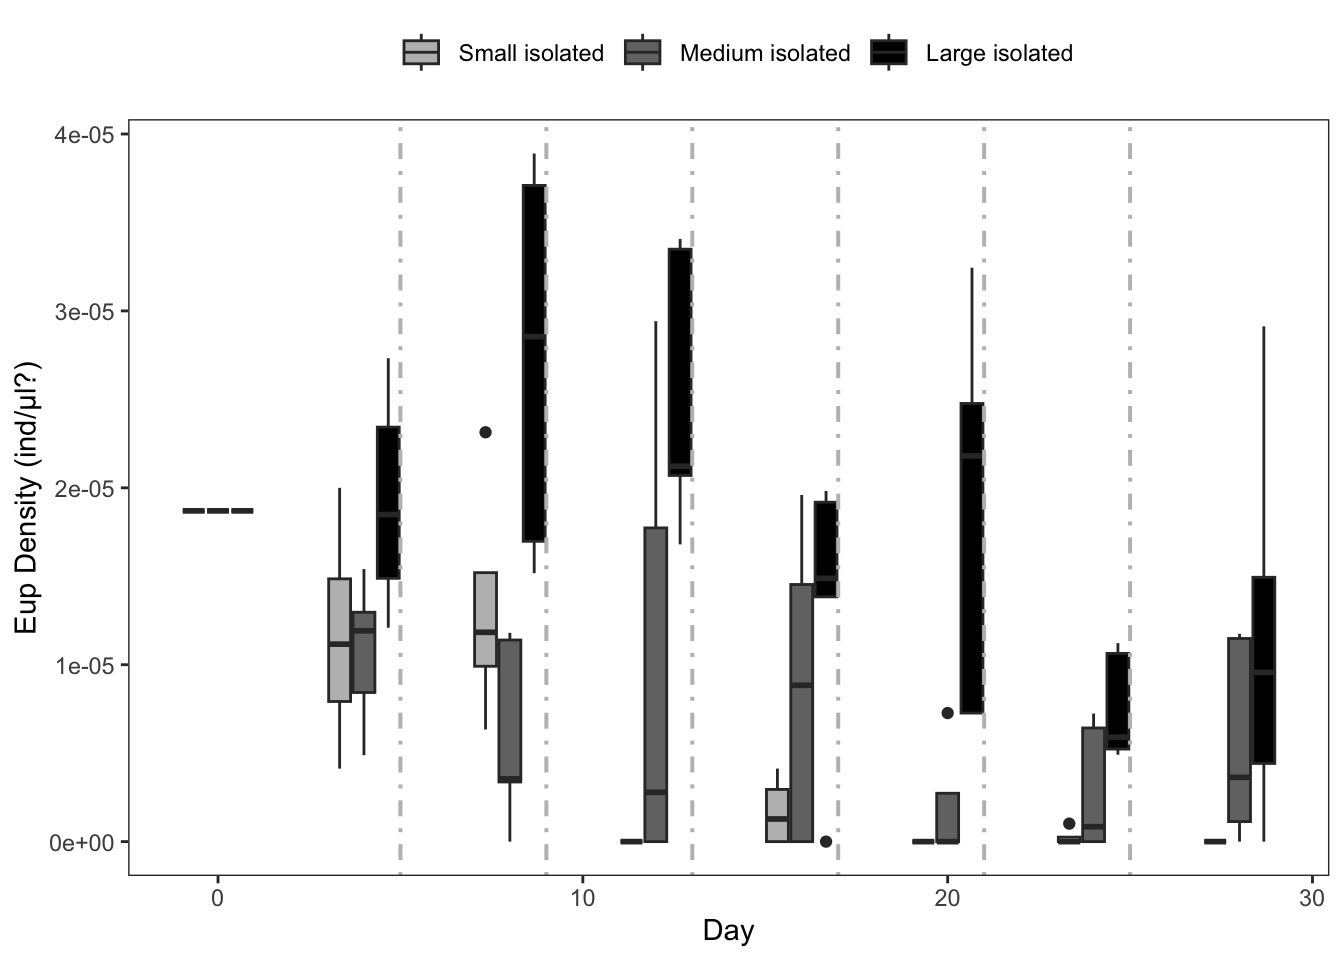
\includegraphics{index_files/figure-latex/unnamed-chunk-168-5.pdf}

\begin{Shaded}
\begin{Highlighting}[]
\FunctionTok{hist}\NormalTok{(iterated\_results\_table}\SpecialCharTok{$}\NormalTok{p\_int, }\AttributeTok{main =} \StringTok{"Distribution of p{-}values of the interation model."}\NormalTok{) }
\end{Highlighting}
\end{Shaded}

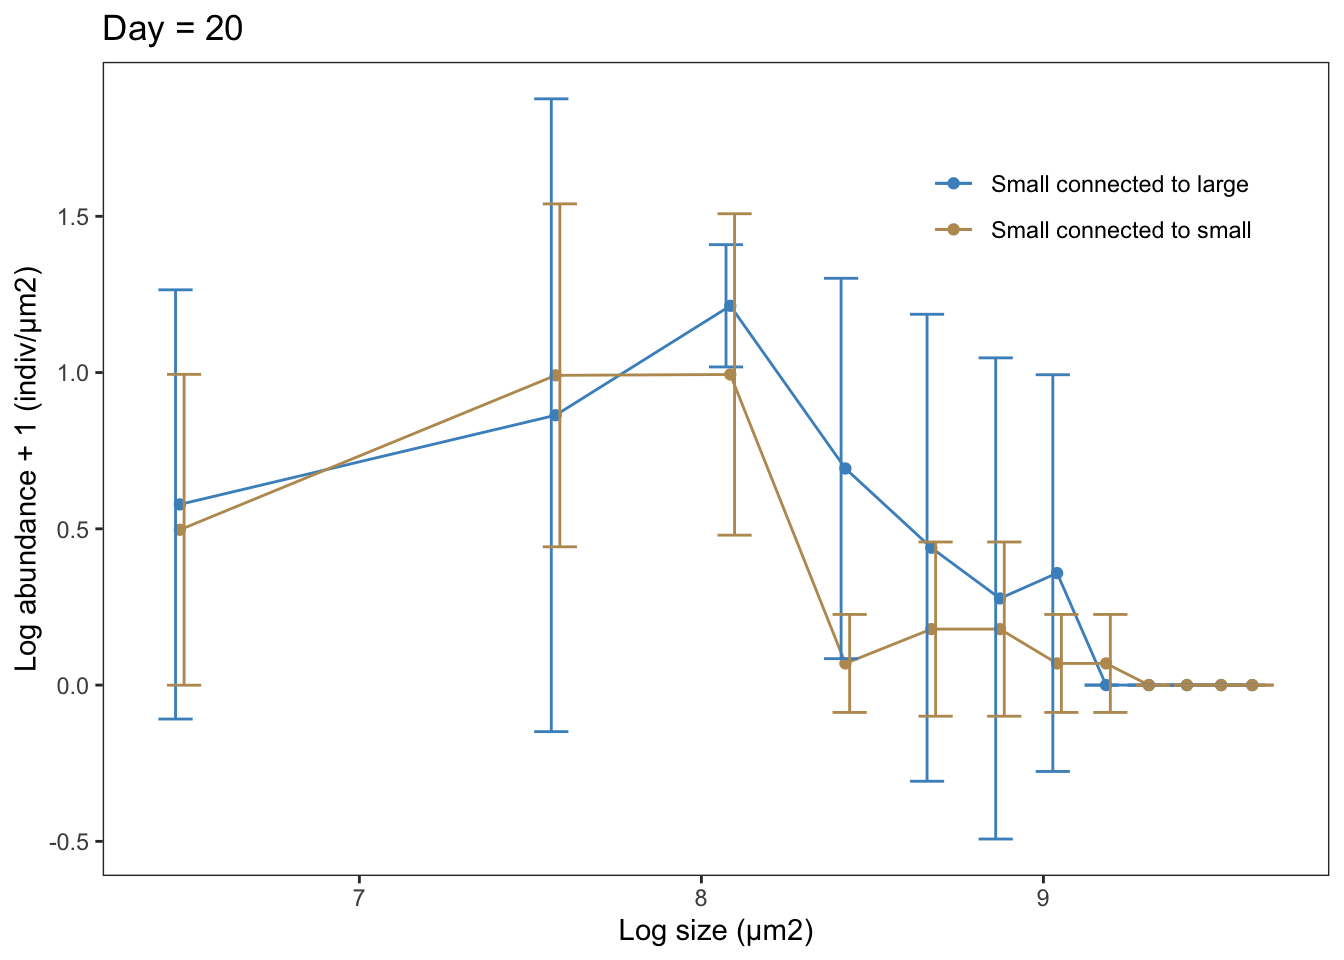
\includegraphics{index_files/figure-latex/unnamed-chunk-168-6.pdf}

\begin{Shaded}
\begin{Highlighting}[]
\CommentTok{\#Use the mean p{-}values and ΔAIC }
\NormalTok{model\_stats\_full }\OtherTok{=} \FunctionTok{data.frame}\NormalTok{(}
  \AttributeTok{deltaAIC =} \FunctionTok{mean}\NormalTok{(iterated\_results\_table}\SpecialCharTok{$}\NormalTok{ΔAIC\_full),}
  \AttributeTok{p\_value =} \FunctionTok{mean}\NormalTok{(iterated\_results\_table}\SpecialCharTok{$}\NormalTok{p\_full),}
  \AttributeTok{R2 =} \ConstantTok{NA}
\NormalTok{) }

\NormalTok{model\_stats\_interaction }\OtherTok{=} \FunctionTok{data.frame}\NormalTok{(}
  \AttributeTok{deltaAIC =} \FunctionTok{mean}\NormalTok{(iterated\_results\_table}\SpecialCharTok{$}\NormalTok{ΔAIC\_int),}
  \AttributeTok{p\_value =} \FunctionTok{mean}\NormalTok{(iterated\_results\_table}\SpecialCharTok{$}\NormalTok{p\_int),}
  \AttributeTok{R2 =} \ConstantTok{NA}
\NormalTok{)}

\NormalTok{model\_stats\_fixed }\OtherTok{=} \FunctionTok{data.frame}\NormalTok{(}
  \AttributeTok{deltaAIC =} \FunctionTok{mean}\NormalTok{(iterated\_results\_table}\SpecialCharTok{$}\NormalTok{ΔAIC\_fix),}
  \AttributeTok{p\_value =} \FunctionTok{mean}\NormalTok{(iterated\_results\_table}\SpecialCharTok{$}\NormalTok{p\_fix),}
  \AttributeTok{R2 =} \ConstantTok{NA}
\NormalTok{)}

\NormalTok{results\_table }\OtherTok{=} \FunctionTok{fill.results.table}\NormalTok{(}
\NormalTok{    results\_table,}
\NormalTok{    response\_variable,}
\NormalTok{    metaecosystem\_type\_input\_model,}
\NormalTok{    model\_stats\_full,}
\NormalTok{    model\_stats\_interaction,}
\NormalTok{    model\_stats\_fixed}
\NormalTok{  )}
\end{Highlighting}
\end{Shaded}

Medium-Medium connected vs isolated

\begin{Shaded}
\begin{Highlighting}[]
\NormalTok{metaecosystem\_type\_input\_model }\OtherTok{=} \FunctionTok{c}\NormalTok{(}\StringTok{"Medium{-}Medium meta{-}ecosystem"}\NormalTok{,}
                                   \StringTok{"Medium{-}Medium isolated"}\NormalTok{)}
\end{Highlighting}
\end{Shaded}

\begin{Shaded}
\begin{Highlighting}[]
\CommentTok{\#Compute stats for all patch combinations }
\NormalTok{isolated\_combinations\_sets\_filtered }\OtherTok{=}\NormalTok{  isolated\_combinations\_sets }\SpecialCharTok{\%\textgreater{}\%}
  \FunctionTok{filter}\NormalTok{(disturbance }\SpecialCharTok{==}\NormalTok{ disturbance\_global\_input,}
\NormalTok{         metaecosystem\_type }\SpecialCharTok{\%in\%}\NormalTok{ metaecosystem\_type\_input\_model)}

\NormalTok{n\_sets }\OtherTok{=}\NormalTok{ isolated\_combinations\_sets\_filtered }\SpecialCharTok{\%\textgreater{}\%}
  \FunctionTok{pull}\NormalTok{(set) }\SpecialCharTok{\%\textgreater{}\%}
  \FunctionTok{max}\NormalTok{()}

\ControlFlowTok{for}\NormalTok{ (set\_input }\ControlFlowTok{in} \DecValTok{1}\SpecialCharTok{:}\NormalTok{n\_sets) \{}
  
\NormalTok{  system\_nr\_isolated\_systems }\OtherTok{=}\NormalTok{ isolated\_combinations\_sets\_filtered }\SpecialCharTok{\%\textgreater{}\%}
    \FunctionTok{filter}\NormalTok{(}
\NormalTok{      metaecosystem\_type }\SpecialCharTok{\%in\%}\NormalTok{ metaecosystem\_type\_input\_model,}
\NormalTok{      connection }\SpecialCharTok{==} \StringTok{"isolated"}\NormalTok{,}
\NormalTok{      set }\SpecialCharTok{==}\NormalTok{ set\_input}
\NormalTok{    ) }\SpecialCharTok{\%\textgreater{}\%}
    \FunctionTok{pull}\NormalTok{(system\_nr)}
  
\NormalTok{  filtered\_data }\OtherTok{=}\NormalTok{ ds\_metaecosystems }\SpecialCharTok{\%\textgreater{}\%}
    \FunctionTok{filter}\NormalTok{(}
\NormalTok{      time\_point }\SpecialCharTok{\textgreater{}=}\NormalTok{ first\_time\_point\_model,}
\NormalTok{      time\_point }\SpecialCharTok{\textless{}=}\NormalTok{ last\_time\_point\_model,}
\NormalTok{      metaecosystem\_type }\SpecialCharTok{\%in\%}\NormalTok{ metaecosystem\_type\_input\_model,}
\NormalTok{      connection }\SpecialCharTok{==} \StringTok{"connected"} \SpecialCharTok{|}
\NormalTok{        (connection }\SpecialCharTok{==} \StringTok{"isolated"} \SpecialCharTok{\&}
\NormalTok{           system\_nr }\SpecialCharTok{\%in\%}\NormalTok{ system\_nr\_isolated\_systems)}
\NormalTok{    )}
  
\NormalTok{  null\_model }\OtherTok{=} \FunctionTok{lmer}\NormalTok{(}
    \FunctionTok{get}\NormalTok{(response\_variable) }\SpecialCharTok{\textasciitilde{}}
\NormalTok{      day }\SpecialCharTok{+}
\NormalTok{      (day }\SpecialCharTok{|}\NormalTok{ system\_nr),}
    \AttributeTok{data =}\NormalTok{ filtered\_data,}
    \AttributeTok{REML =} \ConstantTok{FALSE}\NormalTok{,}
    \AttributeTok{control =} \FunctionTok{lmerControl}\NormalTok{(}\AttributeTok{optimizer =} \StringTok{"Nelder\_Mead"}\NormalTok{)}
\NormalTok{  )}
  
\NormalTok{  full\_model }\OtherTok{=} \FunctionTok{lmer}\NormalTok{(}
    \FunctionTok{get}\NormalTok{(response\_variable) }\SpecialCharTok{\textasciitilde{}}
\NormalTok{      day }\SpecialCharTok{+}
\NormalTok{      connection }\SpecialCharTok{+}
\NormalTok{      connection}\SpecialCharTok{:}\NormalTok{day }\SpecialCharTok{+}
\NormalTok{      (day }\SpecialCharTok{|}\NormalTok{ system\_nr),}
    \AttributeTok{data =}\NormalTok{ filtered\_data,}
    \AttributeTok{REML =} \ConstantTok{FALSE}\NormalTok{,}
    \AttributeTok{control =} \FunctionTok{lmerControl}\NormalTok{(}\AttributeTok{optimizer =} \StringTok{"Nelder\_Mead"}\NormalTok{)}
\NormalTok{  )}
  
\NormalTok{  model\_stats\_full }\OtherTok{=} \FunctionTok{compute.model.stats}\NormalTok{(full\_model,}
\NormalTok{                                         null\_model,}
                                         \StringTok{"mixed\_model"}\NormalTok{)}
  
\NormalTok{  interaction\_model }\OtherTok{=} \FunctionTok{lmer}\NormalTok{(}
    \FunctionTok{get}\NormalTok{(response\_variable) }\SpecialCharTok{\textasciitilde{}}
\NormalTok{      day }\SpecialCharTok{+}
\NormalTok{      connection}\SpecialCharTok{:}\NormalTok{day }\SpecialCharTok{+}
\NormalTok{      (day }\SpecialCharTok{|}\NormalTok{ system\_nr),}
    \AttributeTok{data =}\NormalTok{ filtered\_data,}
    \AttributeTok{REML =} \ConstantTok{FALSE}\NormalTok{,}
    \AttributeTok{control =} \FunctionTok{lmerControl}\NormalTok{(}\AttributeTok{optimizer =} \StringTok{"Nelder\_Mead"}\NormalTok{)}
\NormalTok{  )}
  
\NormalTok{  model\_stats\_interaction }\OtherTok{=} \FunctionTok{compute.model.stats}\NormalTok{(interaction\_model,}
\NormalTok{                                                null\_model,}
                                                \StringTok{"mixed\_model"}\NormalTok{)}
  
\NormalTok{  fixed\_model }\OtherTok{=} \FunctionTok{lmer}\NormalTok{(}
    \FunctionTok{get}\NormalTok{(response\_variable) }\SpecialCharTok{\textasciitilde{}}
\NormalTok{      day }\SpecialCharTok{+}
\NormalTok{      connection }\SpecialCharTok{+}
\NormalTok{      (day }\SpecialCharTok{|}\NormalTok{ system\_nr),}
    \AttributeTok{data =}\NormalTok{ filtered\_data,}
    \AttributeTok{REML =} \ConstantTok{FALSE}\NormalTok{,}
    \AttributeTok{control =} \FunctionTok{lmerControl}\NormalTok{(}\AttributeTok{optimizer =} \StringTok{"Nelder\_Mead"}\NormalTok{)}
\NormalTok{  )}
  
\NormalTok{  model\_stats\_fixed }\OtherTok{=} \FunctionTok{compute.model.stats}\NormalTok{(fixed\_model,}
\NormalTok{                                          null\_model,}
                                          \StringTok{"mixed\_model"}\NormalTok{)}
  
\NormalTok{  iterated\_results\_table }\OtherTok{=} \FunctionTok{fill.results.table}\NormalTok{(}
\NormalTok{    iterated\_results\_table,}
\NormalTok{    response\_variable,}
\NormalTok{    metaecosystem\_type\_input\_model,}
\NormalTok{    model\_stats\_full,}
\NormalTok{    model\_stats\_interaction,}
\NormalTok{    model\_stats\_fixed}
\NormalTok{  )}
  
\NormalTok{  iterated\_results\_table}\SpecialCharTok{$}\NormalTok{set }\OtherTok{=}\NormalTok{ set\_input}
\NormalTok{\}}
\end{Highlighting}
\end{Shaded}

\begin{Shaded}
\begin{Highlighting}[]
\CommentTok{\#Check that there\textquotesingle{}s nothing wired with the AIC and p{-}value distributions }
\FunctionTok{hist}\NormalTok{(iterated\_results\_table}\SpecialCharTok{$}\NormalTok{ΔAIC\_full, }\AttributeTok{main =} \StringTok{"Distribution of ΔAIC of the full model."}\NormalTok{) }
\end{Highlighting}
\end{Shaded}

\begin{verbatim}
## Warning in title(main = main, sub = sub, xlab = xlab, ylab = ylab, ...):
## conversion failure on 'Distribution of ΔAIC of the full model.' in 'mbcsToSbcs':
## dot substituted for <ce>
\end{verbatim}

\begin{verbatim}
## Warning in title(main = main, sub = sub, xlab = xlab, ylab = ylab, ...):
## conversion failure on 'Distribution of ΔAIC of the full model.' in 'mbcsToSbcs':
## dot substituted for <94>
\end{verbatim}

\begin{verbatim}
## Warning in title(main = main, sub = sub, xlab = xlab, ylab = ylab, ...):
## conversion failure on 'iterated_results_table$ΔAIC_full' in 'mbcsToSbcs': dot
## substituted for <ce>
\end{verbatim}

\begin{verbatim}
## Warning in title(main = main, sub = sub, xlab = xlab, ylab = ylab, ...):
## conversion failure on 'iterated_results_table$ΔAIC_full' in 'mbcsToSbcs': dot
## substituted for <94>
\end{verbatim}

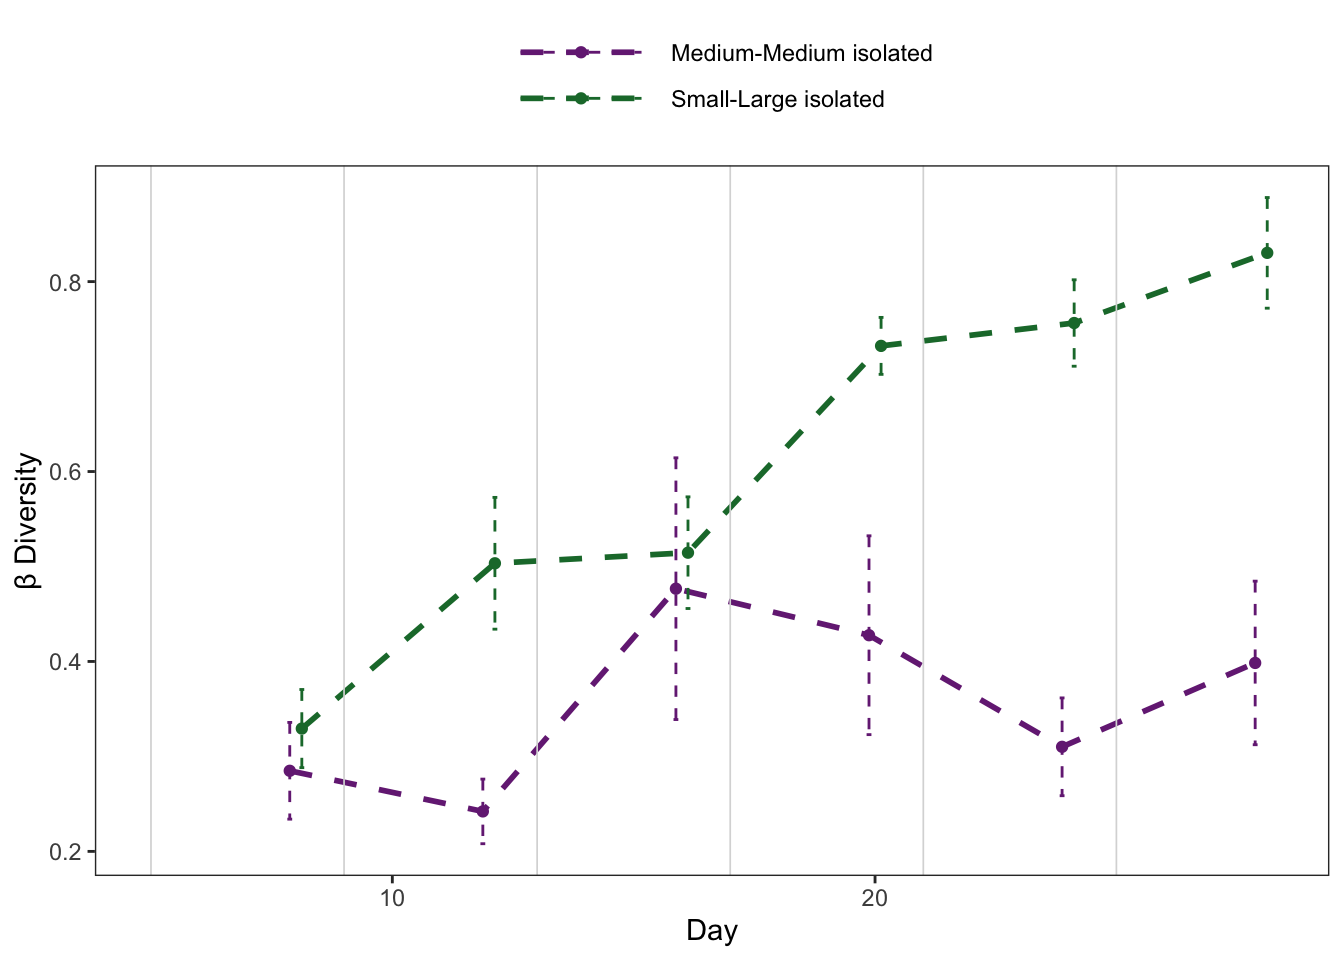
\includegraphics{index_files/figure-latex/unnamed-chunk-171-1.pdf}

\begin{Shaded}
\begin{Highlighting}[]
\FunctionTok{hist}\NormalTok{(iterated\_results\_table}\SpecialCharTok{$}\NormalTok{p\_full, }\AttributeTok{main =} \StringTok{"Distribution of p{-}values of the full model."}\NormalTok{) }
\end{Highlighting}
\end{Shaded}

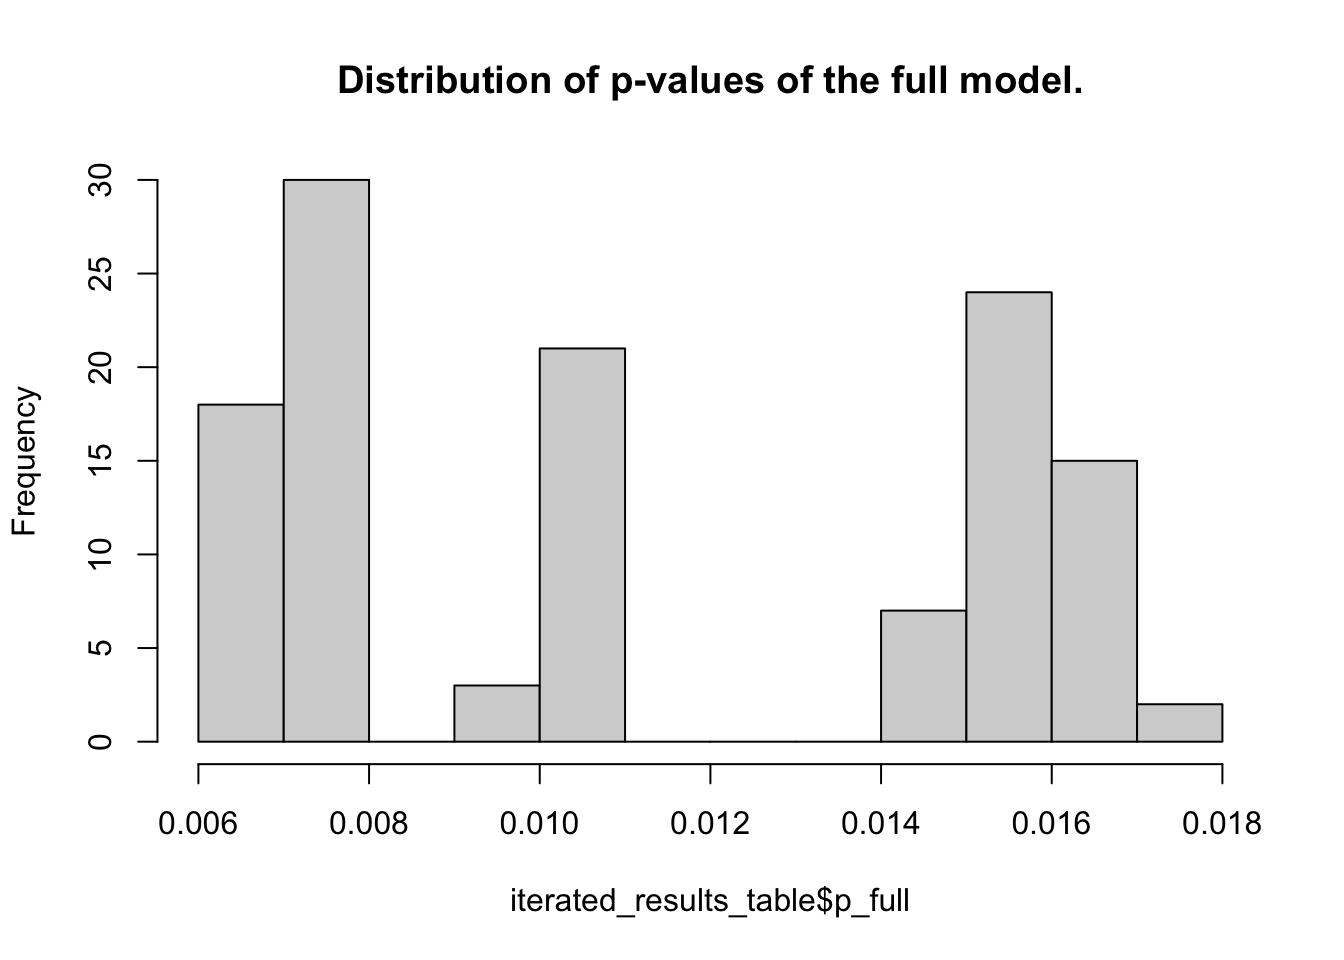
\includegraphics{index_files/figure-latex/unnamed-chunk-171-2.pdf}

\begin{Shaded}
\begin{Highlighting}[]
\FunctionTok{hist}\NormalTok{(iterated\_results\_table}\SpecialCharTok{$}\NormalTok{ΔAIC\_fix, }\AttributeTok{main =} \StringTok{"Distribution of ΔAIC of the fixed model."}\NormalTok{) }
\end{Highlighting}
\end{Shaded}

\begin{verbatim}
## Warning in title(main = main, sub = sub, xlab = xlab, ylab = ylab, ...):
## conversion failure on 'Distribution of ΔAIC of the fixed model.' in
## 'mbcsToSbcs': dot substituted for <ce>
\end{verbatim}

\begin{verbatim}
## Warning in title(main = main, sub = sub, xlab = xlab, ylab = ylab, ...):
## conversion failure on 'Distribution of ΔAIC of the fixed model.' in
## 'mbcsToSbcs': dot substituted for <94>
\end{verbatim}

\begin{verbatim}
## Warning in title(main = main, sub = sub, xlab = xlab, ylab = ylab, ...):
## conversion failure on 'iterated_results_table$ΔAIC_fix' in 'mbcsToSbcs': dot
## substituted for <ce>
\end{verbatim}

\begin{verbatim}
## Warning in title(main = main, sub = sub, xlab = xlab, ylab = ylab, ...):
## conversion failure on 'iterated_results_table$ΔAIC_fix' in 'mbcsToSbcs': dot
## substituted for <94>
\end{verbatim}

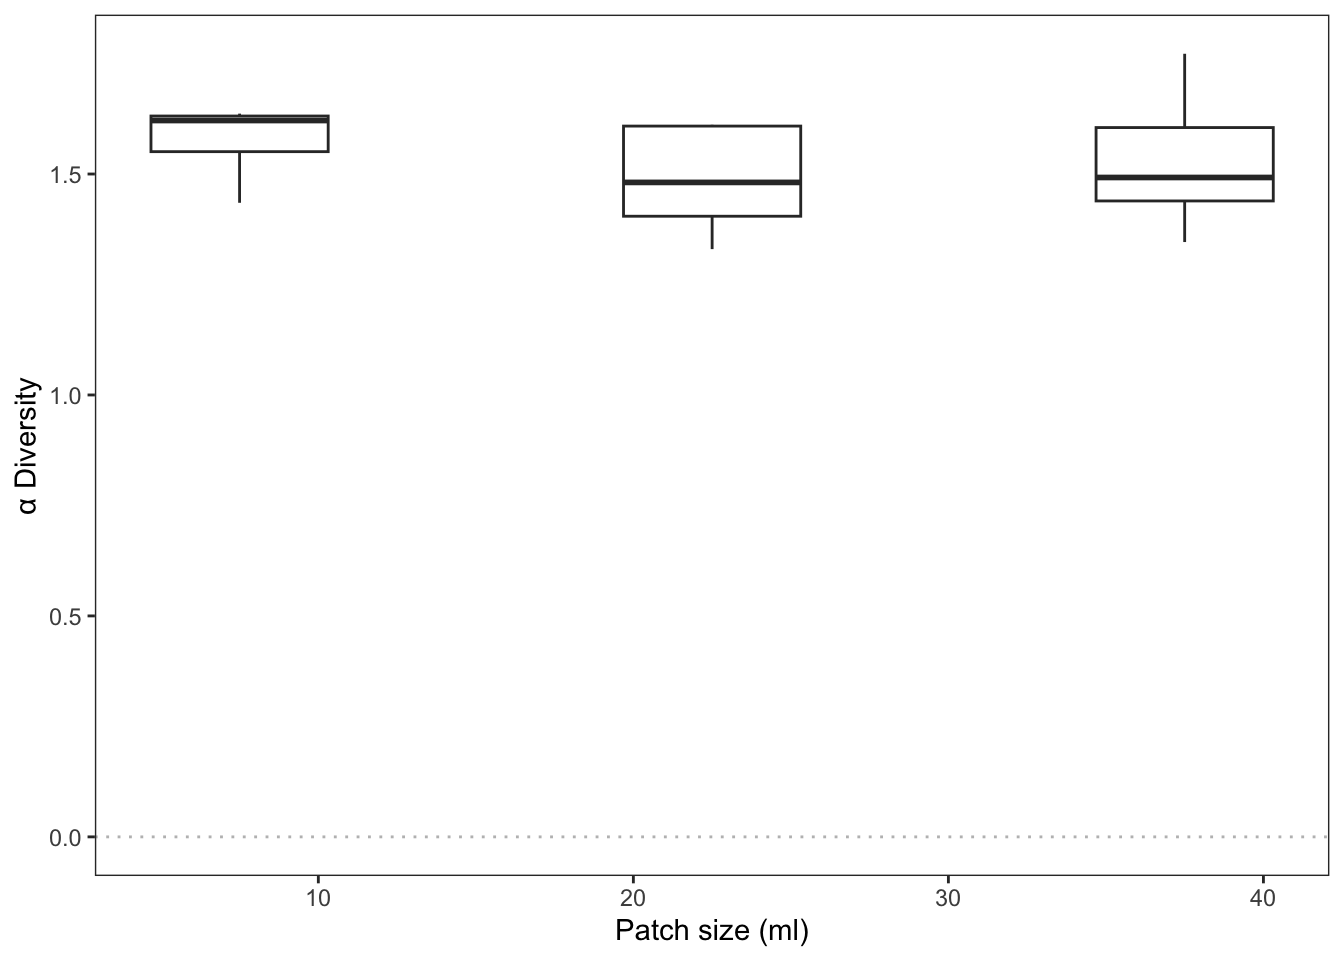
\includegraphics{index_files/figure-latex/unnamed-chunk-171-3.pdf}

\begin{Shaded}
\begin{Highlighting}[]
\FunctionTok{hist}\NormalTok{(iterated\_results\_table}\SpecialCharTok{$}\NormalTok{p\_fix, }\AttributeTok{main =} \StringTok{"Distribution of p{-}values of the fixed model."}\NormalTok{) }
\end{Highlighting}
\end{Shaded}

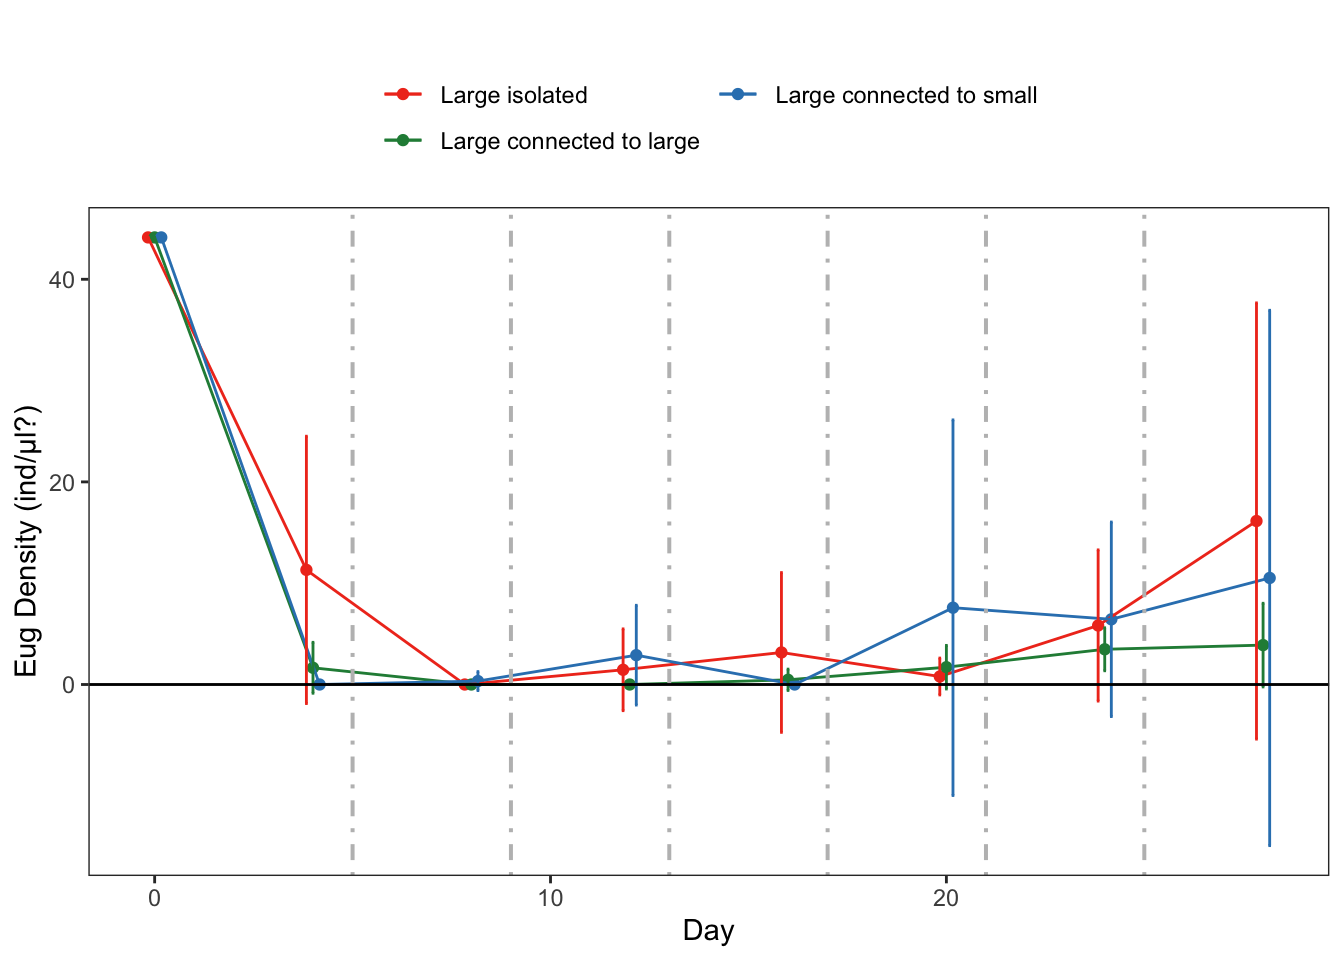
\includegraphics{index_files/figure-latex/unnamed-chunk-171-4.pdf}

\begin{Shaded}
\begin{Highlighting}[]
\FunctionTok{hist}\NormalTok{(iterated\_results\_table}\SpecialCharTok{$}\NormalTok{ΔAIC\_int, }\AttributeTok{main =} \StringTok{"Distribution of ΔAIC of the interation model."}\NormalTok{) }
\end{Highlighting}
\end{Shaded}

\begin{verbatim}
## Warning in title(main = main, sub = sub, xlab = xlab, ylab = ylab, ...):
## conversion failure on 'Distribution of ΔAIC of the interation model.' in
## 'mbcsToSbcs': dot substituted for <ce>
\end{verbatim}

\begin{verbatim}
## Warning in title(main = main, sub = sub, xlab = xlab, ylab = ylab, ...):
## conversion failure on 'Distribution of ΔAIC of the interation model.' in
## 'mbcsToSbcs': dot substituted for <94>
\end{verbatim}

\begin{verbatim}
## Warning in title(main = main, sub = sub, xlab = xlab, ylab = ylab, ...):
## conversion failure on 'iterated_results_table$ΔAIC_int' in 'mbcsToSbcs': dot
## substituted for <ce>
\end{verbatim}

\begin{verbatim}
## Warning in title(main = main, sub = sub, xlab = xlab, ylab = ylab, ...):
## conversion failure on 'iterated_results_table$ΔAIC_int' in 'mbcsToSbcs': dot
## substituted for <94>
\end{verbatim}

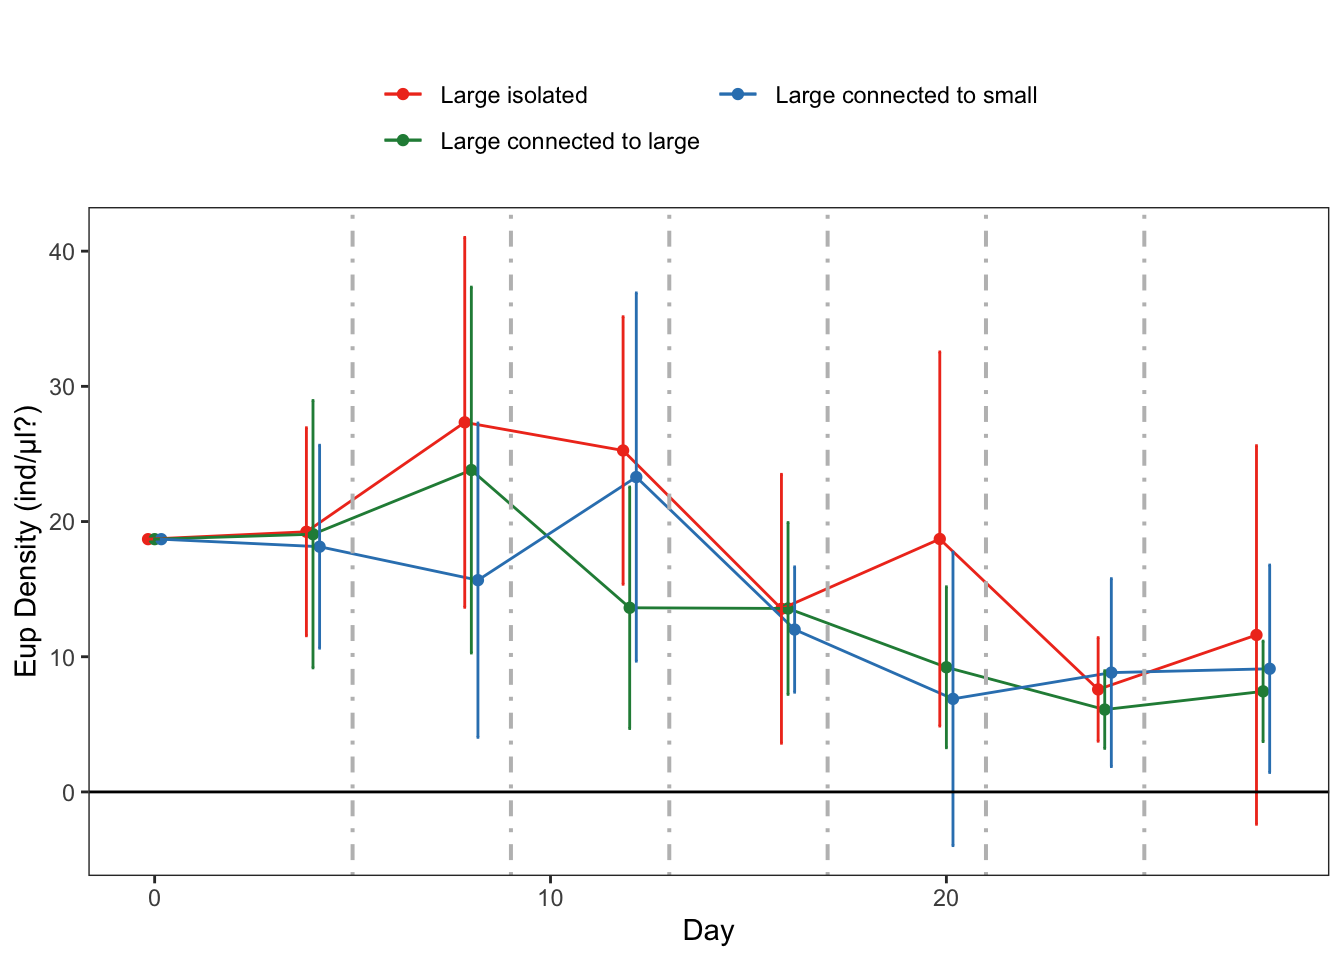
\includegraphics{index_files/figure-latex/unnamed-chunk-171-5.pdf}

\begin{Shaded}
\begin{Highlighting}[]
\FunctionTok{hist}\NormalTok{(iterated\_results\_table}\SpecialCharTok{$}\NormalTok{p\_int, }\AttributeTok{main =} \StringTok{"Distribution of p{-}values of the interation model."}\NormalTok{) }
\end{Highlighting}
\end{Shaded}

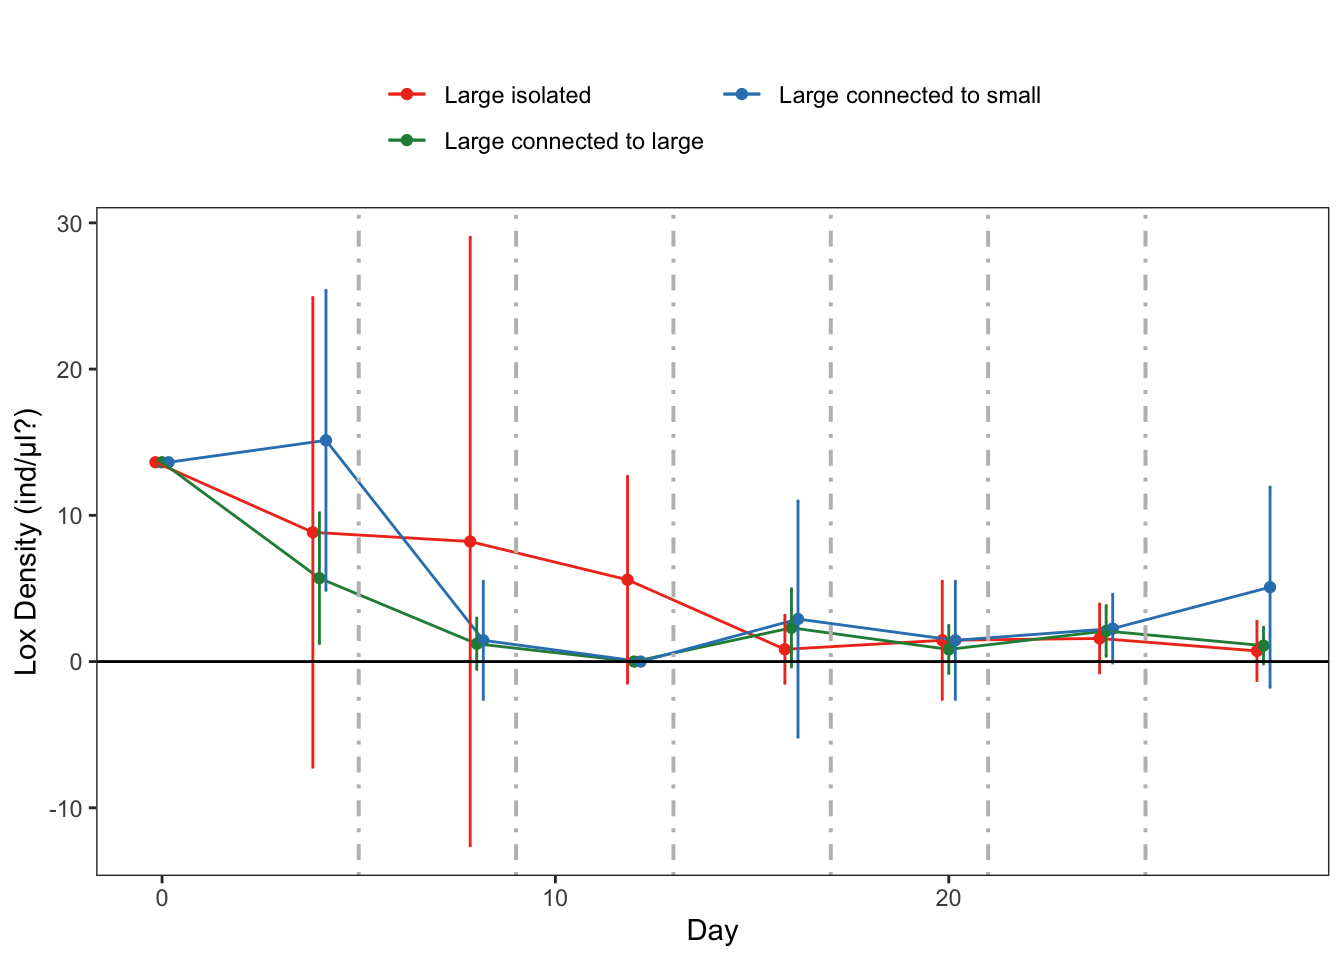
\includegraphics{index_files/figure-latex/unnamed-chunk-171-6.pdf}

\begin{Shaded}
\begin{Highlighting}[]
\CommentTok{\#Use the mean p{-}values and ΔAIC }
\NormalTok{model\_stats\_full }\OtherTok{=} \FunctionTok{data.frame}\NormalTok{(}
  \AttributeTok{deltaAIC =} \FunctionTok{mean}\NormalTok{(iterated\_results\_table}\SpecialCharTok{$}\NormalTok{ΔAIC\_full),}
  \AttributeTok{p\_value =} \FunctionTok{mean}\NormalTok{(iterated\_results\_table}\SpecialCharTok{$}\NormalTok{p\_full),}
  \AttributeTok{R2 =} \ConstantTok{NA}
\NormalTok{) }

\NormalTok{model\_stats\_interaction }\OtherTok{=} \FunctionTok{data.frame}\NormalTok{(}
  \AttributeTok{deltaAIC =} \FunctionTok{mean}\NormalTok{(iterated\_results\_table}\SpecialCharTok{$}\NormalTok{ΔAIC\_int),}
  \AttributeTok{p\_value =} \FunctionTok{mean}\NormalTok{(iterated\_results\_table}\SpecialCharTok{$}\NormalTok{p\_int),}
  \AttributeTok{R2 =} \ConstantTok{NA}
\NormalTok{)}

\NormalTok{model\_stats\_fixed }\OtherTok{=} \FunctionTok{data.frame}\NormalTok{(}
  \AttributeTok{deltaAIC =} \FunctionTok{mean}\NormalTok{(iterated\_results\_table}\SpecialCharTok{$}\NormalTok{ΔAIC\_fix),}
  \AttributeTok{p\_value =} \FunctionTok{mean}\NormalTok{(iterated\_results\_table}\SpecialCharTok{$}\NormalTok{p\_fix),}
  \AttributeTok{R2 =} \ConstantTok{NA}
\NormalTok{)}

\NormalTok{results\_table }\OtherTok{=} \FunctionTok{fill.results.table}\NormalTok{(}
\NormalTok{    results\_table,}
\NormalTok{    response\_variable,}
\NormalTok{    metaecosystem\_type\_input\_model,}
\NormalTok{    model\_stats\_full,}
\NormalTok{    model\_stats\_interaction,}
\NormalTok{    model\_stats\_fixed}
\NormalTok{  )}
\end{Highlighting}
\end{Shaded}

\hypertarget{boxplots-4}{%
\subparagraph{Boxplots}\label{boxplots-4}}

\begin{Shaded}
\begin{Highlighting}[]
\FunctionTok{plot.metaecos.boxplots}\NormalTok{(ds\_metaecosystems,}
\NormalTok{                       metaecosystem\_type\_input,}
\NormalTok{                       response\_variable)}
\end{Highlighting}
\end{Shaded}

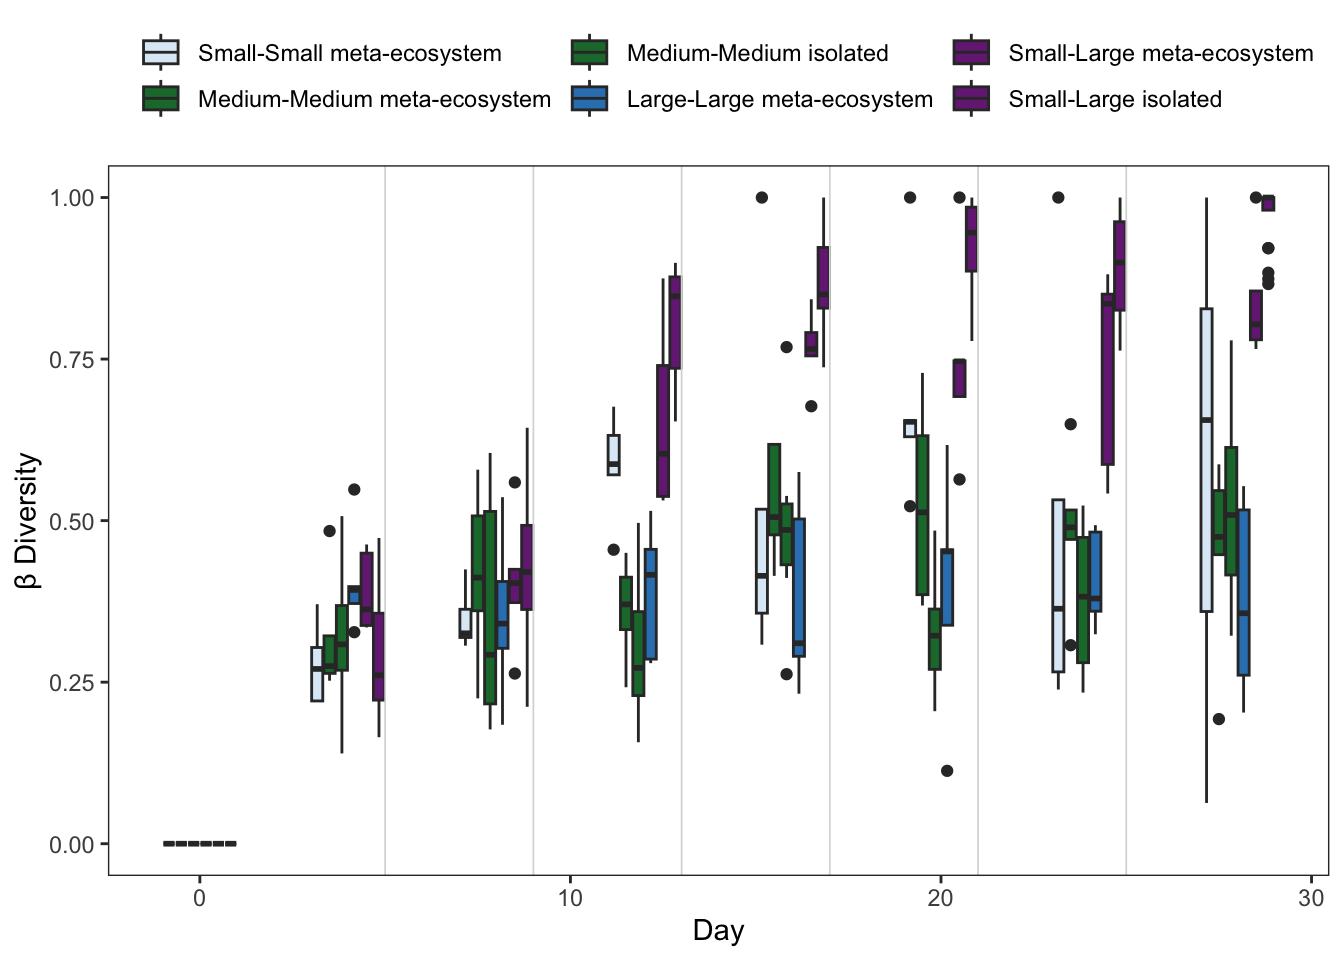
\includegraphics{index_files/figure-latex/unnamed-chunk-159-1.pdf}

\hypertarget{shannon-1}{%
\paragraph{Shannon}\label{shannon-1}}

\begin{Shaded}
\begin{Highlighting}[]
\NormalTok{response\_variable }\OtherTok{=} \StringTok{"mean\_shannon"}
\end{Highlighting}
\end{Shaded}

\hypertarget{means-5}{%
\subparagraph{Means}\label{means-5}}

\begin{Shaded}
\begin{Highlighting}[]
\NormalTok{p\_MM\_SL\_metaecos\_alpha }\OtherTok{=} \FunctionTok{plot.metaecos.points}\NormalTok{(ds\_metaecosystems, }
\NormalTok{                                              metaecosystem\_type\_input,}
\NormalTok{                                              response\_variable) }\SpecialCharTok{\%\textgreater{}\%}
  \FunctionTok{print}\NormalTok{()}
\end{Highlighting}
\end{Shaded}

\begin{verbatim}
## Warning in grid.Call(C_textBounds, as.graphicsAnnot(x$label), x$x, x$y, :
## conversion failure on 'α Diversity' in 'mbcsToSbcs': dot substituted for <ce>
\end{verbatim}

\begin{verbatim}
## Warning in grid.Call(C_textBounds, as.graphicsAnnot(x$label), x$x, x$y, :
## conversion failure on 'α Diversity' in 'mbcsToSbcs': dot substituted for <b1>
\end{verbatim}

\begin{verbatim}
## Warning in grid.Call(C_textBounds, as.graphicsAnnot(x$label), x$x, x$y, :
## conversion failure on 'α Diversity' in 'mbcsToSbcs': dot substituted for <ce>
\end{verbatim}

\begin{verbatim}
## Warning in grid.Call(C_textBounds, as.graphicsAnnot(x$label), x$x, x$y, :
## conversion failure on 'α Diversity' in 'mbcsToSbcs': dot substituted for <b1>
\end{verbatim}

\begin{verbatim}
## Warning in grid.Call(C_textBounds, as.graphicsAnnot(x$label), x$x, x$y, :
## conversion failure on 'α Diversity' in 'mbcsToSbcs': dot substituted for <ce>
\end{verbatim}

\begin{verbatim}
## Warning in grid.Call(C_textBounds, as.graphicsAnnot(x$label), x$x, x$y, :
## conversion failure on 'α Diversity' in 'mbcsToSbcs': dot substituted for <b1>
\end{verbatim}

\begin{verbatim}
## Warning in grid.Call(C_textBounds, as.graphicsAnnot(x$label), x$x, x$y, :
## conversion failure on 'α Diversity' in 'mbcsToSbcs': dot substituted for <ce>
\end{verbatim}

\begin{verbatim}
## Warning in grid.Call(C_textBounds, as.graphicsAnnot(x$label), x$x, x$y, :
## conversion failure on 'α Diversity' in 'mbcsToSbcs': dot substituted for <b1>
\end{verbatim}

\begin{verbatim}
## Warning in grid.Call(C_textBounds, as.graphicsAnnot(x$label), x$x, x$y, :
## conversion failure on 'α Diversity' in 'mbcsToSbcs': dot substituted for <ce>
\end{verbatim}

\begin{verbatim}
## Warning in grid.Call(C_textBounds, as.graphicsAnnot(x$label), x$x, x$y, :
## conversion failure on 'α Diversity' in 'mbcsToSbcs': dot substituted for <b1>
\end{verbatim}

\begin{verbatim}
## Warning in grid.Call(C_textBounds, as.graphicsAnnot(x$label), x$x, x$y, :
## conversion failure on 'α Diversity' in 'mbcsToSbcs': dot substituted for <ce>
\end{verbatim}

\begin{verbatim}
## Warning in grid.Call(C_textBounds, as.graphicsAnnot(x$label), x$x, x$y, :
## conversion failure on 'α Diversity' in 'mbcsToSbcs': dot substituted for <b1>
\end{verbatim}

\begin{verbatim}
## Warning in grid.Call(C_textBounds, as.graphicsAnnot(x$label), x$x, x$y, :
## conversion failure on 'α Diversity' in 'mbcsToSbcs': dot substituted for <ce>
\end{verbatim}

\begin{verbatim}
## Warning in grid.Call(C_textBounds, as.graphicsAnnot(x$label), x$x, x$y, :
## conversion failure on 'α Diversity' in 'mbcsToSbcs': dot substituted for <b1>
\end{verbatim}

\begin{verbatim}
## Warning in grid.Call.graphics(C_text, as.graphicsAnnot(x$label), x$x, x$y, :
## conversion failure on 'α Diversity' in 'mbcsToSbcs': dot substituted for <ce>
\end{verbatim}

\begin{verbatim}
## Warning in grid.Call.graphics(C_text, as.graphicsAnnot(x$label), x$x, x$y, :
## conversion failure on 'α Diversity' in 'mbcsToSbcs': dot substituted for <b1>
\end{verbatim}

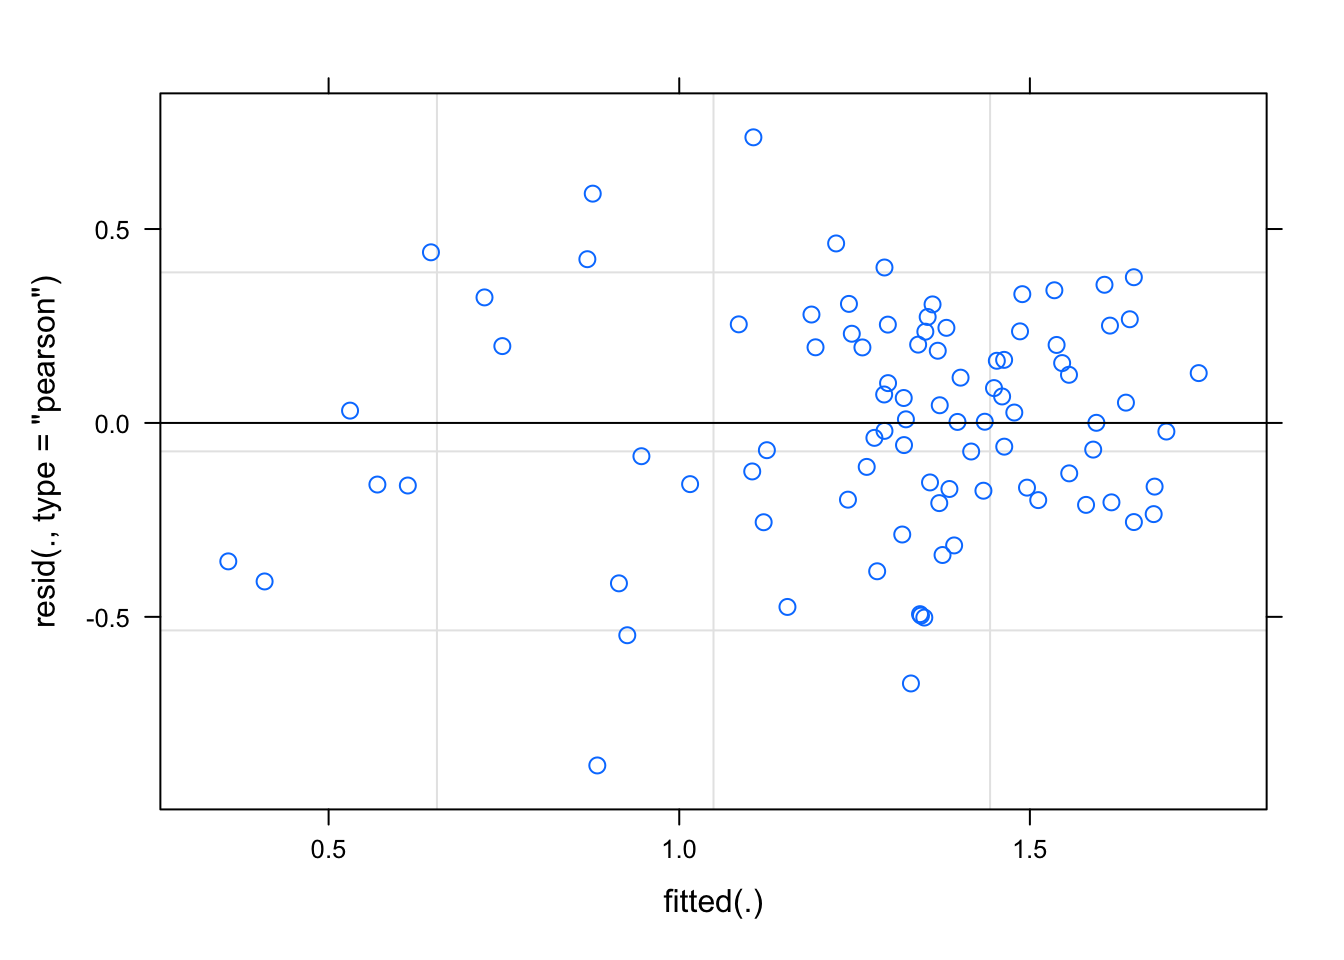
\includegraphics{index_files/figure-latex/unnamed-chunk-174-1.pdf}

Small-Large vs Medium-Medium meta-ecosystems

\begin{Shaded}
\begin{Highlighting}[]
\NormalTok{metaecosystem\_type\_input\_model }\OtherTok{=} \FunctionTok{c}\NormalTok{(}\StringTok{"Small{-}Large meta{-}ecosystem"}\NormalTok{,}
                                   \StringTok{"Medium{-}Medium meta{-}ecosystem"}\NormalTok{)}
\end{Highlighting}
\end{Shaded}

\begin{Shaded}
\begin{Highlighting}[]
\NormalTok{filtered\_data }\OtherTok{=}\NormalTok{ ds\_metaecosystems }\SpecialCharTok{\%\textgreater{}\%}
                         \FunctionTok{filter}\NormalTok{(time\_point }\SpecialCharTok{\textgreater{}=}\NormalTok{ first\_time\_point\_model,}
\NormalTok{                                time\_point }\SpecialCharTok{\textless{}=}\NormalTok{ last\_time\_point\_model,}
\NormalTok{                                metaecosystem\_type }\SpecialCharTok{\%in\%}\NormalTok{ metaecosystem\_type\_input\_model)}
\end{Highlighting}
\end{Shaded}

\begin{Shaded}
\begin{Highlighting}[]
\FunctionTok{plot.metaecos.points}\NormalTok{(filtered\_data,}
\NormalTok{                     metaecosystem\_type\_input\_model,}
\NormalTok{                     response\_variable)}
\end{Highlighting}
\end{Shaded}

\begin{verbatim}
## Warning in grid.Call(C_textBounds, as.graphicsAnnot(x$label), x$x, x$y, :
## conversion failure on 'α Diversity' in 'mbcsToSbcs': dot substituted for <ce>
\end{verbatim}

\begin{verbatim}
## Warning in grid.Call(C_textBounds, as.graphicsAnnot(x$label), x$x, x$y, :
## conversion failure on 'α Diversity' in 'mbcsToSbcs': dot substituted for <b1>
\end{verbatim}

\begin{verbatim}
## Warning in grid.Call(C_textBounds, as.graphicsAnnot(x$label), x$x, x$y, :
## conversion failure on 'α Diversity' in 'mbcsToSbcs': dot substituted for <ce>
\end{verbatim}

\begin{verbatim}
## Warning in grid.Call(C_textBounds, as.graphicsAnnot(x$label), x$x, x$y, :
## conversion failure on 'α Diversity' in 'mbcsToSbcs': dot substituted for <b1>
\end{verbatim}

\begin{verbatim}
## Warning in grid.Call(C_textBounds, as.graphicsAnnot(x$label), x$x, x$y, :
## conversion failure on 'α Diversity' in 'mbcsToSbcs': dot substituted for <ce>
\end{verbatim}

\begin{verbatim}
## Warning in grid.Call(C_textBounds, as.graphicsAnnot(x$label), x$x, x$y, :
## conversion failure on 'α Diversity' in 'mbcsToSbcs': dot substituted for <b1>
\end{verbatim}

\begin{verbatim}
## Warning in grid.Call(C_textBounds, as.graphicsAnnot(x$label), x$x, x$y, :
## conversion failure on 'α Diversity' in 'mbcsToSbcs': dot substituted for <ce>
\end{verbatim}

\begin{verbatim}
## Warning in grid.Call(C_textBounds, as.graphicsAnnot(x$label), x$x, x$y, :
## conversion failure on 'α Diversity' in 'mbcsToSbcs': dot substituted for <b1>
\end{verbatim}

\begin{verbatim}
## Warning in grid.Call(C_textBounds, as.graphicsAnnot(x$label), x$x, x$y, :
## conversion failure on 'α Diversity' in 'mbcsToSbcs': dot substituted for <ce>
\end{verbatim}

\begin{verbatim}
## Warning in grid.Call(C_textBounds, as.graphicsAnnot(x$label), x$x, x$y, :
## conversion failure on 'α Diversity' in 'mbcsToSbcs': dot substituted for <b1>
\end{verbatim}

\begin{verbatim}
## Warning in grid.Call(C_textBounds, as.graphicsAnnot(x$label), x$x, x$y, :
## conversion failure on 'α Diversity' in 'mbcsToSbcs': dot substituted for <ce>
\end{verbatim}

\begin{verbatim}
## Warning in grid.Call(C_textBounds, as.graphicsAnnot(x$label), x$x, x$y, :
## conversion failure on 'α Diversity' in 'mbcsToSbcs': dot substituted for <b1>
\end{verbatim}

\begin{verbatim}
## Warning in grid.Call(C_textBounds, as.graphicsAnnot(x$label), x$x, x$y, :
## conversion failure on 'α Diversity' in 'mbcsToSbcs': dot substituted for <ce>
\end{verbatim}

\begin{verbatim}
## Warning in grid.Call(C_textBounds, as.graphicsAnnot(x$label), x$x, x$y, :
## conversion failure on 'α Diversity' in 'mbcsToSbcs': dot substituted for <b1>
\end{verbatim}

\begin{verbatim}
## Warning in grid.Call.graphics(C_text, as.graphicsAnnot(x$label), x$x, x$y, :
## conversion failure on 'α Diversity' in 'mbcsToSbcs': dot substituted for <ce>
\end{verbatim}

\begin{verbatim}
## Warning in grid.Call.graphics(C_text, as.graphicsAnnot(x$label), x$x, x$y, :
## conversion failure on 'α Diversity' in 'mbcsToSbcs': dot substituted for <b1>
\end{verbatim}

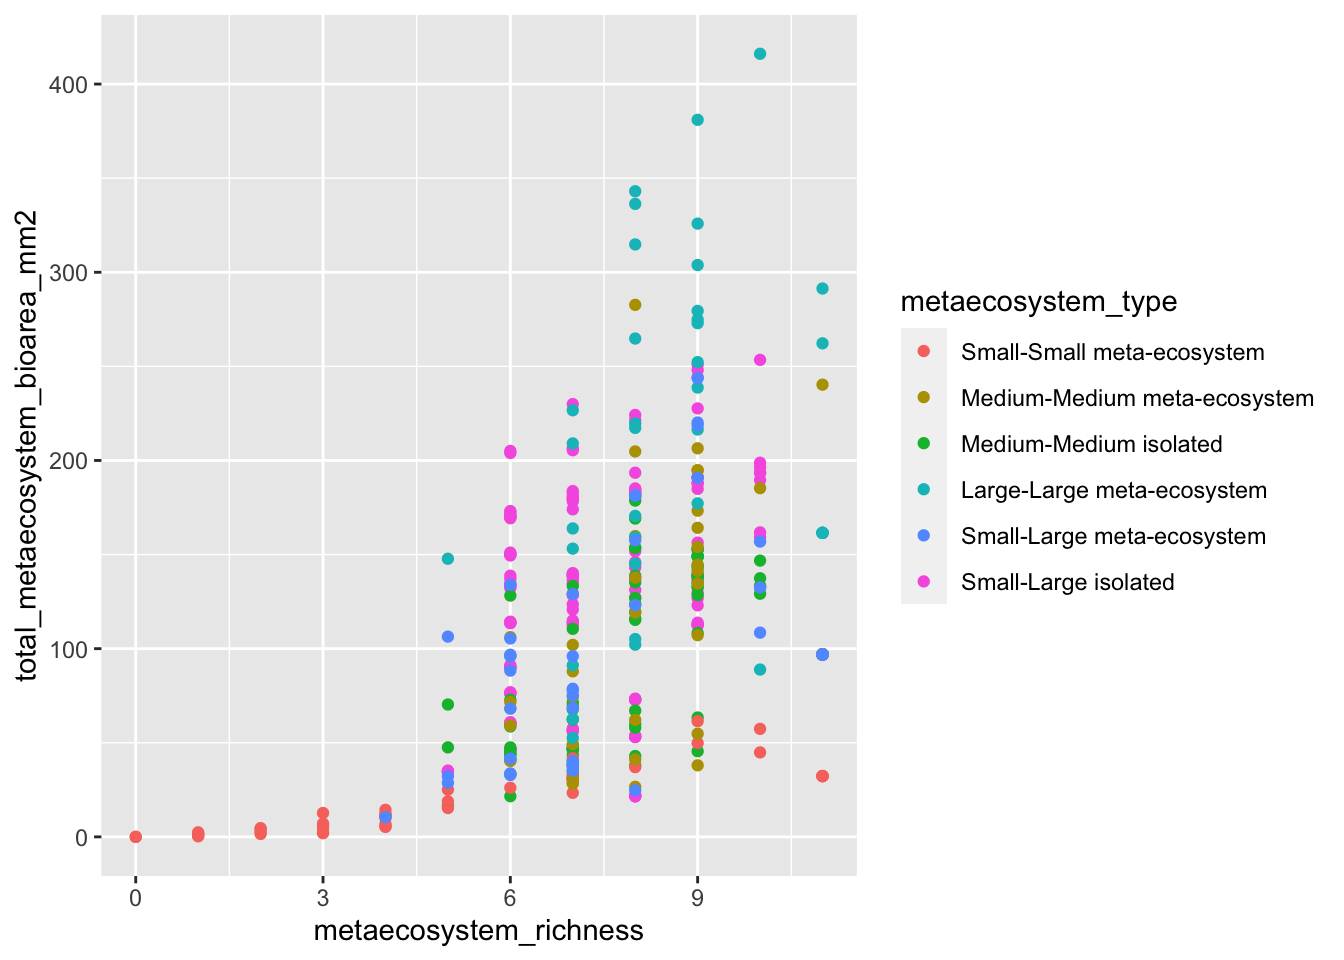
\includegraphics{index_files/figure-latex/unnamed-chunk-183-1.pdf}

\begin{itemize}
\tightlist
\item
  Null model
\end{itemize}

\begin{Shaded}
\begin{Highlighting}[]
\NormalTok{null\_model }\OtherTok{=} \FunctionTok{lmer}\NormalTok{(}
  \FunctionTok{get}\NormalTok{(response\_variable) }\SpecialCharTok{\textasciitilde{}}
\NormalTok{    day }\SpecialCharTok{+} 
\NormalTok{    (day }\SpecialCharTok{|}\NormalTok{ system\_nr), }
  \AttributeTok{data =}\NormalTok{ filtered\_data,}
  \AttributeTok{REML =} \ConstantTok{FALSE}\NormalTok{,}
  \AttributeTok{control =} \FunctionTok{lmerControl}\NormalTok{(}\AttributeTok{optimizer =} \StringTok{"Nelder\_Mead"}\NormalTok{)}
\NormalTok{)}

\FunctionTok{summary}\NormalTok{(null\_model)}
\end{Highlighting}
\end{Shaded}

\begin{verbatim}
## Linear mixed model fit by maximum likelihood  ['lmerMod']
## Formula: get(response_variable) ~ day + (day | system_nr)
##    Data: filtered_data
## Control: lmerControl(optimizer = "Nelder_Mead")
## 
##      AIC      BIC   logLik deviance df.resid 
##    -15.1     -2.5     13.5    -27.1       54 
## 
## Scaled residuals: 
##     Min      1Q  Median      3Q     Max 
## -2.3487 -0.4858  0.1143  0.6922  1.9448 
## 
## Random effects:
##  Groups    Name        Variance  Std.Dev. Corr 
##  system_nr (Intercept) 0.0074871 0.08653       
##            day         0.0000013 0.00114  -1.00
##  Residual              0.0338744 0.18405       
## Number of obs: 60, groups:  system_nr, 10
## 
## Fixed effects:
##             Estimate Std. Error t value
## (Intercept) 1.350442   0.072340  18.668
## day         0.001142   0.003497   0.326
## 
## Correlation of Fixed Effects:
##     (Intr)
## day -0.900
## optimizer (Nelder_Mead) convergence code: 0 (OK)
## boundary (singular) fit: see help('isSingular')
\end{verbatim}

\begin{Shaded}
\begin{Highlighting}[]
\FunctionTok{plot}\NormalTok{(null\_model)}
\end{Highlighting}
\end{Shaded}

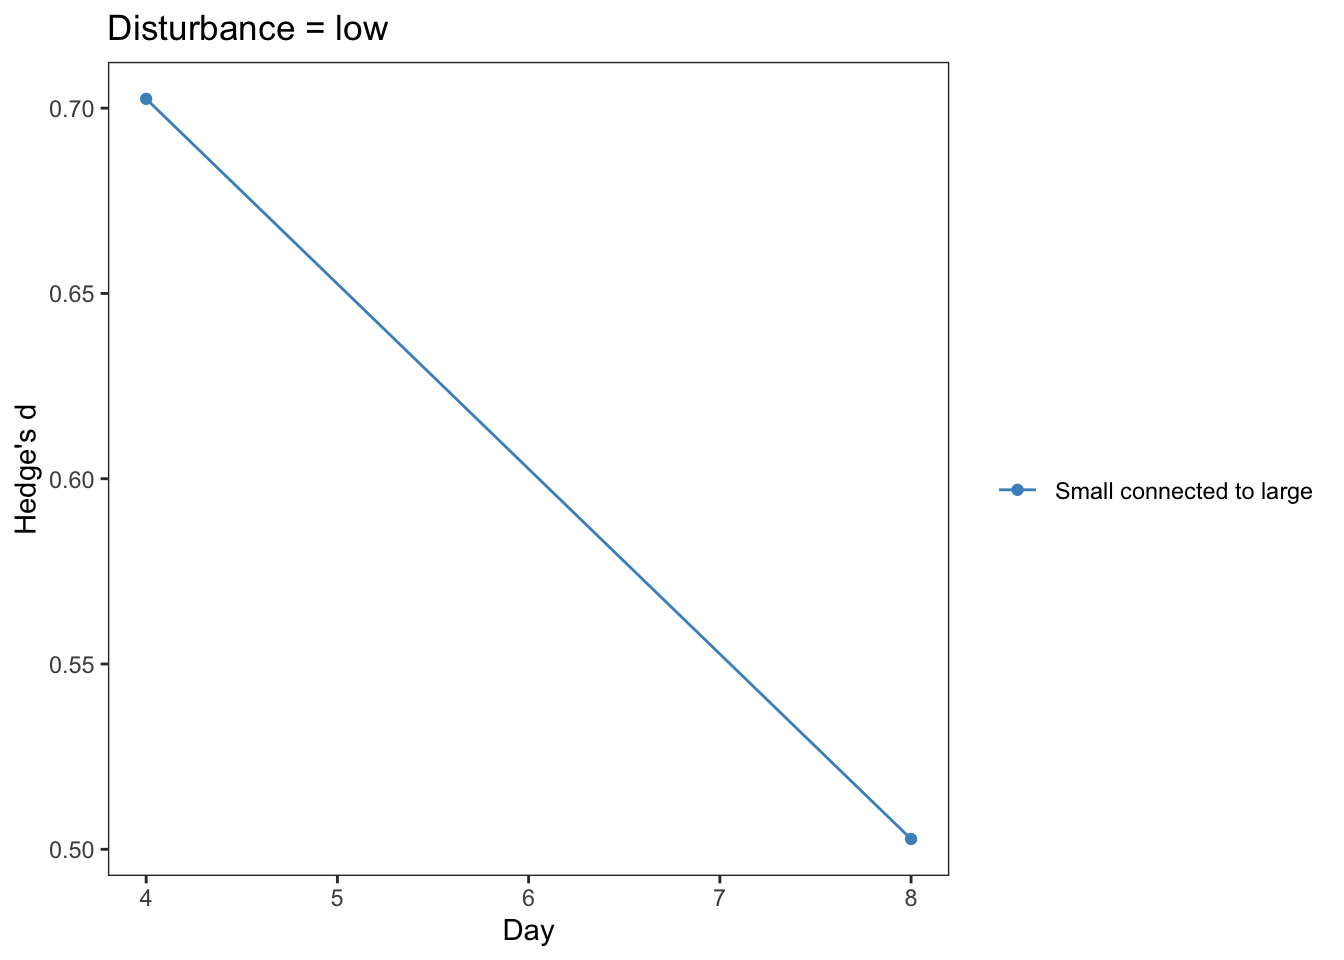
\includegraphics{index_files/figure-latex/unnamed-chunk-184-1.pdf}

\begin{Shaded}
\begin{Highlighting}[]
\FunctionTok{qqnorm}\NormalTok{(}\FunctionTok{resid}\NormalTok{(null\_model))}
\end{Highlighting}
\end{Shaded}

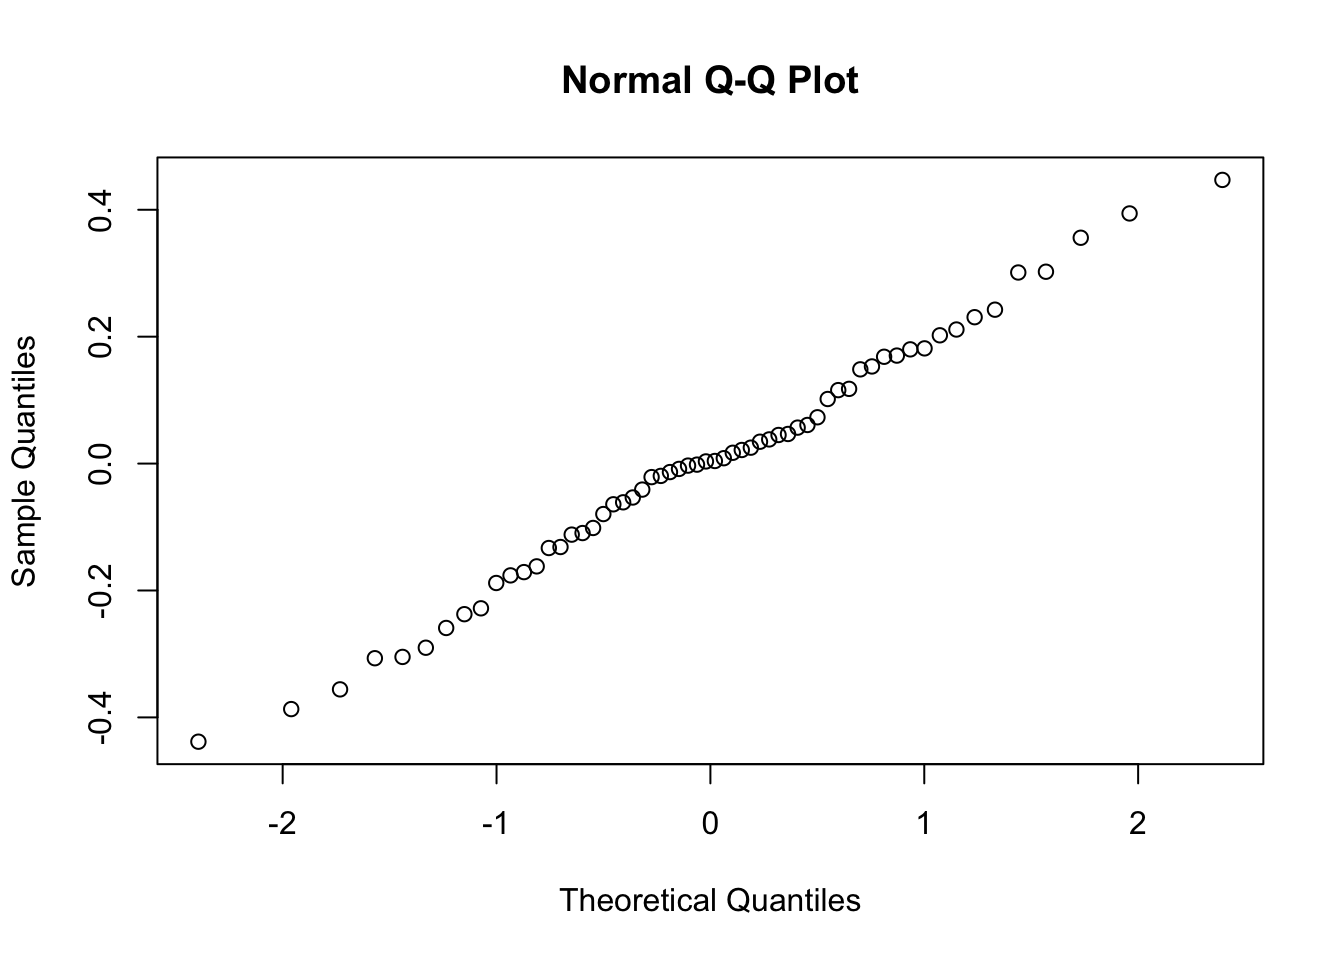
\includegraphics{index_files/figure-latex/unnamed-chunk-184-2.pdf}

\begin{itemize}
\tightlist
\item
  Full model (with \texttt{patch\_size\_symmetry} and
  \texttt{patch\_size\_symmetry:day})
\end{itemize}

\begin{Shaded}
\begin{Highlighting}[]
\NormalTok{full\_model }\OtherTok{=} \FunctionTok{lmer}\NormalTok{(}
  \FunctionTok{get}\NormalTok{(response\_variable) }\SpecialCharTok{\textasciitilde{}}
\NormalTok{    day }\SpecialCharTok{+} 
\NormalTok{    patch\_size\_symmetry }\SpecialCharTok{+}
\NormalTok{    patch\_size\_symmetry }\SpecialCharTok{:}\NormalTok{ day }\SpecialCharTok{+} 
\NormalTok{    (day }\SpecialCharTok{|}\NormalTok{ system\_nr), }
  \AttributeTok{data =}\NormalTok{ filtered\_data,}
  \AttributeTok{REML =} \ConstantTok{FALSE}\NormalTok{,}
  \AttributeTok{control =} \FunctionTok{lmerControl}\NormalTok{(}\AttributeTok{optimizer =} \StringTok{"Nelder\_Mead"}\NormalTok{)}
\NormalTok{)}

\FunctionTok{summary}\NormalTok{(full\_model)}
\end{Highlighting}
\end{Shaded}

\begin{verbatim}
## Linear mixed model fit by maximum likelihood  ['lmerMod']
## Formula: 
## get(response_variable) ~ day + patch_size_symmetry + patch_size_symmetry:day +  
##     (day | system_nr)
##    Data: filtered_data
## Control: lmerControl(optimizer = "Nelder_Mead")
## 
##      AIC      BIC   logLik deviance df.resid 
##    -12.6      4.2     14.3    -28.6       52 
## 
## Scaled residuals: 
##      Min       1Q   Median       3Q      Max 
## -2.44017 -0.59444  0.09632  0.71275  1.87105 
## 
## Random effects:
##  Groups    Name        Variance  Std.Dev. Corr 
##  system_nr (Intercept) 8.522e-03 0.092316      
##            day         3.258e-06 0.001805 -1.00
##  Residual              3.338e-02 0.182693      
## Number of obs: 60, groups:  system_nr, 10
## 
## Fixed effects:
##                                   Estimate Std. Error t value
## (Intercept)                       1.339689   0.102671  13.048
## day                               0.003439   0.004949   0.695
## patch_size_symmetrysymmetric      0.021505   0.145199   0.148
## day:patch_size_symmetrysymmetric -0.004596   0.006999  -0.657
## 
## Correlation of Fixed Effects:
##             (Intr) day    ptch__
## day         -0.910              
## ptch_sz_sym -0.707  0.644       
## dy:ptch_sz_  0.644 -0.707 -0.910
## optimizer (Nelder_Mead) convergence code: 0 (OK)
## boundary (singular) fit: see help('isSingular')
\end{verbatim}

\begin{Shaded}
\begin{Highlighting}[]
\FunctionTok{plot}\NormalTok{(full\_model)}
\end{Highlighting}
\end{Shaded}

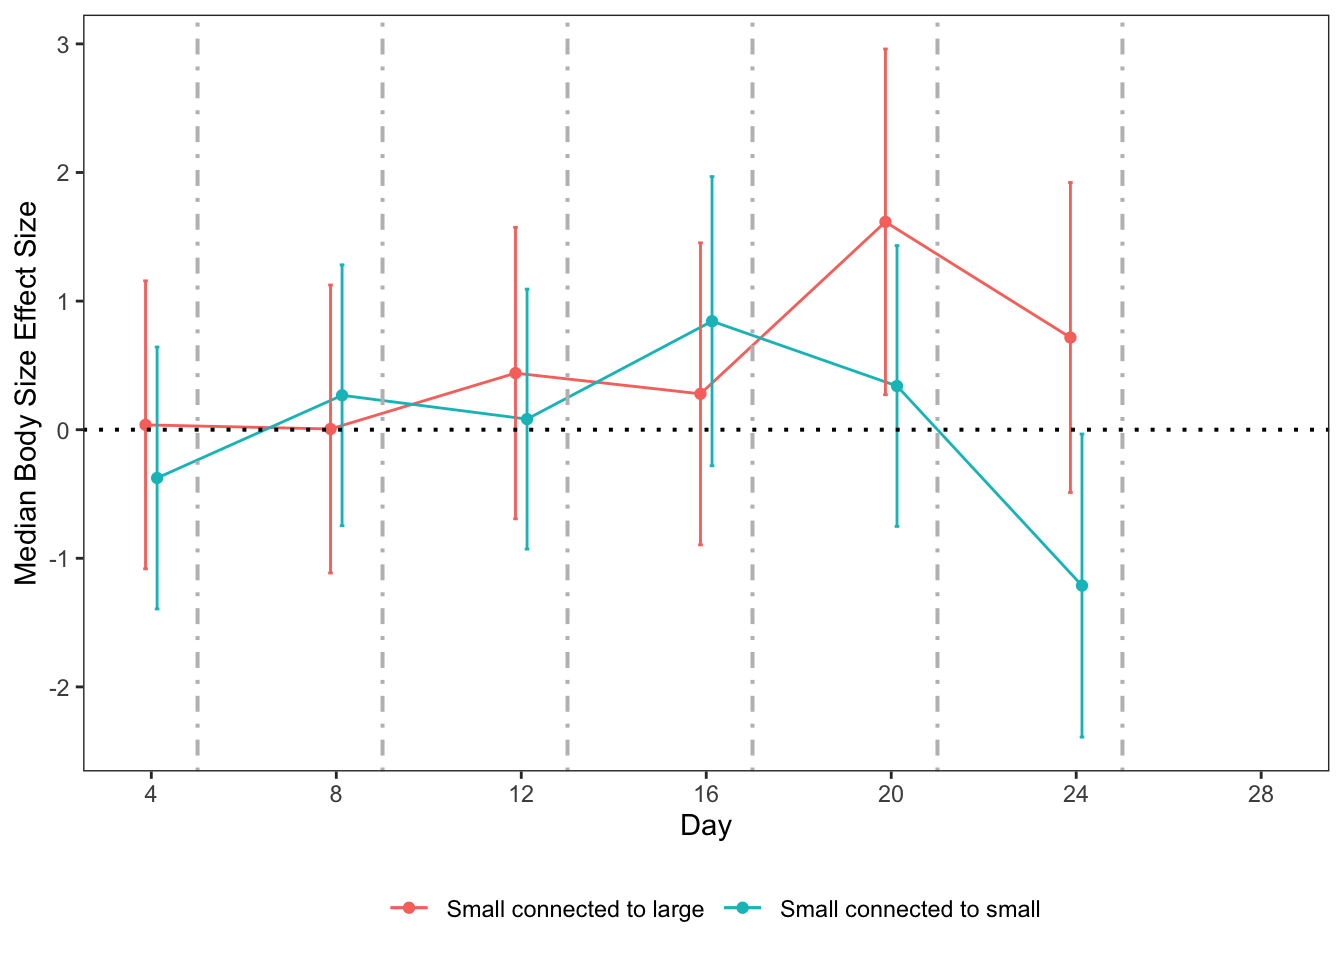
\includegraphics{index_files/figure-latex/unnamed-chunk-185-1.pdf}

\begin{Shaded}
\begin{Highlighting}[]
\FunctionTok{qqnorm}\NormalTok{(}\FunctionTok{resid}\NormalTok{(full\_model))}
\end{Highlighting}
\end{Shaded}

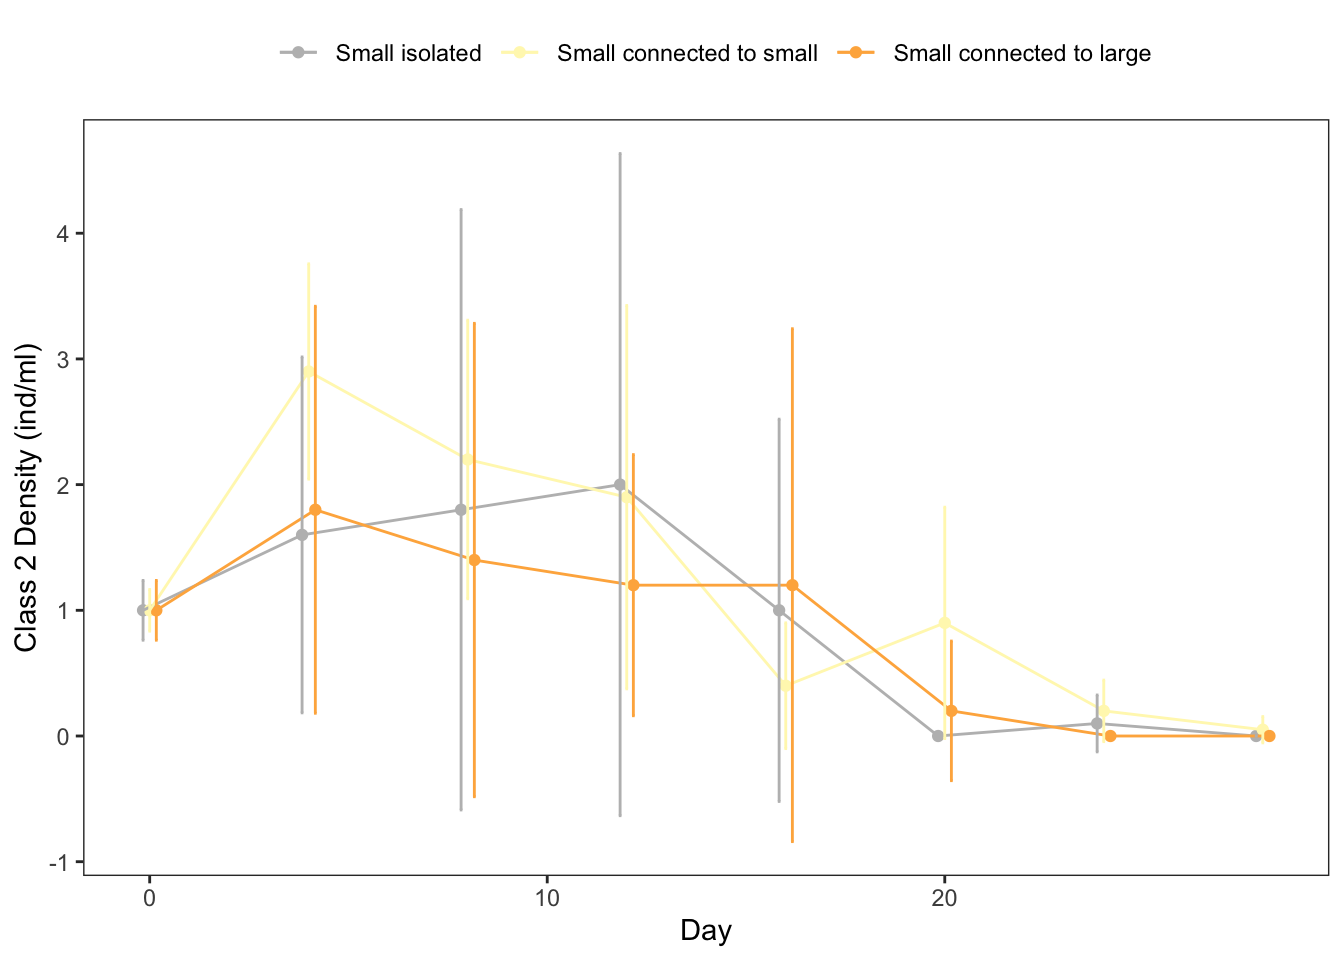
\includegraphics{index_files/figure-latex/unnamed-chunk-185-2.pdf}

\begin{Shaded}
\begin{Highlighting}[]
\NormalTok{model\_stats\_full }\OtherTok{=} \FunctionTok{compute.model.stats}\NormalTok{(full\_model,}
\NormalTok{                                       null\_model,}
                                       \StringTok{"mixed\_model"}\NormalTok{) }\SpecialCharTok{\%\textgreater{}\%}
  \FunctionTok{print}\NormalTok{()}
\end{Highlighting}
\end{Shaded}

\begin{verbatim}
##   deltaAIC  p_value R2
## 1 2.465452 0.464277 NA
\end{verbatim}

\begin{itemize}
\tightlist
\item
  Interaction model (with \texttt{patch\_size\_symmetry:day})
\end{itemize}

\begin{Shaded}
\begin{Highlighting}[]
\NormalTok{interaction\_model }\OtherTok{=} \FunctionTok{lmer}\NormalTok{(}
  \FunctionTok{get}\NormalTok{(response\_variable) }\SpecialCharTok{\textasciitilde{}}
\NormalTok{    day }\SpecialCharTok{+} 
\NormalTok{    patch\_size\_symmetry }\SpecialCharTok{:}\NormalTok{ day }\SpecialCharTok{+} 
\NormalTok{    (day }\SpecialCharTok{|}\NormalTok{ system\_nr), }
  \AttributeTok{data =}\NormalTok{ filtered\_data,}
  \AttributeTok{REML =} \ConstantTok{FALSE}\NormalTok{,}
  \AttributeTok{control =} \FunctionTok{lmerControl}\NormalTok{(}\AttributeTok{optimizer =} \StringTok{"Nelder\_Mead"}\NormalTok{)}
\NormalTok{)}

\FunctionTok{summary}\NormalTok{(interaction\_model)}
\end{Highlighting}
\end{Shaded}

\begin{verbatim}
## Linear mixed model fit by maximum likelihood  ['lmerMod']
## Formula: get(response_variable) ~ day + patch_size_symmetry:day + (day |  
##     system_nr)
##    Data: filtered_data
## Control: lmerControl(optimizer = "Nelder_Mead")
## 
##      AIC      BIC   logLik deviance df.resid 
##    -14.6      0.1     14.3    -28.6       53 
## 
## Scaled residuals: 
##     Min      1Q  Median      3Q     Max 
## -2.4507 -0.6032  0.1008  0.7067  1.8534 
## 
## Random effects:
##  Groups    Name        Variance  Std.Dev. Corr 
##  system_nr (Intercept) 8.571e-03 0.092577      
##            day         3.302e-06 0.001817 -1.00
##  Residual              3.339e-02 0.182717      
## Number of obs: 60, groups:  system_nr, 10
## 
## Fixed effects:
##                                   Estimate Std. Error t value
## (Intercept)                       1.350442   0.072640  18.591
## day                               0.002968   0.003789   0.783
## day:patch_size_symmetrysymmetric -0.003652   0.002900  -1.260
## 
## Correlation of Fixed Effects:
##             (Intr) day   
## day         -0.841       
## dy:ptch_sz_  0.000 -0.383
## optimizer (Nelder_Mead) convergence code: 0 (OK)
## boundary (singular) fit: see help('isSingular')
\end{verbatim}

\begin{Shaded}
\begin{Highlighting}[]
\FunctionTok{plot}\NormalTok{(interaction\_model)}
\end{Highlighting}
\end{Shaded}

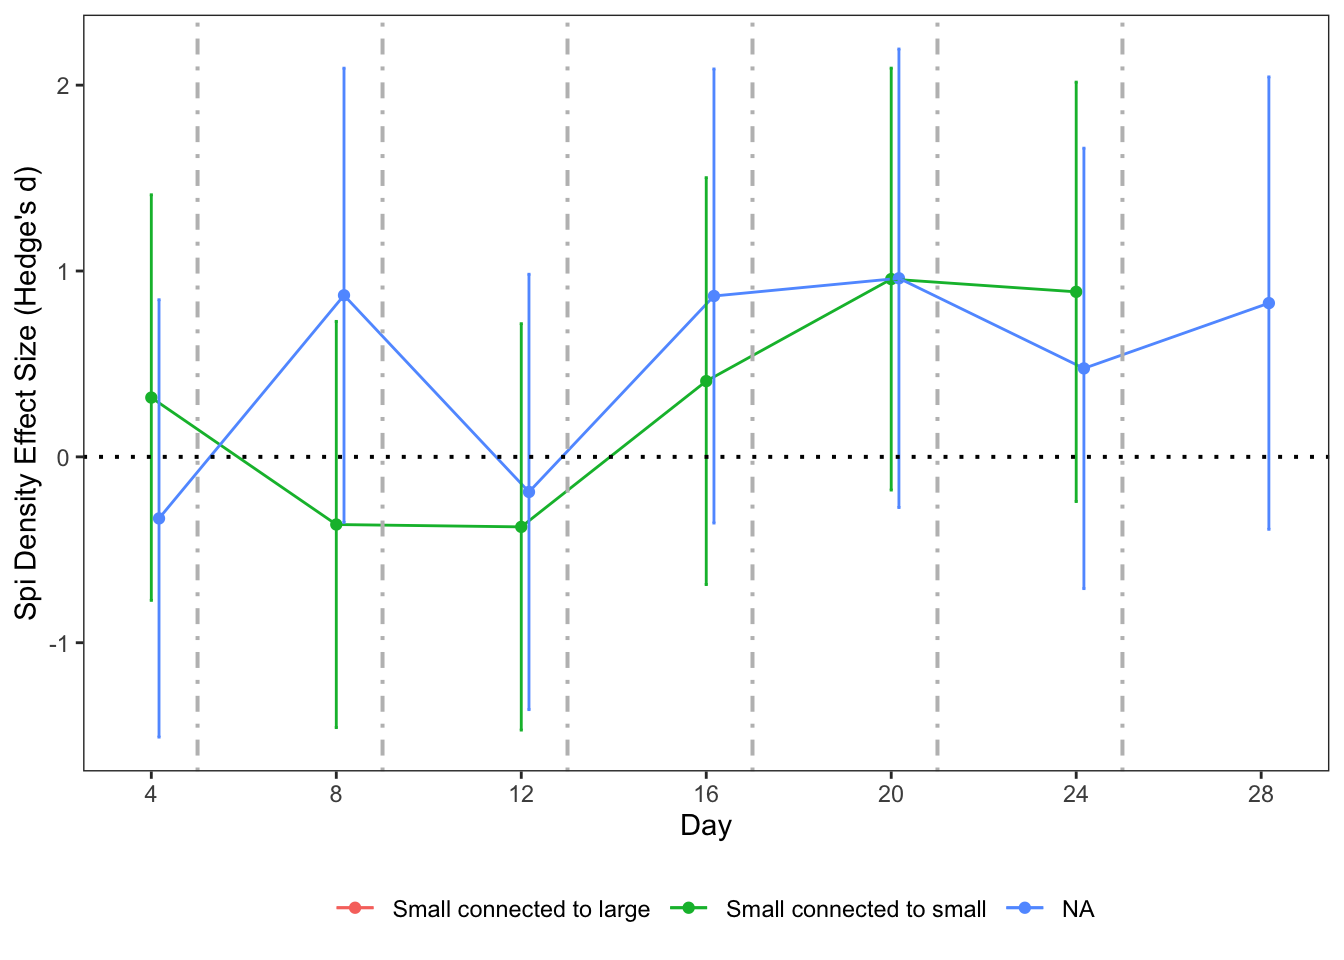
\includegraphics{index_files/figure-latex/unnamed-chunk-186-1.pdf}

\begin{Shaded}
\begin{Highlighting}[]
\FunctionTok{qqnorm}\NormalTok{(}\FunctionTok{resid}\NormalTok{(interaction\_model))}
\end{Highlighting}
\end{Shaded}

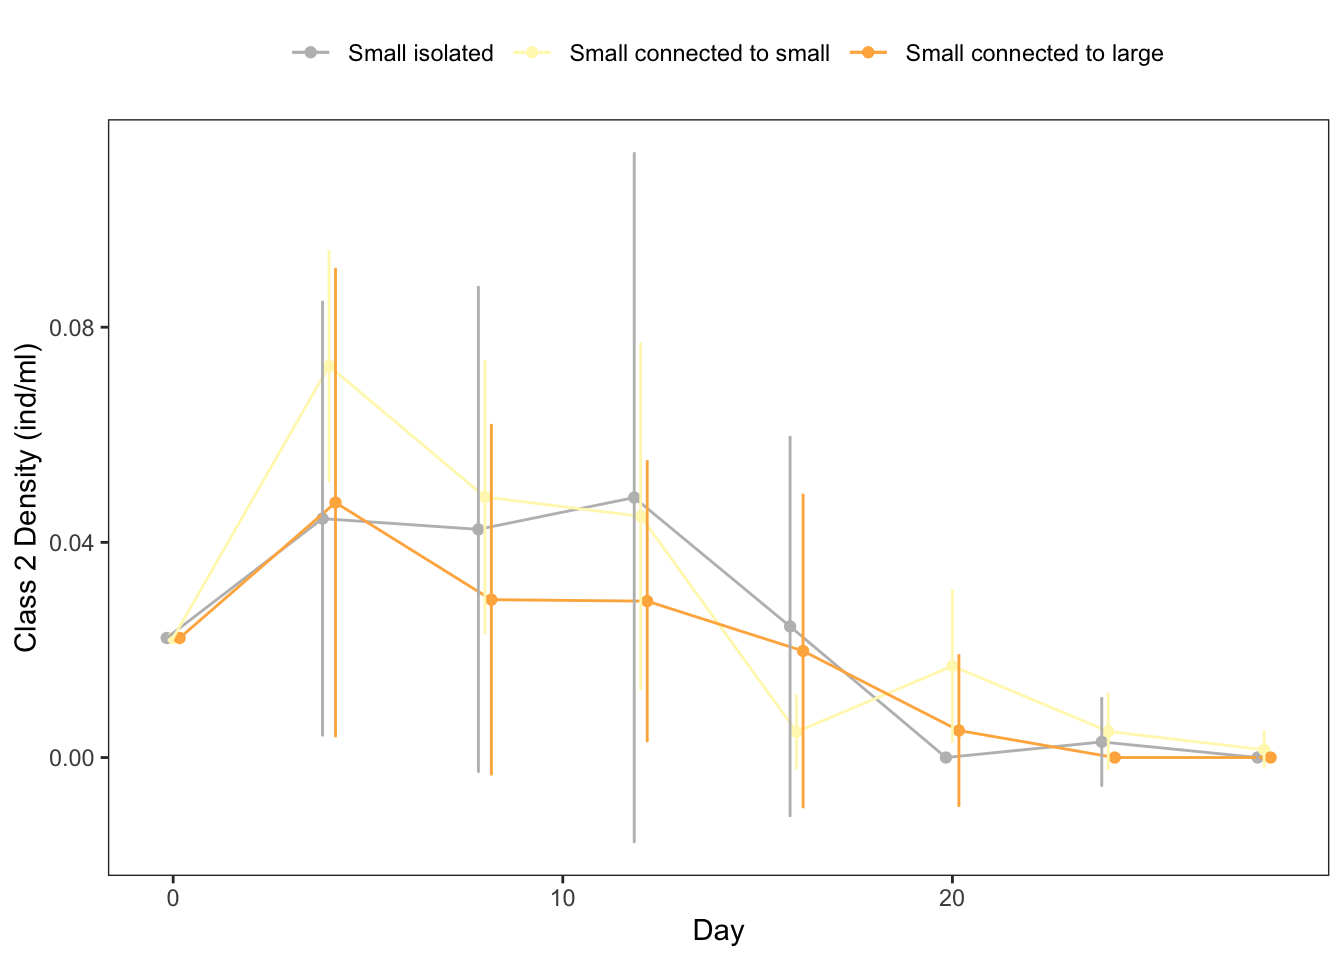
\includegraphics{index_files/figure-latex/unnamed-chunk-186-2.pdf}

\begin{Shaded}
\begin{Highlighting}[]
\NormalTok{model\_stats\_interaction }\OtherTok{=} \FunctionTok{compute.model.stats}\NormalTok{(interaction\_model,}
\NormalTok{                                              null\_model,}
                                              \StringTok{"mixed\_model"}\NormalTok{) }\SpecialCharTok{\%\textgreater{}\%}
  \FunctionTok{print}\NormalTok{()}
\end{Highlighting}
\end{Shaded}

\begin{verbatim}
##    deltaAIC   p_value R2
## 1 0.4873745 0.2187389 NA
\end{verbatim}

\begin{itemize}
\tightlist
\item
  Fixed model (with \texttt{patch\_size\_symmetry})
\end{itemize}

\begin{Shaded}
\begin{Highlighting}[]
\NormalTok{fixed\_model }\OtherTok{=} \FunctionTok{lmer}\NormalTok{(}
  \FunctionTok{get}\NormalTok{(response\_variable) }\SpecialCharTok{\textasciitilde{}}
\NormalTok{    day }\SpecialCharTok{+} 
\NormalTok{    patch\_size\_symmetry }\SpecialCharTok{+} 
\NormalTok{    (day }\SpecialCharTok{|}\NormalTok{ system\_nr), }
  \AttributeTok{data =}\NormalTok{ filtered\_data,}
  \AttributeTok{REML =} \ConstantTok{FALSE}\NormalTok{,}
  \AttributeTok{control =} \FunctionTok{lmerControl}\NormalTok{(}\AttributeTok{optimizer =} \StringTok{"Nelder\_Mead"}\NormalTok{)}
\NormalTok{)}

\FunctionTok{summary}\NormalTok{(fixed\_model)}
\end{Highlighting}
\end{Shaded}

\begin{verbatim}
## Linear mixed model fit by maximum likelihood  ['lmerMod']
## Formula: get(response_variable) ~ day + patch_size_symmetry + (day | system_nr)
##    Data: filtered_data
## Control: lmerControl(optimizer = "Nelder_Mead")
## 
##      AIC      BIC   logLik deviance df.resid 
##    -14.2      0.5     14.1    -28.2       53 
## 
## Scaled residuals: 
##     Min      1Q  Median      3Q     Max 
## -2.4547 -0.5626  0.1031  0.6864  1.8704 
## 
## Random effects:
##  Groups    Name        Variance  Std.Dev. Corr 
##  system_nr (Intercept) 8.824e-03 0.093937      
##            day         3.652e-06 0.001911 -1.00
##  Residual              3.364e-02 0.183422      
## Number of obs: 60, groups:  system_nr, 10
## 
## Fixed effects:
##                               Estimate Std. Error t value
## (Intercept)                   1.383161   0.079000  17.508
## day                           0.001142   0.003519   0.324
## patch_size_symmetrysymmetric -0.065439   0.060159  -1.088
## 
## Correlation of Fixed Effects:
##             (Intr) day   
## day         -0.843       
## ptch_sz_sym -0.381  0.000
## optimizer (Nelder_Mead) convergence code: 0 (OK)
## boundary (singular) fit: see help('isSingular')
\end{verbatim}

\begin{Shaded}
\begin{Highlighting}[]
\FunctionTok{plot}\NormalTok{(fixed\_model)}
\end{Highlighting}
\end{Shaded}

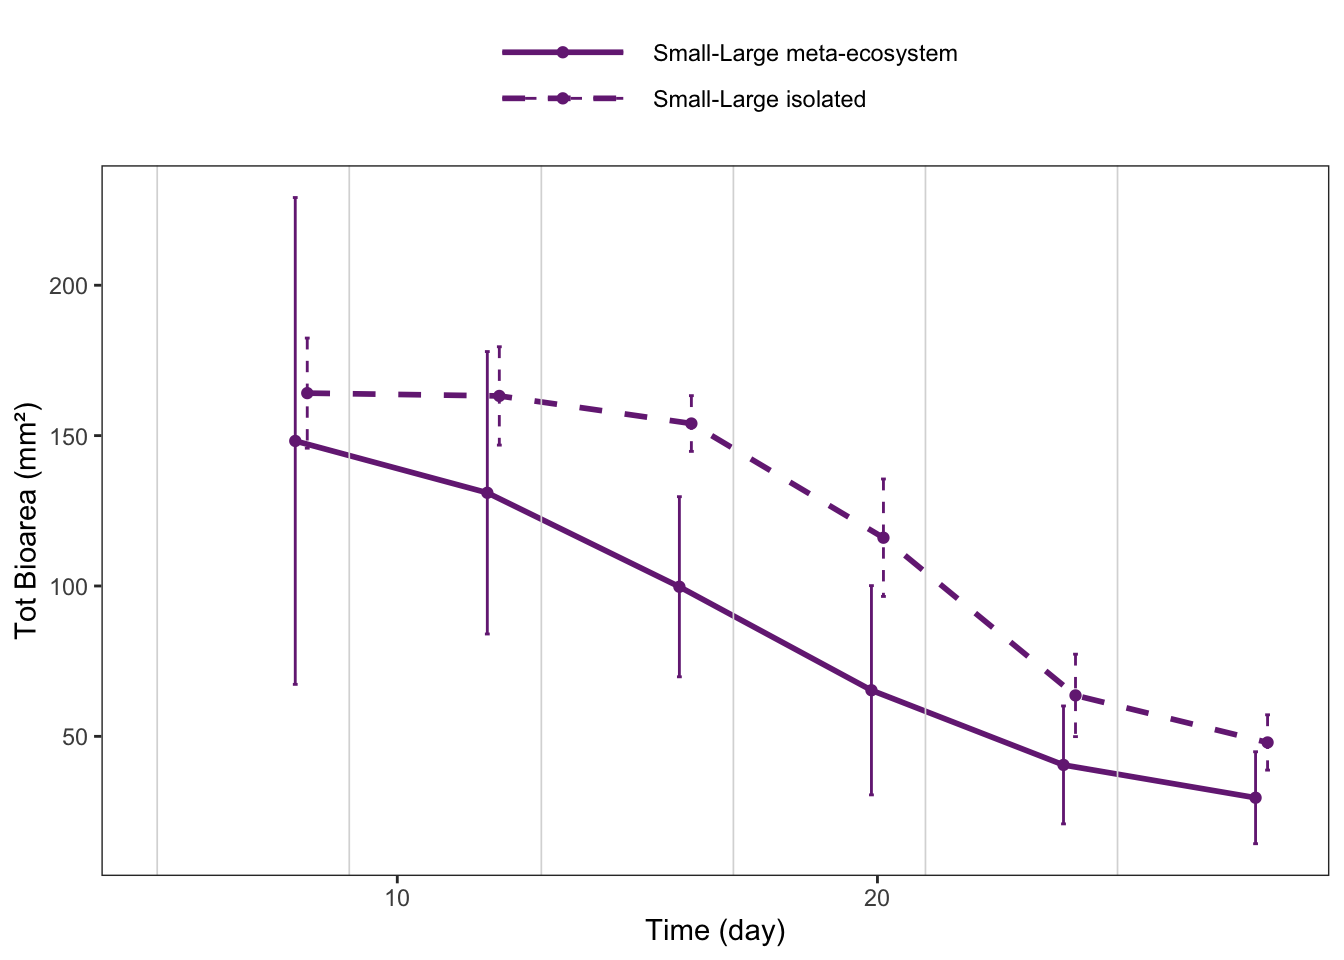
\includegraphics{index_files/figure-latex/unnamed-chunk-187-1.pdf}

\begin{Shaded}
\begin{Highlighting}[]
\FunctionTok{qqnorm}\NormalTok{(}\FunctionTok{resid}\NormalTok{(fixed\_model))}
\end{Highlighting}
\end{Shaded}

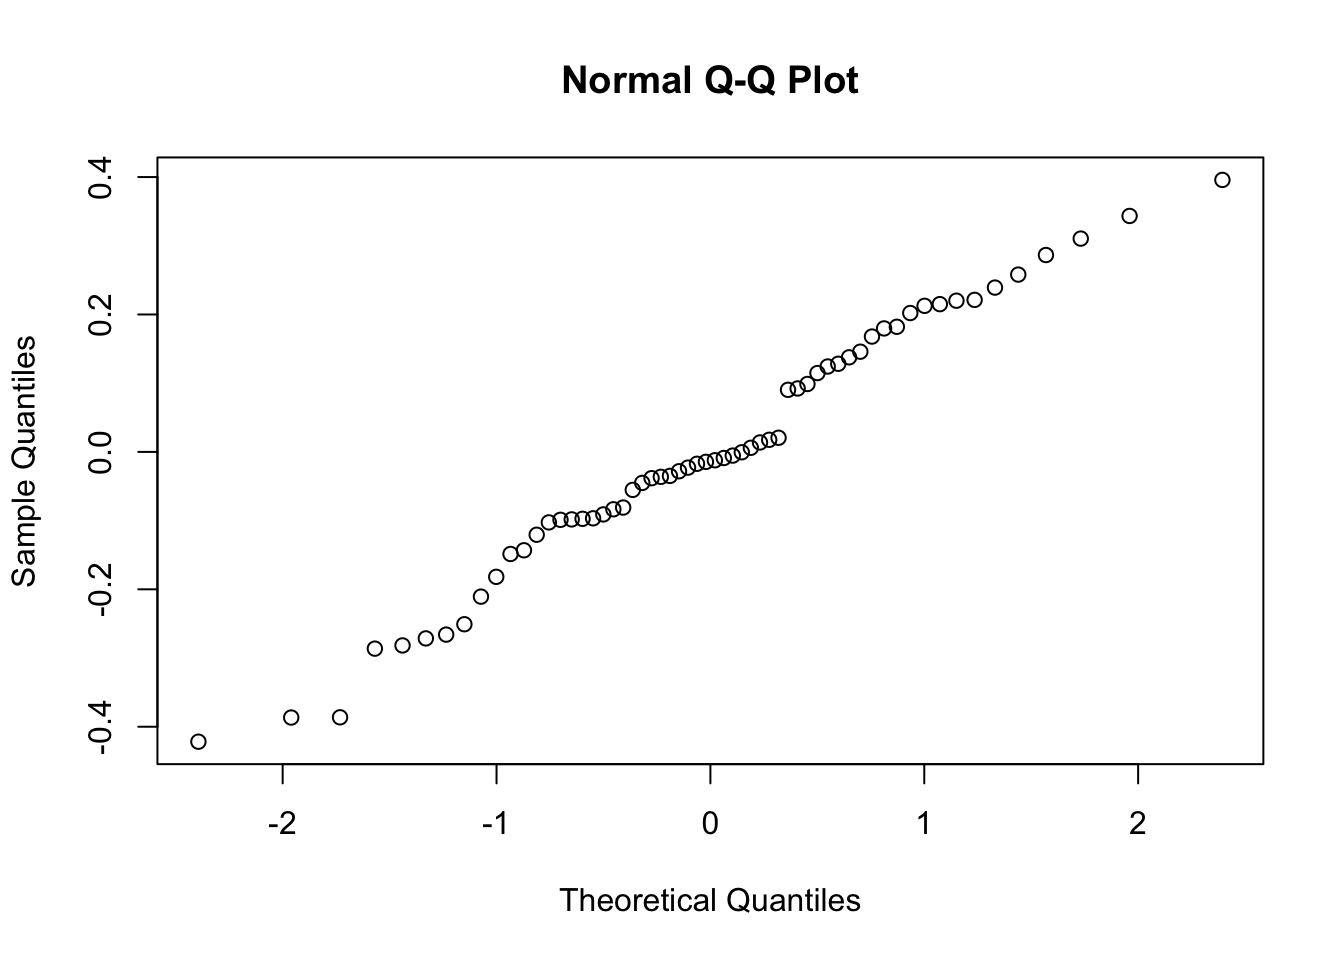
\includegraphics{index_files/figure-latex/unnamed-chunk-187-2.pdf}

\begin{Shaded}
\begin{Highlighting}[]
\NormalTok{model\_stats\_fixed }\OtherTok{=} \FunctionTok{compute.model.stats}\NormalTok{(fixed\_model,}
\NormalTok{                                              null\_model,}
                                              \StringTok{"mixed\_model"}\NormalTok{) }\SpecialCharTok{\%\textgreater{}\%}
  \FunctionTok{print}\NormalTok{()}
\end{Highlighting}
\end{Shaded}

\begin{verbatim}
##    deltaAIC   p_value R2
## 1 0.8942592 0.2930097 NA
\end{verbatim}

\begin{Shaded}
\begin{Highlighting}[]
\NormalTok{results\_table }\OtherTok{=} \FunctionTok{fill.results.table}\NormalTok{(}
\NormalTok{  results\_table,}
\NormalTok{  response\_variable,}
\NormalTok{  metaecosystem\_type\_input\_model,}
\NormalTok{  model\_stats\_full,}
\NormalTok{  model\_stats\_interaction,}
\NormalTok{  model\_stats\_fixed}
\NormalTok{)}
\end{Highlighting}
\end{Shaded}

Small-Large connected vs isolated

\begin{Shaded}
\begin{Highlighting}[]
\NormalTok{metaecosystem\_type\_input\_model }\OtherTok{=} \FunctionTok{c}\NormalTok{(}\StringTok{"Small{-}Large meta{-}ecosystem"}\NormalTok{,}
                                   \StringTok{"Small{-}Large isolated"}\NormalTok{)}
\end{Highlighting}
\end{Shaded}

\begin{Shaded}
\begin{Highlighting}[]
\CommentTok{\#Compute stats for all patch combinations }
\NormalTok{isolated\_combinations\_sets\_filtered }\OtherTok{=}\NormalTok{  isolated\_combinations\_sets }\SpecialCharTok{\%\textgreater{}\%}
  \FunctionTok{filter}\NormalTok{(disturbance }\SpecialCharTok{==}\NormalTok{ disturbance\_global\_input,}
\NormalTok{         metaecosystem\_type }\SpecialCharTok{\%in\%}\NormalTok{ metaecosystem\_type\_input\_model)}

\NormalTok{n\_sets }\OtherTok{=}\NormalTok{ isolated\_combinations\_sets\_filtered }\SpecialCharTok{\%\textgreater{}\%}
  \FunctionTok{pull}\NormalTok{(set) }\SpecialCharTok{\%\textgreater{}\%}
  \FunctionTok{max}\NormalTok{()}

\ControlFlowTok{for}\NormalTok{ (set\_input }\ControlFlowTok{in} \DecValTok{1}\SpecialCharTok{:}\NormalTok{n\_sets) \{}
  
\NormalTok{  system\_nr\_isolated\_systems }\OtherTok{=}\NormalTok{ isolated\_combinations\_sets\_filtered }\SpecialCharTok{\%\textgreater{}\%}
    \FunctionTok{filter}\NormalTok{(}
\NormalTok{      metaecosystem\_type }\SpecialCharTok{\%in\%}\NormalTok{ metaecosystem\_type\_input\_model,}
\NormalTok{      connection }\SpecialCharTok{==} \StringTok{"isolated"}\NormalTok{,}
\NormalTok{      set }\SpecialCharTok{==}\NormalTok{ set\_input}
\NormalTok{    ) }\SpecialCharTok{\%\textgreater{}\%}
    \FunctionTok{pull}\NormalTok{(system\_nr)}
  
\NormalTok{  filtered\_data }\OtherTok{=}\NormalTok{ ds\_metaecosystems }\SpecialCharTok{\%\textgreater{}\%}
    \FunctionTok{filter}\NormalTok{(}
\NormalTok{      time\_point }\SpecialCharTok{\textgreater{}=}\NormalTok{ first\_time\_point\_model,}
\NormalTok{      time\_point }\SpecialCharTok{\textless{}=}\NormalTok{ last\_time\_point\_model,}
\NormalTok{      metaecosystem\_type }\SpecialCharTok{\%in\%}\NormalTok{ metaecosystem\_type\_input\_model,}
\NormalTok{      connection }\SpecialCharTok{==} \StringTok{"connected"} \SpecialCharTok{|}
\NormalTok{        (connection }\SpecialCharTok{==} \StringTok{"isolated"} \SpecialCharTok{\&}
\NormalTok{           system\_nr }\SpecialCharTok{\%in\%}\NormalTok{ system\_nr\_isolated\_systems)}
\NormalTok{    )}
  
\NormalTok{  null\_model }\OtherTok{=} \FunctionTok{lmer}\NormalTok{(}
    \FunctionTok{get}\NormalTok{(response\_variable) }\SpecialCharTok{\textasciitilde{}}
\NormalTok{      day }\SpecialCharTok{+}
\NormalTok{      (day }\SpecialCharTok{|}\NormalTok{ system\_nr),}
    \AttributeTok{data =}\NormalTok{ filtered\_data,}
    \AttributeTok{REML =} \ConstantTok{FALSE}\NormalTok{,}
    \AttributeTok{control =} \FunctionTok{lmerControl}\NormalTok{(}\AttributeTok{optimizer =} \StringTok{"Nelder\_Mead"}\NormalTok{)}
\NormalTok{  )}
  
\NormalTok{  full\_model }\OtherTok{=} \FunctionTok{lmer}\NormalTok{(}
    \FunctionTok{get}\NormalTok{(response\_variable) }\SpecialCharTok{\textasciitilde{}}
\NormalTok{      day }\SpecialCharTok{+}
\NormalTok{      connection }\SpecialCharTok{+}
\NormalTok{      connection}\SpecialCharTok{:}\NormalTok{day }\SpecialCharTok{+}
\NormalTok{      (day }\SpecialCharTok{|}\NormalTok{ system\_nr),}
    \AttributeTok{data =}\NormalTok{ filtered\_data,}
    \AttributeTok{REML =} \ConstantTok{FALSE}\NormalTok{,}
    \AttributeTok{control =} \FunctionTok{lmerControl}\NormalTok{(}\AttributeTok{optimizer =} \StringTok{"Nelder\_Mead"}\NormalTok{)}
\NormalTok{  )}
  
\NormalTok{  model\_stats\_full }\OtherTok{=} \FunctionTok{compute.model.stats}\NormalTok{(full\_model,}
\NormalTok{                                         null\_model,}
                                         \StringTok{"mixed\_model"}\NormalTok{)}
  
\NormalTok{  interaction\_model }\OtherTok{=} \FunctionTok{lmer}\NormalTok{(}
    \FunctionTok{get}\NormalTok{(response\_variable) }\SpecialCharTok{\textasciitilde{}}
\NormalTok{      day }\SpecialCharTok{+}
\NormalTok{      connection}\SpecialCharTok{:}\NormalTok{day }\SpecialCharTok{+}
\NormalTok{      (day }\SpecialCharTok{|}\NormalTok{ system\_nr),}
    \AttributeTok{data =}\NormalTok{ filtered\_data,}
    \AttributeTok{REML =} \ConstantTok{FALSE}\NormalTok{,}
    \AttributeTok{control =} \FunctionTok{lmerControl}\NormalTok{(}\AttributeTok{optimizer =} \StringTok{"Nelder\_Mead"}\NormalTok{)}
\NormalTok{  )}
  
\NormalTok{  model\_stats\_interaction }\OtherTok{=} \FunctionTok{compute.model.stats}\NormalTok{(interaction\_model,}
\NormalTok{                                                null\_model,}
                                                \StringTok{"mixed\_model"}\NormalTok{)}
  
\NormalTok{  fixed\_model }\OtherTok{=} \FunctionTok{lmer}\NormalTok{(}
    \FunctionTok{get}\NormalTok{(response\_variable) }\SpecialCharTok{\textasciitilde{}}
\NormalTok{      day }\SpecialCharTok{+}
\NormalTok{      connection }\SpecialCharTok{+}
\NormalTok{      (day }\SpecialCharTok{|}\NormalTok{ system\_nr),}
    \AttributeTok{data =}\NormalTok{ filtered\_data,}
    \AttributeTok{REML =} \ConstantTok{FALSE}\NormalTok{,}
    \AttributeTok{control =} \FunctionTok{lmerControl}\NormalTok{(}\AttributeTok{optimizer =} \StringTok{"Nelder\_Mead"}\NormalTok{)}
\NormalTok{  )}
  
\NormalTok{  model\_stats\_fixed }\OtherTok{=} \FunctionTok{compute.model.stats}\NormalTok{(fixed\_model,}
\NormalTok{                                          null\_model,}
                                          \StringTok{"mixed\_model"}\NormalTok{)}
  
\NormalTok{  iterated\_results\_table }\OtherTok{=} \FunctionTok{fill.results.table}\NormalTok{(}
\NormalTok{    iterated\_results\_table,}
\NormalTok{    response\_variable,}
\NormalTok{    metaecosystem\_type\_input\_model,}
\NormalTok{    model\_stats\_full,}
\NormalTok{    model\_stats\_interaction,}
\NormalTok{    model\_stats\_fixed}
\NormalTok{  )}
  
\NormalTok{  iterated\_results\_table}\SpecialCharTok{$}\NormalTok{set }\OtherTok{=}\NormalTok{ set\_input}
\NormalTok{\}}
\end{Highlighting}
\end{Shaded}

\begin{Shaded}
\begin{Highlighting}[]
\CommentTok{\#Check that there\textquotesingle{}s nothing wired with the AIC and p{-}value distributions }
\FunctionTok{hist}\NormalTok{(iterated\_results\_table}\SpecialCharTok{$}\NormalTok{ΔAIC\_full, }\AttributeTok{main =} \StringTok{"Distribution of ΔAIC of the full model."}\NormalTok{) }
\end{Highlighting}
\end{Shaded}

\begin{verbatim}
## Warning in title(main = main, sub = sub, xlab = xlab, ylab = ylab, ...):
## conversion failure on 'Distribution of ΔAIC of the full model.' in 'mbcsToSbcs':
## dot substituted for <ce>
\end{verbatim}

\begin{verbatim}
## Warning in title(main = main, sub = sub, xlab = xlab, ylab = ylab, ...):
## conversion failure on 'Distribution of ΔAIC of the full model.' in 'mbcsToSbcs':
## dot substituted for <94>
\end{verbatim}

\begin{verbatim}
## Warning in title(main = main, sub = sub, xlab = xlab, ylab = ylab, ...):
## conversion failure on 'iterated_results_table$ΔAIC_full' in 'mbcsToSbcs': dot
## substituted for <ce>
\end{verbatim}

\begin{verbatim}
## Warning in title(main = main, sub = sub, xlab = xlab, ylab = ylab, ...):
## conversion failure on 'iterated_results_table$ΔAIC_full' in 'mbcsToSbcs': dot
## substituted for <94>
\end{verbatim}

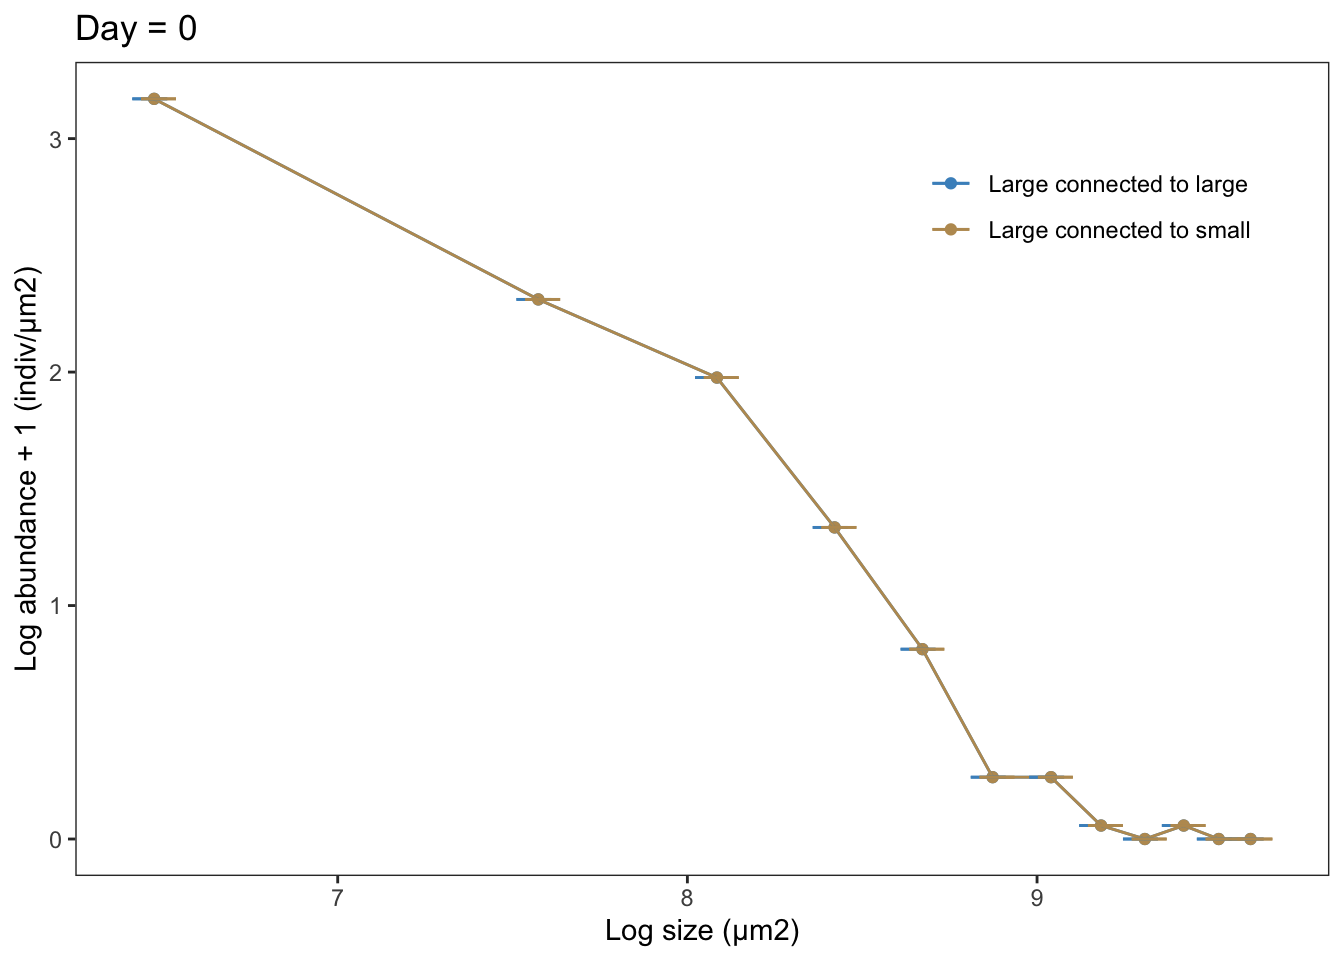
\includegraphics{index_files/figure-latex/unnamed-chunk-190-1.pdf}

\begin{Shaded}
\begin{Highlighting}[]
\FunctionTok{hist}\NormalTok{(iterated\_results\_table}\SpecialCharTok{$}\NormalTok{p\_full, }\AttributeTok{main =} \StringTok{"Distribution of p{-}values of the full model."}\NormalTok{) }
\end{Highlighting}
\end{Shaded}

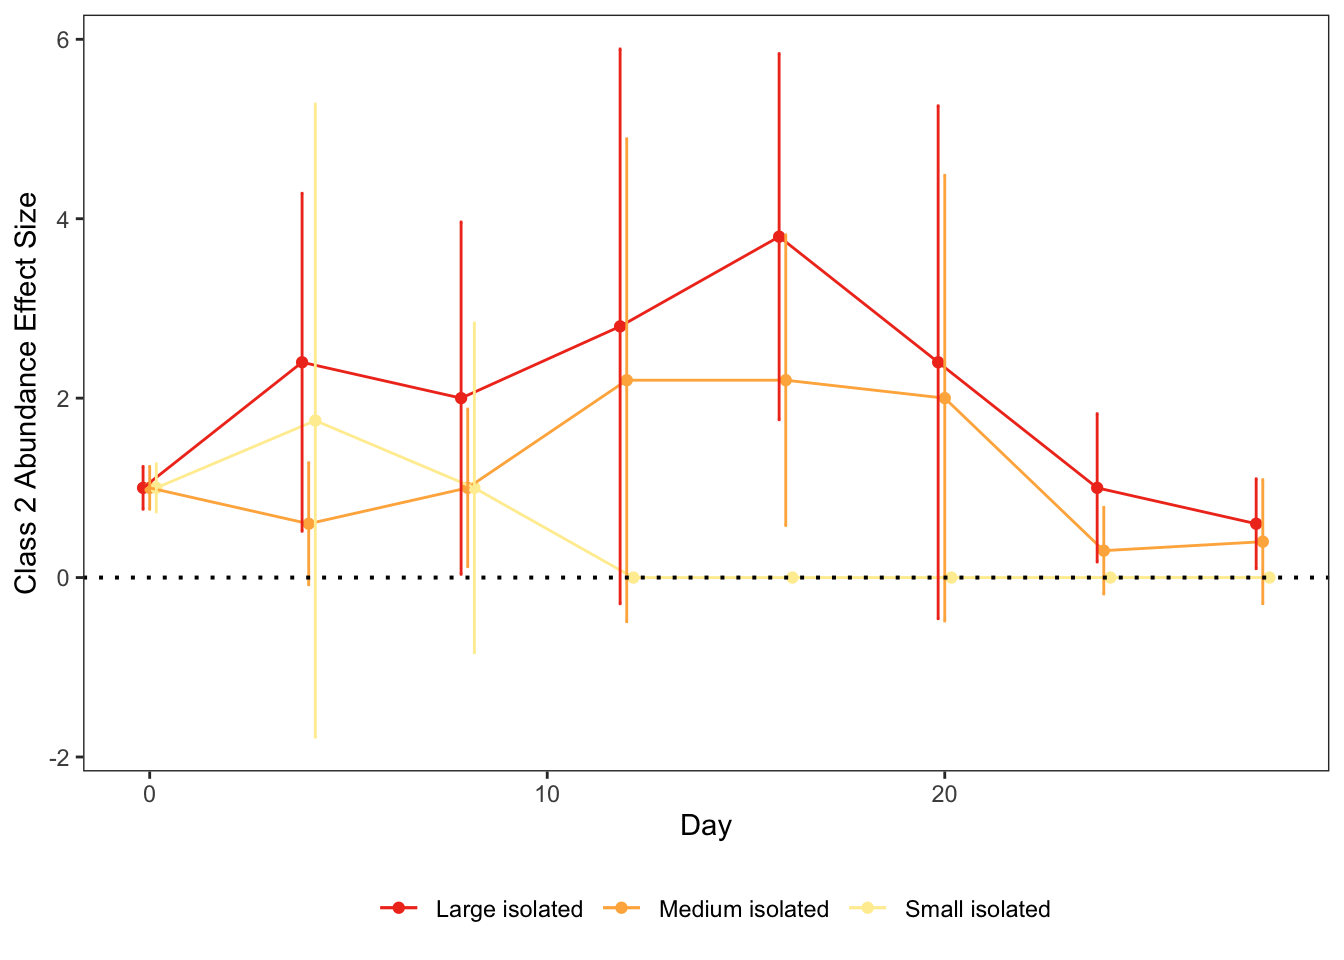
\includegraphics{index_files/figure-latex/unnamed-chunk-190-2.pdf}

\begin{Shaded}
\begin{Highlighting}[]
\FunctionTok{hist}\NormalTok{(iterated\_results\_table}\SpecialCharTok{$}\NormalTok{ΔAIC\_fix, }\AttributeTok{main =} \StringTok{"Distribution of ΔAIC of the fixed model."}\NormalTok{) }
\end{Highlighting}
\end{Shaded}

\begin{verbatim}
## Warning in title(main = main, sub = sub, xlab = xlab, ylab = ylab, ...):
## conversion failure on 'Distribution of ΔAIC of the fixed model.' in
## 'mbcsToSbcs': dot substituted for <ce>
\end{verbatim}

\begin{verbatim}
## Warning in title(main = main, sub = sub, xlab = xlab, ylab = ylab, ...):
## conversion failure on 'Distribution of ΔAIC of the fixed model.' in
## 'mbcsToSbcs': dot substituted for <94>
\end{verbatim}

\begin{verbatim}
## Warning in title(main = main, sub = sub, xlab = xlab, ylab = ylab, ...):
## conversion failure on 'iterated_results_table$ΔAIC_fix' in 'mbcsToSbcs': dot
## substituted for <ce>
\end{verbatim}

\begin{verbatim}
## Warning in title(main = main, sub = sub, xlab = xlab, ylab = ylab, ...):
## conversion failure on 'iterated_results_table$ΔAIC_fix' in 'mbcsToSbcs': dot
## substituted for <94>
\end{verbatim}

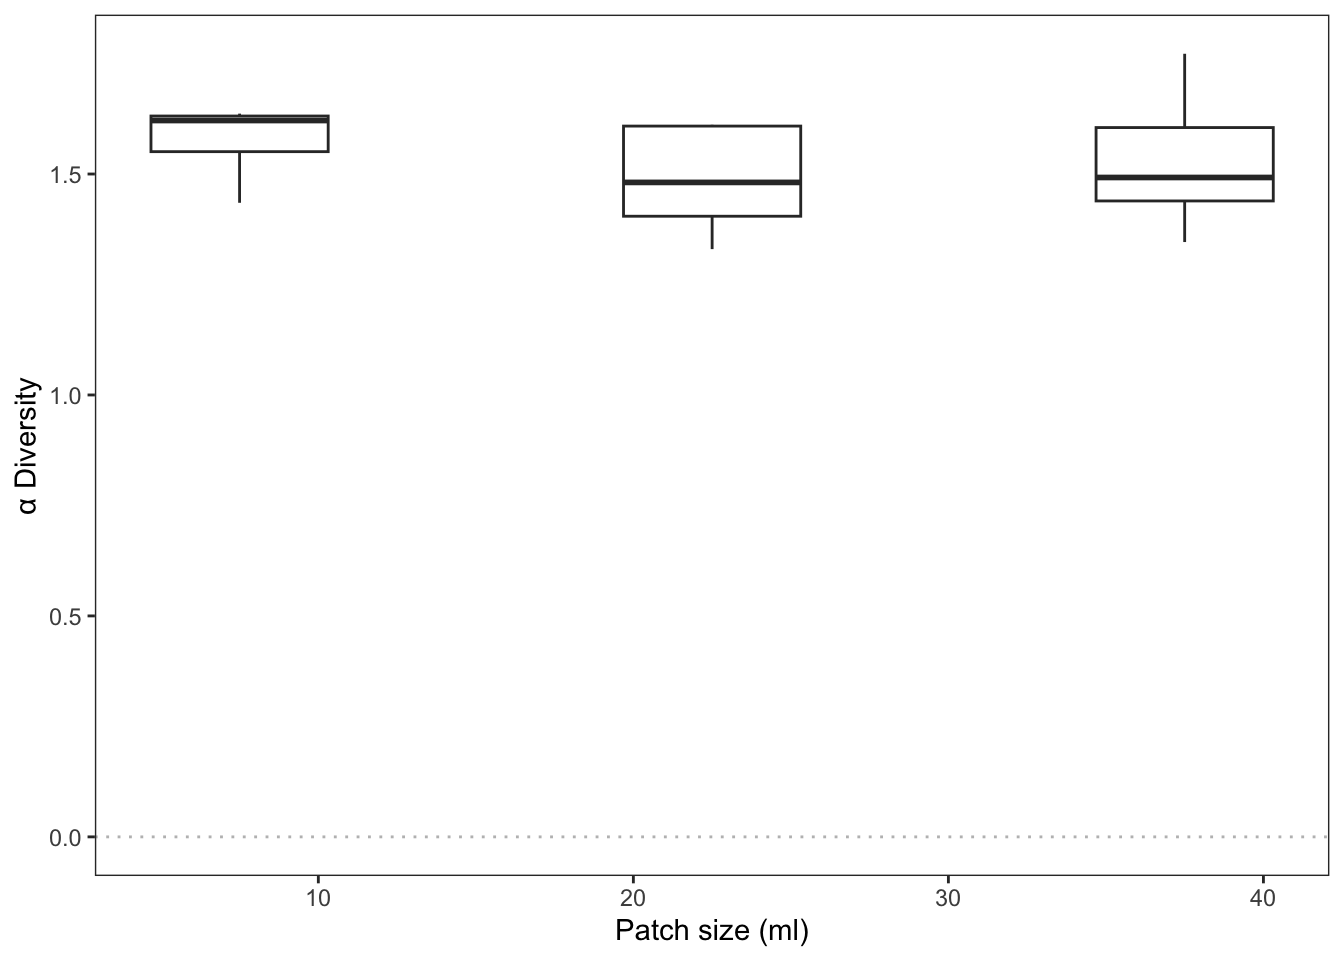
\includegraphics{index_files/figure-latex/unnamed-chunk-190-3.pdf}

\begin{Shaded}
\begin{Highlighting}[]
\FunctionTok{hist}\NormalTok{(iterated\_results\_table}\SpecialCharTok{$}\NormalTok{p\_fix, }\AttributeTok{main =} \StringTok{"Distribution of p{-}values of the fixed model."}\NormalTok{) }
\end{Highlighting}
\end{Shaded}

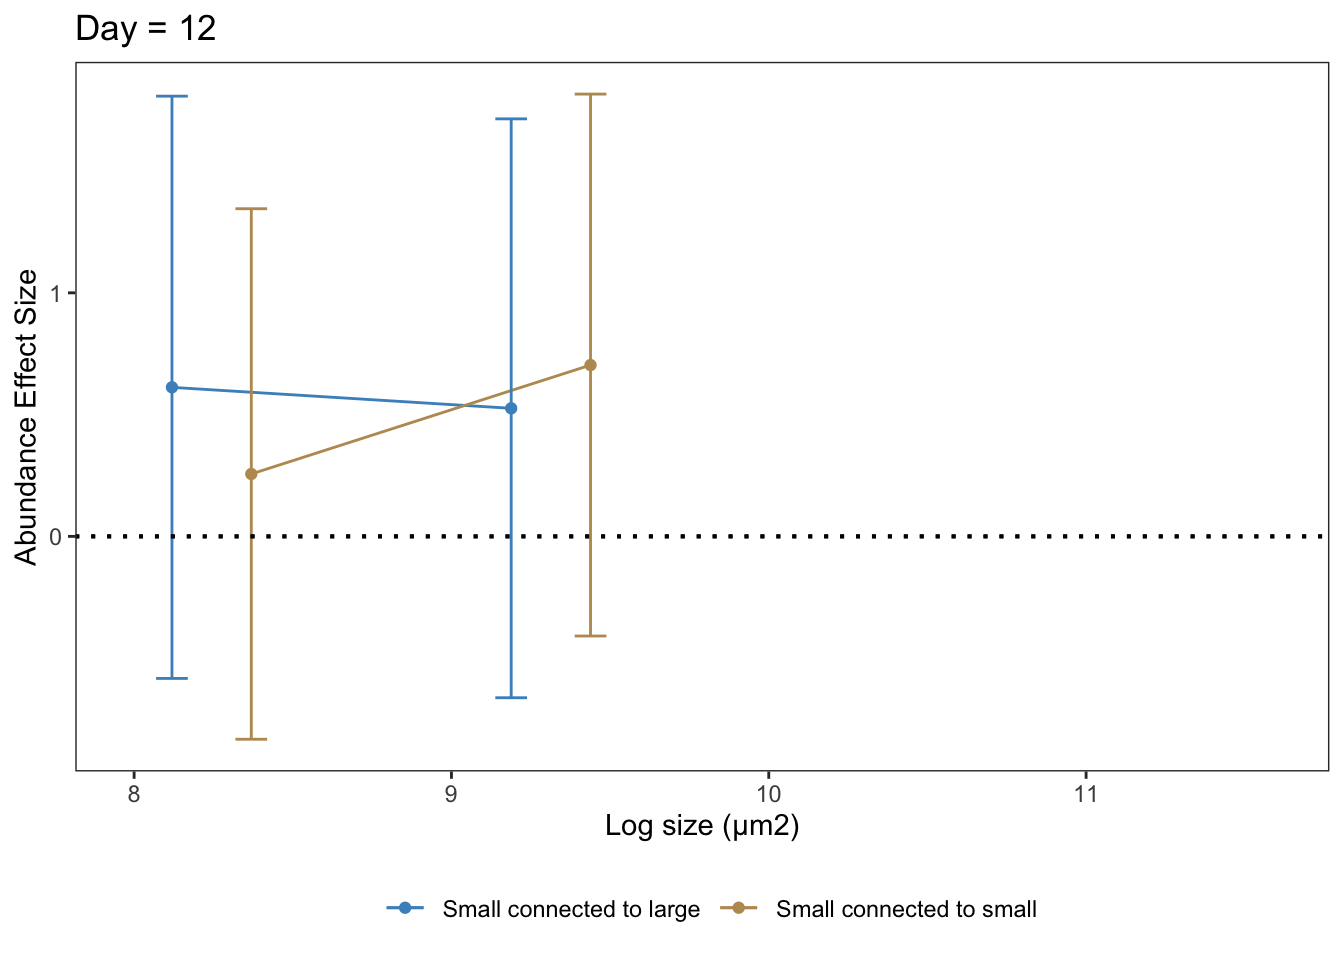
\includegraphics{index_files/figure-latex/unnamed-chunk-190-4.pdf}

\begin{Shaded}
\begin{Highlighting}[]
\FunctionTok{hist}\NormalTok{(iterated\_results\_table}\SpecialCharTok{$}\NormalTok{ΔAIC\_int, }\AttributeTok{main =} \StringTok{"Distribution of ΔAIC of the interation model."}\NormalTok{) }
\end{Highlighting}
\end{Shaded}

\begin{verbatim}
## Warning in title(main = main, sub = sub, xlab = xlab, ylab = ylab, ...):
## conversion failure on 'Distribution of ΔAIC of the interation model.' in
## 'mbcsToSbcs': dot substituted for <ce>
\end{verbatim}

\begin{verbatim}
## Warning in title(main = main, sub = sub, xlab = xlab, ylab = ylab, ...):
## conversion failure on 'Distribution of ΔAIC of the interation model.' in
## 'mbcsToSbcs': dot substituted for <94>
\end{verbatim}

\begin{verbatim}
## Warning in title(main = main, sub = sub, xlab = xlab, ylab = ylab, ...):
## conversion failure on 'iterated_results_table$ΔAIC_int' in 'mbcsToSbcs': dot
## substituted for <ce>
\end{verbatim}

\begin{verbatim}
## Warning in title(main = main, sub = sub, xlab = xlab, ylab = ylab, ...):
## conversion failure on 'iterated_results_table$ΔAIC_int' in 'mbcsToSbcs': dot
## substituted for <94>
\end{verbatim}

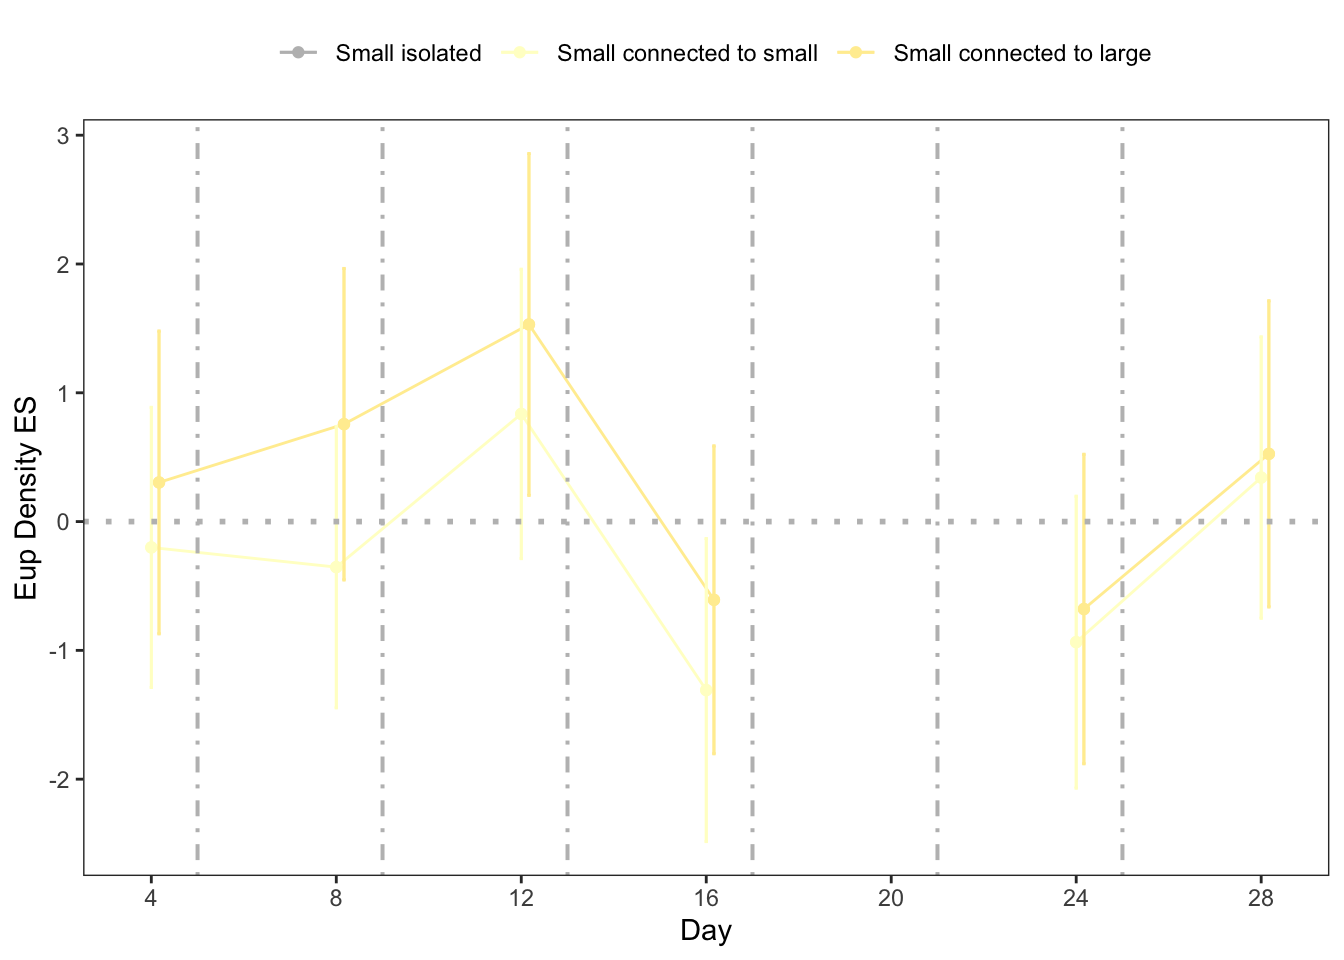
\includegraphics{index_files/figure-latex/unnamed-chunk-190-5.pdf}

\begin{Shaded}
\begin{Highlighting}[]
\FunctionTok{hist}\NormalTok{(iterated\_results\_table}\SpecialCharTok{$}\NormalTok{p\_int, }\AttributeTok{main =} \StringTok{"Distribution of p{-}values of the interation model."}\NormalTok{) }
\end{Highlighting}
\end{Shaded}

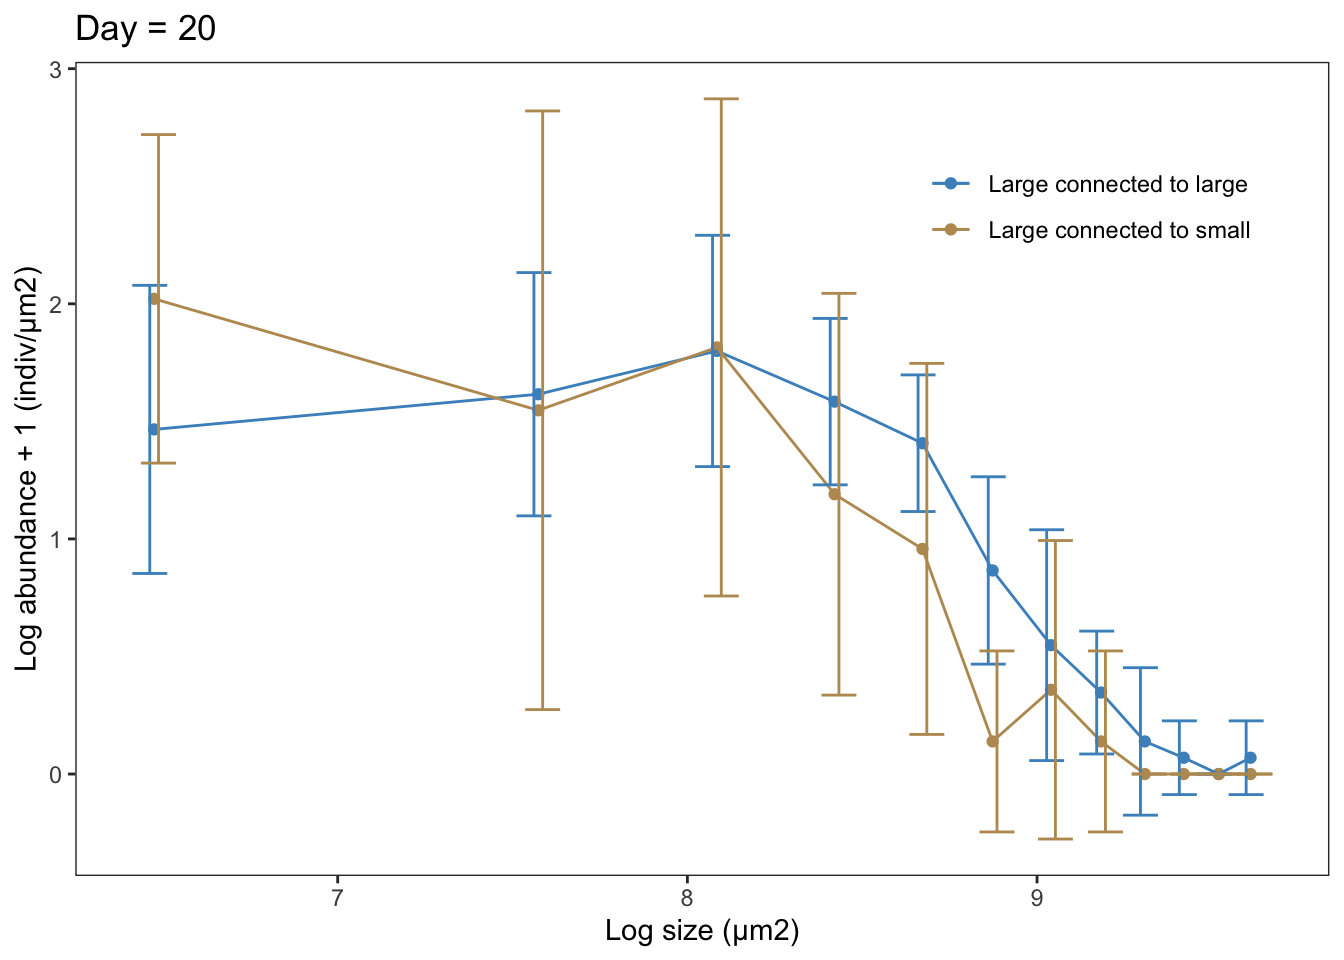
\includegraphics{index_files/figure-latex/unnamed-chunk-190-6.pdf}

\begin{Shaded}
\begin{Highlighting}[]
\CommentTok{\#Use the mean p{-}values and ΔAIC }
\NormalTok{model\_stats\_full }\OtherTok{=} \FunctionTok{data.frame}\NormalTok{(}
  \AttributeTok{deltaAIC =} \FunctionTok{mean}\NormalTok{(iterated\_results\_table}\SpecialCharTok{$}\NormalTok{ΔAIC\_full),}
  \AttributeTok{p\_value =} \FunctionTok{mean}\NormalTok{(iterated\_results\_table}\SpecialCharTok{$}\NormalTok{p\_full),}
  \AttributeTok{R2 =} \ConstantTok{NA}
\NormalTok{) }

\NormalTok{model\_stats\_interaction }\OtherTok{=} \FunctionTok{data.frame}\NormalTok{(}
  \AttributeTok{deltaAIC =} \FunctionTok{mean}\NormalTok{(iterated\_results\_table}\SpecialCharTok{$}\NormalTok{ΔAIC\_int),}
  \AttributeTok{p\_value =} \FunctionTok{mean}\NormalTok{(iterated\_results\_table}\SpecialCharTok{$}\NormalTok{p\_int),}
  \AttributeTok{R2 =} \ConstantTok{NA}
\NormalTok{)}

\NormalTok{model\_stats\_fixed }\OtherTok{=} \FunctionTok{data.frame}\NormalTok{(}
  \AttributeTok{deltaAIC =} \FunctionTok{mean}\NormalTok{(iterated\_results\_table}\SpecialCharTok{$}\NormalTok{ΔAIC\_fix),}
  \AttributeTok{p\_value =} \FunctionTok{mean}\NormalTok{(iterated\_results\_table}\SpecialCharTok{$}\NormalTok{p\_fix),}
  \AttributeTok{R2 =} \ConstantTok{NA}
\NormalTok{)}

\NormalTok{results\_table }\OtherTok{=} \FunctionTok{fill.results.table}\NormalTok{(}
\NormalTok{    results\_table,}
\NormalTok{    response\_variable,}
\NormalTok{    metaecosystem\_type\_input\_model,}
\NormalTok{    model\_stats\_full,}
\NormalTok{    model\_stats\_interaction,}
\NormalTok{    model\_stats\_fixed}
\NormalTok{  )}
\end{Highlighting}
\end{Shaded}

Medium-Medium connected vs isolated

\begin{Shaded}
\begin{Highlighting}[]
\NormalTok{metaecosystem\_type\_input\_model }\OtherTok{=} \FunctionTok{c}\NormalTok{(}\StringTok{"Medium{-}Medium meta{-}ecosystem"}\NormalTok{,}
                                   \StringTok{"Medium{-}Medium isolated"}\NormalTok{)}
\end{Highlighting}
\end{Shaded}

\begin{Shaded}
\begin{Highlighting}[]
\CommentTok{\#Compute stats for all patch combinations }
\NormalTok{isolated\_combinations\_sets\_filtered }\OtherTok{=}\NormalTok{  isolated\_combinations\_sets }\SpecialCharTok{\%\textgreater{}\%}
  \FunctionTok{filter}\NormalTok{(disturbance }\SpecialCharTok{==}\NormalTok{ disturbance\_global\_input,}
\NormalTok{         metaecosystem\_type }\SpecialCharTok{\%in\%}\NormalTok{ metaecosystem\_type\_input\_model)}

\NormalTok{n\_sets }\OtherTok{=}\NormalTok{ isolated\_combinations\_sets\_filtered }\SpecialCharTok{\%\textgreater{}\%}
  \FunctionTok{pull}\NormalTok{(set) }\SpecialCharTok{\%\textgreater{}\%}
  \FunctionTok{max}\NormalTok{()}

\ControlFlowTok{for}\NormalTok{ (set\_input }\ControlFlowTok{in} \DecValTok{1}\SpecialCharTok{:}\NormalTok{n\_sets) \{}
  
\NormalTok{  system\_nr\_isolated\_systems }\OtherTok{=}\NormalTok{ isolated\_combinations\_sets\_filtered }\SpecialCharTok{\%\textgreater{}\%}
    \FunctionTok{filter}\NormalTok{(}
\NormalTok{      metaecosystem\_type }\SpecialCharTok{\%in\%}\NormalTok{ metaecosystem\_type\_input\_model,}
\NormalTok{      connection }\SpecialCharTok{==} \StringTok{"isolated"}\NormalTok{,}
\NormalTok{      set }\SpecialCharTok{==}\NormalTok{ set\_input}
\NormalTok{    ) }\SpecialCharTok{\%\textgreater{}\%}
    \FunctionTok{pull}\NormalTok{(system\_nr)}
  
\NormalTok{  filtered\_data }\OtherTok{=}\NormalTok{ ds\_metaecosystems }\SpecialCharTok{\%\textgreater{}\%}
    \FunctionTok{filter}\NormalTok{(}
\NormalTok{      time\_point }\SpecialCharTok{\textgreater{}=}\NormalTok{ first\_time\_point\_model,}
\NormalTok{      time\_point }\SpecialCharTok{\textless{}=}\NormalTok{ last\_time\_point\_model,}
\NormalTok{      metaecosystem\_type }\SpecialCharTok{\%in\%}\NormalTok{ metaecosystem\_type\_input\_model,}
\NormalTok{      connection }\SpecialCharTok{==} \StringTok{"connected"} \SpecialCharTok{|}
\NormalTok{        (connection }\SpecialCharTok{==} \StringTok{"isolated"} \SpecialCharTok{\&}
\NormalTok{           system\_nr }\SpecialCharTok{\%in\%}\NormalTok{ system\_nr\_isolated\_systems)}
\NormalTok{    )}
  
\NormalTok{  null\_model }\OtherTok{=} \FunctionTok{lmer}\NormalTok{(}
    \FunctionTok{get}\NormalTok{(response\_variable) }\SpecialCharTok{\textasciitilde{}}
\NormalTok{      day }\SpecialCharTok{+}
\NormalTok{      (day }\SpecialCharTok{|}\NormalTok{ system\_nr),}
    \AttributeTok{data =}\NormalTok{ filtered\_data,}
    \AttributeTok{REML =} \ConstantTok{FALSE}\NormalTok{,}
    \AttributeTok{control =} \FunctionTok{lmerControl}\NormalTok{(}\AttributeTok{optimizer =} \StringTok{"Nelder\_Mead"}\NormalTok{)}
\NormalTok{  )}
  
\NormalTok{  full\_model }\OtherTok{=} \FunctionTok{lmer}\NormalTok{(}
    \FunctionTok{get}\NormalTok{(response\_variable) }\SpecialCharTok{\textasciitilde{}}
\NormalTok{      day }\SpecialCharTok{+}
\NormalTok{      connection }\SpecialCharTok{+}
\NormalTok{      connection}\SpecialCharTok{:}\NormalTok{day }\SpecialCharTok{+}
\NormalTok{      (day }\SpecialCharTok{|}\NormalTok{ system\_nr),}
    \AttributeTok{data =}\NormalTok{ filtered\_data,}
    \AttributeTok{REML =} \ConstantTok{FALSE}\NormalTok{,}
    \AttributeTok{control =} \FunctionTok{lmerControl}\NormalTok{(}\AttributeTok{optimizer =} \StringTok{"Nelder\_Mead"}\NormalTok{)}
\NormalTok{  )}
  
\NormalTok{  model\_stats\_full }\OtherTok{=} \FunctionTok{compute.model.stats}\NormalTok{(full\_model,}
\NormalTok{                                         null\_model,}
                                         \StringTok{"mixed\_model"}\NormalTok{)}
  
\NormalTok{  interaction\_model }\OtherTok{=} \FunctionTok{lmer}\NormalTok{(}
    \FunctionTok{get}\NormalTok{(response\_variable) }\SpecialCharTok{\textasciitilde{}}
\NormalTok{      day }\SpecialCharTok{+}
\NormalTok{      connection}\SpecialCharTok{:}\NormalTok{day }\SpecialCharTok{+}
\NormalTok{      (day }\SpecialCharTok{|}\NormalTok{ system\_nr),}
    \AttributeTok{data =}\NormalTok{ filtered\_data,}
    \AttributeTok{REML =} \ConstantTok{FALSE}\NormalTok{,}
    \AttributeTok{control =} \FunctionTok{lmerControl}\NormalTok{(}\AttributeTok{optimizer =} \StringTok{"Nelder\_Mead"}\NormalTok{)}
\NormalTok{  )}
  
\NormalTok{  model\_stats\_interaction }\OtherTok{=} \FunctionTok{compute.model.stats}\NormalTok{(interaction\_model,}
\NormalTok{                                                null\_model,}
                                                \StringTok{"mixed\_model"}\NormalTok{)}
  
\NormalTok{  fixed\_model }\OtherTok{=} \FunctionTok{lmer}\NormalTok{(}
    \FunctionTok{get}\NormalTok{(response\_variable) }\SpecialCharTok{\textasciitilde{}}
\NormalTok{      day }\SpecialCharTok{+}
\NormalTok{      connection }\SpecialCharTok{+}
\NormalTok{      (day }\SpecialCharTok{|}\NormalTok{ system\_nr),}
    \AttributeTok{data =}\NormalTok{ filtered\_data,}
    \AttributeTok{REML =} \ConstantTok{FALSE}\NormalTok{,}
    \AttributeTok{control =} \FunctionTok{lmerControl}\NormalTok{(}\AttributeTok{optimizer =} \StringTok{"Nelder\_Mead"}\NormalTok{)}
\NormalTok{  )}
  
\NormalTok{  model\_stats\_fixed }\OtherTok{=} \FunctionTok{compute.model.stats}\NormalTok{(fixed\_model,}
\NormalTok{                                          null\_model,}
                                          \StringTok{"mixed\_model"}\NormalTok{)}
  
\NormalTok{  iterated\_results\_table }\OtherTok{=} \FunctionTok{fill.results.table}\NormalTok{(}
\NormalTok{    iterated\_results\_table,}
\NormalTok{    response\_variable,}
\NormalTok{    metaecosystem\_type\_input\_model,}
\NormalTok{    model\_stats\_full,}
\NormalTok{    model\_stats\_interaction,}
\NormalTok{    model\_stats\_fixed}
\NormalTok{  )}
  
\NormalTok{  iterated\_results\_table}\SpecialCharTok{$}\NormalTok{set }\OtherTok{=}\NormalTok{ set\_input}
\NormalTok{\}}
\end{Highlighting}
\end{Shaded}

\begin{Shaded}
\begin{Highlighting}[]
\CommentTok{\#Check that there\textquotesingle{}s nothing wired with the AIC and p{-}value distributions }
\FunctionTok{hist}\NormalTok{(iterated\_results\_table}\SpecialCharTok{$}\NormalTok{ΔAIC\_full, }\AttributeTok{main =} \StringTok{"Distribution of ΔAIC of the full model."}\NormalTok{) }
\end{Highlighting}
\end{Shaded}

\begin{verbatim}
## Warning in title(main = main, sub = sub, xlab = xlab, ylab = ylab, ...):
## conversion failure on 'Distribution of ΔAIC of the full model.' in 'mbcsToSbcs':
## dot substituted for <ce>
\end{verbatim}

\begin{verbatim}
## Warning in title(main = main, sub = sub, xlab = xlab, ylab = ylab, ...):
## conversion failure on 'Distribution of ΔAIC of the full model.' in 'mbcsToSbcs':
## dot substituted for <94>
\end{verbatim}

\begin{verbatim}
## Warning in title(main = main, sub = sub, xlab = xlab, ylab = ylab, ...):
## conversion failure on 'iterated_results_table$ΔAIC_full' in 'mbcsToSbcs': dot
## substituted for <ce>
\end{verbatim}

\begin{verbatim}
## Warning in title(main = main, sub = sub, xlab = xlab, ylab = ylab, ...):
## conversion failure on 'iterated_results_table$ΔAIC_full' in 'mbcsToSbcs': dot
## substituted for <94>
\end{verbatim}

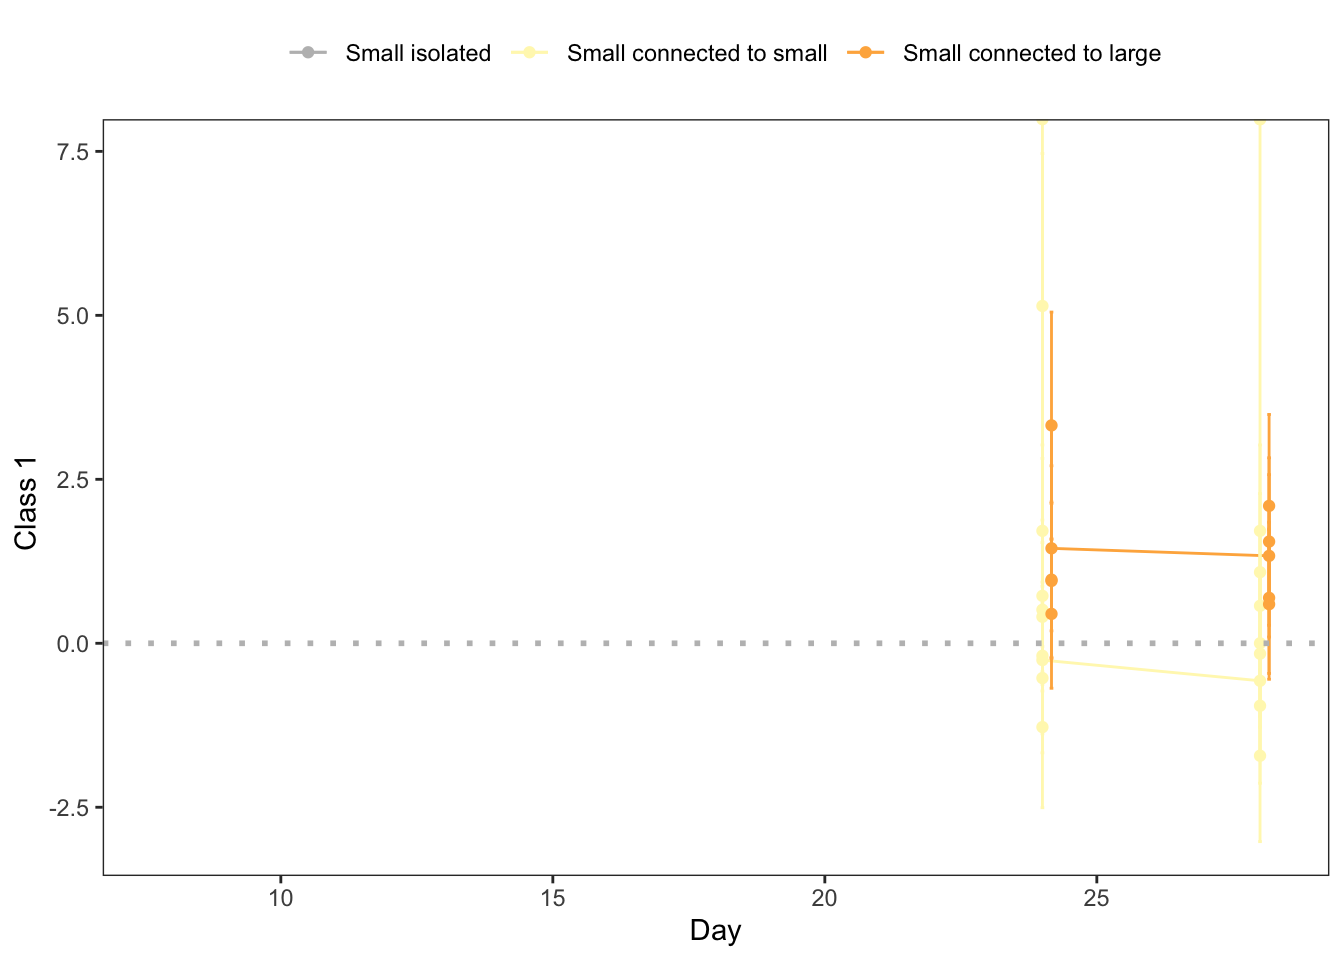
\includegraphics{index_files/figure-latex/unnamed-chunk-193-1.pdf}

\begin{Shaded}
\begin{Highlighting}[]
\FunctionTok{hist}\NormalTok{(iterated\_results\_table}\SpecialCharTok{$}\NormalTok{p\_full, }\AttributeTok{main =} \StringTok{"Distribution of p{-}values of the full model."}\NormalTok{) }
\end{Highlighting}
\end{Shaded}

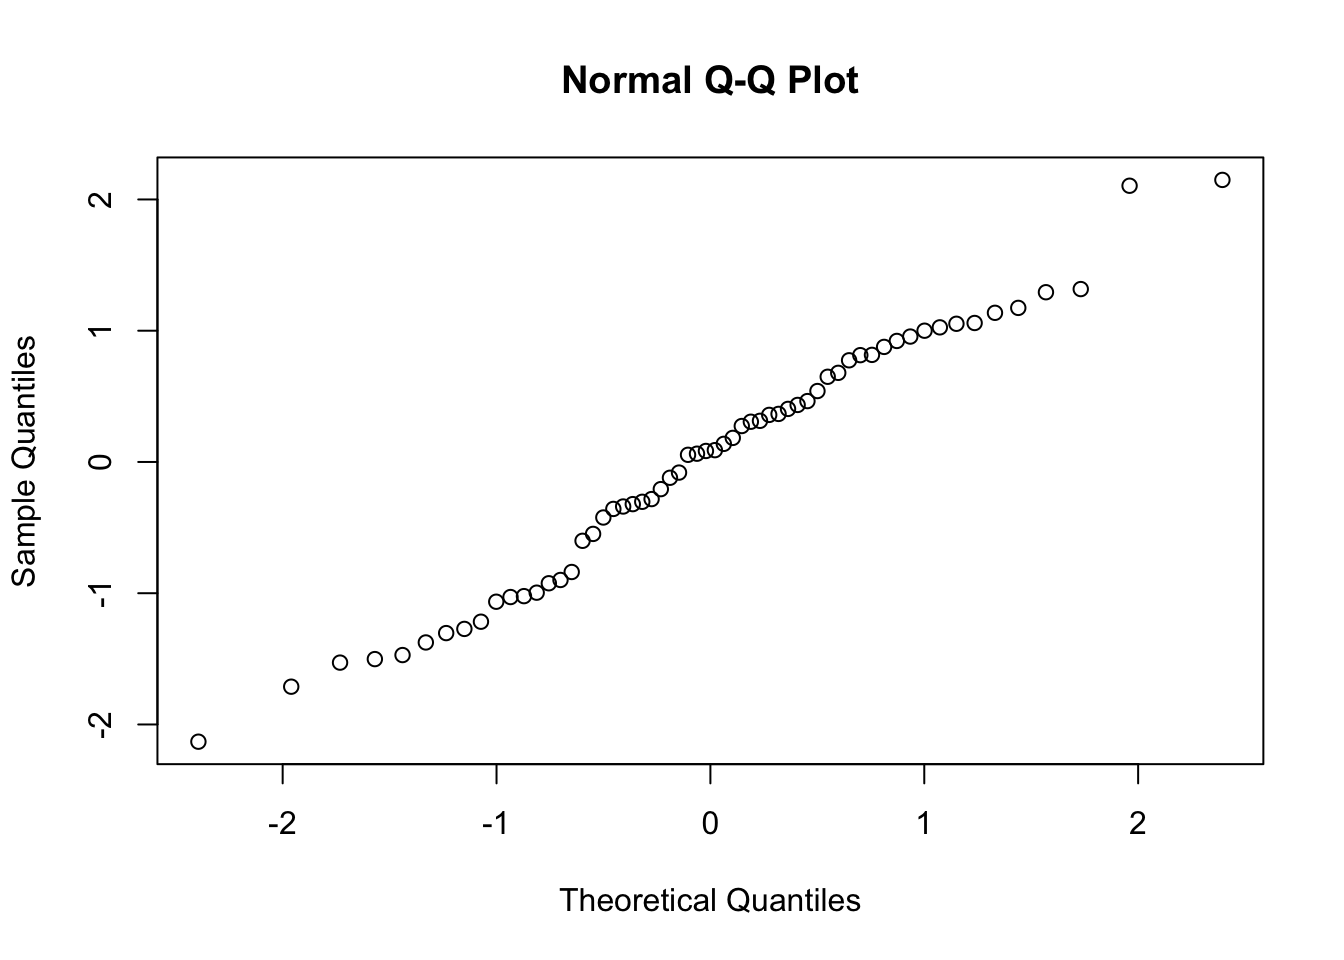
\includegraphics{index_files/figure-latex/unnamed-chunk-193-2.pdf}

\begin{Shaded}
\begin{Highlighting}[]
\FunctionTok{hist}\NormalTok{(iterated\_results\_table}\SpecialCharTok{$}\NormalTok{ΔAIC\_fix, }\AttributeTok{main =} \StringTok{"Distribution of ΔAIC of the fixed model."}\NormalTok{) }
\end{Highlighting}
\end{Shaded}

\begin{verbatim}
## Warning in title(main = main, sub = sub, xlab = xlab, ylab = ylab, ...):
## conversion failure on 'Distribution of ΔAIC of the fixed model.' in
## 'mbcsToSbcs': dot substituted for <ce>
\end{verbatim}

\begin{verbatim}
## Warning in title(main = main, sub = sub, xlab = xlab, ylab = ylab, ...):
## conversion failure on 'Distribution of ΔAIC of the fixed model.' in
## 'mbcsToSbcs': dot substituted for <94>
\end{verbatim}

\begin{verbatim}
## Warning in title(main = main, sub = sub, xlab = xlab, ylab = ylab, ...):
## conversion failure on 'iterated_results_table$ΔAIC_fix' in 'mbcsToSbcs': dot
## substituted for <ce>
\end{verbatim}

\begin{verbatim}
## Warning in title(main = main, sub = sub, xlab = xlab, ylab = ylab, ...):
## conversion failure on 'iterated_results_table$ΔAIC_fix' in 'mbcsToSbcs': dot
## substituted for <94>
\end{verbatim}

\includegraphics{index_files/figure-latex/unnamed-chunk-193-3.pdf}

\begin{Shaded}
\begin{Highlighting}[]
\FunctionTok{hist}\NormalTok{(iterated\_results\_table}\SpecialCharTok{$}\NormalTok{p\_fix, }\AttributeTok{main =} \StringTok{"Distribution of p{-}values of the fixed model."}\NormalTok{) }
\end{Highlighting}
\end{Shaded}

\includegraphics{index_files/figure-latex/unnamed-chunk-193-4.pdf}

\begin{Shaded}
\begin{Highlighting}[]
\FunctionTok{hist}\NormalTok{(iterated\_results\_table}\SpecialCharTok{$}\NormalTok{ΔAIC\_int, }\AttributeTok{main =} \StringTok{"Distribution of ΔAIC of the interation model."}\NormalTok{) }
\end{Highlighting}
\end{Shaded}

\begin{verbatim}
## Warning in title(main = main, sub = sub, xlab = xlab, ylab = ylab, ...):
## conversion failure on 'Distribution of ΔAIC of the interation model.' in
## 'mbcsToSbcs': dot substituted for <ce>
\end{verbatim}

\begin{verbatim}
## Warning in title(main = main, sub = sub, xlab = xlab, ylab = ylab, ...):
## conversion failure on 'Distribution of ΔAIC of the interation model.' in
## 'mbcsToSbcs': dot substituted for <94>
\end{verbatim}

\begin{verbatim}
## Warning in title(main = main, sub = sub, xlab = xlab, ylab = ylab, ...):
## conversion failure on 'iterated_results_table$ΔAIC_int' in 'mbcsToSbcs': dot
## substituted for <ce>
\end{verbatim}

\begin{verbatim}
## Warning in title(main = main, sub = sub, xlab = xlab, ylab = ylab, ...):
## conversion failure on 'iterated_results_table$ΔAIC_int' in 'mbcsToSbcs': dot
## substituted for <94>
\end{verbatim}

\includegraphics{index_files/figure-latex/unnamed-chunk-193-5.pdf}

\begin{Shaded}
\begin{Highlighting}[]
\FunctionTok{hist}\NormalTok{(iterated\_results\_table}\SpecialCharTok{$}\NormalTok{p\_int, }\AttributeTok{main =} \StringTok{"Distribution of p{-}values of the interation model."}\NormalTok{) }
\end{Highlighting}
\end{Shaded}

\includegraphics{index_files/figure-latex/unnamed-chunk-193-6.pdf}

\begin{Shaded}
\begin{Highlighting}[]
\CommentTok{\#Use the mean p{-}values and ΔAIC }
\NormalTok{model\_stats\_full }\OtherTok{=} \FunctionTok{data.frame}\NormalTok{(}
  \AttributeTok{deltaAIC =} \FunctionTok{mean}\NormalTok{(iterated\_results\_table}\SpecialCharTok{$}\NormalTok{ΔAIC\_full),}
  \AttributeTok{p\_value =} \FunctionTok{mean}\NormalTok{(iterated\_results\_table}\SpecialCharTok{$}\NormalTok{p\_full),}
  \AttributeTok{R2 =} \ConstantTok{NA}
\NormalTok{) }

\NormalTok{model\_stats\_interaction }\OtherTok{=} \FunctionTok{data.frame}\NormalTok{(}
  \AttributeTok{deltaAIC =} \FunctionTok{mean}\NormalTok{(iterated\_results\_table}\SpecialCharTok{$}\NormalTok{ΔAIC\_int),}
  \AttributeTok{p\_value =} \FunctionTok{mean}\NormalTok{(iterated\_results\_table}\SpecialCharTok{$}\NormalTok{p\_int),}
  \AttributeTok{R2 =} \ConstantTok{NA}
\NormalTok{)}

\NormalTok{model\_stats\_fixed }\OtherTok{=} \FunctionTok{data.frame}\NormalTok{(}
  \AttributeTok{deltaAIC =} \FunctionTok{mean}\NormalTok{(iterated\_results\_table}\SpecialCharTok{$}\NormalTok{ΔAIC\_fix),}
  \AttributeTok{p\_value =} \FunctionTok{mean}\NormalTok{(iterated\_results\_table}\SpecialCharTok{$}\NormalTok{p\_fix),}
  \AttributeTok{R2 =} \ConstantTok{NA}
\NormalTok{)}

\NormalTok{results\_table }\OtherTok{=} \FunctionTok{fill.results.table}\NormalTok{(}
\NormalTok{    results\_table,}
\NormalTok{    response\_variable,}
\NormalTok{    metaecosystem\_type\_input\_model,}
\NormalTok{    model\_stats\_full,}
\NormalTok{    model\_stats\_interaction,}
\NormalTok{    model\_stats\_fixed}
\NormalTok{  )}
\end{Highlighting}
\end{Shaded}

\hypertarget{boxplots-5}{%
\subparagraph{Boxplots}\label{boxplots-5}}

\begin{Shaded}
\begin{Highlighting}[]
\FunctionTok{plot.metaecos.boxplots}\NormalTok{(ds\_metaecosystems,}
\NormalTok{                       metaecosystem\_type\_input,}
\NormalTok{                       response\_variable)}
\end{Highlighting}
\end{Shaded}

\begin{verbatim}
## Warning in grid.Call(C_textBounds, as.graphicsAnnot(x$label), x$x, x$y, :
## conversion failure on 'α Diversity' in 'mbcsToSbcs': dot substituted for <ce>
\end{verbatim}

\begin{verbatim}
## Warning in grid.Call(C_textBounds, as.graphicsAnnot(x$label), x$x, x$y, :
## conversion failure on 'α Diversity' in 'mbcsToSbcs': dot substituted for <b1>
\end{verbatim}

\begin{verbatim}
## Warning in grid.Call(C_textBounds, as.graphicsAnnot(x$label), x$x, x$y, :
## conversion failure on 'α Diversity' in 'mbcsToSbcs': dot substituted for <ce>
\end{verbatim}

\begin{verbatim}
## Warning in grid.Call(C_textBounds, as.graphicsAnnot(x$label), x$x, x$y, :
## conversion failure on 'α Diversity' in 'mbcsToSbcs': dot substituted for <b1>
\end{verbatim}

\begin{verbatim}
## Warning in grid.Call(C_textBounds, as.graphicsAnnot(x$label), x$x, x$y, :
## conversion failure on 'α Diversity' in 'mbcsToSbcs': dot substituted for <ce>
\end{verbatim}

\begin{verbatim}
## Warning in grid.Call(C_textBounds, as.graphicsAnnot(x$label), x$x, x$y, :
## conversion failure on 'α Diversity' in 'mbcsToSbcs': dot substituted for <b1>
\end{verbatim}

\begin{verbatim}
## Warning in grid.Call(C_textBounds, as.graphicsAnnot(x$label), x$x, x$y, :
## conversion failure on 'α Diversity' in 'mbcsToSbcs': dot substituted for <ce>
\end{verbatim}

\begin{verbatim}
## Warning in grid.Call(C_textBounds, as.graphicsAnnot(x$label), x$x, x$y, :
## conversion failure on 'α Diversity' in 'mbcsToSbcs': dot substituted for <b1>
\end{verbatim}

\begin{verbatim}
## Warning in grid.Call(C_textBounds, as.graphicsAnnot(x$label), x$x, x$y, :
## conversion failure on 'α Diversity' in 'mbcsToSbcs': dot substituted for <ce>
\end{verbatim}

\begin{verbatim}
## Warning in grid.Call(C_textBounds, as.graphicsAnnot(x$label), x$x, x$y, :
## conversion failure on 'α Diversity' in 'mbcsToSbcs': dot substituted for <b1>
\end{verbatim}

\begin{verbatim}
## Warning in grid.Call(C_textBounds, as.graphicsAnnot(x$label), x$x, x$y, :
## conversion failure on 'α Diversity' in 'mbcsToSbcs': dot substituted for <ce>
\end{verbatim}

\begin{verbatim}
## Warning in grid.Call(C_textBounds, as.graphicsAnnot(x$label), x$x, x$y, :
## conversion failure on 'α Diversity' in 'mbcsToSbcs': dot substituted for <b1>
\end{verbatim}

\begin{verbatim}
## Warning in grid.Call(C_textBounds, as.graphicsAnnot(x$label), x$x, x$y, :
## conversion failure on 'α Diversity' in 'mbcsToSbcs': dot substituted for <ce>
\end{verbatim}

\begin{verbatim}
## Warning in grid.Call(C_textBounds, as.graphicsAnnot(x$label), x$x, x$y, :
## conversion failure on 'α Diversity' in 'mbcsToSbcs': dot substituted for <b1>
\end{verbatim}

\begin{verbatim}
## Warning in grid.Call.graphics(C_text, as.graphicsAnnot(x$label), x$x, x$y, :
## conversion failure on 'α Diversity' in 'mbcsToSbcs': dot substituted for <ce>
\end{verbatim}

\begin{verbatim}
## Warning in grid.Call.graphics(C_text, as.graphicsAnnot(x$label), x$x, x$y, :
## conversion failure on 'α Diversity' in 'mbcsToSbcs': dot substituted for <b1>
\end{verbatim}

\includegraphics{index_files/figure-latex/unnamed-chunk-181-1.pdf}

\hypertarget{beta-diversity-1}{%
\paragraph{Beta diversity}\label{beta-diversity-1}}

\begin{Shaded}
\begin{Highlighting}[]
\NormalTok{response\_variable }\OtherTok{=} \StringTok{"bray\_curtis"}
\end{Highlighting}
\end{Shaded}

\hypertarget{means-6}{%
\subparagraph{Means}\label{means-6}}

\begin{Shaded}
\begin{Highlighting}[]
\NormalTok{p\_MM\_SL\_metaecos\_beta }\OtherTok{=} \FunctionTok{plot.metaecos.points}\NormalTok{(ds\_metaecosystems, }
\NormalTok{                                             metaecosystem\_type\_input,}
\NormalTok{                                             response\_variable) }\SpecialCharTok{\%\textgreater{}\%}
  \FunctionTok{print}\NormalTok{()}
\end{Highlighting}
\end{Shaded}

\begin{verbatim}
## Warning in grid.Call(C_textBounds, as.graphicsAnnot(x$label), x$x, x$y, :
## conversion failure on 'β Diversity' in 'mbcsToSbcs': dot substituted for <ce>
\end{verbatim}

\begin{verbatim}
## Warning in grid.Call(C_textBounds, as.graphicsAnnot(x$label), x$x, x$y, :
## conversion failure on 'β Diversity' in 'mbcsToSbcs': dot substituted for <b2>
\end{verbatim}

\begin{verbatim}
## Warning in grid.Call(C_textBounds, as.graphicsAnnot(x$label), x$x, x$y, :
## conversion failure on 'β Diversity' in 'mbcsToSbcs': dot substituted for <ce>
\end{verbatim}

\begin{verbatim}
## Warning in grid.Call(C_textBounds, as.graphicsAnnot(x$label), x$x, x$y, :
## conversion failure on 'β Diversity' in 'mbcsToSbcs': dot substituted for <b2>
\end{verbatim}

\begin{verbatim}
## Warning in grid.Call(C_textBounds, as.graphicsAnnot(x$label), x$x, x$y, :
## conversion failure on 'β Diversity' in 'mbcsToSbcs': dot substituted for <ce>
\end{verbatim}

\begin{verbatim}
## Warning in grid.Call(C_textBounds, as.graphicsAnnot(x$label), x$x, x$y, :
## conversion failure on 'β Diversity' in 'mbcsToSbcs': dot substituted for <b2>
\end{verbatim}

\begin{verbatim}
## Warning in grid.Call(C_textBounds, as.graphicsAnnot(x$label), x$x, x$y, :
## conversion failure on 'β Diversity' in 'mbcsToSbcs': dot substituted for <ce>
\end{verbatim}

\begin{verbatim}
## Warning in grid.Call(C_textBounds, as.graphicsAnnot(x$label), x$x, x$y, :
## conversion failure on 'β Diversity' in 'mbcsToSbcs': dot substituted for <b2>
\end{verbatim}

\begin{verbatim}
## Warning in grid.Call(C_textBounds, as.graphicsAnnot(x$label), x$x, x$y, :
## conversion failure on 'β Diversity' in 'mbcsToSbcs': dot substituted for <ce>
\end{verbatim}

\begin{verbatim}
## Warning in grid.Call(C_textBounds, as.graphicsAnnot(x$label), x$x, x$y, :
## conversion failure on 'β Diversity' in 'mbcsToSbcs': dot substituted for <b2>
\end{verbatim}

\begin{verbatim}
## Warning in grid.Call(C_textBounds, as.graphicsAnnot(x$label), x$x, x$y, :
## conversion failure on 'β Diversity' in 'mbcsToSbcs': dot substituted for <ce>
\end{verbatim}

\begin{verbatim}
## Warning in grid.Call(C_textBounds, as.graphicsAnnot(x$label), x$x, x$y, :
## conversion failure on 'β Diversity' in 'mbcsToSbcs': dot substituted for <b2>
\end{verbatim}

\begin{verbatim}
## Warning in grid.Call(C_textBounds, as.graphicsAnnot(x$label), x$x, x$y, :
## conversion failure on 'β Diversity' in 'mbcsToSbcs': dot substituted for <ce>
\end{verbatim}

\begin{verbatim}
## Warning in grid.Call(C_textBounds, as.graphicsAnnot(x$label), x$x, x$y, :
## conversion failure on 'β Diversity' in 'mbcsToSbcs': dot substituted for <b2>
\end{verbatim}

\begin{verbatim}
## Warning in grid.Call.graphics(C_text, as.graphicsAnnot(x$label), x$x, x$y, :
## conversion failure on 'β Diversity' in 'mbcsToSbcs': dot substituted for <ce>
\end{verbatim}

\begin{verbatim}
## Warning in grid.Call.graphics(C_text, as.graphicsAnnot(x$label), x$x, x$y, :
## conversion failure on 'β Diversity' in 'mbcsToSbcs': dot substituted for <b2>
\end{verbatim}

\includegraphics{index_files/figure-latex/unnamed-chunk-196-1.pdf}

Small-Large vs Medium-Medium meta-ecosystems

\begin{Shaded}
\begin{Highlighting}[]
\NormalTok{metaecosystem\_type\_input\_model }\OtherTok{=} \FunctionTok{c}\NormalTok{(}\StringTok{"Small{-}Large meta{-}ecosystem"}\NormalTok{,}
                                   \StringTok{"Medium{-}Medium meta{-}ecosystem"}\NormalTok{)}
\end{Highlighting}
\end{Shaded}

\begin{Shaded}
\begin{Highlighting}[]
\NormalTok{filtered\_data }\OtherTok{=}\NormalTok{ ds\_metaecosystems }\SpecialCharTok{\%\textgreater{}\%}
                         \FunctionTok{filter}\NormalTok{(time\_point }\SpecialCharTok{\textgreater{}=}\NormalTok{ first\_time\_point\_model,}
\NormalTok{                                time\_point }\SpecialCharTok{\textless{}=}\NormalTok{ last\_time\_point\_model,}
\NormalTok{                                metaecosystem\_type }\SpecialCharTok{\%in\%}\NormalTok{ metaecosystem\_type\_input\_model)}
\end{Highlighting}
\end{Shaded}

\begin{Shaded}
\begin{Highlighting}[]
\FunctionTok{plot.metaecos.points}\NormalTok{(filtered\_data,}
\NormalTok{                     metaecosystem\_type\_input\_model,}
\NormalTok{                     response\_variable)}
\end{Highlighting}
\end{Shaded}

\begin{verbatim}
## Warning in grid.Call(C_textBounds, as.graphicsAnnot(x$label), x$x, x$y, :
## conversion failure on 'β Diversity' in 'mbcsToSbcs': dot substituted for <ce>
\end{verbatim}

\begin{verbatim}
## Warning in grid.Call(C_textBounds, as.graphicsAnnot(x$label), x$x, x$y, :
## conversion failure on 'β Diversity' in 'mbcsToSbcs': dot substituted for <b2>
\end{verbatim}

\begin{verbatim}
## Warning in grid.Call(C_textBounds, as.graphicsAnnot(x$label), x$x, x$y, :
## conversion failure on 'β Diversity' in 'mbcsToSbcs': dot substituted for <ce>
\end{verbatim}

\begin{verbatim}
## Warning in grid.Call(C_textBounds, as.graphicsAnnot(x$label), x$x, x$y, :
## conversion failure on 'β Diversity' in 'mbcsToSbcs': dot substituted for <b2>
\end{verbatim}

\begin{verbatim}
## Warning in grid.Call(C_textBounds, as.graphicsAnnot(x$label), x$x, x$y, :
## conversion failure on 'β Diversity' in 'mbcsToSbcs': dot substituted for <ce>
\end{verbatim}

\begin{verbatim}
## Warning in grid.Call(C_textBounds, as.graphicsAnnot(x$label), x$x, x$y, :
## conversion failure on 'β Diversity' in 'mbcsToSbcs': dot substituted for <b2>
\end{verbatim}

\begin{verbatim}
## Warning in grid.Call(C_textBounds, as.graphicsAnnot(x$label), x$x, x$y, :
## conversion failure on 'β Diversity' in 'mbcsToSbcs': dot substituted for <ce>
\end{verbatim}

\begin{verbatim}
## Warning in grid.Call(C_textBounds, as.graphicsAnnot(x$label), x$x, x$y, :
## conversion failure on 'β Diversity' in 'mbcsToSbcs': dot substituted for <b2>
\end{verbatim}

\begin{verbatim}
## Warning in grid.Call(C_textBounds, as.graphicsAnnot(x$label), x$x, x$y, :
## conversion failure on 'β Diversity' in 'mbcsToSbcs': dot substituted for <ce>
\end{verbatim}

\begin{verbatim}
## Warning in grid.Call(C_textBounds, as.graphicsAnnot(x$label), x$x, x$y, :
## conversion failure on 'β Diversity' in 'mbcsToSbcs': dot substituted for <b2>
\end{verbatim}

\begin{verbatim}
## Warning in grid.Call(C_textBounds, as.graphicsAnnot(x$label), x$x, x$y, :
## conversion failure on 'β Diversity' in 'mbcsToSbcs': dot substituted for <ce>
\end{verbatim}

\begin{verbatim}
## Warning in grid.Call(C_textBounds, as.graphicsAnnot(x$label), x$x, x$y, :
## conversion failure on 'β Diversity' in 'mbcsToSbcs': dot substituted for <b2>
\end{verbatim}

\begin{verbatim}
## Warning in grid.Call(C_textBounds, as.graphicsAnnot(x$label), x$x, x$y, :
## conversion failure on 'β Diversity' in 'mbcsToSbcs': dot substituted for <ce>
\end{verbatim}

\begin{verbatim}
## Warning in grid.Call(C_textBounds, as.graphicsAnnot(x$label), x$x, x$y, :
## conversion failure on 'β Diversity' in 'mbcsToSbcs': dot substituted for <b2>
\end{verbatim}

\begin{verbatim}
## Warning in grid.Call.graphics(C_text, as.graphicsAnnot(x$label), x$x, x$y, :
## conversion failure on 'β Diversity' in 'mbcsToSbcs': dot substituted for <ce>
\end{verbatim}

\begin{verbatim}
## Warning in grid.Call.graphics(C_text, as.graphicsAnnot(x$label), x$x, x$y, :
## conversion failure on 'β Diversity' in 'mbcsToSbcs': dot substituted for <b2>
\end{verbatim}

\includegraphics{index_files/figure-latex/unnamed-chunk-205-1.pdf}

\begin{itemize}
\tightlist
\item
  Null model
\end{itemize}

\begin{Shaded}
\begin{Highlighting}[]
\NormalTok{null\_model }\OtherTok{=} \FunctionTok{lmer}\NormalTok{(}
  \FunctionTok{get}\NormalTok{(response\_variable) }\SpecialCharTok{\textasciitilde{}}
\NormalTok{    day }\SpecialCharTok{+} 
\NormalTok{    (day }\SpecialCharTok{|}\NormalTok{ system\_nr), }
  \AttributeTok{data =}\NormalTok{ filtered\_data,}
  \AttributeTok{REML =} \ConstantTok{FALSE}\NormalTok{,}
  \AttributeTok{control =} \FunctionTok{lmerControl}\NormalTok{(}\AttributeTok{optimizer =} \StringTok{"Nelder\_Mead"}\NormalTok{)}
\NormalTok{)}

\FunctionTok{summary}\NormalTok{(null\_model)}
\end{Highlighting}
\end{Shaded}

\begin{verbatim}
## Linear mixed model fit by maximum likelihood  ['lmerMod']
## Formula: get(response_variable) ~ day + (day | system_nr)
##    Data: filtered_data
## Control: lmerControl(optimizer = "Nelder_Mead")
## 
##      AIC      BIC   logLik deviance df.resid 
##    -67.7    -55.2     39.9    -79.7       54 
## 
## Scaled residuals: 
##      Min       1Q   Median       3Q      Max 
## -2.69438 -0.69558  0.06684  0.64874  2.02453 
## 
## Random effects:
##  Groups    Name        Variance  Std.Dev.  Corr
##  system_nr (Intercept) 0.000e+00 0.000e+00     
##            day         2.005e-16 1.416e-08  NaN
##  Residual              1.550e-02 1.245e-01     
## Number of obs: 60, groups:  system_nr, 10
## 
## Fixed effects:
##             Estimate Std. Error t value
## (Intercept) 0.383653   0.045304   8.468
## day         0.003885   0.002353   1.651
## 
## Correlation of Fixed Effects:
##     (Intr)
## day -0.935
## optimizer (Nelder_Mead) convergence code: 0 (OK)
## boundary (singular) fit: see help('isSingular')
\end{verbatim}

\begin{Shaded}
\begin{Highlighting}[]
\FunctionTok{plot}\NormalTok{(null\_model)}
\end{Highlighting}
\end{Shaded}

\includegraphics{index_files/figure-latex/unnamed-chunk-206-1.pdf}

\begin{Shaded}
\begin{Highlighting}[]
\FunctionTok{qqnorm}\NormalTok{(}\FunctionTok{resid}\NormalTok{(null\_model))}
\end{Highlighting}
\end{Shaded}

\includegraphics{index_files/figure-latex/unnamed-chunk-206-2.pdf}

\begin{itemize}
\tightlist
\item
  Full model (with \texttt{patch\_size\_symmetry} and
  \texttt{patch\_size\_symmetry:day})
\end{itemize}

\begin{Shaded}
\begin{Highlighting}[]
\NormalTok{full\_model }\OtherTok{=} \FunctionTok{lmer}\NormalTok{(}
  \FunctionTok{get}\NormalTok{(response\_variable) }\SpecialCharTok{\textasciitilde{}}
\NormalTok{    day }\SpecialCharTok{+} 
\NormalTok{    patch\_size\_symmetry }\SpecialCharTok{+}
\NormalTok{    patch\_size\_symmetry }\SpecialCharTok{:}\NormalTok{ day }\SpecialCharTok{+} 
\NormalTok{    (day }\SpecialCharTok{|}\NormalTok{ system\_nr), }
  \AttributeTok{data =}\NormalTok{ filtered\_data,}
  \AttributeTok{REML =} \ConstantTok{FALSE}\NormalTok{,}
  \AttributeTok{control =} \FunctionTok{lmerControl}\NormalTok{(}\AttributeTok{optimizer =} \StringTok{"Nelder\_Mead"}\NormalTok{)}
\NormalTok{)}

\FunctionTok{summary}\NormalTok{(full\_model)}
\end{Highlighting}
\end{Shaded}

\begin{verbatim}
## Linear mixed model fit by maximum likelihood  ['lmerMod']
## Formula: 
## get(response_variable) ~ day + patch_size_symmetry + patch_size_symmetry:day +  
##     (day | system_nr)
##    Data: filtered_data
## Control: lmerControl(optimizer = "Nelder_Mead")
## 
##      AIC      BIC   logLik deviance df.resid 
##    -68.4    -51.6     42.2    -84.4       52 
## 
## Scaled residuals: 
##      Min       1Q   Median       3Q      Max 
## -2.33043 -0.57642 -0.02663  0.62513  2.01486 
## 
## Random effects:
##  Groups    Name        Variance  Std.Dev.  Corr 
##  system_nr (Intercept) 2.739e-13 5.234e-07      
##            day         8.723e-16 2.954e-08 -1.00
##  Residual              1.435e-02 1.198e-01      
## Number of obs: 60, groups:  system_nr, 10
## 
## Fixed effects:
##                                   Estimate Std. Error t value
## (Intercept)                       0.360158   0.061642   5.843
## day                               0.006735   0.003202   2.104
## patch_size_symmetrysymmetric      0.046990   0.087175   0.539
## day:patch_size_symmetrysymmetric -0.005700   0.004528  -1.259
## 
## Correlation of Fixed Effects:
##             (Intr) day    ptch__
## day         -0.935              
## ptch_sz_sym -0.707  0.661       
## dy:ptch_sz_  0.661 -0.707 -0.935
## optimizer (Nelder_Mead) convergence code: 0 (OK)
## boundary (singular) fit: see help('isSingular')
\end{verbatim}

\begin{Shaded}
\begin{Highlighting}[]
\FunctionTok{plot}\NormalTok{(full\_model)}
\end{Highlighting}
\end{Shaded}

\includegraphics{index_files/figure-latex/unnamed-chunk-207-1.pdf}

\begin{Shaded}
\begin{Highlighting}[]
\FunctionTok{qqnorm}\NormalTok{(}\FunctionTok{resid}\NormalTok{(full\_model))}
\end{Highlighting}
\end{Shaded}

\includegraphics{index_files/figure-latex/unnamed-chunk-207-2.pdf}

\begin{Shaded}
\begin{Highlighting}[]
\NormalTok{model\_stats\_full }\OtherTok{=} \FunctionTok{compute.model.stats}\NormalTok{(full\_model,}
\NormalTok{                                       null\_model,}
                                       \StringTok{"mixed\_model"}\NormalTok{) }\SpecialCharTok{\%\textgreater{}\%}
  \FunctionTok{print}\NormalTok{()}
\end{Highlighting}
\end{Shaded}

\begin{verbatim}
##     deltaAIC    p_value R2
## 1 -0.6340003 0.09856883 NA
\end{verbatim}

\begin{itemize}
\tightlist
\item
  Interaction model (with \texttt{patch\_size\_symmetry:day})
\end{itemize}

\begin{Shaded}
\begin{Highlighting}[]
\NormalTok{interaction\_model }\OtherTok{=} \FunctionTok{lmer}\NormalTok{(}
  \FunctionTok{get}\NormalTok{(response\_variable) }\SpecialCharTok{\textasciitilde{}}
\NormalTok{    day }\SpecialCharTok{+} 
\NormalTok{    patch\_size\_symmetry }\SpecialCharTok{:}\NormalTok{ day }\SpecialCharTok{+} 
\NormalTok{    (day }\SpecialCharTok{|}\NormalTok{ system\_nr), }
  \AttributeTok{data =}\NormalTok{ filtered\_data,}
  \AttributeTok{REML =} \ConstantTok{FALSE}\NormalTok{,}
  \AttributeTok{control =} \FunctionTok{lmerControl}\NormalTok{(}\AttributeTok{optimizer =} \StringTok{"Nelder\_Mead"}\NormalTok{)}
\NormalTok{)}

\FunctionTok{summary}\NormalTok{(interaction\_model)}
\end{Highlighting}
\end{Shaded}

\begin{verbatim}
## Linear mixed model fit by maximum likelihood  ['lmerMod']
## Formula: get(response_variable) ~ day + patch_size_symmetry:day + (day |  
##     system_nr)
##    Data: filtered_data
## Control: lmerControl(optimizer = "Nelder_Mead")
## 
##      AIC      BIC   logLik deviance df.resid 
##    -70.1    -55.4     42.0    -84.1       53 
## 
## Scaled residuals: 
##      Min       1Q   Median       3Q      Max 
## -2.39519 -0.59976 -0.05219  0.64260  1.94391 
## 
## Random effects:
##  Groups    Name        Variance  Std.Dev.  Corr 
##  system_nr (Intercept) 2.051e-12 1.432e-06      
##            day         3.130e-15 5.595e-08 -1.00
##  Residual              1.442e-02 1.201e-01      
## Number of obs: 60, groups:  system_nr, 10
## 
## Fixed effects:
##                                   Estimate Std. Error t value
## (Intercept)                       0.383653   0.043693   8.781
## day                               0.005594   0.002408   2.323
## day:patch_size_symmetrysymmetric -0.003418   0.001610  -2.123
## 
## Correlation of Fixed Effects:
##             (Intr) day   
## day         -0.881       
## dy:ptch_sz_  0.000 -0.334
## optimizer (Nelder_Mead) convergence code: 0 (OK)
## boundary (singular) fit: see help('isSingular')
\end{verbatim}

\begin{Shaded}
\begin{Highlighting}[]
\FunctionTok{plot}\NormalTok{(interaction\_model)}
\end{Highlighting}
\end{Shaded}

\includegraphics{index_files/figure-latex/unnamed-chunk-208-1.pdf}

\begin{Shaded}
\begin{Highlighting}[]
\FunctionTok{qqnorm}\NormalTok{(}\FunctionTok{resid}\NormalTok{(interaction\_model))}
\end{Highlighting}
\end{Shaded}

\includegraphics{index_files/figure-latex/unnamed-chunk-208-2.pdf}

\begin{Shaded}
\begin{Highlighting}[]
\NormalTok{model\_stats\_interaction }\OtherTok{=} \FunctionTok{compute.model.stats}\NormalTok{(interaction\_model,}
\NormalTok{                                              null\_model,}
                                              \StringTok{"mixed\_model"}\NormalTok{) }\SpecialCharTok{\%\textgreater{}\%}
  \FunctionTok{print}\NormalTok{()}
\end{Highlighting}
\end{Shaded}

\begin{verbatim}
##   deltaAIC    p_value R2
## 1 -2.34415 0.03713629 NA
\end{verbatim}

\begin{itemize}
\tightlist
\item
  Fixed model (with \texttt{patch\_size\_symmetry})
\end{itemize}

\begin{Shaded}
\begin{Highlighting}[]
\NormalTok{fixed\_model }\OtherTok{=} \FunctionTok{lmer}\NormalTok{(}
  \FunctionTok{get}\NormalTok{(response\_variable) }\SpecialCharTok{\textasciitilde{}}
\NormalTok{    day }\SpecialCharTok{+} 
\NormalTok{    patch\_size\_symmetry }\SpecialCharTok{+} 
\NormalTok{    (day }\SpecialCharTok{|}\NormalTok{ system\_nr), }
  \AttributeTok{data =}\NormalTok{ filtered\_data,}
  \AttributeTok{REML =} \ConstantTok{FALSE}\NormalTok{,}
  \AttributeTok{control =} \FunctionTok{lmerControl}\NormalTok{(}\AttributeTok{optimizer =} \StringTok{"Nelder\_Mead"}\NormalTok{)}
\NormalTok{)}

\FunctionTok{summary}\NormalTok{(fixed\_model)}
\end{Highlighting}
\end{Shaded}

\begin{verbatim}
## Linear mixed model fit by maximum likelihood  ['lmerMod']
## Formula: get(response_variable) ~ day + patch_size_symmetry + (day | system_nr)
##    Data: filtered_data
## Control: lmerControl(optimizer = "Nelder_Mead")
## 
##      AIC      BIC   logLik deviance df.resid 
##    -68.8    -54.1     41.4    -82.8       53 
## 
## Scaled residuals: 
##      Min       1Q   Median       3Q      Max 
## -2.53508 -0.67146 -0.04107  0.66400  1.92717 
## 
## Random effects:
##  Groups    Name        Variance  Std.Dev.  Corr 
##  system_nr (Intercept) 6.348e-13 7.967e-07      
##            day         1.153e-15 3.395e-08 -1.00
##  Residual              1.473e-02 1.214e-01      
## Number of obs: 60, groups:  system_nr, 10
## 
## Fixed effects:
##                               Estimate Std. Error t value
## (Intercept)                   0.411460   0.046857   8.781
## day                           0.003885   0.002294   1.694
## patch_size_symmetrysymmetric -0.055615   0.031337  -1.775
## 
## Correlation of Fixed Effects:
##             (Intr) day   
## day         -0.881       
## ptch_sz_sym -0.334  0.000
## optimizer (Nelder_Mead) convergence code: 0 (OK)
## boundary (singular) fit: see help('isSingular')
\end{verbatim}

\begin{Shaded}
\begin{Highlighting}[]
\FunctionTok{plot}\NormalTok{(fixed\_model)}
\end{Highlighting}
\end{Shaded}

\includegraphics{index_files/figure-latex/unnamed-chunk-209-1.pdf}

\begin{Shaded}
\begin{Highlighting}[]
\FunctionTok{qqnorm}\NormalTok{(}\FunctionTok{resid}\NormalTok{(fixed\_model))}
\end{Highlighting}
\end{Shaded}

\includegraphics{index_files/figure-latex/unnamed-chunk-209-2.pdf}

\begin{Shaded}
\begin{Highlighting}[]
\NormalTok{model\_stats\_fixed }\OtherTok{=} \FunctionTok{compute.model.stats}\NormalTok{(fixed\_model,}
\NormalTok{                                              null\_model,}
                                              \StringTok{"mixed\_model"}\NormalTok{) }\SpecialCharTok{\%\textgreater{}\%}
  \FunctionTok{print}\NormalTok{()}
\end{Highlighting}
\end{Shaded}

\begin{verbatim}
##    deltaAIC    p_value R2
## 1 -1.069713 0.07976354 NA
\end{verbatim}

\begin{Shaded}
\begin{Highlighting}[]
\NormalTok{results\_table }\OtherTok{=} \FunctionTok{fill.results.table}\NormalTok{(}
\NormalTok{  results\_table,}
\NormalTok{  response\_variable,}
\NormalTok{  metaecosystem\_type\_input\_model,}
\NormalTok{  model\_stats\_full,}
\NormalTok{  model\_stats\_interaction,}
\NormalTok{  model\_stats\_fixed}
\NormalTok{)}
\end{Highlighting}
\end{Shaded}

Small-Large connected vs isolated

\begin{Shaded}
\begin{Highlighting}[]
\NormalTok{metaecosystem\_type\_input\_model }\OtherTok{=} \FunctionTok{c}\NormalTok{(}\StringTok{"Small{-}Large meta{-}ecosystem"}\NormalTok{,}
                                   \StringTok{"Small{-}Large isolated"}\NormalTok{)}
\end{Highlighting}
\end{Shaded}

\begin{Shaded}
\begin{Highlighting}[]
\CommentTok{\#Compute stats for all patch combinations }
\NormalTok{isolated\_combinations\_sets\_filtered }\OtherTok{=}\NormalTok{  isolated\_combinations\_sets }\SpecialCharTok{\%\textgreater{}\%}
  \FunctionTok{filter}\NormalTok{(disturbance }\SpecialCharTok{==}\NormalTok{ disturbance\_global\_input,}
\NormalTok{         metaecosystem\_type }\SpecialCharTok{\%in\%}\NormalTok{ metaecosystem\_type\_input\_model)}

\NormalTok{n\_sets }\OtherTok{=}\NormalTok{ isolated\_combinations\_sets\_filtered }\SpecialCharTok{\%\textgreater{}\%}
  \FunctionTok{pull}\NormalTok{(set) }\SpecialCharTok{\%\textgreater{}\%}
  \FunctionTok{max}\NormalTok{()}

\ControlFlowTok{for}\NormalTok{ (set\_input }\ControlFlowTok{in} \DecValTok{1}\SpecialCharTok{:}\NormalTok{n\_sets) \{}
  
\NormalTok{  system\_nr\_isolated\_systems }\OtherTok{=}\NormalTok{ isolated\_combinations\_sets\_filtered }\SpecialCharTok{\%\textgreater{}\%}
    \FunctionTok{filter}\NormalTok{(}
\NormalTok{      metaecosystem\_type }\SpecialCharTok{\%in\%}\NormalTok{ metaecosystem\_type\_input\_model,}
\NormalTok{      connection }\SpecialCharTok{==} \StringTok{"isolated"}\NormalTok{,}
\NormalTok{      set }\SpecialCharTok{==}\NormalTok{ set\_input}
\NormalTok{    ) }\SpecialCharTok{\%\textgreater{}\%}
    \FunctionTok{pull}\NormalTok{(system\_nr)}
  
\NormalTok{  filtered\_data }\OtherTok{=}\NormalTok{ ds\_metaecosystems }\SpecialCharTok{\%\textgreater{}\%}
    \FunctionTok{filter}\NormalTok{(}
\NormalTok{      time\_point }\SpecialCharTok{\textgreater{}=}\NormalTok{ first\_time\_point\_model,}
\NormalTok{      time\_point }\SpecialCharTok{\textless{}=}\NormalTok{ last\_time\_point\_model,}
\NormalTok{      metaecosystem\_type }\SpecialCharTok{\%in\%}\NormalTok{ metaecosystem\_type\_input\_model,}
\NormalTok{      connection }\SpecialCharTok{==} \StringTok{"connected"} \SpecialCharTok{|}
\NormalTok{        (connection }\SpecialCharTok{==} \StringTok{"isolated"} \SpecialCharTok{\&}
\NormalTok{           system\_nr }\SpecialCharTok{\%in\%}\NormalTok{ system\_nr\_isolated\_systems)}
\NormalTok{    )}
  
\NormalTok{  null\_model }\OtherTok{=} \FunctionTok{lmer}\NormalTok{(}
    \FunctionTok{get}\NormalTok{(response\_variable) }\SpecialCharTok{\textasciitilde{}}
\NormalTok{      day }\SpecialCharTok{+}
\NormalTok{      (day }\SpecialCharTok{|}\NormalTok{ system\_nr),}
    \AttributeTok{data =}\NormalTok{ filtered\_data,}
    \AttributeTok{REML =} \ConstantTok{FALSE}\NormalTok{,}
    \AttributeTok{control =} \FunctionTok{lmerControl}\NormalTok{(}\AttributeTok{optimizer =} \StringTok{"Nelder\_Mead"}\NormalTok{)}
\NormalTok{  )}
  
\NormalTok{  full\_model }\OtherTok{=} \FunctionTok{lmer}\NormalTok{(}
    \FunctionTok{get}\NormalTok{(response\_variable) }\SpecialCharTok{\textasciitilde{}}
\NormalTok{      day }\SpecialCharTok{+}
\NormalTok{      connection }\SpecialCharTok{+}
\NormalTok{      connection}\SpecialCharTok{:}\NormalTok{day }\SpecialCharTok{+}
\NormalTok{      (day }\SpecialCharTok{|}\NormalTok{ system\_nr),}
    \AttributeTok{data =}\NormalTok{ filtered\_data,}
    \AttributeTok{REML =} \ConstantTok{FALSE}\NormalTok{,}
    \AttributeTok{control =} \FunctionTok{lmerControl}\NormalTok{(}\AttributeTok{optimizer =} \StringTok{"Nelder\_Mead"}\NormalTok{)}
\NormalTok{  )}
  
\NormalTok{  model\_stats\_full }\OtherTok{=} \FunctionTok{compute.model.stats}\NormalTok{(full\_model,}
\NormalTok{                                         null\_model,}
                                         \StringTok{"mixed\_model"}\NormalTok{)}
  
\NormalTok{  interaction\_model }\OtherTok{=} \FunctionTok{lmer}\NormalTok{(}
    \FunctionTok{get}\NormalTok{(response\_variable) }\SpecialCharTok{\textasciitilde{}}
\NormalTok{      day }\SpecialCharTok{+}
\NormalTok{      connection}\SpecialCharTok{:}\NormalTok{day }\SpecialCharTok{+}
\NormalTok{      (day }\SpecialCharTok{|}\NormalTok{ system\_nr),}
    \AttributeTok{data =}\NormalTok{ filtered\_data,}
    \AttributeTok{REML =} \ConstantTok{FALSE}\NormalTok{,}
    \AttributeTok{control =} \FunctionTok{lmerControl}\NormalTok{(}\AttributeTok{optimizer =} \StringTok{"Nelder\_Mead"}\NormalTok{)}
\NormalTok{  )}
  
\NormalTok{  model\_stats\_interaction }\OtherTok{=} \FunctionTok{compute.model.stats}\NormalTok{(interaction\_model,}
\NormalTok{                                                null\_model,}
                                                \StringTok{"mixed\_model"}\NormalTok{)}
  
\NormalTok{  fixed\_model }\OtherTok{=} \FunctionTok{lmer}\NormalTok{(}
    \FunctionTok{get}\NormalTok{(response\_variable) }\SpecialCharTok{\textasciitilde{}}
\NormalTok{      day }\SpecialCharTok{+}
\NormalTok{      connection }\SpecialCharTok{+}
\NormalTok{      (day }\SpecialCharTok{|}\NormalTok{ system\_nr),}
    \AttributeTok{data =}\NormalTok{ filtered\_data,}
    \AttributeTok{REML =} \ConstantTok{FALSE}\NormalTok{,}
    \AttributeTok{control =} \FunctionTok{lmerControl}\NormalTok{(}\AttributeTok{optimizer =} \StringTok{"Nelder\_Mead"}\NormalTok{)}
\NormalTok{  )}
  
\NormalTok{  model\_stats\_fixed }\OtherTok{=} \FunctionTok{compute.model.stats}\NormalTok{(fixed\_model,}
\NormalTok{                                          null\_model,}
                                          \StringTok{"mixed\_model"}\NormalTok{)}
  
\NormalTok{  iterated\_results\_table }\OtherTok{=} \FunctionTok{fill.results.table}\NormalTok{(}
\NormalTok{    iterated\_results\_table,}
\NormalTok{    response\_variable,}
\NormalTok{    metaecosystem\_type\_input\_model,}
\NormalTok{    model\_stats\_full,}
\NormalTok{    model\_stats\_interaction,}
\NormalTok{    model\_stats\_fixed}
\NormalTok{  )}
  
\NormalTok{  iterated\_results\_table}\SpecialCharTok{$}\NormalTok{set }\OtherTok{=}\NormalTok{ set\_input}
\NormalTok{\}}
\end{Highlighting}
\end{Shaded}

\begin{verbatim}
## Warning in checkConv(attr(opt, "derivs"), opt$par, ctrl = control$checkConv, :
## Model failed to converge with max|grad| = 1.44463 (tol = 0.002, component 1)
\end{verbatim}

\begin{verbatim}
## Warning in checkConv(attr(opt, "derivs"), opt$par, ctrl = control$checkConv, :
## unable to evaluate scaled gradient
\end{verbatim}

\begin{verbatim}
## Warning in checkConv(attr(opt, "derivs"), opt$par, ctrl = control$checkConv, :
## Model failed to converge: degenerate Hessian with 1 negative eigenvalues
\end{verbatim}

\begin{Shaded}
\begin{Highlighting}[]
\CommentTok{\#Check that there\textquotesingle{}s nothing wired with the AIC and p{-}value distributions }
\FunctionTok{hist}\NormalTok{(iterated\_results\_table}\SpecialCharTok{$}\NormalTok{ΔAIC\_full, }\AttributeTok{main =} \StringTok{"Distribution of ΔAIC of the full model."}\NormalTok{) }
\end{Highlighting}
\end{Shaded}

\begin{verbatim}
## Warning in title(main = main, sub = sub, xlab = xlab, ylab = ylab, ...):
## conversion failure on 'Distribution of ΔAIC of the full model.' in 'mbcsToSbcs':
## dot substituted for <ce>
\end{verbatim}

\begin{verbatim}
## Warning in title(main = main, sub = sub, xlab = xlab, ylab = ylab, ...):
## conversion failure on 'Distribution of ΔAIC of the full model.' in 'mbcsToSbcs':
## dot substituted for <94>
\end{verbatim}

\begin{verbatim}
## Warning in title(main = main, sub = sub, xlab = xlab, ylab = ylab, ...):
## conversion failure on 'iterated_results_table$ΔAIC_full' in 'mbcsToSbcs': dot
## substituted for <ce>
\end{verbatim}

\begin{verbatim}
## Warning in title(main = main, sub = sub, xlab = xlab, ylab = ylab, ...):
## conversion failure on 'iterated_results_table$ΔAIC_full' in 'mbcsToSbcs': dot
## substituted for <94>
\end{verbatim}

\includegraphics{index_files/figure-latex/unnamed-chunk-212-1.pdf}

\begin{Shaded}
\begin{Highlighting}[]
\FunctionTok{hist}\NormalTok{(iterated\_results\_table}\SpecialCharTok{$}\NormalTok{p\_full, }\AttributeTok{main =} \StringTok{"Distribution of p{-}values of the full model."}\NormalTok{) }
\end{Highlighting}
\end{Shaded}

\includegraphics{index_files/figure-latex/unnamed-chunk-212-2.pdf}

\begin{Shaded}
\begin{Highlighting}[]
\FunctionTok{hist}\NormalTok{(iterated\_results\_table}\SpecialCharTok{$}\NormalTok{ΔAIC\_fix, }\AttributeTok{main =} \StringTok{"Distribution of ΔAIC of the fixed model."}\NormalTok{) }
\end{Highlighting}
\end{Shaded}

\begin{verbatim}
## Warning in title(main = main, sub = sub, xlab = xlab, ylab = ylab, ...):
## conversion failure on 'Distribution of ΔAIC of the fixed model.' in
## 'mbcsToSbcs': dot substituted for <ce>
\end{verbatim}

\begin{verbatim}
## Warning in title(main = main, sub = sub, xlab = xlab, ylab = ylab, ...):
## conversion failure on 'Distribution of ΔAIC of the fixed model.' in
## 'mbcsToSbcs': dot substituted for <94>
\end{verbatim}

\begin{verbatim}
## Warning in title(main = main, sub = sub, xlab = xlab, ylab = ylab, ...):
## conversion failure on 'iterated_results_table$ΔAIC_fix' in 'mbcsToSbcs': dot
## substituted for <ce>
\end{verbatim}

\begin{verbatim}
## Warning in title(main = main, sub = sub, xlab = xlab, ylab = ylab, ...):
## conversion failure on 'iterated_results_table$ΔAIC_fix' in 'mbcsToSbcs': dot
## substituted for <94>
\end{verbatim}

\includegraphics{index_files/figure-latex/unnamed-chunk-212-3.pdf}

\begin{Shaded}
\begin{Highlighting}[]
\FunctionTok{hist}\NormalTok{(iterated\_results\_table}\SpecialCharTok{$}\NormalTok{p\_fix, }\AttributeTok{main =} \StringTok{"Distribution of p{-}values of the fixed model."}\NormalTok{) }
\end{Highlighting}
\end{Shaded}

\includegraphics{index_files/figure-latex/unnamed-chunk-212-4.pdf}

\begin{Shaded}
\begin{Highlighting}[]
\FunctionTok{hist}\NormalTok{(iterated\_results\_table}\SpecialCharTok{$}\NormalTok{ΔAIC\_int, }\AttributeTok{main =} \StringTok{"Distribution of ΔAIC of the interation model."}\NormalTok{) }
\end{Highlighting}
\end{Shaded}

\begin{verbatim}
## Warning in title(main = main, sub = sub, xlab = xlab, ylab = ylab, ...):
## conversion failure on 'Distribution of ΔAIC of the interation model.' in
## 'mbcsToSbcs': dot substituted for <ce>
\end{verbatim}

\begin{verbatim}
## Warning in title(main = main, sub = sub, xlab = xlab, ylab = ylab, ...):
## conversion failure on 'Distribution of ΔAIC of the interation model.' in
## 'mbcsToSbcs': dot substituted for <94>
\end{verbatim}

\begin{verbatim}
## Warning in title(main = main, sub = sub, xlab = xlab, ylab = ylab, ...):
## conversion failure on 'iterated_results_table$ΔAIC_int' in 'mbcsToSbcs': dot
## substituted for <ce>
\end{verbatim}

\begin{verbatim}
## Warning in title(main = main, sub = sub, xlab = xlab, ylab = ylab, ...):
## conversion failure on 'iterated_results_table$ΔAIC_int' in 'mbcsToSbcs': dot
## substituted for <94>
\end{verbatim}

\includegraphics{index_files/figure-latex/unnamed-chunk-212-5.pdf}

\begin{Shaded}
\begin{Highlighting}[]
\FunctionTok{hist}\NormalTok{(iterated\_results\_table}\SpecialCharTok{$}\NormalTok{p\_int, }\AttributeTok{main =} \StringTok{"Distribution of p{-}values of the interation model."}\NormalTok{) }
\end{Highlighting}
\end{Shaded}

\includegraphics{index_files/figure-latex/unnamed-chunk-212-6.pdf}

\begin{Shaded}
\begin{Highlighting}[]
\CommentTok{\#Use the mean p{-}values and ΔAIC }
\NormalTok{model\_stats\_full }\OtherTok{=} \FunctionTok{data.frame}\NormalTok{(}
  \AttributeTok{deltaAIC =} \FunctionTok{mean}\NormalTok{(iterated\_results\_table}\SpecialCharTok{$}\NormalTok{ΔAIC\_full),}
  \AttributeTok{p\_value =} \FunctionTok{mean}\NormalTok{(iterated\_results\_table}\SpecialCharTok{$}\NormalTok{p\_full),}
  \AttributeTok{R2 =} \ConstantTok{NA}
\NormalTok{) }

\NormalTok{model\_stats\_interaction }\OtherTok{=} \FunctionTok{data.frame}\NormalTok{(}
  \AttributeTok{deltaAIC =} \FunctionTok{mean}\NormalTok{(iterated\_results\_table}\SpecialCharTok{$}\NormalTok{ΔAIC\_int),}
  \AttributeTok{p\_value =} \FunctionTok{mean}\NormalTok{(iterated\_results\_table}\SpecialCharTok{$}\NormalTok{p\_int),}
  \AttributeTok{R2 =} \ConstantTok{NA}
\NormalTok{)}

\NormalTok{model\_stats\_fixed }\OtherTok{=} \FunctionTok{data.frame}\NormalTok{(}
  \AttributeTok{deltaAIC =} \FunctionTok{mean}\NormalTok{(iterated\_results\_table}\SpecialCharTok{$}\NormalTok{ΔAIC\_fix),}
  \AttributeTok{p\_value =} \FunctionTok{mean}\NormalTok{(iterated\_results\_table}\SpecialCharTok{$}\NormalTok{p\_fix),}
  \AttributeTok{R2 =} \ConstantTok{NA}
\NormalTok{)}

\NormalTok{results\_table }\OtherTok{=} \FunctionTok{fill.results.table}\NormalTok{(}
\NormalTok{    results\_table,}
\NormalTok{    response\_variable,}
\NormalTok{    metaecosystem\_type\_input\_model,}
\NormalTok{    model\_stats\_full,}
\NormalTok{    model\_stats\_interaction,}
\NormalTok{    model\_stats\_fixed}
\NormalTok{  )}
\end{Highlighting}
\end{Shaded}

Medium-Medium connected vs isolated

\begin{Shaded}
\begin{Highlighting}[]
\NormalTok{metaecosystem\_type\_input\_model }\OtherTok{=} \FunctionTok{c}\NormalTok{(}\StringTok{"Medium{-}Medium meta{-}ecosystem"}\NormalTok{,}
                                   \StringTok{"Medium{-}Medium isolated"}\NormalTok{)}
\end{Highlighting}
\end{Shaded}

\begin{Shaded}
\begin{Highlighting}[]
\CommentTok{\#Compute stats for all patch combinations }
\NormalTok{isolated\_combinations\_sets\_filtered }\OtherTok{=}\NormalTok{  isolated\_combinations\_sets }\SpecialCharTok{\%\textgreater{}\%}
  \FunctionTok{filter}\NormalTok{(disturbance }\SpecialCharTok{==}\NormalTok{ disturbance\_global\_input,}
\NormalTok{         metaecosystem\_type }\SpecialCharTok{\%in\%}\NormalTok{ metaecosystem\_type\_input\_model)}

\NormalTok{n\_sets }\OtherTok{=}\NormalTok{ isolated\_combinations\_sets\_filtered }\SpecialCharTok{\%\textgreater{}\%}
  \FunctionTok{pull}\NormalTok{(set) }\SpecialCharTok{\%\textgreater{}\%}
  \FunctionTok{max}\NormalTok{()}

\ControlFlowTok{for}\NormalTok{ (set\_input }\ControlFlowTok{in} \DecValTok{1}\SpecialCharTok{:}\NormalTok{n\_sets) \{}
  
\NormalTok{  system\_nr\_isolated\_systems }\OtherTok{=}\NormalTok{ isolated\_combinations\_sets\_filtered }\SpecialCharTok{\%\textgreater{}\%}
    \FunctionTok{filter}\NormalTok{(}
\NormalTok{      metaecosystem\_type }\SpecialCharTok{\%in\%}\NormalTok{ metaecosystem\_type\_input\_model,}
\NormalTok{      connection }\SpecialCharTok{==} \StringTok{"isolated"}\NormalTok{,}
\NormalTok{      set }\SpecialCharTok{==}\NormalTok{ set\_input}
\NormalTok{    ) }\SpecialCharTok{\%\textgreater{}\%}
    \FunctionTok{pull}\NormalTok{(system\_nr)}
  
\NormalTok{  filtered\_data }\OtherTok{=}\NormalTok{ ds\_metaecosystems }\SpecialCharTok{\%\textgreater{}\%}
    \FunctionTok{filter}\NormalTok{(}
\NormalTok{      time\_point }\SpecialCharTok{\textgreater{}=}\NormalTok{ first\_time\_point\_model,}
\NormalTok{      time\_point }\SpecialCharTok{\textless{}=}\NormalTok{ last\_time\_point\_model,}
\NormalTok{      metaecosystem\_type }\SpecialCharTok{\%in\%}\NormalTok{ metaecosystem\_type\_input\_model,}
\NormalTok{      connection }\SpecialCharTok{==} \StringTok{"connected"} \SpecialCharTok{|}
\NormalTok{        (connection }\SpecialCharTok{==} \StringTok{"isolated"} \SpecialCharTok{\&}
\NormalTok{           system\_nr }\SpecialCharTok{\%in\%}\NormalTok{ system\_nr\_isolated\_systems)}
\NormalTok{    )}
  
\NormalTok{  null\_model }\OtherTok{=} \FunctionTok{lmer}\NormalTok{(}
    \FunctionTok{get}\NormalTok{(response\_variable) }\SpecialCharTok{\textasciitilde{}}
\NormalTok{      day }\SpecialCharTok{+}
\NormalTok{      (day }\SpecialCharTok{|}\NormalTok{ system\_nr),}
    \AttributeTok{data =}\NormalTok{ filtered\_data,}
    \AttributeTok{REML =} \ConstantTok{FALSE}\NormalTok{,}
    \AttributeTok{control =} \FunctionTok{lmerControl}\NormalTok{(}\AttributeTok{optimizer =} \StringTok{"Nelder\_Mead"}\NormalTok{)}
\NormalTok{  )}
  
\NormalTok{  full\_model }\OtherTok{=} \FunctionTok{lmer}\NormalTok{(}
    \FunctionTok{get}\NormalTok{(response\_variable) }\SpecialCharTok{\textasciitilde{}}
\NormalTok{      day }\SpecialCharTok{+}
\NormalTok{      connection }\SpecialCharTok{+}
\NormalTok{      connection}\SpecialCharTok{:}\NormalTok{day }\SpecialCharTok{+}
\NormalTok{      (day }\SpecialCharTok{|}\NormalTok{ system\_nr),}
    \AttributeTok{data =}\NormalTok{ filtered\_data,}
    \AttributeTok{REML =} \ConstantTok{FALSE}\NormalTok{,}
    \AttributeTok{control =} \FunctionTok{lmerControl}\NormalTok{(}\AttributeTok{optimizer =} \StringTok{"Nelder\_Mead"}\NormalTok{)}
\NormalTok{  )}
  
\NormalTok{  model\_stats\_full }\OtherTok{=} \FunctionTok{compute.model.stats}\NormalTok{(full\_model,}
\NormalTok{                                         null\_model,}
                                         \StringTok{"mixed\_model"}\NormalTok{)}
  
\NormalTok{  interaction\_model }\OtherTok{=} \FunctionTok{lmer}\NormalTok{(}
    \FunctionTok{get}\NormalTok{(response\_variable) }\SpecialCharTok{\textasciitilde{}}
\NormalTok{      day }\SpecialCharTok{+}
\NormalTok{      connection}\SpecialCharTok{:}\NormalTok{day }\SpecialCharTok{+}
\NormalTok{      (day }\SpecialCharTok{|}\NormalTok{ system\_nr),}
    \AttributeTok{data =}\NormalTok{ filtered\_data,}
    \AttributeTok{REML =} \ConstantTok{FALSE}\NormalTok{,}
    \AttributeTok{control =} \FunctionTok{lmerControl}\NormalTok{(}\AttributeTok{optimizer =} \StringTok{"Nelder\_Mead"}\NormalTok{)}
\NormalTok{  )}
  
\NormalTok{  model\_stats\_interaction }\OtherTok{=} \FunctionTok{compute.model.stats}\NormalTok{(interaction\_model,}
\NormalTok{                                                null\_model,}
                                                \StringTok{"mixed\_model"}\NormalTok{)}
  
\NormalTok{  fixed\_model }\OtherTok{=} \FunctionTok{lmer}\NormalTok{(}
    \FunctionTok{get}\NormalTok{(response\_variable) }\SpecialCharTok{\textasciitilde{}}
\NormalTok{      day }\SpecialCharTok{+}
\NormalTok{      connection }\SpecialCharTok{+}
\NormalTok{      (day }\SpecialCharTok{|}\NormalTok{ system\_nr),}
    \AttributeTok{data =}\NormalTok{ filtered\_data,}
    \AttributeTok{REML =} \ConstantTok{FALSE}\NormalTok{,}
    \AttributeTok{control =} \FunctionTok{lmerControl}\NormalTok{(}\AttributeTok{optimizer =} \StringTok{"Nelder\_Mead"}\NormalTok{)}
\NormalTok{  )}
  
\NormalTok{  model\_stats\_fixed }\OtherTok{=} \FunctionTok{compute.model.stats}\NormalTok{(fixed\_model,}
\NormalTok{                                          null\_model,}
                                          \StringTok{"mixed\_model"}\NormalTok{)}
  
\NormalTok{  iterated\_results\_table }\OtherTok{=} \FunctionTok{fill.results.table}\NormalTok{(}
\NormalTok{    iterated\_results\_table,}
\NormalTok{    response\_variable,}
\NormalTok{    metaecosystem\_type\_input\_model,}
\NormalTok{    model\_stats\_full,}
\NormalTok{    model\_stats\_interaction,}
\NormalTok{    model\_stats\_fixed}
\NormalTok{  )}
  
\NormalTok{  iterated\_results\_table}\SpecialCharTok{$}\NormalTok{set }\OtherTok{=}\NormalTok{ set\_input}
\NormalTok{\}}
\end{Highlighting}
\end{Shaded}

\begin{Shaded}
\begin{Highlighting}[]
\CommentTok{\#Check that there\textquotesingle{}s nothing wired with the AIC and p{-}value distributions }
\FunctionTok{hist}\NormalTok{(iterated\_results\_table}\SpecialCharTok{$}\NormalTok{ΔAIC\_full, }\AttributeTok{main =} \StringTok{"Distribution of ΔAIC of the full model."}\NormalTok{) }
\end{Highlighting}
\end{Shaded}

\begin{verbatim}
## Warning in title(main = main, sub = sub, xlab = xlab, ylab = ylab, ...):
## conversion failure on 'Distribution of ΔAIC of the full model.' in 'mbcsToSbcs':
## dot substituted for <ce>
\end{verbatim}

\begin{verbatim}
## Warning in title(main = main, sub = sub, xlab = xlab, ylab = ylab, ...):
## conversion failure on 'Distribution of ΔAIC of the full model.' in 'mbcsToSbcs':
## dot substituted for <94>
\end{verbatim}

\begin{verbatim}
## Warning in title(main = main, sub = sub, xlab = xlab, ylab = ylab, ...):
## conversion failure on 'iterated_results_table$ΔAIC_full' in 'mbcsToSbcs': dot
## substituted for <ce>
\end{verbatim}

\begin{verbatim}
## Warning in title(main = main, sub = sub, xlab = xlab, ylab = ylab, ...):
## conversion failure on 'iterated_results_table$ΔAIC_full' in 'mbcsToSbcs': dot
## substituted for <94>
\end{verbatim}

\includegraphics{index_files/figure-latex/unnamed-chunk-215-1.pdf}

\begin{Shaded}
\begin{Highlighting}[]
\FunctionTok{hist}\NormalTok{(iterated\_results\_table}\SpecialCharTok{$}\NormalTok{p\_full, }\AttributeTok{main =} \StringTok{"Distribution of p{-}values of the full model."}\NormalTok{) }
\end{Highlighting}
\end{Shaded}

\includegraphics{index_files/figure-latex/unnamed-chunk-215-2.pdf}

\begin{Shaded}
\begin{Highlighting}[]
\FunctionTok{hist}\NormalTok{(iterated\_results\_table}\SpecialCharTok{$}\NormalTok{ΔAIC\_fix, }\AttributeTok{main =} \StringTok{"Distribution of ΔAIC of the fixed model."}\NormalTok{) }
\end{Highlighting}
\end{Shaded}

\begin{verbatim}
## Warning in title(main = main, sub = sub, xlab = xlab, ylab = ylab, ...):
## conversion failure on 'Distribution of ΔAIC of the fixed model.' in
## 'mbcsToSbcs': dot substituted for <ce>
\end{verbatim}

\begin{verbatim}
## Warning in title(main = main, sub = sub, xlab = xlab, ylab = ylab, ...):
## conversion failure on 'Distribution of ΔAIC of the fixed model.' in
## 'mbcsToSbcs': dot substituted for <94>
\end{verbatim}

\begin{verbatim}
## Warning in title(main = main, sub = sub, xlab = xlab, ylab = ylab, ...):
## conversion failure on 'iterated_results_table$ΔAIC_fix' in 'mbcsToSbcs': dot
## substituted for <ce>
\end{verbatim}

\begin{verbatim}
## Warning in title(main = main, sub = sub, xlab = xlab, ylab = ylab, ...):
## conversion failure on 'iterated_results_table$ΔAIC_fix' in 'mbcsToSbcs': dot
## substituted for <94>
\end{verbatim}

\includegraphics{index_files/figure-latex/unnamed-chunk-215-3.pdf}

\begin{Shaded}
\begin{Highlighting}[]
\FunctionTok{hist}\NormalTok{(iterated\_results\_table}\SpecialCharTok{$}\NormalTok{p\_fix, }\AttributeTok{main =} \StringTok{"Distribution of p{-}values of the fixed model."}\NormalTok{) }
\end{Highlighting}
\end{Shaded}

\includegraphics{index_files/figure-latex/unnamed-chunk-215-4.pdf}

\begin{Shaded}
\begin{Highlighting}[]
\FunctionTok{hist}\NormalTok{(iterated\_results\_table}\SpecialCharTok{$}\NormalTok{ΔAIC\_int, }\AttributeTok{main =} \StringTok{"Distribution of ΔAIC of the interation model."}\NormalTok{) }
\end{Highlighting}
\end{Shaded}

\begin{verbatim}
## Warning in title(main = main, sub = sub, xlab = xlab, ylab = ylab, ...):
## conversion failure on 'Distribution of ΔAIC of the interation model.' in
## 'mbcsToSbcs': dot substituted for <ce>
\end{verbatim}

\begin{verbatim}
## Warning in title(main = main, sub = sub, xlab = xlab, ylab = ylab, ...):
## conversion failure on 'Distribution of ΔAIC of the interation model.' in
## 'mbcsToSbcs': dot substituted for <94>
\end{verbatim}

\begin{verbatim}
## Warning in title(main = main, sub = sub, xlab = xlab, ylab = ylab, ...):
## conversion failure on 'iterated_results_table$ΔAIC_int' in 'mbcsToSbcs': dot
## substituted for <ce>
\end{verbatim}

\begin{verbatim}
## Warning in title(main = main, sub = sub, xlab = xlab, ylab = ylab, ...):
## conversion failure on 'iterated_results_table$ΔAIC_int' in 'mbcsToSbcs': dot
## substituted for <94>
\end{verbatim}

\includegraphics{index_files/figure-latex/unnamed-chunk-215-5.pdf}

\begin{Shaded}
\begin{Highlighting}[]
\FunctionTok{hist}\NormalTok{(iterated\_results\_table}\SpecialCharTok{$}\NormalTok{p\_int, }\AttributeTok{main =} \StringTok{"Distribution of p{-}values of the interation model."}\NormalTok{) }
\end{Highlighting}
\end{Shaded}

\includegraphics{index_files/figure-latex/unnamed-chunk-215-6.pdf}

\begin{Shaded}
\begin{Highlighting}[]
\CommentTok{\#Use the mean p{-}values and ΔAIC }
\NormalTok{model\_stats\_full }\OtherTok{=} \FunctionTok{data.frame}\NormalTok{(}
  \AttributeTok{deltaAIC =} \FunctionTok{mean}\NormalTok{(iterated\_results\_table}\SpecialCharTok{$}\NormalTok{ΔAIC\_full),}
  \AttributeTok{p\_value =} \FunctionTok{mean}\NormalTok{(iterated\_results\_table}\SpecialCharTok{$}\NormalTok{p\_full),}
  \AttributeTok{R2 =} \ConstantTok{NA}
\NormalTok{) }

\NormalTok{model\_stats\_interaction }\OtherTok{=} \FunctionTok{data.frame}\NormalTok{(}
  \AttributeTok{deltaAIC =} \FunctionTok{mean}\NormalTok{(iterated\_results\_table}\SpecialCharTok{$}\NormalTok{ΔAIC\_int),}
  \AttributeTok{p\_value =} \FunctionTok{mean}\NormalTok{(iterated\_results\_table}\SpecialCharTok{$}\NormalTok{p\_int),}
  \AttributeTok{R2 =} \ConstantTok{NA}
\NormalTok{)}

\NormalTok{model\_stats\_fixed }\OtherTok{=} \FunctionTok{data.frame}\NormalTok{(}
  \AttributeTok{deltaAIC =} \FunctionTok{mean}\NormalTok{(iterated\_results\_table}\SpecialCharTok{$}\NormalTok{ΔAIC\_fix),}
  \AttributeTok{p\_value =} \FunctionTok{mean}\NormalTok{(iterated\_results\_table}\SpecialCharTok{$}\NormalTok{p\_fix),}
  \AttributeTok{R2 =} \ConstantTok{NA}
\NormalTok{)}

\NormalTok{results\_table }\OtherTok{=} \FunctionTok{fill.results.table}\NormalTok{(}
\NormalTok{    results\_table,}
\NormalTok{    response\_variable,}
\NormalTok{    metaecosystem\_type\_input\_model,}
\NormalTok{    model\_stats\_full,}
\NormalTok{    model\_stats\_interaction,}
\NormalTok{    model\_stats\_fixed}
\NormalTok{  )}
\end{Highlighting}
\end{Shaded}

\hypertarget{boxplots-6}{%
\subparagraph{Boxplots}\label{boxplots-6}}

\begin{Shaded}
\begin{Highlighting}[]
\FunctionTok{plot.metaecos.boxplots}\NormalTok{(ds\_metaecosystems,}
\NormalTok{                       metaecosystem\_type\_input,}
\NormalTok{                       response\_variable)}
\end{Highlighting}
\end{Shaded}

\begin{verbatim}
## Warning in grid.Call(C_textBounds, as.graphicsAnnot(x$label), x$x, x$y, :
## conversion failure on 'β Diversity' in 'mbcsToSbcs': dot substituted for <ce>
\end{verbatim}

\begin{verbatim}
## Warning in grid.Call(C_textBounds, as.graphicsAnnot(x$label), x$x, x$y, :
## conversion failure on 'β Diversity' in 'mbcsToSbcs': dot substituted for <b2>
\end{verbatim}

\begin{verbatim}
## Warning in grid.Call(C_textBounds, as.graphicsAnnot(x$label), x$x, x$y, :
## conversion failure on 'β Diversity' in 'mbcsToSbcs': dot substituted for <ce>
\end{verbatim}

\begin{verbatim}
## Warning in grid.Call(C_textBounds, as.graphicsAnnot(x$label), x$x, x$y, :
## conversion failure on 'β Diversity' in 'mbcsToSbcs': dot substituted for <b2>
\end{verbatim}

\begin{verbatim}
## Warning in grid.Call(C_textBounds, as.graphicsAnnot(x$label), x$x, x$y, :
## conversion failure on 'β Diversity' in 'mbcsToSbcs': dot substituted for <ce>
\end{verbatim}

\begin{verbatim}
## Warning in grid.Call(C_textBounds, as.graphicsAnnot(x$label), x$x, x$y, :
## conversion failure on 'β Diversity' in 'mbcsToSbcs': dot substituted for <b2>
\end{verbatim}

\begin{verbatim}
## Warning in grid.Call(C_textBounds, as.graphicsAnnot(x$label), x$x, x$y, :
## conversion failure on 'β Diversity' in 'mbcsToSbcs': dot substituted for <ce>
\end{verbatim}

\begin{verbatim}
## Warning in grid.Call(C_textBounds, as.graphicsAnnot(x$label), x$x, x$y, :
## conversion failure on 'β Diversity' in 'mbcsToSbcs': dot substituted for <b2>
\end{verbatim}

\begin{verbatim}
## Warning in grid.Call(C_textBounds, as.graphicsAnnot(x$label), x$x, x$y, :
## conversion failure on 'β Diversity' in 'mbcsToSbcs': dot substituted for <ce>
\end{verbatim}

\begin{verbatim}
## Warning in grid.Call(C_textBounds, as.graphicsAnnot(x$label), x$x, x$y, :
## conversion failure on 'β Diversity' in 'mbcsToSbcs': dot substituted for <b2>
\end{verbatim}

\begin{verbatim}
## Warning in grid.Call(C_textBounds, as.graphicsAnnot(x$label), x$x, x$y, :
## conversion failure on 'β Diversity' in 'mbcsToSbcs': dot substituted for <ce>
\end{verbatim}

\begin{verbatim}
## Warning in grid.Call(C_textBounds, as.graphicsAnnot(x$label), x$x, x$y, :
## conversion failure on 'β Diversity' in 'mbcsToSbcs': dot substituted for <b2>
\end{verbatim}

\begin{verbatim}
## Warning in grid.Call(C_textBounds, as.graphicsAnnot(x$label), x$x, x$y, :
## conversion failure on 'β Diversity' in 'mbcsToSbcs': dot substituted for <ce>
\end{verbatim}

\begin{verbatim}
## Warning in grid.Call(C_textBounds, as.graphicsAnnot(x$label), x$x, x$y, :
## conversion failure on 'β Diversity' in 'mbcsToSbcs': dot substituted for <b2>
\end{verbatim}

\begin{verbatim}
## Warning in grid.Call.graphics(C_text, as.graphicsAnnot(x$label), x$x, x$y, :
## conversion failure on 'β Diversity' in 'mbcsToSbcs': dot substituted for <ce>
\end{verbatim}

\begin{verbatim}
## Warning in grid.Call.graphics(C_text, as.graphicsAnnot(x$label), x$x, x$y, :
## conversion failure on 'β Diversity' in 'mbcsToSbcs': dot substituted for <b2>
\end{verbatim}

\includegraphics{index_files/figure-latex/unnamed-chunk-203-1.pdf}

\hypertarget{gamma-diversity-1}{%
\paragraph{Gamma diversity}\label{gamma-diversity-1}}

\begin{Shaded}
\begin{Highlighting}[]
\NormalTok{response\_variable }\OtherTok{=} \StringTok{"metaecosystem\_richness"}
\end{Highlighting}
\end{Shaded}

\hypertarget{means-7}{%
\subparagraph{Means}\label{means-7}}

\begin{Shaded}
\begin{Highlighting}[]
\NormalTok{p\_MM\_SL\_metaecos\_gamma }\OtherTok{=} \FunctionTok{plot.metaecos.points}\NormalTok{(ds\_metaecosystems, metaecosystem\_type\_input,}
\NormalTok{                     response\_variable) }\SpecialCharTok{\%\textgreater{}\%}
  \FunctionTok{print}\NormalTok{()}
\end{Highlighting}
\end{Shaded}

\begin{verbatim}
## Warning in grid.Call(C_textBounds, as.graphicsAnnot(x$label), x$x, x$y, :
## conversion failure on 'γ Diversity' in 'mbcsToSbcs': dot substituted for <ce>
\end{verbatim}

\begin{verbatim}
## Warning in grid.Call(C_textBounds, as.graphicsAnnot(x$label), x$x, x$y, :
## conversion failure on 'γ Diversity' in 'mbcsToSbcs': dot substituted for <b3>
\end{verbatim}

\begin{verbatim}
## Warning in grid.Call(C_textBounds, as.graphicsAnnot(x$label), x$x, x$y, :
## conversion failure on 'γ Diversity' in 'mbcsToSbcs': dot substituted for <ce>
\end{verbatim}

\begin{verbatim}
## Warning in grid.Call(C_textBounds, as.graphicsAnnot(x$label), x$x, x$y, :
## conversion failure on 'γ Diversity' in 'mbcsToSbcs': dot substituted for <b3>
\end{verbatim}

\begin{verbatim}
## Warning in grid.Call(C_textBounds, as.graphicsAnnot(x$label), x$x, x$y, :
## conversion failure on 'γ Diversity' in 'mbcsToSbcs': dot substituted for <ce>
\end{verbatim}

\begin{verbatim}
## Warning in grid.Call(C_textBounds, as.graphicsAnnot(x$label), x$x, x$y, :
## conversion failure on 'γ Diversity' in 'mbcsToSbcs': dot substituted for <b3>
\end{verbatim}

\begin{verbatim}
## Warning in grid.Call(C_textBounds, as.graphicsAnnot(x$label), x$x, x$y, :
## conversion failure on 'γ Diversity' in 'mbcsToSbcs': dot substituted for <ce>
\end{verbatim}

\begin{verbatim}
## Warning in grid.Call(C_textBounds, as.graphicsAnnot(x$label), x$x, x$y, :
## conversion failure on 'γ Diversity' in 'mbcsToSbcs': dot substituted for <b3>
\end{verbatim}

\begin{verbatim}
## Warning in grid.Call(C_textBounds, as.graphicsAnnot(x$label), x$x, x$y, :
## conversion failure on 'γ Diversity' in 'mbcsToSbcs': dot substituted for <ce>
\end{verbatim}

\begin{verbatim}
## Warning in grid.Call(C_textBounds, as.graphicsAnnot(x$label), x$x, x$y, :
## conversion failure on 'γ Diversity' in 'mbcsToSbcs': dot substituted for <b3>
\end{verbatim}

\begin{verbatim}
## Warning in grid.Call(C_textBounds, as.graphicsAnnot(x$label), x$x, x$y, :
## conversion failure on 'γ Diversity' in 'mbcsToSbcs': dot substituted for <ce>
\end{verbatim}

\begin{verbatim}
## Warning in grid.Call(C_textBounds, as.graphicsAnnot(x$label), x$x, x$y, :
## conversion failure on 'γ Diversity' in 'mbcsToSbcs': dot substituted for <b3>
\end{verbatim}

\begin{verbatim}
## Warning in grid.Call(C_textBounds, as.graphicsAnnot(x$label), x$x, x$y, :
## conversion failure on 'γ Diversity' in 'mbcsToSbcs': dot substituted for <ce>
\end{verbatim}

\begin{verbatim}
## Warning in grid.Call(C_textBounds, as.graphicsAnnot(x$label), x$x, x$y, :
## conversion failure on 'γ Diversity' in 'mbcsToSbcs': dot substituted for <b3>
\end{verbatim}

\begin{verbatim}
## Warning in grid.Call.graphics(C_text, as.graphicsAnnot(x$label), x$x, x$y, :
## conversion failure on 'γ Diversity' in 'mbcsToSbcs': dot substituted for <ce>
\end{verbatim}

\begin{verbatim}
## Warning in grid.Call.graphics(C_text, as.graphicsAnnot(x$label), x$x, x$y, :
## conversion failure on 'γ Diversity' in 'mbcsToSbcs': dot substituted for <b3>
\end{verbatim}

\includegraphics{index_files/figure-latex/unnamed-chunk-218-1.pdf}

Small-Large vs Medium-Medium meta-ecosystems

\begin{Shaded}
\begin{Highlighting}[]
\NormalTok{metaecosystem\_type\_input\_model }\OtherTok{=} \FunctionTok{c}\NormalTok{(}\StringTok{"Small{-}Large meta{-}ecosystem"}\NormalTok{,}
                                   \StringTok{"Medium{-}Medium meta{-}ecosystem"}\NormalTok{)}
\end{Highlighting}
\end{Shaded}

\begin{Shaded}
\begin{Highlighting}[]
\NormalTok{filtered\_data }\OtherTok{=}\NormalTok{ ds\_metaecosystems }\SpecialCharTok{\%\textgreater{}\%}
                         \FunctionTok{filter}\NormalTok{(time\_point }\SpecialCharTok{\textgreater{}=}\NormalTok{ first\_time\_point\_model,}
\NormalTok{                                time\_point }\SpecialCharTok{\textless{}=}\NormalTok{ last\_time\_point\_model,}
\NormalTok{                                metaecosystem\_type }\SpecialCharTok{\%in\%}\NormalTok{ metaecosystem\_type\_input\_model)}
\end{Highlighting}
\end{Shaded}

\begin{Shaded}
\begin{Highlighting}[]
\FunctionTok{plot.metaecos.points}\NormalTok{(filtered\_data,}
\NormalTok{                     metaecosystem\_type\_input\_model,}
\NormalTok{                     response\_variable)}
\end{Highlighting}
\end{Shaded}

\begin{verbatim}
## Warning in grid.Call(C_textBounds, as.graphicsAnnot(x$label), x$x, x$y, :
## conversion failure on 'γ Diversity' in 'mbcsToSbcs': dot substituted for <ce>
\end{verbatim}

\begin{verbatim}
## Warning in grid.Call(C_textBounds, as.graphicsAnnot(x$label), x$x, x$y, :
## conversion failure on 'γ Diversity' in 'mbcsToSbcs': dot substituted for <b3>
\end{verbatim}

\begin{verbatim}
## Warning in grid.Call(C_textBounds, as.graphicsAnnot(x$label), x$x, x$y, :
## conversion failure on 'γ Diversity' in 'mbcsToSbcs': dot substituted for <ce>
\end{verbatim}

\begin{verbatim}
## Warning in grid.Call(C_textBounds, as.graphicsAnnot(x$label), x$x, x$y, :
## conversion failure on 'γ Diversity' in 'mbcsToSbcs': dot substituted for <b3>
\end{verbatim}

\begin{verbatim}
## Warning in grid.Call(C_textBounds, as.graphicsAnnot(x$label), x$x, x$y, :
## conversion failure on 'γ Diversity' in 'mbcsToSbcs': dot substituted for <ce>
\end{verbatim}

\begin{verbatim}
## Warning in grid.Call(C_textBounds, as.graphicsAnnot(x$label), x$x, x$y, :
## conversion failure on 'γ Diversity' in 'mbcsToSbcs': dot substituted for <b3>
\end{verbatim}

\begin{verbatim}
## Warning in grid.Call(C_textBounds, as.graphicsAnnot(x$label), x$x, x$y, :
## conversion failure on 'γ Diversity' in 'mbcsToSbcs': dot substituted for <ce>
\end{verbatim}

\begin{verbatim}
## Warning in grid.Call(C_textBounds, as.graphicsAnnot(x$label), x$x, x$y, :
## conversion failure on 'γ Diversity' in 'mbcsToSbcs': dot substituted for <b3>
\end{verbatim}

\begin{verbatim}
## Warning in grid.Call(C_textBounds, as.graphicsAnnot(x$label), x$x, x$y, :
## conversion failure on 'γ Diversity' in 'mbcsToSbcs': dot substituted for <ce>
\end{verbatim}

\begin{verbatim}
## Warning in grid.Call(C_textBounds, as.graphicsAnnot(x$label), x$x, x$y, :
## conversion failure on 'γ Diversity' in 'mbcsToSbcs': dot substituted for <b3>
\end{verbatim}

\begin{verbatim}
## Warning in grid.Call(C_textBounds, as.graphicsAnnot(x$label), x$x, x$y, :
## conversion failure on 'γ Diversity' in 'mbcsToSbcs': dot substituted for <ce>
\end{verbatim}

\begin{verbatim}
## Warning in grid.Call(C_textBounds, as.graphicsAnnot(x$label), x$x, x$y, :
## conversion failure on 'γ Diversity' in 'mbcsToSbcs': dot substituted for <b3>
\end{verbatim}

\begin{verbatim}
## Warning in grid.Call(C_textBounds, as.graphicsAnnot(x$label), x$x, x$y, :
## conversion failure on 'γ Diversity' in 'mbcsToSbcs': dot substituted for <ce>
\end{verbatim}

\begin{verbatim}
## Warning in grid.Call(C_textBounds, as.graphicsAnnot(x$label), x$x, x$y, :
## conversion failure on 'γ Diversity' in 'mbcsToSbcs': dot substituted for <b3>
\end{verbatim}

\begin{verbatim}
## Warning in grid.Call.graphics(C_text, as.graphicsAnnot(x$label), x$x, x$y, :
## conversion failure on 'γ Diversity' in 'mbcsToSbcs': dot substituted for <ce>
\end{verbatim}

\begin{verbatim}
## Warning in grid.Call.graphics(C_text, as.graphicsAnnot(x$label), x$x, x$y, :
## conversion failure on 'γ Diversity' in 'mbcsToSbcs': dot substituted for <b3>
\end{verbatim}

\includegraphics{index_files/figure-latex/unnamed-chunk-227-1.pdf}

\begin{itemize}
\tightlist
\item
  Null model
\end{itemize}

\begin{Shaded}
\begin{Highlighting}[]
\NormalTok{null\_model }\OtherTok{=} \FunctionTok{lmer}\NormalTok{(}
  \FunctionTok{get}\NormalTok{(response\_variable) }\SpecialCharTok{\textasciitilde{}}
\NormalTok{    day }\SpecialCharTok{+} 
\NormalTok{    (day }\SpecialCharTok{|}\NormalTok{ system\_nr), }
  \AttributeTok{data =}\NormalTok{ filtered\_data,}
  \AttributeTok{REML =} \ConstantTok{FALSE}\NormalTok{,}
  \AttributeTok{control =} \FunctionTok{lmerControl}\NormalTok{(}\AttributeTok{optimizer =} \StringTok{"Nelder\_Mead"}\NormalTok{)}
\NormalTok{)}

\FunctionTok{summary}\NormalTok{(null\_model)}
\end{Highlighting}
\end{Shaded}

\begin{verbatim}
## Linear mixed model fit by maximum likelihood  ['lmerMod']
## Formula: get(response_variable) ~ day + (day | system_nr)
##    Data: filtered_data
## Control: lmerControl(optimizer = "Nelder_Mead")
## 
##      AIC      BIC   logLik deviance df.resid 
##    202.9    215.4    -95.4    190.9       54 
## 
## Scaled residuals: 
##     Min      1Q  Median      3Q     Max 
## -2.2569 -0.4967  0.1163  0.7123  1.6315 
## 
## Random effects:
##  Groups    Name        Variance Std.Dev. Corr 
##  system_nr (Intercept) 0.040826 0.20205       
##            day         0.001608 0.04011  -1.00
##  Residual              1.191841 1.09171       
## Number of obs: 60, groups:  system_nr, 10
## 
## Fixed effects:
##             Estimate Std. Error t value
## (Intercept)  8.31238    0.40232  20.661
## day         -0.01643    0.02422  -0.678
## 
## Correlation of Fixed Effects:
##     (Intr)
## day -0.870
## optimizer (Nelder_Mead) convergence code: 0 (OK)
## boundary (singular) fit: see help('isSingular')
\end{verbatim}

\begin{Shaded}
\begin{Highlighting}[]
\FunctionTok{plot}\NormalTok{(null\_model)}
\end{Highlighting}
\end{Shaded}

\includegraphics{index_files/figure-latex/unnamed-chunk-228-1.pdf}

\begin{Shaded}
\begin{Highlighting}[]
\FunctionTok{qqnorm}\NormalTok{(}\FunctionTok{resid}\NormalTok{(null\_model))}
\end{Highlighting}
\end{Shaded}

\includegraphics{index_files/figure-latex/unnamed-chunk-228-2.pdf}

\begin{itemize}
\tightlist
\item
  Full model (with \texttt{patch\_size\_symmetry} and
  \texttt{patch\_size\_symmetry:day})
\end{itemize}

\begin{Shaded}
\begin{Highlighting}[]
\NormalTok{full\_model }\OtherTok{=} \FunctionTok{lmer}\NormalTok{(}
  \FunctionTok{get}\NormalTok{(response\_variable) }\SpecialCharTok{\textasciitilde{}}
\NormalTok{    day }\SpecialCharTok{+} 
\NormalTok{    patch\_size\_symmetry }\SpecialCharTok{+}
\NormalTok{    patch\_size\_symmetry }\SpecialCharTok{:}\NormalTok{ day }\SpecialCharTok{+} 
\NormalTok{    (day }\SpecialCharTok{|}\NormalTok{ system\_nr), }
  \AttributeTok{data =}\NormalTok{ filtered\_data,}
  \AttributeTok{REML =} \ConstantTok{FALSE}\NormalTok{,}
  \AttributeTok{control =} \FunctionTok{lmerControl}\NormalTok{(}\AttributeTok{optimizer =} \StringTok{"Nelder\_Mead"}\NormalTok{)}
\NormalTok{)}

\FunctionTok{summary}\NormalTok{(full\_model)}
\end{Highlighting}
\end{Shaded}

\begin{verbatim}
## Linear mixed model fit by maximum likelihood  ['lmerMod']
## Formula: 
## get(response_variable) ~ day + patch_size_symmetry + patch_size_symmetry:day +  
##     (day | system_nr)
##    Data: filtered_data
## Control: lmerControl(optimizer = "Nelder_Mead")
## 
##      AIC      BIC   logLik deviance df.resid 
##    206.3    223.1    -95.2    190.3       52 
## 
## Scaled residuals: 
##     Min      1Q  Median      3Q     Max 
## -2.3666 -0.5616  0.1384  0.6819  1.6324 
## 
## Random effects:
##  Groups    Name        Variance Std.Dev. Corr 
##  system_nr (Intercept) 0.053064 0.23036       
##            day         0.001697 0.04119  -1.00
##  Residual              1.181242 1.08685       
## Number of obs: 60, groups:  system_nr, 10
## 
## Fixed effects:
##                                  Estimate Std. Error t value
## (Intercept)                       8.08000    0.56865  14.209
## day                              -0.01000    0.03440  -0.291
## patch_size_symmetrysymmetric      0.46476    0.80419   0.578
## day:patch_size_symmetrysymmetric -0.01286    0.04864  -0.264
## 
## Correlation of Fixed Effects:
##             (Intr) day    ptch__
## day         -0.874              
## ptch_sz_sym -0.707  0.618       
## dy:ptch_sz_  0.618 -0.707 -0.874
## optimizer (Nelder_Mead) convergence code: 0 (OK)
## boundary (singular) fit: see help('isSingular')
\end{verbatim}

\begin{Shaded}
\begin{Highlighting}[]
\FunctionTok{plot}\NormalTok{(full\_model)}
\end{Highlighting}
\end{Shaded}

\includegraphics{index_files/figure-latex/unnamed-chunk-229-1.pdf}

\begin{Shaded}
\begin{Highlighting}[]
\FunctionTok{qqnorm}\NormalTok{(}\FunctionTok{resid}\NormalTok{(full\_model))}
\end{Highlighting}
\end{Shaded}

\includegraphics{index_files/figure-latex/unnamed-chunk-229-2.pdf}

\begin{Shaded}
\begin{Highlighting}[]
\NormalTok{model\_stats\_full }\OtherTok{=} \FunctionTok{compute.model.stats}\NormalTok{(full\_model,}
\NormalTok{                                       null\_model,}
                                       \StringTok{"mixed\_model"}\NormalTok{) }\SpecialCharTok{\%\textgreater{}\%}
  \FunctionTok{print}\NormalTok{()}
\end{Highlighting}
\end{Shaded}

\begin{verbatim}
##   deltaAIC   p_value R2
## 1 3.429189 0.7517095 NA
\end{verbatim}

\begin{itemize}
\tightlist
\item
  Interaction model (with \texttt{patch\_size\_symmetry:day})
\end{itemize}

\begin{Shaded}
\begin{Highlighting}[]
\NormalTok{interaction\_model }\OtherTok{=} \FunctionTok{lmer}\NormalTok{(}
  \FunctionTok{get}\NormalTok{(response\_variable) }\SpecialCharTok{\textasciitilde{}}
\NormalTok{    day }\SpecialCharTok{+} 
\NormalTok{    patch\_size\_symmetry }\SpecialCharTok{:}\NormalTok{ day }\SpecialCharTok{+} 
\NormalTok{    (day }\SpecialCharTok{|}\NormalTok{ system\_nr), }
  \AttributeTok{data =}\NormalTok{ filtered\_data,}
  \AttributeTok{REML =} \ConstantTok{FALSE}\NormalTok{,}
  \AttributeTok{control =} \FunctionTok{lmerControl}\NormalTok{(}\AttributeTok{optimizer =} \StringTok{"Nelder\_Mead"}\NormalTok{)}
\NormalTok{)}

\FunctionTok{summary}\NormalTok{(interaction\_model)}
\end{Highlighting}
\end{Shaded}

\begin{verbatim}
## Linear mixed model fit by maximum likelihood  ['lmerMod']
## Formula: get(response_variable) ~ day + patch_size_symmetry:day + (day |  
##     system_nr)
##    Data: filtered_data
## Control: lmerControl(optimizer = "Nelder_Mead")
## 
##      AIC      BIC   logLik deviance df.resid 
##    204.6    219.3    -95.3    190.6       53 
## 
## Scaled residuals: 
##     Min      1Q  Median      3Q     Max 
## -2.3198 -0.5273  0.1369  0.7357  1.5947 
## 
## Random effects:
##  Groups    Name        Variance Std.Dev. Corr 
##  system_nr (Intercept) 0.057521 0.23984       
##            day         0.001732 0.04161  -1.00
##  Residual              1.188694 1.09027       
## Number of obs: 60, groups:  system_nr, 10
## 
## Fixed effects:
##                                  Estimate Std. Error t value
## (Intercept)                       8.31238    0.40387  20.582
## day                              -0.02231    0.02716  -0.821
## day:patch_size_symmetrysymmetric  0.01176    0.02367   0.497
## 
## Correlation of Fixed Effects:
##             (Intr) day   
## day         -0.788       
## dy:ptch_sz_  0.000 -0.436
## optimizer (Nelder_Mead) convergence code: 0 (OK)
## boundary (singular) fit: see help('isSingular')
\end{verbatim}

\begin{Shaded}
\begin{Highlighting}[]
\FunctionTok{plot}\NormalTok{(interaction\_model)}
\end{Highlighting}
\end{Shaded}

\includegraphics{index_files/figure-latex/unnamed-chunk-230-1.pdf}

\begin{Shaded}
\begin{Highlighting}[]
\FunctionTok{qqnorm}\NormalTok{(}\FunctionTok{resid}\NormalTok{(interaction\_model))}
\end{Highlighting}
\end{Shaded}

\includegraphics{index_files/figure-latex/unnamed-chunk-230-2.pdf}

\begin{Shaded}
\begin{Highlighting}[]
\NormalTok{model\_stats\_interaction }\OtherTok{=} \FunctionTok{compute.model.stats}\NormalTok{(interaction\_model,}
\NormalTok{                                              null\_model,}
                                              \StringTok{"mixed\_model"}\NormalTok{) }\SpecialCharTok{\%\textgreater{}\%}
  \FunctionTok{print}\NormalTok{()}
\end{Highlighting}
\end{Shaded}

\begin{verbatim}
##   deltaAIC   p_value R2
## 1 1.761724 0.6254537 NA
\end{verbatim}

\begin{itemize}
\tightlist
\item
  Fixed model (with \texttt{patch\_size\_symmetry})
\end{itemize}

\begin{Shaded}
\begin{Highlighting}[]
\NormalTok{fixed\_model }\OtherTok{=} \FunctionTok{lmer}\NormalTok{(}
  \FunctionTok{get}\NormalTok{(response\_variable) }\SpecialCharTok{\textasciitilde{}}
\NormalTok{    day }\SpecialCharTok{+} 
\NormalTok{    patch\_size\_symmetry }\SpecialCharTok{+} 
\NormalTok{    (day }\SpecialCharTok{|}\NormalTok{ system\_nr), }
  \AttributeTok{data =}\NormalTok{ filtered\_data,}
  \AttributeTok{REML =} \ConstantTok{FALSE}\NormalTok{,}
  \AttributeTok{control =} \FunctionTok{lmerControl}\NormalTok{(}\AttributeTok{optimizer =} \StringTok{"Nelder\_Mead"}\NormalTok{)}
\NormalTok{)}

\FunctionTok{summary}\NormalTok{(fixed\_model)}
\end{Highlighting}
\end{Shaded}

\begin{verbatim}
## Linear mixed model fit by maximum likelihood  ['lmerMod']
## Formula: get(response_variable) ~ day + patch_size_symmetry + (day | system_nr)
##    Data: filtered_data
## Control: lmerControl(optimizer = "Nelder_Mead")
## 
##      AIC      BIC   logLik deviance df.resid 
##    204.4    219.0    -95.2    190.4       53 
## 
## Scaled residuals: 
##     Min      1Q  Median      3Q     Max 
## -2.3588 -0.5631  0.1247  0.7220  1.6155 
## 
## Random effects:
##  Groups    Name        Variance Std.Dev. Corr 
##  system_nr (Intercept) 0.055338 0.23524       
##            day         0.001721 0.04148  -1.00
##  Residual              1.182141 1.08726       
## Number of obs: 60, groups:  system_nr, 10
## 
## Fixed effects:
##                              Estimate Std. Error t value
## (Intercept)                   8.17276    0.44756  18.261
## day                          -0.01643    0.02438  -0.674
## patch_size_symmetrysymmetric  0.27924    0.39134   0.714
## 
## Correlation of Fixed Effects:
##             (Intr) day   
## day         -0.786       
## ptch_sz_sym -0.437  0.000
## optimizer (Nelder_Mead) convergence code: 0 (OK)
## boundary (singular) fit: see help('isSingular')
\end{verbatim}

\begin{Shaded}
\begin{Highlighting}[]
\FunctionTok{plot}\NormalTok{(fixed\_model)}
\end{Highlighting}
\end{Shaded}

\includegraphics{index_files/figure-latex/unnamed-chunk-231-1.pdf}

\begin{Shaded}
\begin{Highlighting}[]
\FunctionTok{qqnorm}\NormalTok{(}\FunctionTok{resid}\NormalTok{(fixed\_model))}
\end{Highlighting}
\end{Shaded}

\includegraphics{index_files/figure-latex/unnamed-chunk-231-2.pdf}

\begin{Shaded}
\begin{Highlighting}[]
\NormalTok{model\_stats\_fixed }\OtherTok{=} \FunctionTok{compute.model.stats}\NormalTok{(fixed\_model,}
\NormalTok{                                              null\_model,}
                                              \StringTok{"mixed\_model"}\NormalTok{) }\SpecialCharTok{\%\textgreater{}\%}
  \FunctionTok{print}\NormalTok{()}
\end{Highlighting}
\end{Shaded}

\begin{verbatim}
##   deltaAIC   p_value R2
## 1 1.498891 0.4790133 NA
\end{verbatim}

\begin{Shaded}
\begin{Highlighting}[]
\NormalTok{results\_table }\OtherTok{=} \FunctionTok{fill.results.table}\NormalTok{(}
\NormalTok{  results\_table,}
\NormalTok{  response\_variable,}
\NormalTok{  metaecosystem\_type\_input\_model,}
\NormalTok{  model\_stats\_full,}
\NormalTok{  model\_stats\_interaction,}
\NormalTok{  model\_stats\_fixed}
\NormalTok{)}
\end{Highlighting}
\end{Shaded}

Small-Large connected vs isolated

\begin{Shaded}
\begin{Highlighting}[]
\NormalTok{metaecosystem\_type\_input\_model }\OtherTok{=} \FunctionTok{c}\NormalTok{(}\StringTok{"Small{-}Large meta{-}ecosystem"}\NormalTok{,}
                                   \StringTok{"Small{-}Large isolated"}\NormalTok{)}
\end{Highlighting}
\end{Shaded}

\begin{Shaded}
\begin{Highlighting}[]
\CommentTok{\#Compute stats for all patch combinations }
\NormalTok{isolated\_combinations\_sets\_filtered }\OtherTok{=}\NormalTok{  isolated\_combinations\_sets }\SpecialCharTok{\%\textgreater{}\%}
  \FunctionTok{filter}\NormalTok{(disturbance }\SpecialCharTok{==}\NormalTok{ disturbance\_global\_input,}
\NormalTok{         metaecosystem\_type }\SpecialCharTok{\%in\%}\NormalTok{ metaecosystem\_type\_input\_model)}

\NormalTok{n\_sets }\OtherTok{=}\NormalTok{ isolated\_combinations\_sets\_filtered }\SpecialCharTok{\%\textgreater{}\%}
  \FunctionTok{pull}\NormalTok{(set) }\SpecialCharTok{\%\textgreater{}\%}
  \FunctionTok{max}\NormalTok{()}

\ControlFlowTok{for}\NormalTok{ (set\_input }\ControlFlowTok{in} \DecValTok{1}\SpecialCharTok{:}\NormalTok{n\_sets) \{}
  
\NormalTok{  system\_nr\_isolated\_systems }\OtherTok{=}\NormalTok{ isolated\_combinations\_sets\_filtered }\SpecialCharTok{\%\textgreater{}\%}
    \FunctionTok{filter}\NormalTok{(}
\NormalTok{      metaecosystem\_type }\SpecialCharTok{\%in\%}\NormalTok{ metaecosystem\_type\_input\_model,}
\NormalTok{      connection }\SpecialCharTok{==} \StringTok{"isolated"}\NormalTok{,}
\NormalTok{      set }\SpecialCharTok{==}\NormalTok{ set\_input}
\NormalTok{    ) }\SpecialCharTok{\%\textgreater{}\%}
    \FunctionTok{pull}\NormalTok{(system\_nr)}
  
\NormalTok{  filtered\_data }\OtherTok{=}\NormalTok{ ds\_metaecosystems }\SpecialCharTok{\%\textgreater{}\%}
    \FunctionTok{filter}\NormalTok{(}
\NormalTok{      time\_point }\SpecialCharTok{\textgreater{}=}\NormalTok{ first\_time\_point\_model,}
\NormalTok{      time\_point }\SpecialCharTok{\textless{}=}\NormalTok{ last\_time\_point\_model,}
\NormalTok{      metaecosystem\_type }\SpecialCharTok{\%in\%}\NormalTok{ metaecosystem\_type\_input\_model,}
\NormalTok{      connection }\SpecialCharTok{==} \StringTok{"connected"} \SpecialCharTok{|}
\NormalTok{        (connection }\SpecialCharTok{==} \StringTok{"isolated"} \SpecialCharTok{\&}
\NormalTok{           system\_nr }\SpecialCharTok{\%in\%}\NormalTok{ system\_nr\_isolated\_systems)}
\NormalTok{    )}
  
\NormalTok{  null\_model }\OtherTok{=} \FunctionTok{lmer}\NormalTok{(}
    \FunctionTok{get}\NormalTok{(response\_variable) }\SpecialCharTok{\textasciitilde{}}
\NormalTok{      day }\SpecialCharTok{+}
\NormalTok{      (day }\SpecialCharTok{|}\NormalTok{ system\_nr),}
    \AttributeTok{data =}\NormalTok{ filtered\_data,}
    \AttributeTok{REML =} \ConstantTok{FALSE}\NormalTok{,}
    \AttributeTok{control =} \FunctionTok{lmerControl}\NormalTok{(}\AttributeTok{optimizer =} \StringTok{"Nelder\_Mead"}\NormalTok{)}
\NormalTok{  )}
  
\NormalTok{  full\_model }\OtherTok{=} \FunctionTok{lmer}\NormalTok{(}
    \FunctionTok{get}\NormalTok{(response\_variable) }\SpecialCharTok{\textasciitilde{}}
\NormalTok{      day }\SpecialCharTok{+}
\NormalTok{      connection }\SpecialCharTok{+}
\NormalTok{      connection}\SpecialCharTok{:}\NormalTok{day }\SpecialCharTok{+}
\NormalTok{      (day }\SpecialCharTok{|}\NormalTok{ system\_nr),}
    \AttributeTok{data =}\NormalTok{ filtered\_data,}
    \AttributeTok{REML =} \ConstantTok{FALSE}\NormalTok{,}
    \AttributeTok{control =} \FunctionTok{lmerControl}\NormalTok{(}\AttributeTok{optimizer =} \StringTok{"Nelder\_Mead"}\NormalTok{)}
\NormalTok{  )}
  
\NormalTok{  model\_stats\_full }\OtherTok{=} \FunctionTok{compute.model.stats}\NormalTok{(full\_model,}
\NormalTok{                                         null\_model,}
                                         \StringTok{"mixed\_model"}\NormalTok{)}
  
\NormalTok{  interaction\_model }\OtherTok{=} \FunctionTok{lmer}\NormalTok{(}
    \FunctionTok{get}\NormalTok{(response\_variable) }\SpecialCharTok{\textasciitilde{}}
\NormalTok{      day }\SpecialCharTok{+}
\NormalTok{      connection}\SpecialCharTok{:}\NormalTok{day }\SpecialCharTok{+}
\NormalTok{      (day }\SpecialCharTok{|}\NormalTok{ system\_nr),}
    \AttributeTok{data =}\NormalTok{ filtered\_data,}
    \AttributeTok{REML =} \ConstantTok{FALSE}\NormalTok{,}
    \AttributeTok{control =} \FunctionTok{lmerControl}\NormalTok{(}\AttributeTok{optimizer =} \StringTok{"Nelder\_Mead"}\NormalTok{)}
\NormalTok{  )}
  
\NormalTok{  model\_stats\_interaction }\OtherTok{=} \FunctionTok{compute.model.stats}\NormalTok{(interaction\_model,}
\NormalTok{                                                null\_model,}
                                                \StringTok{"mixed\_model"}\NormalTok{)}
  
\NormalTok{  fixed\_model }\OtherTok{=} \FunctionTok{lmer}\NormalTok{(}
    \FunctionTok{get}\NormalTok{(response\_variable) }\SpecialCharTok{\textasciitilde{}}
\NormalTok{      day }\SpecialCharTok{+}
\NormalTok{      connection }\SpecialCharTok{+}
\NormalTok{      (day }\SpecialCharTok{|}\NormalTok{ system\_nr),}
    \AttributeTok{data =}\NormalTok{ filtered\_data,}
    \AttributeTok{REML =} \ConstantTok{FALSE}\NormalTok{,}
    \AttributeTok{control =} \FunctionTok{lmerControl}\NormalTok{(}\AttributeTok{optimizer =} \StringTok{"Nelder\_Mead"}\NormalTok{)}
\NormalTok{  )}
  
\NormalTok{  model\_stats\_fixed }\OtherTok{=} \FunctionTok{compute.model.stats}\NormalTok{(fixed\_model,}
\NormalTok{                                          null\_model,}
                                          \StringTok{"mixed\_model"}\NormalTok{)}
  
\NormalTok{  iterated\_results\_table }\OtherTok{=} \FunctionTok{fill.results.table}\NormalTok{(}
\NormalTok{    iterated\_results\_table,}
\NormalTok{    response\_variable,}
\NormalTok{    metaecosystem\_type\_input\_model,}
\NormalTok{    model\_stats\_full,}
\NormalTok{    model\_stats\_interaction,}
\NormalTok{    model\_stats\_fixed}
\NormalTok{  )}
  
\NormalTok{  iterated\_results\_table}\SpecialCharTok{$}\NormalTok{set }\OtherTok{=}\NormalTok{ set\_input}
\NormalTok{\}}
\end{Highlighting}
\end{Shaded}

\begin{verbatim}
## Warning in checkConv(attr(opt, "derivs"), opt$par, ctrl = control$checkConv, :
## unable to evaluate scaled gradient
\end{verbatim}

\begin{verbatim}
## Warning in checkConv(attr(opt, "derivs"), opt$par, ctrl = control$checkConv, :
## Model failed to converge: degenerate Hessian with 1 negative eigenvalues
\end{verbatim}

\begin{Shaded}
\begin{Highlighting}[]
\CommentTok{\#Check that there\textquotesingle{}s nothing wired with the AIC and p{-}value distributions }
\FunctionTok{hist}\NormalTok{(iterated\_results\_table}\SpecialCharTok{$}\NormalTok{ΔAIC\_full, }\AttributeTok{main =} \StringTok{"Distribution of ΔAIC of the full model."}\NormalTok{) }
\end{Highlighting}
\end{Shaded}

\begin{verbatim}
## Warning in title(main = main, sub = sub, xlab = xlab, ylab = ylab, ...):
## conversion failure on 'Distribution of ΔAIC of the full model.' in 'mbcsToSbcs':
## dot substituted for <ce>
\end{verbatim}

\begin{verbatim}
## Warning in title(main = main, sub = sub, xlab = xlab, ylab = ylab, ...):
## conversion failure on 'Distribution of ΔAIC of the full model.' in 'mbcsToSbcs':
## dot substituted for <94>
\end{verbatim}

\begin{verbatim}
## Warning in title(main = main, sub = sub, xlab = xlab, ylab = ylab, ...):
## conversion failure on 'iterated_results_table$ΔAIC_full' in 'mbcsToSbcs': dot
## substituted for <ce>
\end{verbatim}

\begin{verbatim}
## Warning in title(main = main, sub = sub, xlab = xlab, ylab = ylab, ...):
## conversion failure on 'iterated_results_table$ΔAIC_full' in 'mbcsToSbcs': dot
## substituted for <94>
\end{verbatim}

\includegraphics{index_files/figure-latex/unnamed-chunk-234-1.pdf}

\begin{Shaded}
\begin{Highlighting}[]
\FunctionTok{hist}\NormalTok{(iterated\_results\_table}\SpecialCharTok{$}\NormalTok{p\_full, }\AttributeTok{main =} \StringTok{"Distribution of p{-}values of the full model."}\NormalTok{) }
\end{Highlighting}
\end{Shaded}

\includegraphics{index_files/figure-latex/unnamed-chunk-234-2.pdf}

\begin{Shaded}
\begin{Highlighting}[]
\FunctionTok{hist}\NormalTok{(iterated\_results\_table}\SpecialCharTok{$}\NormalTok{ΔAIC\_fix, }\AttributeTok{main =} \StringTok{"Distribution of ΔAIC of the fixed model."}\NormalTok{) }
\end{Highlighting}
\end{Shaded}

\begin{verbatim}
## Warning in title(main = main, sub = sub, xlab = xlab, ylab = ylab, ...):
## conversion failure on 'Distribution of ΔAIC of the fixed model.' in
## 'mbcsToSbcs': dot substituted for <ce>
\end{verbatim}

\begin{verbatim}
## Warning in title(main = main, sub = sub, xlab = xlab, ylab = ylab, ...):
## conversion failure on 'Distribution of ΔAIC of the fixed model.' in
## 'mbcsToSbcs': dot substituted for <94>
\end{verbatim}

\begin{verbatim}
## Warning in title(main = main, sub = sub, xlab = xlab, ylab = ylab, ...):
## conversion failure on 'iterated_results_table$ΔAIC_fix' in 'mbcsToSbcs': dot
## substituted for <ce>
\end{verbatim}

\begin{verbatim}
## Warning in title(main = main, sub = sub, xlab = xlab, ylab = ylab, ...):
## conversion failure on 'iterated_results_table$ΔAIC_fix' in 'mbcsToSbcs': dot
## substituted for <94>
\end{verbatim}

\includegraphics{index_files/figure-latex/unnamed-chunk-234-3.pdf}

\begin{Shaded}
\begin{Highlighting}[]
\FunctionTok{hist}\NormalTok{(iterated\_results\_table}\SpecialCharTok{$}\NormalTok{p\_fix, }\AttributeTok{main =} \StringTok{"Distribution of p{-}values of the fixed model."}\NormalTok{) }
\end{Highlighting}
\end{Shaded}

\includegraphics{index_files/figure-latex/unnamed-chunk-234-4.pdf}

\begin{Shaded}
\begin{Highlighting}[]
\FunctionTok{hist}\NormalTok{(iterated\_results\_table}\SpecialCharTok{$}\NormalTok{ΔAIC\_int, }\AttributeTok{main =} \StringTok{"Distribution of ΔAIC of the interation model."}\NormalTok{) }
\end{Highlighting}
\end{Shaded}

\begin{verbatim}
## Warning in title(main = main, sub = sub, xlab = xlab, ylab = ylab, ...):
## conversion failure on 'Distribution of ΔAIC of the interation model.' in
## 'mbcsToSbcs': dot substituted for <ce>
\end{verbatim}

\begin{verbatim}
## Warning in title(main = main, sub = sub, xlab = xlab, ylab = ylab, ...):
## conversion failure on 'Distribution of ΔAIC of the interation model.' in
## 'mbcsToSbcs': dot substituted for <94>
\end{verbatim}

\begin{verbatim}
## Warning in title(main = main, sub = sub, xlab = xlab, ylab = ylab, ...):
## conversion failure on 'iterated_results_table$ΔAIC_int' in 'mbcsToSbcs': dot
## substituted for <ce>
\end{verbatim}

\begin{verbatim}
## Warning in title(main = main, sub = sub, xlab = xlab, ylab = ylab, ...):
## conversion failure on 'iterated_results_table$ΔAIC_int' in 'mbcsToSbcs': dot
## substituted for <94>
\end{verbatim}

\includegraphics{index_files/figure-latex/unnamed-chunk-234-5.pdf}

\begin{Shaded}
\begin{Highlighting}[]
\FunctionTok{hist}\NormalTok{(iterated\_results\_table}\SpecialCharTok{$}\NormalTok{p\_int, }\AttributeTok{main =} \StringTok{"Distribution of p{-}values of the interation model."}\NormalTok{) }
\end{Highlighting}
\end{Shaded}

\includegraphics{index_files/figure-latex/unnamed-chunk-234-6.pdf}

\begin{Shaded}
\begin{Highlighting}[]
\CommentTok{\#Use the mean p{-}values and ΔAIC }
\NormalTok{model\_stats\_full }\OtherTok{=} \FunctionTok{data.frame}\NormalTok{(}
  \AttributeTok{deltaAIC =} \FunctionTok{mean}\NormalTok{(iterated\_results\_table}\SpecialCharTok{$}\NormalTok{ΔAIC\_full),}
  \AttributeTok{p\_value =} \FunctionTok{mean}\NormalTok{(iterated\_results\_table}\SpecialCharTok{$}\NormalTok{p\_full),}
  \AttributeTok{R2 =} \ConstantTok{NA}
\NormalTok{) }

\NormalTok{model\_stats\_interaction }\OtherTok{=} \FunctionTok{data.frame}\NormalTok{(}
  \AttributeTok{deltaAIC =} \FunctionTok{mean}\NormalTok{(iterated\_results\_table}\SpecialCharTok{$}\NormalTok{ΔAIC\_int),}
  \AttributeTok{p\_value =} \FunctionTok{mean}\NormalTok{(iterated\_results\_table}\SpecialCharTok{$}\NormalTok{p\_int),}
  \AttributeTok{R2 =} \ConstantTok{NA}
\NormalTok{)}

\NormalTok{model\_stats\_fixed }\OtherTok{=} \FunctionTok{data.frame}\NormalTok{(}
  \AttributeTok{deltaAIC =} \FunctionTok{mean}\NormalTok{(iterated\_results\_table}\SpecialCharTok{$}\NormalTok{ΔAIC\_fix),}
  \AttributeTok{p\_value =} \FunctionTok{mean}\NormalTok{(iterated\_results\_table}\SpecialCharTok{$}\NormalTok{p\_fix),}
  \AttributeTok{R2 =} \ConstantTok{NA}
\NormalTok{)}

\NormalTok{results\_table }\OtherTok{=} \FunctionTok{fill.results.table}\NormalTok{(}
\NormalTok{    results\_table,}
\NormalTok{    response\_variable,}
\NormalTok{    metaecosystem\_type\_input\_model,}
\NormalTok{    model\_stats\_full,}
\NormalTok{    model\_stats\_interaction,}
\NormalTok{    model\_stats\_fixed}
\NormalTok{  )}
\end{Highlighting}
\end{Shaded}

Medium-Medium connected vs isolated

\begin{Shaded}
\begin{Highlighting}[]
\NormalTok{metaecosystem\_type\_input\_model }\OtherTok{=} \FunctionTok{c}\NormalTok{(}\StringTok{"Medium{-}Medium meta{-}ecosystem"}\NormalTok{,}
                                   \StringTok{"Medium{-}Medium isolated"}\NormalTok{)}
\end{Highlighting}
\end{Shaded}

\begin{Shaded}
\begin{Highlighting}[]
\CommentTok{\#Compute stats for all patch combinations }
\NormalTok{isolated\_combinations\_sets\_filtered }\OtherTok{=}\NormalTok{  isolated\_combinations\_sets }\SpecialCharTok{\%\textgreater{}\%}
  \FunctionTok{filter}\NormalTok{(disturbance }\SpecialCharTok{==}\NormalTok{ disturbance\_global\_input,}
\NormalTok{         metaecosystem\_type }\SpecialCharTok{\%in\%}\NormalTok{ metaecosystem\_type\_input\_model)}

\NormalTok{n\_sets }\OtherTok{=}\NormalTok{ isolated\_combinations\_sets\_filtered }\SpecialCharTok{\%\textgreater{}\%}
  \FunctionTok{pull}\NormalTok{(set) }\SpecialCharTok{\%\textgreater{}\%}
  \FunctionTok{max}\NormalTok{()}

\ControlFlowTok{for}\NormalTok{ (set\_input }\ControlFlowTok{in} \DecValTok{1}\SpecialCharTok{:}\NormalTok{n\_sets) \{}
  
\NormalTok{  system\_nr\_isolated\_systems }\OtherTok{=}\NormalTok{ isolated\_combinations\_sets\_filtered }\SpecialCharTok{\%\textgreater{}\%}
    \FunctionTok{filter}\NormalTok{(}
\NormalTok{      metaecosystem\_type }\SpecialCharTok{\%in\%}\NormalTok{ metaecosystem\_type\_input\_model,}
\NormalTok{      connection }\SpecialCharTok{==} \StringTok{"isolated"}\NormalTok{,}
\NormalTok{      set }\SpecialCharTok{==}\NormalTok{ set\_input}
\NormalTok{    ) }\SpecialCharTok{\%\textgreater{}\%}
    \FunctionTok{pull}\NormalTok{(system\_nr)}
  
\NormalTok{  filtered\_data }\OtherTok{=}\NormalTok{ ds\_metaecosystems }\SpecialCharTok{\%\textgreater{}\%}
    \FunctionTok{filter}\NormalTok{(}
\NormalTok{      time\_point }\SpecialCharTok{\textgreater{}=}\NormalTok{ first\_time\_point\_model,}
\NormalTok{      time\_point }\SpecialCharTok{\textless{}=}\NormalTok{ last\_time\_point\_model,}
\NormalTok{      metaecosystem\_type }\SpecialCharTok{\%in\%}\NormalTok{ metaecosystem\_type\_input\_model,}
\NormalTok{      connection }\SpecialCharTok{==} \StringTok{"connected"} \SpecialCharTok{|}
\NormalTok{        (connection }\SpecialCharTok{==} \StringTok{"isolated"} \SpecialCharTok{\&}
\NormalTok{           system\_nr }\SpecialCharTok{\%in\%}\NormalTok{ system\_nr\_isolated\_systems)}
\NormalTok{    )}
  
\NormalTok{  null\_model }\OtherTok{=} \FunctionTok{lmer}\NormalTok{(}
    \FunctionTok{get}\NormalTok{(response\_variable) }\SpecialCharTok{\textasciitilde{}}
\NormalTok{      day }\SpecialCharTok{+}
\NormalTok{      (day }\SpecialCharTok{|}\NormalTok{ system\_nr),}
    \AttributeTok{data =}\NormalTok{ filtered\_data,}
    \AttributeTok{REML =} \ConstantTok{FALSE}\NormalTok{,}
    \AttributeTok{control =} \FunctionTok{lmerControl}\NormalTok{(}\AttributeTok{optimizer =} \StringTok{"Nelder\_Mead"}\NormalTok{)}
\NormalTok{  )}
  
\NormalTok{  full\_model }\OtherTok{=} \FunctionTok{lmer}\NormalTok{(}
    \FunctionTok{get}\NormalTok{(response\_variable) }\SpecialCharTok{\textasciitilde{}}
\NormalTok{      day }\SpecialCharTok{+}
\NormalTok{      connection }\SpecialCharTok{+}
\NormalTok{      connection}\SpecialCharTok{:}\NormalTok{day }\SpecialCharTok{+}
\NormalTok{      (day }\SpecialCharTok{|}\NormalTok{ system\_nr),}
    \AttributeTok{data =}\NormalTok{ filtered\_data,}
    \AttributeTok{REML =} \ConstantTok{FALSE}\NormalTok{,}
    \AttributeTok{control =} \FunctionTok{lmerControl}\NormalTok{(}\AttributeTok{optimizer =} \StringTok{"Nelder\_Mead"}\NormalTok{)}
\NormalTok{  )}
  
\NormalTok{  model\_stats\_full }\OtherTok{=} \FunctionTok{compute.model.stats}\NormalTok{(full\_model,}
\NormalTok{                                         null\_model,}
                                         \StringTok{"mixed\_model"}\NormalTok{)}
  
\NormalTok{  interaction\_model }\OtherTok{=} \FunctionTok{lmer}\NormalTok{(}
    \FunctionTok{get}\NormalTok{(response\_variable) }\SpecialCharTok{\textasciitilde{}}
\NormalTok{      day }\SpecialCharTok{+}
\NormalTok{      connection}\SpecialCharTok{:}\NormalTok{day }\SpecialCharTok{+}
\NormalTok{      (day }\SpecialCharTok{|}\NormalTok{ system\_nr),}
    \AttributeTok{data =}\NormalTok{ filtered\_data,}
    \AttributeTok{REML =} \ConstantTok{FALSE}\NormalTok{,}
    \AttributeTok{control =} \FunctionTok{lmerControl}\NormalTok{(}\AttributeTok{optimizer =} \StringTok{"Nelder\_Mead"}\NormalTok{)}
\NormalTok{  )}
  
\NormalTok{  model\_stats\_interaction }\OtherTok{=} \FunctionTok{compute.model.stats}\NormalTok{(interaction\_model,}
\NormalTok{                                                null\_model,}
                                                \StringTok{"mixed\_model"}\NormalTok{)}
  
\NormalTok{  fixed\_model }\OtherTok{=} \FunctionTok{lmer}\NormalTok{(}
    \FunctionTok{get}\NormalTok{(response\_variable) }\SpecialCharTok{\textasciitilde{}}
\NormalTok{      day }\SpecialCharTok{+}
\NormalTok{      connection }\SpecialCharTok{+}
\NormalTok{      (day }\SpecialCharTok{|}\NormalTok{ system\_nr),}
    \AttributeTok{data =}\NormalTok{ filtered\_data,}
    \AttributeTok{REML =} \ConstantTok{FALSE}\NormalTok{,}
    \AttributeTok{control =} \FunctionTok{lmerControl}\NormalTok{(}\AttributeTok{optimizer =} \StringTok{"Nelder\_Mead"}\NormalTok{)}
\NormalTok{  )}
  
\NormalTok{  model\_stats\_fixed }\OtherTok{=} \FunctionTok{compute.model.stats}\NormalTok{(fixed\_model,}
\NormalTok{                                          null\_model,}
                                          \StringTok{"mixed\_model"}\NormalTok{)}
  
\NormalTok{  iterated\_results\_table }\OtherTok{=} \FunctionTok{fill.results.table}\NormalTok{(}
\NormalTok{    iterated\_results\_table,}
\NormalTok{    response\_variable,}
\NormalTok{    metaecosystem\_type\_input\_model,}
\NormalTok{    model\_stats\_full,}
\NormalTok{    model\_stats\_interaction,}
\NormalTok{    model\_stats\_fixed}
\NormalTok{  )}
  
\NormalTok{  iterated\_results\_table}\SpecialCharTok{$}\NormalTok{set }\OtherTok{=}\NormalTok{ set\_input}
\NormalTok{\}}
\end{Highlighting}
\end{Shaded}

\begin{Shaded}
\begin{Highlighting}[]
\CommentTok{\#Check that there\textquotesingle{}s nothing wired with the AIC and p{-}value distributions }
\FunctionTok{hist}\NormalTok{(iterated\_results\_table}\SpecialCharTok{$}\NormalTok{ΔAIC\_full, }\AttributeTok{main =} \StringTok{"Distribution of ΔAIC of the full model."}\NormalTok{) }
\end{Highlighting}
\end{Shaded}

\begin{verbatim}
## Warning in title(main = main, sub = sub, xlab = xlab, ylab = ylab, ...):
## conversion failure on 'Distribution of ΔAIC of the full model.' in 'mbcsToSbcs':
## dot substituted for <ce>
\end{verbatim}

\begin{verbatim}
## Warning in title(main = main, sub = sub, xlab = xlab, ylab = ylab, ...):
## conversion failure on 'Distribution of ΔAIC of the full model.' in 'mbcsToSbcs':
## dot substituted for <94>
\end{verbatim}

\begin{verbatim}
## Warning in title(main = main, sub = sub, xlab = xlab, ylab = ylab, ...):
## conversion failure on 'iterated_results_table$ΔAIC_full' in 'mbcsToSbcs': dot
## substituted for <ce>
\end{verbatim}

\begin{verbatim}
## Warning in title(main = main, sub = sub, xlab = xlab, ylab = ylab, ...):
## conversion failure on 'iterated_results_table$ΔAIC_full' in 'mbcsToSbcs': dot
## substituted for <94>
\end{verbatim}

\includegraphics{index_files/figure-latex/unnamed-chunk-237-1.pdf}

\begin{Shaded}
\begin{Highlighting}[]
\FunctionTok{hist}\NormalTok{(iterated\_results\_table}\SpecialCharTok{$}\NormalTok{p\_full, }\AttributeTok{main =} \StringTok{"Distribution of p{-}values of the full model."}\NormalTok{) }
\end{Highlighting}
\end{Shaded}

\includegraphics{index_files/figure-latex/unnamed-chunk-237-2.pdf}

\begin{Shaded}
\begin{Highlighting}[]
\FunctionTok{hist}\NormalTok{(iterated\_results\_table}\SpecialCharTok{$}\NormalTok{ΔAIC\_fix, }\AttributeTok{main =} \StringTok{"Distribution of ΔAIC of the fixed model."}\NormalTok{) }
\end{Highlighting}
\end{Shaded}

\begin{verbatim}
## Warning in title(main = main, sub = sub, xlab = xlab, ylab = ylab, ...):
## conversion failure on 'Distribution of ΔAIC of the fixed model.' in
## 'mbcsToSbcs': dot substituted for <ce>
\end{verbatim}

\begin{verbatim}
## Warning in title(main = main, sub = sub, xlab = xlab, ylab = ylab, ...):
## conversion failure on 'Distribution of ΔAIC of the fixed model.' in
## 'mbcsToSbcs': dot substituted for <94>
\end{verbatim}

\begin{verbatim}
## Warning in title(main = main, sub = sub, xlab = xlab, ylab = ylab, ...):
## conversion failure on 'iterated_results_table$ΔAIC_fix' in 'mbcsToSbcs': dot
## substituted for <ce>
\end{verbatim}

\begin{verbatim}
## Warning in title(main = main, sub = sub, xlab = xlab, ylab = ylab, ...):
## conversion failure on 'iterated_results_table$ΔAIC_fix' in 'mbcsToSbcs': dot
## substituted for <94>
\end{verbatim}

\includegraphics{index_files/figure-latex/unnamed-chunk-237-3.pdf}

\begin{Shaded}
\begin{Highlighting}[]
\FunctionTok{hist}\NormalTok{(iterated\_results\_table}\SpecialCharTok{$}\NormalTok{p\_fix, }\AttributeTok{main =} \StringTok{"Distribution of p{-}values of the fixed model."}\NormalTok{) }
\end{Highlighting}
\end{Shaded}

\includegraphics{index_files/figure-latex/unnamed-chunk-237-4.pdf}

\begin{Shaded}
\begin{Highlighting}[]
\FunctionTok{hist}\NormalTok{(iterated\_results\_table}\SpecialCharTok{$}\NormalTok{ΔAIC\_int, }\AttributeTok{main =} \StringTok{"Distribution of ΔAIC of the interation model."}\NormalTok{) }
\end{Highlighting}
\end{Shaded}

\begin{verbatim}
## Warning in title(main = main, sub = sub, xlab = xlab, ylab = ylab, ...):
## conversion failure on 'Distribution of ΔAIC of the interation model.' in
## 'mbcsToSbcs': dot substituted for <ce>
\end{verbatim}

\begin{verbatim}
## Warning in title(main = main, sub = sub, xlab = xlab, ylab = ylab, ...):
## conversion failure on 'Distribution of ΔAIC of the interation model.' in
## 'mbcsToSbcs': dot substituted for <94>
\end{verbatim}

\begin{verbatim}
## Warning in title(main = main, sub = sub, xlab = xlab, ylab = ylab, ...):
## conversion failure on 'iterated_results_table$ΔAIC_int' in 'mbcsToSbcs': dot
## substituted for <ce>
\end{verbatim}

\begin{verbatim}
## Warning in title(main = main, sub = sub, xlab = xlab, ylab = ylab, ...):
## conversion failure on 'iterated_results_table$ΔAIC_int' in 'mbcsToSbcs': dot
## substituted for <94>
\end{verbatim}

\includegraphics{index_files/figure-latex/unnamed-chunk-237-5.pdf}

\begin{Shaded}
\begin{Highlighting}[]
\FunctionTok{hist}\NormalTok{(iterated\_results\_table}\SpecialCharTok{$}\NormalTok{p\_int, }\AttributeTok{main =} \StringTok{"Distribution of p{-}values of the interation model."}\NormalTok{) }
\end{Highlighting}
\end{Shaded}

\includegraphics{index_files/figure-latex/unnamed-chunk-237-6.pdf}

\begin{Shaded}
\begin{Highlighting}[]
\CommentTok{\#Use the mean p{-}values and ΔAIC }
\NormalTok{model\_stats\_full }\OtherTok{=} \FunctionTok{data.frame}\NormalTok{(}
  \AttributeTok{deltaAIC =} \FunctionTok{mean}\NormalTok{(iterated\_results\_table}\SpecialCharTok{$}\NormalTok{ΔAIC\_full),}
  \AttributeTok{p\_value =} \FunctionTok{mean}\NormalTok{(iterated\_results\_table}\SpecialCharTok{$}\NormalTok{p\_full),}
  \AttributeTok{R2 =} \ConstantTok{NA}
\NormalTok{) }

\NormalTok{model\_stats\_interaction }\OtherTok{=} \FunctionTok{data.frame}\NormalTok{(}
  \AttributeTok{deltaAIC =} \FunctionTok{mean}\NormalTok{(iterated\_results\_table}\SpecialCharTok{$}\NormalTok{ΔAIC\_int),}
  \AttributeTok{p\_value =} \FunctionTok{mean}\NormalTok{(iterated\_results\_table}\SpecialCharTok{$}\NormalTok{p\_int),}
  \AttributeTok{R2 =} \ConstantTok{NA}
\NormalTok{)}

\NormalTok{model\_stats\_fixed }\OtherTok{=} \FunctionTok{data.frame}\NormalTok{(}
  \AttributeTok{deltaAIC =} \FunctionTok{mean}\NormalTok{(iterated\_results\_table}\SpecialCharTok{$}\NormalTok{ΔAIC\_fix),}
  \AttributeTok{p\_value =} \FunctionTok{mean}\NormalTok{(iterated\_results\_table}\SpecialCharTok{$}\NormalTok{p\_fix),}
  \AttributeTok{R2 =} \ConstantTok{NA}
\NormalTok{)}

\NormalTok{results\_table }\OtherTok{=} \FunctionTok{fill.results.table}\NormalTok{(}
\NormalTok{    results\_table,}
\NormalTok{    response\_variable,}
\NormalTok{    metaecosystem\_type\_input\_model,}
\NormalTok{    model\_stats\_full,}
\NormalTok{    model\_stats\_interaction,}
\NormalTok{    model\_stats\_fixed}
\NormalTok{  )}
\end{Highlighting}
\end{Shaded}

\hypertarget{boxplots-7}{%
\subparagraph{Boxplots}\label{boxplots-7}}

\begin{Shaded}
\begin{Highlighting}[]
\FunctionTok{plot.metaecos.boxplots}\NormalTok{(ds\_metaecosystems,}
\NormalTok{                       metaecosystem\_type\_input,}
\NormalTok{                       response\_variable)}
\end{Highlighting}
\end{Shaded}

\begin{verbatim}
## Warning in grid.Call(C_textBounds, as.graphicsAnnot(x$label), x$x, x$y, :
## conversion failure on 'γ Diversity' in 'mbcsToSbcs': dot substituted for <ce>
\end{verbatim}

\begin{verbatim}
## Warning in grid.Call(C_textBounds, as.graphicsAnnot(x$label), x$x, x$y, :
## conversion failure on 'γ Diversity' in 'mbcsToSbcs': dot substituted for <b3>
\end{verbatim}

\begin{verbatim}
## Warning in grid.Call(C_textBounds, as.graphicsAnnot(x$label), x$x, x$y, :
## conversion failure on 'γ Diversity' in 'mbcsToSbcs': dot substituted for <ce>
\end{verbatim}

\begin{verbatim}
## Warning in grid.Call(C_textBounds, as.graphicsAnnot(x$label), x$x, x$y, :
## conversion failure on 'γ Diversity' in 'mbcsToSbcs': dot substituted for <b3>
\end{verbatim}

\begin{verbatim}
## Warning in grid.Call(C_textBounds, as.graphicsAnnot(x$label), x$x, x$y, :
## conversion failure on 'γ Diversity' in 'mbcsToSbcs': dot substituted for <ce>
\end{verbatim}

\begin{verbatim}
## Warning in grid.Call(C_textBounds, as.graphicsAnnot(x$label), x$x, x$y, :
## conversion failure on 'γ Diversity' in 'mbcsToSbcs': dot substituted for <b3>
\end{verbatim}

\begin{verbatim}
## Warning in grid.Call(C_textBounds, as.graphicsAnnot(x$label), x$x, x$y, :
## conversion failure on 'γ Diversity' in 'mbcsToSbcs': dot substituted for <ce>
\end{verbatim}

\begin{verbatim}
## Warning in grid.Call(C_textBounds, as.graphicsAnnot(x$label), x$x, x$y, :
## conversion failure on 'γ Diversity' in 'mbcsToSbcs': dot substituted for <b3>
\end{verbatim}

\begin{verbatim}
## Warning in grid.Call(C_textBounds, as.graphicsAnnot(x$label), x$x, x$y, :
## conversion failure on 'γ Diversity' in 'mbcsToSbcs': dot substituted for <ce>
\end{verbatim}

\begin{verbatim}
## Warning in grid.Call(C_textBounds, as.graphicsAnnot(x$label), x$x, x$y, :
## conversion failure on 'γ Diversity' in 'mbcsToSbcs': dot substituted for <b3>
\end{verbatim}

\begin{verbatim}
## Warning in grid.Call(C_textBounds, as.graphicsAnnot(x$label), x$x, x$y, :
## conversion failure on 'γ Diversity' in 'mbcsToSbcs': dot substituted for <ce>
\end{verbatim}

\begin{verbatim}
## Warning in grid.Call(C_textBounds, as.graphicsAnnot(x$label), x$x, x$y, :
## conversion failure on 'γ Diversity' in 'mbcsToSbcs': dot substituted for <b3>
\end{verbatim}

\begin{verbatim}
## Warning in grid.Call(C_textBounds, as.graphicsAnnot(x$label), x$x, x$y, :
## conversion failure on 'γ Diversity' in 'mbcsToSbcs': dot substituted for <ce>
\end{verbatim}

\begin{verbatim}
## Warning in grid.Call(C_textBounds, as.graphicsAnnot(x$label), x$x, x$y, :
## conversion failure on 'γ Diversity' in 'mbcsToSbcs': dot substituted for <b3>
\end{verbatim}

\begin{verbatim}
## Warning in grid.Call.graphics(C_text, as.graphicsAnnot(x$label), x$x, x$y, :
## conversion failure on 'γ Diversity' in 'mbcsToSbcs': dot substituted for <ce>
\end{verbatim}

\begin{verbatim}
## Warning in grid.Call.graphics(C_text, as.graphicsAnnot(x$label), x$x, x$y, :
## conversion failure on 'γ Diversity' in 'mbcsToSbcs': dot substituted for <b3>
\end{verbatim}

\includegraphics{index_files/figure-latex/unnamed-chunk-225-1.pdf}

\hypertarget{patches}{%
\subsection{Patches}\label{patches}}

\hypertarget{all-1}{%
\subsubsection{All}\label{all-1}}

\begin{Shaded}
\begin{Highlighting}[]
\NormalTok{patch\_type\_input }\OtherTok{=} \FunctionTok{c}\NormalTok{(}
      \StringTok{"Small isolated"}\NormalTok{,}
      \StringTok{"Medium isolated"}\NormalTok{,}
      \StringTok{"Large isolated"}\NormalTok{,}
      \StringTok{"Small connected to large"}\NormalTok{,}
      \StringTok{"Large connected to small"}
\NormalTok{    )}
\end{Highlighting}
\end{Shaded}

\hypertarget{bef}{%
\paragraph{BEF}\label{bef}}

\hypertarget{isolated}{%
\subsubsection{Isolated}\label{isolated}}

\begin{Shaded}
\begin{Highlighting}[]
\NormalTok{patch\_type\_input }\OtherTok{=} \FunctionTok{c}\NormalTok{(}\StringTok{"Small isolated"}\NormalTok{,}
                     \StringTok{"Medium isolated"}\NormalTok{,}
                     \StringTok{"Large isolated"}\NormalTok{)}
\end{Highlighting}
\end{Shaded}

\hypertarget{biomass-2}{%
\paragraph{Biomass}\label{biomass-2}}

\begin{Shaded}
\begin{Highlighting}[]
\NormalTok{response\_variable }\OtherTok{=} \StringTok{"bioarea\_mm2\_per\_ml"}
\end{Highlighting}
\end{Shaded}

\hypertarget{time---biomass}{%
\subparagraph{Time - Biomass}\label{time---biomass}}

Means

\begin{Shaded}
\begin{Highlighting}[]
\NormalTok{p\_isolated\_biomass }\OtherTok{=} \FunctionTok{plot.patches.points}\NormalTok{(ds\_patches, }
\NormalTok{                                         patch\_type\_input,}
\NormalTok{                                         response\_variable) }\SpecialCharTok{\%\textgreater{}\%}
  \FunctionTok{print}\NormalTok{()}
\end{Highlighting}
\end{Shaded}

\includegraphics{index_files/figure-latex/unnamed-chunk-240-1.pdf}

Let's look at what's happening to the small patches.

\begin{Shaded}
\begin{Highlighting}[]
\CommentTok{\#Time point 6}

\NormalTok{ds\_patches }\SpecialCharTok{\%\textgreater{}\%}
  \FunctionTok{filter}\NormalTok{(disturbance }\SpecialCharTok{==}\NormalTok{ disturbance\_global\_input,}
\NormalTok{         time\_point }\SpecialCharTok{==} \DecValTok{6}\NormalTok{,}
\NormalTok{         patch\_type }\SpecialCharTok{==} \StringTok{"Small isolated"}\NormalTok{) }\SpecialCharTok{\%\textgreater{}\%}
  \FunctionTok{select}\NormalTok{(}\FunctionTok{all\_of}\NormalTok{(response\_variable))}
\end{Highlighting}
\end{Shaded}

\begin{verbatim}
## # A tibble: 5 x 1
##   bioarea_mm2_per_ml
##                <dbl>
## 1              0.531
## 2              0.312
## 3              0.297
## 4              0.308
## 5              0.135
\end{verbatim}

\begin{Shaded}
\begin{Highlighting}[]
\CommentTok{\#Time point 7}

\NormalTok{ds\_patches }\SpecialCharTok{\%\textgreater{}\%}
  \FunctionTok{filter}\NormalTok{(disturbance }\SpecialCharTok{==}\NormalTok{ disturbance\_global\_input,}
\NormalTok{         time\_point }\SpecialCharTok{==} \DecValTok{7}\NormalTok{,}
\NormalTok{         patch\_type }\SpecialCharTok{==} \StringTok{"Small isolated"}\NormalTok{) }\SpecialCharTok{\%\textgreater{}\%}
  \FunctionTok{select}\NormalTok{(}\FunctionTok{all\_of}\NormalTok{(response\_variable))}
\end{Highlighting}
\end{Shaded}

\begin{verbatim}
## # A tibble: 5 x 1
##   bioarea_mm2_per_ml
##                <dbl>
## 1              0.236
## 2              0.126
## 3              0.339
## 4              0.313
## 5              0
\end{verbatim}

\begin{Shaded}
\begin{Highlighting}[]
\NormalTok{filtered\_data }\OtherTok{=}\NormalTok{ ds\_patches }\SpecialCharTok{\%\textgreater{}\%}
  \FunctionTok{filter}\NormalTok{(}
\NormalTok{    metaecosystem }\SpecialCharTok{==} \StringTok{"no"}\NormalTok{,}
\NormalTok{    time\_point }\SpecialCharTok{\textgreater{}=}\NormalTok{ first\_time\_point\_model,}
\NormalTok{    time\_point }\SpecialCharTok{\textless{}=}\NormalTok{ last\_time\_point\_model}
\NormalTok{  )}
\end{Highlighting}
\end{Shaded}

\begin{Shaded}
\begin{Highlighting}[]
\FunctionTok{plot.patches.points}\NormalTok{(filtered\_data,}
\NormalTok{                    patch\_type\_input,}
\NormalTok{                    response\_variable)}
\end{Highlighting}
\end{Shaded}

\includegraphics{index_files/figure-latex/unnamed-chunk-246-1.pdf}

\begin{itemize}
\tightlist
\item
  Null model
\end{itemize}

\begin{Shaded}
\begin{Highlighting}[]
\NormalTok{null\_model }\OtherTok{=} \FunctionTok{lmer}\NormalTok{(}
  \FunctionTok{get}\NormalTok{(response\_variable) }\SpecialCharTok{\textasciitilde{}}
\NormalTok{    day }\SpecialCharTok{+}
\NormalTok{    (day }\SpecialCharTok{|}\NormalTok{ culture\_ID),}
  \AttributeTok{data =}\NormalTok{ filtered\_data,}
  \AttributeTok{REML =} \ConstantTok{FALSE}\NormalTok{,}
  \AttributeTok{control =} \FunctionTok{lmerControl}\NormalTok{(}\AttributeTok{optimizer =} \StringTok{"Nelder\_Mead"}\NormalTok{)}
\NormalTok{)}

\FunctionTok{summary}\NormalTok{(null\_model)}
\end{Highlighting}
\end{Shaded}

\begin{verbatim}
## Linear mixed model fit by maximum likelihood  ['lmerMod']
## Formula: get(response_variable) ~ day + (day | culture_ID)
##    Data: filtered_data
## Control: lmerControl(optimizer = "Nelder_Mead")
## 
##      AIC      BIC   logLik deviance df.resid 
##    280.7    295.7   -134.4    268.7       84 
## 
## Scaled residuals: 
##     Min      1Q  Median      3Q     Max 
## -2.6025 -0.4946 -0.0315  0.4657  2.4042 
## 
## Random effects:
##  Groups     Name        Variance Std.Dev. Corr 
##  culture_ID (Intercept) 1.073976 1.03633       
##             day         0.003329 0.05769  -0.68
##  Residual               0.751463 0.86687       
## Number of obs: 90, groups:  culture_ID, 15
## 
## Fixed effects:
##             Estimate Std. Error t value
## (Intercept)  4.89194    0.37137  13.173
## day         -0.14485    0.02002  -7.235
## 
## Correlation of Fixed Effects:
##     (Intr)
## day -0.797
\end{verbatim}

\begin{Shaded}
\begin{Highlighting}[]
\FunctionTok{plot}\NormalTok{(null\_model)}
\end{Highlighting}
\end{Shaded}

\includegraphics{index_files/figure-latex/unnamed-chunk-247-1.pdf}

\begin{Shaded}
\begin{Highlighting}[]
\FunctionTok{qqnorm}\NormalTok{(}\FunctionTok{resid}\NormalTok{(null\_model))}
\end{Highlighting}
\end{Shaded}

\includegraphics{index_files/figure-latex/unnamed-chunk-247-2.pdf}

\begin{itemize}
\tightlist
\item
  Full model (with \texttt{patch\_size\_ml\ :\ day} and
  \texttt{patch\_size\_ml})
\end{itemize}

\begin{Shaded}
\begin{Highlighting}[]
\NormalTok{full\_model }\OtherTok{=} \FunctionTok{lmer}\NormalTok{(}
  \FunctionTok{get}\NormalTok{(response\_variable) }\SpecialCharTok{\textasciitilde{}}
\NormalTok{    day }\SpecialCharTok{+}
\NormalTok{    patch\_size\_ml }\SpecialCharTok{+}
\NormalTok{    patch\_size\_ml }\SpecialCharTok{:}\NormalTok{ day }\SpecialCharTok{+}
\NormalTok{    (day }\SpecialCharTok{|}\NormalTok{ culture\_ID),}
  \AttributeTok{data =}\NormalTok{ filtered\_data,}
  \AttributeTok{REML =} \ConstantTok{FALSE}\NormalTok{,}
  \AttributeTok{control =} \FunctionTok{lmerControl}\NormalTok{(}\AttributeTok{optimizer =} \StringTok{"Nelder\_Mead"}\NormalTok{)}
\NormalTok{)}

\FunctionTok{summary}\NormalTok{(full\_model)}
\end{Highlighting}
\end{Shaded}

\begin{verbatim}
## Linear mixed model fit by maximum likelihood  ['lmerMod']
## Formula: get(response_variable) ~ day + patch_size_ml + patch_size_ml:day +  
##     (day | culture_ID)
##    Data: filtered_data
## Control: lmerControl(optimizer = "Nelder_Mead")
## 
##      AIC      BIC   logLik deviance df.resid 
##    261.8    281.8   -122.9    245.8       82 
## 
## Scaled residuals: 
##      Min       1Q   Median       3Q      Max 
## -2.63158 -0.59062  0.03621  0.52102  2.38484 
## 
## Random effects:
##  Groups     Name        Variance Std.Dev. Corr 
##  culture_ID (Intercept) 1.051292 1.02533       
##             day         0.002128 0.04613  -0.97
##  Residual               0.751462 0.86687       
## Number of obs: 90, groups:  culture_ID, 15
## 
## Fixed effects:
##                    Estimate Std. Error t value
## (Intercept)        4.615229   0.772512   5.974
## day               -0.208517   0.037462  -5.566
## patch_size_ml      0.012298   0.030156   0.408
## day:patch_size_ml  0.002830   0.001462   1.935
## 
## Correlation of Fixed Effects:
##             (Intr) day    ptch__
## day         -0.949              
## patch_sz_ml -0.878  0.833       
## dy:ptch_sz_  0.833 -0.878 -0.949
\end{verbatim}

\begin{Shaded}
\begin{Highlighting}[]
\FunctionTok{plot}\NormalTok{(full\_model)}
\end{Highlighting}
\end{Shaded}

\includegraphics{index_files/figure-latex/unnamed-chunk-248-1.pdf}

\begin{Shaded}
\begin{Highlighting}[]
\FunctionTok{qqnorm}\NormalTok{(}\FunctionTok{resid}\NormalTok{(full\_model))}
\end{Highlighting}
\end{Shaded}

\includegraphics{index_files/figure-latex/unnamed-chunk-248-2.pdf}

\begin{Shaded}
\begin{Highlighting}[]
\NormalTok{model\_stats\_full }\OtherTok{=} \FunctionTok{compute.model.stats}\NormalTok{(full\_model,}
\NormalTok{                                       null\_model,}
                                       \StringTok{"mixed\_model"}\NormalTok{) }\SpecialCharTok{\%\textgreater{}\%}
  \FunctionTok{print}\NormalTok{()}
\end{Highlighting}
\end{Shaded}

\begin{verbatim}
##    deltaAIC      p_value R2
## 1 -18.87915 1.076108e-05 NA
\end{verbatim}

\begin{itemize}
\tightlist
\item
  Interaction model (with \texttt{patch\_size\_ml\ :\ day})
\end{itemize}

\begin{Shaded}
\begin{Highlighting}[]
\NormalTok{interaction\_model }\OtherTok{=} \FunctionTok{lmer}\NormalTok{(}
  \FunctionTok{get}\NormalTok{(response\_variable) }\SpecialCharTok{\textasciitilde{}}
\NormalTok{    day }\SpecialCharTok{+}
\NormalTok{    patch\_size\_ml }\SpecialCharTok{:}\NormalTok{ day }\SpecialCharTok{+}
\NormalTok{    (day }\SpecialCharTok{|}\NormalTok{ culture\_ID),}
  \AttributeTok{data =}\NormalTok{ filtered\_data,}
  \AttributeTok{REML =} \ConstantTok{FALSE}\NormalTok{,}
  \AttributeTok{control =} \FunctionTok{lmerControl}\NormalTok{(}\AttributeTok{optimizer =} \StringTok{"Nelder\_Mead"}\NormalTok{)}
\NormalTok{)}

\FunctionTok{summary}\NormalTok{(interaction\_model)}
\end{Highlighting}
\end{Shaded}

\begin{verbatim}
## Linear mixed model fit by maximum likelihood  ['lmerMod']
## Formula: get(response_variable) ~ day + patch_size_ml:day + (day | culture_ID)
##    Data: filtered_data
## Control: lmerControl(optimizer = "Nelder_Mead")
## 
##      AIC      BIC   logLik deviance df.resid 
##    260.0    277.5   -123.0    246.0       83 
## 
## Scaled residuals: 
##      Min       1Q   Median       3Q      Max 
## -2.63523 -0.59275  0.05279  0.52208  2.37803 
## 
## Random effects:
##  Groups     Name        Variance Std.Dev. Corr 
##  culture_ID (Intercept) 1.073989 1.03633       
##             day         0.002176 0.04665  -0.97
##  Residual               0.751461 0.86687       
## Number of obs: 90, groups:  culture_ID, 15
## 
## Fixed effects:
##                    Estimate Std. Error t value
## (Intercept)        4.891943   0.371374  13.173
## day               -0.221246   0.020796 -10.639
## day:patch_size_ml  0.003395   0.000463   7.333
## 
## Correlation of Fixed Effects:
##             (Intr) day   
## day         -0.821       
## dy:ptch_sz_  0.000 -0.501
\end{verbatim}

\begin{Shaded}
\begin{Highlighting}[]
\FunctionTok{plot}\NormalTok{(interaction\_model)}
\end{Highlighting}
\end{Shaded}

\includegraphics{index_files/figure-latex/unnamed-chunk-249-1.pdf}

\begin{Shaded}
\begin{Highlighting}[]
\FunctionTok{qqnorm}\NormalTok{(}\FunctionTok{resid}\NormalTok{(interaction\_model))}
\end{Highlighting}
\end{Shaded}

\includegraphics{index_files/figure-latex/unnamed-chunk-249-2.pdf}

\begin{Shaded}
\begin{Highlighting}[]
\NormalTok{model\_stats\_interaction }\OtherTok{=} \FunctionTok{compute.model.stats}\NormalTok{(interaction\_model,}
\NormalTok{                                              null\_model,}
                                              \StringTok{"mixed\_model"}\NormalTok{) }\SpecialCharTok{\%\textgreater{}\%}
  \FunctionTok{print}\NormalTok{()}
\end{Highlighting}
\end{Shaded}

\begin{verbatim}
##    deltaAIC      p_value R2
## 1 -20.71374 1.880185e-06 NA
\end{verbatim}

\begin{itemize}
\tightlist
\item
  Fixed model (with \texttt{patch\_size\_ml})
\end{itemize}

\begin{Shaded}
\begin{Highlighting}[]
\NormalTok{fixed\_model }\OtherTok{=} \FunctionTok{lmer}\NormalTok{(}
  \FunctionTok{get}\NormalTok{(response\_variable) }\SpecialCharTok{\textasciitilde{}}
\NormalTok{    day }\SpecialCharTok{+}
\NormalTok{    patch\_size\_ml }\SpecialCharTok{+}
\NormalTok{    (day }\SpecialCharTok{|}\NormalTok{ culture\_ID),}
  \AttributeTok{data =}\NormalTok{ filtered\_data,}
  \AttributeTok{REML =} \ConstantTok{FALSE}\NormalTok{,}
  \AttributeTok{control =} \FunctionTok{lmerControl}\NormalTok{(}\AttributeTok{optimizer =} \StringTok{"Nelder\_Mead"}\NormalTok{)}
\NormalTok{)}

\FunctionTok{summary}\NormalTok{(fixed\_model)}
\end{Highlighting}
\end{Shaded}

\begin{verbatim}
## Linear mixed model fit by maximum likelihood  ['lmerMod']
## Formula: get(response_variable) ~ day + patch_size_ml + (day | culture_ID)
##    Data: filtered_data
## Control: lmerControl(optimizer = "Nelder_Mead")
## 
##      AIC      BIC   logLik deviance df.resid 
##    263.2    280.7   -124.6    249.2       83 
## 
## Scaled residuals: 
##     Min      1Q  Median      3Q     Max 
## -2.6643 -0.6465  0.1013  0.5020  2.2866 
## 
## Random effects:
##  Groups     Name        Variance Std.Dev. Corr 
##  culture_ID (Intercept) 1.510790 1.22914       
##             day         0.003329 0.05769  -0.98
##  Residual               0.751463 0.86687       
## Number of obs: 90, groups:  culture_ID, 15
## 
## Fixed effects:
##                Estimate Std. Error t value
## (Intercept)    3.369912   0.461718   7.299
## day           -0.144853   0.020021  -7.235
## patch_size_ml  0.067646   0.009547   7.085
## 
## Correlation of Fixed Effects:
##             (Intr) day   
## day         -0.848       
## patch_sz_ml -0.465  0.000
\end{verbatim}

\begin{Shaded}
\begin{Highlighting}[]
\FunctionTok{plot}\NormalTok{(fixed\_model)}
\end{Highlighting}
\end{Shaded}

\includegraphics{index_files/figure-latex/unnamed-chunk-250-1.pdf}

\begin{Shaded}
\begin{Highlighting}[]
\FunctionTok{qqnorm}\NormalTok{(}\FunctionTok{resid}\NormalTok{(fixed\_model))}
\end{Highlighting}
\end{Shaded}

\includegraphics{index_files/figure-latex/unnamed-chunk-250-2.pdf}

\begin{Shaded}
\begin{Highlighting}[]
\NormalTok{model\_stats\_fixed }\OtherTok{=} \FunctionTok{compute.model.stats}\NormalTok{(fixed\_model,}
\NormalTok{                                        null\_model,}
                                        \StringTok{"mixed\_model"}\NormalTok{) }\SpecialCharTok{\%\textgreater{}\%}
  \FunctionTok{print}\NormalTok{()}
\end{Highlighting}
\end{Shaded}

\begin{verbatim}
##    deltaAIC    p_value R2
## 1 -17.53688 9.8676e-06 NA
\end{verbatim}

\begin{Shaded}
\begin{Highlighting}[]
\NormalTok{results\_table }\OtherTok{=} \FunctionTok{fill.results.table}\NormalTok{(results\_table,}
\NormalTok{                                   response\_variable,}
\NormalTok{                                   patch\_type\_input,}
\NormalTok{                                   model\_stats\_full,}
\NormalTok{                                   model\_stats\_interaction,}
\NormalTok{                                   model\_stats\_fixed)}
\end{Highlighting}
\end{Shaded}

Boxplots

\begin{Shaded}
\begin{Highlighting}[]
\FunctionTok{plot.patches.boxplots}\NormalTok{(patch\_type\_input,}
\NormalTok{                       response\_variable)}
\end{Highlighting}
\end{Shaded}

\includegraphics{index_files/figure-latex/unnamed-chunk-243-1.pdf}

\hypertarget{patch-size---biomass}{%
\subparagraph{Patch size - Biomass}\label{patch-size---biomass}}

\begin{Shaded}
\begin{Highlighting}[]
\FunctionTok{plot.patches.size.response.boxplots}\NormalTok{(}\AttributeTok{metaecosystem\_input =} \StringTok{"no"}\NormalTok{,}
                                  \AttributeTok{trophic\_type\_input =} \StringTok{"NA"}\NormalTok{,}
                                  \AttributeTok{flow\_input =} \StringTok{"NA"}\NormalTok{,}
                                  \AttributeTok{response\_variable =}\NormalTok{ response\_variable)}
\end{Highlighting}
\end{Shaded}

\begin{verbatim}
## [1] "Time point number 0"
\end{verbatim}

\includegraphics{index_files/figure-latex/unnamed-chunk-244-1.pdf}

\begin{verbatim}
## [1] "Time point number 1"
\end{verbatim}

\includegraphics{index_files/figure-latex/unnamed-chunk-244-2.pdf}

\begin{verbatim}
## [1] "Time point number 2"
\end{verbatim}

\includegraphics{index_files/figure-latex/unnamed-chunk-244-3.pdf}

\begin{verbatim}
## [1] "Time point number 3"
\end{verbatim}

\includegraphics{index_files/figure-latex/unnamed-chunk-244-4.pdf}

\begin{verbatim}
## [1] "Time point number 4"
\end{verbatim}

\includegraphics{index_files/figure-latex/unnamed-chunk-244-5.pdf}

\begin{verbatim}
## [1] "Time point number 5"
\end{verbatim}

\includegraphics{index_files/figure-latex/unnamed-chunk-244-6.pdf}

\begin{verbatim}
## [1] "Time point number 6"
\end{verbatim}

\includegraphics{index_files/figure-latex/unnamed-chunk-244-7.pdf}

\begin{verbatim}
## [1] "Time point number 7"
\end{verbatim}

\includegraphics{index_files/figure-latex/unnamed-chunk-244-8.pdf}

\hypertarget{shannon-2}{%
\paragraph{Shannon}\label{shannon-2}}

\begin{Shaded}
\begin{Highlighting}[]
\NormalTok{response\_variable }\OtherTok{=} \StringTok{"shannon"}
\end{Highlighting}
\end{Shaded}

\hypertarget{time---shannon}{%
\subparagraph{Time - Shannon}\label{time---shannon}}

Means

\begin{Shaded}
\begin{Highlighting}[]
\NormalTok{p\_isolated\_alpha }\OtherTok{=} \FunctionTok{plot.patches.points}\NormalTok{(ds\_patches, patch\_type\_input,}
\NormalTok{                       response\_variable) }\SpecialCharTok{\%\textgreater{}\%}
  \FunctionTok{print}\NormalTok{()}
\end{Highlighting}
\end{Shaded}

\includegraphics{index_files/figure-latex/unnamed-chunk-253-1.pdf}

Let's look at what's happening to the small patches.

\begin{Shaded}
\begin{Highlighting}[]
\CommentTok{\#Time point 6}

\NormalTok{ds\_patches }\SpecialCharTok{\%\textgreater{}\%}
  \FunctionTok{filter}\NormalTok{(disturbance }\SpecialCharTok{==}\NormalTok{ disturbance\_global\_input,}
\NormalTok{         time\_point }\SpecialCharTok{==} \DecValTok{6}\NormalTok{,}
\NormalTok{         patch\_type }\SpecialCharTok{==} \StringTok{"Small isolated"}\NormalTok{) }\SpecialCharTok{\%\textgreater{}\%}
  \FunctionTok{select}\NormalTok{(}\FunctionTok{all\_of}\NormalTok{(response\_variable),}
\NormalTok{         species\_richness)}
\end{Highlighting}
\end{Shaded}

\begin{verbatim}
## # A tibble: 5 x 2
##   shannon species_richness
##     <dbl>            <int>
## 1   1.23                 5
## 2   0                    1
## 3   0.954                3
## 4   0.654                2
## 5   0.681                2
\end{verbatim}

\begin{Shaded}
\begin{Highlighting}[]
\CommentTok{\#Time point 7}

\NormalTok{ds\_patches }\SpecialCharTok{\%\textgreater{}\%}
  \FunctionTok{filter}\NormalTok{(disturbance }\SpecialCharTok{==}\NormalTok{ disturbance\_global\_input,}
\NormalTok{         time\_point }\SpecialCharTok{==} \DecValTok{7}\NormalTok{,}
\NormalTok{         patch\_type }\SpecialCharTok{==} \StringTok{"Small isolated"}\NormalTok{) }\SpecialCharTok{\%\textgreater{}\%}
  \FunctionTok{select}\NormalTok{(}\FunctionTok{all\_of}\NormalTok{(response\_variable),}
\NormalTok{         species\_richness)}
\end{Highlighting}
\end{Shaded}

\begin{verbatim}
## # A tibble: 5 x 2
##   shannon species_richness
##     <dbl>            <int>
## 1   0.568                2
## 2   0                    1
## 3   0.463                2
## 4   1.47                 5
## 5   0                    0
\end{verbatim}

\begin{Shaded}
\begin{Highlighting}[]
\NormalTok{filtered\_data }\OtherTok{=}\NormalTok{ ds\_patches }\SpecialCharTok{\%\textgreater{}\%}
  \FunctionTok{filter}\NormalTok{(}
\NormalTok{    metaecosystem }\SpecialCharTok{==} \StringTok{"no"}\NormalTok{,}
\NormalTok{    time\_point }\SpecialCharTok{\textgreater{}=}\NormalTok{ first\_time\_point\_model,}
\NormalTok{    time\_point }\SpecialCharTok{\textless{}=}\NormalTok{ last\_time\_point\_model}
\NormalTok{  )}
\end{Highlighting}
\end{Shaded}

\begin{Shaded}
\begin{Highlighting}[]
\FunctionTok{plot.patches.points}\NormalTok{(filtered\_data,}
\NormalTok{                    patch\_type\_input,}
\NormalTok{                    response\_variable)}
\end{Highlighting}
\end{Shaded}

\includegraphics{index_files/figure-latex/unnamed-chunk-259-1.pdf}

\begin{itemize}
\tightlist
\item
  Null model
\end{itemize}

\begin{Shaded}
\begin{Highlighting}[]
\NormalTok{null\_model }\OtherTok{=} \FunctionTok{lmer}\NormalTok{(}
  \FunctionTok{get}\NormalTok{(response\_variable) }\SpecialCharTok{\textasciitilde{}}
\NormalTok{    day }\SpecialCharTok{+}
\NormalTok{    (day }\SpecialCharTok{|}\NormalTok{ culture\_ID),}
  \AttributeTok{data =}\NormalTok{ filtered\_data,}
  \AttributeTok{REML =} \ConstantTok{FALSE}\NormalTok{,}
  \AttributeTok{control =} \FunctionTok{lmerControl}\NormalTok{(}\AttributeTok{optimizer =} \StringTok{"Nelder\_Mead"}\NormalTok{)}
\NormalTok{)}

\FunctionTok{summary}\NormalTok{(null\_model)}
\end{Highlighting}
\end{Shaded}

\begin{verbatim}
## Linear mixed model fit by maximum likelihood  ['lmerMod']
## Formula: get(response_variable) ~ day + (day | culture_ID)
##    Data: filtered_data
## Control: lmerControl(optimizer = "Nelder_Mead")
## 
##      AIC      BIC   logLik deviance df.resid 
##     84.3     99.3    -36.2     72.3       84 
## 
## Scaled residuals: 
##      Min       1Q   Median       3Q      Max 
## -2.21981 -0.46770 -0.02474  0.67110  1.82866 
## 
## Random effects:
##  Groups     Name        Variance  Std.Dev. Corr 
##  culture_ID (Intercept) 0.0787699 0.28066       
##             day         0.0006276 0.02505  -0.85
##  Residual               0.0886774 0.29779       
## Number of obs: 90, groups:  culture_ID, 15
## 
## Fixed effects:
##              Estimate Std. Error t value
## (Intercept)  1.610207   0.114357  14.081
## day         -0.019411   0.007934  -2.446
## 
## Correlation of Fixed Effects:
##     (Intr)
## day -0.860
\end{verbatim}

\begin{Shaded}
\begin{Highlighting}[]
\FunctionTok{plot}\NormalTok{(null\_model)}
\end{Highlighting}
\end{Shaded}

\includegraphics{index_files/figure-latex/unnamed-chunk-260-1.pdf}

\begin{Shaded}
\begin{Highlighting}[]
\FunctionTok{qqnorm}\NormalTok{(}\FunctionTok{resid}\NormalTok{(null\_model))}
\end{Highlighting}
\end{Shaded}

\includegraphics{index_files/figure-latex/unnamed-chunk-260-2.pdf}

\begin{itemize}
\tightlist
\item
  Full model (with \texttt{patch\_size\_ml\ :\ day} and
  \texttt{patch\_size\_ml})
\end{itemize}

\begin{Shaded}
\begin{Highlighting}[]
\NormalTok{full\_model }\OtherTok{=} \FunctionTok{lmer}\NormalTok{(}
  \FunctionTok{get}\NormalTok{(response\_variable) }\SpecialCharTok{\textasciitilde{}}
\NormalTok{    day }\SpecialCharTok{+}
\NormalTok{    patch\_size\_ml }\SpecialCharTok{+}
\NormalTok{    patch\_size\_ml }\SpecialCharTok{:}\NormalTok{ day }\SpecialCharTok{+}
\NormalTok{    (day }\SpecialCharTok{|}\NormalTok{ culture\_ID),}
  \AttributeTok{data =}\NormalTok{ filtered\_data,}
  \AttributeTok{REML =} \ConstantTok{FALSE}\NormalTok{,}
  \AttributeTok{control =} \FunctionTok{lmerControl}\NormalTok{(}\AttributeTok{optimizer =} \StringTok{"Nelder\_Mead"}\NormalTok{)}
\NormalTok{)}

\FunctionTok{summary}\NormalTok{(full\_model)}
\end{Highlighting}
\end{Shaded}

\begin{verbatim}
## Linear mixed model fit by maximum likelihood  ['lmerMod']
## Formula: get(response_variable) ~ day + patch_size_ml + patch_size_ml:day +  
##     (day | culture_ID)
##    Data: filtered_data
## Control: lmerControl(optimizer = "Nelder_Mead")
## 
##      AIC      BIC   logLik deviance df.resid 
##     66.2     86.2    -25.1     50.2       82 
## 
## Scaled residuals: 
##      Min       1Q   Median       3Q      Max 
## -2.43326 -0.61483  0.03528  0.73148  2.49232 
## 
## Random effects:
##  Groups     Name        Variance  Std.Dev. Corr 
##  culture_ID (Intercept) 0.0951584 0.30848       
##             day         0.0004723 0.02173  -1.00
##  Residual               0.0849643 0.29149       
## Number of obs: 90, groups:  culture_ID, 15
## 
## Fixed effects:
##                     Estimate Std. Error t value
## (Intercept)        1.5996699  0.2460898   6.500
## day               -0.0441372  0.0150421  -2.934
## patch_size_ml      0.0004683  0.0096064   0.049
## day:patch_size_ml  0.0010989  0.0005872   1.872
## 
## Correlation of Fixed Effects:
##             (Intr) day    ptch__
## day         -0.959              
## patch_sz_ml -0.878  0.842       
## dy:ptch_sz_  0.842 -0.878 -0.959
## optimizer (Nelder_Mead) convergence code: 0 (OK)
## boundary (singular) fit: see help('isSingular')
\end{verbatim}

\begin{Shaded}
\begin{Highlighting}[]
\FunctionTok{plot}\NormalTok{(full\_model)}
\end{Highlighting}
\end{Shaded}

\includegraphics{index_files/figure-latex/unnamed-chunk-261-1.pdf}

\begin{Shaded}
\begin{Highlighting}[]
\FunctionTok{qqnorm}\NormalTok{(}\FunctionTok{resid}\NormalTok{(full\_model))}
\end{Highlighting}
\end{Shaded}

\includegraphics{index_files/figure-latex/unnamed-chunk-261-2.pdf}

\begin{Shaded}
\begin{Highlighting}[]
\NormalTok{model\_stats\_full }\OtherTok{=} \FunctionTok{compute.model.stats}\NormalTok{(full\_model,}
\NormalTok{                                       null\_model,}
                                       \StringTok{"mixed\_model"}\NormalTok{) }\SpecialCharTok{\%\textgreater{}\%}
  \FunctionTok{print}\NormalTok{()}
\end{Highlighting}
\end{Shaded}

\begin{verbatim}
##    deltaAIC    p_value R2
## 1 -18.13635 1.5601e-05 NA
\end{verbatim}

\begin{itemize}
\tightlist
\item
  Interaction model (with \texttt{patch\_size\_ml\ :\ day})
\end{itemize}

\begin{Shaded}
\begin{Highlighting}[]
\NormalTok{interaction\_model }\OtherTok{=} \FunctionTok{lmer}\NormalTok{(}
  \FunctionTok{get}\NormalTok{(response\_variable) }\SpecialCharTok{\textasciitilde{}}
\NormalTok{    day }\SpecialCharTok{+}
\NormalTok{    patch\_size\_ml }\SpecialCharTok{:}\NormalTok{ day }\SpecialCharTok{+}
\NormalTok{    (day }\SpecialCharTok{|}\NormalTok{ culture\_ID),}
  \AttributeTok{data =}\NormalTok{ filtered\_data,}
  \AttributeTok{REML =} \ConstantTok{FALSE}\NormalTok{,}
  \AttributeTok{control =} \FunctionTok{lmerControl}\NormalTok{(}\AttributeTok{optimizer =} \StringTok{"Nelder\_Mead"}\NormalTok{)}
\NormalTok{)}

\FunctionTok{summary}\NormalTok{(interaction\_model)}
\end{Highlighting}
\end{Shaded}

\begin{verbatim}
## Linear mixed model fit by maximum likelihood  ['lmerMod']
## Formula: get(response_variable) ~ day + patch_size_ml:day + (day | culture_ID)
##    Data: filtered_data
## Control: lmerControl(optimizer = "Nelder_Mead")
## 
##      AIC      BIC   logLik deviance df.resid 
##     64.2     81.7    -25.1     50.2       83 
## 
## Scaled residuals: 
##      Min       1Q   Median       3Q      Max 
## -2.43364 -0.61056  0.03677  0.73555  2.48941 
## 
## Random effects:
##  Groups     Name        Variance  Std.Dev. Corr 
##  culture_ID (Intercept) 0.0951866 0.30852       
##             day         0.0004724 0.02174  -1.00
##  Residual               0.0849651 0.29149       
## Number of obs: 90, groups:  culture_ID, 15
## 
## Fixed effects:
##                     Estimate Std. Error t value
## (Intercept)        1.6102068  0.1176617  13.685
## day               -0.0447546  0.0081166  -5.514
## day:patch_size_ml  0.0011264  0.0001672   6.736
## 
## Correlation of Fixed Effects:
##             (Intr) day   
## day         -0.849       
## dy:ptch_sz_  0.000 -0.464
## optimizer (Nelder_Mead) convergence code: 0 (OK)
## boundary (singular) fit: see help('isSingular')
\end{verbatim}

\begin{Shaded}
\begin{Highlighting}[]
\FunctionTok{plot}\NormalTok{(interaction\_model)}
\end{Highlighting}
\end{Shaded}

\includegraphics{index_files/figure-latex/unnamed-chunk-262-1.pdf}

\begin{Shaded}
\begin{Highlighting}[]
\FunctionTok{qqnorm}\NormalTok{(}\FunctionTok{resid}\NormalTok{(interaction\_model))}
\end{Highlighting}
\end{Shaded}

\includegraphics{index_files/figure-latex/unnamed-chunk-262-2.pdf}

\begin{Shaded}
\begin{Highlighting}[]
\NormalTok{model\_stats\_interaction }\OtherTok{=} \FunctionTok{compute.model.stats}\NormalTok{(interaction\_model,}
\NormalTok{                                              null\_model,}
                                              \StringTok{"mixed\_model"}\NormalTok{) }\SpecialCharTok{\%\textgreater{}\%}
  \FunctionTok{print}\NormalTok{()}
\end{Highlighting}
\end{Shaded}

\begin{verbatim}
##    deltaAIC      p_value R2
## 1 -20.13397 2.542697e-06 NA
\end{verbatim}

\begin{itemize}
\tightlist
\item
  Fixed model (with \texttt{patch\_size\_ml})
\end{itemize}

\begin{Shaded}
\begin{Highlighting}[]
\NormalTok{fixed\_model }\OtherTok{=} \FunctionTok{lmer}\NormalTok{(}
  \FunctionTok{get}\NormalTok{(response\_variable) }\SpecialCharTok{\textasciitilde{}}
\NormalTok{    day }\SpecialCharTok{+}
\NormalTok{    patch\_size\_ml }\SpecialCharTok{+}
\NormalTok{    (day }\SpecialCharTok{|}\NormalTok{ culture\_ID),}
  \AttributeTok{data =}\NormalTok{ filtered\_data,}
  \AttributeTok{REML =} \ConstantTok{FALSE}\NormalTok{,}
  \AttributeTok{control =} \FunctionTok{lmerControl}\NormalTok{(}\AttributeTok{optimizer =} \StringTok{"Nelder\_Mead"}\NormalTok{)}
\NormalTok{)}

\FunctionTok{summary}\NormalTok{(fixed\_model)}
\end{Highlighting}
\end{Shaded}

\begin{verbatim}
## Linear mixed model fit by maximum likelihood  ['lmerMod']
## Formula: get(response_variable) ~ day + patch_size_ml + (day | culture_ID)
##    Data: filtered_data
## Control: lmerControl(optimizer = "Nelder_Mead")
## 
##      AIC      BIC   logLik deviance df.resid 
##     67.3     84.8    -26.7     53.3       83 
## 
## Scaled residuals: 
##      Min       1Q   Median       3Q      Max 
## -2.45497 -0.61925  0.05241  0.64423  2.53020 
## 
## Random effects:
##  Groups     Name        Variance  Std.Dev. Corr 
##  culture_ID (Intercept) 0.1375916 0.37093       
##             day         0.0006499 0.02549  -1.00
##  Residual               0.0852362 0.29195       
## Number of obs: 90, groups:  culture_ID, 15
## 
## Fixed effects:
##                Estimate Std. Error t value
## (Intercept)    1.212699   0.142992   8.481
## day           -0.019411   0.007976  -2.434
## patch_size_ml  0.017667   0.002722   6.490
## 
## Correlation of Fixed Effects:
##             (Intr) day   
## day         -0.873       
## patch_sz_ml -0.428  0.000
## optimizer (Nelder_Mead) convergence code: 0 (OK)
## boundary (singular) fit: see help('isSingular')
\end{verbatim}

\begin{Shaded}
\begin{Highlighting}[]
\FunctionTok{plot}\NormalTok{(fixed\_model)}
\end{Highlighting}
\end{Shaded}

\includegraphics{index_files/figure-latex/unnamed-chunk-263-1.pdf}

\begin{Shaded}
\begin{Highlighting}[]
\FunctionTok{qqnorm}\NormalTok{(}\FunctionTok{resid}\NormalTok{(fixed\_model))}
\end{Highlighting}
\end{Shaded}

\includegraphics{index_files/figure-latex/unnamed-chunk-263-2.pdf}

\begin{Shaded}
\begin{Highlighting}[]
\NormalTok{model\_stats\_fixed }\OtherTok{=} \FunctionTok{compute.model.stats}\NormalTok{(fixed\_model,}
\NormalTok{                                        null\_model,}
                                        \StringTok{"mixed\_model"}\NormalTok{) }\SpecialCharTok{\%\textgreater{}\%}
  \FunctionTok{print}\NormalTok{()}
\end{Highlighting}
\end{Shaded}

\begin{verbatim}
##    deltaAIC      p_value R2
## 1 -16.98352 1.318524e-05 NA
\end{verbatim}

\begin{Shaded}
\begin{Highlighting}[]
\NormalTok{results\_table }\OtherTok{=} \FunctionTok{fill.results.table}\NormalTok{(results\_table,}
\NormalTok{                                   response\_variable,}
\NormalTok{                                   patch\_type\_input,}
\NormalTok{                                   model\_stats\_full,}
\NormalTok{                                   model\_stats\_interaction,}
\NormalTok{                                   model\_stats\_fixed)}
\end{Highlighting}
\end{Shaded}

Boxplots

\begin{Shaded}
\begin{Highlighting}[]
\FunctionTok{plot.patches.boxplots}\NormalTok{(patch\_type\_input,}
\NormalTok{                       response\_variable)}
\end{Highlighting}
\end{Shaded}

\includegraphics{index_files/figure-latex/unnamed-chunk-256-1.pdf}

\hypertarget{patch-size---biomass-1}{%
\subparagraph{Patch size - Biomass}\label{patch-size---biomass-1}}

\begin{Shaded}
\begin{Highlighting}[]
\FunctionTok{plot.patches.size.response.boxplots}\NormalTok{(}\AttributeTok{metaecosystem\_input =} \StringTok{"no"}\NormalTok{,}
                                  \AttributeTok{trophic\_type\_input =} \StringTok{"NA"}\NormalTok{,}
                                  \AttributeTok{flow\_input =} \StringTok{"NA"}\NormalTok{,}
                                  \AttributeTok{response\_variable =}\NormalTok{ response\_variable)}
\end{Highlighting}
\end{Shaded}

\begin{verbatim}
## [1] "Time point number 0"
\end{verbatim}

\includegraphics{index_files/figure-latex/unnamed-chunk-257-1.pdf}

\begin{verbatim}
## [1] "Time point number 1"
\end{verbatim}

\includegraphics{index_files/figure-latex/unnamed-chunk-257-2.pdf}

\begin{verbatim}
## [1] "Time point number 2"
\end{verbatim}

\includegraphics{index_files/figure-latex/unnamed-chunk-257-3.pdf}

\begin{verbatim}
## [1] "Time point number 3"
\end{verbatim}

\includegraphics{index_files/figure-latex/unnamed-chunk-257-4.pdf}

\begin{verbatim}
## [1] "Time point number 4"
\end{verbatim}

\includegraphics{index_files/figure-latex/unnamed-chunk-257-5.pdf}

\begin{verbatim}
## [1] "Time point number 5"
\end{verbatim}

\includegraphics{index_files/figure-latex/unnamed-chunk-257-6.pdf}

\begin{verbatim}
## [1] "Time point number 6"
\end{verbatim}

\includegraphics{index_files/figure-latex/unnamed-chunk-257-7.pdf}

\begin{verbatim}
## [1] "Time point number 7"
\end{verbatim}

\includegraphics{index_files/figure-latex/unnamed-chunk-257-8.pdf}

\hypertarget{evenness}{%
\paragraph{Evenness}\label{evenness}}

\hypertarget{time---evenness}{%
\subparagraph{Time - Evenness}\label{time---evenness}}

\begin{Shaded}
\begin{Highlighting}[]
\NormalTok{response\_variable }\OtherTok{=} \StringTok{"evenness\_pielou"}
\end{Highlighting}
\end{Shaded}

Means

\begin{Shaded}
\begin{Highlighting}[]
\FunctionTok{plot.patches.points}\NormalTok{(ds\_patches, patch\_type\_input,}
\NormalTok{                    response\_variable)}
\end{Highlighting}
\end{Shaded}

\includegraphics{index_files/figure-latex/unnamed-chunk-266-1.pdf}

Boxplots

\begin{Shaded}
\begin{Highlighting}[]
\FunctionTok{plot.patches.boxplots}\NormalTok{(patch\_type\_input,}
\NormalTok{                       response\_variable)}
\end{Highlighting}
\end{Shaded}

\begin{verbatim}
## Warning: Removed 3 rows containing non-finite values (`stat_boxplot()`).
\end{verbatim}

\includegraphics{index_files/figure-latex/unnamed-chunk-267-1.pdf}

\hypertarget{patch-size---evenness}{%
\subparagraph{Patch size - Evenness}\label{patch-size---evenness}}

\begin{Shaded}
\begin{Highlighting}[]
\FunctionTok{plot.patches.size.response.boxplots}\NormalTok{(}\AttributeTok{metaecosystem\_input =} \StringTok{"no"}\NormalTok{,}
                                  \AttributeTok{trophic\_type\_input =} \StringTok{"NA"}\NormalTok{,}
                                  \AttributeTok{flow\_input =} \StringTok{"NA"}\NormalTok{,}
                                  \AttributeTok{response\_variable =}\NormalTok{ response\_variable)}
\end{Highlighting}
\end{Shaded}

\begin{verbatim}
## [1] "Time point number 0"
\end{verbatim}

\includegraphics{index_files/figure-latex/unnamed-chunk-268-1.pdf}

\begin{verbatim}
## [1] "Time point number 1"
\end{verbatim}

\includegraphics{index_files/figure-latex/unnamed-chunk-268-2.pdf}

\begin{verbatim}
## [1] "Time point number 2"
\end{verbatim}

\includegraphics{index_files/figure-latex/unnamed-chunk-268-3.pdf}

\begin{verbatim}
## [1] "Time point number 3"
\end{verbatim}

\includegraphics{index_files/figure-latex/unnamed-chunk-268-4.pdf}

\begin{verbatim}
## [1] "Time point number 4"
\end{verbatim}

\includegraphics{index_files/figure-latex/unnamed-chunk-268-5.pdf}

\begin{verbatim}
## [1] "Time point number 5"
\end{verbatim}

\begin{verbatim}
## Warning: Removed 1 rows containing non-finite values (`stat_boxplot()`).
\end{verbatim}

\includegraphics{index_files/figure-latex/unnamed-chunk-268-6.pdf}

\begin{verbatim}
## [1] "Time point number 6"
\end{verbatim}

\begin{verbatim}
## Warning: Removed 1 rows containing non-finite values (`stat_boxplot()`).
\end{verbatim}

\includegraphics{index_files/figure-latex/unnamed-chunk-268-7.pdf}

\begin{verbatim}
## [1] "Time point number 7"
\end{verbatim}

\begin{verbatim}
## Warning: Removed 1 rows containing non-finite values (`stat_boxplot()`).
\end{verbatim}

\includegraphics{index_files/figure-latex/unnamed-chunk-268-8.pdf}

\hypertarget{species-densities}{%
\paragraph{Species densities}\label{species-densities}}

\hypertarget{means-11}{%
\subparagraph{Means}\label{means-11}}

\begin{Shaded}
\begin{Highlighting}[]
\ControlFlowTok{for}\NormalTok{ (species\_input }\ControlFlowTok{in}\NormalTok{ protist\_species\_indiv\_per\_ml)\{}
  
  \FunctionTok{print}\NormalTok{(}\FunctionTok{plot.patches.points}\NormalTok{(ds\_patches, patch\_type\_input,}
\NormalTok{                              species\_input))}
  
\NormalTok{\}}
\end{Highlighting}
\end{Shaded}

\includegraphics{index_files/figure-latex/unnamed-chunk-269-1.pdf}
\includegraphics{index_files/figure-latex/unnamed-chunk-269-2.pdf}
\includegraphics{index_files/figure-latex/unnamed-chunk-269-3.pdf}
\includegraphics{index_files/figure-latex/unnamed-chunk-269-4.pdf}
\includegraphics{index_files/figure-latex/unnamed-chunk-269-5.pdf}
\includegraphics{index_files/figure-latex/unnamed-chunk-269-6.pdf}
\includegraphics{index_files/figure-latex/unnamed-chunk-269-7.pdf}
\includegraphics{index_files/figure-latex/unnamed-chunk-269-8.pdf}
\includegraphics{index_files/figure-latex/unnamed-chunk-269-9.pdf}
\includegraphics{index_files/figure-latex/unnamed-chunk-269-10.pdf}
\includegraphics{index_files/figure-latex/unnamed-chunk-269-11.pdf}

\hypertarget{boxplots-11}{%
\subparagraph{Boxplots}\label{boxplots-11}}

\begin{Shaded}
\begin{Highlighting}[]
\ControlFlowTok{for}\NormalTok{ (species\_input }\ControlFlowTok{in}\NormalTok{ protist\_species\_indiv\_per\_ml)\{}
  
  \FunctionTok{print}\NormalTok{(}\FunctionTok{plot.patches.boxplots}\NormalTok{(patch\_type\_input,}
\NormalTok{                              species\_input))}
  
\NormalTok{\}}
\end{Highlighting}
\end{Shaded}

\includegraphics{index_files/figure-latex/unnamed-chunk-270-1.pdf}
\includegraphics{index_files/figure-latex/unnamed-chunk-270-2.pdf}
\includegraphics{index_files/figure-latex/unnamed-chunk-270-3.pdf}
\includegraphics{index_files/figure-latex/unnamed-chunk-270-4.pdf}
\includegraphics{index_files/figure-latex/unnamed-chunk-270-5.pdf}
\includegraphics{index_files/figure-latex/unnamed-chunk-270-6.pdf}
\includegraphics{index_files/figure-latex/unnamed-chunk-270-7.pdf}
\includegraphics{index_files/figure-latex/unnamed-chunk-270-8.pdf}
\includegraphics{index_files/figure-latex/unnamed-chunk-270-9.pdf}
\includegraphics{index_files/figure-latex/unnamed-chunk-270-10.pdf}
\includegraphics{index_files/figure-latex/unnamed-chunk-270-11.pdf}

\hypertarget{species-dominance}{%
\paragraph{Species dominance}\label{species-dominance}}

\hypertarget{means-12}{%
\subparagraph{Means}\label{means-12}}

\begin{Shaded}
\begin{Highlighting}[]
\ControlFlowTok{for}\NormalTok{ (species\_input }\ControlFlowTok{in}\NormalTok{ protist\_species\_dominance)\{}
  
  \FunctionTok{print}\NormalTok{(}\FunctionTok{plot.patches.points}\NormalTok{(ds\_patches, patch\_type\_input,}
\NormalTok{                              species\_input))}
  
\NormalTok{\}}
\end{Highlighting}
\end{Shaded}

\includegraphics{index_files/figure-latex/unnamed-chunk-271-1.pdf}
\includegraphics{index_files/figure-latex/unnamed-chunk-271-2.pdf}
\includegraphics{index_files/figure-latex/unnamed-chunk-271-3.pdf}
\includegraphics{index_files/figure-latex/unnamed-chunk-271-4.pdf}
\includegraphics{index_files/figure-latex/unnamed-chunk-271-5.pdf}
\includegraphics{index_files/figure-latex/unnamed-chunk-271-6.pdf}
\includegraphics{index_files/figure-latex/unnamed-chunk-271-7.pdf}
\includegraphics{index_files/figure-latex/unnamed-chunk-271-8.pdf}
\includegraphics{index_files/figure-latex/unnamed-chunk-271-9.pdf}
\includegraphics{index_files/figure-latex/unnamed-chunk-271-10.pdf}
\includegraphics{index_files/figure-latex/unnamed-chunk-271-11.pdf}

\hypertarget{boxplots-12}{%
\subparagraph{Boxplots}\label{boxplots-12}}

\begin{Shaded}
\begin{Highlighting}[]
\ControlFlowTok{for}\NormalTok{ (species\_input }\ControlFlowTok{in}\NormalTok{ protist\_species\_dominance)\{}
  
  \FunctionTok{print}\NormalTok{(}\FunctionTok{plot.patches.boxplots}\NormalTok{(patch\_type\_input,}
\NormalTok{                              species\_input))}
  
\NormalTok{\}}
\end{Highlighting}
\end{Shaded}

\begin{verbatim}
## Warning: Removed 1 rows containing non-finite values (`stat_boxplot()`).
\end{verbatim}

\includegraphics{index_files/figure-latex/unnamed-chunk-272-1.pdf}

\begin{verbatim}
## Warning: Removed 1 rows containing non-finite values (`stat_boxplot()`).
\end{verbatim}

\includegraphics{index_files/figure-latex/unnamed-chunk-272-2.pdf}

\begin{verbatim}
## Warning: Removed 1 rows containing non-finite values (`stat_boxplot()`).
\end{verbatim}

\includegraphics{index_files/figure-latex/unnamed-chunk-272-3.pdf}

\begin{verbatim}
## Warning: Removed 1 rows containing non-finite values (`stat_boxplot()`).
\end{verbatim}

\includegraphics{index_files/figure-latex/unnamed-chunk-272-4.pdf}

\begin{verbatim}
## Warning: Removed 1 rows containing non-finite values (`stat_boxplot()`).
\end{verbatim}

\includegraphics{index_files/figure-latex/unnamed-chunk-272-5.pdf}

\begin{verbatim}
## Warning: Removed 1 rows containing non-finite values (`stat_boxplot()`).
\end{verbatim}

\includegraphics{index_files/figure-latex/unnamed-chunk-272-6.pdf}

\begin{verbatim}
## Warning: Removed 1 rows containing non-finite values (`stat_boxplot()`).
\end{verbatim}

\includegraphics{index_files/figure-latex/unnamed-chunk-272-7.pdf}

\begin{verbatim}
## Warning: Removed 1 rows containing non-finite values (`stat_boxplot()`).
\end{verbatim}

\includegraphics{index_files/figure-latex/unnamed-chunk-272-8.pdf}

\begin{verbatim}
## Warning: Removed 1 rows containing non-finite values (`stat_boxplot()`).
\end{verbatim}

\includegraphics{index_files/figure-latex/unnamed-chunk-272-9.pdf}

\begin{verbatim}
## Warning: Removed 1 rows containing non-finite values (`stat_boxplot()`).
\end{verbatim}

\includegraphics{index_files/figure-latex/unnamed-chunk-272-10.pdf}

\begin{verbatim}
## Warning: Removed 1 rows containing non-finite values (`stat_boxplot()`).
\end{verbatim}

\includegraphics{index_files/figure-latex/unnamed-chunk-272-11.pdf}

\hypertarget{species-composition}{%
\paragraph{Species composition}\label{species-composition}}

\begin{Shaded}
\begin{Highlighting}[]
\ControlFlowTok{for}\NormalTok{(time\_point\_input }\ControlFlowTok{in}\NormalTok{ first\_time\_point}\SpecialCharTok{:}\NormalTok{last\_time\_point) \{}
  
  \FunctionTok{print}\NormalTok{(}\FunctionTok{paste}\NormalTok{(}\StringTok{"Time point: "}\NormalTok{, time\_point\_input))}
  
  \FunctionTok{print}\NormalTok{(}
    \FunctionTok{plot.patches.species.composition.stacked}\NormalTok{(patch\_type\_input,}
\NormalTok{                                             time\_point\_input)}
\NormalTok{  )}
  
\NormalTok{\}}
\end{Highlighting}
\end{Shaded}

\begin{verbatim}
## [1] "Time point:  0"
\end{verbatim}

\begin{verbatim}
## Warning: `funs()` was deprecated in dplyr 0.8.0.
## i Please use a list of either functions or lambdas:
## 
## # Simple named list: list(mean = mean, median = median)
## 
## # Auto named with `tibble::lst()`: tibble::lst(mean, median)
## 
## # Using lambdas list(~ mean(., trim = .2), ~ median(., na.rm = TRUE))
\end{verbatim}

\begin{verbatim}
## Warning: Using an external vector in selections was deprecated in tidyselect 1.1.0.
## i Please use `all_of()` or `any_of()` instead.
##   # Was:
##   data %>% select(protist_species)
## 
##   # Now:
##   data %>% select(all_of(protist_species))
## 
## See <https://tidyselect.r-lib.org/reference/faq-external-vector.html>.
\end{verbatim}

\includegraphics{index_files/figure-latex/unnamed-chunk-273-1.pdf}

\begin{verbatim}
## [1] "Time point:  1"
\end{verbatim}

\includegraphics{index_files/figure-latex/unnamed-chunk-273-2.pdf}

\begin{verbatim}
## [1] "Time point:  2"
\end{verbatim}

\includegraphics{index_files/figure-latex/unnamed-chunk-273-3.pdf}

\begin{verbatim}
## [1] "Time point:  3"
\end{verbatim}

\includegraphics{index_files/figure-latex/unnamed-chunk-273-4.pdf}

\begin{verbatim}
## [1] "Time point:  4"
\end{verbatim}

\includegraphics{index_files/figure-latex/unnamed-chunk-273-5.pdf}

\begin{verbatim}
## [1] "Time point:  5"
\end{verbatim}

\includegraphics{index_files/figure-latex/unnamed-chunk-273-6.pdf}

\begin{verbatim}
## [1] "Time point:  6"
\end{verbatim}

\includegraphics{index_files/figure-latex/unnamed-chunk-273-7.pdf}

\begin{verbatim}
## [1] "Time point:  7"
\end{verbatim}

\includegraphics{index_files/figure-latex/unnamed-chunk-273-8.pdf}

\hypertarget{size-classes-densities}{%
\paragraph{Size classes densities}\label{size-classes-densities}}

\hypertarget{means-13}{%
\subparagraph{Means}\label{means-13}}

\begin{Shaded}
\begin{Highlighting}[]
\ControlFlowTok{for}\NormalTok{(size\_class\_input }\ControlFlowTok{in} \DecValTok{1}\SpecialCharTok{:}\NormalTok{n\_size\_classes)\{}
  
  \FunctionTok{print}\NormalTok{(}\FunctionTok{plot.patches.classes.points}\NormalTok{(patch\_type\_input,}
\NormalTok{                                    size\_class\_input))}
  
\NormalTok{\}}
\end{Highlighting}
\end{Shaded}

\includegraphics{index_files/figure-latex/unnamed-chunk-274-1.pdf}
\includegraphics{index_files/figure-latex/unnamed-chunk-274-2.pdf}
\includegraphics{index_files/figure-latex/unnamed-chunk-274-3.pdf}
\includegraphics{index_files/figure-latex/unnamed-chunk-274-4.pdf}
\includegraphics{index_files/figure-latex/unnamed-chunk-274-5.pdf}
\includegraphics{index_files/figure-latex/unnamed-chunk-274-6.pdf}
\includegraphics{index_files/figure-latex/unnamed-chunk-274-7.pdf}
\includegraphics{index_files/figure-latex/unnamed-chunk-274-8.pdf}
\includegraphics{index_files/figure-latex/unnamed-chunk-274-9.pdf}
\includegraphics{index_files/figure-latex/unnamed-chunk-274-10.pdf}
\includegraphics{index_files/figure-latex/unnamed-chunk-274-11.pdf}
\includegraphics{index_files/figure-latex/unnamed-chunk-274-12.pdf}

\hypertarget{body-size-distribution}{%
\paragraph{Body size distribution}\label{body-size-distribution}}

\hypertarget{median-body-size}{%
\paragraph{Median body size}\label{median-body-size}}

\begin{Shaded}
\begin{Highlighting}[]
\NormalTok{response\_variable }\OtherTok{=} \StringTok{"median\_body\_area\_µm2"}
\end{Highlighting}
\end{Shaded}

\hypertarget{means-14}{%
\subparagraph{Means}\label{means-14}}

\begin{Shaded}
\begin{Highlighting}[]
\FunctionTok{plot.patches.points}\NormalTok{(ds\_patches, patch\_type\_input,}
\NormalTok{                    response\_variable)}
\end{Highlighting}
\end{Shaded}

\includegraphics{index_files/figure-latex/unnamed-chunk-276-1.pdf}

\hypertarget{boxplots-13}{%
\subparagraph{Boxplots}\label{boxplots-13}}

\begin{Shaded}
\begin{Highlighting}[]
\FunctionTok{plot.patches.boxplots}\NormalTok{(patch\_type\_input,}
\NormalTok{                      response\_variable)}
\end{Highlighting}
\end{Shaded}

\begin{verbatim}
## Warning: Removed 1 rows containing non-finite values (`stat_boxplot()`).
\end{verbatim}

\includegraphics{index_files/figure-latex/unnamed-chunk-277-1.pdf}

\hypertarget{connected}{%
\subsubsection{Connected}\label{connected}}

\begin{Shaded}
\begin{Highlighting}[]
\NormalTok{patch\_type\_input }\OtherTok{=} \FunctionTok{c}\NormalTok{(}\StringTok{"Small connected to large"}\NormalTok{,}
                     \StringTok{"Medium connected to medium"}\NormalTok{,}
                     \StringTok{"Large connected to small"}\NormalTok{)}
\end{Highlighting}
\end{Shaded}

\hypertarget{biomass-3}{%
\paragraph{Biomass}\label{biomass-3}}

\begin{Shaded}
\begin{Highlighting}[]
\NormalTok{response\_variable }\OtherTok{=} \StringTok{"bioarea\_mm2\_per\_ml"}
\end{Highlighting}
\end{Shaded}

\hypertarget{time---biomass-1}{%
\subparagraph{Time - Biomass}\label{time---biomass-1}}

Means

\begin{Shaded}
\begin{Highlighting}[]
\FunctionTok{plot.patches.points}\NormalTok{(ds\_patches, patch\_type\_input,}
\NormalTok{                    response\_variable)}
\end{Highlighting}
\end{Shaded}

\includegraphics{index_files/figure-latex/unnamed-chunk-279-1.pdf}

Boxplots

\begin{Shaded}
\begin{Highlighting}[]
\FunctionTok{plot.patches.boxplots}\NormalTok{(patch\_type\_input,}
\NormalTok{                       response\_variable)}
\end{Highlighting}
\end{Shaded}

\includegraphics{index_files/figure-latex/unnamed-chunk-280-1.pdf}

\hypertarget{patch-size---biomass-2}{%
\subparagraph{Patch size - Biomass}\label{patch-size---biomass-2}}

\begin{Shaded}
\begin{Highlighting}[]
\FunctionTok{plot.patches.size.response.boxplots}\NormalTok{(}\AttributeTok{metaecosystem\_input =} \StringTok{"yes"}\NormalTok{,}
                                  \AttributeTok{trophic\_type\_input =} \StringTok{"NA"}\NormalTok{,}
                                  \AttributeTok{flow\_input =} \StringTok{"NA"}\NormalTok{,}
                                  \AttributeTok{response\_variable =}\NormalTok{ response\_variable)}
\end{Highlighting}
\end{Shaded}

\begin{verbatim}
## [1] "Time point number 0"
\end{verbatim}

\includegraphics{index_files/figure-latex/unnamed-chunk-281-1.pdf}

\begin{verbatim}
## [1] "Time point number 1"
\end{verbatim}

\includegraphics{index_files/figure-latex/unnamed-chunk-281-2.pdf}

\begin{verbatim}
## [1] "Time point number 2"
\end{verbatim}

\includegraphics{index_files/figure-latex/unnamed-chunk-281-3.pdf}

\begin{verbatim}
## [1] "Time point number 3"
\end{verbatim}

\includegraphics{index_files/figure-latex/unnamed-chunk-281-4.pdf}

\begin{verbatim}
## [1] "Time point number 4"
\end{verbatim}

\includegraphics{index_files/figure-latex/unnamed-chunk-281-5.pdf}

\begin{verbatim}
## [1] "Time point number 5"
\end{verbatim}

\includegraphics{index_files/figure-latex/unnamed-chunk-281-6.pdf}

\begin{verbatim}
## [1] "Time point number 6"
\end{verbatim}

\includegraphics{index_files/figure-latex/unnamed-chunk-281-7.pdf}

\begin{verbatim}
## [1] "Time point number 7"
\end{verbatim}

\includegraphics{index_files/figure-latex/unnamed-chunk-281-8.pdf}

\hypertarget{small}{%
\subsubsection{Small}\label{small}}

\begin{Shaded}
\begin{Highlighting}[]
\NormalTok{patch\_type\_input }\OtherTok{=} \FunctionTok{c}\NormalTok{(}\StringTok{"Small isolated"}\NormalTok{,}
                     \StringTok{"Small connected to small"}\NormalTok{,}
                     \StringTok{"Small connected to large"}\NormalTok{)}
\end{Highlighting}
\end{Shaded}

\hypertarget{biomass-4}{%
\paragraph{Biomass}\label{biomass-4}}

\begin{Shaded}
\begin{Highlighting}[]
\NormalTok{response\_variable }\OtherTok{=} \StringTok{"bioarea\_mm2\_per\_ml"}
\end{Highlighting}
\end{Shaded}

\hypertarget{means-16}{%
\subparagraph{Means}\label{means-16}}

\begin{Shaded}
\begin{Highlighting}[]
\FunctionTok{plot.patches.points}\NormalTok{(ds\_patches, patch\_type\_input,}
\NormalTok{                       response\_variable)}
\end{Highlighting}
\end{Shaded}

\includegraphics{index_files/figure-latex/unnamed-chunk-283-1.pdf}

\emph{Analysis}

\begin{itemize}
\tightlist
\item
  Filter data
\end{itemize}

\begin{Shaded}
\begin{Highlighting}[]
\NormalTok{patch\_type\_input\_model }\OtherTok{=} \FunctionTok{c}\NormalTok{(}\StringTok{"Large connected to large"}\NormalTok{,}
                                 \StringTok{"Large connected to small"}\NormalTok{)}

\NormalTok{filtered\_data }\OtherTok{=}\NormalTok{ ds\_patches\_effect\_size }\SpecialCharTok{\%\textgreater{}\%}
                         \FunctionTok{filter}\NormalTok{(time\_point }\SpecialCharTok{\textgreater{}=}\NormalTok{ first\_time\_point\_model,}
\NormalTok{                                time\_point }\SpecialCharTok{\textless{}=}\NormalTok{ last\_time\_point\_model,}
\NormalTok{                                patch\_type }\SpecialCharTok{\%in\%}\NormalTok{ patch\_type\_input\_model)}
\end{Highlighting}
\end{Shaded}

\begin{itemize}
\tightlist
\item
  Full model
\end{itemize}

\begin{Shaded}
\begin{Highlighting}[]
\NormalTok{full\_model }\OtherTok{=} \FunctionTok{lm}\NormalTok{(bioarea\_µm2\_per\_ml\_d }\SpecialCharTok{\textasciitilde{}}                  
\NormalTok{                  patch\_type }\SpecialCharTok{+}
\NormalTok{                  patch\_type }\SpecialCharTok{:}\NormalTok{ day,}
                  \AttributeTok{data =}\NormalTok{ filtered\_data)}

\FunctionTok{summary}\NormalTok{(full\_model)}
\FunctionTok{par}\NormalTok{(}\AttributeTok{mfrow =} \FunctionTok{c}\NormalTok{(}\DecValTok{2}\NormalTok{,}\DecValTok{3}\NormalTok{))}
\FunctionTok{plot}\NormalTok{(full\_model, }\AttributeTok{which =} \DecValTok{1}\SpecialCharTok{:}\DecValTok{5}\NormalTok{)}
\end{Highlighting}
\end{Shaded}

\begin{itemize}
\tightlist
\item
  Effects of \texttt{patch\_type}
\end{itemize}

\begin{Shaded}
\begin{Highlighting}[]
\NormalTok{null\_model }\OtherTok{=} \FunctionTok{lm}\NormalTok{(bioarea\_µm2\_per\_ml\_d }\SpecialCharTok{\textasciitilde{}}                  
\NormalTok{                  patch\_type }\SpecialCharTok{:}\NormalTok{ day,}
                  \AttributeTok{data =}\NormalTok{ filtered\_data)}

\FunctionTok{summary}\NormalTok{(null\_model)}
\FunctionTok{par}\NormalTok{(}\AttributeTok{mfrow =} \FunctionTok{c}\NormalTok{(}\DecValTok{2}\NormalTok{,}\DecValTok{3}\NormalTok{))}
\FunctionTok{plot}\NormalTok{(full\_model, }\AttributeTok{which =} \DecValTok{1}\SpecialCharTok{:}\DecValTok{5}\NormalTok{)}
\NormalTok{stats }\OtherTok{=} \FunctionTok{compute.model.stats}\NormalTok{(full\_model,}
\NormalTok{                    null\_model,}
                    \StringTok{"linear\_model"}\NormalTok{)}

\FunctionTok{print}\NormalTok{(}\FunctionTok{paste0}\NormalTok{(}\StringTok{"P value = "}\NormalTok{, stats}\SpecialCharTok{$}\NormalTok{p\_value, }\StringTok{", ΔAIC = "}\NormalTok{, stats}\SpecialCharTok{$}\NormalTok{deltaAIC, }\StringTok{", R2 = "}\NormalTok{, stats}\SpecialCharTok{$}\NormalTok{R2))}
\end{Highlighting}
\end{Shaded}

\begin{itemize}
\tightlist
\item
  Effects of \texttt{patch\_type\ :\ day}
\end{itemize}

\begin{Shaded}
\begin{Highlighting}[]
\NormalTok{null\_model }\OtherTok{=} \FunctionTok{lm}\NormalTok{(bioarea\_µm2\_per\_ml\_d }\SpecialCharTok{\textasciitilde{}}                  
\NormalTok{                  patch\_type,}
                  \AttributeTok{data =}\NormalTok{ filtered\_data)}

\FunctionTok{summary}\NormalTok{(null\_model)}
\FunctionTok{par}\NormalTok{(}\AttributeTok{mfrow =} \FunctionTok{c}\NormalTok{(}\DecValTok{2}\NormalTok{,}\DecValTok{3}\NormalTok{))}
\FunctionTok{plot}\NormalTok{(full\_model, }\AttributeTok{which =} \DecValTok{1}\SpecialCharTok{:}\DecValTok{5}\NormalTok{)}
\NormalTok{stats }\OtherTok{=} \FunctionTok{compute.model.stats}\NormalTok{(full\_model,}
\NormalTok{                    null\_model,}
                    \StringTok{"linear\_model"}\NormalTok{)}

\NormalTok{results\_large\_patches\_biomass\_patch\_type\_day }\OtherTok{=} \FunctionTok{paste0}\NormalTok{(}
  \StringTok{"Interaction between size of the connected patch and day on the biomass effect size in large patches: "}\NormalTok{,}
  \StringTok{"P value = "}\NormalTok{, }
\NormalTok{  stats}\SpecialCharTok{$}\NormalTok{p\_value, }
  \StringTok{", ΔAIC = "}\NormalTok{, }
\NormalTok{  stats}\SpecialCharTok{$}\NormalTok{deltaAIC, }
  \StringTok{", R2 = "}\NormalTok{, }
\NormalTok{  stats}\SpecialCharTok{$}\NormalTok{R2)}
\NormalTok{results\_large\_patches\_biomass\_patch\_type\_day}
\end{Highlighting}
\end{Shaded}

\hypertarget{boxplots-15}{%
\subparagraph{Boxplots}\label{boxplots-15}}

\begin{Shaded}
\begin{Highlighting}[]
\FunctionTok{plot.patches.boxplots}\NormalTok{(patch\_type\_input,}
\NormalTok{                       response\_variable)}
\end{Highlighting}
\end{Shaded}

\includegraphics{index_files/figure-latex/unnamed-chunk-288-1.pdf}

\hypertarget{es}{%
\subparagraph{ES}\label{es}}

\begin{Shaded}
\begin{Highlighting}[]
\FunctionTok{plot.patches.points.ES}\NormalTok{(ds\_patches\_effect\_size, patch\_type\_input,}
                       \FunctionTok{paste0}\NormalTok{(response\_variable, }\StringTok{"\_d"}\NormalTok{))}
\end{Highlighting}
\end{Shaded}

\begin{verbatim}
## Warning: Removed 7 rows containing non-finite values (`stat_summary()`).
## Removed 7 rows containing non-finite values (`stat_summary()`).
\end{verbatim}

\includegraphics{index_files/figure-latex/unnamed-chunk-289-1.pdf}

\hypertarget{shannon-3}{%
\paragraph{Shannon}\label{shannon-3}}

\begin{Shaded}
\begin{Highlighting}[]
\NormalTok{response\_variable }\OtherTok{=} \StringTok{"shannon"}
\end{Highlighting}
\end{Shaded}

\hypertarget{means-17}{%
\subparagraph{Means}\label{means-17}}

\begin{Shaded}
\begin{Highlighting}[]
\FunctionTok{plot.patches.points}\NormalTok{(ds\_patches, patch\_type\_input,}
\NormalTok{                       response\_variable)}
\end{Highlighting}
\end{Shaded}

\includegraphics{index_files/figure-latex/unnamed-chunk-291-1.pdf}

\emph{Analysis}

\begin{itemize}
\tightlist
\item
  Filter data
\end{itemize}

\begin{Shaded}
\begin{Highlighting}[]
\NormalTok{patch\_type\_input\_model }\OtherTok{=} \FunctionTok{c}\NormalTok{(}\StringTok{"Large connected to large"}\NormalTok{,}
                                 \StringTok{"Large connected to small"}\NormalTok{)}

\NormalTok{filtered\_data }\OtherTok{=}\NormalTok{ ds\_patches\_effect\_size }\SpecialCharTok{\%\textgreater{}\%}
                         \FunctionTok{filter}\NormalTok{(time\_point }\SpecialCharTok{\textgreater{}=}\NormalTok{ first\_time\_point\_model,}
\NormalTok{                                time\_point }\SpecialCharTok{\textless{}=}\NormalTok{ last\_time\_point\_model,}
\NormalTok{                                patch\_type }\SpecialCharTok{\%in\%}\NormalTok{ patch\_type\_input\_model)}
\end{Highlighting}
\end{Shaded}

\begin{itemize}
\tightlist
\item
  Full model
\end{itemize}

\begin{Shaded}
\begin{Highlighting}[]
\NormalTok{full\_model }\OtherTok{=} \FunctionTok{lm}\NormalTok{(shannon\_d }\SpecialCharTok{\textasciitilde{}}                  
\NormalTok{                  patch\_type }\SpecialCharTok{+}
\NormalTok{                  patch\_type }\SpecialCharTok{:}\NormalTok{ day,}
                  \AttributeTok{data =}\NormalTok{ filtered\_data)}

\FunctionTok{summary}\NormalTok{(full\_model)}
\FunctionTok{par}\NormalTok{(}\AttributeTok{mfrow =} \FunctionTok{c}\NormalTok{(}\DecValTok{2}\NormalTok{,}\DecValTok{3}\NormalTok{))}
\FunctionTok{plot}\NormalTok{(full\_model, }\AttributeTok{which =} \DecValTok{1}\SpecialCharTok{:}\DecValTok{5}\NormalTok{)}
\end{Highlighting}
\end{Shaded}

\begin{itemize}
\tightlist
\item
  Effects of \texttt{patch\_type}
\end{itemize}

\begin{Shaded}
\begin{Highlighting}[]
\NormalTok{null\_model }\OtherTok{=} \FunctionTok{lm}\NormalTok{(shannon\_d }\SpecialCharTok{\textasciitilde{}}                  
\NormalTok{                  patch\_type }\SpecialCharTok{:}\NormalTok{ day,}
                  \AttributeTok{data =}\NormalTok{ filtered\_data)}

\FunctionTok{summary}\NormalTok{(null\_model)}
\FunctionTok{par}\NormalTok{(}\AttributeTok{mfrow =} \FunctionTok{c}\NormalTok{(}\DecValTok{2}\NormalTok{,}\DecValTok{3}\NormalTok{))}
\FunctionTok{plot}\NormalTok{(null\_model, }\AttributeTok{which =} \DecValTok{1}\SpecialCharTok{:}\DecValTok{5}\NormalTok{)}
\NormalTok{stats }\OtherTok{=} \FunctionTok{compute.model.stats}\NormalTok{(full\_model,}
\NormalTok{                    null\_model,}
                    \StringTok{"linear\_model"}\NormalTok{)}

\NormalTok{stats}
\end{Highlighting}
\end{Shaded}

\begin{itemize}
\tightlist
\item
  Effects of \texttt{patch\_type\ :\ day}
\end{itemize}

\begin{Shaded}
\begin{Highlighting}[]
\NormalTok{null\_model }\OtherTok{=} \FunctionTok{lm}\NormalTok{(shannon\_d }\SpecialCharTok{\textasciitilde{}}                  
\NormalTok{                  patch\_type,}
                  \AttributeTok{data =}\NormalTok{ filtered\_data)}

\FunctionTok{summary}\NormalTok{(null\_model)}
\FunctionTok{par}\NormalTok{(}\AttributeTok{mfrow =} \FunctionTok{c}\NormalTok{(}\DecValTok{2}\NormalTok{,}\DecValTok{3}\NormalTok{))}
\FunctionTok{plot}\NormalTok{(null\_model, }\AttributeTok{which =} \DecValTok{1}\SpecialCharTok{:}\DecValTok{5}\NormalTok{)}
\NormalTok{stats }\OtherTok{=} \FunctionTok{compute.model.stats}\NormalTok{(full\_model,}
\NormalTok{                    null\_model,}
                    \StringTok{"linear\_model"}\NormalTok{)}

\NormalTok{results\_large\_patches\_shannon\_patch\_type\_day }\OtherTok{=} \FunctionTok{paste0}\NormalTok{(}
  \StringTok{"Effect of the interaction between size of the connected patch and day on shannon effect size in small patches: "}\NormalTok{,}
  \StringTok{"P value = "}\NormalTok{, }
\NormalTok{  stats}\SpecialCharTok{$}\NormalTok{p\_value, }
  \StringTok{", ΔAIC = "}\NormalTok{, }
\NormalTok{  stats}\SpecialCharTok{$}\NormalTok{deltaAIC, }
  \StringTok{", R2 = "}\NormalTok{, }
\NormalTok{  stats}\SpecialCharTok{$}\NormalTok{R2)}

\NormalTok{results\_large\_patches\_shannon\_patch\_type\_day}
\end{Highlighting}
\end{Shaded}

\hypertarget{boxplots-16}{%
\subparagraph{Boxplots}\label{boxplots-16}}

\begin{Shaded}
\begin{Highlighting}[]
\FunctionTok{plot.patches.boxplots}\NormalTok{(patch\_type\_input,}
\NormalTok{                       response\_variable)}
\end{Highlighting}
\end{Shaded}

\includegraphics{index_files/figure-latex/unnamed-chunk-296-1.pdf}

\hypertarget{es-1}{%
\subparagraph{ES}\label{es-1}}

\begin{Shaded}
\begin{Highlighting}[]
\FunctionTok{plot.patches.points.ES}\NormalTok{(ds\_patches\_effect\_size, patch\_type\_input,}
                       \FunctionTok{paste0}\NormalTok{(response\_variable, }\StringTok{"\_d"}\NormalTok{))}
\end{Highlighting}
\end{Shaded}

\begin{verbatim}
## Warning: Removed 7 rows containing non-finite values (`stat_summary()`).
## Removed 7 rows containing non-finite values (`stat_summary()`).
\end{verbatim}

\includegraphics{index_files/figure-latex/unnamed-chunk-297-1.pdf}

\hypertarget{species-richness}{%
\paragraph{Species richness}\label{species-richness}}

\begin{Shaded}
\begin{Highlighting}[]
\NormalTok{response\_variable }\OtherTok{=} \StringTok{"species\_richness"}
\end{Highlighting}
\end{Shaded}

\hypertarget{means-18}{%
\subparagraph{Means}\label{means-18}}

\begin{Shaded}
\begin{Highlighting}[]
\FunctionTok{plot.patches.points}\NormalTok{(ds\_patches, patch\_type\_input,}
\NormalTok{                       response\_variable)}
\end{Highlighting}
\end{Shaded}

\includegraphics{index_files/figure-latex/unnamed-chunk-299-1.pdf}

\hypertarget{boxplots-17}{%
\subparagraph{Boxplots}\label{boxplots-17}}

\begin{Shaded}
\begin{Highlighting}[]
\FunctionTok{plot.patches.boxplots}\NormalTok{(patch\_type\_input,}
\NormalTok{                       response\_variable)}
\end{Highlighting}
\end{Shaded}

\includegraphics{index_files/figure-latex/unnamed-chunk-300-1.pdf}

\hypertarget{es-2}{%
\subparagraph{ES}\label{es-2}}

\begin{Shaded}
\begin{Highlighting}[]
\FunctionTok{plot.patches.points.ES}\NormalTok{(ds\_patches\_effect\_size, patch\_type\_input,}
                       \FunctionTok{paste0}\NormalTok{(response\_variable, }\StringTok{"\_d"}\NormalTok{))}
\end{Highlighting}
\end{Shaded}

\begin{verbatim}
## Warning: Removed 7 rows containing non-finite values (`stat_summary()`).
## Removed 7 rows containing non-finite values (`stat_summary()`).
\end{verbatim}

\includegraphics{index_files/figure-latex/unnamed-chunk-301-1.pdf}

\hypertarget{evenness-1}{%
\paragraph{Evenness}\label{evenness-1}}

\begin{Shaded}
\begin{Highlighting}[]
\NormalTok{response\_variable }\OtherTok{=} \StringTok{"evenness\_pielou"}
\end{Highlighting}
\end{Shaded}

\hypertarget{means-19}{%
\subparagraph{Means}\label{means-19}}

\begin{Shaded}
\begin{Highlighting}[]
\FunctionTok{plot.patches.points}\NormalTok{(ds\_patches, patch\_type\_input,}
\NormalTok{                       response\_variable)}
\end{Highlighting}
\end{Shaded}

\includegraphics{index_files/figure-latex/unnamed-chunk-303-1.pdf}

\hypertarget{boxplots-18}{%
\subparagraph{Boxplots}\label{boxplots-18}}

\begin{Shaded}
\begin{Highlighting}[]
\FunctionTok{plot.patches.boxplots}\NormalTok{(patch\_type\_input,}
\NormalTok{                       response\_variable)}
\end{Highlighting}
\end{Shaded}

\begin{verbatim}
## Warning: Removed 9 rows containing non-finite values (`stat_boxplot()`).
\end{verbatim}

\includegraphics{index_files/figure-latex/unnamed-chunk-304-1.pdf}

\hypertarget{es-3}{%
\subparagraph{ES}\label{es-3}}

\begin{Shaded}
\begin{Highlighting}[]
\FunctionTok{plot.patches.points.ES}\NormalTok{(ds\_patches\_effect\_size, patch\_type\_input,}
                       \FunctionTok{paste0}\NormalTok{(response\_variable, }\StringTok{"\_d"}\NormalTok{))}
\end{Highlighting}
\end{Shaded}

\begin{verbatim}
## Warning: Removed 7 rows containing non-finite values (`stat_summary()`).
## Removed 7 rows containing non-finite values (`stat_summary()`).
\end{verbatim}

\includegraphics{index_files/figure-latex/unnamed-chunk-305-1.pdf}

\hypertarget{species-densities-1}{%
\paragraph{Species densities}\label{species-densities-1}}

\hypertarget{means-20}{%
\subparagraph{Means}\label{means-20}}

\begin{Shaded}
\begin{Highlighting}[]
\ControlFlowTok{for}\NormalTok{ (species\_input }\ControlFlowTok{in}\NormalTok{ protist\_species)\{}
  
\NormalTok{  response\_variable }\OtherTok{=} \FunctionTok{paste0}\NormalTok{(species\_input, }\StringTok{"\_indiv\_per\_ml"}\NormalTok{)}
  
  \FunctionTok{print}\NormalTok{(}\FunctionTok{plot.patches.points}\NormalTok{(ds\_patches, patch\_type\_input,}
\NormalTok{                              response\_variable))}
  
\NormalTok{\}}
\end{Highlighting}
\end{Shaded}

\includegraphics{index_files/figure-latex/unnamed-chunk-306-1.pdf}
\includegraphics{index_files/figure-latex/unnamed-chunk-306-2.pdf}
\includegraphics{index_files/figure-latex/unnamed-chunk-306-3.pdf}
\includegraphics{index_files/figure-latex/unnamed-chunk-306-4.pdf}
\includegraphics{index_files/figure-latex/unnamed-chunk-306-5.pdf}
\includegraphics{index_files/figure-latex/unnamed-chunk-306-6.pdf}
\includegraphics{index_files/figure-latex/unnamed-chunk-306-7.pdf}
\includegraphics{index_files/figure-latex/unnamed-chunk-306-8.pdf}
\includegraphics{index_files/figure-latex/unnamed-chunk-306-9.pdf}
\includegraphics{index_files/figure-latex/unnamed-chunk-306-10.pdf}
\includegraphics{index_files/figure-latex/unnamed-chunk-306-11.pdf}

\hypertarget{boxplots-19}{%
\subparagraph{Boxplots}\label{boxplots-19}}

\begin{Shaded}
\begin{Highlighting}[]
\ControlFlowTok{for}\NormalTok{ (species\_input }\ControlFlowTok{in}\NormalTok{ protist\_species) \{}
  
\NormalTok{  response\_variable }\OtherTok{=} \FunctionTok{paste0}\NormalTok{(species\_input, }\StringTok{"\_indiv\_per\_ml"}\NormalTok{)}
  
  \FunctionTok{print}\NormalTok{(}\FunctionTok{plot.patches.boxplots}\NormalTok{(patch\_type\_input,}
\NormalTok{                              response\_variable))}
  
\NormalTok{\}}
\end{Highlighting}
\end{Shaded}

\includegraphics{index_files/figure-latex/unnamed-chunk-307-1.pdf}
\includegraphics{index_files/figure-latex/unnamed-chunk-307-2.pdf}
\includegraphics{index_files/figure-latex/unnamed-chunk-307-3.pdf}
\includegraphics{index_files/figure-latex/unnamed-chunk-307-4.pdf}
\includegraphics{index_files/figure-latex/unnamed-chunk-307-5.pdf}
\includegraphics{index_files/figure-latex/unnamed-chunk-307-6.pdf}
\includegraphics{index_files/figure-latex/unnamed-chunk-307-7.pdf}
\includegraphics{index_files/figure-latex/unnamed-chunk-307-8.pdf}
\includegraphics{index_files/figure-latex/unnamed-chunk-307-9.pdf}
\includegraphics{index_files/figure-latex/unnamed-chunk-307-10.pdf}
\includegraphics{index_files/figure-latex/unnamed-chunk-307-11.pdf}

\hypertarget{es-4}{%
\subparagraph{ES}\label{es-4}}

\begin{Shaded}
\begin{Highlighting}[]
\ControlFlowTok{for}\NormalTok{ (species\_input }\ControlFlowTok{in}\NormalTok{ protist\_species)\{}
  
\NormalTok{  response\_variable }\OtherTok{=} \FunctionTok{paste0}\NormalTok{(species\_input, }\StringTok{"\_indiv\_per\_ml"}\NormalTok{, }\StringTok{"\_d"}\NormalTok{)}
  
  \FunctionTok{print}\NormalTok{(}\FunctionTok{plot.patches.points.ES}\NormalTok{(ds\_patches\_effect\_size, patch\_type\_input,}
\NormalTok{                               response\_variable))}
  
\NormalTok{\}}
\end{Highlighting}
\end{Shaded}

\begin{verbatim}
## Warning: Removed 7 rows containing non-finite values (`stat_summary()`).
## Removed 7 rows containing non-finite values (`stat_summary()`).
\end{verbatim}

\includegraphics{index_files/figure-latex/unnamed-chunk-308-1.pdf}

\begin{verbatim}
## Warning: Removed 7 rows containing non-finite values (`stat_summary()`).
## Removed 7 rows containing non-finite values (`stat_summary()`).
\end{verbatim}

\includegraphics{index_files/figure-latex/unnamed-chunk-308-2.pdf}

\begin{verbatim}
## Warning: Removed 7 rows containing non-finite values (`stat_summary()`).
## Removed 7 rows containing non-finite values (`stat_summary()`).
\end{verbatim}

\includegraphics{index_files/figure-latex/unnamed-chunk-308-3.pdf}

\begin{verbatim}
## Warning: Removed 14 rows containing non-finite values (`stat_summary()`).
\end{verbatim}

\begin{verbatim}
## Warning: Removed 14 rows containing non-finite values (`stat_summary()`).
\end{verbatim}

\includegraphics{index_files/figure-latex/unnamed-chunk-308-4.pdf}

\begin{verbatim}
## Warning: Removed 7 rows containing non-finite values (`stat_summary()`).
\end{verbatim}

\begin{verbatim}
## Warning: Removed 7 rows containing non-finite values (`stat_summary()`).
\end{verbatim}

\includegraphics{index_files/figure-latex/unnamed-chunk-308-5.pdf}

\begin{verbatim}
## Warning: Removed 11 rows containing non-finite values (`stat_summary()`).
\end{verbatim}

\begin{verbatim}
## Warning: Removed 11 rows containing non-finite values (`stat_summary()`).
\end{verbatim}

\includegraphics{index_files/figure-latex/unnamed-chunk-308-6.pdf}

\begin{verbatim}
## Warning: Removed 7 rows containing non-finite values (`stat_summary()`).
\end{verbatim}

\begin{verbatim}
## Warning: Removed 7 rows containing non-finite values (`stat_summary()`).
\end{verbatim}

\includegraphics{index_files/figure-latex/unnamed-chunk-308-7.pdf}

\begin{verbatim}
## Warning: Removed 7 rows containing non-finite values (`stat_summary()`).
## Removed 7 rows containing non-finite values (`stat_summary()`).
\end{verbatim}

\includegraphics{index_files/figure-latex/unnamed-chunk-308-8.pdf}

\begin{verbatim}
## Warning: Removed 15 rows containing non-finite values (`stat_summary()`).
\end{verbatim}

\begin{verbatim}
## Warning: Removed 15 rows containing non-finite values (`stat_summary()`).
\end{verbatim}

\includegraphics{index_files/figure-latex/unnamed-chunk-308-9.pdf}

\begin{verbatim}
## Warning: Removed 8 rows containing non-finite values (`stat_summary()`).
\end{verbatim}

\begin{verbatim}
## Warning: Removed 8 rows containing non-finite values (`stat_summary()`).
\end{verbatim}

\includegraphics{index_files/figure-latex/unnamed-chunk-308-10.pdf}

\begin{verbatim}
## Warning: Removed 18 rows containing non-finite values (`stat_summary()`).
\end{verbatim}

\begin{verbatim}
## Warning: Removed 18 rows containing non-finite values (`stat_summary()`).
\end{verbatim}

\includegraphics{index_files/figure-latex/unnamed-chunk-308-11.pdf}

\hypertarget{species-dominance-1}{%
\paragraph{Species dominance}\label{species-dominance-1}}

\hypertarget{means-21}{%
\subparagraph{Means}\label{means-21}}

\begin{Shaded}
\begin{Highlighting}[]
\ControlFlowTok{for}\NormalTok{ (species\_input }\ControlFlowTok{in}\NormalTok{ protist\_species\_dominance)\{}
  
  \FunctionTok{print}\NormalTok{(}\FunctionTok{plot.patches.points}\NormalTok{(ds\_patches, patch\_type\_input,}
\NormalTok{                            species\_input))}
  
\NormalTok{\}}
\end{Highlighting}
\end{Shaded}

\includegraphics{index_files/figure-latex/unnamed-chunk-309-1.pdf}
\includegraphics{index_files/figure-latex/unnamed-chunk-309-2.pdf}
\includegraphics{index_files/figure-latex/unnamed-chunk-309-3.pdf}
\includegraphics{index_files/figure-latex/unnamed-chunk-309-4.pdf}
\includegraphics{index_files/figure-latex/unnamed-chunk-309-5.pdf}
\includegraphics{index_files/figure-latex/unnamed-chunk-309-6.pdf}
\includegraphics{index_files/figure-latex/unnamed-chunk-309-7.pdf}
\includegraphics{index_files/figure-latex/unnamed-chunk-309-8.pdf}
\includegraphics{index_files/figure-latex/unnamed-chunk-309-9.pdf}
\includegraphics{index_files/figure-latex/unnamed-chunk-309-10.pdf}
\includegraphics{index_files/figure-latex/unnamed-chunk-309-11.pdf}

\hypertarget{boxplots-20}{%
\subparagraph{Boxplots}\label{boxplots-20}}

\begin{Shaded}
\begin{Highlighting}[]
\ControlFlowTok{for}\NormalTok{ (species\_input }\ControlFlowTok{in}\NormalTok{ protist\_species\_dominance)\{}
  
  \FunctionTok{print}\NormalTok{(}\FunctionTok{plot.patches.boxplots}\NormalTok{(patch\_type\_input,}
\NormalTok{                            species\_input))}
  
\NormalTok{\}}
\end{Highlighting}
\end{Shaded}

\begin{verbatim}
## Warning: Removed 1 rows containing non-finite values (`stat_boxplot()`).
\end{verbatim}

\includegraphics{index_files/figure-latex/unnamed-chunk-310-1.pdf}

\begin{verbatim}
## Warning: Removed 1 rows containing non-finite values (`stat_boxplot()`).
\end{verbatim}

\includegraphics{index_files/figure-latex/unnamed-chunk-310-2.pdf}

\begin{verbatim}
## Warning: Removed 1 rows containing non-finite values (`stat_boxplot()`).
\end{verbatim}

\includegraphics{index_files/figure-latex/unnamed-chunk-310-3.pdf}

\begin{verbatim}
## Warning: Removed 1 rows containing non-finite values (`stat_boxplot()`).
\end{verbatim}

\includegraphics{index_files/figure-latex/unnamed-chunk-310-4.pdf}

\begin{verbatim}
## Warning: Removed 1 rows containing non-finite values (`stat_boxplot()`).
\end{verbatim}

\includegraphics{index_files/figure-latex/unnamed-chunk-310-5.pdf}

\begin{verbatim}
## Warning: Removed 1 rows containing non-finite values (`stat_boxplot()`).
\end{verbatim}

\includegraphics{index_files/figure-latex/unnamed-chunk-310-6.pdf}

\begin{verbatim}
## Warning: Removed 1 rows containing non-finite values (`stat_boxplot()`).
\end{verbatim}

\includegraphics{index_files/figure-latex/unnamed-chunk-310-7.pdf}

\begin{verbatim}
## Warning: Removed 1 rows containing non-finite values (`stat_boxplot()`).
\end{verbatim}

\includegraphics{index_files/figure-latex/unnamed-chunk-310-8.pdf}

\begin{verbatim}
## Warning: Removed 1 rows containing non-finite values (`stat_boxplot()`).
\end{verbatim}

\includegraphics{index_files/figure-latex/unnamed-chunk-310-9.pdf}

\begin{verbatim}
## Warning: Removed 1 rows containing non-finite values (`stat_boxplot()`).
\end{verbatim}

\includegraphics{index_files/figure-latex/unnamed-chunk-310-10.pdf}

\begin{verbatim}
## Warning: Removed 1 rows containing non-finite values (`stat_boxplot()`).
\end{verbatim}

\includegraphics{index_files/figure-latex/unnamed-chunk-310-11.pdf}

\hypertarget{species-composition-1}{%
\paragraph{Species composition}\label{species-composition-1}}

\hypertarget{by-time-point}{%
\subparagraph{By time point}\label{by-time-point}}

\begin{Shaded}
\begin{Highlighting}[]
\ControlFlowTok{for}\NormalTok{(time\_point\_input }\ControlFlowTok{in}\NormalTok{ first\_time\_point}\SpecialCharTok{:}\NormalTok{last\_time\_point) \{}
  
  \FunctionTok{print}\NormalTok{(}\FunctionTok{paste}\NormalTok{(}\StringTok{"Time point: "}\NormalTok{, time\_point\_input))}
  
  \FunctionTok{print}\NormalTok{(}
    \FunctionTok{plot.patches.species.composition.stacked}\NormalTok{(patch\_type\_input,}
\NormalTok{                                             time\_point\_input)}
\NormalTok{  )}
  
\NormalTok{\}}
\end{Highlighting}
\end{Shaded}

\begin{verbatim}
## [1] "Time point:  0"
\end{verbatim}

\includegraphics{index_files/figure-latex/unnamed-chunk-311-1.pdf}

\begin{verbatim}
## [1] "Time point:  1"
\end{verbatim}

\includegraphics{index_files/figure-latex/unnamed-chunk-311-2.pdf}

\begin{verbatim}
## [1] "Time point:  2"
\end{verbatim}

\includegraphics{index_files/figure-latex/unnamed-chunk-311-3.pdf}

\begin{verbatim}
## [1] "Time point:  3"
\end{verbatim}

\includegraphics{index_files/figure-latex/unnamed-chunk-311-4.pdf}

\begin{verbatim}
## [1] "Time point:  4"
\end{verbatim}

\includegraphics{index_files/figure-latex/unnamed-chunk-311-5.pdf}

\begin{verbatim}
## [1] "Time point:  5"
\end{verbatim}

\includegraphics{index_files/figure-latex/unnamed-chunk-311-6.pdf}

\begin{verbatim}
## [1] "Time point:  6"
\end{verbatim}

\includegraphics{index_files/figure-latex/unnamed-chunk-311-7.pdf}

\begin{verbatim}
## [1] "Time point:  7"
\end{verbatim}

\includegraphics{index_files/figure-latex/unnamed-chunk-311-8.pdf}

\hypertarget{by-treatment}{%
\subparagraph{By treatment}\label{by-treatment}}

\begin{Shaded}
\begin{Highlighting}[]
\FunctionTok{plot.patches.species.composition.stacked.time}\NormalTok{(}\StringTok{"Large isolated"}\NormalTok{)}
\end{Highlighting}
\end{Shaded}

\begin{verbatim}
## Warning: Using an external vector in selections was deprecated in tidyselect 1.1.0.
## i Please use `all_of()` or `any_of()` instead.
##   # Was:
##   data %>% select(protist_species_dominance)
## 
##   # Now:
##   data %>% select(all_of(protist_species_dominance))
## 
## See <https://tidyselect.r-lib.org/reference/faq-external-vector.html>.
\end{verbatim}

\includegraphics{index_files/figure-latex/unnamed-chunk-312-1.pdf}

\begin{Shaded}
\begin{Highlighting}[]
\FunctionTok{plot.patches.species.composition.stacked.time}\NormalTok{(}\StringTok{"Large connected to small"}\NormalTok{)}
\end{Highlighting}
\end{Shaded}

\includegraphics{index_files/figure-latex/unnamed-chunk-313-1.pdf}

\hypertarget{treatment-divergence}{%
\paragraph{Treatment divergence}\label{treatment-divergence}}

\begin{Shaded}
\begin{Highlighting}[]
\NormalTok{response\_variable }\OtherTok{=} \StringTok{"beta\_diversity\_from\_isolated"}
\end{Highlighting}
\end{Shaded}

\hypertarget{means-22}{%
\subparagraph{Means}\label{means-22}}

\begin{Shaded}
\begin{Highlighting}[]
\FunctionTok{plot.patches.points}\NormalTok{(ds\_patches, patch\_type\_input,}
\NormalTok{                    response\_variable)}
\end{Highlighting}
\end{Shaded}

\includegraphics{index_files/figure-latex/unnamed-chunk-315-1.pdf}

\hypertarget{boxplots-21}{%
\subparagraph{Boxplots}\label{boxplots-21}}

\begin{Shaded}
\begin{Highlighting}[]
\FunctionTok{plot.patches.boxplots}\NormalTok{(patch\_type\_input,}
\NormalTok{                      response\_variable)}
\end{Highlighting}
\end{Shaded}

\begin{verbatim}
## Warning: Removed 40 rows containing non-finite values (`stat_boxplot()`).
\end{verbatim}

\includegraphics{index_files/figure-latex/unnamed-chunk-316-1.pdf}

\hypertarget{temporal-divergence}{%
\paragraph{Temporal divergence}\label{temporal-divergence}}

\begin{Shaded}
\begin{Highlighting}[]
\NormalTok{response\_variable }\OtherTok{=} \StringTok{"beta\_diversity\_from\_previous\_time"}
\end{Highlighting}
\end{Shaded}

\hypertarget{means-23}{%
\subparagraph{Means}\label{means-23}}

\begin{Shaded}
\begin{Highlighting}[]
\FunctionTok{plot.patches.points}\NormalTok{(ds\_patches, patch\_type\_input,}
\NormalTok{                       response\_variable)}
\end{Highlighting}
\end{Shaded}

\includegraphics{index_files/figure-latex/unnamed-chunk-318-1.pdf}

\hypertarget{boxplots-22}{%
\subparagraph{Boxplots}\label{boxplots-22}}

\begin{Shaded}
\begin{Highlighting}[]
\FunctionTok{plot.patches.boxplots}\NormalTok{(patch\_type\_input,}
\NormalTok{                       response\_variable)}
\end{Highlighting}
\end{Shaded}

\begin{verbatim}
## Warning: Removed 20 rows containing non-finite values (`stat_boxplot()`).
\end{verbatim}

\includegraphics{index_files/figure-latex/unnamed-chunk-319-1.pdf}

\hypertarget{es-5}{%
\subparagraph{ES}\label{es-5}}

\begin{Shaded}
\begin{Highlighting}[]
\FunctionTok{plot.patches.points.ES}\NormalTok{(ds\_patches\_effect\_size, patch\_type\_input,}
                       \FunctionTok{paste0}\NormalTok{(response\_variable, }\StringTok{"\_d"}\NormalTok{))}
\end{Highlighting}
\end{Shaded}

\begin{verbatim}
## Warning: Removed 7 rows containing non-finite values (`stat_summary()`).
## Removed 7 rows containing non-finite values (`stat_summary()`).
\end{verbatim}

\includegraphics{index_files/figure-latex/unnamed-chunk-320-1.pdf}

\hypertarget{size-classes-densities-1}{%
\paragraph{Size classes densities}\label{size-classes-densities-1}}

\hypertarget{means-24}{%
\subparagraph{Means}\label{means-24}}

\begin{Shaded}
\begin{Highlighting}[]
\ControlFlowTok{for}\NormalTok{(size\_class\_input }\ControlFlowTok{in} \DecValTok{1}\SpecialCharTok{:}\NormalTok{n\_size\_classes)\{}
  
  \FunctionTok{print}\NormalTok{(}\FunctionTok{plot.patches.classes.points}\NormalTok{(patch\_type\_input,}
\NormalTok{                            size\_class\_input))}
  
\NormalTok{\}}
\end{Highlighting}
\end{Shaded}

\includegraphics{index_files/figure-latex/unnamed-chunk-321-1.pdf}
\includegraphics{index_files/figure-latex/unnamed-chunk-321-2.pdf}
\includegraphics{index_files/figure-latex/unnamed-chunk-321-3.pdf}
\includegraphics{index_files/figure-latex/unnamed-chunk-321-4.pdf}
\includegraphics{index_files/figure-latex/unnamed-chunk-321-5.pdf}
\includegraphics{index_files/figure-latex/unnamed-chunk-321-6.pdf}
\includegraphics{index_files/figure-latex/unnamed-chunk-321-7.pdf}
\includegraphics{index_files/figure-latex/unnamed-chunk-321-8.pdf}
\includegraphics{index_files/figure-latex/unnamed-chunk-321-9.pdf}
\includegraphics{index_files/figure-latex/unnamed-chunk-321-10.pdf}
\includegraphics{index_files/figure-latex/unnamed-chunk-321-11.pdf}
\includegraphics{index_files/figure-latex/unnamed-chunk-321-12.pdf}

\hypertarget{es-6}{%
\subparagraph{ES}\label{es-6}}

\begin{Shaded}
\begin{Highlighting}[]
\ControlFlowTok{for}\NormalTok{(size\_class\_input }\ControlFlowTok{in} \DecValTok{1}\SpecialCharTok{:}\NormalTok{n\_size\_classes)\{}
  
  \FunctionTok{print}\NormalTok{(}\FunctionTok{plot.patches.classes.points.ES}\NormalTok{(patch\_type\_input,}
\NormalTok{                            size\_class\_input))}
  
\NormalTok{\}}
\end{Highlighting}
\end{Shaded}

\includegraphics{index_files/figure-latex/unnamed-chunk-322-1.pdf}

\begin{verbatim}
## Warning: Removed 4 rows containing missing values (`geom_point()`).
\end{verbatim}

\begin{verbatim}
## Warning: Removed 4 rows containing missing values (`geom_line()`).
\end{verbatim}

\includegraphics{index_files/figure-latex/unnamed-chunk-322-2.pdf}

\begin{verbatim}
## Warning: Removed 10 rows containing missing values (`geom_point()`).
\end{verbatim}

\begin{verbatim}
## Warning: Removed 10 rows containing missing values (`geom_line()`).
\end{verbatim}

\includegraphics{index_files/figure-latex/unnamed-chunk-322-3.pdf}

\begin{verbatim}
## Warning: Removed 12 rows containing missing values (`geom_point()`).
\end{verbatim}

\begin{verbatim}
## Warning: Removed 12 rows containing missing values (`geom_line()`).
\end{verbatim}

\includegraphics{index_files/figure-latex/unnamed-chunk-322-4.pdf}

\begin{verbatim}
## Warning: Removed 12 rows containing missing values (`geom_point()`).
## Removed 12 rows containing missing values (`geom_line()`).
\end{verbatim}

\includegraphics{index_files/figure-latex/unnamed-chunk-322-5.pdf}

\begin{verbatim}
## Warning: Removed 12 rows containing missing values (`geom_point()`).
## Removed 12 rows containing missing values (`geom_line()`).
\end{verbatim}

\includegraphics{index_files/figure-latex/unnamed-chunk-322-6.pdf}

\begin{verbatim}
## Warning: Removed 12 rows containing missing values (`geom_point()`).
## Removed 12 rows containing missing values (`geom_line()`).
\end{verbatim}

\includegraphics{index_files/figure-latex/unnamed-chunk-322-7.pdf}

\begin{verbatim}
## Warning: Removed 12 rows containing missing values (`geom_point()`).
## Removed 12 rows containing missing values (`geom_line()`).
\end{verbatim}

\includegraphics{index_files/figure-latex/unnamed-chunk-322-8.pdf}

\begin{verbatim}
## Warning: Removed 12 rows containing missing values (`geom_point()`).
## Removed 12 rows containing missing values (`geom_line()`).
\end{verbatim}

\includegraphics{index_files/figure-latex/unnamed-chunk-322-9.pdf}

\begin{verbatim}
## Warning: Removed 12 rows containing missing values (`geom_point()`).
## Removed 12 rows containing missing values (`geom_line()`).
\end{verbatim}

\includegraphics{index_files/figure-latex/unnamed-chunk-322-10.pdf}

\begin{verbatim}
## Warning: Removed 12 rows containing missing values (`geom_point()`).
## Removed 12 rows containing missing values (`geom_line()`).
\end{verbatim}

\includegraphics{index_files/figure-latex/unnamed-chunk-322-11.pdf}

\begin{verbatim}
## Warning: Removed 12 rows containing missing values (`geom_point()`).
## Removed 12 rows containing missing values (`geom_line()`).
\end{verbatim}

\includegraphics{index_files/figure-latex/unnamed-chunk-322-12.pdf}

\hypertarget{body-size-distribution-1}{%
\paragraph{Body size distribution}\label{body-size-distribution-1}}

\hypertarget{median-body-size-1}{%
\paragraph{Median body size}\label{median-body-size-1}}

\begin{Shaded}
\begin{Highlighting}[]
\NormalTok{response\_variable }\OtherTok{=} \StringTok{"median\_body\_area\_µm2"}
\end{Highlighting}
\end{Shaded}

\hypertarget{means-25}{%
\subparagraph{Means}\label{means-25}}

\begin{Shaded}
\begin{Highlighting}[]
\FunctionTok{plot.patches.points}\NormalTok{(ds\_patches, patch\_type\_input,}
\NormalTok{                       response\_variable)}
\end{Highlighting}
\end{Shaded}

\includegraphics{index_files/figure-latex/unnamed-chunk-324-1.pdf}

\hypertarget{boxplots-23}{%
\subparagraph{Boxplots}\label{boxplots-23}}

\begin{Shaded}
\begin{Highlighting}[]
\FunctionTok{plot.patches.boxplots}\NormalTok{(patch\_type\_input,}
\NormalTok{                       response\_variable)}
\end{Highlighting}
\end{Shaded}

\begin{verbatim}
## Warning: Removed 1 rows containing non-finite values (`stat_boxplot()`).
\end{verbatim}

\includegraphics{index_files/figure-latex/unnamed-chunk-325-1.pdf}

\hypertarget{es-7}{%
\subparagraph{ES}\label{es-7}}

\begin{Shaded}
\begin{Highlighting}[]
\FunctionTok{plot.patches.points.ES}\NormalTok{(ds\_patches\_effect\_size, patch\_type\_input,}
                       \FunctionTok{paste0}\NormalTok{(response\_variable, }\StringTok{"\_d"}\NormalTok{))}
\end{Highlighting}
\end{Shaded}

\begin{verbatim}
## Warning: Removed 7 rows containing non-finite values (`stat_summary()`).
## Removed 7 rows containing non-finite values (`stat_summary()`).
\end{verbatim}

\includegraphics{index_files/figure-latex/unnamed-chunk-326-1.pdf}

\hypertarget{medium}{%
\subsubsection{Medium}\label{medium}}

\begin{Shaded}
\begin{Highlighting}[]
\NormalTok{patch\_type\_input }\OtherTok{=} \FunctionTok{c}\NormalTok{(}\StringTok{"Medium isolated"}\NormalTok{,}
                     \StringTok{"Medium connected to medium"}\NormalTok{)}
\end{Highlighting}
\end{Shaded}

\hypertarget{biomass-5}{%
\paragraph{Biomass}\label{biomass-5}}

\begin{Shaded}
\begin{Highlighting}[]
\NormalTok{response\_variable }\OtherTok{=} \StringTok{"bioarea\_mm2\_per\_ml"}
\end{Highlighting}
\end{Shaded}

\hypertarget{means-26}{%
\subparagraph{Means}\label{means-26}}

\begin{Shaded}
\begin{Highlighting}[]
\FunctionTok{plot.patches.points}\NormalTok{(ds\_patches, }
\NormalTok{                    patch\_type\_input,}
\NormalTok{                    response\_variable)}
\end{Highlighting}
\end{Shaded}

\includegraphics{index_files/figure-latex/unnamed-chunk-328-1.pdf}

\hypertarget{boxplots-24}{%
\subparagraph{Boxplots}\label{boxplots-24}}

\begin{Shaded}
\begin{Highlighting}[]
\FunctionTok{plot.patches.boxplots}\NormalTok{(patch\_type\_input,}
\NormalTok{                       response\_variable)}
\end{Highlighting}
\end{Shaded}

\includegraphics{index_files/figure-latex/unnamed-chunk-329-1.pdf}

\hypertarget{replicates}{%
\subparagraph{Replicates}\label{replicates}}

\begin{Shaded}
\begin{Highlighting}[]
\FunctionTok{plot.patches.replicates}\NormalTok{(patch\_type\_input,}
\NormalTok{                        response\_variable)}
\end{Highlighting}
\end{Shaded}

\includegraphics{index_files/figure-latex/unnamed-chunk-330-1.pdf}

\hypertarget{es-8}{%
\subparagraph{ES}\label{es-8}}

\begin{Shaded}
\begin{Highlighting}[]
\FunctionTok{plot.patches.points.ES}\NormalTok{(ds\_patches\_effect\_size, patch\_type\_input,}
                       \FunctionTok{paste0}\NormalTok{(response\_variable, }\StringTok{"\_d"}\NormalTok{))}
\end{Highlighting}
\end{Shaded}

\begin{verbatim}
## Warning: Removed 7 rows containing non-finite values (`stat_summary()`).
## Removed 7 rows containing non-finite values (`stat_summary()`).
\end{verbatim}

\includegraphics{index_files/figure-latex/unnamed-chunk-331-1.pdf}

\hypertarget{large}{%
\subsubsection{Large}\label{large}}

\begin{Shaded}
\begin{Highlighting}[]
\NormalTok{patch\_type\_input }\OtherTok{=} \FunctionTok{c}\NormalTok{(}\StringTok{"Large isolated"}\NormalTok{,}
                     \StringTok{"Large connected to large"}\NormalTok{,}
                     \StringTok{"Large connected to small"}\NormalTok{)}
\end{Highlighting}
\end{Shaded}

\hypertarget{biomass-6}{%
\paragraph{Biomass}\label{biomass-6}}

\begin{Shaded}
\begin{Highlighting}[]
\NormalTok{response\_variable }\OtherTok{=} \StringTok{"bioarea\_mm2\_per\_ml"}
\end{Highlighting}
\end{Shaded}

\hypertarget{means-27}{%
\subparagraph{Means}\label{means-27}}

\begin{Shaded}
\begin{Highlighting}[]
\FunctionTok{plot.patches.points}\NormalTok{(ds\_patches, }
\NormalTok{                    patch\_type\_input,}
\NormalTok{                    response\_variable)}
\end{Highlighting}
\end{Shaded}

\includegraphics{index_files/figure-latex/unnamed-chunk-333-1.pdf}

\emph{Analysis}

\begin{itemize}
\tightlist
\item
  Filter data
\end{itemize}

\begin{Shaded}
\begin{Highlighting}[]
\NormalTok{patch\_type\_input\_model }\OtherTok{=} \FunctionTok{c}\NormalTok{(}\StringTok{"Large connected to large"}\NormalTok{,}
                                 \StringTok{"Large connected to small"}\NormalTok{)}

\NormalTok{filtered\_data }\OtherTok{=}\NormalTok{ ds\_patches\_effect\_size }\SpecialCharTok{\%\textgreater{}\%}
                         \FunctionTok{filter}\NormalTok{(time\_point }\SpecialCharTok{\textgreater{}=}\NormalTok{ first\_time\_point\_model,}
\NormalTok{                                time\_point }\SpecialCharTok{\textless{}=}\NormalTok{ last\_time\_point\_model,}
\NormalTok{                                patch\_type }\SpecialCharTok{\%in\%}\NormalTok{ patch\_type\_input\_model)}
\end{Highlighting}
\end{Shaded}

\begin{itemize}
\tightlist
\item
  Full model
\end{itemize}

\begin{Shaded}
\begin{Highlighting}[]
\NormalTok{full\_model }\OtherTok{=} \FunctionTok{lm}\NormalTok{(bioarea\_µm2\_per\_ml\_d }\SpecialCharTok{\textasciitilde{}}                  
\NormalTok{                  patch\_type }\SpecialCharTok{+}
\NormalTok{                  patch\_type }\SpecialCharTok{:}\NormalTok{ day,}
                  \AttributeTok{data =}\NormalTok{ filtered\_data)}

\FunctionTok{summary}\NormalTok{(full\_model)}
\FunctionTok{par}\NormalTok{(}\AttributeTok{mfrow =} \FunctionTok{c}\NormalTok{(}\DecValTok{2}\NormalTok{,}\DecValTok{3}\NormalTok{))}
\FunctionTok{plot}\NormalTok{(full\_model, }\AttributeTok{which =} \DecValTok{1}\SpecialCharTok{:}\DecValTok{5}\NormalTok{)}
\end{Highlighting}
\end{Shaded}

\begin{itemize}
\tightlist
\item
  Effects of \texttt{patch\_type}
\end{itemize}

\begin{Shaded}
\begin{Highlighting}[]
\NormalTok{null\_model }\OtherTok{=} \FunctionTok{lm}\NormalTok{(bioarea\_µm2\_per\_ml\_d }\SpecialCharTok{\textasciitilde{}}                  
\NormalTok{                  patch\_type }\SpecialCharTok{:}\NormalTok{ day,}
                  \AttributeTok{data =}\NormalTok{ filtered\_data)}

\FunctionTok{summary}\NormalTok{(null\_model)}
\FunctionTok{par}\NormalTok{(}\AttributeTok{mfrow =} \FunctionTok{c}\NormalTok{(}\DecValTok{2}\NormalTok{,}\DecValTok{3}\NormalTok{))}
\FunctionTok{plot}\NormalTok{(full\_model, }\AttributeTok{which =} \DecValTok{1}\SpecialCharTok{:}\DecValTok{5}\NormalTok{)}
\NormalTok{stats }\OtherTok{=} \FunctionTok{compute.model.stats}\NormalTok{(full\_model,}
\NormalTok{                    null\_model,}
                    \StringTok{"linear\_model"}\NormalTok{)}

\FunctionTok{print}\NormalTok{(}\FunctionTok{paste0}\NormalTok{(}\StringTok{"P value = "}\NormalTok{, stats}\SpecialCharTok{$}\NormalTok{p\_value, }\StringTok{", ΔAIC = "}\NormalTok{, stats}\SpecialCharTok{$}\NormalTok{deltaAIC, }\StringTok{", R2 = "}\NormalTok{, stats}\SpecialCharTok{$}\NormalTok{R2))}
\end{Highlighting}
\end{Shaded}

\begin{itemize}
\tightlist
\item
  Effects of \texttt{patch\_type\ :\ day}
\end{itemize}

\begin{Shaded}
\begin{Highlighting}[]
\NormalTok{null\_model }\OtherTok{=} \FunctionTok{lm}\NormalTok{(bioarea\_µm2\_per\_ml\_d }\SpecialCharTok{\textasciitilde{}}                  
\NormalTok{                  patch\_type,}
                  \AttributeTok{data =}\NormalTok{ filtered\_data)}

\FunctionTok{summary}\NormalTok{(null\_model)}
\FunctionTok{par}\NormalTok{(}\AttributeTok{mfrow =} \FunctionTok{c}\NormalTok{(}\DecValTok{2}\NormalTok{,}\DecValTok{3}\NormalTok{))}
\FunctionTok{plot}\NormalTok{(full\_model, }\AttributeTok{which =} \DecValTok{1}\SpecialCharTok{:}\DecValTok{5}\NormalTok{)}
\NormalTok{stats }\OtherTok{=} \FunctionTok{compute.model.stats}\NormalTok{(full\_model,}
\NormalTok{                    null\_model,}
                    \StringTok{"linear\_model"}\NormalTok{)}

\NormalTok{results\_large\_patches\_biomass\_patch\_type\_day }\OtherTok{=} \FunctionTok{paste0}\NormalTok{(}
  \StringTok{"Interaction between size of the connected patch and day on the biomass effect size in large patches: "}\NormalTok{,}
  \StringTok{"P value = "}\NormalTok{, }
\NormalTok{  stats}\SpecialCharTok{$}\NormalTok{p\_value, }
  \StringTok{", ΔAIC = "}\NormalTok{, }
\NormalTok{  stats}\SpecialCharTok{$}\NormalTok{deltaAIC, }
  \StringTok{", R2 = "}\NormalTok{, }
\NormalTok{  stats}\SpecialCharTok{$}\NormalTok{R2)}
\NormalTok{results\_large\_patches\_biomass\_patch\_type\_day}
\end{Highlighting}
\end{Shaded}

\hypertarget{boxplots-25}{%
\subparagraph{Boxplots}\label{boxplots-25}}

\begin{Shaded}
\begin{Highlighting}[]
\FunctionTok{plot.patches.boxplots}\NormalTok{(patch\_type\_input,}
\NormalTok{                       response\_variable)}
\end{Highlighting}
\end{Shaded}

\includegraphics{index_files/figure-latex/unnamed-chunk-338-1.pdf}

\hypertarget{replicates-1}{%
\subparagraph{Replicates}\label{replicates-1}}

\begin{Shaded}
\begin{Highlighting}[]
\FunctionTok{plot.patches.replicates}\NormalTok{(patch\_type\_input,}
\NormalTok{                        response\_variable)}
\end{Highlighting}
\end{Shaded}

\includegraphics{index_files/figure-latex/unnamed-chunk-339-1.pdf}

\hypertarget{es-9}{%
\subparagraph{ES}\label{es-9}}

\begin{Shaded}
\begin{Highlighting}[]
\FunctionTok{plot.patches.points.ES}\NormalTok{(ds\_patches\_effect\_size, patch\_type\_input,}
                       \FunctionTok{paste0}\NormalTok{(response\_variable, }\StringTok{"\_d"}\NormalTok{))}
\end{Highlighting}
\end{Shaded}

\begin{verbatim}
## Warning: Removed 7 rows containing non-finite values (`stat_summary()`).
## Removed 7 rows containing non-finite values (`stat_summary()`).
\end{verbatim}

\includegraphics{index_files/figure-latex/unnamed-chunk-340-1.pdf}

\hypertarget{shannon-4}{%
\paragraph{Shannon}\label{shannon-4}}

\begin{Shaded}
\begin{Highlighting}[]
\NormalTok{response\_variable }\OtherTok{=} \StringTok{"shannon"}
\end{Highlighting}
\end{Shaded}

\hypertarget{means-28}{%
\subparagraph{Means}\label{means-28}}

\begin{Shaded}
\begin{Highlighting}[]
\FunctionTok{plot.patches.points}\NormalTok{(ds\_patches, patch\_type\_input,}
\NormalTok{                       response\_variable)}
\end{Highlighting}
\end{Shaded}

\includegraphics{index_files/figure-latex/unnamed-chunk-342-1.pdf}

\emph{Analysis}

\begin{itemize}
\tightlist
\item
  Filter data
\end{itemize}

\begin{Shaded}
\begin{Highlighting}[]
\NormalTok{patch\_type\_input\_model }\OtherTok{=} \FunctionTok{c}\NormalTok{(}\StringTok{"Large connected to large"}\NormalTok{,}
                                 \StringTok{"Large connected to small"}\NormalTok{)}

\NormalTok{filtered\_data }\OtherTok{=}\NormalTok{ ds\_patches\_effect\_size }\SpecialCharTok{\%\textgreater{}\%}
                         \FunctionTok{filter}\NormalTok{(time\_point }\SpecialCharTok{\textgreater{}=}\NormalTok{ first\_time\_point\_model,}
\NormalTok{                                time\_point }\SpecialCharTok{\textless{}=}\NormalTok{ last\_time\_point\_model,}
\NormalTok{                                patch\_type }\SpecialCharTok{\%in\%}\NormalTok{ patch\_type\_input\_model)}
\end{Highlighting}
\end{Shaded}

\begin{itemize}
\tightlist
\item
  Full model
\end{itemize}

\begin{Shaded}
\begin{Highlighting}[]
\NormalTok{full\_model }\OtherTok{=} \FunctionTok{lm}\NormalTok{(shannon\_d }\SpecialCharTok{\textasciitilde{}}                  
\NormalTok{                  patch\_type }\SpecialCharTok{+}
\NormalTok{                  patch\_type }\SpecialCharTok{:}\NormalTok{ day,}
                  \AttributeTok{data =}\NormalTok{ filtered\_data)}

\FunctionTok{summary}\NormalTok{(full\_model)}
\FunctionTok{par}\NormalTok{(}\AttributeTok{mfrow =} \FunctionTok{c}\NormalTok{(}\DecValTok{2}\NormalTok{,}\DecValTok{3}\NormalTok{))}
\FunctionTok{plot}\NormalTok{(full\_model, }\AttributeTok{which =} \DecValTok{1}\SpecialCharTok{:}\DecValTok{5}\NormalTok{)}
\end{Highlighting}
\end{Shaded}

\begin{itemize}
\tightlist
\item
  Effects of \texttt{patch\_type}
\end{itemize}

\begin{Shaded}
\begin{Highlighting}[]
\NormalTok{null\_model }\OtherTok{=} \FunctionTok{lm}\NormalTok{(shannon\_d }\SpecialCharTok{\textasciitilde{}}                  
\NormalTok{                  patch\_type }\SpecialCharTok{:}\NormalTok{ day,}
                  \AttributeTok{data =}\NormalTok{ filtered\_data)}

\FunctionTok{summary}\NormalTok{(null\_model)}
\FunctionTok{par}\NormalTok{(}\AttributeTok{mfrow =} \FunctionTok{c}\NormalTok{(}\DecValTok{2}\NormalTok{,}\DecValTok{3}\NormalTok{))}
\FunctionTok{plot}\NormalTok{(null\_model, }\AttributeTok{which =} \DecValTok{1}\SpecialCharTok{:}\DecValTok{5}\NormalTok{)}
\NormalTok{stats }\OtherTok{=} \FunctionTok{compute.model.stats}\NormalTok{(full\_model,}
\NormalTok{                    null\_model,}
                    \StringTok{"linear\_model"}\NormalTok{)}

\NormalTok{stats}
\end{Highlighting}
\end{Shaded}

\begin{itemize}
\tightlist
\item
  Effects of \texttt{patch\_type\ :\ day}
\end{itemize}

\begin{Shaded}
\begin{Highlighting}[]
\NormalTok{null\_model }\OtherTok{=} \FunctionTok{lm}\NormalTok{(shannon\_d }\SpecialCharTok{\textasciitilde{}}                  
\NormalTok{                  patch\_type,}
                  \AttributeTok{data =}\NormalTok{ filtered\_data)}

\FunctionTok{summary}\NormalTok{(null\_model)}
\FunctionTok{par}\NormalTok{(}\AttributeTok{mfrow =} \FunctionTok{c}\NormalTok{(}\DecValTok{2}\NormalTok{,}\DecValTok{3}\NormalTok{))}
\FunctionTok{plot}\NormalTok{(null\_model, }\AttributeTok{which =} \DecValTok{1}\SpecialCharTok{:}\DecValTok{5}\NormalTok{)}
\NormalTok{stats }\OtherTok{=} \FunctionTok{compute.model.stats}\NormalTok{(full\_model,}
\NormalTok{                    null\_model,}
                    \StringTok{"linear\_model"}\NormalTok{)}

\NormalTok{results\_large\_patches\_shannon\_patch\_type\_day }\OtherTok{=} \FunctionTok{paste0}\NormalTok{(}
  \StringTok{"Effect of the interaction between size of the connected patch and day on shannon effect size in small patches: "}\NormalTok{,}
  \StringTok{"P value = "}\NormalTok{, }
\NormalTok{  stats}\SpecialCharTok{$}\NormalTok{p\_value, }
  \StringTok{", ΔAIC = "}\NormalTok{, }
\NormalTok{  stats}\SpecialCharTok{$}\NormalTok{deltaAIC, }
  \StringTok{", R2 = "}\NormalTok{, }
\NormalTok{  stats}\SpecialCharTok{$}\NormalTok{R2)}

\NormalTok{results\_large\_patches\_shannon\_patch\_type\_day}
\end{Highlighting}
\end{Shaded}

\hypertarget{boxplots-26}{%
\subparagraph{Boxplots}\label{boxplots-26}}

\begin{Shaded}
\begin{Highlighting}[]
\FunctionTok{plot.patches.boxplots}\NormalTok{(patch\_type\_input,}
\NormalTok{                       response\_variable)}
\end{Highlighting}
\end{Shaded}

\includegraphics{index_files/figure-latex/unnamed-chunk-347-1.pdf}

\hypertarget{es-10}{%
\subparagraph{ES}\label{es-10}}

\begin{Shaded}
\begin{Highlighting}[]
\FunctionTok{plot.patches.points.ES}\NormalTok{(ds\_patches\_effect\_size, patch\_type\_input,}
                       \FunctionTok{paste0}\NormalTok{(response\_variable, }\StringTok{"\_d"}\NormalTok{))}
\end{Highlighting}
\end{Shaded}

\begin{verbatim}
## Warning: Removed 7 rows containing non-finite values (`stat_summary()`).
## Removed 7 rows containing non-finite values (`stat_summary()`).
\end{verbatim}

\includegraphics{index_files/figure-latex/unnamed-chunk-348-1.pdf}

\hypertarget{species-richness-1}{%
\paragraph{Species richness}\label{species-richness-1}}

\begin{Shaded}
\begin{Highlighting}[]
\NormalTok{response\_variable }\OtherTok{=} \StringTok{"species\_richness"}
\end{Highlighting}
\end{Shaded}

\hypertarget{means-29}{%
\subparagraph{Means}\label{means-29}}

\begin{Shaded}
\begin{Highlighting}[]
\FunctionTok{plot.patches.points}\NormalTok{(ds\_patches, patch\_type\_input,}
\NormalTok{                       response\_variable)}
\end{Highlighting}
\end{Shaded}

\includegraphics{index_files/figure-latex/unnamed-chunk-350-1.pdf}

\hypertarget{boxplots-27}{%
\subparagraph{Boxplots}\label{boxplots-27}}

\begin{Shaded}
\begin{Highlighting}[]
\FunctionTok{plot.patches.boxplots}\NormalTok{(patch\_type\_input,}
\NormalTok{                       response\_variable)}
\end{Highlighting}
\end{Shaded}

\includegraphics{index_files/figure-latex/unnamed-chunk-351-1.pdf}

\hypertarget{es-11}{%
\subparagraph{ES}\label{es-11}}

\begin{Shaded}
\begin{Highlighting}[]
\FunctionTok{plot.patches.points.ES}\NormalTok{(ds\_patches\_effect\_size, patch\_type\_input,}
                       \FunctionTok{paste0}\NormalTok{(response\_variable, }\StringTok{"\_d"}\NormalTok{))}
\end{Highlighting}
\end{Shaded}

\begin{verbatim}
## Warning: Removed 7 rows containing non-finite values (`stat_summary()`).
## Removed 7 rows containing non-finite values (`stat_summary()`).
\end{verbatim}

\includegraphics{index_files/figure-latex/unnamed-chunk-352-1.pdf}

\hypertarget{evenness-2}{%
\paragraph{Evenness}\label{evenness-2}}

\begin{Shaded}
\begin{Highlighting}[]
\NormalTok{response\_variable }\OtherTok{=} \StringTok{"evenness\_pielou"}
\end{Highlighting}
\end{Shaded}

\hypertarget{means-30}{%
\subparagraph{Means}\label{means-30}}

\begin{Shaded}
\begin{Highlighting}[]
\FunctionTok{plot.patches.points}\NormalTok{(ds\_patches, patch\_type\_input,}
\NormalTok{                       response\_variable)}
\end{Highlighting}
\end{Shaded}

\includegraphics{index_files/figure-latex/unnamed-chunk-354-1.pdf}

\hypertarget{boxplots-28}{%
\subparagraph{Boxplots}\label{boxplots-28}}

\begin{Shaded}
\begin{Highlighting}[]
\FunctionTok{plot.patches.boxplots}\NormalTok{(patch\_type\_input,}
\NormalTok{                       response\_variable)}
\end{Highlighting}
\end{Shaded}

\includegraphics{index_files/figure-latex/unnamed-chunk-355-1.pdf}

\hypertarget{es-12}{%
\subparagraph{ES}\label{es-12}}

\begin{Shaded}
\begin{Highlighting}[]
\FunctionTok{plot.patches.points.ES}\NormalTok{(ds\_patches\_effect\_size, patch\_type\_input,}
                       \FunctionTok{paste0}\NormalTok{(response\_variable, }\StringTok{"\_d"}\NormalTok{))}
\end{Highlighting}
\end{Shaded}

\begin{verbatim}
## Warning: Removed 7 rows containing non-finite values (`stat_summary()`).
## Removed 7 rows containing non-finite values (`stat_summary()`).
\end{verbatim}

\includegraphics{index_files/figure-latex/unnamed-chunk-356-1.pdf}

\hypertarget{species-densities-2}{%
\paragraph{Species densities}\label{species-densities-2}}

\hypertarget{means-31}{%
\subparagraph{Means}\label{means-31}}

\begin{Shaded}
\begin{Highlighting}[]
\ControlFlowTok{for}\NormalTok{ (species\_input }\ControlFlowTok{in}\NormalTok{ protist\_species)\{}
  
\NormalTok{  response\_variable }\OtherTok{=} \FunctionTok{paste0}\NormalTok{(species\_input, }\StringTok{"\_indiv\_per\_ml"}\NormalTok{)}
  
  \FunctionTok{print}\NormalTok{(}\FunctionTok{plot.patches.points}\NormalTok{(ds\_patches, patch\_type\_input,}
\NormalTok{                              response\_variable))}
  
\NormalTok{\}}
\end{Highlighting}
\end{Shaded}

\includegraphics{index_files/figure-latex/unnamed-chunk-357-1.pdf}
\includegraphics{index_files/figure-latex/unnamed-chunk-357-2.pdf}
\includegraphics{index_files/figure-latex/unnamed-chunk-357-3.pdf}
\includegraphics{index_files/figure-latex/unnamed-chunk-357-4.pdf}
\includegraphics{index_files/figure-latex/unnamed-chunk-357-5.pdf}
\includegraphics{index_files/figure-latex/unnamed-chunk-357-6.pdf}
\includegraphics{index_files/figure-latex/unnamed-chunk-357-7.pdf}
\includegraphics{index_files/figure-latex/unnamed-chunk-357-8.pdf}
\includegraphics{index_files/figure-latex/unnamed-chunk-357-9.pdf}
\includegraphics{index_files/figure-latex/unnamed-chunk-357-10.pdf}
\includegraphics{index_files/figure-latex/unnamed-chunk-357-11.pdf}

\hypertarget{boxplots-29}{%
\subparagraph{Boxplots}\label{boxplots-29}}

\begin{Shaded}
\begin{Highlighting}[]
\ControlFlowTok{for}\NormalTok{ (species\_input }\ControlFlowTok{in}\NormalTok{ protist\_species) \{}
  
\NormalTok{  response\_variable }\OtherTok{=} \FunctionTok{paste0}\NormalTok{(species\_input, }\StringTok{"\_indiv\_per\_ml"}\NormalTok{)}
  
  \FunctionTok{print}\NormalTok{(}\FunctionTok{plot.patches.boxplots}\NormalTok{(patch\_type\_input,}
\NormalTok{                              response\_variable))}
  
\NormalTok{\}}
\end{Highlighting}
\end{Shaded}

\includegraphics{index_files/figure-latex/unnamed-chunk-358-1.pdf}
\includegraphics{index_files/figure-latex/unnamed-chunk-358-2.pdf}
\includegraphics{index_files/figure-latex/unnamed-chunk-358-3.pdf}
\includegraphics{index_files/figure-latex/unnamed-chunk-358-4.pdf}
\includegraphics{index_files/figure-latex/unnamed-chunk-358-5.pdf}
\includegraphics{index_files/figure-latex/unnamed-chunk-358-6.pdf}
\includegraphics{index_files/figure-latex/unnamed-chunk-358-7.pdf}
\includegraphics{index_files/figure-latex/unnamed-chunk-358-8.pdf}
\includegraphics{index_files/figure-latex/unnamed-chunk-358-9.pdf}
\includegraphics{index_files/figure-latex/unnamed-chunk-358-10.pdf}
\includegraphics{index_files/figure-latex/unnamed-chunk-358-11.pdf}

\hypertarget{es-13}{%
\subparagraph{ES}\label{es-13}}

\begin{Shaded}
\begin{Highlighting}[]
\ControlFlowTok{for}\NormalTok{ (species\_input }\ControlFlowTok{in}\NormalTok{ protist\_species)\{}
  
\NormalTok{  response\_variable }\OtherTok{=} \FunctionTok{paste0}\NormalTok{(species\_input, }\StringTok{"\_indiv\_per\_ml"}\NormalTok{, }\StringTok{"\_d"}\NormalTok{)}
  
  \FunctionTok{print}\NormalTok{(}\FunctionTok{plot.patches.points.ES}\NormalTok{(ds\_patches\_effect\_size, patch\_type\_input,}
\NormalTok{                               response\_variable))}
  
\NormalTok{\}}
\end{Highlighting}
\end{Shaded}

\begin{verbatim}
## Warning: Removed 7 rows containing non-finite values (`stat_summary()`).
## Removed 7 rows containing non-finite values (`stat_summary()`).
\end{verbatim}

\includegraphics{index_files/figure-latex/unnamed-chunk-359-1.pdf}

\begin{verbatim}
## Warning: Removed 7 rows containing non-finite values (`stat_summary()`).
## Removed 7 rows containing non-finite values (`stat_summary()`).
\end{verbatim}

\includegraphics{index_files/figure-latex/unnamed-chunk-359-2.pdf}

\begin{verbatim}
## Warning: Removed 7 rows containing non-finite values (`stat_summary()`).
## Removed 7 rows containing non-finite values (`stat_summary()`).
\end{verbatim}

\includegraphics{index_files/figure-latex/unnamed-chunk-359-3.pdf}

\begin{verbatim}
## Warning: Removed 8 rows containing non-finite values (`stat_summary()`).
\end{verbatim}

\begin{verbatim}
## Warning: Removed 8 rows containing non-finite values (`stat_summary()`).
\end{verbatim}

\includegraphics{index_files/figure-latex/unnamed-chunk-359-4.pdf}

\begin{verbatim}
## Warning: Removed 7 rows containing non-finite values (`stat_summary()`).
\end{verbatim}

\begin{verbatim}
## Warning: Removed 7 rows containing non-finite values (`stat_summary()`).
\end{verbatim}

\includegraphics{index_files/figure-latex/unnamed-chunk-359-5.pdf}

\begin{verbatim}
## Warning: Removed 7 rows containing non-finite values (`stat_summary()`).
## Removed 7 rows containing non-finite values (`stat_summary()`).
\end{verbatim}

\includegraphics{index_files/figure-latex/unnamed-chunk-359-6.pdf}

\begin{verbatim}
## Warning: Removed 7 rows containing non-finite values (`stat_summary()`).
## Removed 7 rows containing non-finite values (`stat_summary()`).
\end{verbatim}

\includegraphics{index_files/figure-latex/unnamed-chunk-359-7.pdf}

\begin{verbatim}
## Warning: Removed 7 rows containing non-finite values (`stat_summary()`).
## Removed 7 rows containing non-finite values (`stat_summary()`).
\end{verbatim}

\includegraphics{index_files/figure-latex/unnamed-chunk-359-8.pdf}

\begin{verbatim}
## Warning: Removed 7 rows containing non-finite values (`stat_summary()`).
## Removed 7 rows containing non-finite values (`stat_summary()`).
\end{verbatim}

\includegraphics{index_files/figure-latex/unnamed-chunk-359-9.pdf}

\begin{verbatim}
## Warning: Removed 7 rows containing non-finite values (`stat_summary()`).
## Removed 7 rows containing non-finite values (`stat_summary()`).
\end{verbatim}

\includegraphics{index_files/figure-latex/unnamed-chunk-359-10.pdf}

\begin{verbatim}
## Warning: Removed 19 rows containing non-finite values (`stat_summary()`).
\end{verbatim}

\begin{verbatim}
## Warning: Removed 19 rows containing non-finite values (`stat_summary()`).
\end{verbatim}

\includegraphics{index_files/figure-latex/unnamed-chunk-359-11.pdf}

\hypertarget{species-dominance-2}{%
\paragraph{Species dominance}\label{species-dominance-2}}

\hypertarget{means-32}{%
\subparagraph{Means}\label{means-32}}

\begin{Shaded}
\begin{Highlighting}[]
\ControlFlowTok{for}\NormalTok{ (species\_input }\ControlFlowTok{in}\NormalTok{ protist\_species\_dominance)\{}
  
  \FunctionTok{print}\NormalTok{(}\FunctionTok{plot.patches.points}\NormalTok{(ds\_patches, patch\_type\_input,}
\NormalTok{                            species\_input))}
  
\NormalTok{\}}
\end{Highlighting}
\end{Shaded}

\includegraphics{index_files/figure-latex/unnamed-chunk-360-1.pdf}
\includegraphics{index_files/figure-latex/unnamed-chunk-360-2.pdf}
\includegraphics{index_files/figure-latex/unnamed-chunk-360-3.pdf}
\includegraphics{index_files/figure-latex/unnamed-chunk-360-4.pdf}
\includegraphics{index_files/figure-latex/unnamed-chunk-360-5.pdf}
\includegraphics{index_files/figure-latex/unnamed-chunk-360-6.pdf}
\includegraphics{index_files/figure-latex/unnamed-chunk-360-7.pdf}
\includegraphics{index_files/figure-latex/unnamed-chunk-360-8.pdf}
\includegraphics{index_files/figure-latex/unnamed-chunk-360-9.pdf}
\includegraphics{index_files/figure-latex/unnamed-chunk-360-10.pdf}
\includegraphics{index_files/figure-latex/unnamed-chunk-360-11.pdf}

\hypertarget{boxplots-30}{%
\subparagraph{Boxplots}\label{boxplots-30}}

\begin{Shaded}
\begin{Highlighting}[]
\ControlFlowTok{for}\NormalTok{ (species\_input }\ControlFlowTok{in}\NormalTok{ protist\_species\_dominance)\{}
  
  \FunctionTok{print}\NormalTok{(}\FunctionTok{plot.patches.boxplots}\NormalTok{(patch\_type\_input,}
\NormalTok{                            species\_input))}
  
\NormalTok{\}}
\end{Highlighting}
\end{Shaded}

\includegraphics{index_files/figure-latex/unnamed-chunk-361-1.pdf}
\includegraphics{index_files/figure-latex/unnamed-chunk-361-2.pdf}
\includegraphics{index_files/figure-latex/unnamed-chunk-361-3.pdf}
\includegraphics{index_files/figure-latex/unnamed-chunk-361-4.pdf}
\includegraphics{index_files/figure-latex/unnamed-chunk-361-5.pdf}
\includegraphics{index_files/figure-latex/unnamed-chunk-361-6.pdf}
\includegraphics{index_files/figure-latex/unnamed-chunk-361-7.pdf}
\includegraphics{index_files/figure-latex/unnamed-chunk-361-8.pdf}
\includegraphics{index_files/figure-latex/unnamed-chunk-361-9.pdf}
\includegraphics{index_files/figure-latex/unnamed-chunk-361-10.pdf}
\includegraphics{index_files/figure-latex/unnamed-chunk-361-11.pdf}

\hypertarget{species-composition-2}{%
\paragraph{Species composition}\label{species-composition-2}}

\hypertarget{by-time-point-1}{%
\subparagraph{By time point}\label{by-time-point-1}}

\begin{Shaded}
\begin{Highlighting}[]
\ControlFlowTok{for}\NormalTok{(time\_point\_input }\ControlFlowTok{in}\NormalTok{ first\_time\_point}\SpecialCharTok{:}\NormalTok{last\_time\_point) \{}
  
  \FunctionTok{print}\NormalTok{(}\FunctionTok{paste}\NormalTok{(}\StringTok{"Time point: "}\NormalTok{, time\_point\_input))}
  
  \FunctionTok{print}\NormalTok{(}
    \FunctionTok{plot.patches.species.composition.stacked}\NormalTok{(patch\_type\_input,}
\NormalTok{                                             time\_point\_input)}
\NormalTok{  )}
  
\NormalTok{\}}
\end{Highlighting}
\end{Shaded}

\begin{verbatim}
## [1] "Time point:  0"
\end{verbatim}

\includegraphics{index_files/figure-latex/unnamed-chunk-362-1.pdf}

\begin{verbatim}
## [1] "Time point:  1"
\end{verbatim}

\includegraphics{index_files/figure-latex/unnamed-chunk-362-2.pdf}

\begin{verbatim}
## [1] "Time point:  2"
\end{verbatim}

\includegraphics{index_files/figure-latex/unnamed-chunk-362-3.pdf}

\begin{verbatim}
## [1] "Time point:  3"
\end{verbatim}

\includegraphics{index_files/figure-latex/unnamed-chunk-362-4.pdf}

\begin{verbatim}
## [1] "Time point:  4"
\end{verbatim}

\includegraphics{index_files/figure-latex/unnamed-chunk-362-5.pdf}

\begin{verbatim}
## [1] "Time point:  5"
\end{verbatim}

\includegraphics{index_files/figure-latex/unnamed-chunk-362-6.pdf}

\begin{verbatim}
## [1] "Time point:  6"
\end{verbatim}

\includegraphics{index_files/figure-latex/unnamed-chunk-362-7.pdf}

\begin{verbatim}
## [1] "Time point:  7"
\end{verbatim}

\includegraphics{index_files/figure-latex/unnamed-chunk-362-8.pdf}

\hypertarget{by-treatment-1}{%
\subparagraph{By treatment}\label{by-treatment-1}}

\begin{Shaded}
\begin{Highlighting}[]
\FunctionTok{plot.patches.species.composition.stacked.time}\NormalTok{(}\StringTok{"Large isolated"}\NormalTok{)}
\end{Highlighting}
\end{Shaded}

\includegraphics{index_files/figure-latex/unnamed-chunk-363-1.pdf}

\begin{Shaded}
\begin{Highlighting}[]
\FunctionTok{plot.patches.species.composition.stacked.time}\NormalTok{(}\StringTok{"Large connected to small"}\NormalTok{)}
\end{Highlighting}
\end{Shaded}

\includegraphics{index_files/figure-latex/unnamed-chunk-364-1.pdf}

\hypertarget{treatment-divergence-1}{%
\paragraph{Treatment divergence}\label{treatment-divergence-1}}

\begin{Shaded}
\begin{Highlighting}[]
\NormalTok{response\_variable }\OtherTok{=} \StringTok{"beta\_diversity\_from\_isolated"}
\end{Highlighting}
\end{Shaded}

\hypertarget{means-33}{%
\subparagraph{Means}\label{means-33}}

\begin{Shaded}
\begin{Highlighting}[]
\FunctionTok{plot.patches.points}\NormalTok{(ds\_patches, patch\_type\_input,}
\NormalTok{                    response\_variable)}
\end{Highlighting}
\end{Shaded}

\includegraphics{index_files/figure-latex/unnamed-chunk-366-1.pdf}

\hypertarget{boxplots-31}{%
\subparagraph{Boxplots}\label{boxplots-31}}

\begin{Shaded}
\begin{Highlighting}[]
\FunctionTok{plot.patches.boxplots}\NormalTok{(patch\_type\_input,}
\NormalTok{                      response\_variable)}
\end{Highlighting}
\end{Shaded}

\begin{verbatim}
## Warning: Removed 40 rows containing non-finite values (`stat_boxplot()`).
\end{verbatim}

\includegraphics{index_files/figure-latex/unnamed-chunk-367-1.pdf}

\hypertarget{temporal-divergence-1}{%
\paragraph{Temporal divergence}\label{temporal-divergence-1}}

\begin{Shaded}
\begin{Highlighting}[]
\NormalTok{response\_variable }\OtherTok{=} \StringTok{"beta\_diversity\_from\_previous\_time"}
\end{Highlighting}
\end{Shaded}

\hypertarget{means-34}{%
\subparagraph{Means}\label{means-34}}

\begin{Shaded}
\begin{Highlighting}[]
\FunctionTok{plot.patches.points}\NormalTok{(ds\_patches, patch\_type\_input,}
\NormalTok{                       response\_variable)}
\end{Highlighting}
\end{Shaded}

\includegraphics{index_files/figure-latex/unnamed-chunk-369-1.pdf}

\hypertarget{boxplots-32}{%
\subparagraph{Boxplots}\label{boxplots-32}}

\begin{Shaded}
\begin{Highlighting}[]
\FunctionTok{plot.patches.boxplots}\NormalTok{(patch\_type\_input,}
\NormalTok{                       response\_variable)}
\end{Highlighting}
\end{Shaded}

\begin{verbatim}
## Warning: Removed 20 rows containing non-finite values (`stat_boxplot()`).
\end{verbatim}

\includegraphics{index_files/figure-latex/unnamed-chunk-370-1.pdf}

\hypertarget{es-14}{%
\subparagraph{ES}\label{es-14}}

\begin{Shaded}
\begin{Highlighting}[]
\FunctionTok{plot.patches.points.ES}\NormalTok{(ds\_patches\_effect\_size, patch\_type\_input,}
                       \FunctionTok{paste0}\NormalTok{(response\_variable, }\StringTok{"\_d"}\NormalTok{))}
\end{Highlighting}
\end{Shaded}

\begin{verbatim}
## Warning: Removed 7 rows containing non-finite values (`stat_summary()`).
## Removed 7 rows containing non-finite values (`stat_summary()`).
\end{verbatim}

\includegraphics{index_files/figure-latex/unnamed-chunk-371-1.pdf}

\hypertarget{size-classes-densities-2}{%
\paragraph{Size classes densities}\label{size-classes-densities-2}}

\hypertarget{means-35}{%
\subparagraph{Means}\label{means-35}}

\begin{Shaded}
\begin{Highlighting}[]
\ControlFlowTok{for}\NormalTok{(size\_class\_input }\ControlFlowTok{in} \DecValTok{1}\SpecialCharTok{:}\NormalTok{n\_size\_classes)\{}
  
  \FunctionTok{print}\NormalTok{(}\FunctionTok{plot.patches.classes.points}\NormalTok{(patch\_type\_input,}
\NormalTok{                            size\_class\_input))}
  
\NormalTok{\}}
\end{Highlighting}
\end{Shaded}

\includegraphics{index_files/figure-latex/unnamed-chunk-372-1.pdf}
\includegraphics{index_files/figure-latex/unnamed-chunk-372-2.pdf}
\includegraphics{index_files/figure-latex/unnamed-chunk-372-3.pdf}
\includegraphics{index_files/figure-latex/unnamed-chunk-372-4.pdf}
\includegraphics{index_files/figure-latex/unnamed-chunk-372-5.pdf}
\includegraphics{index_files/figure-latex/unnamed-chunk-372-6.pdf}
\includegraphics{index_files/figure-latex/unnamed-chunk-372-7.pdf}
\includegraphics{index_files/figure-latex/unnamed-chunk-372-8.pdf}
\includegraphics{index_files/figure-latex/unnamed-chunk-372-9.pdf}
\includegraphics{index_files/figure-latex/unnamed-chunk-372-10.pdf}
\includegraphics{index_files/figure-latex/unnamed-chunk-372-11.pdf}
\includegraphics{index_files/figure-latex/unnamed-chunk-372-12.pdf}

\hypertarget{es-15}{%
\subparagraph{ES}\label{es-15}}

\begin{Shaded}
\begin{Highlighting}[]
\ControlFlowTok{for}\NormalTok{(size\_class\_input }\ControlFlowTok{in} \DecValTok{1}\SpecialCharTok{:}\NormalTok{n\_size\_classes)\{}
  
  \FunctionTok{print}\NormalTok{(}\FunctionTok{plot.patches.classes.points.ES}\NormalTok{(patch\_type\_input,}
\NormalTok{                            size\_class\_input))}
  
\NormalTok{\}}
\end{Highlighting}
\end{Shaded}

\begin{verbatim}
## Warning: Removed 4 rows containing missing values (`geom_point()`).
\end{verbatim}

\begin{verbatim}
## Warning: Removed 4 rows containing missing values (`geom_line()`).
\end{verbatim}

\includegraphics{index_files/figure-latex/unnamed-chunk-373-1.pdf}

\begin{verbatim}
## Warning: Removed 4 rows containing missing values (`geom_point()`).
## Removed 4 rows containing missing values (`geom_line()`).
\end{verbatim}

\includegraphics{index_files/figure-latex/unnamed-chunk-373-2.pdf}

\begin{verbatim}
## Warning: Removed 4 rows containing missing values (`geom_point()`).
## Removed 4 rows containing missing values (`geom_line()`).
\end{verbatim}

\includegraphics{index_files/figure-latex/unnamed-chunk-373-3.pdf}

\begin{verbatim}
## Warning: Removed 5 rows containing missing values (`geom_point()`).
\end{verbatim}

\begin{verbatim}
## Warning: Removed 5 rows containing missing values (`geom_line()`).
\end{verbatim}

\includegraphics{index_files/figure-latex/unnamed-chunk-373-4.pdf}

\begin{verbatim}
## Warning: Removed 6 rows containing missing values (`geom_point()`).
\end{verbatim}

\begin{verbatim}
## Warning: Removed 6 rows containing missing values (`geom_line()`).
\end{verbatim}

\includegraphics{index_files/figure-latex/unnamed-chunk-373-5.pdf}

\begin{verbatim}
## Warning: Removed 9 rows containing missing values (`geom_point()`).
\end{verbatim}

\begin{verbatim}
## Warning: Removed 9 rows containing missing values (`geom_line()`).
\end{verbatim}

\includegraphics{index_files/figure-latex/unnamed-chunk-373-6.pdf}

\begin{verbatim}
## Warning: Removed 7 rows containing missing values (`geom_point()`).
\end{verbatim}

\begin{verbatim}
## Warning: Removed 6 rows containing missing values (`geom_line()`).
\end{verbatim}

\includegraphics{index_files/figure-latex/unnamed-chunk-373-7.pdf}

\begin{verbatim}
## Warning: Removed 11 rows containing missing values (`geom_point()`).
\end{verbatim}

\begin{verbatim}
## Warning: Removed 11 rows containing missing values (`geom_line()`).
\end{verbatim}

\includegraphics{index_files/figure-latex/unnamed-chunk-373-8.pdf}

\begin{verbatim}
## Warning: Removed 12 rows containing missing values (`geom_point()`).
\end{verbatim}

\begin{verbatim}
## Warning: Removed 12 rows containing missing values (`geom_line()`).
\end{verbatim}

\includegraphics{index_files/figure-latex/unnamed-chunk-373-9.pdf}

\begin{verbatim}
## Warning: Removed 11 rows containing missing values (`geom_point()`).
\end{verbatim}

\begin{verbatim}
## Warning: Removed 11 rows containing missing values (`geom_line()`).
\end{verbatim}

\includegraphics{index_files/figure-latex/unnamed-chunk-373-10.pdf}

\begin{verbatim}
## Warning: Removed 12 rows containing missing values (`geom_point()`).
\end{verbatim}

\begin{verbatim}
## Warning: Removed 12 rows containing missing values (`geom_line()`).
\end{verbatim}

\includegraphics{index_files/figure-latex/unnamed-chunk-373-11.pdf}

\begin{verbatim}
## Warning: Removed 12 rows containing missing values (`geom_point()`).
## Removed 12 rows containing missing values (`geom_line()`).
\end{verbatim}

\includegraphics{index_files/figure-latex/unnamed-chunk-373-12.pdf}

\hypertarget{body-size-distribution-2}{%
\paragraph{Body size distribution}\label{body-size-distribution-2}}

\hypertarget{median-body-size-2}{%
\paragraph{Median body size}\label{median-body-size-2}}

\begin{Shaded}
\begin{Highlighting}[]
\NormalTok{response\_variable }\OtherTok{=} \StringTok{"median\_body\_area\_µm2"}
\end{Highlighting}
\end{Shaded}

\hypertarget{means-36}{%
\subparagraph{Means}\label{means-36}}

\begin{Shaded}
\begin{Highlighting}[]
\FunctionTok{plot.patches.points}\NormalTok{(ds\_patches, patch\_type\_input,}
\NormalTok{                       response\_variable)}
\end{Highlighting}
\end{Shaded}

\includegraphics{index_files/figure-latex/unnamed-chunk-375-1.pdf}

\hypertarget{boxplots-33}{%
\subparagraph{Boxplots}\label{boxplots-33}}

\begin{Shaded}
\begin{Highlighting}[]
\FunctionTok{plot.patches.boxplots}\NormalTok{(patch\_type\_input,}
\NormalTok{                       response\_variable)}
\end{Highlighting}
\end{Shaded}

\includegraphics{index_files/figure-latex/unnamed-chunk-376-1.pdf}

\hypertarget{es-16}{%
\subparagraph{ES}\label{es-16}}

\begin{Shaded}
\begin{Highlighting}[]
\FunctionTok{plot.patches.points.ES}\NormalTok{(ds\_patches\_effect\_size, patch\_type\_input,}
                       \FunctionTok{paste0}\NormalTok{(response\_variable, }\StringTok{"\_d"}\NormalTok{))}
\end{Highlighting}
\end{Shaded}

\begin{verbatim}
## Warning: Removed 7 rows containing non-finite values (`stat_summary()`).
## Removed 7 rows containing non-finite values (`stat_summary()`).
\end{verbatim}

\includegraphics{index_files/figure-latex/unnamed-chunk-377-1.pdf}

\hypertarget{sl}{%
\subsubsection{SL}\label{sl}}

\begin{Shaded}
\begin{Highlighting}[]
\NormalTok{patch\_type\_input }\OtherTok{=} \FunctionTok{c}\NormalTok{(}\StringTok{"Small connected to large"}\NormalTok{,}
                     \StringTok{"Small connected to small"}\NormalTok{,}
                     \StringTok{"Large connected to small"}\NormalTok{,}
                     \StringTok{"Large connected to large"}\NormalTok{)}
\end{Highlighting}
\end{Shaded}

\hypertarget{biomass-7}{%
\paragraph{Biomass}\label{biomass-7}}

\begin{Shaded}
\begin{Highlighting}[]
\NormalTok{response\_variable }\OtherTok{=} \StringTok{"bioarea\_mm2\_per\_ml\_d"}
\end{Highlighting}
\end{Shaded}

\begin{Shaded}
\begin{Highlighting}[]
\NormalTok{p\_connected\_biomass\_effect\_size }\OtherTok{=} \FunctionTok{plot.patches.points.ES}\NormalTok{(ds\_patches\_effect\_size, }
\NormalTok{                                                         patch\_type\_input,}
\NormalTok{                                                         response\_variable) }\SpecialCharTok{\%\textgreater{}\%}
  \FunctionTok{print}\NormalTok{()}
\end{Highlighting}
\end{Shaded}

\includegraphics{index_files/figure-latex/unnamed-chunk-379-1.pdf}

\hypertarget{small-1}{%
\subparagraph{Small}\label{small-1}}

\begin{Shaded}
\begin{Highlighting}[]
\NormalTok{patch\_type\_input\_model }\OtherTok{=} \FunctionTok{c}\NormalTok{(}\StringTok{"Small connected to small"}\NormalTok{,}
                           \StringTok{"Small connected to large"}\NormalTok{)}
\end{Highlighting}
\end{Shaded}

\begin{Shaded}
\begin{Highlighting}[]
\NormalTok{filtered\_data }\OtherTok{=}\NormalTok{ ds\_patches\_effect\_size }\SpecialCharTok{\%\textgreater{}\%}
  \FunctionTok{filter}\NormalTok{(}
\NormalTok{    time\_point }\SpecialCharTok{\textgreater{}=}\NormalTok{ first\_time\_point\_model,}
\NormalTok{    time\_point }\SpecialCharTok{\textless{}=}\NormalTok{ last\_time\_point\_model,}
\NormalTok{    patch\_type }\SpecialCharTok{\%in\%}\NormalTok{ patch\_type\_input\_model}
\NormalTok{  )}
\end{Highlighting}
\end{Shaded}

\begin{Shaded}
\begin{Highlighting}[]
\FunctionTok{plot.patches.points.ES}\NormalTok{(filtered\_data,}
\NormalTok{                       patch\_type\_input\_model,}
\NormalTok{                       response\_variable)}
\end{Highlighting}
\end{Shaded}

\includegraphics{index_files/figure-latex/unnamed-chunk-385-1.pdf}

\begin{itemize}
\tightlist
\item
  Null model
\end{itemize}

\begin{Shaded}
\begin{Highlighting}[]
\NormalTok{null\_model }\OtherTok{=} \FunctionTok{lm}\NormalTok{(}\FunctionTok{get}\NormalTok{(response\_variable) }\SpecialCharTok{\textasciitilde{}}
                  \DecValTok{1}\NormalTok{,}
                \AttributeTok{data =}\NormalTok{ filtered\_data)}

\FunctionTok{summary}\NormalTok{(null\_model)}
\end{Highlighting}
\end{Shaded}

\begin{verbatim}
## 
## Call:
## lm(formula = get(response_variable) ~ 1, data = filtered_data)
## 
## Residuals:
##      Min       1Q   Median       3Q      Max 
## -2.48485 -0.71837  0.00909  0.39450  2.98989 
## 
## Coefficients:
##             Estimate Std. Error t value Pr(>|t|)  
## (Intercept)   1.2258     0.4223   2.903   0.0144 *
## ---
## Signif. codes:  0 '***' 0.001 '**' 0.01 '*' 0.05 '.' 0.1 ' ' 1
## 
## Residual standard error: 1.463 on 11 degrees of freedom
\end{verbatim}

\begin{Shaded}
\begin{Highlighting}[]
\FunctionTok{par}\NormalTok{(}\AttributeTok{mfrow =} \FunctionTok{c}\NormalTok{(}\DecValTok{2}\NormalTok{, }\DecValTok{3}\NormalTok{))}
\FunctionTok{plot}\NormalTok{(null\_model, }\AttributeTok{which =} \DecValTok{1}\SpecialCharTok{:}\DecValTok{5}\NormalTok{)}
\end{Highlighting}
\end{Shaded}

\includegraphics{index_files/figure-latex/unnamed-chunk-386-1.pdf}

\begin{itemize}
\tightlist
\item
  Full model (with \texttt{size\_connected\_patch} and
  \texttt{size\_connected\_patch\ :\ day})
\end{itemize}

\begin{Shaded}
\begin{Highlighting}[]
\NormalTok{full\_model }\OtherTok{=} \FunctionTok{lm}\NormalTok{(}\FunctionTok{get}\NormalTok{(response\_variable) }\SpecialCharTok{\textasciitilde{}}
\NormalTok{                  size\_connected\_patch }\SpecialCharTok{+}
\NormalTok{                  size\_connected\_patch}\SpecialCharTok{:}\NormalTok{day,}
                \AttributeTok{data =}\NormalTok{ filtered\_data)}

\FunctionTok{summary}\NormalTok{(full\_model)}
\end{Highlighting}
\end{Shaded}

\begin{verbatim}
## 
## Call:
## lm(formula = get(response_variable) ~ size_connected_patch + 
##     size_connected_patch:day, data = filtered_data)
## 
## Residuals:
##     Min      1Q  Median      3Q     Max 
## -1.8225 -0.3183  0.2079  0.5033  0.8164 
## 
## Coefficients:
##                               Estimate Std. Error t value Pr(>|t|)  
## (Intercept)                   -1.04616    1.01244  -1.033   0.3317  
## size_connected_patchSmall      2.74399    1.43181   1.916   0.0916 .
## size_connected_patchLarge:day  0.17090    0.05259   3.250   0.0117 *
## size_connected_patchSmall:day -0.07090    0.05259  -1.348   0.2145  
## ---
## Signif. codes:  0 '***' 0.001 '**' 0.01 '*' 0.05 '.' 0.1 ' ' 1
## 
## Residual standard error: 0.8799 on 8 degrees of freedom
## Multiple R-squared:  0.7369, Adjusted R-squared:  0.6382 
## F-statistic: 7.467 on 3 and 8 DF,  p-value: 0.01048
\end{verbatim}

\begin{Shaded}
\begin{Highlighting}[]
\FunctionTok{par}\NormalTok{(}\AttributeTok{mfrow =} \FunctionTok{c}\NormalTok{(}\DecValTok{2}\NormalTok{, }\DecValTok{3}\NormalTok{))}
\FunctionTok{plot}\NormalTok{(full\_model, }\AttributeTok{which =} \DecValTok{1}\SpecialCharTok{:}\DecValTok{5}\NormalTok{)}

\NormalTok{model\_stats\_full }\OtherTok{=} \FunctionTok{compute.model.stats}\NormalTok{(full\_model,}
\NormalTok{                                       null\_model,}
                                       \StringTok{"linear\_model"}\NormalTok{) }\SpecialCharTok{\%\textgreater{}\%}
  \FunctionTok{print}\NormalTok{()}
\end{Highlighting}
\end{Shaded}

\begin{verbatim}
##    deltaAIC    p_value   R2
## 1 -10.02038 0.01048159 0.74
\end{verbatim}

\includegraphics{index_files/figure-latex/unnamed-chunk-387-1.pdf}

\begin{itemize}
\tightlist
\item
  Interaction model (with \texttt{size\_connected\_patch\ :\ day})
\end{itemize}

\begin{Shaded}
\begin{Highlighting}[]
\NormalTok{interaction\_model }\OtherTok{=} \FunctionTok{lm}\NormalTok{(}\FunctionTok{get}\NormalTok{(response\_variable) }\SpecialCharTok{\textasciitilde{}}
\NormalTok{                         size\_connected\_patch}\SpecialCharTok{:}\NormalTok{day,}
                       \AttributeTok{data =}\NormalTok{ filtered\_data)}

\FunctionTok{summary}\NormalTok{(interaction\_model)}
\end{Highlighting}
\end{Shaded}

\begin{verbatim}
## 
## Call:
## lm(formula = get(response_variable) ~ size_connected_patch:day, 
##     data = filtered_data)
## 
## Residuals:
##     Min      1Q  Median      3Q     Max 
## -1.5165 -0.6246 -0.2982  0.8845  1.1553 
## 
## Coefficients:
##                                Estimate Std. Error t value Pr(>|t|)  
## (Intercept)                    0.325837   0.815306   0.400   0.6987  
## size_connected_patchLarge:day  0.104270   0.044934   2.320   0.0454 *
## size_connected_patchSmall:day -0.004274   0.044934  -0.095   0.9263  
## ---
## Signif. codes:  0 '***' 0.001 '**' 0.01 '*' 0.05 '.' 0.1 ' ' 1
## 
## Residual standard error: 1.002 on 9 degrees of freedom
## Multiple R-squared:  0.616,  Adjusted R-squared:  0.5307 
## F-statistic:  7.22 on 2 and 9 DF,  p-value: 0.01347
\end{verbatim}

\begin{Shaded}
\begin{Highlighting}[]
\FunctionTok{par}\NormalTok{(}\AttributeTok{mfrow =} \FunctionTok{c}\NormalTok{(}\DecValTok{2}\NormalTok{, }\DecValTok{3}\NormalTok{))}
\FunctionTok{plot}\NormalTok{(full\_model, }\AttributeTok{which =} \DecValTok{1}\SpecialCharTok{:}\DecValTok{5}\NormalTok{)}
\NormalTok{model\_stats\_fixed }\OtherTok{=} \FunctionTok{compute.model.stats}\NormalTok{(interaction\_model,}
\NormalTok{                                        null\_model,}
                                        \StringTok{"linear\_model"}\NormalTok{) }\SpecialCharTok{\%\textgreater{}\%}
  \FunctionTok{print}\NormalTok{()}
\end{Highlighting}
\end{Shaded}

\begin{verbatim}
##    deltaAIC    p_value   R2
## 1 -7.486542 0.01346781 0.62
\end{verbatim}

\includegraphics{index_files/figure-latex/unnamed-chunk-388-1.pdf}

\begin{itemize}
\tightlist
\item
  Fixed model (with \texttt{size\_connected\_patch})
\end{itemize}

\begin{Shaded}
\begin{Highlighting}[]
\NormalTok{fixed\_model }\OtherTok{=} \FunctionTok{lm}\NormalTok{(}\FunctionTok{get}\NormalTok{(response\_variable) }\SpecialCharTok{\textasciitilde{}}
\NormalTok{                   size\_connected\_patch,}
                 \AttributeTok{data =}\NormalTok{ filtered\_data)}

\FunctionTok{summary}\NormalTok{(fixed\_model)}
\end{Highlighting}
\end{Shaded}

\begin{verbatim}
## 
## Call:
## lm(formula = get(response_variable) ~ size_connected_patch, data = filtered_data)
## 
## Residuals:
##     Min      1Q  Median      3Q     Max 
## -1.6807 -0.8310 -0.1281  1.0082  2.1857 
## 
## Coefficients:
##                           Estimate Std. Error t value Pr(>|t|)   
## (Intercept)                 2.0300     0.5128   3.958  0.00269 **
## size_connected_patchSmall  -1.6083     0.7252  -2.218  0.05090 . 
## ---
## Signif. codes:  0 '***' 0.001 '**' 0.01 '*' 0.05 '.' 0.1 ' ' 1
## 
## Residual standard error: 1.256 on 10 degrees of freedom
## Multiple R-squared:  0.3297, Adjusted R-squared:  0.2626 
## F-statistic: 4.918 on 1 and 10 DF,  p-value: 0.0509
\end{verbatim}

\begin{Shaded}
\begin{Highlighting}[]
\FunctionTok{par}\NormalTok{(}\AttributeTok{mfrow =} \FunctionTok{c}\NormalTok{(}\DecValTok{2}\NormalTok{, }\DecValTok{3}\NormalTok{))}
\FunctionTok{plot}\NormalTok{(full\_model, }\AttributeTok{which =} \DecValTok{1}\SpecialCharTok{:}\DecValTok{5}\NormalTok{)}
\NormalTok{model\_stats\_interaction }\OtherTok{=} \FunctionTok{compute.model.stats}\NormalTok{(fixed\_model,}
\NormalTok{                                              null\_model,}
                                              \StringTok{"linear\_model"}\NormalTok{) }\SpecialCharTok{\%\textgreater{}\%}
  \FunctionTok{print}\NormalTok{()}
\end{Highlighting}
\end{Shaded}

\begin{verbatim}
##   deltaAIC    p_value   R2
## 1 -2.79972 0.05089824 0.33
\end{verbatim}

\includegraphics{index_files/figure-latex/unnamed-chunk-389-1.pdf}

\begin{Shaded}
\begin{Highlighting}[]
\NormalTok{results\_table }\OtherTok{=} \FunctionTok{fill.results.table}\NormalTok{(}
\NormalTok{  results\_table,}
\NormalTok{  response\_variable,}
\NormalTok{  patch\_type\_input\_model,}
\NormalTok{  model\_stats\_full,}
\NormalTok{  model\_stats\_interaction,}
\NormalTok{  model\_stats\_fixed}
\NormalTok{)}
\end{Highlighting}
\end{Shaded}

Let's now see if the model with the intercept is better.

\begin{Shaded}
\begin{Highlighting}[]
\ControlFlowTok{for}\NormalTok{ (patch\_type\_input\_model\_singular }\ControlFlowTok{in}\NormalTok{ patch\_type\_input\_model) \{}
  
\NormalTok{  filtered\_data }\OtherTok{=}\NormalTok{ ds\_patches\_effect\_size }\SpecialCharTok{\%\textgreater{}\%}
    \FunctionTok{filter}\NormalTok{(}
\NormalTok{        time\_point }\SpecialCharTok{\textgreater{}=}\NormalTok{ first\_time\_point\_model,}
\NormalTok{        time\_point }\SpecialCharTok{\textless{}=}\NormalTok{ last\_time\_point\_model,}
\NormalTok{        patch\_type }\SpecialCharTok{\%in\%}\NormalTok{ patch\_type\_input\_model\_singular}
\NormalTok{    )}
  
\NormalTok{  intercept\_model }\OtherTok{=} \FunctionTok{lm}\NormalTok{(}\FunctionTok{get}\NormalTok{(response\_variable) }\SpecialCharTok{\textasciitilde{}}
                         \DecValTok{1}\NormalTok{,}
                       \AttributeTok{data =}\NormalTok{ filtered\_data)}
  
  \FunctionTok{summary}\NormalTok{(intercept\_model)}
  
\NormalTok{  no\_intercept\_model\_2 }\OtherTok{=} \FunctionTok{lm}\NormalTok{(}\FunctionTok{get}\NormalTok{(response\_variable) }\SpecialCharTok{\textasciitilde{}}
                              \DecValTok{0}\NormalTok{,}
                            \AttributeTok{data =}\NormalTok{ filtered\_data)}
  
  \FunctionTok{AIC}\NormalTok{(intercept\_model, no\_intercept\_model\_2) }\SpecialCharTok{\%\textgreater{}\%}
    \FunctionTok{print}\NormalTok{()}
  
\NormalTok{\}}
\end{Highlighting}
\end{Shaded}

\begin{verbatim}
##                      df      AIC
## intercept_model       2 20.86338
## no_intercept_model_2  1 19.87018
##                      df      AIC
## intercept_model       2 24.05679
## no_intercept_model_2  1 29.55121
\end{verbatim}

\hypertarget{large-1}{%
\subparagraph{Large}\label{large-1}}

\begin{Shaded}
\begin{Highlighting}[]
\NormalTok{patch\_type\_input\_model }\OtherTok{=} \FunctionTok{c}\NormalTok{(}\StringTok{"Large connected to small"}\NormalTok{,}
                           \StringTok{"Large connected to large"}\NormalTok{)}
\end{Highlighting}
\end{Shaded}

\begin{Shaded}
\begin{Highlighting}[]
\NormalTok{filtered\_data }\OtherTok{=}\NormalTok{ ds\_patches\_effect\_size }\SpecialCharTok{\%\textgreater{}\%}
  \FunctionTok{filter}\NormalTok{(}
\NormalTok{    time\_point }\SpecialCharTok{\textgreater{}=}\NormalTok{ first\_time\_point\_model,}
\NormalTok{    time\_point }\SpecialCharTok{\textless{}=}\NormalTok{ last\_time\_point\_model,}
\NormalTok{    patch\_type }\SpecialCharTok{\%in\%}\NormalTok{ patch\_type\_input\_model}
\NormalTok{  )}
\end{Highlighting}
\end{Shaded}

\begin{Shaded}
\begin{Highlighting}[]
\FunctionTok{plot.patches.points.ES}\NormalTok{(filtered\_data,}
\NormalTok{                       patch\_type\_input\_model,}
\NormalTok{                       response\_variable)}
\end{Highlighting}
\end{Shaded}

\includegraphics{index_files/figure-latex/unnamed-chunk-393-1.pdf}

\begin{itemize}
\tightlist
\item
  Null model
\end{itemize}

\begin{Shaded}
\begin{Highlighting}[]
\NormalTok{null\_model }\OtherTok{=} \FunctionTok{lm}\NormalTok{(}\FunctionTok{get}\NormalTok{(response\_variable) }\SpecialCharTok{\textasciitilde{}}
                  \DecValTok{1}\NormalTok{,}
                \AttributeTok{data =}\NormalTok{ filtered\_data)}

\FunctionTok{summary}\NormalTok{(null\_model)}
\end{Highlighting}
\end{Shaded}

\begin{verbatim}
## 
## Call:
## lm(formula = get(response_variable) ~ 1, data = filtered_data)
## 
## Residuals:
##     Min      1Q  Median      3Q     Max 
## -0.6813 -0.5485 -0.2426  0.7932  0.9474 
## 
## Coefficients:
##             Estimate Std. Error t value Pr(>|t|)  
## (Intercept)  -0.5757     0.1929  -2.985   0.0124 *
## ---
## Signif. codes:  0 '***' 0.001 '**' 0.01 '*' 0.05 '.' 0.1 ' ' 1
## 
## Residual standard error: 0.6681 on 11 degrees of freedom
\end{verbatim}

\begin{Shaded}
\begin{Highlighting}[]
\FunctionTok{par}\NormalTok{(}\AttributeTok{mfrow =} \FunctionTok{c}\NormalTok{(}\DecValTok{2}\NormalTok{, }\DecValTok{3}\NormalTok{))}
\FunctionTok{plot}\NormalTok{(null\_model, }\AttributeTok{which =} \DecValTok{1}\SpecialCharTok{:}\DecValTok{5}\NormalTok{)}
\end{Highlighting}
\end{Shaded}

\includegraphics{index_files/figure-latex/unnamed-chunk-394-1.pdf}

\begin{itemize}
\tightlist
\item
  Full model (with \texttt{size\_connected\_patch} and
  \texttt{size\_connected\_patch\ :\ day})
\end{itemize}

\begin{Shaded}
\begin{Highlighting}[]
\NormalTok{full\_model }\OtherTok{=} \FunctionTok{lm}\NormalTok{(}\FunctionTok{get}\NormalTok{(response\_variable) }\SpecialCharTok{\textasciitilde{}}
\NormalTok{                  size\_connected\_patch }\SpecialCharTok{+}
\NormalTok{                  size\_connected\_patch}\SpecialCharTok{:}\NormalTok{day,}
                \AttributeTok{data =}\NormalTok{ filtered\_data)}

\FunctionTok{summary}\NormalTok{(full\_model)}
\end{Highlighting}
\end{Shaded}

\begin{verbatim}
## 
## Call:
## lm(formula = get(response_variable) ~ size_connected_patch + 
##     size_connected_patch:day, data = filtered_data)
## 
## Residuals:
##      Min       1Q   Median       3Q      Max 
## -0.82348 -0.06279  0.08983  0.26309  0.46833 
## 
## Coefficients:
##                               Estimate Std. Error t value Pr(>|t|)  
## (Intercept)                    0.61532    0.53704   1.146   0.2850  
## size_connected_patchSmall      0.29876    0.75948   0.393   0.7043  
## size_connected_patchLarge:day -0.06471    0.02789  -2.320   0.0489 *
## size_connected_patchSmall:day -0.08423    0.02789  -3.020   0.0166 *
## ---
## Signif. codes:  0 '***' 0.001 '**' 0.01 '*' 0.05 '.' 0.1 ' ' 1
## 
## Residual standard error: 0.4668 on 8 degrees of freedom
## Multiple R-squared:  0.645,  Adjusted R-squared:  0.5119 
## F-statistic: 4.846 on 3 and 8 DF,  p-value: 0.03303
\end{verbatim}

\begin{Shaded}
\begin{Highlighting}[]
\FunctionTok{par}\NormalTok{(}\AttributeTok{mfrow =} \FunctionTok{c}\NormalTok{(}\DecValTok{2}\NormalTok{, }\DecValTok{3}\NormalTok{))}
\FunctionTok{plot}\NormalTok{(full\_model, }\AttributeTok{which =} \DecValTok{1}\SpecialCharTok{:}\DecValTok{5}\NormalTok{)}

\NormalTok{model\_stats\_full }\OtherTok{=} \FunctionTok{compute.model.stats}\NormalTok{(full\_model,}
\NormalTok{                                       null\_model,}
                                       \StringTok{"linear\_model"}\NormalTok{) }\SpecialCharTok{\%\textgreater{}\%}
  \FunctionTok{print}\NormalTok{()}
\end{Highlighting}
\end{Shaded}

\begin{verbatim}
##    deltaAIC    p_value   R2
## 1 -6.428887 0.03303369 0.65
\end{verbatim}

\includegraphics{index_files/figure-latex/unnamed-chunk-395-1.pdf}

\begin{itemize}
\tightlist
\item
  Interaction model (with \texttt{size\_connected\_patch\ :\ day})
\end{itemize}

\begin{Shaded}
\begin{Highlighting}[]
\NormalTok{interaction\_model }\OtherTok{=} \FunctionTok{lm}\NormalTok{(}\FunctionTok{get}\NormalTok{(response\_variable) }\SpecialCharTok{\textasciitilde{}}
\NormalTok{                         size\_connected\_patch}\SpecialCharTok{:}\NormalTok{day,}
                       \AttributeTok{data =}\NormalTok{ filtered\_data)}

\FunctionTok{summary}\NormalTok{(interaction\_model)}
\end{Highlighting}
\end{Shaded}

\begin{verbatim}
## 
## Call:
## lm(formula = get(response_variable) ~ size_connected_patch:day, 
##     data = filtered_data)
## 
## Residuals:
##      Min       1Q   Median       3Q      Max 
## -0.79016 -0.06064  0.07102  0.24616  0.53066 
## 
## Coefficients:
##                               Estimate Std. Error t value Pr(>|t|)   
## (Intercept)                    0.76470    0.36147   2.116  0.06350 . 
## size_connected_patchLarge:day -0.07197    0.01992  -3.612  0.00564 **
## size_connected_patchSmall:day -0.07697    0.01992  -3.864  0.00383 **
## ---
## Signif. codes:  0 '***' 0.001 '**' 0.01 '*' 0.05 '.' 0.1 ' ' 1
## 
## Residual standard error: 0.4443 on 9 degrees of freedom
## Multiple R-squared:  0.6382, Adjusted R-squared:  0.5578 
## F-statistic: 7.937 on 2 and 9 DF,  p-value: 0.01031
\end{verbatim}

\begin{Shaded}
\begin{Highlighting}[]
\FunctionTok{par}\NormalTok{(}\AttributeTok{mfrow =} \FunctionTok{c}\NormalTok{(}\DecValTok{2}\NormalTok{, }\DecValTok{3}\NormalTok{))}
\FunctionTok{plot}\NormalTok{(full\_model, }\AttributeTok{which =} \DecValTok{1}\SpecialCharTok{:}\DecValTok{5}\NormalTok{)}
\NormalTok{model\_stats\_fixed }\OtherTok{=} \FunctionTok{compute.model.stats}\NormalTok{(interaction\_model,}
\NormalTok{                                        null\_model,}
                                        \StringTok{"linear\_model"}\NormalTok{) }\SpecialCharTok{\%\textgreater{}\%}
  \FunctionTok{print}\NormalTok{()}
\end{Highlighting}
\end{Shaded}

\begin{verbatim}
##    deltaAIC    p_value   R2
## 1 -8.198993 0.01031019 0.64
\end{verbatim}

\includegraphics{index_files/figure-latex/unnamed-chunk-396-1.pdf}

\begin{itemize}
\tightlist
\item
  Fixed model (with \texttt{size\_connected\_patch})
\end{itemize}

\begin{Shaded}
\begin{Highlighting}[]
\NormalTok{fixed\_model }\OtherTok{=} \FunctionTok{lm}\NormalTok{(}\FunctionTok{get}\NormalTok{(response\_variable) }\SpecialCharTok{\textasciitilde{}}
\NormalTok{                   size\_connected\_patch,}
                 \AttributeTok{data =}\NormalTok{ filtered\_data)}

\FunctionTok{summary}\NormalTok{(fixed\_model)}
\end{Highlighting}
\end{Shaded}

\begin{verbatim}
## 
## Call:
## lm(formula = get(response_variable) ~ size_connected_patch, data = filtered_data)
## 
## Residuals:
##     Min      1Q  Median      3Q     Max 
## -0.6550 -0.5748 -0.2426  0.7669  0.9737 
## 
## Coefficients:
##                           Estimate Std. Error t value Pr(>|t|)  
## (Intercept)               -0.54949    0.28583  -1.922   0.0835 .
## size_connected_patchSmall -0.05251    0.40422  -0.130   0.8992  
## ---
## Signif. codes:  0 '***' 0.001 '**' 0.01 '*' 0.05 '.' 0.1 ' ' 1
## 
## Residual standard error: 0.7001 on 10 degrees of freedom
## Multiple R-squared:  0.001685,   Adjusted R-squared:  -0.09815 
## F-statistic: 0.01688 on 1 and 10 DF,  p-value: 0.8992
\end{verbatim}

\begin{Shaded}
\begin{Highlighting}[]
\FunctionTok{par}\NormalTok{(}\AttributeTok{mfrow =} \FunctionTok{c}\NormalTok{(}\DecValTok{2}\NormalTok{, }\DecValTok{3}\NormalTok{))}
\FunctionTok{plot}\NormalTok{(full\_model, }\AttributeTok{which =} \DecValTok{1}\SpecialCharTok{:}\DecValTok{5}\NormalTok{)}
\NormalTok{model\_stats\_interaction }\OtherTok{=} \FunctionTok{compute.model.stats}\NormalTok{(fixed\_model,}
\NormalTok{                                              null\_model,}
                                              \StringTok{"linear\_model"}\NormalTok{) }\SpecialCharTok{\%\textgreater{}\%}
  \FunctionTok{print}\NormalTok{()}
\end{Highlighting}
\end{Shaded}

\begin{verbatim}
##   deltaAIC   p_value R2
## 1 1.979763 0.8992095  0
\end{verbatim}

\includegraphics{index_files/figure-latex/unnamed-chunk-397-1.pdf}

\begin{Shaded}
\begin{Highlighting}[]
\NormalTok{results\_table }\OtherTok{=} \FunctionTok{fill.results.table}\NormalTok{(}
\NormalTok{  results\_table,}
\NormalTok{  response\_variable,}
\NormalTok{  patch\_type\_input\_model,}
\NormalTok{  model\_stats\_full,}
\NormalTok{  model\_stats\_interaction,}
\NormalTok{  model\_stats\_fixed}
\NormalTok{)}
\end{Highlighting}
\end{Shaded}

Let's now see if the model with the intercept is better.

\begin{Shaded}
\begin{Highlighting}[]
\ControlFlowTok{for}\NormalTok{ (patch\_type\_input\_model\_singular }\ControlFlowTok{in}\NormalTok{ patch\_type\_input\_model) \{}
  
\NormalTok{  filtered\_data }\OtherTok{=}\NormalTok{ ds\_patches\_effect\_size }\SpecialCharTok{\%\textgreater{}\%}
    \FunctionTok{filter}\NormalTok{(}
\NormalTok{        time\_point }\SpecialCharTok{\textgreater{}=}\NormalTok{ first\_time\_point\_model,}
\NormalTok{        time\_point }\SpecialCharTok{\textless{}=}\NormalTok{ last\_time\_point\_model,}
\NormalTok{        patch\_type }\SpecialCharTok{\%in\%}\NormalTok{ patch\_type\_input\_model\_singular}
\NormalTok{    )}
  
\NormalTok{  intercept\_model }\OtherTok{=} \FunctionTok{lm}\NormalTok{(}\FunctionTok{get}\NormalTok{(response\_variable) }\SpecialCharTok{\textasciitilde{}}
                         \DecValTok{1}\NormalTok{,}
                       \AttributeTok{data =}\NormalTok{ filtered\_data)}
  
  \FunctionTok{summary}\NormalTok{(intercept\_model)}
  
\NormalTok{  no\_intercept\_model\_2 }\OtherTok{=} \FunctionTok{lm}\NormalTok{(}\FunctionTok{get}\NormalTok{(response\_variable) }\SpecialCharTok{\textasciitilde{}}
                              \DecValTok{0}\NormalTok{,}
                            \AttributeTok{data =}\NormalTok{ filtered\_data)}
  
  \FunctionTok{AIC}\NormalTok{(intercept\_model, no\_intercept\_model\_2) }\SpecialCharTok{\%\textgreater{}\%}
    \FunctionTok{print}\NormalTok{()}
  
\NormalTok{\}}
\end{Highlighting}
\end{Shaded}

\begin{verbatim}
##                      df      AIC
## intercept_model       2 16.79900
## no_intercept_model_2  1 18.09897
##                      df      AIC
## intercept_model       2 14.24135
## no_intercept_model_2  1 16.20391
\end{verbatim}

\hypertarget{shannon-5}{%
\paragraph{Shannon}\label{shannon-5}}

\begin{Shaded}
\begin{Highlighting}[]
\NormalTok{response\_variable }\OtherTok{=} \StringTok{"shannon\_d"}
\end{Highlighting}
\end{Shaded}

\begin{Shaded}
\begin{Highlighting}[]
\NormalTok{p\_connected\_alpha\_effect\_size }\OtherTok{=} \FunctionTok{plot.patches.points.ES}\NormalTok{(ds\_patches\_effect\_size, }
\NormalTok{                                                       patch\_type\_input,}
\NormalTok{                                                       response\_variable) }\SpecialCharTok{\%\textgreater{}\%}
  \FunctionTok{print}\NormalTok{()}
\end{Highlighting}
\end{Shaded}

\includegraphics{index_files/figure-latex/unnamed-chunk-401-1.pdf}

\hypertarget{small-2}{%
\subparagraph{Small}\label{small-2}}

\begin{Shaded}
\begin{Highlighting}[]
\NormalTok{patch\_type\_input\_model }\OtherTok{=} \FunctionTok{c}\NormalTok{(}\StringTok{"Small connected to small"}\NormalTok{,}
                           \StringTok{"Small connected to large"}\NormalTok{)}
\end{Highlighting}
\end{Shaded}

\begin{Shaded}
\begin{Highlighting}[]
\NormalTok{filtered\_data }\OtherTok{=}\NormalTok{ ds\_patches\_effect\_size }\SpecialCharTok{\%\textgreater{}\%}
  \FunctionTok{filter}\NormalTok{(}
\NormalTok{    time\_point }\SpecialCharTok{\textgreater{}=}\NormalTok{ first\_time\_point\_model,}
\NormalTok{    time\_point }\SpecialCharTok{\textless{}=}\NormalTok{ last\_time\_point\_model,}
\NormalTok{    patch\_type }\SpecialCharTok{\%in\%}\NormalTok{ patch\_type\_input\_model}
\NormalTok{  )}
\end{Highlighting}
\end{Shaded}

\begin{Shaded}
\begin{Highlighting}[]
\FunctionTok{plot.patches.points.ES}\NormalTok{(filtered\_data,}
\NormalTok{                       patch\_type\_input\_model,}
\NormalTok{                       response\_variable)}
\end{Highlighting}
\end{Shaded}

\includegraphics{index_files/figure-latex/unnamed-chunk-407-1.pdf}

\begin{itemize}
\tightlist
\item
  Null model
\end{itemize}

\begin{Shaded}
\begin{Highlighting}[]
\NormalTok{null\_model }\OtherTok{=} \FunctionTok{lm}\NormalTok{(}\FunctionTok{get}\NormalTok{(response\_variable) }\SpecialCharTok{\textasciitilde{}}
                  \DecValTok{1}\NormalTok{,}
                \AttributeTok{data =}\NormalTok{ filtered\_data)}

\FunctionTok{summary}\NormalTok{(null\_model)}
\end{Highlighting}
\end{Shaded}

\begin{verbatim}
## 
## Call:
## lm(formula = get(response_variable) ~ 1, data = filtered_data)
## 
## Residuals:
##      Min       1Q   Median       3Q      Max 
## -2.42386 -0.54586  0.07263  0.55499  1.93506 
## 
## Coefficients:
##             Estimate Std. Error t value Pr(>|t|)
## (Intercept)   0.5039     0.3476    1.45    0.175
## 
## Residual standard error: 1.204 on 11 degrees of freedom
\end{verbatim}

\begin{Shaded}
\begin{Highlighting}[]
\FunctionTok{par}\NormalTok{(}\AttributeTok{mfrow =} \FunctionTok{c}\NormalTok{(}\DecValTok{2}\NormalTok{, }\DecValTok{3}\NormalTok{))}
\FunctionTok{plot}\NormalTok{(null\_model, }\AttributeTok{which =} \DecValTok{1}\SpecialCharTok{:}\DecValTok{5}\NormalTok{)}
\end{Highlighting}
\end{Shaded}

\includegraphics{index_files/figure-latex/unnamed-chunk-408-1.pdf}

\begin{itemize}
\tightlist
\item
  Full model (with \texttt{size\_connected\_patch} and
  \texttt{size\_connected\_patch\ :\ day})
\end{itemize}

\begin{Shaded}
\begin{Highlighting}[]
\NormalTok{full\_model }\OtherTok{=} \FunctionTok{lm}\NormalTok{(}\FunctionTok{get}\NormalTok{(response\_variable) }\SpecialCharTok{\textasciitilde{}}
\NormalTok{                  size\_connected\_patch }\SpecialCharTok{+}
\NormalTok{                  size\_connected\_patch}\SpecialCharTok{:}\NormalTok{day,}
                \AttributeTok{data =}\NormalTok{ filtered\_data)}

\FunctionTok{summary}\NormalTok{(full\_model)}
\end{Highlighting}
\end{Shaded}

\begin{verbatim}
## 
## Call:
## lm(formula = get(response_variable) ~ size_connected_patch + 
##     size_connected_patch:day, data = filtered_data)
## 
## Residuals:
##     Min      1Q  Median      3Q     Max 
## -1.3679 -0.3947  0.1805  0.3679  1.1794 
## 
## Coefficients:
##                               Estimate Std. Error t value Pr(>|t|)  
## (Intercept)                   -1.75977    1.06284  -1.656   0.1364  
## size_connected_patchSmall      1.25250    1.50308   0.833   0.4289  
## size_connected_patchLarge:day  0.15096    0.05520   2.735   0.0257 *
## size_connected_patchSmall:day  0.03097    0.05520   0.561   0.5902  
## ---
## Signif. codes:  0 '***' 0.001 '**' 0.01 '*' 0.05 '.' 0.1 ' ' 1
## 
## Residual standard error: 0.9237 on 8 degrees of freedom
## Multiple R-squared:  0.5719, Adjusted R-squared:  0.4114 
## F-statistic: 3.563 on 3 and 8 DF,  p-value: 0.06693
\end{verbatim}

\begin{Shaded}
\begin{Highlighting}[]
\FunctionTok{par}\NormalTok{(}\AttributeTok{mfrow =} \FunctionTok{c}\NormalTok{(}\DecValTok{2}\NormalTok{, }\DecValTok{3}\NormalTok{))}
\FunctionTok{plot}\NormalTok{(full\_model, }\AttributeTok{which =} \DecValTok{1}\SpecialCharTok{:}\DecValTok{5}\NormalTok{)}

\NormalTok{model\_stats\_full }\OtherTok{=} \FunctionTok{compute.model.stats}\NormalTok{(full\_model,}
\NormalTok{                                       null\_model,}
                                       \StringTok{"linear\_model"}\NormalTok{) }\SpecialCharTok{\%\textgreater{}\%}
  \FunctionTok{print}\NormalTok{()}
\end{Highlighting}
\end{Shaded}

\begin{verbatim}
##    deltaAIC    p_value   R2
## 1 -4.181043 0.06692895 0.57
\end{verbatim}

\includegraphics{index_files/figure-latex/unnamed-chunk-409-1.pdf}

\begin{itemize}
\tightlist
\item
  Interaction model (with \texttt{size\_connected\_patch\ :\ day})
\end{itemize}

\begin{Shaded}
\begin{Highlighting}[]
\NormalTok{interaction\_model }\OtherTok{=} \FunctionTok{lm}\NormalTok{(}\FunctionTok{get}\NormalTok{(response\_variable) }\SpecialCharTok{\textasciitilde{}}
\NormalTok{                         size\_connected\_patch}\SpecialCharTok{:}\NormalTok{day,}
                       \AttributeTok{data =}\NormalTok{ filtered\_data)}

\FunctionTok{summary}\NormalTok{(interaction\_model)}
\end{Highlighting}
\end{Shaded}

\begin{verbatim}
## 
## Call:
## lm(formula = get(response_variable) ~ size_connected_patch:day, 
##     data = filtered_data)
## 
## Residuals:
##     Min      1Q  Median      3Q     Max 
## -1.7509 -0.3123  0.0823  0.3980  1.1614 
## 
## Coefficients:
##                               Estimate Std. Error t value Pr(>|t|)  
## (Intercept)                   -1.13352    0.73867  -1.535   0.1593  
## size_connected_patchLarge:day  0.12055    0.04071   2.961   0.0159 *
## size_connected_patchSmall:day  0.06138    0.04071   1.508   0.1659  
## ---
## Signif. codes:  0 '***' 0.001 '**' 0.01 '*' 0.05 '.' 0.1 ' ' 1
## 
## Residual standard error: 0.9079 on 9 degrees of freedom
## Multiple R-squared:  0.5348, Adjusted R-squared:  0.4314 
## F-statistic: 5.172 on 2 and 9 DF,  p-value: 0.03196
\end{verbatim}

\begin{Shaded}
\begin{Highlighting}[]
\FunctionTok{par}\NormalTok{(}\AttributeTok{mfrow =} \FunctionTok{c}\NormalTok{(}\DecValTok{2}\NormalTok{, }\DecValTok{3}\NormalTok{))}
\FunctionTok{plot}\NormalTok{(full\_model, }\AttributeTok{which =} \DecValTok{1}\SpecialCharTok{:}\DecValTok{5}\NormalTok{)}
\NormalTok{model\_stats\_fixed }\OtherTok{=} \FunctionTok{compute.model.stats}\NormalTok{(interaction\_model,}
\NormalTok{                                        null\_model,}
                                        \StringTok{"linear\_model"}\NormalTok{) }\SpecialCharTok{\%\textgreater{}\%}
  \FunctionTok{print}\NormalTok{()}
\end{Highlighting}
\end{Shaded}

\begin{verbatim}
##    deltaAIC    p_value   R2
## 1 -5.182223 0.03195797 0.53
\end{verbatim}

\includegraphics{index_files/figure-latex/unnamed-chunk-410-1.pdf}

\begin{itemize}
\tightlist
\item
  Fixed model (with \texttt{size\_connected\_patch})
\end{itemize}

\begin{Shaded}
\begin{Highlighting}[]
\NormalTok{fixed\_model }\OtherTok{=} \FunctionTok{lm}\NormalTok{(}\FunctionTok{get}\NormalTok{(response\_variable) }\SpecialCharTok{\textasciitilde{}}
\NormalTok{                   size\_connected\_patch,}
                 \AttributeTok{data =}\NormalTok{ filtered\_data)}

\FunctionTok{summary}\NormalTok{(fixed\_model)}
\end{Highlighting}
\end{Shaded}

\begin{verbatim}
## 
## Call:
## lm(formula = get(response_variable) ~ size_connected_patch, data = filtered_data)
## 
## Residuals:
##     Min      1Q  Median      3Q     Max 
## -2.8776 -0.1595  0.1164  0.4593  1.4814 
## 
## Coefficients:
##                           Estimate Std. Error t value Pr(>|t|)  
## (Intercept)                 0.9576     0.4739   2.021   0.0709 .
## size_connected_patchSmall  -0.9074     0.6702  -1.354   0.2056  
## ---
## Signif. codes:  0 '***' 0.001 '**' 0.01 '*' 0.05 '.' 0.1 ' ' 1
## 
## Residual standard error: 1.161 on 10 degrees of freedom
## Multiple R-squared:  0.1549, Adjusted R-squared:  0.07039 
## F-statistic: 1.833 on 1 and 10 DF,  p-value: 0.2056
\end{verbatim}

\begin{Shaded}
\begin{Highlighting}[]
\FunctionTok{par}\NormalTok{(}\AttributeTok{mfrow =} \FunctionTok{c}\NormalTok{(}\DecValTok{2}\NormalTok{, }\DecValTok{3}\NormalTok{))}
\FunctionTok{plot}\NormalTok{(full\_model, }\AttributeTok{which =} \DecValTok{1}\SpecialCharTok{:}\DecValTok{5}\NormalTok{)}
\NormalTok{model\_stats\_interaction }\OtherTok{=} \FunctionTok{compute.model.stats}\NormalTok{(fixed\_model,}
\NormalTok{                                              null\_model,}
                                              \StringTok{"linear\_model"}\NormalTok{) }\SpecialCharTok{\%\textgreater{}\%}
  \FunctionTok{print}\NormalTok{()}
\end{Highlighting}
\end{Shaded}

\begin{verbatim}
##      deltaAIC   p_value   R2
## 1 -0.01966549 0.2055809 0.15
\end{verbatim}

\includegraphics{index_files/figure-latex/unnamed-chunk-411-1.pdf}

\begin{Shaded}
\begin{Highlighting}[]
\NormalTok{results\_table }\OtherTok{=} \FunctionTok{fill.results.table}\NormalTok{(}
\NormalTok{  results\_table,}
\NormalTok{  response\_variable,}
\NormalTok{  patch\_type\_input\_model,}
\NormalTok{  model\_stats\_full,}
\NormalTok{  model\_stats\_interaction,}
\NormalTok{  model\_stats\_fixed}
\NormalTok{)}
\end{Highlighting}
\end{Shaded}

Let's now see if the model with the intercept is better.

\begin{Shaded}
\begin{Highlighting}[]
\ControlFlowTok{for}\NormalTok{ (patch\_type\_input\_model\_singular }\ControlFlowTok{in}\NormalTok{ patch\_type\_input\_model) \{}
  
\NormalTok{  filtered\_data }\OtherTok{=}\NormalTok{ ds\_patches\_effect\_size }\SpecialCharTok{\%\textgreater{}\%}
    \FunctionTok{filter}\NormalTok{(}
\NormalTok{        time\_point }\SpecialCharTok{\textgreater{}=}\NormalTok{ first\_time\_point\_model,}
\NormalTok{        time\_point }\SpecialCharTok{\textless{}=}\NormalTok{ last\_time\_point\_model,}
\NormalTok{        patch\_type }\SpecialCharTok{\%in\%}\NormalTok{ patch\_type\_input\_model\_singular}
\NormalTok{    )}
  
\NormalTok{  intercept\_model }\OtherTok{=} \FunctionTok{lm}\NormalTok{(}\FunctionTok{get}\NormalTok{(response\_variable) }\SpecialCharTok{\textasciitilde{}}
                         \DecValTok{1}\NormalTok{,}
                       \AttributeTok{data =}\NormalTok{ filtered\_data)}
  
  \FunctionTok{summary}\NormalTok{(intercept\_model)}
  
\NormalTok{  no\_intercept\_model\_2 }\OtherTok{=} \FunctionTok{lm}\NormalTok{(}\FunctionTok{get}\NormalTok{(response\_variable) }\SpecialCharTok{\textasciitilde{}}
                              \DecValTok{0}\NormalTok{,}
                            \AttributeTok{data =}\NormalTok{ filtered\_data)}
  
  \FunctionTok{AIC}\NormalTok{(intercept\_model, no\_intercept\_model\_2) }\SpecialCharTok{\%\textgreater{}\%}
    \FunctionTok{print}\NormalTok{()}
  
\NormalTok{\}}
\end{Highlighting}
\end{Shaded}

\begin{verbatim}
##                      df      AIC
## intercept_model       2 13.14085
## no_intercept_model_2  1 11.19679
##                      df      AIC
## intercept_model       2 25.11794
## no_intercept_model_2  1 25.40379
\end{verbatim}

\hypertarget{large-2}{%
\subparagraph{Large}\label{large-2}}

\begin{Shaded}
\begin{Highlighting}[]
\NormalTok{patch\_type\_input\_model }\OtherTok{=} \FunctionTok{c}\NormalTok{(}\StringTok{"Large connected to small"}\NormalTok{,}
                           \StringTok{"Large connected to large"}\NormalTok{)}
\end{Highlighting}
\end{Shaded}

\begin{Shaded}
\begin{Highlighting}[]
\NormalTok{filtered\_data }\OtherTok{=}\NormalTok{ ds\_patches\_effect\_size }\SpecialCharTok{\%\textgreater{}\%}
  \FunctionTok{filter}\NormalTok{(}
\NormalTok{    time\_point }\SpecialCharTok{\textgreater{}=}\NormalTok{ first\_time\_point\_model,}
\NormalTok{    time\_point }\SpecialCharTok{\textless{}=}\NormalTok{ last\_time\_point\_model,}
\NormalTok{    patch\_type }\SpecialCharTok{\%in\%}\NormalTok{ patch\_type\_input\_model}
\NormalTok{  )}
\end{Highlighting}
\end{Shaded}

\begin{Shaded}
\begin{Highlighting}[]
\FunctionTok{plot.patches.points.ES}\NormalTok{(filtered\_data,}
\NormalTok{                       patch\_type\_input\_model,}
\NormalTok{                       response\_variable)}
\end{Highlighting}
\end{Shaded}

\includegraphics{index_files/figure-latex/unnamed-chunk-415-1.pdf}

\begin{itemize}
\tightlist
\item
  Null model
\end{itemize}

\begin{Shaded}
\begin{Highlighting}[]
\NormalTok{null\_model }\OtherTok{=} \FunctionTok{lm}\NormalTok{(}\FunctionTok{get}\NormalTok{(response\_variable) }\SpecialCharTok{\textasciitilde{}}
                  \DecValTok{1}\NormalTok{,}
                \AttributeTok{data =}\NormalTok{ filtered\_data)}

\FunctionTok{summary}\NormalTok{(null\_model)}
\end{Highlighting}
\end{Shaded}

\begin{verbatim}
## 
## Call:
## lm(formula = get(response_variable) ~ 1, data = filtered_data)
## 
## Residuals:
##     Min      1Q  Median      3Q     Max 
## -1.3716 -0.5264  0.1675  0.5626  1.7744 
## 
## Coefficients:
##             Estimate Std. Error t value Pr(>|t|)
## (Intercept)   -0.214      0.264  -0.811    0.435
## 
## Residual standard error: 0.9146 on 11 degrees of freedom
\end{verbatim}

\begin{Shaded}
\begin{Highlighting}[]
\FunctionTok{par}\NormalTok{(}\AttributeTok{mfrow =} \FunctionTok{c}\NormalTok{(}\DecValTok{2}\NormalTok{, }\DecValTok{3}\NormalTok{))}
\FunctionTok{plot}\NormalTok{(null\_model, }\AttributeTok{which =} \DecValTok{1}\SpecialCharTok{:}\DecValTok{5}\NormalTok{)}
\end{Highlighting}
\end{Shaded}

\includegraphics{index_files/figure-latex/unnamed-chunk-416-1.pdf}

\begin{itemize}
\tightlist
\item
  Full model (with \texttt{size\_connected\_patch} and
  \texttt{size\_connected\_patch\ :\ day})
\end{itemize}

\begin{Shaded}
\begin{Highlighting}[]
\NormalTok{full\_model }\OtherTok{=} \FunctionTok{lm}\NormalTok{(}\FunctionTok{get}\NormalTok{(response\_variable) }\SpecialCharTok{\textasciitilde{}}
\NormalTok{                  size\_connected\_patch }\SpecialCharTok{+}
\NormalTok{                  size\_connected\_patch}\SpecialCharTok{:}\NormalTok{day,}
                \AttributeTok{data =}\NormalTok{ filtered\_data)}

\FunctionTok{summary}\NormalTok{(full\_model)}
\end{Highlighting}
\end{Shaded}

\begin{verbatim}
## 
## Call:
## lm(formula = get(response_variable) ~ size_connected_patch + 
##     size_connected_patch:day, data = filtered_data)
## 
## Residuals:
##     Min      1Q  Median      3Q     Max 
## -0.8925 -0.4996 -0.1504  0.6145  1.0859 
## 
## Coefficients:
##                               Estimate Std. Error t value Pr(>|t|)  
## (Intercept)                   -1.42863    0.90107  -1.585   0.1515  
## size_connected_patchSmall     -0.56605    1.27430  -0.444   0.6687  
## size_connected_patchLarge:day  0.06129    0.04680   1.310   0.2267  
## size_connected_patchSmall:day  0.10511    0.04680   2.246   0.0549 .
## ---
## Signif. codes:  0 '***' 0.001 '**' 0.01 '*' 0.05 '.' 0.1 ' ' 1
## 
## Residual standard error: 0.7832 on 8 degrees of freedom
## Multiple R-squared:  0.4667, Adjusted R-squared:  0.2667 
## F-statistic: 2.334 on 3 and 8 DF,  p-value: 0.1503
\end{verbatim}

\begin{Shaded}
\begin{Highlighting}[]
\FunctionTok{par}\NormalTok{(}\AttributeTok{mfrow =} \FunctionTok{c}\NormalTok{(}\DecValTok{2}\NormalTok{, }\DecValTok{3}\NormalTok{))}
\FunctionTok{plot}\NormalTok{(full\_model, }\AttributeTok{which =} \DecValTok{1}\SpecialCharTok{:}\DecValTok{5}\NormalTok{)}

\NormalTok{model\_stats\_full }\OtherTok{=} \FunctionTok{compute.model.stats}\NormalTok{(full\_model,}
\NormalTok{                                       null\_model,}
                                       \StringTok{"linear\_model"}\NormalTok{) }\SpecialCharTok{\%\textgreater{}\%}
  \FunctionTok{print}\NormalTok{()}
\end{Highlighting}
\end{Shaded}

\begin{verbatim}
##   deltaAIC   p_value   R2
## 1 -1.54459 0.1502966 0.47
\end{verbatim}

\includegraphics{index_files/figure-latex/unnamed-chunk-417-1.pdf}

\begin{itemize}
\tightlist
\item
  Interaction model (with \texttt{size\_connected\_patch\ :\ day})
\end{itemize}

\begin{Shaded}
\begin{Highlighting}[]
\NormalTok{interaction\_model }\OtherTok{=} \FunctionTok{lm}\NormalTok{(}\FunctionTok{get}\NormalTok{(response\_variable) }\SpecialCharTok{\textasciitilde{}}
\NormalTok{                         size\_connected\_patch}\SpecialCharTok{:}\NormalTok{day,}
                       \AttributeTok{data =}\NormalTok{ filtered\_data)}

\FunctionTok{summary}\NormalTok{(interaction\_model)}
\end{Highlighting}
\end{Shaded}

\begin{verbatim}
## 
## Call:
## lm(formula = get(response_variable) ~ size_connected_patch:day, 
##     data = filtered_data)
## 
## Residuals:
##     Min      1Q  Median      3Q     Max 
## -0.9230 -0.5092 -0.1311  0.6098  1.0927 
## 
## Coefficients:
##                               Estimate Std. Error t value Pr(>|t|)  
## (Intercept)                   -1.71166    0.60808  -2.815   0.0202 *
## size_connected_patchLarge:day  0.07504    0.03351   2.239   0.0519 .
## size_connected_patchSmall:day  0.09137    0.03351   2.726   0.0234 *
## ---
## Signif. codes:  0 '***' 0.001 '**' 0.01 '*' 0.05 '.' 0.1 ' ' 1
## 
## Residual standard error: 0.7474 on 9 degrees of freedom
## Multiple R-squared:  0.4536, Adjusted R-squared:  0.3321 
## F-statistic: 3.735 on 2 and 9 DF,  p-value: 0.0659
\end{verbatim}

\begin{Shaded}
\begin{Highlighting}[]
\FunctionTok{par}\NormalTok{(}\AttributeTok{mfrow =} \FunctionTok{c}\NormalTok{(}\DecValTok{2}\NormalTok{, }\DecValTok{3}\NormalTok{))}
\FunctionTok{plot}\NormalTok{(full\_model, }\AttributeTok{which =} \DecValTok{1}\SpecialCharTok{:}\DecValTok{5}\NormalTok{)}
\NormalTok{model\_stats\_fixed }\OtherTok{=} \FunctionTok{compute.model.stats}\NormalTok{(interaction\_model,}
\NormalTok{                                        null\_model,}
                                        \StringTok{"linear\_model"}\NormalTok{) }\SpecialCharTok{\%\textgreater{}\%}
  \FunctionTok{print}\NormalTok{()}
\end{Highlighting}
\end{Shaded}

\begin{verbatim}
##    deltaAIC    p_value   R2
## 1 -3.252211 0.06590248 0.45
\end{verbatim}

\includegraphics{index_files/figure-latex/unnamed-chunk-418-1.pdf}

\begin{itemize}
\tightlist
\item
  Fixed model (with \texttt{size\_connected\_patch})
\end{itemize}

\begin{Shaded}
\begin{Highlighting}[]
\NormalTok{fixed\_model }\OtherTok{=} \FunctionTok{lm}\NormalTok{(}\FunctionTok{get}\NormalTok{(response\_variable) }\SpecialCharTok{\textasciitilde{}}
\NormalTok{                   size\_connected\_patch,}
                 \AttributeTok{data =}\NormalTok{ filtered\_data)}

\FunctionTok{summary}\NormalTok{(fixed\_model)}
\end{Highlighting}
\end{Shaded}

\begin{verbatim}
## 
## Call:
## lm(formula = get(response_variable) ~ size_connected_patch, data = filtered_data)
## 
## Residuals:
##      Min       1Q   Median       3Q      Max 
## -1.43557 -0.47076  0.05615  0.51444  1.66310 
## 
## Coefficients:
##                           Estimate Std. Error t value Pr(>|t|)
## (Intercept)                -0.3253     0.3884  -0.838    0.422
## size_connected_patchSmall   0.2227     0.5493   0.405    0.694
## 
## Residual standard error: 0.9514 on 10 degrees of freedom
## Multiple R-squared:  0.01617,    Adjusted R-squared:  -0.08222 
## F-statistic: 0.1643 on 1 and 10 DF,  p-value: 0.6937
\end{verbatim}

\begin{Shaded}
\begin{Highlighting}[]
\FunctionTok{par}\NormalTok{(}\AttributeTok{mfrow =} \FunctionTok{c}\NormalTok{(}\DecValTok{2}\NormalTok{, }\DecValTok{3}\NormalTok{))}
\FunctionTok{plot}\NormalTok{(full\_model, }\AttributeTok{which =} \DecValTok{1}\SpecialCharTok{:}\DecValTok{5}\NormalTok{)}
\NormalTok{model\_stats\_interaction }\OtherTok{=} \FunctionTok{compute.model.stats}\NormalTok{(fixed\_model,}
\NormalTok{                                              null\_model,}
                                              \StringTok{"linear\_model"}\NormalTok{) }\SpecialCharTok{\%\textgreater{}\%}
  \FunctionTok{print}\NormalTok{()}
\end{Highlighting}
\end{Shaded}

\begin{verbatim}
##   deltaAIC   p_value   R2
## 1 1.804399 0.6937318 0.02
\end{verbatim}

\includegraphics{index_files/figure-latex/unnamed-chunk-419-1.pdf}

\begin{Shaded}
\begin{Highlighting}[]
\NormalTok{results\_table }\OtherTok{=} \FunctionTok{fill.results.table}\NormalTok{(}
\NormalTok{  results\_table,}
\NormalTok{  response\_variable,}
\NormalTok{  patch\_type\_input\_model,}
\NormalTok{  model\_stats\_full,}
\NormalTok{  model\_stats\_interaction,}
\NormalTok{  model\_stats\_fixed}
\NormalTok{)}
\end{Highlighting}
\end{Shaded}

Let's now see if the model with the intercept is better.

\begin{Shaded}
\begin{Highlighting}[]
\ControlFlowTok{for}\NormalTok{ (patch\_type\_input\_model\_singular }\ControlFlowTok{in}\NormalTok{ patch\_type\_input\_model) \{}
  
\NormalTok{  filtered\_data }\OtherTok{=}\NormalTok{ ds\_patches\_effect\_size }\SpecialCharTok{\%\textgreater{}\%}
    \FunctionTok{filter}\NormalTok{(}
\NormalTok{        time\_point }\SpecialCharTok{\textgreater{}=}\NormalTok{ first\_time\_point\_model,}
\NormalTok{        time\_point }\SpecialCharTok{\textless{}=}\NormalTok{ last\_time\_point\_model,}
\NormalTok{        patch\_type }\SpecialCharTok{\%in\%}\NormalTok{ patch\_type\_input\_model\_singular}
\NormalTok{    )}
  
\NormalTok{  intercept\_model }\OtherTok{=} \FunctionTok{lm}\NormalTok{(}\FunctionTok{get}\NormalTok{(response\_variable) }\SpecialCharTok{\textasciitilde{}}
                         \DecValTok{1}\NormalTok{,}
                       \AttributeTok{data =}\NormalTok{ filtered\_data)}
  
  \FunctionTok{summary}\NormalTok{(intercept\_model)}
  
\NormalTok{  no\_intercept\_model\_2 }\OtherTok{=} \FunctionTok{lm}\NormalTok{(}\FunctionTok{get}\NormalTok{(response\_variable) }\SpecialCharTok{\textasciitilde{}}
                              \DecValTok{0}\NormalTok{,}
                            \AttributeTok{data =}\NormalTok{ filtered\_data)}
  
  \FunctionTok{AIC}\NormalTok{(intercept\_model, no\_intercept\_model\_2) }\SpecialCharTok{\%\textgreater{}\%}
    \FunctionTok{print}\NormalTok{()}
  
\NormalTok{\}}
\end{Highlighting}
\end{Shaded}

\begin{verbatim}
##                      df      AIC
## intercept_model       2 20.71074
## no_intercept_model_2  1 18.77704
##                      df      AIC
## intercept_model       2 17.54912
## no_intercept_model_2  1 16.58778
\end{verbatim}

\hypertarget{species-richness-2}{%
\paragraph{Species richness}\label{species-richness-2}}

\begin{Shaded}
\begin{Highlighting}[]
\NormalTok{response\_variable }\OtherTok{=} \StringTok{"species\_richness\_d"}
\end{Highlighting}
\end{Shaded}

\begin{Shaded}
\begin{Highlighting}[]
\FunctionTok{plot.patches.points.ES}\NormalTok{(ds\_patches\_effect\_size, }
\NormalTok{                       patch\_type\_input,}
                       \FunctionTok{paste0}\NormalTok{(response\_variable))}
\end{Highlighting}
\end{Shaded}

\includegraphics{index_files/figure-latex/unnamed-chunk-423-1.pdf}

\hypertarget{small-3}{%
\subparagraph{Small}\label{small-3}}

\begin{Shaded}
\begin{Highlighting}[]
\NormalTok{patch\_type\_input\_model }\OtherTok{=} \FunctionTok{c}\NormalTok{(}\StringTok{"Small connected to small"}\NormalTok{,}
                           \StringTok{"Small connected to large"}\NormalTok{)}
\end{Highlighting}
\end{Shaded}

\begin{Shaded}
\begin{Highlighting}[]
\NormalTok{filtered\_data }\OtherTok{=}\NormalTok{ ds\_patches\_effect\_size }\SpecialCharTok{\%\textgreater{}\%}
  \FunctionTok{filter}\NormalTok{(}
\NormalTok{    time\_point }\SpecialCharTok{\textgreater{}=}\NormalTok{ first\_time\_point\_model,}
\NormalTok{    time\_point }\SpecialCharTok{\textless{}=}\NormalTok{ last\_time\_point\_model,}
\NormalTok{    patch\_type }\SpecialCharTok{\%in\%}\NormalTok{ patch\_type\_input\_model}
\NormalTok{  )}
\end{Highlighting}
\end{Shaded}

\begin{Shaded}
\begin{Highlighting}[]
\FunctionTok{plot.patches.points.ES}\NormalTok{(filtered\_data,}
\NormalTok{                       patch\_type\_input\_model,}
\NormalTok{                       response\_variable)}
\end{Highlighting}
\end{Shaded}

\includegraphics{index_files/figure-latex/unnamed-chunk-429-1.pdf}

\begin{itemize}
\tightlist
\item
  Null model
\end{itemize}

\begin{Shaded}
\begin{Highlighting}[]
\NormalTok{null\_model }\OtherTok{=} \FunctionTok{lm}\NormalTok{(}\FunctionTok{get}\NormalTok{(response\_variable) }\SpecialCharTok{\textasciitilde{}}
                  \DecValTok{1}\NormalTok{,}
                \AttributeTok{data =}\NormalTok{ filtered\_data)}

\FunctionTok{summary}\NormalTok{(null\_model)}
\end{Highlighting}
\end{Shaded}

\begin{verbatim}
## 
## Call:
## lm(formula = get(response_variable) ~ 1, data = filtered_data)
## 
## Residuals:
##      Min       1Q   Median       3Q      Max 
## -1.98226 -0.78068  0.08382  0.75093  1.77669 
## 
## Coefficients:
##             Estimate Std. Error t value Pr(>|t|)  
## (Intercept)   0.6346     0.3493   1.817   0.0965 .
## ---
## Signif. codes:  0 '***' 0.001 '**' 0.01 '*' 0.05 '.' 0.1 ' ' 1
## 
## Residual standard error: 1.21 on 11 degrees of freedom
\end{verbatim}

\begin{Shaded}
\begin{Highlighting}[]
\FunctionTok{par}\NormalTok{(}\AttributeTok{mfrow =} \FunctionTok{c}\NormalTok{(}\DecValTok{2}\NormalTok{, }\DecValTok{3}\NormalTok{))}
\FunctionTok{plot}\NormalTok{(null\_model, }\AttributeTok{which =} \DecValTok{1}\SpecialCharTok{:}\DecValTok{5}\NormalTok{)}
\end{Highlighting}
\end{Shaded}

\includegraphics{index_files/figure-latex/unnamed-chunk-430-1.pdf}

\begin{itemize}
\tightlist
\item
  Full model (with \texttt{size\_connected\_patch} and
  \texttt{size\_connected\_patch\ :\ day})
\end{itemize}

\begin{Shaded}
\begin{Highlighting}[]
\NormalTok{full\_model }\OtherTok{=} \FunctionTok{lm}\NormalTok{(}\FunctionTok{get}\NormalTok{(response\_variable) }\SpecialCharTok{\textasciitilde{}}
\NormalTok{                  size\_connected\_patch }\SpecialCharTok{+}
\NormalTok{                  size\_connected\_patch}\SpecialCharTok{:}\NormalTok{day,}
                \AttributeTok{data =}\NormalTok{ filtered\_data)}

\FunctionTok{summary}\NormalTok{(full\_model)}
\end{Highlighting}
\end{Shaded}

\begin{verbatim}
## 
## Call:
## lm(formula = get(response_variable) ~ size_connected_patch + 
##     size_connected_patch:day, data = filtered_data)
## 
## Residuals:
##      Min       1Q   Median       3Q      Max 
## -1.41061 -0.65511  0.06369  0.49750  1.26887 
## 
## Coefficients:
##                               Estimate Std. Error t value Pr(>|t|)
## (Intercept)                   -0.84841    1.18191  -0.718    0.493
## size_connected_patchSmall      0.48325    1.67147   0.289    0.780
## size_connected_patchLarge:day  0.11392    0.06139   1.856    0.101
## size_connected_patchSmall:day  0.02401    0.06139   0.391    0.706
## 
## Residual standard error: 1.027 on 8 degrees of freedom
## Multiple R-squared:  0.4758, Adjusted R-squared:  0.2792 
## F-statistic:  2.42 on 3 and 8 DF,  p-value: 0.1413
\end{verbatim}

\begin{Shaded}
\begin{Highlighting}[]
\FunctionTok{par}\NormalTok{(}\AttributeTok{mfrow =} \FunctionTok{c}\NormalTok{(}\DecValTok{2}\NormalTok{, }\DecValTok{3}\NormalTok{))}
\FunctionTok{plot}\NormalTok{(full\_model, }\AttributeTok{which =} \DecValTok{1}\SpecialCharTok{:}\DecValTok{5}\NormalTok{)}

\NormalTok{model\_stats\_full }\OtherTok{=} \FunctionTok{compute.model.stats}\NormalTok{(full\_model,}
\NormalTok{                                       null\_model,}
                                       \StringTok{"linear\_model"}\NormalTok{) }\SpecialCharTok{\%\textgreater{}\%}
  \FunctionTok{print}\NormalTok{()}
\end{Highlighting}
\end{Shaded}

\begin{verbatim}
##    deltaAIC   p_value   R2
## 1 -1.749765 0.1412653 0.48
\end{verbatim}

\includegraphics{index_files/figure-latex/unnamed-chunk-431-1.pdf}

\begin{itemize}
\tightlist
\item
  Interaction model (with \texttt{size\_connected\_patch\ :\ day})
\end{itemize}

\begin{Shaded}
\begin{Highlighting}[]
\NormalTok{interaction\_model }\OtherTok{=} \FunctionTok{lm}\NormalTok{(}\FunctionTok{get}\NormalTok{(response\_variable) }\SpecialCharTok{\textasciitilde{}}
\NormalTok{                         size\_connected\_patch}\SpecialCharTok{:}\NormalTok{day,}
                       \AttributeTok{data =}\NormalTok{ filtered\_data)}

\FunctionTok{summary}\NormalTok{(interaction\_model)}
\end{Highlighting}
\end{Shaded}

\begin{verbatim}
## 
## Call:
## lm(formula = get(response_variable) ~ size_connected_patch:day, 
##     data = filtered_data)
## 
## Residuals:
##      Min       1Q   Median       3Q      Max 
## -1.55836 -0.57775  0.01675  0.50098  1.36969 
## 
## Coefficients:
##                               Estimate Std. Error t value Pr(>|t|)  
## (Intercept)                   -0.60678    0.79205  -0.766   0.4632  
## size_connected_patchLarge:day  0.10219    0.04365   2.341   0.0439 *
## size_connected_patchSmall:day  0.03575    0.04365   0.819   0.4340  
## ---
## Signif. codes:  0 '***' 0.001 '**' 0.01 '*' 0.05 '.' 0.1 ' ' 1
## 
## Residual standard error: 0.9735 on 9 degrees of freedom
## Multiple R-squared:  0.4703, Adjusted R-squared:  0.3526 
## F-statistic: 3.995 on 2 and 9 DF,  p-value: 0.0573
\end{verbatim}

\begin{Shaded}
\begin{Highlighting}[]
\FunctionTok{par}\NormalTok{(}\AttributeTok{mfrow =} \FunctionTok{c}\NormalTok{(}\DecValTok{2}\NormalTok{, }\DecValTok{3}\NormalTok{))}
\FunctionTok{plot}\NormalTok{(full\_model, }\AttributeTok{which =} \DecValTok{1}\SpecialCharTok{:}\DecValTok{5}\NormalTok{)}
\NormalTok{model\_stats\_fixed }\OtherTok{=} \FunctionTok{compute.model.stats}\NormalTok{(interaction\_model,}
\NormalTok{                                        null\_model,}
                                        \StringTok{"linear\_model"}\NormalTok{) }\SpecialCharTok{\%\textgreater{}\%}
  \FunctionTok{print}\NormalTok{()}
\end{Highlighting}
\end{Shaded}

\begin{verbatim}
##    deltaAIC    p_value   R2
## 1 -3.625032 0.05730388 0.47
\end{verbatim}

\includegraphics{index_files/figure-latex/unnamed-chunk-432-1.pdf}

\begin{itemize}
\tightlist
\item
  Fixed model (with \texttt{size\_connected\_patch})
\end{itemize}

\begin{Shaded}
\begin{Highlighting}[]
\NormalTok{fixed\_model }\OtherTok{=} \FunctionTok{lm}\NormalTok{(}\FunctionTok{get}\NormalTok{(response\_variable) }\SpecialCharTok{\textasciitilde{}}
\NormalTok{                   size\_connected\_patch,}
                 \AttributeTok{data =}\NormalTok{ filtered\_data)}

\FunctionTok{summary}\NormalTok{(fixed\_model)}
\end{Highlighting}
\end{Shaded}

\begin{verbatim}
## 
## Call:
## lm(formula = get(response_variable) ~ size_connected_patch, data = filtered_data)
## 
## Residuals:
##     Min      1Q  Median      3Q     Max 
## -2.5498 -0.3253  0.1677  0.6246  1.2091 
## 
## Coefficients:
##                           Estimate Std. Error t value Pr(>|t|)  
## (Intercept)                 1.2022     0.4516   2.662   0.0238 *
## size_connected_patchSmall  -1.1352     0.6387  -1.777   0.1059  
## ---
## Signif. codes:  0 '***' 0.001 '**' 0.01 '*' 0.05 '.' 0.1 ' ' 1
## 
## Residual standard error: 1.106 on 10 degrees of freedom
## Multiple R-squared:  0.2401, Adjusted R-squared:  0.1641 
## F-statistic: 3.159 on 1 and 10 DF,  p-value: 0.1059
\end{verbatim}

\begin{Shaded}
\begin{Highlighting}[]
\FunctionTok{par}\NormalTok{(}\AttributeTok{mfrow =} \FunctionTok{c}\NormalTok{(}\DecValTok{2}\NormalTok{, }\DecValTok{3}\NormalTok{))}
\FunctionTok{plot}\NormalTok{(full\_model, }\AttributeTok{which =} \DecValTok{1}\SpecialCharTok{:}\DecValTok{5}\NormalTok{)}
\NormalTok{model\_stats\_interaction }\OtherTok{=} \FunctionTok{compute.model.stats}\NormalTok{(fixed\_model,}
\NormalTok{                                              null\_model,}
                                              \StringTok{"linear\_model"}\NormalTok{) }\SpecialCharTok{\%\textgreater{}\%}
  \FunctionTok{print}\NormalTok{()}
\end{Highlighting}
\end{Shaded}

\begin{verbatim}
##   deltaAIC   p_value   R2
## 1 -1.29427 0.1058794 0.24
\end{verbatim}

\includegraphics{index_files/figure-latex/unnamed-chunk-433-1.pdf}

\begin{Shaded}
\begin{Highlighting}[]
\NormalTok{results\_table }\OtherTok{=} \FunctionTok{fill.results.table}\NormalTok{(}
\NormalTok{  results\_table,}
\NormalTok{  response\_variable,}
\NormalTok{  patch\_type\_input\_model,}
\NormalTok{  model\_stats\_full,}
\NormalTok{  model\_stats\_interaction,}
\NormalTok{  model\_stats\_fixed}
\NormalTok{)}
\end{Highlighting}
\end{Shaded}

Let's now see if the model with the intercept is better.

\begin{Shaded}
\begin{Highlighting}[]
\ControlFlowTok{for}\NormalTok{ (patch\_type\_input\_model\_singular }\ControlFlowTok{in}\NormalTok{ patch\_type\_input\_model) \{}
  
\NormalTok{  filtered\_data }\OtherTok{=}\NormalTok{ ds\_patches\_effect\_size }\SpecialCharTok{\%\textgreater{}\%}
    \FunctionTok{filter}\NormalTok{(}
\NormalTok{        time\_point }\SpecialCharTok{\textgreater{}=}\NormalTok{ first\_time\_point\_model,}
\NormalTok{        time\_point }\SpecialCharTok{\textless{}=}\NormalTok{ last\_time\_point\_model,}
\NormalTok{        patch\_type }\SpecialCharTok{\%in\%}\NormalTok{ patch\_type\_input\_model\_singular}
\NormalTok{    )}
  
\NormalTok{  intercept\_model }\OtherTok{=} \FunctionTok{lm}\NormalTok{(}\FunctionTok{get}\NormalTok{(response\_variable) }\SpecialCharTok{\textasciitilde{}}
                         \DecValTok{1}\NormalTok{,}
                       \AttributeTok{data =}\NormalTok{ filtered\_data)}
  
  \FunctionTok{summary}\NormalTok{(intercept\_model)}
  
\NormalTok{  no\_intercept\_model\_2 }\OtherTok{=} \FunctionTok{lm}\NormalTok{(}\FunctionTok{get}\NormalTok{(response\_variable) }\SpecialCharTok{\textasciitilde{}}
                              \DecValTok{0}\NormalTok{,}
                            \AttributeTok{data =}\NormalTok{ filtered\_data)}
  
  \FunctionTok{AIC}\NormalTok{(intercept\_model, no\_intercept\_model\_2) }\SpecialCharTok{\%\textgreater{}\%}
    \FunctionTok{print}\NormalTok{()}
  
\NormalTok{\}}
\end{Highlighting}
\end{Shaded}

\begin{verbatim}
##                      df      AIC
## intercept_model       2 16.89592
## no_intercept_model_2  1 14.94940
##                      df      AIC
## intercept_model       2 23.60719
## no_intercept_model_2  1 25.58400
\end{verbatim}

\hypertarget{large-3}{%
\subparagraph{Large}\label{large-3}}

\begin{Shaded}
\begin{Highlighting}[]
\NormalTok{patch\_type\_input\_model }\OtherTok{=} \FunctionTok{c}\NormalTok{(}\StringTok{"Large connected to small"}\NormalTok{,}
                           \StringTok{"Large connected to large"}\NormalTok{)}
\end{Highlighting}
\end{Shaded}

\begin{Shaded}
\begin{Highlighting}[]
\NormalTok{filtered\_data }\OtherTok{=}\NormalTok{ ds\_patches\_effect\_size }\SpecialCharTok{\%\textgreater{}\%}
  \FunctionTok{filter}\NormalTok{(}
\NormalTok{    time\_point }\SpecialCharTok{\textgreater{}=}\NormalTok{ first\_time\_point\_model,}
\NormalTok{    time\_point }\SpecialCharTok{\textless{}=}\NormalTok{ last\_time\_point\_model,}
\NormalTok{    patch\_type }\SpecialCharTok{\%in\%}\NormalTok{ patch\_type\_input\_model}
\NormalTok{  )}
\end{Highlighting}
\end{Shaded}

\begin{Shaded}
\begin{Highlighting}[]
\FunctionTok{plot.patches.points.ES}\NormalTok{(filtered\_data,}
\NormalTok{                       patch\_type\_input\_model,}
\NormalTok{                       response\_variable)}
\end{Highlighting}
\end{Shaded}

\includegraphics{index_files/figure-latex/unnamed-chunk-437-1.pdf}

\begin{itemize}
\tightlist
\item
  Null model
\end{itemize}

\begin{Shaded}
\begin{Highlighting}[]
\NormalTok{null\_model }\OtherTok{=} \FunctionTok{lm}\NormalTok{(}\FunctionTok{get}\NormalTok{(response\_variable) }\SpecialCharTok{\textasciitilde{}}
                  \DecValTok{1}\NormalTok{,}
                \AttributeTok{data =}\NormalTok{ filtered\_data)}

\FunctionTok{summary}\NormalTok{(null\_model)}
\end{Highlighting}
\end{Shaded}

\begin{verbatim}
## 
## Call:
## lm(formula = get(response_variable) ~ 1, data = filtered_data)
## 
## Residuals:
##     Min      1Q  Median      3Q     Max 
## -0.7378 -0.3216  0.1137  0.3662  0.4317 
## 
## Coefficients:
##             Estimate Std. Error t value Pr(>|t|)    
## (Intercept)  -0.5745     0.1179  -4.873 0.000493 ***
## ---
## Signif. codes:  0 '***' 0.001 '**' 0.01 '*' 0.05 '.' 0.1 ' ' 1
## 
## Residual standard error: 0.4084 on 11 degrees of freedom
\end{verbatim}

\begin{Shaded}
\begin{Highlighting}[]
\FunctionTok{par}\NormalTok{(}\AttributeTok{mfrow =} \FunctionTok{c}\NormalTok{(}\DecValTok{2}\NormalTok{, }\DecValTok{3}\NormalTok{))}
\FunctionTok{plot}\NormalTok{(null\_model, }\AttributeTok{which =} \DecValTok{1}\SpecialCharTok{:}\DecValTok{5}\NormalTok{)}
\end{Highlighting}
\end{Shaded}

\includegraphics{index_files/figure-latex/unnamed-chunk-438-1.pdf}

\begin{itemize}
\tightlist
\item
  Full model (with \texttt{size\_connected\_patch} and
  \texttt{size\_connected\_patch\ :\ day})
\end{itemize}

\begin{Shaded}
\begin{Highlighting}[]
\NormalTok{full\_model }\OtherTok{=} \FunctionTok{lm}\NormalTok{(}\FunctionTok{get}\NormalTok{(response\_variable) }\SpecialCharTok{\textasciitilde{}}
\NormalTok{                  size\_connected\_patch }\SpecialCharTok{+}
\NormalTok{                  size\_connected\_patch}\SpecialCharTok{:}\NormalTok{day,}
                \AttributeTok{data =}\NormalTok{ filtered\_data)}

\FunctionTok{summary}\NormalTok{(full\_model)}
\end{Highlighting}
\end{Shaded}

\begin{verbatim}
## 
## Call:
## lm(formula = get(response_variable) ~ size_connected_patch + 
##     size_connected_patch:day, data = filtered_data)
## 
## Residuals:
##     Min      1Q  Median      3Q     Max 
## -0.7250 -0.2673  0.1457  0.3060  0.4151 
## 
## Coefficients:
##                                Estimate Std. Error t value Pr(>|t|)
## (Intercept)                   -0.471036   0.537501  -0.876    0.406
## size_connected_patchSmall     -0.084748   0.760142  -0.111    0.914
## size_connected_patchLarge:day -0.009688   0.027918  -0.347    0.738
## size_connected_patchSmall:day  0.002899   0.027918   0.104    0.920
## 
## Residual standard error: 0.4672 on 8 degrees of freedom
## Multiple R-squared:  0.04849,    Adjusted R-squared:  -0.3083 
## F-statistic: 0.1359 on 3 and 8 DF,  p-value: 0.9358
\end{verbatim}

\begin{Shaded}
\begin{Highlighting}[]
\FunctionTok{par}\NormalTok{(}\AttributeTok{mfrow =} \FunctionTok{c}\NormalTok{(}\DecValTok{2}\NormalTok{, }\DecValTok{3}\NormalTok{))}
\FunctionTok{plot}\NormalTok{(full\_model, }\AttributeTok{which =} \DecValTok{1}\SpecialCharTok{:}\DecValTok{5}\NormalTok{)}

\NormalTok{model\_stats\_full }\OtherTok{=} \FunctionTok{compute.model.stats}\NormalTok{(full\_model,}
\NormalTok{                                       null\_model,}
                                       \StringTok{"linear\_model"}\NormalTok{) }\SpecialCharTok{\%\textgreater{}\%}
  \FunctionTok{print}\NormalTok{()}
\end{Highlighting}
\end{Shaded}

\begin{verbatim}
##   deltaAIC   p_value   R2
## 1 5.403598 0.9358431 0.05
\end{verbatim}

\includegraphics{index_files/figure-latex/unnamed-chunk-439-1.pdf}

\begin{itemize}
\tightlist
\item
  Interaction model (with \texttt{size\_connected\_patch\ :\ day})
\end{itemize}

\begin{Shaded}
\begin{Highlighting}[]
\NormalTok{interaction\_model }\OtherTok{=} \FunctionTok{lm}\NormalTok{(}\FunctionTok{get}\NormalTok{(response\_variable) }\SpecialCharTok{\textasciitilde{}}
\NormalTok{                         size\_connected\_patch}\SpecialCharTok{:}\NormalTok{day,}
                       \AttributeTok{data =}\NormalTok{ filtered\_data)}

\FunctionTok{summary}\NormalTok{(interaction\_model)}
\end{Highlighting}
\end{Shaded}

\begin{verbatim}
## 
## Call:
## lm(formula = get(response_variable) ~ size_connected_patch:day, 
##     data = filtered_data)
## 
## Residuals:
##     Min      1Q  Median      3Q     Max 
## -0.7074 -0.2708  0.1375  0.3089  0.4246 
## 
## Coefficients:
##                                 Estimate Std. Error t value Pr(>|t|)
## (Intercept)                   -0.5134103  0.3586126  -1.432    0.186
## size_connected_patchLarge:day -0.0076300  0.0197644  -0.386    0.708
## size_connected_patchSmall:day  0.0008413  0.0197644   0.043    0.967
## 
## Residual standard error: 0.4408 on 9 degrees of freedom
## Multiple R-squared:  0.04701,    Adjusted R-squared:  -0.1648 
## F-statistic: 0.222 on 2 and 9 DF,  p-value: 0.8052
\end{verbatim}

\begin{Shaded}
\begin{Highlighting}[]
\FunctionTok{par}\NormalTok{(}\AttributeTok{mfrow =} \FunctionTok{c}\NormalTok{(}\DecValTok{2}\NormalTok{, }\DecValTok{3}\NormalTok{))}
\FunctionTok{plot}\NormalTok{(full\_model, }\AttributeTok{which =} \DecValTok{1}\SpecialCharTok{:}\DecValTok{5}\NormalTok{)}
\NormalTok{model\_stats\_fixed }\OtherTok{=} \FunctionTok{compute.model.stats}\NormalTok{(interaction\_model,}
\NormalTok{                                        null\_model,}
                                        \StringTok{"linear\_model"}\NormalTok{) }\SpecialCharTok{\%\textgreater{}\%}
  \FunctionTok{print}\NormalTok{()}
\end{Highlighting}
\end{Shaded}

\begin{verbatim}
##   deltaAIC   p_value   R2
## 1 3.422229 0.8052003 0.05
\end{verbatim}

\includegraphics{index_files/figure-latex/unnamed-chunk-440-1.pdf}

\begin{itemize}
\tightlist
\item
  Fixed model (with \texttt{size\_connected\_patch})
\end{itemize}

\begin{Shaded}
\begin{Highlighting}[]
\NormalTok{fixed\_model }\OtherTok{=} \FunctionTok{lm}\NormalTok{(}\FunctionTok{get}\NormalTok{(response\_variable) }\SpecialCharTok{\textasciitilde{}}
\NormalTok{                   size\_connected\_patch,}
                 \AttributeTok{data =}\NormalTok{ filtered\_data)}

\FunctionTok{summary}\NormalTok{(fixed\_model)}
\end{Highlighting}
\end{Shaded}

\begin{verbatim}
## 
## Call:
## lm(formula = get(response_variable) ~ size_connected_patch, data = filtered_data)
## 
## Residuals:
##     Min      1Q  Median      3Q     Max 
## -0.6669 -0.2862  0.1137  0.3176  0.4798 
## 
## Coefficients:
##                           Estimate Std. Error t value Pr(>|t|)   
## (Intercept)                -0.6454     0.1720  -3.753  0.00377 **
## size_connected_patchSmall   0.1418     0.2432   0.583  0.57275   
## ---
## Signif. codes:  0 '***' 0.001 '**' 0.01 '*' 0.05 '.' 0.1 ' ' 1
## 
## Residual standard error: 0.4213 on 10 degrees of freedom
## Multiple R-squared:  0.03288,    Adjusted R-squared:  -0.06383 
## F-statistic:  0.34 on 1 and 10 DF,  p-value: 0.5727
\end{verbatim}

\begin{Shaded}
\begin{Highlighting}[]
\FunctionTok{par}\NormalTok{(}\AttributeTok{mfrow =} \FunctionTok{c}\NormalTok{(}\DecValTok{2}\NormalTok{, }\DecValTok{3}\NormalTok{))}
\FunctionTok{plot}\NormalTok{(full\_model, }\AttributeTok{which =} \DecValTok{1}\SpecialCharTok{:}\DecValTok{5}\NormalTok{)}
\NormalTok{model\_stats\_interaction }\OtherTok{=} \FunctionTok{compute.model.stats}\NormalTok{(fixed\_model,}
\NormalTok{                                              null\_model,}
                                              \StringTok{"linear\_model"}\NormalTok{) }\SpecialCharTok{\%\textgreater{}\%}
  \FunctionTok{print}\NormalTok{()}
\end{Highlighting}
\end{Shaded}

\begin{verbatim}
##   deltaAIC   p_value   R2
## 1 1.598792 0.5727479 0.03
\end{verbatim}

\includegraphics{index_files/figure-latex/unnamed-chunk-441-1.pdf}

\begin{Shaded}
\begin{Highlighting}[]
\NormalTok{results\_table }\OtherTok{=} \FunctionTok{fill.results.table}\NormalTok{(}
\NormalTok{  results\_table,}
\NormalTok{  response\_variable,}
\NormalTok{  patch\_type\_input\_model,}
\NormalTok{  model\_stats\_full,}
\NormalTok{  model\_stats\_interaction,}
\NormalTok{  model\_stats\_fixed}
\NormalTok{)}
\end{Highlighting}
\end{Shaded}

Let's now see if the model with the intercept is better.

\begin{Shaded}
\begin{Highlighting}[]
\ControlFlowTok{for}\NormalTok{ (patch\_type\_input\_model\_singular }\ControlFlowTok{in}\NormalTok{ patch\_type\_input\_model) \{}
  
\NormalTok{  filtered\_data }\OtherTok{=}\NormalTok{ ds\_patches\_effect\_size }\SpecialCharTok{\%\textgreater{}\%}
    \FunctionTok{filter}\NormalTok{(}
\NormalTok{        time\_point }\SpecialCharTok{\textgreater{}=}\NormalTok{ first\_time\_point\_model,}
\NormalTok{        time\_point }\SpecialCharTok{\textless{}=}\NormalTok{ last\_time\_point\_model,}
\NormalTok{        patch\_type }\SpecialCharTok{\%in\%}\NormalTok{ patch\_type\_input\_model\_singular}
\NormalTok{    )}
  
\NormalTok{  intercept\_model }\OtherTok{=} \FunctionTok{lm}\NormalTok{(}\FunctionTok{get}\NormalTok{(response\_variable) }\SpecialCharTok{\textasciitilde{}}
                         \DecValTok{1}\NormalTok{,}
                       \AttributeTok{data =}\NormalTok{ filtered\_data)}
  
  \FunctionTok{summary}\NormalTok{(intercept\_model)}
  
\NormalTok{  no\_intercept\_model\_2 }\OtherTok{=} \FunctionTok{lm}\NormalTok{(}\FunctionTok{get}\NormalTok{(response\_variable) }\SpecialCharTok{\textasciitilde{}}
                              \DecValTok{0}\NormalTok{,}
                            \AttributeTok{data =}\NormalTok{ filtered\_data)}
  
  \FunctionTok{AIC}\NormalTok{(intercept\_model, no\_intercept\_model\_2) }\SpecialCharTok{\%\textgreater{}\%}
    \FunctionTok{print}\NormalTok{()}
  
\NormalTok{\}}
\end{Highlighting}
\end{Shaded}

\begin{verbatim}
##                      df       AIC
## intercept_model       2  9.171552
## no_intercept_model_2  1 13.412027
##                      df       AIC
## intercept_model       2  9.923129
## no_intercept_model_2  1 15.693255
\end{verbatim}

\hypertarget{evenness-3}{%
\paragraph{Evenness}\label{evenness-3}}

\begin{Shaded}
\begin{Highlighting}[]
\NormalTok{response\_variable }\OtherTok{=} \StringTok{"evenness\_pielou"}
\end{Highlighting}
\end{Shaded}

\begin{Shaded}
\begin{Highlighting}[]
\FunctionTok{plot.patches.points.ES}\NormalTok{(ds\_patches\_effect\_size, }
\NormalTok{                       patch\_type\_input,}
                       \FunctionTok{paste0}\NormalTok{(response\_variable, }\StringTok{"\_d"}\NormalTok{))}
\end{Highlighting}
\end{Shaded}

\includegraphics{index_files/figure-latex/unnamed-chunk-445-1.pdf}

\hypertarget{species-densities-3}{%
\paragraph{Species densities}\label{species-densities-3}}

\begin{Shaded}
\begin{Highlighting}[]
\ControlFlowTok{for}\NormalTok{ (species\_input }\ControlFlowTok{in}\NormalTok{ protist\_species\_indiv\_per\_ml) \{}
  
\NormalTok{  response\_variable }\OtherTok{=} \FunctionTok{paste0}\NormalTok{(species\_input, }\StringTok{"\_d"}\NormalTok{)}
  
  \FunctionTok{print}\NormalTok{(}\FunctionTok{plot.patches.points.ES}\NormalTok{(ds\_patches\_effect\_size, patch\_type\_input,}
\NormalTok{                               response\_variable))}
        
\NormalTok{\}}
\end{Highlighting}
\end{Shaded}

\includegraphics{index_files/figure-latex/unnamed-chunk-446-1.pdf}
\includegraphics{index_files/figure-latex/unnamed-chunk-446-2.pdf}
\includegraphics{index_files/figure-latex/unnamed-chunk-446-3.pdf}

\begin{verbatim}
## Warning: Removed 8 rows containing non-finite values (`stat_summary()`).
## Removed 8 rows containing non-finite values (`stat_summary()`).
\end{verbatim}

\includegraphics{index_files/figure-latex/unnamed-chunk-446-4.pdf}
\includegraphics{index_files/figure-latex/unnamed-chunk-446-5.pdf}

\begin{verbatim}
## Warning: Removed 4 rows containing non-finite values (`stat_summary()`).
\end{verbatim}

\begin{verbatim}
## Warning: Removed 4 rows containing non-finite values (`stat_summary()`).
\end{verbatim}

\includegraphics{index_files/figure-latex/unnamed-chunk-446-6.pdf}
\includegraphics{index_files/figure-latex/unnamed-chunk-446-7.pdf}
\includegraphics{index_files/figure-latex/unnamed-chunk-446-8.pdf}

\begin{verbatim}
## Warning: Removed 8 rows containing non-finite values (`stat_summary()`).
\end{verbatim}

\begin{verbatim}
## Warning: Removed 8 rows containing non-finite values (`stat_summary()`).
\end{verbatim}

\includegraphics{index_files/figure-latex/unnamed-chunk-446-9.pdf}

\begin{verbatim}
## Warning: Removed 1 rows containing non-finite values (`stat_summary()`).
\end{verbatim}

\begin{verbatim}
## Warning: Removed 1 rows containing non-finite values (`stat_summary()`).
\end{verbatim}

\includegraphics{index_files/figure-latex/unnamed-chunk-446-10.pdf}

\begin{verbatim}
## Warning: Removed 23 rows containing non-finite values (`stat_summary()`).
\end{verbatim}

\begin{verbatim}
## Warning: Removed 23 rows containing non-finite values (`stat_summary()`).
\end{verbatim}

\includegraphics{index_files/figure-latex/unnamed-chunk-446-11.pdf}

\hypertarget{species-dominance-3}{%
\paragraph{Species dominance}\label{species-dominance-3}}

\begin{Shaded}
\begin{Highlighting}[]
\ControlFlowTok{for}\NormalTok{ (species\_input }\ControlFlowTok{in}\NormalTok{ protist\_species\_dominance)\{}
  
\NormalTok{  response\_variable }\OtherTok{=} \FunctionTok{paste0}\NormalTok{(species\_input, }\StringTok{"\_d"}\NormalTok{)}
  
  \FunctionTok{print}\NormalTok{(}\FunctionTok{plot.patches.points.ES}\NormalTok{(ds\_patches\_effect\_size, patch\_type\_input,}
\NormalTok{                              response\_variable))}
  
\NormalTok{\}}
\end{Highlighting}
\end{Shaded}

\includegraphics{index_files/figure-latex/unnamed-chunk-447-1.pdf}
\includegraphics{index_files/figure-latex/unnamed-chunk-447-2.pdf}
\includegraphics{index_files/figure-latex/unnamed-chunk-447-3.pdf}

\begin{verbatim}
## Warning: Removed 8 rows containing non-finite values (`stat_summary()`).
## Removed 8 rows containing non-finite values (`stat_summary()`).
\end{verbatim}

\includegraphics{index_files/figure-latex/unnamed-chunk-447-4.pdf}
\includegraphics{index_files/figure-latex/unnamed-chunk-447-5.pdf}

\begin{verbatim}
## Warning: Removed 4 rows containing non-finite values (`stat_summary()`).
\end{verbatim}

\begin{verbatim}
## Warning: Removed 4 rows containing non-finite values (`stat_summary()`).
\end{verbatim}

\includegraphics{index_files/figure-latex/unnamed-chunk-447-6.pdf}
\includegraphics{index_files/figure-latex/unnamed-chunk-447-7.pdf}
\includegraphics{index_files/figure-latex/unnamed-chunk-447-8.pdf}

\begin{verbatim}
## Warning: Removed 8 rows containing non-finite values (`stat_summary()`).
\end{verbatim}

\begin{verbatim}
## Warning: Removed 8 rows containing non-finite values (`stat_summary()`).
\end{verbatim}

\includegraphics{index_files/figure-latex/unnamed-chunk-447-9.pdf}

\begin{verbatim}
## Warning: Removed 1 rows containing non-finite values (`stat_summary()`).
\end{verbatim}

\begin{verbatim}
## Warning: Removed 1 rows containing non-finite values (`stat_summary()`).
\end{verbatim}

\includegraphics{index_files/figure-latex/unnamed-chunk-447-10.pdf}

\begin{verbatim}
## Warning: Removed 23 rows containing non-finite values (`stat_summary()`).
\end{verbatim}

\begin{verbatim}
## Warning: Removed 23 rows containing non-finite values (`stat_summary()`).
\end{verbatim}

\includegraphics{index_files/figure-latex/unnamed-chunk-447-11.pdf}

\hypertarget{temporal-divergence-2}{%
\paragraph{Temporal divergence}\label{temporal-divergence-2}}

\begin{Shaded}
\begin{Highlighting}[]
\NormalTok{response\_variable }\OtherTok{=} \StringTok{"beta\_diversity\_from\_previous\_time"}
\end{Highlighting}
\end{Shaded}

\begin{Shaded}
\begin{Highlighting}[]
\FunctionTok{plot.patches.points.ES}\NormalTok{(ds\_patches\_effect\_size, patch\_type\_input,}
                       \FunctionTok{paste0}\NormalTok{(response\_variable, }\StringTok{"\_d"}\NormalTok{))}
\end{Highlighting}
\end{Shaded}

\includegraphics{index_files/figure-latex/unnamed-chunk-449-1.pdf}

\hypertarget{size-classes-densities-3}{%
\paragraph{Size classes densities}\label{size-classes-densities-3}}

\begin{Shaded}
\begin{Highlighting}[]
\ControlFlowTok{for}\NormalTok{(size\_class\_input }\ControlFlowTok{in} \DecValTok{1}\SpecialCharTok{:}\NormalTok{n\_size\_classes)\{}
  
  \FunctionTok{print}\NormalTok{(}\FunctionTok{plot.patches.classes.points.ES}\NormalTok{(patch\_type\_input,}
\NormalTok{                                       size\_class\_input))}
  
\NormalTok{\}}
\end{Highlighting}
\end{Shaded}

\begin{verbatim}
## Warning: Removed 4 rows containing missing values (`geom_point()`).
\end{verbatim}

\begin{verbatim}
## Warning: Removed 4 rows containing missing values (`geom_line()`).
\end{verbatim}

\includegraphics{index_files/figure-latex/unnamed-chunk-450-1.pdf}

\begin{verbatim}
## Warning: Removed 8 rows containing missing values (`geom_point()`).
\end{verbatim}

\begin{verbatim}
## Warning: Removed 8 rows containing missing values (`geom_line()`).
\end{verbatim}

\includegraphics{index_files/figure-latex/unnamed-chunk-450-2.pdf}

\begin{verbatim}
## Warning: Removed 14 rows containing missing values (`geom_point()`).
\end{verbatim}

\begin{verbatim}
## Warning: Removed 14 rows containing missing values (`geom_line()`).
\end{verbatim}

\includegraphics{index_files/figure-latex/unnamed-chunk-450-3.pdf}

\begin{verbatim}
## Warning: Removed 17 rows containing missing values (`geom_point()`).
\end{verbatim}

\begin{verbatim}
## Warning: Removed 17 rows containing missing values (`geom_line()`).
\end{verbatim}

\includegraphics{index_files/figure-latex/unnamed-chunk-450-4.pdf}

\begin{verbatim}
## Warning: Removed 18 rows containing missing values (`geom_point()`).
\end{verbatim}

\begin{verbatim}
## Warning: Removed 18 rows containing missing values (`geom_line()`).
\end{verbatim}

\includegraphics{index_files/figure-latex/unnamed-chunk-450-5.pdf}

\begin{verbatim}
## Warning: Removed 21 rows containing missing values (`geom_point()`).
\end{verbatim}

\begin{verbatim}
## Warning: Removed 21 rows containing missing values (`geom_line()`).
\end{verbatim}

\includegraphics{index_files/figure-latex/unnamed-chunk-450-6.pdf}

\begin{verbatim}
## Warning: Removed 19 rows containing missing values (`geom_point()`).
\end{verbatim}

\begin{verbatim}
## Warning: Removed 18 rows containing missing values (`geom_line()`).
\end{verbatim}

\includegraphics{index_files/figure-latex/unnamed-chunk-450-7.pdf}

\begin{verbatim}
## Warning: Removed 23 rows containing missing values (`geom_point()`).
\end{verbatim}

\begin{verbatim}
## Warning: Removed 23 rows containing missing values (`geom_line()`).
\end{verbatim}

\includegraphics{index_files/figure-latex/unnamed-chunk-450-8.pdf}

\begin{verbatim}
## Warning: Removed 24 rows containing missing values (`geom_point()`).
\end{verbatim}

\begin{verbatim}
## Warning: Removed 24 rows containing missing values (`geom_line()`).
\end{verbatim}

\includegraphics{index_files/figure-latex/unnamed-chunk-450-9.pdf}

\begin{verbatim}
## Warning: Removed 23 rows containing missing values (`geom_point()`).
\end{verbatim}

\begin{verbatim}
## Warning: Removed 23 rows containing missing values (`geom_line()`).
\end{verbatim}

\includegraphics{index_files/figure-latex/unnamed-chunk-450-10.pdf}

\begin{verbatim}
## Warning: Removed 24 rows containing missing values (`geom_point()`).
\end{verbatim}

\begin{verbatim}
## Warning: Removed 24 rows containing missing values (`geom_line()`).
\end{verbatim}

\includegraphics{index_files/figure-latex/unnamed-chunk-450-11.pdf}

\begin{verbatim}
## Warning: Removed 24 rows containing missing values (`geom_point()`).
## Removed 24 rows containing missing values (`geom_line()`).
\end{verbatim}

\includegraphics{index_files/figure-latex/unnamed-chunk-450-12.pdf}

\hypertarget{median-body-size-3}{%
\paragraph{Median body size}\label{median-body-size-3}}

\begin{Shaded}
\begin{Highlighting}[]
\NormalTok{response\_variable }\OtherTok{=} \StringTok{"median\_body\_area\_µm2"}
\end{Highlighting}
\end{Shaded}

\begin{Shaded}
\begin{Highlighting}[]
\FunctionTok{plot.patches.points.ES}\NormalTok{(ds\_patches\_effect\_size, }
\NormalTok{                       patch\_type\_input,}
                       \FunctionTok{paste0}\NormalTok{(response\_variable, }\StringTok{"\_d"}\NormalTok{))}
\end{Highlighting}
\end{Shaded}

\includegraphics{index_files/figure-latex/unnamed-chunk-452-1.pdf}

\hypertarget{productivity-drivers}{%
\subsection{Productivity drivers}\label{productivity-drivers}}

\hypertarget{species-richness-3}{%
\subsubsection{Species richness}\label{species-richness-3}}

\hypertarget{all-data-points}{%
\paragraph{All data points}\label{all-data-points}}

\begin{Shaded}
\begin{Highlighting}[]
\NormalTok{ds\_patches }\SpecialCharTok{\%\textgreater{}\%}
  \FunctionTok{ggplot}\NormalTok{(}\FunctionTok{aes}\NormalTok{(}\AttributeTok{x =}\NormalTok{ species\_richness,}
             \AttributeTok{y =}\NormalTok{ bioarea\_mm2\_per\_ml)) }\SpecialCharTok{+}
  \FunctionTok{geom\_point}\NormalTok{()}
\end{Highlighting}
\end{Shaded}

\includegraphics{index_files/figure-latex/unnamed-chunk-453-1.pdf}

Small patches

\begin{Shaded}
\begin{Highlighting}[]
\ControlFlowTok{for}\NormalTok{(species\_richness\_input }\ControlFlowTok{in} \DecValTok{1}\SpecialCharTok{:}\NormalTok{n\_protist\_species)\{}
  
  \FunctionTok{print}\NormalTok{(ds\_patches }\SpecialCharTok{\%\textgreater{}\%}
     \FunctionTok{filter}\NormalTok{(patch\_size }\SpecialCharTok{==} \StringTok{"Small"}\NormalTok{) }\SpecialCharTok{\%\textgreater{}\%}
     \FunctionTok{ggplot}\NormalTok{(}\FunctionTok{aes}\NormalTok{(}\AttributeTok{x =}\NormalTok{ patch\_type,}
                \AttributeTok{y =}\NormalTok{ bioarea\_mm2\_per\_ml,}
                \AttributeTok{fill =}\NormalTok{ patch\_type)) }\SpecialCharTok{+}
     \FunctionTok{geom\_boxplot}\NormalTok{()) }\SpecialCharTok{+}
    \FunctionTok{labs}\NormalTok{(}\AttributeTok{title =} \FunctionTok{paste}\NormalTok{(}\StringTok{"Species richness = "}\NormalTok{, species\_richness\_input),}
         \AttributeTok{x =} \StringTok{""}\NormalTok{) }\SpecialCharTok{+}
    \FunctionTok{theme}\NormalTok{(}\AttributeTok{axis.text.x =} \FunctionTok{element\_blank}\NormalTok{())}
  
\NormalTok{\}}
\end{Highlighting}
\end{Shaded}

\includegraphics{index_files/figure-latex/unnamed-chunk-454-1.pdf}
\includegraphics{index_files/figure-latex/unnamed-chunk-454-2.pdf}
\includegraphics{index_files/figure-latex/unnamed-chunk-454-3.pdf}
\includegraphics{index_files/figure-latex/unnamed-chunk-454-4.pdf}
\includegraphics{index_files/figure-latex/unnamed-chunk-454-5.pdf}
\includegraphics{index_files/figure-latex/unnamed-chunk-454-6.pdf}
\includegraphics{index_files/figure-latex/unnamed-chunk-454-7.pdf}
\includegraphics{index_files/figure-latex/unnamed-chunk-454-8.pdf}
\includegraphics{index_files/figure-latex/unnamed-chunk-454-9.pdf}
\includegraphics{index_files/figure-latex/unnamed-chunk-454-10.pdf}
\includegraphics{index_files/figure-latex/unnamed-chunk-454-11.pdf}

\begin{Shaded}
\begin{Highlighting}[]
\NormalTok{ds\_patches }\SpecialCharTok{\%\textgreater{}\%}
  \FunctionTok{filter}\NormalTok{(patch\_size }\SpecialCharTok{==} \StringTok{"Small"}\NormalTok{) }\SpecialCharTok{\%\textgreater{}\%}
  \FunctionTok{ggplot}\NormalTok{(}\FunctionTok{aes}\NormalTok{(}\AttributeTok{x =}\NormalTok{ species\_richness,}
             \AttributeTok{y =}\NormalTok{ bioarea\_mm2\_per\_ml,}
             \AttributeTok{group =} \FunctionTok{interaction}\NormalTok{(species\_richness, patch\_type),}
             \AttributeTok{fill =}\NormalTok{ patch\_type)) }\SpecialCharTok{+}
  \FunctionTok{geom\_boxplot}\NormalTok{()}
\end{Highlighting}
\end{Shaded}

\includegraphics{index_files/figure-latex/unnamed-chunk-455-1.pdf}

Large

\begin{Shaded}
\begin{Highlighting}[]
\NormalTok{ds\_patches }\SpecialCharTok{\%\textgreater{}\%}
  \FunctionTok{filter}\NormalTok{(patch\_size }\SpecialCharTok{==} \StringTok{"Large"}\NormalTok{,}
\NormalTok{         species\_richness }\SpecialCharTok{\textgreater{}} \DecValTok{3}\NormalTok{,}
\NormalTok{         species\_richness }\SpecialCharTok{\textless{}} \DecValTok{11}\NormalTok{) }\SpecialCharTok{\%\textgreater{}\%}
  \FunctionTok{ggplot}\NormalTok{(}\FunctionTok{aes}\NormalTok{(}\AttributeTok{x =}\NormalTok{ species\_richness,}
             \AttributeTok{y =}\NormalTok{ bioarea\_mm2\_per\_ml,}
             \AttributeTok{group =} \FunctionTok{interaction}\NormalTok{(species\_richness, patch\_type),}
             \AttributeTok{fill =}\NormalTok{ patch\_type)) }\SpecialCharTok{+}
  \FunctionTok{geom\_boxplot}\NormalTok{()}
\end{Highlighting}
\end{Shaded}

\includegraphics{index_files/figure-latex/unnamed-chunk-456-1.pdf}

\hypertarget{single-treatments-time-points}{%
\paragraph{Single treatments \& time
points}\label{single-treatments-time-points}}

\hypertarget{small-isolated}{%
\subparagraph{Small isolated}\label{small-isolated}}

\begin{Shaded}
\begin{Highlighting}[]
\FunctionTok{plot.relationship.BEF}\NormalTok{(}\StringTok{"Small isolated"}\NormalTok{,}
                      \StringTok{"species\_richness"}\NormalTok{)}
\end{Highlighting}
\end{Shaded}

\includegraphics{index_files/figure-latex/unnamed-chunk-457-1.pdf}

\hypertarget{medium-isolated}{%
\subparagraph{Medium isolated}\label{medium-isolated}}

\begin{Shaded}
\begin{Highlighting}[]
\FunctionTok{plot.relationship.BEF}\NormalTok{(}\StringTok{"Medium isolated"}\NormalTok{,}
                      \StringTok{"species\_richness"}\NormalTok{)}
\end{Highlighting}
\end{Shaded}

\includegraphics{index_files/figure-latex/unnamed-chunk-458-1.pdf}

\hypertarget{large-isolated}{%
\subparagraph{Large isolated}\label{large-isolated}}

\begin{Shaded}
\begin{Highlighting}[]
\FunctionTok{plot.relationship.BEF}\NormalTok{(}\StringTok{"Large isolated"}\NormalTok{,}
                      \StringTok{"species\_richness"}\NormalTok{)}
\end{Highlighting}
\end{Shaded}

\includegraphics{index_files/figure-latex/unnamed-chunk-459-1.pdf}

\hypertarget{small-connected-to-large}{%
\subparagraph{Small connected to large}\label{small-connected-to-large}}

\begin{Shaded}
\begin{Highlighting}[]
\FunctionTok{plot.relationship.BEF}\NormalTok{(}\StringTok{"Small connected to large"}\NormalTok{,}
                      \StringTok{"species\_richness"}\NormalTok{)}
\end{Highlighting}
\end{Shaded}

\includegraphics{index_files/figure-latex/unnamed-chunk-460-1.pdf}

\hypertarget{large-connecred-to-small}{%
\subparagraph{Large connecred to small}\label{large-connecred-to-small}}

\begin{Shaded}
\begin{Highlighting}[]
\FunctionTok{plot.relationship.BEF}\NormalTok{(}\StringTok{"Large connected to small"}\NormalTok{,}
                      \StringTok{"species\_richness"}\NormalTok{)}
\end{Highlighting}
\end{Shaded}

\includegraphics{index_files/figure-latex/unnamed-chunk-461-1.pdf}

\hypertarget{species-richness-4}{%
\subsubsection{Species richness}\label{species-richness-4}}

\hypertarget{all-data-points-1}{%
\paragraph{All data points}\label{all-data-points-1}}

\begin{Shaded}
\begin{Highlighting}[]
\NormalTok{ds\_metaecosystems }\SpecialCharTok{\%\textgreater{}\%}
  \FunctionTok{filter}\NormalTok{(metaecosystem\_type }\SpecialCharTok{\%in\%} \FunctionTok{c}\NormalTok{(}\StringTok{"Small{-}Large isolated"}\NormalTok{,}
                                   \StringTok{"Medium{-}Medium isolated"}\NormalTok{)) }\SpecialCharTok{\%\textgreater{}\%}
  \FunctionTok{ggplot}\NormalTok{(}\FunctionTok{aes}\NormalTok{(}\AttributeTok{x =}\NormalTok{ mean\_shannon,}
             \AttributeTok{y =}\NormalTok{ total\_metaecosystem\_bioarea\_mm2,}
             \AttributeTok{color =}\NormalTok{ metaecosystem\_type)) }\SpecialCharTok{+}
  \FunctionTok{geom\_point}\NormalTok{()}
\end{Highlighting}
\end{Shaded}

\includegraphics{index_files/figure-latex/unnamed-chunk-462-1.pdf}

\begin{Shaded}
\begin{Highlighting}[]
\NormalTok{ds\_metaecosystems }\SpecialCharTok{\%\textgreater{}\%}
  \FunctionTok{filter}\NormalTok{(metaecosystem\_type }\SpecialCharTok{\%in\%} \FunctionTok{c}\NormalTok{(}\StringTok{"Small{-}Large meta{-}ecosystem"}\NormalTok{,}
                                   \StringTok{"Medium{-}Medium meta{-}ecosystem"}\NormalTok{)) }\SpecialCharTok{\%\textgreater{}\%}
  \FunctionTok{ggplot}\NormalTok{(}\FunctionTok{aes}\NormalTok{(}\AttributeTok{x =}\NormalTok{ mean\_shannon,}
             \AttributeTok{y =}\NormalTok{ total\_metaecosystem\_bioarea\_mm2,}
             \AttributeTok{color =}\NormalTok{ metaecosystem\_type)) }\SpecialCharTok{+}
  \FunctionTok{geom\_point}\NormalTok{()}
\end{Highlighting}
\end{Shaded}

\includegraphics{index_files/figure-latex/unnamed-chunk-463-1.pdf}

\begin{Shaded}
\begin{Highlighting}[]
\NormalTok{ds\_metaecosystems }\SpecialCharTok{\%\textgreater{}\%}
  \FunctionTok{filter}\NormalTok{(metaecosystem\_type }\SpecialCharTok{\%in\%} \FunctionTok{c}\NormalTok{(}\StringTok{"Small{-}Large meta{-}ecosystem"}\NormalTok{,}
                                   \StringTok{"Small{-}Large isolated"}\NormalTok{)) }\SpecialCharTok{\%\textgreater{}\%}
  \FunctionTok{ggplot}\NormalTok{(}\FunctionTok{aes}\NormalTok{(}\AttributeTok{x =}\NormalTok{ mean\_shannon,}
             \AttributeTok{y =}\NormalTok{ total\_metaecosystem\_bioarea\_mm2,}
             \AttributeTok{color =}\NormalTok{ metaecosystem\_type)) }\SpecialCharTok{+}
  \FunctionTok{geom\_point}\NormalTok{()}
\end{Highlighting}
\end{Shaded}

\includegraphics{index_files/figure-latex/unnamed-chunk-464-1.pdf}

\begin{Shaded}
\begin{Highlighting}[]
\NormalTok{ds\_metaecosystems }\SpecialCharTok{\%\textgreater{}\%}
  \FunctionTok{filter}\NormalTok{(metaecosystem\_type }\SpecialCharTok{\%in\%} \FunctionTok{c}\NormalTok{(}\StringTok{"Medium{-}Medium meta{-}ecosystem"}\NormalTok{,}
                                   \StringTok{"Medium{-}Medium isolated"}\NormalTok{)) }\SpecialCharTok{\%\textgreater{}\%}
  \FunctionTok{ggplot}\NormalTok{(}\FunctionTok{aes}\NormalTok{(}\AttributeTok{x =}\NormalTok{ mean\_shannon,}
             \AttributeTok{y =}\NormalTok{ total\_metaecosystem\_bioarea\_mm2,}
             \AttributeTok{color =}\NormalTok{ metaecosystem\_type)) }\SpecialCharTok{+}
  \FunctionTok{geom\_point}\NormalTok{()}
\end{Highlighting}
\end{Shaded}

\includegraphics{index_files/figure-latex/unnamed-chunk-465-1.pdf}

\hypertarget{shannon-index}{%
\subsubsection{Shannon index}\label{shannon-index}}

\hypertarget{all-data-points-2}{%
\paragraph{All data points}\label{all-data-points-2}}

\begin{Shaded}
\begin{Highlighting}[]
\NormalTok{ds\_patches }\SpecialCharTok{\%\textgreater{}\%}
  \FunctionTok{ggplot}\NormalTok{(}\FunctionTok{aes}\NormalTok{(}\AttributeTok{x =}\NormalTok{ shannon,}
             \AttributeTok{y =}\NormalTok{ bioarea\_mm2\_per\_ml)) }\SpecialCharTok{+}
  \FunctionTok{geom\_point}\NormalTok{()}
\end{Highlighting}
\end{Shaded}

\includegraphics{index_files/figure-latex/unnamed-chunk-466-1.pdf}

Small patches

\begin{Shaded}
\begin{Highlighting}[]
\NormalTok{ds\_patches }\SpecialCharTok{\%\textgreater{}\%}
  \FunctionTok{filter}\NormalTok{(patch\_size }\SpecialCharTok{==} \StringTok{"Small"}\NormalTok{) }\SpecialCharTok{\%\textgreater{}\%}
  \FunctionTok{ggplot}\NormalTok{(}\FunctionTok{aes}\NormalTok{(}\AttributeTok{x =}\NormalTok{ shannon,}
             \AttributeTok{y =}\NormalTok{ bioarea\_mm2\_per\_ml,}
             \AttributeTok{color =}\NormalTok{ patch\_type)) }\SpecialCharTok{+}
  \FunctionTok{geom\_point}\NormalTok{()}
\end{Highlighting}
\end{Shaded}

\includegraphics{index_files/figure-latex/unnamed-chunk-467-1.pdf}

Large

\begin{Shaded}
\begin{Highlighting}[]
\NormalTok{ds\_patches }\SpecialCharTok{\%\textgreater{}\%}
  \FunctionTok{filter}\NormalTok{(patch\_size }\SpecialCharTok{==} \StringTok{"Large"}\NormalTok{) }\SpecialCharTok{\%\textgreater{}\%}
  \FunctionTok{ggplot}\NormalTok{(}\FunctionTok{aes}\NormalTok{(}\AttributeTok{x =}\NormalTok{ shannon,}
             \AttributeTok{y =}\NormalTok{ bioarea\_mm2\_per\_ml,}
             \AttributeTok{color =}\NormalTok{ patch\_type)) }\SpecialCharTok{+}
  \FunctionTok{geom\_point}\NormalTok{()}
\end{Highlighting}
\end{Shaded}

\includegraphics{index_files/figure-latex/unnamed-chunk-468-1.pdf}

\hypertarget{single-treatments-time-points-1}{%
\paragraph{Single treatments \& time
points}\label{single-treatments-time-points-1}}

\hypertarget{small-isolated-1}{%
\subparagraph{Small isolated}\label{small-isolated-1}}

\begin{Shaded}
\begin{Highlighting}[]
\FunctionTok{plot.relationship.BEF}\NormalTok{(}\StringTok{"Small isolated"}\NormalTok{,}
                      \StringTok{"shannon"}\NormalTok{)}
\end{Highlighting}
\end{Shaded}

\includegraphics{index_files/figure-latex/unnamed-chunk-469-1.pdf}

\hypertarget{medium-isolated-1}{%
\subparagraph{Medium isolated}\label{medium-isolated-1}}

\begin{Shaded}
\begin{Highlighting}[]
\FunctionTok{plot.relationship.BEF}\NormalTok{(}\StringTok{"Medium isolated"}\NormalTok{,}
                      \StringTok{"shannon"}\NormalTok{)}
\end{Highlighting}
\end{Shaded}

\includegraphics{index_files/figure-latex/unnamed-chunk-470-1.pdf}

\hypertarget{large-isolated-1}{%
\subparagraph{Large isolated}\label{large-isolated-1}}

\begin{Shaded}
\begin{Highlighting}[]
\FunctionTok{plot.relationship.BEF}\NormalTok{(}\StringTok{"Large isolated"}\NormalTok{,}
                      \StringTok{"shannon"}\NormalTok{)}
\end{Highlighting}
\end{Shaded}

\includegraphics{index_files/figure-latex/unnamed-chunk-471-1.pdf}

\hypertarget{small-connected-to-large-1}{%
\subparagraph{Small connected to
large}\label{small-connected-to-large-1}}

\begin{Shaded}
\begin{Highlighting}[]
\FunctionTok{plot.relationship.BEF}\NormalTok{(}\StringTok{"Small connected to large"}\NormalTok{,}
                      \StringTok{"shannon"}\NormalTok{)}
\end{Highlighting}
\end{Shaded}

\includegraphics{index_files/figure-latex/unnamed-chunk-472-1.pdf}

\hypertarget{large-connecred-to-small-1}{%
\subparagraph{Large connecred to
small}\label{large-connecred-to-small-1}}

\begin{Shaded}
\begin{Highlighting}[]
\FunctionTok{plot.relationship.BEF}\NormalTok{(}\StringTok{"Large connected to small"}\NormalTok{,}
                      \StringTok{"shannon"}\NormalTok{)}
\end{Highlighting}
\end{Shaded}

\includegraphics{index_files/figure-latex/unnamed-chunk-473-1.pdf}

\hypertarget{evenness-4}{%
\subsubsection{Evenness}\label{evenness-4}}

\hypertarget{all-data-points-3}{%
\paragraph{All data points}\label{all-data-points-3}}

\begin{Shaded}
\begin{Highlighting}[]
\NormalTok{ds\_patches }\SpecialCharTok{\%\textgreater{}\%}
  \FunctionTok{ggplot}\NormalTok{(}\FunctionTok{aes}\NormalTok{(}\AttributeTok{x =}\NormalTok{ evenness\_pielou,}
             \AttributeTok{y =}\NormalTok{ bioarea\_mm2\_per\_ml)) }\SpecialCharTok{+}
  \FunctionTok{geom\_point}\NormalTok{()}
\end{Highlighting}
\end{Shaded}

\begin{verbatim}
## Warning: Removed 9 rows containing missing values (`geom_point()`).
\end{verbatim}

\includegraphics{index_files/figure-latex/unnamed-chunk-474-1.pdf}

\hypertarget{single-treatments-time-points-2}{%
\paragraph{Single treatments \& time
points}\label{single-treatments-time-points-2}}

\hypertarget{small-isolated-2}{%
\subparagraph{Small isolated}\label{small-isolated-2}}

\begin{Shaded}
\begin{Highlighting}[]
\FunctionTok{plot.relationship.BEF}\NormalTok{(}\StringTok{"Small isolated"}\NormalTok{,}
                      \StringTok{"evenness\_pielou"}\NormalTok{)}
\end{Highlighting}
\end{Shaded}

\begin{verbatim}
## Warning: Removed 3 rows containing missing values (`geom_point()`).
\end{verbatim}

\includegraphics{index_files/figure-latex/unnamed-chunk-475-1.pdf}

\hypertarget{medium-isolated-2}{%
\subparagraph{Medium isolated}\label{medium-isolated-2}}

\begin{Shaded}
\begin{Highlighting}[]
\FunctionTok{plot.relationship.BEF}\NormalTok{(}\StringTok{"Medium isolated"}\NormalTok{,}
                      \StringTok{"evenness\_pielou"}\NormalTok{)}
\end{Highlighting}
\end{Shaded}

\includegraphics{index_files/figure-latex/unnamed-chunk-476-1.pdf}

\hypertarget{large-isolated-2}{%
\subparagraph{Large isolated}\label{large-isolated-2}}

\begin{Shaded}
\begin{Highlighting}[]
\FunctionTok{plot.relationship.BEF}\NormalTok{(}\StringTok{"Large isolated"}\NormalTok{,}
                      \StringTok{"evenness\_pielou"}\NormalTok{)}
\end{Highlighting}
\end{Shaded}

\includegraphics{index_files/figure-latex/unnamed-chunk-477-1.pdf}

\hypertarget{small-connected-to-large-2}{%
\subparagraph{Small connected to
large}\label{small-connected-to-large-2}}

\begin{Shaded}
\begin{Highlighting}[]
\FunctionTok{plot.relationship.BEF}\NormalTok{(}\StringTok{"Small connected to large"}\NormalTok{,}
                      \StringTok{"evenness\_pielou"}\NormalTok{)}
\end{Highlighting}
\end{Shaded}

\includegraphics{index_files/figure-latex/unnamed-chunk-478-1.pdf}

\hypertarget{large-connecred-to-small-2}{%
\subparagraph{Large connecred to
small}\label{large-connecred-to-small-2}}

\begin{Shaded}
\begin{Highlighting}[]
\FunctionTok{plot.relationship.BEF}\NormalTok{(}\StringTok{"Large connected to small"}\NormalTok{,}
                      \StringTok{"evenness\_pielou"}\NormalTok{)}
\end{Highlighting}
\end{Shaded}

\includegraphics{index_files/figure-latex/unnamed-chunk-479-1.pdf}

\hypertarget{species-dominance-4}{%
\subsubsection{Species dominance}\label{species-dominance-4}}

\hypertarget{all-data-points-4}{%
\paragraph{All data points}\label{all-data-points-4}}

\begin{Shaded}
\begin{Highlighting}[]
\ControlFlowTok{for}\NormalTok{(species\_input }\ControlFlowTok{in}\NormalTok{ protist\_species\_dominance)\{}
  
  \FunctionTok{print}\NormalTok{(ds\_patches }\SpecialCharTok{\%\textgreater{}\%}
  \FunctionTok{ggplot}\NormalTok{(}\FunctionTok{aes}\NormalTok{(}\AttributeTok{x =} \FunctionTok{get}\NormalTok{(}\FunctionTok{paste0}\NormalTok{(species\_input)),}
             \AttributeTok{y =}\NormalTok{ bioarea\_mm2\_per\_ml)) }\SpecialCharTok{+}
  \FunctionTok{geom\_point}\NormalTok{() }\SpecialCharTok{+}
    \FunctionTok{labs}\NormalTok{(}\AttributeTok{x =} \FunctionTok{paste0}\NormalTok{(species\_input, }\StringTok{"\_dominance"}\NormalTok{)))}
  
\NormalTok{\}}
\end{Highlighting}
\end{Shaded}

\begin{verbatim}
## Warning: Removed 1 rows containing missing values (`geom_point()`).
\end{verbatim}

\includegraphics{index_files/figure-latex/unnamed-chunk-480-1.pdf}

\begin{verbatim}
## Warning: Removed 1 rows containing missing values (`geom_point()`).
\end{verbatim}

\includegraphics{index_files/figure-latex/unnamed-chunk-480-2.pdf}

\begin{verbatim}
## Warning: Removed 1 rows containing missing values (`geom_point()`).
\end{verbatim}

\includegraphics{index_files/figure-latex/unnamed-chunk-480-3.pdf}

\begin{verbatim}
## Warning: Removed 1 rows containing missing values (`geom_point()`).
\end{verbatim}

\includegraphics{index_files/figure-latex/unnamed-chunk-480-4.pdf}

\begin{verbatim}
## Warning: Removed 1 rows containing missing values (`geom_point()`).
\end{verbatim}

\includegraphics{index_files/figure-latex/unnamed-chunk-480-5.pdf}

\begin{verbatim}
## Warning: Removed 1 rows containing missing values (`geom_point()`).
\end{verbatim}

\includegraphics{index_files/figure-latex/unnamed-chunk-480-6.pdf}

\begin{verbatim}
## Warning: Removed 1 rows containing missing values (`geom_point()`).
\end{verbatim}

\includegraphics{index_files/figure-latex/unnamed-chunk-480-7.pdf}

\begin{verbatim}
## Warning: Removed 1 rows containing missing values (`geom_point()`).
\end{verbatim}

\includegraphics{index_files/figure-latex/unnamed-chunk-480-8.pdf}

\begin{verbatim}
## Warning: Removed 1 rows containing missing values (`geom_point()`).
\end{verbatim}

\includegraphics{index_files/figure-latex/unnamed-chunk-480-9.pdf}

\begin{verbatim}
## Warning: Removed 1 rows containing missing values (`geom_point()`).
\end{verbatim}

\includegraphics{index_files/figure-latex/unnamed-chunk-480-10.pdf}

\begin{verbatim}
## Warning: Removed 1 rows containing missing values (`geom_point()`).
\end{verbatim}

\includegraphics{index_files/figure-latex/unnamed-chunk-480-11.pdf}

\hypertarget{single-treatments-time-points-3}{%
\paragraph{Single treatments \& time
points}\label{single-treatments-time-points-3}}

\hypertarget{small-isolated-3}{%
\subparagraph{Small isolated}\label{small-isolated-3}}

\begin{Shaded}
\begin{Highlighting}[]
\FunctionTok{plot.relationship.dominance.productivity}\NormalTok{(}\StringTok{"Small isolated"}\NormalTok{,}
\NormalTok{                                         protist\_species,}
\NormalTok{                                         protist\_species\_dominance)}
\end{Highlighting}
\end{Shaded}

\begin{verbatim}
## Warning: Removed 1 rows containing missing values (`geom_point()`).
\end{verbatim}

\includegraphics{index_files/figure-latex/unnamed-chunk-481-1.pdf}

\begin{verbatim}
## Warning: Removed 1 rows containing missing values (`geom_point()`).
\end{verbatim}

\includegraphics{index_files/figure-latex/unnamed-chunk-481-2.pdf}

\begin{verbatim}
## Warning: Removed 1 rows containing missing values (`geom_point()`).
\end{verbatim}

\includegraphics{index_files/figure-latex/unnamed-chunk-481-3.pdf}

\begin{verbatim}
## Warning: Removed 1 rows containing missing values (`geom_point()`).
\end{verbatim}

\includegraphics{index_files/figure-latex/unnamed-chunk-481-4.pdf}

\begin{verbatim}
## Warning: Removed 1 rows containing missing values (`geom_point()`).
\end{verbatim}

\includegraphics{index_files/figure-latex/unnamed-chunk-481-5.pdf}

\begin{verbatim}
## Warning: Removed 1 rows containing missing values (`geom_point()`).
\end{verbatim}

\includegraphics{index_files/figure-latex/unnamed-chunk-481-6.pdf}

\begin{verbatim}
## Warning: Removed 1 rows containing missing values (`geom_point()`).
\end{verbatim}

\includegraphics{index_files/figure-latex/unnamed-chunk-481-7.pdf}

\begin{verbatim}
## Warning: Removed 1 rows containing missing values (`geom_point()`).
\end{verbatim}

\includegraphics{index_files/figure-latex/unnamed-chunk-481-8.pdf}

\begin{verbatim}
## Warning: Removed 1 rows containing missing values (`geom_point()`).
\end{verbatim}

\includegraphics{index_files/figure-latex/unnamed-chunk-481-9.pdf}

\begin{verbatim}
## Warning: Removed 1 rows containing missing values (`geom_point()`).
\end{verbatim}

\includegraphics{index_files/figure-latex/unnamed-chunk-481-10.pdf}

\begin{verbatim}
## Warning: Removed 1 rows containing missing values (`geom_point()`).
\end{verbatim}

\includegraphics{index_files/figure-latex/unnamed-chunk-481-11.pdf}

\hypertarget{medium-isolated-3}{%
\subparagraph{Medium isolated}\label{medium-isolated-3}}

\begin{Shaded}
\begin{Highlighting}[]
\FunctionTok{plot.relationship.dominance.productivity}\NormalTok{(}\StringTok{"Medium isolated"}\NormalTok{,}
\NormalTok{                                         protist\_species,}
\NormalTok{                                         protist\_species\_dominance)}
\end{Highlighting}
\end{Shaded}

\includegraphics{index_files/figure-latex/unnamed-chunk-482-1.pdf}
\includegraphics{index_files/figure-latex/unnamed-chunk-482-2.pdf}
\includegraphics{index_files/figure-latex/unnamed-chunk-482-3.pdf}
\includegraphics{index_files/figure-latex/unnamed-chunk-482-4.pdf}
\includegraphics{index_files/figure-latex/unnamed-chunk-482-5.pdf}
\includegraphics{index_files/figure-latex/unnamed-chunk-482-6.pdf}
\includegraphics{index_files/figure-latex/unnamed-chunk-482-7.pdf}
\includegraphics{index_files/figure-latex/unnamed-chunk-482-8.pdf}
\includegraphics{index_files/figure-latex/unnamed-chunk-482-9.pdf}
\includegraphics{index_files/figure-latex/unnamed-chunk-482-10.pdf}
\includegraphics{index_files/figure-latex/unnamed-chunk-482-11.pdf}

\hypertarget{large-isolated-3}{%
\subparagraph{Large isolated}\label{large-isolated-3}}

\begin{Shaded}
\begin{Highlighting}[]
\FunctionTok{plot.relationship.dominance.productivity}\NormalTok{(}\StringTok{"Large isolated"}\NormalTok{,}
\NormalTok{                                         protist\_species,}
\NormalTok{                                         protist\_species\_dominance)}
\end{Highlighting}
\end{Shaded}

\includegraphics{index_files/figure-latex/unnamed-chunk-483-1.pdf}
\includegraphics{index_files/figure-latex/unnamed-chunk-483-2.pdf}
\includegraphics{index_files/figure-latex/unnamed-chunk-483-3.pdf}
\includegraphics{index_files/figure-latex/unnamed-chunk-483-4.pdf}
\includegraphics{index_files/figure-latex/unnamed-chunk-483-5.pdf}
\includegraphics{index_files/figure-latex/unnamed-chunk-483-6.pdf}
\includegraphics{index_files/figure-latex/unnamed-chunk-483-7.pdf}
\includegraphics{index_files/figure-latex/unnamed-chunk-483-8.pdf}
\includegraphics{index_files/figure-latex/unnamed-chunk-483-9.pdf}
\includegraphics{index_files/figure-latex/unnamed-chunk-483-10.pdf}
\includegraphics{index_files/figure-latex/unnamed-chunk-483-11.pdf}

\hypertarget{small-connected-to-large-3}{%
\subparagraph{Small connected to
large}\label{small-connected-to-large-3}}

\begin{Shaded}
\begin{Highlighting}[]
\FunctionTok{plot.relationship.dominance.productivity}\NormalTok{(}\StringTok{"Small connected to large"}\NormalTok{,}
\NormalTok{                                         protist\_species,}
\NormalTok{                                         protist\_species\_dominance)}
\end{Highlighting}
\end{Shaded}

\includegraphics{index_files/figure-latex/unnamed-chunk-484-1.pdf}
\includegraphics{index_files/figure-latex/unnamed-chunk-484-2.pdf}
\includegraphics{index_files/figure-latex/unnamed-chunk-484-3.pdf}
\includegraphics{index_files/figure-latex/unnamed-chunk-484-4.pdf}
\includegraphics{index_files/figure-latex/unnamed-chunk-484-5.pdf}
\includegraphics{index_files/figure-latex/unnamed-chunk-484-6.pdf}
\includegraphics{index_files/figure-latex/unnamed-chunk-484-7.pdf}
\includegraphics{index_files/figure-latex/unnamed-chunk-484-8.pdf}
\includegraphics{index_files/figure-latex/unnamed-chunk-484-9.pdf}
\includegraphics{index_files/figure-latex/unnamed-chunk-484-10.pdf}
\includegraphics{index_files/figure-latex/unnamed-chunk-484-11.pdf}

\hypertarget{large-connected-to-small}{%
\subparagraph{Large connected to small}\label{large-connected-to-small}}

\begin{Shaded}
\begin{Highlighting}[]
\FunctionTok{plot.relationship.dominance.productivity}\NormalTok{(}\StringTok{"Large connected to small"}\NormalTok{,}
\NormalTok{                                         protist\_species,}
\NormalTok{                                         protist\_species\_dominance)}
\end{Highlighting}
\end{Shaded}

\includegraphics{index_files/figure-latex/unnamed-chunk-485-1.pdf}
\includegraphics{index_files/figure-latex/unnamed-chunk-485-2.pdf}
\includegraphics{index_files/figure-latex/unnamed-chunk-485-3.pdf}
\includegraphics{index_files/figure-latex/unnamed-chunk-485-4.pdf}
\includegraphics{index_files/figure-latex/unnamed-chunk-485-5.pdf}
\includegraphics{index_files/figure-latex/unnamed-chunk-485-6.pdf}
\includegraphics{index_files/figure-latex/unnamed-chunk-485-7.pdf}
\includegraphics{index_files/figure-latex/unnamed-chunk-485-8.pdf}
\includegraphics{index_files/figure-latex/unnamed-chunk-485-9.pdf}
\includegraphics{index_files/figure-latex/unnamed-chunk-485-10.pdf}
\includegraphics{index_files/figure-latex/unnamed-chunk-485-11.pdf}

\hypertarget{evaporation}{%
\subsection{Evaporation}\label{evaporation}}

\hypertarget{evaporation-tests}{%
\subsubsection{Evaporation tests}\label{evaporation-tests}}

\hypertarget{evaporation-when-microwaving-15-falcon-tubes-at-the-time}{%
\paragraph{Evaporation when microwaving 15 falcon tubes at the
time}\label{evaporation-when-microwaving-15-falcon-tubes-at-the-time}}

\begin{Shaded}
\begin{Highlighting}[]
\NormalTok{evaporation.test }\OtherTok{=} \FunctionTok{read.csv}\NormalTok{(}\FunctionTok{here}\NormalTok{(}\StringTok{"data"}\NormalTok{, }\StringTok{"evaporation\_test"}\NormalTok{,}\StringTok{"evaporation\_test\_right.csv"}\NormalTok{), }\AttributeTok{header =} \ConstantTok{TRUE}\NormalTok{)}

\NormalTok{evaporation.test }\SpecialCharTok{\%\textgreater{}\%}
  \FunctionTok{ggplot}\NormalTok{(}\FunctionTok{aes}\NormalTok{ (}\AttributeTok{x =} \FunctionTok{as.character}\NormalTok{(water\_pipetted),}
                \AttributeTok{y =}\NormalTok{ weight\_water\_evaporated,}
                \AttributeTok{group =} \FunctionTok{interaction}\NormalTok{(water\_pipetted, }\FunctionTok{as.character}\NormalTok{(rack)),}
                \AttributeTok{fill =} \FunctionTok{as.character}\NormalTok{(rack))) }\SpecialCharTok{+}
  \FunctionTok{geom\_boxplot}\NormalTok{(}\AttributeTok{width =}\NormalTok{ boxplot\_width) }\SpecialCharTok{+}
  \FunctionTok{labs}\NormalTok{(}\AttributeTok{x =} \StringTok{"Water volume (ml)"}\NormalTok{ , }
       \AttributeTok{y =} \StringTok{"Evaporation (g)"}\NormalTok{, }
       \AttributeTok{fill =} \StringTok{"Rack replicate"}\NormalTok{)}
\end{Highlighting}
\end{Shaded}

\includegraphics{index_files/figure-latex/unnamed-chunk-486-1.pdf}

\hypertarget{evaporation-when-microwaving-5-tubes-with-10-filled-or-empty-tubes}{%
\paragraph{Evaporation when microwaving 5 tubes with 10 filled or empty
tubes}\label{evaporation-when-microwaving-5-tubes-with-10-filled-or-empty-tubes}}

\begin{Shaded}
\begin{Highlighting}[]
\NormalTok{evaporation.test }\OtherTok{=} \FunctionTok{read.csv}\NormalTok{(}\FunctionTok{here}\NormalTok{(}\StringTok{"data"}\NormalTok{, }\StringTok{"evaporation\_test"}\NormalTok{, }\StringTok{"evaporation\_test\_fill\_nofill.csv"}\NormalTok{), }\AttributeTok{header =} \ConstantTok{TRUE}\NormalTok{)}

\NormalTok{evaporation.test }\SpecialCharTok{\%\textgreater{}\%}
  \FunctionTok{ggplot}\NormalTok{(}\FunctionTok{aes}\NormalTok{ (}\AttributeTok{x =}\NormalTok{ all\_tubes\_water,}
              \AttributeTok{y =}\NormalTok{ weight\_water\_evaporated)) }\SpecialCharTok{+}
  \FunctionTok{geom\_boxplot}\NormalTok{(}\AttributeTok{width =}\NormalTok{ boxplot\_width) }\SpecialCharTok{+}
  \FunctionTok{labs}\NormalTok{(}\AttributeTok{x =} \StringTok{"Water in the other 10 tubes"}\NormalTok{ , }
  \AttributeTok{y =} \StringTok{"Evaporation (g)"}\NormalTok{, }
  \AttributeTok{caption =} \StringTok{"When all tubes were filled, they were filled with 6.75 ml of deionised water."}\NormalTok{)}
\end{Highlighting}
\end{Shaded}

\includegraphics{index_files/figure-latex/unnamed-chunk-487-1.pdf}

\hypertarget{analysis-scripts}{%
\subsection{Analysis scripts}\label{analysis-scripts}}

\hypertarget{video-analysis}{%
\subsubsection{Video analysis}\label{video-analysis}}

\begin{Shaded}
\begin{Highlighting}[]
\FunctionTok{rm}\NormalTok{(}\AttributeTok{list =} \FunctionTok{ls}\NormalTok{())}
\FunctionTok{setwd}\NormalTok{(}\StringTok{"/media/mendel{-}himself/ID\_061\_Ema2/PatchSizePilot/training"}\NormalTok{)}

\CommentTok{\# load package}
\CommentTok{\# library(devtools)}
\CommentTok{\# install\_github("femoerman/bemovi", ref="master")}
\FunctionTok{library}\NormalTok{(bemovi)}
\FunctionTok{library}\NormalTok{(parallel)}
\FunctionTok{library}\NormalTok{(doParallel)}
\FunctionTok{library}\NormalTok{(foreach)}

\CommentTok{\#Define memory to be allocated}
\NormalTok{memory.alloc }\OtherTok{\textless{}{-}} \DecValTok{240000} \CommentTok{\#{-}needs\_to\_be\_specified}
\NormalTok{memory.per.identifier }\OtherTok{\textless{}{-}} \DecValTok{40000} \CommentTok{\#{-}needs\_to\_be\_specified}
\NormalTok{memory.per.linker }\OtherTok{\textless{}{-}} \DecValTok{5000} \CommentTok{\#{-}needs\_to\_be\_specified}
\NormalTok{memory.per.overlay }\OtherTok{\textless{}{-}} \DecValTok{60000} \CommentTok{\#{-}needs\_to\_be\_specified}

\CommentTok{\# UNIX}
\CommentTok{\# set paths to tools folder and particle linker}
\NormalTok{tools.path }\OtherTok{\textless{}{-}}
  \StringTok{"/home/mendel{-}himself/bemovi\_tools/"} \CommentTok{\#{-}needs\_to\_be\_specified}
\NormalTok{to.particlelinker }\OtherTok{\textless{}{-}}\NormalTok{ tools.path}

\CommentTok{\# directories and file names}
\NormalTok{to.data }\OtherTok{\textless{}{-}} \FunctionTok{paste}\NormalTok{(}\FunctionTok{getwd}\NormalTok{(), }\StringTok{"/"}\NormalTok{, }\AttributeTok{sep =} \StringTok{""}\NormalTok{)}
\NormalTok{video.description.folder }\OtherTok{\textless{}{-}} \StringTok{"0\_video\_description/"}
\NormalTok{video.description.file }\OtherTok{\textless{}{-}} \StringTok{"video\_description.txt"}
\NormalTok{raw.video.folder }\OtherTok{\textless{}{-}} \StringTok{"1\_raw/"}
\NormalTok{raw.avi.folder }\OtherTok{\textless{}{-}} \StringTok{"1a\_raw\_avi/"}
\NormalTok{metadata.folder }\OtherTok{\textless{}{-}} \StringTok{"1b\_raw\_meta/"}
\NormalTok{particle.data.folder }\OtherTok{\textless{}{-}} \StringTok{"2\_particle\_data/"}
\NormalTok{trajectory.data.folder }\OtherTok{\textless{}{-}} \StringTok{"3\_trajectory\_data/"}
\NormalTok{temp.overlay.folder }\OtherTok{\textless{}{-}} \StringTok{"4a\_temp\_overlays/"}
\NormalTok{overlay.folder }\OtherTok{\textless{}{-}} \StringTok{"4\_overlays/"}
\NormalTok{merged.data.folder }\OtherTok{\textless{}{-}} \StringTok{"5\_merged\_data/"}
\NormalTok{ijmacs.folder }\OtherTok{\textless{}{-}} \StringTok{"ijmacs/"}


\DocumentationTok{\#\#\#\#\#\#\#\#\#\#\#\#\#\#\#\#\#\#\#\#\#\#\#\#\#\#\#\#\#\#\#\#\#\#\#\#\#\#\#\#\#\#\#\#\#\#\#\#\#\#\#\#\#\#\#\#\#\#\#\#\#\#\#\#\#\#\#\#\#\#}
\CommentTok{\# VIDEO PARAMETERS}

\CommentTok{\# video frame rate (in frames per second)}
\NormalTok{fps }\OtherTok{\textless{}{-}} \DecValTok{25} \CommentTok{\#{-}needs\_to\_be\_specified}

\CommentTok{\# length of video (in frames)}
\NormalTok{total\_frames }\OtherTok{\textless{}{-}} \DecValTok{125} \CommentTok{\#{-}needs\_to\_be\_specified}

\CommentTok{\#Dimensions of the videos in pixels}
\NormalTok{width }\OtherTok{=} \DecValTok{2048} \CommentTok{\#{-}needs\_to\_be\_specified}
\NormalTok{height }\OtherTok{=} \DecValTok{2048} \CommentTok{\#{-}needs\_to\_be\_specified}

\CommentTok{\# measured volume (in microliter) \#{-}needs\_to\_be\_specified}
\NormalTok{measured\_volume }\OtherTok{\textless{}{-}}
  \FloatTok{34.4} \CommentTok{\# for Leica M205 C with 1.6 fold magnification, sample height 0.5 mm and Hamamatsu Orca Flash 4}
\CommentTok{\#measured\_volume \textless{}{-} 14.9 \# for Nikon SMZ1500 with 2 fold magnification, sample height 0.5 mm and Canon 5D Mark III}

\CommentTok{\# size of a pixel (in micrometer) \#{-}needs\_to\_be\_specified}
\NormalTok{pixel\_to\_scale }\OtherTok{\textless{}{-}}
  \FloatTok{4.05} \CommentTok{\# for Leica M205 C with 1.6 fold magnification, sample height 0.5 mm and Hamamatsu Orca Flash 4}
\CommentTok{\#pixel\_to\_scale \textless{}{-} 3.79 \# for Nikon SMZ1500 with 2 fold magnification, sample height 0.5 mm and Canon 5D Mark III}

\CommentTok{\# specify video file format (one of "avi","cxd","mov","tiff")}
\CommentTok{\# bemovi only works with avi and cxd. other formats are reformated to avi below}
\NormalTok{video.format }\OtherTok{\textless{}{-}} \StringTok{"cxd"} \CommentTok{\#{-}needs\_to\_be\_specified}

\CommentTok{\# setup}
\NormalTok{difference.lag }\OtherTok{\textless{}{-}} \DecValTok{10}
\NormalTok{thresholds }\OtherTok{\textless{}{-}} \FunctionTok{c}\NormalTok{(}\DecValTok{13}\NormalTok{, }\DecValTok{255}\NormalTok{) }\CommentTok{\# don\textquotesingle{}t change the second value}
\CommentTok{\# thresholds \textless{}{-} c(50,255)}

\CommentTok{\# MORE PARAMETERS (USUALLY NOT CHANGED)}
\DocumentationTok{\#\#\#\#\#\#\#\#\#\#\#\#\#\#\#\#\#\#\#\#\#\#\#\#\#\#\#\#\#\#\#\#\#\#\#\#\#\#\#\#\#\#\#\#\#\#\#\#\#\#\#\#\#\#\#\#\#\#\#\#\#\#\#\#\#\#\#\#\#\#}
\CommentTok{\# FILTERING PARAMETERS}
\CommentTok{\# optimized for Perfex Pro 10 stereomicrocope with Perfex SC38800 (IDS UI{-}3880LE{-}M{-}GL) camera}
\CommentTok{\# tested stereomicroscopes: Perfex Pro 10, Nikon SMZ1500, Leica M205 C}
\CommentTok{\# tested cameras: Perfex SC38800, Canon 5D Mark III, Hamamatsu Orca Flash 4}
\CommentTok{\# tested species: Tet, Col, Pau, Pca, Eug, Chi, Ble, Ceph, Lox, Spi}

\CommentTok{\# min and max size: area in pixels}
\NormalTok{particle\_min\_size }\OtherTok{\textless{}{-}} \DecValTok{10}
\NormalTok{particle\_max\_size }\OtherTok{\textless{}{-}} \DecValTok{1000}

\CommentTok{\# number of adjacent frames to be considered for linking particles}
\NormalTok{trajectory\_link\_range }\OtherTok{\textless{}{-}} \DecValTok{3}
\CommentTok{\# maximum distance a particle can move between two frames}
\NormalTok{trajectory\_displacement }\OtherTok{\textless{}{-}} \DecValTok{16}

\CommentTok{\# these values are in the units defined by the parameters above: fps (seconds), measured\_volume (microliters) and pixel\_to\_scale (micometers)}
\NormalTok{filter\_min\_net\_disp }\OtherTok{\textless{}{-}} \DecValTok{25}
\NormalTok{filter\_min\_duration }\OtherTok{\textless{}{-}} \DecValTok{1}
\NormalTok{filter\_detection\_freq }\OtherTok{\textless{}{-}} \FloatTok{0.1}
\NormalTok{filter\_median\_step\_length }\OtherTok{\textless{}{-}} \DecValTok{3}

\DocumentationTok{\#\#\#\#\#\#\#\#\#\#\#\#\#\#\#\#\#\#\#\#\#\#\#\#\#\#\#\#\#\#\#\#\#\#\#\#\#\#\#\#\#\#\#\#\#\#\#\#\#\#\#\#\#\#\#\#\#\#\#\#\#\#\#\#\#\#\#\#\#\#}
\CommentTok{\# VIDEO ANALYSIS}

\CommentTok{\#Check if all tools are installed, and if not install them}
\FunctionTok{check\_tools\_folder}\NormalTok{(tools.path)}

\CommentTok{\#Ensure computer has permission to run bftools}
\FunctionTok{system}\NormalTok{(}\FunctionTok{paste0}\NormalTok{(}\StringTok{"chmod a+x "}\NormalTok{, tools.path, }\StringTok{"bftools/bf.sh"}\NormalTok{))}
\FunctionTok{system}\NormalTok{(}\FunctionTok{paste0}\NormalTok{(}\StringTok{"chmod a+x "}\NormalTok{, tools.path, }\StringTok{"bftools/bfconvert"}\NormalTok{))}
\FunctionTok{system}\NormalTok{(}\FunctionTok{paste0}\NormalTok{(}\StringTok{"chmod a+x "}\NormalTok{, tools.path, }\StringTok{"bftools/showinf"}\NormalTok{))}

\CommentTok{\# Convert files to compressed avi (takes approx. 2.25 minutes per video)}
\FunctionTok{convert\_to\_avi}\NormalTok{(}
\NormalTok{  to.data,}
\NormalTok{  raw.video.folder,}
\NormalTok{  raw.avi.folder,}
\NormalTok{  metadata.folder,}
\NormalTok{  tools.path,}
\NormalTok{  fps,}
\NormalTok{  video.format}
\NormalTok{)}


\CommentTok{\# }\AlertTok{TESTING}

\CommentTok{\# check file format and naming}
\CommentTok{\# check\_video\_file\_names(to.data,raw.avi.folder,video.description.folder,video.description.file)}

\CommentTok{\# check whether the thresholds make sense (set "dark backgroud" and "red")}
\CommentTok{\#check\_threshold\_values(to.data, raw.avi.folder, ijmacs.folder, 2, difference.lag, thresholds, tools.path,  memory.alloc)}

\CommentTok{\# identify particles}
\FunctionTok{locate\_and\_measure\_particles}\NormalTok{(}
\NormalTok{  to.data,}
\NormalTok{  raw.avi.folder,}
\NormalTok{  particle.data.folder,}
\NormalTok{  difference.lag,}
  \AttributeTok{min\_size =}\NormalTok{ particle\_min\_size,}
  \AttributeTok{max\_size =}\NormalTok{ particle\_max\_size,}
  \AttributeTok{thresholds =}\NormalTok{ thresholds,}
\NormalTok{  tools.path,}
  \AttributeTok{memory =}\NormalTok{ memory.alloc,}
  \AttributeTok{memory.per.identifier =}\NormalTok{ memory.per.identifier,}
  \AttributeTok{max.cores =} \FunctionTok{detectCores}\NormalTok{() }\SpecialCharTok{{-}} \DecValTok{1}
\NormalTok{)}

\CommentTok{\# link the particles}
\FunctionTok{link\_particles}\NormalTok{(}
\NormalTok{  to.data,}
\NormalTok{  particle.data.folder,}
\NormalTok{  trajectory.data.folder,}
  \AttributeTok{linkrange =}\NormalTok{ trajectory\_link\_range,}
  \AttributeTok{disp =}\NormalTok{ trajectory\_displacement,}
  \AttributeTok{start\_vid =} \DecValTok{1}\NormalTok{,}
  \AttributeTok{memory =}\NormalTok{ memory.alloc,}
  \AttributeTok{memory\_per\_linkerProcess =}\NormalTok{ memory.per.linker,}
\NormalTok{  raw.avi.folder,}
  \AttributeTok{max.cores =} \FunctionTok{detectCores}\NormalTok{() }\SpecialCharTok{{-}} \DecValTok{1}\NormalTok{,}
  \AttributeTok{max\_time =} \DecValTok{1}
\NormalTok{)}

\CommentTok{\# merge info from description file and data}
\FunctionTok{merge\_data}\NormalTok{(}
\NormalTok{  to.data,}
\NormalTok{  particle.data.folder,}
\NormalTok{  trajectory.data.folder,}
\NormalTok{  video.description.folder,}
\NormalTok{  video.description.file,}
\NormalTok{  merged.data.folder}
\NormalTok{)}

\CommentTok{\# load the merged data}
\FunctionTok{load}\NormalTok{(}\FunctionTok{paste0}\NormalTok{(to.data, merged.data.folder, }\StringTok{"Master.RData"}\NormalTok{))}

\CommentTok{\# filter data: minimum net displacement, their duration, the detection frequency and the median step length}
\NormalTok{trajectory.data.filtered }\OtherTok{\textless{}{-}}
  \FunctionTok{filter\_data}\NormalTok{(}
\NormalTok{    trajectory.data,}
\NormalTok{    filter\_min\_net\_disp,}
\NormalTok{    filter\_min\_duration,}
\NormalTok{    filter\_detection\_freq,}
\NormalTok{    filter\_median\_step\_length}
\NormalTok{  )}

\CommentTok{\# summarize trajectory data to individual{-}based data}
\NormalTok{morph\_mvt }\OtherTok{\textless{}{-}}
  \FunctionTok{summarize\_trajectories}\NormalTok{(}
\NormalTok{    trajectory.data.filtered,}
    \AttributeTok{calculate.median =}\NormalTok{ F,}
    \AttributeTok{write =}\NormalTok{ T,}
\NormalTok{    to.data,}
\NormalTok{    merged.data.folder}
\NormalTok{  )}

\CommentTok{\# get sample level info}
\FunctionTok{summarize\_populations}\NormalTok{(}
\NormalTok{  trajectory.data.filtered,}
\NormalTok{  morph\_mvt,}
  \AttributeTok{write =}\NormalTok{ T,}
\NormalTok{  to.data,}
\NormalTok{  merged.data.folder,}
\NormalTok{  video.description.folder,}
\NormalTok{  video.description.file,}
\NormalTok{  total\_frames}
\NormalTok{)}

\CommentTok{\# create overlays for validation}
\FunctionTok{create.subtitle.overlays}\NormalTok{(}
\NormalTok{  to.data,}
  \AttributeTok{traj.data =}\NormalTok{ trajectory.data.filtered,}
\NormalTok{  raw.video.folder,}
\NormalTok{  raw.avi.folder,}
\NormalTok{  temp.overlay.folder,}
\NormalTok{  overlay.folder,}
\NormalTok{  fps,}
  \AttributeTok{vid.length =}\NormalTok{ total\_frames }\SpecialCharTok{/}\NormalTok{ fps,}
\NormalTok{  width,}
\NormalTok{  height,}
  \AttributeTok{tools.path =}\NormalTok{ tools.path,}
  \AttributeTok{overlay.type =} \StringTok{"number"}\NormalTok{,}
\NormalTok{  video.format}
\NormalTok{)}

\CommentTok{\# Create overlays (old method)}
\FunctionTok{create\_overlays}\NormalTok{(}
  \AttributeTok{traj.data =}\NormalTok{ trajectory.data.filtered,}
  \AttributeTok{to.data =}\NormalTok{ to.data,}
  \AttributeTok{merged.data.folder =}\NormalTok{ merged.data.folder,}
  \AttributeTok{raw.video.folder =}\NormalTok{ raw.avi.folder,}
  \AttributeTok{temp.overlay.folder =} \StringTok{"4a\_temp\_overlays\_old/"}\NormalTok{,}
  \AttributeTok{overlay.folder =} \StringTok{"4\_overlays\_old/"}\NormalTok{,}
  \AttributeTok{width =}\NormalTok{ width,}
  \AttributeTok{height =}\NormalTok{ height,}
  \AttributeTok{difference.lag =}\NormalTok{ difference.lag,}
  \AttributeTok{type =} \StringTok{"traj"}\NormalTok{,}
  \AttributeTok{predict\_spec =}\NormalTok{ F,}
  \AttributeTok{contrast.enhancement =} \DecValTok{1}\NormalTok{,}
  \AttributeTok{IJ.path =} \StringTok{"/home/mendel{-}himself/bemovi\_tools"}\NormalTok{,}
  \AttributeTok{memory =}\NormalTok{ memory.alloc,}
  \AttributeTok{max.cores =} \FunctionTok{detectCores}\NormalTok{() }\SpecialCharTok{{-}} \DecValTok{1}\NormalTok{,}
  \AttributeTok{memory.per.overlay =}\NormalTok{ memory.per.overlay}
\NormalTok{)}

\DocumentationTok{\#\#\#\#\#\#\#\#\#\#\#\#\#\#\#\#\#\#\#\#\#\#\#\#\#\#\#\#\#\#\#\#\#\#\#\#\#\#\#\#\#\#\#\#\#\#\#\#\#\#\#\#\#\#\#\#\#\#\#\#\#\#\#\#\#\#\#\#\#\#\#\#}
\CommentTok{\# some cleaning up}
\CommentTok{\#system("rm {-}r 2\_particle\_data")}
\CommentTok{\#system("rm {-}r 3\_trajectory\_data")}
\CommentTok{\#system("rm {-}r 4a\_temp\_overlays")}
\FunctionTok{system}\NormalTok{(}\StringTok{"rm {-}r ijmacs"}\NormalTok{)}
\DocumentationTok{\#\#\#\#\#\#\#\#\#\#\#\#\#\#\#\#\#\#\#\#\#\#\#\#\#\#\#\#\#\#\#\#\#\#\#\#\#\#\#\#\#\#\#\#\#\#\#\#\#\#\#\#\#\#\#\#\#\#\#\#\#\#\#\#\#\#\#\#\#\#\#\#}
\end{Highlighting}
\end{Shaded}

\hypertarget{species-identification}{%
\subsubsection{Species identification}\label{species-identification}}

\begin{Shaded}
\begin{Highlighting}[]
\FunctionTok{rm}\NormalTok{(}\AttributeTok{list =} \FunctionTok{ls}\NormalTok{())}

\CommentTok{\#install.packages("e1071",dependencies = T)}
\CommentTok{\#install.packages("devtools",dependencies = T)}
\CommentTok{\#install\_github("pennekampster/bemovi", ref="master")}
\CommentTok{\#library(devtools)}

\FunctionTok{library}\NormalTok{(bemovi)}
\FunctionTok{library}\NormalTok{(e1071)}
\FunctionTok{library}\NormalTok{(}\StringTok{"here"}\NormalTok{)}
\FunctionTok{library}\NormalTok{(}\StringTok{"tidyverse"}\NormalTok{)}

\NormalTok{time\_points\_in\_experiment }\OtherTok{=} \FunctionTok{c}\NormalTok{(}\StringTok{"t0"}\NormalTok{, }\StringTok{"t1"}\NormalTok{, }\StringTok{"t2"}\NormalTok{, }\StringTok{"t3"}\NormalTok{, }\StringTok{"t4"}\NormalTok{, }\StringTok{"t5"}\NormalTok{, }\StringTok{"t6"}\NormalTok{, }\StringTok{"t7"}\NormalTok{)}

\ControlFlowTok{for}\NormalTok{ (time\_point }\ControlFlowTok{in}\NormalTok{ time\_points\_in\_experiment) \{}
  
  \CommentTok{\#Folder names and paths}
\NormalTok{  video.description.folder }\OtherTok{=} \StringTok{"0\_video\_description/"}
\NormalTok{  video.description.file }\OtherTok{=} \StringTok{"video\_description.txt"}
\NormalTok{  merged.data.folder }\OtherTok{=} \StringTok{"5\_merged\_data/"}
\NormalTok{  monocultures\_folder\_path }\OtherTok{=} \FunctionTok{here}\NormalTok{(}\StringTok{"biomass\_analysis"}\NormalTok{, }\StringTok{"training"}\NormalTok{, }\StringTok{""}\NormalTok{)}
\NormalTok{  mixed\_cultures\_folder\_path }\OtherTok{=} \FunctionTok{here}\NormalTok{(}\StringTok{"biomass\_analysis"}\NormalTok{, time\_point, }\StringTok{""}\NormalTok{)}
  
  \CommentTok{\#Parameters used in the video analysis script}
\NormalTok{  fps }\OtherTok{=} \DecValTok{25}
\NormalTok{  nsv }\OtherTok{=} \DecValTok{5}
\NormalTok{  measured\_volume }\OtherTok{=} \FloatTok{34.4}
\NormalTok{  pixel\_to\_scale }\OtherTok{=} \FloatTok{4.05}
\NormalTok{  filter\_min\_net\_disp }\OtherTok{=} \DecValTok{25}
\NormalTok{  filter\_min\_duration }\OtherTok{=} \DecValTok{1}
\NormalTok{  filter\_detection\_freq }\OtherTok{=} \FloatTok{0.1}
\NormalTok{  filter\_median\_step\_length }\OtherTok{=} \DecValTok{3}
  
  \CommentTok{\#Load master dataset of mono{-}cultures}
  \FunctionTok{load}\NormalTok{(}\FunctionTok{paste0}\NormalTok{(}
\NormalTok{    monocultures\_folder\_path,}
\NormalTok{    merged.data.folder,}
    \StringTok{"Master.RData"}
\NormalTok{  ))}
\NormalTok{  trajectory.data\_monocultures }\OtherTok{=}\NormalTok{ trajectory.data}
  \FunctionTok{rm}\NormalTok{(trajectory.data)}
  
  \CommentTok{\#Filter the master data of mono{-}cultures using the same parameters as in the videos analysis script}
\NormalTok{  trajectory.data\_monocultures.filtered }\OtherTok{=} \FunctionTok{filter\_data}\NormalTok{(}
\NormalTok{    trajectory.data\_monocultures,}
\NormalTok{    filter\_min\_net\_disp,}
\NormalTok{    filter\_min\_duration,}
\NormalTok{    filter\_detection\_freq,}
\NormalTok{    filter\_median\_step\_length}
\NormalTok{  )}
  
  \CommentTok{\#Go from trajectory data to individuals data}
\NormalTok{  morph\_mvt }\OtherTok{=} \FunctionTok{summarize\_trajectories}\NormalTok{(}
    \AttributeTok{data =}\NormalTok{ trajectory.data\_monocultures.filtered,}
    \AttributeTok{calculate.median =} \ConstantTok{FALSE}\NormalTok{,}
    \AttributeTok{write =} \ConstantTok{TRUE}\NormalTok{,}
    \AttributeTok{to.data =}\NormalTok{ monocultures\_folder\_path,}
    \AttributeTok{merged.data.folder =}\NormalTok{ merged.data.folder}
\NormalTok{  ) }\SpecialCharTok{\%\textgreater{}\%}
    \FunctionTok{mutate}\NormalTok{(}\AttributeTok{comment =} \ConstantTok{NULL}\NormalTok{)}
  
\NormalTok{  training\_data }\OtherTok{=}\NormalTok{ morph\_mvt[}\FunctionTok{complete.cases}\NormalTok{(morph\_mvt), ]}
  
\NormalTok{  svm1 }\OtherTok{=} \FunctionTok{svm}\NormalTok{(}
    \FunctionTok{factor}\NormalTok{(species) }\SpecialCharTok{\textasciitilde{}}
\NormalTok{      mean\_grey }\SpecialCharTok{+}
\NormalTok{      sd\_grey }\SpecialCharTok{+}
\NormalTok{      mean\_area }\SpecialCharTok{+}
\NormalTok{      sd\_area }\SpecialCharTok{+}
\NormalTok{      mean\_perimeter }\SpecialCharTok{+}
\NormalTok{      mean\_turning }\SpecialCharTok{+}
\NormalTok{      sd\_turning }\SpecialCharTok{+}
\NormalTok{      sd\_perimeter }\SpecialCharTok{+}
\NormalTok{      mean\_major }\SpecialCharTok{+}
\NormalTok{      sd\_major }\SpecialCharTok{+}
\NormalTok{      mean\_minor }\SpecialCharTok{+}
\NormalTok{      sd\_minor }\SpecialCharTok{+}
\NormalTok{      mean\_ar }\SpecialCharTok{+}
\NormalTok{      sd\_ar }\SpecialCharTok{+}
\NormalTok{      duration }\SpecialCharTok{+}
\NormalTok{      max\_net  }\SpecialCharTok{+}
\NormalTok{      net\_disp }\SpecialCharTok{+}
\NormalTok{      net\_speed }\SpecialCharTok{+}
\NormalTok{      gross\_disp }\SpecialCharTok{+}
\NormalTok{      max\_step }\SpecialCharTok{+}
\NormalTok{      min\_step }\SpecialCharTok{+}
\NormalTok{      sd\_step }\SpecialCharTok{+}
\NormalTok{      sd\_gross\_speed }\SpecialCharTok{+}
\NormalTok{      max\_gross\_speed }\SpecialCharTok{+}
\NormalTok{      min\_gross\_speed ,}
    \AttributeTok{data =}\NormalTok{ training\_data,}
    \AttributeTok{probability =}\NormalTok{ T,}
    \AttributeTok{na.action =}\NormalTok{ na.pass}
\NormalTok{  )}
  
\NormalTok{  confusion.matrix }\OtherTok{=} \FunctionTok{table}\NormalTok{(svm1}\SpecialCharTok{$}\NormalTok{fitted, training\_data}\SpecialCharTok{$}\NormalTok{species)}
\NormalTok{  confusion.matrix.nd }\OtherTok{=}\NormalTok{ confusion.matrix}
  \FunctionTok{diag}\NormalTok{(confusion.matrix.nd) }\OtherTok{=} \DecValTok{0}
\NormalTok{  svm1}\SpecialCharTok{$}\NormalTok{confusion }\OtherTok{=} \FunctionTok{cbind}\NormalTok{(confusion.matrix,}
                         \AttributeTok{class.error =} \FunctionTok{rowSums}\NormalTok{(confusion.matrix.nd) }\SpecialCharTok{/} \FunctionTok{rowSums}\NormalTok{(confusion.matrix))}
  
  \FunctionTok{print}\NormalTok{(}\FunctionTok{paste}\NormalTok{(}\StringTok{"Confusion matrix of time point"}\NormalTok{, time\_point))}
  \FunctionTok{print}\NormalTok{(svm1}\SpecialCharTok{$}\NormalTok{confusion)}
  
\NormalTok{  species.names }\OtherTok{=} \FunctionTok{unique}\NormalTok{(trajectory.data\_monocultures}\SpecialCharTok{$}\NormalTok{species)}
  
  \FunctionTok{load}\NormalTok{(}\FunctionTok{paste0}\NormalTok{(}
\NormalTok{    mixed\_cultures\_folder\_path,}
\NormalTok{    merged.data.folder,}
    \StringTok{"Master.RData"}
\NormalTok{  ))}
  
\NormalTok{  trajectory.data\_mixed }\OtherTok{=}\NormalTok{ trajectory.data}
  \FunctionTok{rm}\NormalTok{(trajectory.data)}
  
\NormalTok{  trajectory.data\_mixed.filtered }\OtherTok{=} \FunctionTok{filter\_data}\NormalTok{(}
\NormalTok{    trajectory.data\_mixed,}
\NormalTok{    filter\_min\_net\_disp,}
\NormalTok{    filter\_min\_duration,}
\NormalTok{    filter\_detection\_freq,}
\NormalTok{    filter\_median\_step\_length}
\NormalTok{  )}
  
\NormalTok{  morph\_mvt }\OtherTok{=} \FunctionTok{summarize\_trajectories}\NormalTok{(}
    \AttributeTok{data =}\NormalTok{ trajectory.data\_mixed.filtered,}
    \AttributeTok{calculate.median =} \ConstantTok{FALSE}\NormalTok{,}
    \AttributeTok{write =} \ConstantTok{TRUE}\NormalTok{,}
    \AttributeTok{to.data =}\NormalTok{ mixed\_cultures\_folder\_path,}
    \AttributeTok{merged.data.folder =}\NormalTok{ merged.data.folder}
\NormalTok{  )[, }\FunctionTok{which}\NormalTok{(}\FunctionTok{colnames}\NormalTok{(morph\_mvt) }\SpecialCharTok{!=} \StringTok{"Col\_manual"}\NormalTok{)] }\SpecialCharTok{\%\textgreater{}\%}
    \FunctionTok{mutate}\NormalTok{(}\AttributeTok{comment =} \ConstantTok{NULL}\NormalTok{)}
  
\NormalTok{  data.to.predict }\OtherTok{=}\NormalTok{ morph\_mvt[}\FunctionTok{complete.cases}\NormalTok{(morph\_mvt),]}
  
\NormalTok{  p.id }\OtherTok{=} \FunctionTok{predict}\NormalTok{(}\AttributeTok{object =}\NormalTok{ svm1,}
\NormalTok{                 data.to.predict,}
                 \AttributeTok{type =} \StringTok{"response"}\NormalTok{)}
  
\NormalTok{  data.to.predict}\SpecialCharTok{$}\NormalTok{predicted\_species }\OtherTok{=} \FunctionTok{as.character}\NormalTok{(p.id)}
  
\NormalTok{  pop.data }\OtherTok{=} \FunctionTok{summarize\_populations}\NormalTok{(}
    \AttributeTok{traj.data =}\NormalTok{ trajectory.data\_monocultures.filtered,}
    \AttributeTok{sum.data =}\NormalTok{ morph\_mvt,}
    \AttributeTok{write =} \ConstantTok{TRUE}\NormalTok{,}
    \AttributeTok{to.data =}\NormalTok{ mixed\_cultures\_folder\_path,}
    \AttributeTok{merged.data.folder =}\NormalTok{ merged.data.folder,}
    \AttributeTok{video.description.folder =}\NormalTok{ video.description.folder,}
    \AttributeTok{video.description.file =}\NormalTok{ video.description.file,}
    \AttributeTok{total\_frame =}\NormalTok{ fps }\SpecialCharTok{*}\NormalTok{ nsv}
\NormalTok{  )}
  
\NormalTok{  species.density }\OtherTok{=} \ControlFlowTok{function}\NormalTok{(sample\_output,}
\NormalTok{                             indiv\_predicted,}
\NormalTok{                             species\_names,}
\NormalTok{                             total\_frames,}
                             \AttributeTok{mv =}\NormalTok{ measured\_volume) \{}
\NormalTok{    samples }\OtherTok{=} \FunctionTok{unique}\NormalTok{(indiv\_predicted}\SpecialCharTok{$}\NormalTok{file)}
    
\NormalTok{    sp.dens }\OtherTok{=} \FunctionTok{matrix}\NormalTok{(}\DecValTok{0}\NormalTok{,}
                     \FunctionTok{nrow}\NormalTok{(sample\_output),}
                     \FunctionTok{length}\NormalTok{(species\_names))}
    
    \FunctionTok{colnames}\NormalTok{(sp.dens) }\OtherTok{=}\NormalTok{ species\_names}
    
    \ControlFlowTok{for}\NormalTok{ (i }\ControlFlowTok{in} \DecValTok{1}\SpecialCharTok{:}\FunctionTok{length}\NormalTok{(samples)) \{}
\NormalTok{      indiv }\OtherTok{=} \FunctionTok{subset}\NormalTok{(indiv\_predicted, file }\SpecialCharTok{==}\NormalTok{ samples[i])}
      
\NormalTok{      spec }\OtherTok{=} \FunctionTok{unique}\NormalTok{(indiv}\SpecialCharTok{$}\NormalTok{predicted\_species)}
      
      \ControlFlowTok{for}\NormalTok{ (j }\ControlFlowTok{in} \DecValTok{1}\SpecialCharTok{:}\FunctionTok{length}\NormalTok{(spec)) \{}
\NormalTok{        all.indiv.sp }\OtherTok{=} \FunctionTok{subset}\NormalTok{(indiv,}
\NormalTok{                              predicted\_species }\SpecialCharTok{==}\NormalTok{ spec[j])}
        
\NormalTok{        dens }\OtherTok{=} \FunctionTok{sum}\NormalTok{(all.indiv.sp}\SpecialCharTok{$}\NormalTok{N\_frames) }\SpecialCharTok{/}\NormalTok{ total\_frames }\SpecialCharTok{/}\NormalTok{ mv}
\NormalTok{        sp.dens[}\FunctionTok{which}\NormalTok{(sample\_output}\SpecialCharTok{$}\NormalTok{file }\SpecialCharTok{==} \FunctionTok{as.character}\NormalTok{(samples[i])), }\FunctionTok{which}\NormalTok{(species\_names }\SpecialCharTok{==}\NormalTok{ spec[j])] }\OtherTok{=}\NormalTok{ dens}
\NormalTok{      \}}
\NormalTok{    \}}
    
    \FunctionTok{return}\NormalTok{(}\FunctionTok{cbind}\NormalTok{(sample\_output, sp.dens))}
    
\NormalTok{  \}}
  
\NormalTok{  output }\OtherTok{=} \FunctionTok{species.density}\NormalTok{(}
\NormalTok{    pop.data,}
\NormalTok{    data.to.predict,}
\NormalTok{    species.names,}
    \AttributeTok{total\_frames =}\NormalTok{ fps }\SpecialCharTok{*}\NormalTok{ nsv,}
    \AttributeTok{mv =}\NormalTok{ measured\_volume}
\NormalTok{  )}
  
\NormalTok{  file\_name }\OtherTok{=} \FunctionTok{paste0}\NormalTok{(}\StringTok{"species\_ID\_"}\NormalTok{, time\_point, }\StringTok{".csv"}\NormalTok{)}
  
  \FunctionTok{write.csv}\NormalTok{(output,}
            \FunctionTok{here}\NormalTok{(}\StringTok{"biomass\_analysis"}\NormalTok{, }\StringTok{"species\_ID\_results"}\NormalTok{, file\_name))}
  \FunctionTok{rm}\NormalTok{(output)}
  
\NormalTok{\}}
\end{Highlighting}
\end{Shaded}

\hypertarget{running-time}{%
\subsection{Running time}\label{running-time}}

\begin{verbatim}
## Time difference of 6.655321 mins
\end{verbatim}

\hypertarget{other}{%
\subsection{Other}\label{other}}

In the .bib file get rid of:

\begin{itemize}
\item
  book\_section
\item
  computer\_program
\item
  web\_page
\end{itemize}

Check that disturbance\_global\_input is what you set:

\begin{Shaded}
\begin{Highlighting}[]
\FunctionTok{print}\NormalTok{(}\FunctionTok{paste0}\NormalTok{(}\StringTok{"Disturbance = "}\NormalTok{, disturbance\_global\_input))}
\end{Highlighting}
\end{Shaded}

\begin{verbatim}
## [1] "Disturbance = low"
\end{verbatim}

If you want to change a certain part of the code:

\begin{Shaded}
\begin{Highlighting}[]
\NormalTok{cd /Users/ema/Documents/GitHub/PatchSizePilot/r\_files}
\NormalTok{sed {-}i \textquotesingle{}\textquotesingle{} \textquotesingle{}s/total\_metaecosystem\_bioarea/total\_metaecosystem\_bioarea\_mm2/g\textquotesingle{} *.Rmd}
\NormalTok{cd /Users/ema/Documents/GitHub/Functions }
\NormalTok{sed {-}i \textquotesingle{}\textquotesingle{} \textquotesingle{}s/old/new/g\textquotesingle{} *.R}

\NormalTok{critical\_rows=ds\_patches \%\textgreater{}\% filter(disturbance == "high", patch\_size == "Small", time\_point == 7)}
\NormalTok{critical\_rows\_ES=ds\_effect\_size \%\textgreater{}\% filter(disturbance == "high", patch\_size == "Small", time\_point == 7)}

\NormalTok{\#Why is median\_body\_area\_µm2\_d of small connected to large NaN at time\_point == 7, disturbance == "high"?}

\NormalTok{treatment\_row$beta\_diversity\_from\_isolated\_mean}
\NormalTok{control\_row$beta\_diversity\_from\_isolated\_mean}
\end{Highlighting}
\end{Shaded}

\begin{Shaded}
\begin{Highlighting}[]
\CommentTok{\# Navigate to the directory}
\BuiltInTok{cd}\NormalTok{ /Users/ema/Documents/GitHub/PatchSizePilot}

\CommentTok{\# Define the value of disturbance\_level}
\VariableTok{disturbance\_level}\OperatorTok{=}\StringTok{"low"}

\CommentTok{\# Rename the index.html file to index\_disturbance\_level.html}
\FunctionTok{mv}\NormalTok{ index.html index\_}\VariableTok{$\{disturbance\_level\}}\NormalTok{.html}
\end{Highlighting}
\end{Shaded}

The only type of patch where all cultures crashed was small connected to
small at high disturbance.

\hypertarget{paper-outline}{%
\subsection{Paper outline}\label{paper-outline}}

\textbf{INTRODUCTION}

\begin{itemize}
\item
  Meta-ecosystem function

  \begin{itemize}
  \item
    Need to study ecosystem function to understand human impact, improve
    management, and keep having ecosystem services
  \item
    We are moving away from the single patch perspective of ecosystem
    function
  \item
    One of the things we started studying which has an influence on
    function is the movement of non-living material
  \item
    The study of how flows of non-living material is starting to show us
    how important they are for ecosystem function
  \end{itemize}
\item
  Ecosystem size

  \begin{itemize}
  \item
    But the study of non-living material flows has not considered the
    size of ecosystems
  \item
    Ecosystem size has an effect on the permeability of subsidies
  \item
    Ecosystem size has an effect on the production of subsidies
  \item
    Therefore I run a protist experiment to see the effects of such
    flows.
  \end{itemize}
\item
  Flow of resources in determining patch function

  \begin{itemize}
  \item
    Effects of resource flow on patch function
  \item
    Introduce the concept of meta-ecosystem
  \end{itemize}
\item
  Impact of patch size on meta-ecosystem function

  \begin{itemize}
  \item
    Lack of studies on how patch size influences meta-ecosystem function
  \item
    Donor patch size
  \item
    Receiving patch size
  \end{itemize}
\item
  Experiment to test patch size effects on meta-ecosystem function

  \begin{itemize}
  \item
    Protist microcosm experiment
  \item
    Control \& treatments
  \item
    Inflow of resources and perturbation effects on patch recovery
  \end{itemize}
\item
  Conclusion

  \begin{itemize}
  \item
    Effects of resource flow on meta-ecosystem function depend on patch
    size
  \item
    Importance of understanding patch function at a landscape scale for
    preservation in face of global change.
  \end{itemize}
\end{itemize}

\textbf{METHODS}

\textbf{RESULTS}

\textbf{DISCUSSION}

\begin{itemize}
\item
  Meta-ecosystem fail to incorporate patch size, but we show that it
  matters
\item
  Regional level: effect of patch asymmetry

  \begin{itemize}
  \item
    Functional homogenisation:
  \item
    Biotic homogenisation:
  \end{itemize}
\item
  Potential effects of
\item
  Local level: effect of the size of the patch to which the ecosystem is
  connected to

  \begin{itemize}
  \item
    Function
  \item
    Biodiversity
  \end{itemize}
\item
  Novel mechanism of disturbance on scaling up ecosystem function.
\item
  Flow of non-living material can change the stability of ecosystems by
  changing the biodiversity of the landscape (first time meta-ecosystems
  shown to influence biodiversity?). They increase the stability of
  ecosystems by increasing alpha diversity, but decrease it by
  decreasing beta diversity.
\end{itemize}

\textbf{Conclusion}

\begin{itemize}
\tightlist
\item
  Patch size matters at both regional and local level
\end{itemize}

\hypertarget{paper}{%
\subsection{Paper}\label{paper}}

\hypertarget{title-page}{%
\subsubsection{Title page}\label{title-page}}

Title: Scaling Up Ecosystem Function with Meta-ecosystem Theory: How
Flows of detritus between Patches of Different Size can Homogenise their
Productivity

Authors: Emanuele Giacomuzzo 1,2, Tianna Peller 1,2 , Isabelle Gounand
3, Florian Altermatt 1,2

1 Department of Evolutionary Biology and Environmental Studies,
University of Zurich, Zurich, Switzerland

2 Department of Aquatic Ecology, Eawag: Swiss Federal Institute of
Aquatic Science and Technology, Dübendorf, Switzerland

3 Institute of Ecology and Environmental Sciences (iEES-Paris)

Number of words: \ldots{} Number of figures: \ldots{}

\hypertarget{abstract}{%
\subsubsection{Abstract}\label{abstract}}

If we want to know how to manage ecosystems, we need to understand
ecosystem function. Scientists in the last years understood certain
mechanisms through which ecosystem function is maintained. One of the
ways in which it is maintained is through the way by which detritus
moves between ecosystems through spatial flow in what is known as
meta-ecosystems. However, even though patch size has important
implications for how much and what type of detritus is exchanged, all
the studies on meta-ecosystem function have been ignoring the size of
the patches making up the meta-ecosystem. In a protist experiment we
compared the function of two meta-ecosystems of the same total volume,
but with symmetric or asymmetric patch sizes. Meta-ecosystems with
asymmetric patches, although they had higher beta diversity and lower
alpha and gamma diversity, were as productive as meta-ecosystems with
symmetric patches. This tells us that the relative size of the patches
embedded in a meta-ecosystem might be not be as relevant to function, as
it is for biodiversity. What actually was important is that the
relationship between patch size and ecosystem function might be weakened
by the

Keywords: ecosystem function, meta-ecosystem, homogenisation, detritus,
protists, patch size, scaling, subsidies, subsidies island biogeography,
disturbance

\hypertarget{introduction}{%
\subsubsection{Introduction}\label{introduction}}

Studying ecosystem function is crucial in understanding the impact that
humans have on ecosystems. Ecosystem function refers to the processes
that take place within an ecosystem, such as nutrient cycling, energy
flow, and species interactions. These processes are essential for the
maintenance of ecosystem services, which are the benefits that humans
derive from ecosystems, such as clean air and water, food, and medicine.
By studying ecosystem function, scientists can identify how human
activities, such as land use changes, pollution, and climate change, are
affecting these processes and ultimately, the provision of ecosystem
services. This knowledge can then be used to improve ecosystem
management strategies and policies to reduce negative impacts and
promote sustainability, allowing us to continue to benefit from
ecosystem services for years to come.

In recent years, there has been a growing recognition of the importance
of the flow of detritus, such as detritus and inorganic nutrients
between ecosystems and how it can influence the function of a landscape.
We now know that the exchange of detritus between ecosystems can have a
significant impact on ecosystem processes, such as primary production,
decomposition, and nutrient cycling. For example, the reciprocal flow of
limiting nutrients has been experimentally found to increase patch
function when heterogeneity would otherwise partition different
nutrients into different patches, making them being used less
efficiently (Gülzow, Wahlen, and Hillebrand (2019)). Also, how
connection between patches are configured, how many patches each patch
is connected to, and the number of connections of the most connected
patch have been found to influence patch function (Marleau, Guichard,
and Loreau (2014)). Understanding the flow of detritus between
ecosystems is essential for predicting and managing the impacts of human
activities, such as land use changes and climate change, on ecosystem
function and the provision of ecosystem services. Ecosystems that are
connected through the flow of detritus are referred to as
meta-ecosystems (Loreau, Mouquet, and Holt (2003)).

Previous models and experiments in ecosystem function have generally
assumed that all patches are the same size. However, the size of both
the receiving and donor patches has the potential to significantly alter
meta-ecosystem dynamics, as it can impact both the production and
reception of subsidies.

In this study, we investigate how patch size affects meta-ecosystem
function by using a protist microcosm experiment (Altermatt et al.
(2015)). Meta-ecosystems were made of two patches exchanging only
detritus originated through disturbance. No dispersal happened. We
compared meta-ecosystems of the same total volume but with either
symmetric or asymmetric patch sizes. We hypothesise that:

\begin{itemize}
\item
  H1: larger patches will be more productive as they would be less
  disturbed
\item
  H2: more resources will flow from large patches, as they are more
  productive
\item
  H3: medium-medium meta-ecosystem will be more productive, as we
  predicted a concave relationship between patch size and function
\item
  H4: the larger the donor ecosystem, the more beneficial it would be
  for the receiving patch, as it needs detritus to recover from
  disturbances.
\end{itemize}

We found that \ldots{}

Finally, we discuss the broader implications of our findings for the
field of ecosystem function and meta-ecosystem theory.

\hypertarget{methods}{%
\subsubsection{Methods}\label{methods}}

\hypertarget{experimental-design}{%
\paragraph{Experimental design}\label{experimental-design}}

The effects of patch size on meta-ecosystems was studied with a protist
microcosm experiment (Altermatt et al. (2015)). Our study involved
creating meta-ecosystems that differed in the size of their patches.
Each consisted of two protist cultures, which regularly exchanged
detritus. No organism dispersed. Two main meta-ecosystems were focused
on, both with a total volume of 45.0 ml. The first, named Small-Large,
had a small patch (7.5 ml) and a large patch (37.5 ml), while the
second, named Medium-Medium, had two medium-sized patches (22.5 ml). To
ascertain whether resource flow was the cause of the differences between
Small-Large and Medium-Medium, we compared them to isolated patches.
Isolated patches, including small, medium, and large sizes, generated
detritus that was retained within the patch. Furthermore, we wanted to
know whether the size of the connected patch had a significant impact on
a focal patch. To investigate this, we established additional two
control meta-ecosystems featuring two small patches and two large
patches, respectively. This allowed us to analyze the effects of
resource flow on small patches from large patches rather than from
another small patch, and the effects on large patches from small patches
rather than from other large patches. See Figure 1. As we noted that
part of the cultures evaporated, we added water and medium regularly to
keep the volume of cultures unchanged (see Appendix).

\begin{Shaded}
\begin{Highlighting}[]
\NormalTok{figure\_caption\_1 }\OtherTok{=} \StringTok{"Figure 1. Experimental design. The effects of patch size on meta{-}ecosystems were investigated by constructing meta{-}ecosystems consisting of two patches that exchanged only detritus, without any organism dispersal. Two meta{-}ecosystems, having the same total volume, were compared; one composed of a small and large patch (Small{-}Large meta{-}ecosystem), and the other composed of two medium patches (Medium{-}Medium meta{-}ecosystem). We also examined the effect of resource flow  on singular patches by comparing them to isolated patches. Each patch started with the same protist community (11 species). To create resource flow , a fixed volume of each patch was killed, leading to a greater level of disturbance from large to small patches. This method was also used in isolated patches, with the detritus remaining in the originating patch. Meta{-}ecosystems and isolated patch treatments were exposed to either low or high disturbance intensities. Each treatment was replicated five times.}
\StringTok{[To do: think about whether you should also include the Small{-}Small and Large{-}Larg]}
\StringTok{[To do: think about whether you should include all these informations again]}
\StringTok{"}
\end{Highlighting}
\end{Shaded}

\begin{figure}
\centering
\includegraphics{images/Design.png}
\caption{Figure 1. Experimental design. The effects of patch size on
meta-ecosystems were investigated by constructing meta-ecosystems
consisting of two patches that exchanged only detritus, without any
organism dispersal. Two meta-ecosystems, having the same total volume,
were compared; one composed of a small and large patch (Small-Large
meta-ecosystem), and the other composed of two medium patches
(Medium-Medium meta-ecosystem). We also examined the effect of resource
flow on singular patches by comparing them to isolated patches. Each
patch started with the same protist community (11 species). To create
resource flow , a fixed volume of each patch was killed, leading to a
greater level of disturbance from large to small patches. This method
was also used in isolated patches, with the detritus remaining in the
originating patch. Meta-ecosystems and isolated patch treatments were
exposed to either low or high disturbance intensities. Each treatment
was replicated five times. {[}To do: think about whether you should also
include the Small-Small and Large-Larg{]} {[}To do: think about whether
you should include all these informations again{]}}
\end{figure}

\hypertarget{experimental-setup}{%
\paragraph{Experimental setup}\label{experimental-setup}}

Preparing for the experiment, we cultured 11 microbial species, which we
refer to as protists. These included nine water ciliates (\emph{Euplotes
aediculatus}, \emph{Colpidium sp.}, \emph{Loxocephalus sp.},
\emph{Paramecium aurelia}, \emph{Paramecium caudatum}, \emph{Spirostomum
sp.}, \emph{Spirostomum teres}, \emph{Tetrahymena cf.~pyriformis}, and
\emph{Blepharisma sp.}), one alga (\emph{Euglena gracilis}), and one
rotifer (\emph{Cephalodella sp.}). We cultured protists in autoclaved
bottles with standard protist medium (0.46 g of Protozoa Pellet by
Carolina per L of water), two wheat seeds, and a bacterial mix
(\emph{Serratia fonticola}, \emph{Bacillus subtilis}, and
\emph{Brevibacillus brevis}) constituting 5\% of the total culture
volume. See Altermatt et al. (2015) for protocols.

At the start of the experiment (day zero), we created the protist
community by filling a large autoclaved bottle with equal volumes of the
eleven protist species and supplemented it with standard protist medium
(15\% of the volume). From this large bottle, we pipetted the protist
community into sterile 50 ml centrifuge tubes (SPL life sciences skirted
conical centrifuge tubes). We pipetted 7.5 ml, 22.5 ml, and 37.5 ml into
the small, medium, and large patches, respectively. The cultures were
then randomized on foam boards and kept in an incubator (memmert
IPP750plus) at 20°C with constant lighting.

\hypertarget{disturbance-resource-flow}{%
\paragraph{Disturbance \& resource
flow}\label{disturbance-resource-flow}}

To connect meta-ecosystem patches through resource flow , we
periodically boiled a portion of the community in each patch and made it
flow into the other patch simultaneously, thereby creating a
bidirectional resource flow . To make isolated patches comparable to
meta-ecosystem patches, we also boiled part of their community, but
returned it to the originating patch. Each treatment was crossed with
two levels of disturbance: low and high. In low disturbance patches we
boiled 5.25 ml of each culture; in high disturbance patches 6.75 ml. As
a fixed volume was boiled in each patch, this led to a greater level of
disturbance from large to small patches. At low disturbance, 70\% of
small patches, 23.3\% of medium patches, and 14\% of large patches were
disturbed. At high disturbance, 90\% of small patches, 30\% of medium
patches, and 18\% of large patches were disturbed. Patches were
disturbed every four days starting on day five, using a microwave (Sharp
R-202).

\hypertarget{sampling}{%
\paragraph{Sampling}\label{sampling}}

To determine the abundance, species identity, biomass, and
characteristics of protists in each patch, we periodically sampled 0.2
ml of each microcosm, which we filmed for five seconds under a
dissecting microscope (Pennekamp and Schtickzelle (2013); Pennekamp,
Schtickzelle, and Petchey (2015)). Sampling was conducted every four
days, starting on day zero. Two exceptions were made to our sampling
method. First, at the start of the experiment (day zero), when we
characterised communities by filming 12 times the culture inside the
large bottle from which they were inoculated. Second, at the end of the
experiment (day 24 and 28), when we sampled communities twice to
minimise the error that arises from detecting individuals in sparse
cultures. Along with filming our treatments during the experiment, we
filmed (also on day zero) the protist monocultures used to assemble the
experiment. This was done to construct a training dataset for species
identification. We took enough videos of each monoculture to capture 100
individuals of each species.

\hypertarget{deriving-biomass-and-biodiversity}{%
\paragraph{Deriving biomass and
biodiversity}\label{deriving-biomass-and-biodiversity}}

To characterise protist communities, we employed the R-package BEMOVI
(Pennekamp, Schtickzelle, and Petchey (2015)) to extract the abundance
and traits (e.g., speed, shape, size) of moving particles in the videos.
The traits were then used to filter out particles that were not
protists. For example, we filtered out particles that moved to fast to
be a protist. Biomass was inferred from the sum of the area of the
protists, named bioarea. Biodiversity was computed in two steps. First,
we identified protist species using a support vector machine model (ref)
that employed all extracted traits as predictor variables and protist
monocultures as a training dataset. Second, we calculated biodiversity
indices as follows. For each patch, we calculated evenness as Pielou
index (ref) and biodiversity as Shannon Index (ref). For each
meta-ecosystem, we calculated alpha diversity as the mean Shannon Index
among patches, beta diversity as Bray-Curtis index among patches (ref),
and gamma diversity as the number of species persisting in at least one
of the two patches.

\hypertarget{statistical-analysis}{%
\paragraph{Statistical analysis}\label{statistical-analysis}}

To determine the impact of the size of the donor patch on the receiving
patch, we employed an effect size measured as Hedge's d (ref). The
treatment for each response variable was the connected patch and the
control was the isolated patch. Hedge's d represents the difference
between the mean of the treatment and the mean of the control, adjusted
for the variance of the pooled treatment and control (see Appendix). We
compared the effect size of patches connected to donor patches of
varying sizes. For example, we compared the effect size of small
connected to large and small connected to small.

To analyse response variables, we utilised mixed effect models (ref)
with the r package lme4 (ref) whenever possible. Null models included
two effects: time as fixed effect and replicates as random effect. The
random effect of replicates accounted for the fact that replicates
started at different values and evolved differently over time, with the
initial value influencing the change over time. In other words,
replicates had a random effect on the intercept and slope of the
time-response variable relationship, with the intercept and slope set as
correlated. However, when modelling effect sizes, random effects of
replicates could not be accounted for as replicates were pooled during
effect size calculation. Therefore, linear models were used instead.
Models were selected based on the Akaike Information Criterion (AIC)
(ref), computed using the AIC function of r package base (ref). The
evidence that a model was superior to another was calculated as an
evidence ratio (Burnham, Anderson, and Huyvaert (2011)) expressed as
\(e^(-1/2 * deltaAIC)\).

The effects of resource flow were studied by creating systems consisting
of two isolated patches, referred to as isolated systems. Each
Small-Large isolated system was composed of one small and one large
isolated patch, while Medium-Medium isolated systems were constructed
using two medium isolated patches, with the constraint that the patches
could not be the same. To compare a meta-ecosystem and an isolated
system, multiple comparisons were performed iteratively, resulting in a
distribution of p-values and ΔAIC. Each iteration involved isolated
systems with differently combined patches (without resampling). The
presented p-value and ΔAIC are the means of their respective
distributions.

\hypertarget{results}{%
\subsubsection{Results}\label{results}}

As low and high disturbance results did not differ substantially, we
chose to concentrate on the findings from the high disturbance patches
for the remainder of the paper. However, if the low disturbance patches
exhibited a different pattern, we included such information.

\hypertarget{size-influenced-the-biomass-and-biodiversity-of-isolated-patches}{%
\paragraph{Size influenced the biomass and biodiversity of isolated
patches}\label{size-influenced-the-biomass-and-biodiversity-of-isolated-patches}}

The bioarea density and Shannon index of isolated patches was influenced
by their size, as shown by a mixed effects model. The larger the
patches, the higher their bioarea density (Figure 2A) and Shannon index
were (Figure 2B). For bioarea density, patch size did not interact with
time. For Shannon index, only the interaction between patch size and
time had an effect. Both found very strong support (p \textless{}
0.001).

\hypertarget{patch-size-ratio-influenced-the-biodiversity-of-meta-ecosystems}{%
\paragraph{Patch size ratio influenced the biodiversity of
meta-ecosystems}\label{patch-size-ratio-influenced-the-biodiversity-of-meta-ecosystems}}

The biodiversity of meta-ecosystems was influenced by their patch size
ratio, as shown by a mixed effects model. Small-Large meta-ecosystems,
when compared to Medium-Medium, where more differentiated, as they had
higher β diversity (very strong evidence, p \textless{} 0.001) (Figure
3C). However, they were less biodiverse when it came to the average
biodiversity of their patches, as they had lower α diversity (strong
evidence, p = 0.002) (Figure 3B), and the total number of species they
supported, as they had lower γ diversity (strong evidence, p = 0.004)
(Figure 3D). In low disturbance, however, patch size ratio did not
affect the biodiversity of meta-ecosystems (no evidence, p
\textgreater{} 0.1), just maybe their beta diversity (moderate evidence,
p = 0.037). Patch size ratio mattered for alpha diversity only when
interacting with time, for beta diversity same, for gamma diversity only
as a fixed effect but we have almost the same evidence for only
interaction. Despite the effect of patch size ratio on biodiversity, the
productivity of meta-ecosystems was not influenced by their patch size
ratio (no evidence, p \textgreater{} 0.1). Small-Large meta-ecosystems
maintained the same productivity as Medium-Medium meta-ecosystems
(Figure 3A).

\hypertarget{resource-flow-influenced-the-biodiversity-and-ecosystem-function-of-meta-ecosystems}{%
\paragraph{Resource flow influenced the biodiversity and ecosystem
function of
meta-ecosystems}\label{resource-flow-influenced-the-biodiversity-and-ecosystem-function-of-meta-ecosystems}}

The flow of resources between small and large patches influenced their
overall biodiversity and productivity, as shown by a mixed effects
model. Resource flow homogenised the system, as it decreased beta
diversity, making the system made out of one small and one large patch
more similar to the one of two medium patches (weak evidence, p = 0.09)
(Figure 3C). It also might have increased the overall alpha diversity,
making alpha diversity more similar to the one of two medium patches
(weak evidence, p = 0.09) (Figure 3B). Finally, resource flow seemed not
to have changed gamma diversity (no evidence, p \textgreater{} 0.1).
Furthermore, resource flow between small and large patches off set the
effect that relative patch size ratio had on productivity (moderate
evidence, p = 0.015 or 0.022). Meanwhile when they are isolated systems
of a small and a large patch are more productive than one of two medium
(inferred from the other comparisons), the flow between small and large
patches decreases their total production, making it the same of two
medium patches (as seen above) (Figure 3A). However, in low disturbance,
resource flow had no effect no productivity.

\hypertarget{patch-the-function-and-biodiversity-of-a-patch-is-contingent-upon-the-size-of-its-connected-patch}{%
\paragraph{Patch: the function and biodiversity of a patch is contingent
upon the size of its connected
patch}\label{patch-the-function-and-biodiversity-of-a-patch-is-contingent-upon-the-size-of-its-connected-patch}}

The size of the connected patch had an effect on the biomass of the
small patch, but not the one of the large patch (Figure 4A), as shown by
a linear model. Small patches connected to large patches were more
productive than ones connected to small ones (moderate evidence, p =
0.015 or 0.022, R2 = 0.47 or 0.55). The size of the connected patch had
no effect on the Shannon index of neither patches (no evidence, p
\textgreater{} 0.1) (Figure 4B). This, however, differed in low
disturbance treatments. In low disturbance treatments, the size of the
connected patch had an effect on both biomass and Shannon index of
patches. Small patches connected to large were more productive
(moderate/strong evidence, p = 0.01, R = 0.74) and had higher
biodiversity (moderate evidence, p = 0.032) than ones connected to other
small patches. Large patches connected to small patches were less
productive (moderate/strong evidence, p = 0.01) and had lower
biodiversity (weak evidence, p = 0.066) than patches that were connected
to other large patches.

\hypertarget{discussion}{%
\subsubsection{Discussion}\label{discussion}}

\hypertarget{the-full-story}{%
\paragraph{The full story}\label{the-full-story}}

The relative size of patches, as well as resource flow drives the
biodiversity of systems made of two patches. When isolated, small large
patches compared to two medium patches are more beta diverse, but have
less alpha and gamma biodiversity. They are less alpha diverse because
of the concave relationship between size and biodiversity under
disturbance. They are more beta diverse because (to answer). They are
less gamma diverse because (to answer). However, resources flow can
change this. When patches are connected through the flow of resources,
such resources will mediate the effects of disturbance. Disturbance is
important for patches under disturbance to recover, as shown by Jessica.
Resource flow between the small and patches keep the same biodiversity
patterns between small and large and two mediums. However, they make
them more similar in their alpha diversity, beta diversity.

The relative size of patches influences the productivity of patches, but
only when they are isolated. Small and large patches are more
productive, as the relationship between size and productivity under
disturbance is convex. However, when they are connected it becomes
linear (or maybe concave).

The flow of resources between small and large patches influences their
biodiversity and productivity.

\hypertarget{isolated-patches}{%
\paragraph{Isolated patches}\label{isolated-patches}}

The disturbance created the change in productivity and biodiversity of
isolated patches.

\hypertarget{meta-ecosystem-biodiversity-but-not-function-is-impacted-by-patch-size-ratio}{%
\paragraph{Meta-ecosystem: biodiversity, but not function, is impacted
by patch size
ratio}\label{meta-ecosystem-biodiversity-but-not-function-is-impacted-by-patch-size-ratio}}

\hypertarget{the-importance-of-incorporating-size-into-meta-ecosystems}{%
\subparagraph{The importance of incorporating size into
meta-ecosystems}\label{the-importance-of-incorporating-size-into-meta-ecosystems}}

The meta-ecosystem theory's theoretical framework has not considered the
significance of patch size, despite its established impact on various
ecological levels, including genotypes (ref), populations (ref), and
communities (ref). To comprehend how patch function can be scaled up to
account for resource flows, integrating patch size into the
meta-ecosystem framework is crucial.\\
{[}To do: add some of the properties that change with size{]}

\hypertarget{evidences-for-the-role-of-size-in-the-production-and-incorporation-of-subsidies}{%
\subparagraph{Evidences for the role of size in the production and
incorporation of
subsidies}\label{evidences-for-the-role-of-size-in-the-production-and-incorporation-of-subsidies}}

Previous models and experiments in ecosystem function have generally
assumed that all patches are the same size. However, the size of both
the receiving and donor patches has the potential to significantly alter
meta-ecosystem dynamics, as it can impact both the production and
reception of subsidies. We would expect more subsidies coming out of
larger donor patches because of two main reasons. The first is larger
ecosystems have a higher area:perimeter ratio, which means that from the
same length of the ecotone we would have more area associated to it. For
example, the larger lakes and rivers, the more emerging insects come out
per metre of their ecotone (Gratton and Zanden (2009)). The second
reason for more subsidies coming out of larger ecosystems is that if the
the subsidies are a fixed fraction of the total production, larger
ecosystems might be more productive because of higher biodiversity
(Benedetti-Cecchi (2005), Gonzalez, Mouquet, and Loreau (2009)) and
therefore give away more subsidies. We also would expect that the
subsidies coming out of larger patches would be more full in nitrogen
and phosphorus compared to carbon, as larger patches often have longer
food chains (Post, Pace, and Hairston (2000)) and nitrogen and
phosphorus ratios increase along trophic levels. Furthermore, we would
expect that the size of the receiving patch would be important for
different reasons. First, if smaller patches would be really less
productive, the same amount of resource flow ing in would have a
stronger effect on the recipient ecosystem (ref). Second, more detritus
would be flowing in, as they have a higher ratio between perimeter and
area. Studies supporting this show that detritus increases the secondary
production the most in small islands (Polis and Hurd (1996)) and salmon
subsidies provide nitrogen the most in small river watersheds (Hocking
and Reimchen (2009)).

\hypertarget{meta-ecosystem-function-isnt-impacted-by-patch-size-ratio}{%
\subparagraph{Meta-ecosystem: function isn't impacted by patch size
ratio}\label{meta-ecosystem-function-isnt-impacted-by-patch-size-ratio}}

Our study suggests that patch size symmetry in a meta-ecosystem may not
be critical to its dynamics. How does this

\hypertarget{meta-ecosystem-biodiversity-depends-on-patch-size-ratio}{%
\subparagraph{Meta-ecosystem: biodiversity depends on patch size
ratio}\label{meta-ecosystem-biodiversity-depends-on-patch-size-ratio}}

Our experiment demonstrates that patch size symmetry can have an effect
on the biodiversity of a meta-ecosystem. Small-large meta-ecosystems can
have higher beta-diversity but also have a lower gamma diversity and a
lower alpha diversity (mean across patches).

\hypertarget{meta-ecosystem-resource-flow-s-induce-homogenization}{%
\paragraph{Meta-ecosystem: resource flow s induce
homogenization}\label{meta-ecosystem-resource-flow-s-induce-homogenization}}

Our experiment also showed how the flow of detritus between patches of
different size homogenised them. The flow of detritus made the two
communities becoming more similar in terms of composition (lower beta
diversity) and alpha diversity (more similar Shannon Index), as well as
function (more similar function).\\
\strut \\
Patch size has an effect on meta-ecosystem function. However, this will
depend upon the amount of resource flow happening between the two
patches.\\
\strut \\
When there isn't any flow between the two patches, small-large
meta-ecosystems are the most productive. However, the more detritus is
exchanged, the less the function of the meta-ecosystem, as it is mainly
driven by the largest system.

\hypertarget{patch-the-function-of-a-patch-is-contingent-upon-the-size-of-its-connected-patch}{%
\paragraph{Patch: the function of a patch is contingent upon the size of
its connected
patch}\label{patch-the-function-of-a-patch-is-contingent-upon-the-size-of-its-connected-patch}}

The higher species richness experienced by small patches is in line with
the Subsidized Island Biogeography Hypothesis (Anderson and Wait
(2001)).

\hypertarget{acknowledgments}{%
\paragraph{Acknowledgments}\label{acknowledgments}}

We would like to thank Silvana Käser and Samuel Hürlemann for the
excellent support they provided in the lab for a smooth operation
regarding the experiment. We would also like to thank Heng Zhang for the
support he provided with statistics. Additionally, we would like to
sincerely thank Frank Pennekamp and Felix Moerman for providing
essential tips on how to use the package BEMOVI. Furthermore, we would
like to thank Lynn Govaert for providing an initial script for species
identification. ChatGPT was used in helping making the manuscript more
concise and clear. Emanuele Giacomuzzo and Tianna Peller were supported
by \ldots{} Isabelle Gounand was supported by \ldots{} Florian Altermatt
was supported by \ldots{}

\hypertarget{figure-captions}{%
\paragraph{Figure captions}\label{figure-captions}}

\begin{Shaded}
\begin{Highlighting}[]
\NormalTok{figure\_caption\_2 }\OtherTok{=} \FunctionTok{paste}\NormalTok{(}
  \StringTok{"Figure 2. Effect of patch size on isolated patches\textquotesingle{} biomass (top panel) and Shannon index (bottom panel). Bioarea is a proxy for biomass. Biomass increase increased with patch size (top panel), as did Shannon index (bottom panel). All patches were sampled at the same time but points were jittered to make the figure clearar. Vertical grey lines: disturbance events."}
\NormalTok{  )}
\CommentTok{\#[To do: ask if I should put here the type of model I used to get the results]}

\NormalTok{figure\_caption\_3 }\OtherTok{=} \FunctionTok{paste}\NormalTok{(}
  \StringTok{"Figure 3. Effect of patch size ratio on meta{-}ecosystems\textquotesingle{} biomass (top panel), alpha diversity (medium panel), and beta diversity (bottom panel). All systems were sampled at the same time but points were jettered to make the figure clearar. Vertical grey lines: disturbance events followed by resource flow."}
\NormalTok{)}
\CommentTok{\#[To do: ask if I should put here the type of model I used to get the results] }
\CommentTok{\#[To do: put results here] }
\CommentTok{\#[To do {-} think about whether you want to include also gamma diversity here]}

\NormalTok{figure\_caption\_4 }\OtherTok{=} \FunctionTok{paste}\NormalTok{(}
  \StringTok{"Figure 4. Effect of incoming resource flow on meta{-}ecosystem patches\textquotesingle{} biomass (top panel) and Shannon index (bottom panel). The effects of resource flow were measured as effect size (Hedge\textquotesingle{}s d) compared to their respective isolated patches. All patches were sampled at the same time but points were jettered to make the figure clearar. Vertical grey lines: disturbances events followed by resource flow. The effect of patch size and size of the connected patch on biomass was analyzed using two linear models, one for small patches and the other for large patches. We used the same type of models for analysing the shannon index."}
  \CommentTok{\#[To do: ask if I should put here the type of model I used to get the results]}
  \CommentTok{\#[To do: write here results]}
  
  \CommentTok{\# "Biomass models:",}
  \CommentTok{\# results\_small\_patches\_biomass\_patch\_type\_day,}
  \CommentTok{\# results\_large\_patches\_biomass\_patch\_type\_day,}
  \CommentTok{\# "Alpha diversity models: ",}
  \CommentTok{\# results\_small\_patches\_shannon\_patch\_type\_day,}
  \CommentTok{\# results\_large\_patches\_shannon\_patch\_type\_day}
\NormalTok{  )}
\end{Highlighting}
\end{Shaded}

\hypertarget{figures}{%
\paragraph{Figures}\label{figures}}

\begin{Shaded}
\begin{Highlighting}[]
\NormalTok{results\_table }\SpecialCharTok{\%\textgreater{}\%}
  \FunctionTok{write.csv}\NormalTok{(}\AttributeTok{file =} \FunctionTok{here}\NormalTok{(}\StringTok{"results"}\NormalTok{, }\StringTok{"results\_table.csv"}\NormalTok{), }
            \AttributeTok{row.names =}\NormalTok{ F)}
\end{Highlighting}
\end{Shaded}

\begin{Shaded}
\begin{Highlighting}[]
\NormalTok{results\_table }\OtherTok{=} \FunctionTok{read.csv}\NormalTok{(}\FunctionTok{here}\NormalTok{(}\StringTok{"results"}\NormalTok{, }\StringTok{"results\_table.csv"}\NormalTok{))}

\NormalTok{names\_levels }\OtherTok{=} \FunctionTok{data.frame}\NormalTok{(}
  \AttributeTok{old =} \ConstantTok{NA}\NormalTok{,}
  \AttributeTok{new =} \ConstantTok{NA}\NormalTok{) }\SpecialCharTok{\%\textgreater{}\%}
  \FunctionTok{add\_row}\NormalTok{(}\AttributeTok{old =} \StringTok{"Small{-}Large meta{-}ecosystem , Small{-}Large isolated"}\NormalTok{, }
          \AttributeTok{new =} \StringTok{"SL (connect vs isolated)"}\NormalTok{) }\SpecialCharTok{\%\textgreater{}\%}
  \FunctionTok{add\_row}\NormalTok{(}\AttributeTok{old =} \StringTok{"Medium{-}Medium meta{-}ecosystem , Medium{-}Medium isolated"}\NormalTok{, }
          \AttributeTok{new =} \StringTok{"MM (connect vs isolated)"}\NormalTok{) }\SpecialCharTok{\%\textgreater{}\%}
  \FunctionTok{add\_row}\NormalTok{(}\AttributeTok{old =} \StringTok{"Small{-}Large meta{-}ecosystem , Medium{-}Medium meta{-}ecosystem"}\NormalTok{, }
          \AttributeTok{new =} \StringTok{"Metaecos (SL vs MM)"}\NormalTok{) }\SpecialCharTok{\%\textgreater{}\%}
  \FunctionTok{add\_row}\NormalTok{(}\AttributeTok{old =} \StringTok{"Medium{-}Medium isolated , Small{-}Large isolated"}\NormalTok{, }
          \AttributeTok{new =} \StringTok{"Isolated (SL vs MM)"}\NormalTok{) }\SpecialCharTok{\%\textgreater{}\%}
  \FunctionTok{add\_row}\NormalTok{(}\AttributeTok{old =} \StringTok{"Medium{-}Medium meta{-}ecosystem , Small{-}Large meta{-}ecosystem"}\NormalTok{, }
          \AttributeTok{new =} \StringTok{"Metaecos (SL vs MM)"}\NormalTok{) }\SpecialCharTok{\%\textgreater{}\%}
  \FunctionTok{add\_row}\NormalTok{(}\AttributeTok{old =} \StringTok{"Small{-}Large isolated , Medium{-}Medium isolated"}\NormalTok{, }
          \AttributeTok{new =} \StringTok{"Isolated (SL vs MM)"}\NormalTok{) }\SpecialCharTok{\%\textgreater{}\%}
  \FunctionTok{add\_row}\NormalTok{(}\AttributeTok{old =} \StringTok{"Small isolated , Medium isolated , Large isolated"}\NormalTok{, }
          \AttributeTok{new =} \StringTok{"Isolated patches"}\NormalTok{) }\SpecialCharTok{\%\textgreater{}\%}
  \FunctionTok{add\_row}\NormalTok{(}\AttributeTok{old =} \StringTok{"Small connected to small , Small connected to large"}\NormalTok{, }
          \AttributeTok{new =} \StringTok{"Small (connected to S or L)"}\NormalTok{) }\SpecialCharTok{\%\textgreater{}\%}
  \FunctionTok{add\_row}\NormalTok{(}\AttributeTok{old =} \StringTok{"Large connected to small , Large connected to large"}\NormalTok{, }
          \AttributeTok{new =} \StringTok{"Large (connected to S or L)"}\NormalTok{) }\SpecialCharTok{\%\textgreater{}\%}
  \FunctionTok{slice}\NormalTok{(}\SpecialCharTok{{-}}\DecValTok{1}\NormalTok{)}

\NormalTok{names\_responses }\OtherTok{=} \FunctionTok{data.frame}\NormalTok{(}
  \AttributeTok{old =} \ConstantTok{NA}\NormalTok{,}
  \AttributeTok{new =} \ConstantTok{NA}\NormalTok{) }\SpecialCharTok{\%\textgreater{}\%}
  \FunctionTok{add\_row}\NormalTok{(}\AttributeTok{old =} \StringTok{"mean\_shannon"}\NormalTok{, }
          \AttributeTok{new =} \StringTok{"Alpha Diversity"}\NormalTok{) }\SpecialCharTok{\%\textgreater{}\%}
  \FunctionTok{add\_row}\NormalTok{(}\AttributeTok{old =} \StringTok{"bioarea\_mm2\_per\_ml\_d"}\NormalTok{, }
          \AttributeTok{new =} \StringTok{"Bioarea Density ES"}\NormalTok{) }\SpecialCharTok{\%\textgreater{}\%}
  \FunctionTok{add\_row}\NormalTok{(}\AttributeTok{old =} \StringTok{"shannon\_d"}\NormalTok{, }
          \AttributeTok{new =} \StringTok{"Shannon Index ES"}\NormalTok{) }\SpecialCharTok{\%\textgreater{}\%}
  \FunctionTok{add\_row}\NormalTok{(}\AttributeTok{old =} \StringTok{"bioarea\_mm2\_per\_ml"}\NormalTok{, }
          \AttributeTok{new =} \StringTok{"Bioarea Density"}\NormalTok{) }\SpecialCharTok{\%\textgreater{}\%}
  \FunctionTok{add\_row}\NormalTok{(}\AttributeTok{old =} \StringTok{"shannon"}\NormalTok{, }
          \AttributeTok{new =} \StringTok{"Shannon Index"}\NormalTok{) }\SpecialCharTok{\%\textgreater{}\%}
  \FunctionTok{add\_row}\NormalTok{(}\AttributeTok{old =} \StringTok{"total\_metaecosystem\_bioarea\_mm2"}\NormalTok{, }
          \AttributeTok{new =} \StringTok{"Tot Bioarea"}\NormalTok{) }\SpecialCharTok{\%\textgreater{}\%}
  \FunctionTok{add\_row}\NormalTok{(}\AttributeTok{old =} \StringTok{"bray\_curtis"}\NormalTok{, }
          \AttributeTok{new =} \StringTok{"Beta Diversity"}\NormalTok{) }\SpecialCharTok{\%\textgreater{}\%}
  \FunctionTok{add\_row}\NormalTok{(}\AttributeTok{old =} \StringTok{"metaecosystem\_richness"}\NormalTok{, }
          \AttributeTok{new =} \StringTok{"Gamma Diversity"}\NormalTok{) }\SpecialCharTok{\%\textgreater{}\%}
  \FunctionTok{slice}\NormalTok{(}\SpecialCharTok{{-}}\DecValTok{1}\NormalTok{)}

\ControlFlowTok{for}\NormalTok{(name\_input }\ControlFlowTok{in} \DecValTok{1}\SpecialCharTok{:}\FunctionTok{nrow}\NormalTok{(names\_levels))\{}
\NormalTok{  results\_table}\SpecialCharTok{$}\NormalTok{Levels }\OtherTok{\textless{}{-}} \FunctionTok{gsub}\NormalTok{(names\_levels}\SpecialCharTok{$}\NormalTok{old[name\_input], }
\NormalTok{                               names\_levels}\SpecialCharTok{$}\NormalTok{new[name\_input], }
\NormalTok{                               results\_table}\SpecialCharTok{$}\NormalTok{Levels)}
\NormalTok{\}}

\ControlFlowTok{for}\NormalTok{(name\_input }\ControlFlowTok{in} \DecValTok{1}\SpecialCharTok{:}\FunctionTok{nrow}\NormalTok{(names\_responses)) \{}
\NormalTok{  results\_table}\SpecialCharTok{$}\NormalTok{Response }\OtherTok{\textless{}{-}} \FunctionTok{gsub}\NormalTok{(names\_responses}\SpecialCharTok{$}\NormalTok{old[name\_input],}
\NormalTok{                                 names\_responses}\SpecialCharTok{$}\NormalTok{new[name\_input],}
\NormalTok{                                 results\_table}\SpecialCharTok{$}\NormalTok{Response)}
\NormalTok{\}}

\NormalTok{results\_table}\SpecialCharTok{$}\NormalTok{Response }\OtherTok{\textless{}{-}} \FunctionTok{factor}\NormalTok{(results\_table}\SpecialCharTok{$}\NormalTok{Response, }\AttributeTok{levels =} \FunctionTok{c}\NormalTok{(}\StringTok{"Bioarea Density"}\NormalTok{,}
                                                                    \StringTok{"Shannon Index"}\NormalTok{,}
                                                                    \StringTok{"Tot Bioarea"}\NormalTok{,}
                                                                    \StringTok{"Alpha Diversity"}\NormalTok{,}
                                                                    \StringTok{"Beta Diversity"}\NormalTok{,}
                                                                    \StringTok{"Gamma Diversity"}\NormalTok{,}
                                                                    \StringTok{"Bioarea Density ES"}\NormalTok{,}
                                                                    \StringTok{"Log Bioarea Density ES"}\NormalTok{,}
                                                                    \StringTok{"Shannon Index ES"}\NormalTok{,}
                                                                    \StringTok{"Log Shannon Index ES"}\NormalTok{,}
                                                                    \StringTok{""}\NormalTok{))}

\NormalTok{results\_table}\SpecialCharTok{$}\NormalTok{Levels }\OtherTok{\textless{}{-}} \FunctionTok{factor}\NormalTok{(results\_table}\SpecialCharTok{$}\NormalTok{Levels, }\AttributeTok{levels =} \FunctionTok{c}\NormalTok{(}\StringTok{"Metaecos (SL vs MM)"}\NormalTok{,}
                                                                \StringTok{"SL (connect vs isolated)"}\NormalTok{,}
                                                                \StringTok{"MM (connect vs isolated)"}\NormalTok{, }
                                                                \StringTok{"Isolated patches"}\NormalTok{,}
                                                                \StringTok{"Small (connected to S or L)"}\NormalTok{,}
                                                                \StringTok{"Large (connected to S or L)"}\NormalTok{))}
\end{Highlighting}
\end{Shaded}

\begin{Shaded}
\begin{Highlighting}[]
\CommentTok{\#Round up AIC, p{-}value, and R digitss}
\NormalTok{AIC\_digits }\OtherTok{=} \DecValTok{1}
\NormalTok{p\_digits }\OtherTok{=} \DecValTok{3}
\NormalTok{R\_digits }\OtherTok{=} \DecValTok{2}

\NormalTok{results\_table }\OtherTok{=}\NormalTok{ results\_table }\SpecialCharTok{\%\textgreater{}\%}
  \FunctionTok{mutate}\NormalTok{(Δ}\AttributeTok{AIC\_full =} \FunctionTok{round}\NormalTok{(ΔAIC\_full, }\AttributeTok{digits =}\NormalTok{ AIC\_digits),}
         \AttributeTok{p\_full =} \FunctionTok{round}\NormalTok{(p\_full, }\AttributeTok{digits =}\NormalTok{ p\_digits),}
\NormalTok{         Δ}\AttributeTok{R2\_full =} \FunctionTok{round}\NormalTok{(ΔR2\_full, }\AttributeTok{digits =}\NormalTok{ R\_digits),}
\NormalTok{         Δ}\AttributeTok{AIC\_int =} \FunctionTok{round}\NormalTok{(ΔAIC\_int, }\AttributeTok{digits =}\NormalTok{ AIC\_digits),}
         \AttributeTok{p\_int =} \FunctionTok{round}\NormalTok{(p\_int, }\AttributeTok{digits =}\NormalTok{ p\_digits),}
\NormalTok{         Δ}\AttributeTok{R2\_int =} \FunctionTok{round}\NormalTok{(ΔR2\_int, }\AttributeTok{digits =}\NormalTok{ R\_digits),}
\NormalTok{         Δ}\AttributeTok{AIC\_fix =} \FunctionTok{round}\NormalTok{(ΔAIC\_fix, }\AttributeTok{digits =}\NormalTok{ AIC\_digits),}
         \AttributeTok{p\_fix =} \FunctionTok{round}\NormalTok{(p\_fix, }\AttributeTok{digits =}\NormalTok{ p\_digits),}
\NormalTok{         Δ}\AttributeTok{R2\_fix =} \FunctionTok{round}\NormalTok{(ΔR2\_fix, }\AttributeTok{digits =}\NormalTok{ R\_digits))}

\NormalTok{compar\_ex }\OtherTok{=} \StringTok{"All the comparisons are carried out with the null model."}
\end{Highlighting}
\end{Shaded}

\begin{Shaded}
\begin{Highlighting}[]
\FunctionTok{ggarrange}\NormalTok{(}
\NormalTok{  p\_isolated\_biomass }\SpecialCharTok{+}
    \FunctionTok{rremove}\NormalTok{(}\StringTok{"xlab"}\NormalTok{) }\SpecialCharTok{+}
    \FunctionTok{theme}\NormalTok{(}\AttributeTok{axis.text.x =} \FunctionTok{element\_blank}\NormalTok{(),}
          \AttributeTok{axis.ticks.x =} \FunctionTok{element\_blank}\NormalTok{(),}
          \AttributeTok{plot.margin =} \FunctionTok{unit}\NormalTok{(}\FunctionTok{c}\NormalTok{(ggarrange\_margin\_top,}
\NormalTok{                               ggarrange\_margin\_right,}
\NormalTok{                               ggarrange\_margin\_bottom,}
\NormalTok{                               ggarrange\_margin\_left), }
                             \StringTok{"cm"}\NormalTok{)) }\SpecialCharTok{+}
    \FunctionTok{font}\NormalTok{(}\StringTok{"legend.text"}\NormalTok{, }\AttributeTok{size =}\NormalTok{ size\_legend) }\SpecialCharTok{+}
    \FunctionTok{font}\NormalTok{(}\StringTok{"ylab"}\NormalTok{, }\AttributeTok{size =}\NormalTok{ size\_y\_axis), }
\NormalTok{  p\_isolated\_alpha }\SpecialCharTok{+}
    \FunctionTok{theme}\NormalTok{(}\AttributeTok{plot.margin =} \FunctionTok{unit}\NormalTok{(}\FunctionTok{c}\NormalTok{(ggarrange\_margin\_left,}
\NormalTok{                               ggarrange\_margin\_right,}
\NormalTok{                               ggarrange\_margin\_bottom,}
\NormalTok{                               ggarrange\_margin\_left), }
                             \StringTok{"cm"}\NormalTok{)) }\SpecialCharTok{+} 
    \FunctionTok{font}\NormalTok{(}\StringTok{"xlab"}\NormalTok{, }\AttributeTok{size =}\NormalTok{ size\_x\_axis) }\SpecialCharTok{+} 
    \FunctionTok{font}\NormalTok{(}\StringTok{"ylab"}\NormalTok{, }\AttributeTok{size =}\NormalTok{ size\_y\_axis) }\SpecialCharTok{+}
  \FunctionTok{scale\_x\_continuous}\NormalTok{(}\AttributeTok{breaks =} \FunctionTok{unique}\NormalTok{(ds\_patches}\SpecialCharTok{$}\NormalTok{day)),}
  \AttributeTok{nrow =} \DecValTok{2}\NormalTok{,}
  \AttributeTok{heights =} \FunctionTok{c}\NormalTok{(}\FloatTok{0.9}\NormalTok{,}\DecValTok{1}\NormalTok{),}
  \AttributeTok{common.legend =} \ConstantTok{TRUE}\NormalTok{,}
  \AttributeTok{align =} \StringTok{"v"}\NormalTok{,}
  \AttributeTok{labels =} \FunctionTok{c}\NormalTok{(}\StringTok{"A"}\NormalTok{, }\StringTok{"B"}\NormalTok{),}
  \AttributeTok{label.x =} \FloatTok{0.1}\NormalTok{,}
  \AttributeTok{label.y =} \FloatTok{0.8}
\NormalTok{)}
\end{Highlighting}
\end{Shaded}

\begin{figure}
\centering
\includegraphics{index_files/figure-latex/fig-isolated-patches-1.pdf}
\caption{Figure 2. Effect of patch size on isolated patches' biomass
(top panel) and Shannon index (bottom panel). Bioarea is a proxy for
biomass. Biomass increase increased with patch size (top panel), as did
Shannon index (bottom panel). All patches were sampled at the same time
but points were jittered to make the figure clearar. Vertical grey
lines: disturbance events.}
\end{figure}

\begin{Shaded}
\begin{Highlighting}[]
\NormalTok{results\_table }\SpecialCharTok{\%\textgreater{}\%}
  \FunctionTok{arrange}\NormalTok{(Response, Levels) }\SpecialCharTok{\%\textgreater{}\%}
  \FunctionTok{filter}\NormalTok{(Levels }\SpecialCharTok{==} \StringTok{"Isolated patches"}\NormalTok{) }\SpecialCharTok{\%\textgreater{}\%}
  \FunctionTok{mutate}\NormalTok{(Δ}\AttributeTok{R2\_full =} \ConstantTok{NULL}\NormalTok{,}
\NormalTok{         Δ}\AttributeTok{R2\_int =} \ConstantTok{NULL}\NormalTok{,}
\NormalTok{         Δ}\AttributeTok{R2\_fix =} \ConstantTok{NULL}\NormalTok{) }\SpecialCharTok{\%\textgreater{}\%}
  \FunctionTok{kbl}\NormalTok{(}\AttributeTok{caption =} \FunctionTok{paste}\NormalTok{(}\StringTok{"Results of the mixed models for the isolated patches."}\NormalTok{, compar\_ex)) }\SpecialCharTok{\%\textgreater{}\%}
  \FunctionTok{kable\_styling}\NormalTok{()}
\end{Highlighting}
\end{Shaded}

\begin{table}

\caption{\label{tab:fig-isolated-patches}Results of the mixed models for the isolated patches. All the comparisons are carried out with the null model.}
\centering
\begin{tabular}[t]{l|l|r|r|r|r|r|r}
\hline
Response & Levels & ΔAIC\_full & p\_full & ΔAIC\_int & p\_int & ΔAIC\_fix & p\_fix\\
\hline
Bioarea Density & Isolated patches & -18.9 & 0 & -20.7 & 0 & -17.5 & 0\\
\hline
Shannon Index & Isolated patches & -18.1 & 0 & -20.1 & 0 & -17.0 & 0\\
\hline
\end{tabular}
\end{table}

\begin{Shaded}
\begin{Highlighting}[]
\FunctionTok{ggarrange}\NormalTok{(}
\NormalTok{  p\_MM\_SL\_metaecos\_biomass }\SpecialCharTok{+}
    \FunctionTok{rremove}\NormalTok{(}\StringTok{"xlab"}\NormalTok{) }\SpecialCharTok{+}
    \FunctionTok{theme}\NormalTok{(}\AttributeTok{axis.text.x =} \FunctionTok{element\_blank}\NormalTok{(),}
          \AttributeTok{axis.ticks.x =} \FunctionTok{element\_blank}\NormalTok{(),}
          \AttributeTok{plot.margin =} \FunctionTok{unit}\NormalTok{(}\FunctionTok{c}\NormalTok{(ggarrange\_margin\_top,}
\NormalTok{                               ggarrange\_margin\_right,}
\NormalTok{                               ggarrange\_margin\_bottom,}
\NormalTok{                               ggarrange\_margin\_left), }
                             \StringTok{"cm"}\NormalTok{)) }\SpecialCharTok{+}
    \FunctionTok{font}\NormalTok{(}\StringTok{"legend.text"}\NormalTok{, }\AttributeTok{size =}\NormalTok{ size\_legend) }\SpecialCharTok{+}
    \FunctionTok{font}\NormalTok{(}\StringTok{"ylab"}\NormalTok{, }\AttributeTok{size =}\NormalTok{ size\_y\_axis),}
\NormalTok{  p\_MM\_SL\_metaecos\_alpha }\SpecialCharTok{+}
    \FunctionTok{rremove}\NormalTok{(}\StringTok{"xlab"}\NormalTok{) }\SpecialCharTok{+}
    \FunctionTok{theme}\NormalTok{(}\AttributeTok{axis.text.x =} \FunctionTok{element\_blank}\NormalTok{(),}
          \AttributeTok{axis.ticks.x =} \FunctionTok{element\_blank}\NormalTok{(),}
          \AttributeTok{plot.margin =} \FunctionTok{unit}\NormalTok{(}\FunctionTok{c}\NormalTok{(ggarrange\_margin\_top,}
\NormalTok{                               ggarrange\_margin\_right,}
\NormalTok{                               ggarrange\_margin\_bottom,}
\NormalTok{                               ggarrange\_margin\_left), }
                             \StringTok{"cm"}\NormalTok{)) }\SpecialCharTok{+}
    \FunctionTok{font}\NormalTok{(}\StringTok{"legend.text"}\NormalTok{, }\AttributeTok{size =}\NormalTok{ size\_legend) }\SpecialCharTok{+}
    \FunctionTok{font}\NormalTok{(}\StringTok{"ylab"}\NormalTok{, }\AttributeTok{size =}\NormalTok{ size\_y\_axis),}
\NormalTok{   p\_MM\_SL\_metaecos\_beta }\SpecialCharTok{+}
    \FunctionTok{rremove}\NormalTok{(}\StringTok{"xlab"}\NormalTok{) }\SpecialCharTok{+}
    \FunctionTok{theme}\NormalTok{(}\AttributeTok{axis.text.x =} \FunctionTok{element\_blank}\NormalTok{(),}
          \AttributeTok{axis.ticks.x =} \FunctionTok{element\_blank}\NormalTok{(),}
          \AttributeTok{plot.margin =} \FunctionTok{unit}\NormalTok{(}\FunctionTok{c}\NormalTok{(ggarrange\_margin\_top,}
\NormalTok{                               ggarrange\_margin\_right,}
\NormalTok{                               ggarrange\_margin\_bottom,}
\NormalTok{                               ggarrange\_margin\_left), }
                             \StringTok{"cm"}\NormalTok{)) }\SpecialCharTok{+}
    \FunctionTok{font}\NormalTok{(}\StringTok{"legend.text"}\NormalTok{, }\AttributeTok{size =}\NormalTok{ size\_legend) }\SpecialCharTok{+}
    \FunctionTok{font}\NormalTok{(}\StringTok{"ylab"}\NormalTok{, }\AttributeTok{size =}\NormalTok{ size\_y\_axis),}
\NormalTok{  p\_MM\_SL\_metaecos\_gamma }\SpecialCharTok{+}
    \FunctionTok{theme}\NormalTok{(}\AttributeTok{plot.margin =} \FunctionTok{unit}\NormalTok{(}\FunctionTok{c}\NormalTok{(ggarrange\_margin\_left,}
\NormalTok{                               ggarrange\_margin\_right,}
\NormalTok{                               ggarrange\_margin\_bottom,}
\NormalTok{                               ggarrange\_margin\_left), }
                             \StringTok{"cm"}\NormalTok{)) }\SpecialCharTok{+} 
    \FunctionTok{font}\NormalTok{(}\StringTok{"xlab"}\NormalTok{, }\AttributeTok{size =}\NormalTok{ size\_x\_axis) }\SpecialCharTok{+}
    \FunctionTok{font}\NormalTok{(}\StringTok{"ylab"}\NormalTok{, }\AttributeTok{size =}\NormalTok{ size\_y\_axis) }\SpecialCharTok{+}
    \FunctionTok{scale\_x\_continuous}\NormalTok{(}\AttributeTok{breaks =} \FunctionTok{unique}\NormalTok{(ds\_patches}\SpecialCharTok{$}\NormalTok{day)),}
  \AttributeTok{heights =} \FunctionTok{c}\NormalTok{(}\FloatTok{0.8}\NormalTok{,}\FloatTok{0.8}\NormalTok{,}\FloatTok{0.8}\NormalTok{,}\DecValTok{1}\NormalTok{),}
  \AttributeTok{nrow =} \DecValTok{4}\NormalTok{,}
  \AttributeTok{common.legend =} \ConstantTok{TRUE}\NormalTok{,}
  \AttributeTok{align =} \StringTok{"v"}\NormalTok{,}
  \AttributeTok{labels =} \FunctionTok{c}\NormalTok{(}\StringTok{"A"}\NormalTok{, }\StringTok{"B"}\NormalTok{, }\StringTok{"C"}\NormalTok{, }\StringTok{"D"}\NormalTok{),}
  \AttributeTok{label.x =} \FloatTok{0.1}\NormalTok{,}
  \AttributeTok{label.y =} \FloatTok{0.8}
\NormalTok{)}
\end{Highlighting}
\end{Shaded}

\begin{verbatim}
## Warning in grid.Call(C_textBounds, as.graphicsAnnot(x$label), x$x, x$y, :
## conversion failure on 'α Diversity' in 'mbcsToSbcs': dot substituted for <ce>
\end{verbatim}

\begin{verbatim}
## Warning in grid.Call(C_textBounds, as.graphicsAnnot(x$label), x$x, x$y, :
## conversion failure on 'α Diversity' in 'mbcsToSbcs': dot substituted for <b1>
\end{verbatim}

\begin{verbatim}
## Warning in grid.Call(C_textBounds, as.graphicsAnnot(x$label), x$x, x$y, :
## conversion failure on 'α Diversity' in 'mbcsToSbcs': dot substituted for <ce>
\end{verbatim}

\begin{verbatim}
## Warning in grid.Call(C_textBounds, as.graphicsAnnot(x$label), x$x, x$y, :
## conversion failure on 'α Diversity' in 'mbcsToSbcs': dot substituted for <b1>
\end{verbatim}

\begin{verbatim}
## Warning in grid.Call(C_textBounds, as.graphicsAnnot(x$label), x$x, x$y, :
## conversion failure on 'α Diversity' in 'mbcsToSbcs': dot substituted for <ce>
\end{verbatim}

\begin{verbatim}
## Warning in grid.Call(C_textBounds, as.graphicsAnnot(x$label), x$x, x$y, :
## conversion failure on 'α Diversity' in 'mbcsToSbcs': dot substituted for <b1>
\end{verbatim}

\begin{verbatim}
## Warning in grid.Call(C_textBounds, as.graphicsAnnot(x$label), x$x, x$y, :
## conversion failure on 'β Diversity' in 'mbcsToSbcs': dot substituted for <ce>
\end{verbatim}

\begin{verbatim}
## Warning in grid.Call(C_textBounds, as.graphicsAnnot(x$label), x$x, x$y, :
## conversion failure on 'β Diversity' in 'mbcsToSbcs': dot substituted for <b2>
\end{verbatim}

\begin{verbatim}
## Warning in grid.Call(C_textBounds, as.graphicsAnnot(x$label), x$x, x$y, :
## conversion failure on 'β Diversity' in 'mbcsToSbcs': dot substituted for <ce>
\end{verbatim}

\begin{verbatim}
## Warning in grid.Call(C_textBounds, as.graphicsAnnot(x$label), x$x, x$y, :
## conversion failure on 'β Diversity' in 'mbcsToSbcs': dot substituted for <b2>
\end{verbatim}

\begin{verbatim}
## Warning in grid.Call(C_textBounds, as.graphicsAnnot(x$label), x$x, x$y, :
## conversion failure on 'β Diversity' in 'mbcsToSbcs': dot substituted for <ce>
\end{verbatim}

\begin{verbatim}
## Warning in grid.Call(C_textBounds, as.graphicsAnnot(x$label), x$x, x$y, :
## conversion failure on 'β Diversity' in 'mbcsToSbcs': dot substituted for <b2>
\end{verbatim}

\begin{verbatim}
## Warning in grid.Call(C_textBounds, as.graphicsAnnot(x$label), x$x, x$y, :
## conversion failure on 'γ Diversity' in 'mbcsToSbcs': dot substituted for <ce>
\end{verbatim}

\begin{verbatim}
## Warning in grid.Call(C_textBounds, as.graphicsAnnot(x$label), x$x, x$y, :
## conversion failure on 'γ Diversity' in 'mbcsToSbcs': dot substituted for <b3>
\end{verbatim}

\begin{verbatim}
## Warning in grid.Call(C_textBounds, as.graphicsAnnot(x$label), x$x, x$y, :
## conversion failure on 'γ Diversity' in 'mbcsToSbcs': dot substituted for <ce>
\end{verbatim}

\begin{verbatim}
## Warning in grid.Call(C_textBounds, as.graphicsAnnot(x$label), x$x, x$y, :
## conversion failure on 'γ Diversity' in 'mbcsToSbcs': dot substituted for <b3>
\end{verbatim}

\begin{verbatim}
## Warning in grid.Call(C_textBounds, as.graphicsAnnot(x$label), x$x, x$y, :
## conversion failure on 'γ Diversity' in 'mbcsToSbcs': dot substituted for <ce>
\end{verbatim}

\begin{verbatim}
## Warning in grid.Call(C_textBounds, as.graphicsAnnot(x$label), x$x, x$y, :
## conversion failure on 'γ Diversity' in 'mbcsToSbcs': dot substituted for <b3>
\end{verbatim}

\begin{verbatim}
## Warning in grid.Call(C_textBounds, as.graphicsAnnot(x$label), x$x, x$y, :
## conversion failure on 'α Diversity' in 'mbcsToSbcs': dot substituted for <ce>
\end{verbatim}

\begin{verbatim}
## Warning in grid.Call(C_textBounds, as.graphicsAnnot(x$label), x$x, x$y, :
## conversion failure on 'α Diversity' in 'mbcsToSbcs': dot substituted for <b1>
\end{verbatim}

\begin{verbatim}
## Warning in grid.Call(C_textBounds, as.graphicsAnnot(x$label), x$x, x$y, :
## conversion failure on 'α Diversity' in 'mbcsToSbcs': dot substituted for <ce>
\end{verbatim}

\begin{verbatim}
## Warning in grid.Call(C_textBounds, as.graphicsAnnot(x$label), x$x, x$y, :
## conversion failure on 'α Diversity' in 'mbcsToSbcs': dot substituted for <b1>
\end{verbatim}

\begin{verbatim}
## Warning in grid.Call(C_textBounds, as.graphicsAnnot(x$label), x$x, x$y, :
## conversion failure on 'α Diversity' in 'mbcsToSbcs': dot substituted for <ce>
\end{verbatim}

\begin{verbatim}
## Warning in grid.Call(C_textBounds, as.graphicsAnnot(x$label), x$x, x$y, :
## conversion failure on 'α Diversity' in 'mbcsToSbcs': dot substituted for <b1>
\end{verbatim}

\begin{verbatim}
## Warning in grid.Call(C_textBounds, as.graphicsAnnot(x$label), x$x, x$y, :
## conversion failure on 'β Diversity' in 'mbcsToSbcs': dot substituted for <ce>
\end{verbatim}

\begin{verbatim}
## Warning in grid.Call(C_textBounds, as.graphicsAnnot(x$label), x$x, x$y, :
## conversion failure on 'β Diversity' in 'mbcsToSbcs': dot substituted for <b2>
\end{verbatim}

\begin{verbatim}
## Warning in grid.Call(C_textBounds, as.graphicsAnnot(x$label), x$x, x$y, :
## conversion failure on 'β Diversity' in 'mbcsToSbcs': dot substituted for <ce>
\end{verbatim}

\begin{verbatim}
## Warning in grid.Call(C_textBounds, as.graphicsAnnot(x$label), x$x, x$y, :
## conversion failure on 'β Diversity' in 'mbcsToSbcs': dot substituted for <b2>
\end{verbatim}

\begin{verbatim}
## Warning in grid.Call(C_textBounds, as.graphicsAnnot(x$label), x$x, x$y, :
## conversion failure on 'β Diversity' in 'mbcsToSbcs': dot substituted for <ce>
\end{verbatim}

\begin{verbatim}
## Warning in grid.Call(C_textBounds, as.graphicsAnnot(x$label), x$x, x$y, :
## conversion failure on 'β Diversity' in 'mbcsToSbcs': dot substituted for <b2>
\end{verbatim}

\begin{verbatim}
## Warning in grid.Call(C_textBounds, as.graphicsAnnot(x$label), x$x, x$y, :
## conversion failure on 'γ Diversity' in 'mbcsToSbcs': dot substituted for <ce>
\end{verbatim}

\begin{verbatim}
## Warning in grid.Call(C_textBounds, as.graphicsAnnot(x$label), x$x, x$y, :
## conversion failure on 'γ Diversity' in 'mbcsToSbcs': dot substituted for <b3>
\end{verbatim}

\begin{verbatim}
## Warning in grid.Call(C_textBounds, as.graphicsAnnot(x$label), x$x, x$y, :
## conversion failure on 'γ Diversity' in 'mbcsToSbcs': dot substituted for <ce>
\end{verbatim}

\begin{verbatim}
## Warning in grid.Call(C_textBounds, as.graphicsAnnot(x$label), x$x, x$y, :
## conversion failure on 'γ Diversity' in 'mbcsToSbcs': dot substituted for <b3>
\end{verbatim}

\begin{verbatim}
## Warning in grid.Call(C_textBounds, as.graphicsAnnot(x$label), x$x, x$y, :
## conversion failure on 'γ Diversity' in 'mbcsToSbcs': dot substituted for <ce>
\end{verbatim}

\begin{verbatim}
## Warning in grid.Call(C_textBounds, as.graphicsAnnot(x$label), x$x, x$y, :
## conversion failure on 'γ Diversity' in 'mbcsToSbcs': dot substituted for <b3>
\end{verbatim}

\begin{verbatim}
## Warning in grid.Call(C_textBounds, as.graphicsAnnot(x$label), x$x, x$y, :
## conversion failure on 'α Diversity' in 'mbcsToSbcs': dot substituted for <ce>
\end{verbatim}

\begin{verbatim}
## Warning in grid.Call(C_textBounds, as.graphicsAnnot(x$label), x$x, x$y, :
## conversion failure on 'α Diversity' in 'mbcsToSbcs': dot substituted for <b1>
\end{verbatim}

\begin{verbatim}
## Warning in grid.Call(C_textBounds, as.graphicsAnnot(x$label), x$x, x$y, :
## conversion failure on 'α Diversity' in 'mbcsToSbcs': dot substituted for <ce>
\end{verbatim}

\begin{verbatim}
## Warning in grid.Call(C_textBounds, as.graphicsAnnot(x$label), x$x, x$y, :
## conversion failure on 'α Diversity' in 'mbcsToSbcs': dot substituted for <b1>
\end{verbatim}

\begin{verbatim}
## Warning in grid.Call.graphics(C_text, as.graphicsAnnot(x$label), x$x, x$y, :
## conversion failure on 'α Diversity' in 'mbcsToSbcs': dot substituted for <ce>
\end{verbatim}

\begin{verbatim}
## Warning in grid.Call.graphics(C_text, as.graphicsAnnot(x$label), x$x, x$y, :
## conversion failure on 'α Diversity' in 'mbcsToSbcs': dot substituted for <b1>
\end{verbatim}

\begin{verbatim}
## Warning in grid.Call(C_textBounds, as.graphicsAnnot(x$label), x$x, x$y, :
## conversion failure on 'α Diversity' in 'mbcsToSbcs': dot substituted for <ce>
\end{verbatim}

\begin{verbatim}
## Warning in grid.Call(C_textBounds, as.graphicsAnnot(x$label), x$x, x$y, :
## conversion failure on 'α Diversity' in 'mbcsToSbcs': dot substituted for <b1>
\end{verbatim}

\begin{verbatim}
## Warning in grid.Call(C_textBounds, as.graphicsAnnot(x$label), x$x, x$y, :
## conversion failure on 'α Diversity' in 'mbcsToSbcs': dot substituted for <ce>
\end{verbatim}

\begin{verbatim}
## Warning in grid.Call(C_textBounds, as.graphicsAnnot(x$label), x$x, x$y, :
## conversion failure on 'α Diversity' in 'mbcsToSbcs': dot substituted for <b1>
\end{verbatim}

\begin{verbatim}
## Warning in grid.Call(C_textBounds, as.graphicsAnnot(x$label), x$x, x$y, :
## conversion failure on 'α Diversity' in 'mbcsToSbcs': dot substituted for <ce>
\end{verbatim}

\begin{verbatim}
## Warning in grid.Call(C_textBounds, as.graphicsAnnot(x$label), x$x, x$y, :
## conversion failure on 'α Diversity' in 'mbcsToSbcs': dot substituted for <b1>
\end{verbatim}

\begin{verbatim}
## Warning in grid.Call(C_textBounds, as.graphicsAnnot(x$label), x$x, x$y, :
## conversion failure on 'β Diversity' in 'mbcsToSbcs': dot substituted for <ce>
\end{verbatim}

\begin{verbatim}
## Warning in grid.Call(C_textBounds, as.graphicsAnnot(x$label), x$x, x$y, :
## conversion failure on 'β Diversity' in 'mbcsToSbcs': dot substituted for <b2>
\end{verbatim}

\begin{verbatim}
## Warning in grid.Call(C_textBounds, as.graphicsAnnot(x$label), x$x, x$y, :
## conversion failure on 'β Diversity' in 'mbcsToSbcs': dot substituted for <ce>
\end{verbatim}

\begin{verbatim}
## Warning in grid.Call(C_textBounds, as.graphicsAnnot(x$label), x$x, x$y, :
## conversion failure on 'β Diversity' in 'mbcsToSbcs': dot substituted for <b2>
\end{verbatim}

\begin{verbatim}
## Warning in grid.Call(C_textBounds, as.graphicsAnnot(x$label), x$x, x$y, :
## conversion failure on 'β Diversity' in 'mbcsToSbcs': dot substituted for <ce>
\end{verbatim}

\begin{verbatim}
## Warning in grid.Call(C_textBounds, as.graphicsAnnot(x$label), x$x, x$y, :
## conversion failure on 'β Diversity' in 'mbcsToSbcs': dot substituted for <b2>
\end{verbatim}

\begin{verbatim}
## Warning in grid.Call(C_textBounds, as.graphicsAnnot(x$label), x$x, x$y, :
## conversion failure on 'γ Diversity' in 'mbcsToSbcs': dot substituted for <ce>
\end{verbatim}

\begin{verbatim}
## Warning in grid.Call(C_textBounds, as.graphicsAnnot(x$label), x$x, x$y, :
## conversion failure on 'γ Diversity' in 'mbcsToSbcs': dot substituted for <b3>
\end{verbatim}

\begin{verbatim}
## Warning in grid.Call(C_textBounds, as.graphicsAnnot(x$label), x$x, x$y, :
## conversion failure on 'γ Diversity' in 'mbcsToSbcs': dot substituted for <ce>
\end{verbatim}

\begin{verbatim}
## Warning in grid.Call(C_textBounds, as.graphicsAnnot(x$label), x$x, x$y, :
## conversion failure on 'γ Diversity' in 'mbcsToSbcs': dot substituted for <b3>
\end{verbatim}

\begin{verbatim}
## Warning in grid.Call(C_textBounds, as.graphicsAnnot(x$label), x$x, x$y, :
## conversion failure on 'γ Diversity' in 'mbcsToSbcs': dot substituted for <ce>
\end{verbatim}

\begin{verbatim}
## Warning in grid.Call(C_textBounds, as.graphicsAnnot(x$label), x$x, x$y, :
## conversion failure on 'γ Diversity' in 'mbcsToSbcs': dot substituted for <b3>
\end{verbatim}

\begin{verbatim}
## Warning in grid.Call(C_textBounds, as.graphicsAnnot(x$label), x$x, x$y, :
## conversion failure on 'β Diversity' in 'mbcsToSbcs': dot substituted for <ce>
\end{verbatim}

\begin{verbatim}
## Warning in grid.Call(C_textBounds, as.graphicsAnnot(x$label), x$x, x$y, :
## conversion failure on 'β Diversity' in 'mbcsToSbcs': dot substituted for <b2>
\end{verbatim}

\begin{verbatim}
## Warning in grid.Call(C_textBounds, as.graphicsAnnot(x$label), x$x, x$y, :
## conversion failure on 'β Diversity' in 'mbcsToSbcs': dot substituted for <ce>
\end{verbatim}

\begin{verbatim}
## Warning in grid.Call(C_textBounds, as.graphicsAnnot(x$label), x$x, x$y, :
## conversion failure on 'β Diversity' in 'mbcsToSbcs': dot substituted for <b2>
\end{verbatim}

\begin{verbatim}
## Warning in grid.Call.graphics(C_text, as.graphicsAnnot(x$label), x$x, x$y, :
## conversion failure on 'β Diversity' in 'mbcsToSbcs': dot substituted for <ce>
\end{verbatim}

\begin{verbatim}
## Warning in grid.Call.graphics(C_text, as.graphicsAnnot(x$label), x$x, x$y, :
## conversion failure on 'β Diversity' in 'mbcsToSbcs': dot substituted for <b2>
\end{verbatim}

\begin{verbatim}
## Warning in grid.Call(C_textBounds, as.graphicsAnnot(x$label), x$x, x$y, :
## conversion failure on 'α Diversity' in 'mbcsToSbcs': dot substituted for <ce>
\end{verbatim}

\begin{verbatim}
## Warning in grid.Call(C_textBounds, as.graphicsAnnot(x$label), x$x, x$y, :
## conversion failure on 'α Diversity' in 'mbcsToSbcs': dot substituted for <b1>
\end{verbatim}

\begin{verbatim}
## Warning in grid.Call(C_textBounds, as.graphicsAnnot(x$label), x$x, x$y, :
## conversion failure on 'α Diversity' in 'mbcsToSbcs': dot substituted for <ce>
\end{verbatim}

\begin{verbatim}
## Warning in grid.Call(C_textBounds, as.graphicsAnnot(x$label), x$x, x$y, :
## conversion failure on 'α Diversity' in 'mbcsToSbcs': dot substituted for <b1>
\end{verbatim}

\begin{verbatim}
## Warning in grid.Call(C_textBounds, as.graphicsAnnot(x$label), x$x, x$y, :
## conversion failure on 'α Diversity' in 'mbcsToSbcs': dot substituted for <ce>
\end{verbatim}

\begin{verbatim}
## Warning in grid.Call(C_textBounds, as.graphicsAnnot(x$label), x$x, x$y, :
## conversion failure on 'α Diversity' in 'mbcsToSbcs': dot substituted for <b1>
\end{verbatim}

\begin{verbatim}
## Warning in grid.Call(C_textBounds, as.graphicsAnnot(x$label), x$x, x$y, :
## conversion failure on 'β Diversity' in 'mbcsToSbcs': dot substituted for <ce>
\end{verbatim}

\begin{verbatim}
## Warning in grid.Call(C_textBounds, as.graphicsAnnot(x$label), x$x, x$y, :
## conversion failure on 'β Diversity' in 'mbcsToSbcs': dot substituted for <b2>
\end{verbatim}

\begin{verbatim}
## Warning in grid.Call(C_textBounds, as.graphicsAnnot(x$label), x$x, x$y, :
## conversion failure on 'β Diversity' in 'mbcsToSbcs': dot substituted for <ce>
\end{verbatim}

\begin{verbatim}
## Warning in grid.Call(C_textBounds, as.graphicsAnnot(x$label), x$x, x$y, :
## conversion failure on 'β Diversity' in 'mbcsToSbcs': dot substituted for <b2>
\end{verbatim}

\begin{verbatim}
## Warning in grid.Call(C_textBounds, as.graphicsAnnot(x$label), x$x, x$y, :
## conversion failure on 'β Diversity' in 'mbcsToSbcs': dot substituted for <ce>
\end{verbatim}

\begin{verbatim}
## Warning in grid.Call(C_textBounds, as.graphicsAnnot(x$label), x$x, x$y, :
## conversion failure on 'β Diversity' in 'mbcsToSbcs': dot substituted for <b2>
\end{verbatim}

\begin{verbatim}
## Warning in grid.Call(C_textBounds, as.graphicsAnnot(x$label), x$x, x$y, :
## conversion failure on 'γ Diversity' in 'mbcsToSbcs': dot substituted for <ce>
\end{verbatim}

\begin{verbatim}
## Warning in grid.Call(C_textBounds, as.graphicsAnnot(x$label), x$x, x$y, :
## conversion failure on 'γ Diversity' in 'mbcsToSbcs': dot substituted for <b3>
\end{verbatim}

\begin{verbatim}
## Warning in grid.Call(C_textBounds, as.graphicsAnnot(x$label), x$x, x$y, :
## conversion failure on 'γ Diversity' in 'mbcsToSbcs': dot substituted for <ce>
\end{verbatim}

\begin{verbatim}
## Warning in grid.Call(C_textBounds, as.graphicsAnnot(x$label), x$x, x$y, :
## conversion failure on 'γ Diversity' in 'mbcsToSbcs': dot substituted for <b3>
\end{verbatim}

\begin{verbatim}
## Warning in grid.Call(C_textBounds, as.graphicsAnnot(x$label), x$x, x$y, :
## conversion failure on 'γ Diversity' in 'mbcsToSbcs': dot substituted for <ce>
\end{verbatim}

\begin{verbatim}
## Warning in grid.Call(C_textBounds, as.graphicsAnnot(x$label), x$x, x$y, :
## conversion failure on 'γ Diversity' in 'mbcsToSbcs': dot substituted for <b3>
\end{verbatim}

\begin{verbatim}
## Warning in grid.Call(C_textBounds, as.graphicsAnnot(x$label), x$x, x$y, :
## conversion failure on 'γ Diversity' in 'mbcsToSbcs': dot substituted for <ce>
\end{verbatim}

\begin{verbatim}
## Warning in grid.Call(C_textBounds, as.graphicsAnnot(x$label), x$x, x$y, :
## conversion failure on 'γ Diversity' in 'mbcsToSbcs': dot substituted for <b3>
\end{verbatim}

\begin{verbatim}
## Warning in grid.Call(C_textBounds, as.graphicsAnnot(x$label), x$x, x$y, :
## conversion failure on 'γ Diversity' in 'mbcsToSbcs': dot substituted for <ce>
\end{verbatim}

\begin{verbatim}
## Warning in grid.Call(C_textBounds, as.graphicsAnnot(x$label), x$x, x$y, :
## conversion failure on 'γ Diversity' in 'mbcsToSbcs': dot substituted for <b3>
\end{verbatim}

\begin{verbatim}
## Warning in grid.Call.graphics(C_text, as.graphicsAnnot(x$label), x$x, x$y, :
## conversion failure on 'γ Diversity' in 'mbcsToSbcs': dot substituted for <ce>
\end{verbatim}

\begin{verbatim}
## Warning in grid.Call.graphics(C_text, as.graphicsAnnot(x$label), x$x, x$y, :
## conversion failure on 'γ Diversity' in 'mbcsToSbcs': dot substituted for <b3>
\end{verbatim}

\begin{figure}
\centering
\includegraphics{index_files/figure-latex/fig-connected-systems-1.pdf}
\caption{Figure 3. Effect of patch size ratio on meta-ecosystems'
biomass (top panel), alpha diversity (medium panel), and beta diversity
(bottom panel). All systems were sampled at the same time but points
were jettered to make the figure clearar. Vertical grey lines:
disturbance events followed by resource flow.}
\end{figure}

\begin{Shaded}
\begin{Highlighting}[]
\NormalTok{results\_table }\SpecialCharTok{\%\textgreater{}\%}
  \FunctionTok{arrange}\NormalTok{(Response, Levels) }\SpecialCharTok{\%\textgreater{}\%}
  \FunctionTok{filter}\NormalTok{(}
\NormalTok{    Levels }\SpecialCharTok{\%in\%} \FunctionTok{c}\NormalTok{(}
      \StringTok{"Metaecos (SL vs MM)"}
\NormalTok{    )}
\NormalTok{  ) }\SpecialCharTok{\%\textgreater{}\%}
  \FunctionTok{mutate}\NormalTok{(Δ}\AttributeTok{R2\_full =} \ConstantTok{NULL}\NormalTok{,}
\NormalTok{         Δ}\AttributeTok{R2\_int =} \ConstantTok{NULL}\NormalTok{,}
\NormalTok{         Δ}\AttributeTok{R2\_fix =} \ConstantTok{NULL}\NormalTok{) }\SpecialCharTok{\%\textgreater{}\%}
  \FunctionTok{kbl}\NormalTok{(}
    \AttributeTok{caption =} \FunctionTok{paste}\NormalTok{(}
      \StringTok{"Results of the mixed models for the meta{-}ecosystems and isolated systems"}\NormalTok{,}
\NormalTok{      compar\_ex}
\NormalTok{    )}
\NormalTok{  ) }\SpecialCharTok{\%\textgreater{}\%}
  \FunctionTok{kable\_styling}\NormalTok{()}
\end{Highlighting}
\end{Shaded}

\begin{table}

\caption{\label{tab:fig-connected-systems}Results of the mixed models for the meta-ecosystems and isolated systems All the comparisons are carried out with the null model.}
\centering
\begin{tabular}[t]{l|l|r|r|r|r|r|r}
\hline
Response & Levels & ΔAIC\_full & p\_full & ΔAIC\_int & p\_int & ΔAIC\_fix & p\_fix\\
\hline
Tot Bioarea & Metaecos (SL vs MM) & 2.7 & 0.521 & 1.6 & 0.546 & 1.1 & 0.344\\
\hline
Alpha Diversity & Metaecos (SL vs MM) & 2.5 & 0.464 & 0.5 & 0.219 & 0.9 & 0.293\\
\hline
Beta Diversity & Metaecos (SL vs MM) & -0.6 & 0.099 & -2.3 & 0.037 & -1.1 & 0.080\\
\hline
Gamma Diversity & Metaecos (SL vs MM) & 3.4 & 0.752 & 1.8 & 0.625 & 1.5 & 0.479\\
\hline
\end{tabular}
\end{table}

\begin{Shaded}
\begin{Highlighting}[]
\NormalTok{results\_table }\SpecialCharTok{\%\textgreater{}\%}
  \FunctionTok{arrange}\NormalTok{(Response, Levels) }\SpecialCharTok{\%\textgreater{}\%}
  \FunctionTok{filter}\NormalTok{(}
\NormalTok{    Levels }\SpecialCharTok{\%in\%} \FunctionTok{c}\NormalTok{(}
      \StringTok{"SL (connect vs isolated)"}
\NormalTok{    )}
\NormalTok{  ) }\SpecialCharTok{\%\textgreater{}\%}
  \FunctionTok{mutate}\NormalTok{(Δ}\AttributeTok{R2\_full =} \ConstantTok{NULL}\NormalTok{,}
\NormalTok{         Δ}\AttributeTok{R2\_int =} \ConstantTok{NULL}\NormalTok{,}
\NormalTok{         Δ}\AttributeTok{R2\_fix =} \ConstantTok{NULL}\NormalTok{) }\SpecialCharTok{\%\textgreater{}\%}
  \FunctionTok{kbl}\NormalTok{(}
    \AttributeTok{caption =} \FunctionTok{paste}\NormalTok{(}
      \StringTok{"Results of the mixed models for the SL meta{-}ecosystems and SL isolated systems"}\NormalTok{,}
\NormalTok{      compar\_ex}
\NormalTok{    )}
\NormalTok{  ) }\SpecialCharTok{\%\textgreater{}\%}
  \FunctionTok{kable\_styling}\NormalTok{()}
\end{Highlighting}
\end{Shaded}

\begin{table}

\caption{\label{tab:fig-connected-systems}Results of the mixed models for the SL meta-ecosystems and SL isolated systems All the comparisons are carried out with the null model.}
\centering
\begin{tabular}[t]{l|l|r|r|r|r|r|r}
\hline
Response & Levels & ΔAIC\_full & p\_full & ΔAIC\_int & p\_int & ΔAIC\_fix & p\_fix\\
\hline
Tot Bioarea & SL (connect vs isolated) & -0.8 & 0.090 & -1.5 & 0.060 & 0.4 & 0.214\\
\hline
Alpha Diversity & SL (connect vs isolated) & -4.4 & 0.065 & -2.0 & 0.061 & 1.0 & 0.322\\
\hline
Beta Diversity & SL (connect vs isolated) & -6.2 & 0.086 & -3.9 & 0.080 & -0.2 & 0.285\\
\hline
Gamma Diversity & SL (connect vs isolated) & -4.0 & 0.170 & -2.4 & 0.240 & 0.2 & 0.377\\
\hline
\end{tabular}
\end{table}

\begin{Shaded}
\begin{Highlighting}[]
\NormalTok{results\_table }\SpecialCharTok{\%\textgreater{}\%}
  \FunctionTok{arrange}\NormalTok{(Response, Levels) }\SpecialCharTok{\%\textgreater{}\%}
  \FunctionTok{filter}\NormalTok{(}
\NormalTok{    Levels }\SpecialCharTok{\%in\%} \FunctionTok{c}\NormalTok{(}
      \StringTok{"MM (connect vs isolated)"}
\NormalTok{    )}
\NormalTok{  ) }\SpecialCharTok{\%\textgreater{}\%}
  \FunctionTok{mutate}\NormalTok{(Δ}\AttributeTok{R2\_full =} \ConstantTok{NULL}\NormalTok{,}
\NormalTok{         Δ}\AttributeTok{R2\_int =} \ConstantTok{NULL}\NormalTok{,}
\NormalTok{         Δ}\AttributeTok{R2\_fix =} \ConstantTok{NULL}\NormalTok{) }\SpecialCharTok{\%\textgreater{}\%}
  \FunctionTok{kbl}\NormalTok{(}
    \AttributeTok{caption =} \FunctionTok{paste}\NormalTok{(}
      \StringTok{"Results of the mixed models for the MM meta{-}ecosystems and MM isolated systems"}\NormalTok{,}
\NormalTok{      compar\_ex}
\NormalTok{    )}
\NormalTok{  ) }\SpecialCharTok{\%\textgreater{}\%}
  \FunctionTok{kable\_styling}\NormalTok{()}
\end{Highlighting}
\end{Shaded}

\begin{table}

\caption{\label{tab:fig-connected-systems}Results of the mixed models for the MM meta-ecosystems and MM isolated systems All the comparisons are carried out with the null model.}
\centering
\begin{tabular}[t]{l|l|r|r|r|r|r|r}
\hline
Response & Levels & ΔAIC\_full & p\_full & ΔAIC\_int & p\_int & ΔAIC\_fix & p\_fix\\
\hline
Tot Bioarea & MM (connect vs isolated) & -0.5 & 0.114 & -1.4 & 0.066 & 0.2 & 0.194\\
\hline
Alpha Diversity & MM (connect vs isolated) & -3.7 & 0.117 & -1.6 & 0.110 & 1.1 & 0.369\\
\hline
Beta Diversity & MM (connect vs isolated) & -5.7 & 0.101 & -3.6 & 0.098 & -0.3 & 0.282\\
\hline
Gamma Diversity & MM (connect vs isolated) & -3.8 & 0.176 & -2.3 & 0.235 & 0.2 & 0.371\\
\hline
\end{tabular}
\end{table}

\begin{Shaded}
\begin{Highlighting}[]
\FunctionTok{ggarrange}\NormalTok{(}
\NormalTok{  p\_connected\_biomass\_effect\_size }\SpecialCharTok{+}
    \FunctionTok{rremove}\NormalTok{(}\StringTok{"xlab"}\NormalTok{) }\SpecialCharTok{+}
    \FunctionTok{theme}\NormalTok{(}\AttributeTok{axis.text.x =} \FunctionTok{element\_blank}\NormalTok{(),}
          \AttributeTok{axis.ticks.x =} \FunctionTok{element\_blank}\NormalTok{(),}
          \AttributeTok{plot.margin =} \FunctionTok{unit}\NormalTok{(}\FunctionTok{c}\NormalTok{(ggarrange\_margin\_top,}
\NormalTok{                               ggarrange\_margin\_right,}
\NormalTok{                               ggarrange\_margin\_bottom,}
\NormalTok{                               ggarrange\_margin\_left), }
                             \StringTok{"cm"}\NormalTok{)) }\SpecialCharTok{+}
    \FunctionTok{font}\NormalTok{(}\StringTok{"legend.text"}\NormalTok{, }\AttributeTok{size =}\NormalTok{ size\_legend) }\SpecialCharTok{+}
    \FunctionTok{font}\NormalTok{(}\StringTok{"ylab"}\NormalTok{, }\AttributeTok{size =}\NormalTok{ size\_y\_axis), }
\NormalTok{  p\_connected\_alpha\_effect\_size }\SpecialCharTok{+}
    \FunctionTok{theme}\NormalTok{(}\AttributeTok{plot.margin =} \FunctionTok{unit}\NormalTok{(}\FunctionTok{c}\NormalTok{(ggarrange\_margin\_left,}
\NormalTok{                               ggarrange\_margin\_right,}
\NormalTok{                               ggarrange\_margin\_bottom,}
\NormalTok{                               ggarrange\_margin\_left), }
                             \StringTok{"cm"}\NormalTok{)) }\SpecialCharTok{+} 
    \FunctionTok{font}\NormalTok{(}\StringTok{"xlab"}\NormalTok{, }\AttributeTok{size =}\NormalTok{ size\_x\_axis) }\SpecialCharTok{+} 
    \FunctionTok{font}\NormalTok{(}\StringTok{"ylab"}\NormalTok{, }\AttributeTok{size =}\NormalTok{ size\_y\_axis) }\SpecialCharTok{+}
    \FunctionTok{scale\_x\_continuous}\NormalTok{(}\AttributeTok{breaks =} \FunctionTok{unique}\NormalTok{(ds\_patches}\SpecialCharTok{$}\NormalTok{day)),}
  \AttributeTok{nrow =} \DecValTok{2}\NormalTok{,}
  \AttributeTok{heights =} \FunctionTok{c}\NormalTok{(}\FloatTok{0.9}\NormalTok{,}\DecValTok{1}\NormalTok{),}
  \AttributeTok{common.legend =} \ConstantTok{TRUE}\NormalTok{,}
  \AttributeTok{align =} \StringTok{"v"}\NormalTok{,}
  \AttributeTok{labels =} \FunctionTok{c}\NormalTok{(}\StringTok{"A"}\NormalTok{, }\StringTok{"B"}\NormalTok{),}
  \AttributeTok{label.x =} \FloatTok{0.1}\NormalTok{,}
  \AttributeTok{label.y =} \FloatTok{0.8}
\NormalTok{)}
\end{Highlighting}
\end{Shaded}

\begin{figure}
\centering
\includegraphics{index_files/figure-latex/fig-connected-patches-1.pdf}
\caption{Figure 4. Effect of incoming resource flow on meta-ecosystem
patches' biomass (top panel) and Shannon index (bottom panel). The
effects of resource flow were measured as effect size (Hedge's d)
compared to their respective isolated patches. All patches were sampled
at the same time but points were jettered to make the figure clearar.
Vertical grey lines: disturbances events followed by resource flow. The
effect of patch size and size of the connected patch on biomass was
analyzed using two linear models, one for small patches and the other
for large patches. We used the same type of models for analysing the
shannon index.}
\end{figure}

\begin{Shaded}
\begin{Highlighting}[]
\NormalTok{results\_table }\SpecialCharTok{\%\textgreater{}\%}
  \FunctionTok{filter}\NormalTok{(Response }\SpecialCharTok{\%in\%} \FunctionTok{c}\NormalTok{(}\StringTok{"Bioarea Density ES"}\NormalTok{, }
                         \StringTok{"Shannon Index ES"}\NormalTok{),}
\NormalTok{         Levels }\SpecialCharTok{==} \StringTok{"Small (connected to S or L)"}\NormalTok{) }\SpecialCharTok{\%\textgreater{}\%}
  \FunctionTok{arrange}\NormalTok{(Response, Levels) }\SpecialCharTok{\%\textgreater{}\%}
  \FunctionTok{kbl}\NormalTok{(}\AttributeTok{caption =} \FunctionTok{paste}\NormalTok{(}\StringTok{"Results of the linear models for the connected patches"}\NormalTok{, compar\_ex)) }\SpecialCharTok{\%\textgreater{}\%}
  \FunctionTok{kable\_styling}\NormalTok{()}
\end{Highlighting}
\end{Shaded}

\begin{table}

\caption{\label{tab:fig-connected-patches}Results of the linear models for the connected patches All the comparisons are carried out with the null model.}
\centering
\begin{tabular}[t]{l|l|r|r|r|r|r|r|r|r|r}
\hline
Response & Levels & ΔAIC\_full & p\_full & ΔR2\_full & ΔAIC\_int & p\_int & ΔR2\_int & ΔAIC\_fix & p\_fix & ΔR2\_fix\\
\hline
Bioarea Density ES & Small (connected to S or L) & -10.0 & 0.010 & 0.74 & -2.8 & 0.051 & 0.33 & -7.5 & 0.013 & 0.62\\
\hline
Shannon Index ES & Small (connected to S or L) & -4.2 & 0.067 & 0.57 & 0.0 & 0.206 & 0.15 & -5.2 & 0.032 & 0.53\\
\hline
\end{tabular}
\end{table}

\begin{Shaded}
\begin{Highlighting}[]
\NormalTok{results\_table }\SpecialCharTok{\%\textgreater{}\%}
  \FunctionTok{filter}\NormalTok{(Response }\SpecialCharTok{\%in\%} \FunctionTok{c}\NormalTok{(}\StringTok{"Bioarea Density ES"}\NormalTok{, }
                         \StringTok{"Shannon Index ES"}\NormalTok{),}
\NormalTok{         Levels }\SpecialCharTok{==} \StringTok{"Large (connected to S or L)"}\NormalTok{) }\SpecialCharTok{\%\textgreater{}\%}
  \FunctionTok{arrange}\NormalTok{(Response, Levels) }\SpecialCharTok{\%\textgreater{}\%}
  \FunctionTok{kbl}\NormalTok{(}\AttributeTok{caption =} \FunctionTok{paste}\NormalTok{(}\StringTok{"Results of the linear models for the connected patches"}\NormalTok{, compar\_ex)) }\SpecialCharTok{\%\textgreater{}\%}
  \FunctionTok{kable\_styling}\NormalTok{()}
\end{Highlighting}
\end{Shaded}

\begin{table}

\caption{\label{tab:fig-connected-patches}Results of the linear models for the connected patches All the comparisons are carried out with the null model.}
\centering
\begin{tabular}[t]{l|l|r|r|r|r|r|r|r|r|r}
\hline
Response & Levels & ΔAIC\_full & p\_full & ΔR2\_full & ΔAIC\_int & p\_int & ΔR2\_int & ΔAIC\_fix & p\_fix & ΔR2\_fix\\
\hline
Bioarea Density ES & Large (connected to S or L) & -6.4 & 0.033 & 0.65 & 2.0 & 0.899 & 0.00 & -8.2 & 0.010 & 0.64\\
\hline
Shannon Index ES & Large (connected to S or L) & -1.5 & 0.150 & 0.47 & 1.8 & 0.694 & 0.02 & -3.3 & 0.066 & 0.45\\
\hline
\end{tabular}
\end{table}

\hypertarget{appendix-supplemental-information}{%
\paragraph{Appendix / Supplemental
information}\label{appendix-supplemental-information}}

\hypertarget{experimental-design-volume-balance}{%
\subparagraph{Experimental design: volume
balance}\label{experimental-design-volume-balance}}

During the experiment, we had to adapt to keep the volume of cultures
constant. The first way we adapted was by changing after the third
disturbance the way we boiled cultures. For the first three
disturbances, we boiled 15 tubes in a rack at 800 W for three minutes,
which we noticed made evaporate cultures on mean 2.43 ml (SD = 0.87). To
reduce evaporation loss, the last three disturbances were carried out
boiling four tubes for one minute, reducing evaporation to a mean of
1.25 ml (SD = 0.37).\\
{[}Are these nrs for all three events or for each?{]}

The second way we counteracted volume loss was by replenishing with
medium the volume that was sampled. Three days before each sampling day
we added medium with the same volume we would have sampled (0.2 ml). We
did not do it for the last sampling.

The third way we counteracted volume loss was by replenishing with
autoclaved deionised water the volumes that evaporated. Right before the
first two disturbance, we added 1.0 ml of deionised water to all tubes
right before each disturbance. However, before the third exchange event,
we observed higher than anticipated evaporation rates, and the cultures
were on average 1.17 ml (SD = 0.37) smaller than their initial volumes.
Therefore, before the third exchange and after each subsequent exchange,
we refilled the cultures with water until they reached their initial
volume.

A large evaporation which we did not anticipated happened to five high
level disturbance cultures during the first disturbance (two Small-Large
meta-ecosystems and one large patch of a Small-Large meta-ecosystem).
The tubes containing the material of these five cultures, instead of
being microwaved with other tubes containing also liquids, were
microwaved with ten empty tubes. The higher evaporation that happened to
these tubes was compensated by adding 3.15 ml of water (right before the
second resource exchange). The next disturbance events we microwaved
also these tubes with other filled tubes.

To see if certain treatments evaporated more, we ran a mixed effect
model.\\
{[}To do: add here all the results of the model selection of water
evaporation{]}

\hypertarget{statistical-analysis-size-distribution}{%
\subparagraph{Statistical analysis: size
distribution}\label{statistical-analysis-size-distribution}}

To study the body size distribution of the community, we constructed 12
body size classes, as in Jacquet, Gounand, and Altermatt (2020),
covering the whole breadth of body sizes recorded in the experiment.

\hypertarget{statistical-analysis-effect-size-hedges-d}{%
\subparagraph{Statistical analysis: effect size Hedge's
d}\label{statistical-analysis-effect-size-hedges-d}}

The effect size of the treatments (connected patch) compared to the
control (isolated patches) was measured as the difference between the
means of the treatment and the control divided by the standard deviation
of pooled control and isolated, called Hedge's d.~Hedge's d was
calculated as Rosenberg, Rothstein, and Gurevitch (2013):

\[d = \frac{Y1 - Y2}{\sqrt{\frac{  ( n1 - 1 ) s_1^2  + ( n_2 - 1 ) s_2^2 }{n1 + n2 - 2}}} * J\]

where \(J\) is a correction for small sample sizes and is defined as:

\[J = 1 - \frac{3}{4 ( n_1 + n_2 - 2) - 1} \]

The 95\% CI range was computed from Hedges and Olkin (1985) as follows:

\[
95\% \: CI = d ± 1.96 * SE
\]

The standard error used to calculate the 95\% confidence interval of
Hedge's d was calculated as in (\textbf{Borenstein2009?}):

\[
SE_g = \sqrt{V_g}
\]

\[
V_g = J^2 * V_d
\]

\[
J = 1 - \frac{3}{4df-1}
\]

\[
df = n1 + n2 - 2
\]

\[
V_d = \frac{n1 + n2}{n_1 n_2} + \frac{d^2}{2(n_1 + n_2)}
\]

where \(d\) is Hedge's d, \(n1\) is the sample size of group 1, \(n2\)
is the sample size of group 2, and \(df\) is the degrees of freedom.

\begin{Shaded}
\begin{Highlighting}[]
\NormalTok{p\_MM\_SL\_metaecos\_gamma}
\end{Highlighting}
\end{Shaded}

\begin{verbatim}
## Warning in grid.Call(C_textBounds, as.graphicsAnnot(x$label), x$x, x$y, :
## conversion failure on 'γ Diversity' in 'mbcsToSbcs': dot substituted for <ce>
\end{verbatim}

\begin{verbatim}
## Warning in grid.Call(C_textBounds, as.graphicsAnnot(x$label), x$x, x$y, :
## conversion failure on 'γ Diversity' in 'mbcsToSbcs': dot substituted for <b3>
\end{verbatim}

\begin{verbatim}
## Warning in grid.Call(C_textBounds, as.graphicsAnnot(x$label), x$x, x$y, :
## conversion failure on 'γ Diversity' in 'mbcsToSbcs': dot substituted for <ce>
\end{verbatim}

\begin{verbatim}
## Warning in grid.Call(C_textBounds, as.graphicsAnnot(x$label), x$x, x$y, :
## conversion failure on 'γ Diversity' in 'mbcsToSbcs': dot substituted for <b3>
\end{verbatim}

\begin{verbatim}
## Warning in grid.Call(C_textBounds, as.graphicsAnnot(x$label), x$x, x$y, :
## conversion failure on 'γ Diversity' in 'mbcsToSbcs': dot substituted for <ce>
\end{verbatim}

\begin{verbatim}
## Warning in grid.Call(C_textBounds, as.graphicsAnnot(x$label), x$x, x$y, :
## conversion failure on 'γ Diversity' in 'mbcsToSbcs': dot substituted for <b3>
\end{verbatim}

\begin{verbatim}
## Warning in grid.Call(C_textBounds, as.graphicsAnnot(x$label), x$x, x$y, :
## conversion failure on 'γ Diversity' in 'mbcsToSbcs': dot substituted for <ce>
\end{verbatim}

\begin{verbatim}
## Warning in grid.Call(C_textBounds, as.graphicsAnnot(x$label), x$x, x$y, :
## conversion failure on 'γ Diversity' in 'mbcsToSbcs': dot substituted for <b3>
\end{verbatim}

\begin{verbatim}
## Warning in grid.Call(C_textBounds, as.graphicsAnnot(x$label), x$x, x$y, :
## conversion failure on 'γ Diversity' in 'mbcsToSbcs': dot substituted for <ce>
\end{verbatim}

\begin{verbatim}
## Warning in grid.Call(C_textBounds, as.graphicsAnnot(x$label), x$x, x$y, :
## conversion failure on 'γ Diversity' in 'mbcsToSbcs': dot substituted for <b3>
\end{verbatim}

\begin{verbatim}
## Warning in grid.Call(C_textBounds, as.graphicsAnnot(x$label), x$x, x$y, :
## conversion failure on 'γ Diversity' in 'mbcsToSbcs': dot substituted for <ce>
\end{verbatim}

\begin{verbatim}
## Warning in grid.Call(C_textBounds, as.graphicsAnnot(x$label), x$x, x$y, :
## conversion failure on 'γ Diversity' in 'mbcsToSbcs': dot substituted for <b3>
\end{verbatim}

\begin{verbatim}
## Warning in grid.Call(C_textBounds, as.graphicsAnnot(x$label), x$x, x$y, :
## conversion failure on 'γ Diversity' in 'mbcsToSbcs': dot substituted for <ce>
\end{verbatim}

\begin{verbatim}
## Warning in grid.Call(C_textBounds, as.graphicsAnnot(x$label), x$x, x$y, :
## conversion failure on 'γ Diversity' in 'mbcsToSbcs': dot substituted for <b3>
\end{verbatim}

\begin{verbatim}
## Warning in grid.Call.graphics(C_text, as.graphicsAnnot(x$label), x$x, x$y, :
## conversion failure on 'γ Diversity' in 'mbcsToSbcs': dot substituted for <ce>
\end{verbatim}

\begin{verbatim}
## Warning in grid.Call.graphics(C_text, as.graphicsAnnot(x$label), x$x, x$y, :
## conversion failure on 'γ Diversity' in 'mbcsToSbcs': dot substituted for <b3>
\end{verbatim}

\includegraphics{index_files/figure-latex/unnamed-chunk-493-1.pdf}

\hypertarget{bibliography}{%
\paragraph*{Bibliography}\label{bibliography}}
\addcontentsline{toc}{paragraph}{Bibliography}

\hypertarget{refs}{}
\begin{CSLReferences}{1}{0}
\leavevmode\vadjust pre{\hypertarget{ref-Altermatt2015}{}}%
Altermatt, Florian, Emanuel A. Fronhofer, Aurélie Garnier, Andrea
Giometto, Frederik Hammes, Jan Klecka, Delphine Legrand, et al. 2015.
{``Big Answers from Small Worlds: A User's Guide for Protist Microcosms
as a Model System in Ecology and Evolution.''} \emph{Methods in Ecology
and Evolution} 6: 218--31.
\url{https://doi.org/10.1111/2041-210X.12312}.

\leavevmode\vadjust pre{\hypertarget{ref-Anderson2001}{}}%
Anderson, Wendy B., and D. A. Wait. 2001. {``Subsidized Island
Biogeography Hypothesis: Another New Twist on an Old Theory.''}
\emph{Ecology Letters} 4: 289--91.
\url{https://doi.org/10.1046/j.1461-0248.2001.00226.x}.

\leavevmode\vadjust pre{\hypertarget{ref-Benedetti-Cecchi2005}{}}%
Benedetti-Cecchi, Lisandro. 2005. {``Unanticipated Impacts of Spatial
Variance of Biodiversity on Plant Productivity.''} \emph{Ecology
Letters} 8 (August): 791--99.
\url{https://doi.org/10.1111/j.1461-0248.2005.00780.x}.

\leavevmode\vadjust pre{\hypertarget{ref-Burnham2011}{}}%
Burnham, Kenneth P., David R. Anderson, and Kathryn P. Huyvaert. 2011.
{``AIC Model Selection and Multimodel Inference in Behavioral Ecology:
Some Background, Observations, and Comparisons.''} \emph{Behavioral
Ecology and Sociobiology} 65: 23--35.
\url{https://doi.org/10.1007/s00265-010-1029-6}.

\leavevmode\vadjust pre{\hypertarget{ref-Gonzalez2009}{}}%
Gonzalez, Andrew, Nicolas Mouquet, and Michel Loreau. 2009.
{``Biodiversity as Spatial Insurance: The Effects of Habitat
Fragmentation and Dispersal on Ecosystem Functioning.''}

\leavevmode\vadjust pre{\hypertarget{ref-Gratton2009}{}}%
Gratton, Claudio, and M. Jake Vander Zanden. 2009. {``Flux of Aquatic
Insect Productivity to Land: Comparison of Lentic and Lotic
Ecosystems.''} \emph{Ecology} 90 (October): 2689--99.
\url{https://doi.org/10.1890/08-1546.1}.

\leavevmode\vadjust pre{\hypertarget{ref-Gulzow2019}{}}%
Gülzow, Nils, Yanis Wahlen, and Helmut Hillebrand. 2019.
{``Metaecosystem Dynamics of Marine Phytoplankton Alters Resource Use
Efficiency Along Stoichiometric Gradients.''} \emph{American Naturalist}
193: 35--50. \url{https://doi.org/10.1086/700835}.

\leavevmode\vadjust pre{\hypertarget{ref-Hedges1985}{}}%
Hedges, Larry V., and Ingram Olkin. 1985. \emph{Statistical Methods for
Meta-Analysis}.

\leavevmode\vadjust pre{\hypertarget{ref-Hocking2009}{}}%
Hocking, Morgan D., and Thomas E. Reimchen. 2009. {``Salmon Species,
Density and Watershed Size Predict Magnitude of Marine Enrichment in
Riparian Food Webs.''} \emph{Oikos} 118 (September): 1307--18.
\url{https://doi.org/10.1111/j.1600-0706.2009.17302.x}.

\leavevmode\vadjust pre{\hypertarget{ref-Jacquet2020}{}}%
Jacquet, Claire, Isabelle Gounand, and Florian Altermatt. 2020. {``How
Pulse Disturbances Shape Size-Abundance Pyramids.''} \emph{Ecology
Letters} 23: 1014--23. \url{https://doi.org/10.1111/ele.13508}.

\leavevmode\vadjust pre{\hypertarget{ref-Loreau2003}{}}%
Loreau, Michel, Nicolas Mouquet, and Robert D. Holt. 2003.
{``Meta-Ecosystems: A Theoretical Framework for a Spatial Ecosystem
Ecology.''} \emph{Ecology Letters} 6: 673--79.
\url{https://doi.org/10.1046/j.1461-0248.2003.00483.x}.

\leavevmode\vadjust pre{\hypertarget{ref-Marleau2014}{}}%
Marleau, Justin N., Frédéric Guichard, and Michel Loreau. 2014.
{``Meta-Ecosystem Dynamics and Functioning on Finite Spatial
Networks.''} \emph{Proceedings of the Royal Society B: Biological
Sciences} 281. \url{https://doi.org/10.1098/rspb.2013.2094}.

\leavevmode\vadjust pre{\hypertarget{ref-Pennekamp2013}{}}%
Pennekamp, Frank, and Nicolas Schtickzelle. 2013. {``Implementing Image
Analysis in Laboratory-Based Experimental Systems for Ecology and
Evolution: A Hands-on Guide.''} \emph{Methods in Ecology and Evolution}
4: 483--92. \url{https://doi.org/10.1111/2041-210X.12036}.

\leavevmode\vadjust pre{\hypertarget{ref-Pennekamp2015}{}}%
Pennekamp, Frank, Nicolas Schtickzelle, and Owen L. Petchey. 2015.
{``BEMOVI, Software for Extracting Behavior and Morphology from Videos,
Illustrated with Analyses of Microbes.''} \emph{Ecology and Evolution}
5: 2584--95. \url{https://doi.org/10.1002/ece3.1529}.

\leavevmode\vadjust pre{\hypertarget{ref-Polis1996}{}}%
Polis, Gary A., and Stephen D. Hurd. 1996. {``Linking Marine and
Terrestrial Food Webs: Allochthonous Input from the Ocean Supports High
Secondary Productivity on Small Islands and Coastal Land Communities.''}
\emph{American Naturalist} 147: 396--423.
\url{https://doi.org/10.1086/285858}.

\leavevmode\vadjust pre{\hypertarget{ref-Post2000}{}}%
Post, D. M., M. L. Pace, and N. G. Jr. Hairston. 2000. {``Ecosystem Size
Determines Food-Chain Length in Lakes.''} \emph{Nature} 405: 1047--49.

\leavevmode\vadjust pre{\hypertarget{ref-Rosenberg2013}{}}%
Rosenberg, Michael S., Hannah R. Rothstein, and Jessica Gurevitch. 2013.
{``Effect Sizes: Conventional Choices and Calculations.''}
\emph{Handbook of Meta-Analysis in Ecology and Evolution}, 61--71.
\url{https://doi.org/10.23943/princeton/9780691137285.003.0006}.

\end{CSLReferences}

\end{document}
